\documentclass[twoside]{book}

% Packages required by doxygen
\usepackage{fixltx2e}
\usepackage{calc}
\usepackage{doxygen}
\usepackage[export]{adjustbox} % also loads graphicx
\usepackage{graphicx}
\usepackage[utf8]{inputenc}
\usepackage{makeidx}
\usepackage{multicol}
\usepackage{multirow}
\PassOptionsToPackage{warn}{textcomp}
\usepackage{textcomp}
\usepackage[nointegrals]{wasysym}
\usepackage[table]{xcolor}

% Font selection
\usepackage[T1]{fontenc}
\usepackage[scaled=.90]{helvet}
\usepackage{courier}
\usepackage{amssymb}
\usepackage{sectsty}
\renewcommand{\familydefault}{\sfdefault}
\allsectionsfont{%
  \fontseries{bc}\selectfont%
  \color{darkgray}%
}
\renewcommand{\DoxyLabelFont}{%
  \fontseries{bc}\selectfont%
  \color{darkgray}%
}
\newcommand{\+}{\discretionary{\mbox{\scriptsize$\hookleftarrow$}}{}{}}

% Page & text layout
\usepackage{geometry}
\geometry{%
  a4paper,%
  top=2.5cm,%
  bottom=2.5cm,%
  left=2.5cm,%
  right=2.5cm%
}
\tolerance=750
\hfuzz=15pt
\hbadness=750
\setlength{\emergencystretch}{15pt}
\setlength{\parindent}{0cm}
\setlength{\parskip}{3ex plus 2ex minus 2ex}
\makeatletter
\renewcommand{\paragraph}{%
  \@startsection{paragraph}{4}{0ex}{-1.0ex}{1.0ex}{%
    \normalfont\normalsize\bfseries\SS@parafont%
  }%
}
\renewcommand{\subparagraph}{%
  \@startsection{subparagraph}{5}{0ex}{-1.0ex}{1.0ex}{%
    \normalfont\normalsize\bfseries\SS@subparafont%
  }%
}
\makeatother

% Headers & footers
\usepackage{fancyhdr}
\pagestyle{fancyplain}
\fancyhead[LE]{\fancyplain{}{\bfseries\thepage}}
\fancyhead[CE]{\fancyplain{}{}}
\fancyhead[RE]{\fancyplain{}{\bfseries\leftmark}}
\fancyhead[LO]{\fancyplain{}{\bfseries\rightmark}}
\fancyhead[CO]{\fancyplain{}{}}
\fancyhead[RO]{\fancyplain{}{\bfseries\thepage}}
\fancyfoot[LE]{\fancyplain{}{}}
\fancyfoot[CE]{\fancyplain{}{}}
\fancyfoot[RE]{\fancyplain{}{\bfseries\scriptsize Generated by Doxygen }}
\fancyfoot[LO]{\fancyplain{}{\bfseries\scriptsize Generated by Doxygen }}
\fancyfoot[CO]{\fancyplain{}{}}
\fancyfoot[RO]{\fancyplain{}{}}
\renewcommand{\footrulewidth}{0.4pt}
\renewcommand{\chaptermark}[1]{%
  \markboth{#1}{}%
}
\renewcommand{\sectionmark}[1]{%
  \markright{\thesection\ #1}%
}

% Indices & bibliography
\usepackage{natbib}
\usepackage[titles]{tocloft}
\setcounter{tocdepth}{3}
\setcounter{secnumdepth}{5}
\makeindex

% Hyperlinks (required, but should be loaded last)
\usepackage{ifpdf}
\ifpdf
  \usepackage[pdftex,pagebackref=true]{hyperref}
\else
  \usepackage[ps2pdf,pagebackref=true]{hyperref}
\fi
\hypersetup{%
  colorlinks=true,%
  linkcolor=blue,%
  citecolor=blue,%
  unicode%
}

% Custom commands
\newcommand{\clearemptydoublepage}{%
  \newpage{\pagestyle{empty}\cleardoublepage}%
}

\usepackage{caption}
\captionsetup{labelsep=space,justification=centering,font={bf},singlelinecheck=off,skip=4pt,position=top}

%===== C O N T E N T S =====

\begin{document}

% Titlepage & ToC
\hypersetup{pageanchor=false,
             bookmarksnumbered=true,
             pdfencoding=unicode
            }
\pagenumbering{alph}
\begin{titlepage}
\vspace*{7cm}
\begin{center}%
{\Large spacehub }\\
\vspace*{1cm}
{\large Generated by Doxygen 1.8.14}\\
\end{center}
\end{titlepage}
\clearemptydoublepage
\pagenumbering{roman}
\tableofcontents
\clearemptydoublepage
\pagenumbering{arabic}
\hypersetup{pageanchor=true}

%--- Begin generated contents ---
\chapter{Template-\/\+SpaceX}
\label{md__r_e_a_d_m_e}
\Hypertarget{md__r_e_a_d_m_e}
\input{md__r_e_a_d_m_e}
\chapter{Namespace Index}
\section{Namespace List}
Here is a list of all namespaces with brief descriptions\+:\begin{DoxyCompactList}
\item\contentsline{section}{\mbox{\hyperlink{namespacechain}{chain}} }{\pageref{namespacechain}}{}
\item\contentsline{section}{\mbox{\hyperlink{namespace_n_o_t_i_c_e}{N\+O\+T\+I\+CE}} }{\pageref{namespace_n_o_t_i_c_e}}{}
\end{DoxyCompactList}

\chapter{Hierarchical Index}
\doxysection{Class Hierarchy}
This inheritance list is sorted roughly, but not completely, alphabetically\+:\begin{DoxyCompactList}
\item \contentsline{section}{space\+::Accelerations$<$ Interactions, Coord $>$}{\pageref{classspace_1_1_accelerations}}{}
\item \contentsline{section}{space\+::Accelerations$<$ space\+::Interactions, Coord $>$}{\pageref{classspace_1_1_accelerations}}{}
\item \contentsline{section}{Any\+Vector}{\pageref{class_any_vector}}{}
\item \contentsline{section}{space\+::big\+\_\+value$<$ Dtype $>$}{\pageref{structspace_1_1big__value}}{}
\item \contentsline{section}{space\+::ode\+Iterator\+::Burlish\+Stoer\+Consts$<$ T, Max\+Iter $>$}{\pageref{classspace_1_1ode_iterator_1_1_burlish_stoer_consts}}{}
\item \contentsline{section}{space\+::ode\+Iterator\+::Burlish\+Stoer\+Consts$<$ Scalar, max\+\_\+depth+1 $>$}{\pageref{classspace_1_1ode_iterator_1_1_burlish_stoer_consts}}{}
\item \contentsline{section}{space\+::Chain}{\pageref{classspace_1_1_chain}}{}
\item \contentsline{section}{space\+::multi\+Thread\+::Cistream$<$ T $>$}{\pageref{classspace_1_1multi_thread_1_1_cistream}}{}
\item \contentsline{section}{space\+::multi\+Thread\+::Concurrent\+Deque$<$ T $>$}{\pageref{classspace_1_1multi_thread_1_1_concurrent_deque}}{}
\item \contentsline{section}{space\+::multi\+Thread\+::Concurrent\+File}{\pageref{classspace_1_1multi_thread_1_1_concurrent_file}}{}
\item \contentsline{section}{space\+::tools\+::Config\+Reader}{\pageref{classspace_1_1tools_1_1_config_reader}}{}
\item \contentsline{section}{space\+::Coords$<$ T $>$}{\pageref{structspace_1_1_coords}}{}
\item \contentsline{section}{space\+::multi\+Thread\+::Costream$<$ T $>$}{\pageref{classspace_1_1multi_thread_1_1_costream}}{}
\item \contentsline{section}{space\+::args\+Opt\+::Default\+Writer}{\pageref{classspace_1_1args_opt_1_1_default_writer}}{}
\item \contentsline{section}{space\+::Empty}{\pageref{classspace_1_1_empty}}{}
\item \contentsline{section}{space\+::epsilon$<$ Dtype $>$}{\pageref{structspace_1_1epsilon}}{}
\item \contentsline{section}{space\+::Error\+Checker$<$ Derived $>$}{\pageref{classspace_1_1_error_checker}}{}
\item \contentsline{section}{space\+::Error\+Checker$<$ R\+MS$<$ T $>$ $>$}{\pageref{classspace_1_1_error_checker}}{}
\begin{DoxyCompactList}
\item \contentsline{section}{space\+::R\+MS$<$ T $>$}{\pageref{classspace_1_1_r_m_s}}{}
\end{DoxyCompactList}
\item \contentsline{section}{space\+::Error\+Checker$<$ Worst\+Offender$<$ T $>$ $>$}{\pageref{classspace_1_1_error_checker}}{}
\begin{DoxyCompactList}
\item \contentsline{section}{space\+::Worst\+Offender$<$ T $>$}{\pageref{classspace_1_1_worst_offender}}{}
\end{DoxyCompactList}
\item \contentsline{section}{SpaceH\+::Lazy\+::Expr$<$ Derived $>$}{\pageref{struct_space_h_1_1_lazy_1_1_expr}}{}
\item \contentsline{section}{SpaceH\+::Lazy\+::Expr$<$ Binary\+\_\+\+Expr$<$ Operator, Lhs, Rhs $>$ $>$}{\pageref{struct_space_h_1_1_lazy_1_1_expr}}{}
\begin{DoxyCompactList}
\item \contentsline{section}{SpaceH\+::Lazy\+::Binary\+\_\+\+Expr$<$ Operator, Lhs, Rhs $>$}{\pageref{struct_space_h_1_1_lazy_1_1_binary___expr}}{}
\end{DoxyCompactList}
\item \contentsline{section}{SpaceH\+::Lazy\+::Expr$<$ Larray$<$ T, Len, Is\+Small $>$ $>$}{\pageref{struct_space_h_1_1_lazy_1_1_expr}}{}
\begin{DoxyCompactList}
\item \contentsline{section}{SpaceH\+::Lazy\+::Larray$<$ T, Len, Is\+Small $>$}{\pageref{struct_space_h_1_1_lazy_1_1_larray}}{}
\end{DoxyCompactList}
\item \contentsline{section}{SpaceH\+::Lazy\+::Expr$<$ Larray$<$ T, Len, true $>$ $>$}{\pageref{struct_space_h_1_1_lazy_1_1_expr}}{}
\begin{DoxyCompactList}
\item \contentsline{section}{SpaceH\+::Lazy\+::Larray$<$ T, Len, true $>$}{\pageref{struct_space_h_1_1_lazy_1_1_larray_3_01_t_00_01_len_00_01true_01_4}}{}
\end{DoxyCompactList}
\item \contentsline{section}{SpaceH\+::Lazy\+::Expr$<$ Slice\+\_\+\+Expr$<$ T, Begin, End, Stride, Src\+Size $>$ $>$}{\pageref{struct_space_h_1_1_lazy_1_1_expr}}{}
\begin{DoxyCompactList}
\item \contentsline{section}{SpaceH\+::Lazy\+::Slice\+\_\+\+Expr$<$ T, Begin, End, Stride, Src\+Size $>$}{\pageref{struct_space_h_1_1_lazy_1_1_slice___expr}}{}
\end{DoxyCompactList}
\item \contentsline{section}{SpaceH\+::Lazy\+::Expr$<$ Unary\+\_\+\+Expr$<$ Operator, Unary $>$ $>$}{\pageref{struct_space_h_1_1_lazy_1_1_expr}}{}
\begin{DoxyCompactList}
\item \contentsline{section}{SpaceH\+::Lazy\+::Unary\+\_\+\+Expr$<$ Operator, Unary $>$}{\pageref{struct_space_h_1_1_lazy_1_1_unary___expr}}{}
\end{DoxyCompactList}
\item false\+\_\+type\begin{DoxyCompactList}
\item \contentsline{section}{space\+::is\+\_\+container$<$ T, \+\_\+ $>$}{\pageref{structspace_1_1is__container}}{}
\end{DoxyCompactList}
\item \contentsline{section}{space\+::Gauss\+Dadau$<$ Partic\+Sys $>$}{\pageref{classspace_1_1_gauss_dadau}}{}
\item \contentsline{section}{space\+::get\+\_\+value\+\_\+type$<$ T $>$}{\pageref{structspace_1_1get__value__type}}{}
\item \contentsline{section}{space\+::I\+A\+S15$<$ Partic\+Sys, Integrator $>$}{\pageref{classspace_1_1_i_a_s15}}{}
\item \contentsline{section}{space\+::Interactions$<$ Derived $>$}{\pageref{classspace_1_1_interactions}}{}
\item \contentsline{section}{space\+::Interactions$<$ Newtonian\+Grav $>$}{\pageref{classspace_1_1_interactions}}{}
\begin{DoxyCompactList}
\item \contentsline{section}{space\+::interactions\+::Newtonian\+Grav}{\pageref{classspace_1_1interactions_1_1_newtonian_grav}}{}
\end{DoxyCompactList}
\item \contentsline{section}{space\+::Interactions$<$ Post\+Newtonian\+Grav$<$ \+\_\+1st\+\_\+order, \+\_\+2nd\+\_\+order, \+\_\+2\+\_\+5th\+\_\+order $>$ $>$}{\pageref{classspace_1_1_interactions}}{}
\begin{DoxyCompactList}
\item \contentsline{section}{space\+::interactions\+::Post\+Newtonian\+Grav$<$ \+\_\+1st\+\_\+order, \+\_\+2nd\+\_\+order, \+\_\+2\+\_\+5th\+\_\+order $>$}{\pageref{classspace_1_1interactions_1_1_post_newtonian_grav}}{}
\end{DoxyCompactList}
\item \contentsline{section}{space\+::Interactions$<$ Tidal\+Force $>$}{\pageref{classspace_1_1_interactions}}{}
\begin{DoxyCompactList}
\item \contentsline{section}{space\+::Tidal\+Force}{\pageref{classspace_1_1_tidal_force}}{}
\end{DoxyCompactList}
\item \contentsline{section}{space\+::multi\+Thread\+::Ipip$<$ T $>$}{\pageref{classspace_1_1multi_thread_1_1_ipip}}{}
\item \contentsline{section}{space\+::is\+\_\+container\+\_\+helper$<$ Ts $>$}{\pageref{structspace_1_1is__container__helper}}{}
\item \contentsline{section}{space\+::is\+\_\+indexable$<$ T, Args $>$}{\pageref{structspace_1_1is__indexable}}{}
\item \contentsline{section}{space\+::is\+\_\+reservable$<$ T $>$}{\pageref{structspace_1_1is__reservable}}{}
\item \contentsline{section}{space\+::Kahan$<$ T $>$}{\pageref{structspace_1_1_kahan}}{}
\item \contentsline{section}{space\+::orbit\+::Lock\+Random}{\pageref{structspace_1_1orbit_1_1_lock_random}}{}
\item \contentsline{section}{space\+::random\+Gen\+::Logarithm$<$ Dtype $>$}{\pageref{classspace_1_1random_gen_1_1_logarithm}}{}
\item \contentsline{section}{space\+::max\+\_\+value$<$ Dtype $>$}{\pageref{structspace_1_1max__value}}{}
\item \contentsline{section}{space\+::random\+Gen\+::Maxwell$<$ Dtype $>$}{\pageref{classspace_1_1random_gen_1_1_maxwell}}{}
\item \contentsline{section}{space\+::M\+K\+L\+Array$<$ T, Size $>$}{\pageref{structspace_1_1_m_k_l_array}}{}
\item \contentsline{section}{space\+::Chain\+::Node}{\pageref{structspace_1_1_chain_1_1_node}}{}
\item \contentsline{section}{space\+::octree\+::Node$<$ T $>$}{\pageref{classspace_1_1octree_1_1_node}}{}
\item \contentsline{section}{space\+::random\+Gen\+::Normal$<$ Dtype $>$}{\pageref{classspace_1_1random_gen_1_1_normal}}{}
\item \contentsline{section}{space\+::octree\+::Octree$<$ T $>$}{\pageref{classspace_1_1octree_1_1_octree}}{}
\item \contentsline{section}{space\+::ode\+Iterator\+::Ode\+Iterator$<$ Derived $>$}{\pageref{classspace_1_1ode_iterator_1_1_ode_iterator}}{}
\item \contentsline{section}{space\+::ode\+Iterator\+::Ode\+Iterator$<$ Burlish\+Stoer$<$ Real, Err\+Checker, Step\+Control $>$ $>$}{\pageref{classspace_1_1ode_iterator_1_1_ode_iterator}}{}
\begin{DoxyCompactList}
\item \contentsline{section}{space\+::ode\+Iterator\+::Burlish\+Stoer$<$ Real, Err\+Checker, Step\+Control $>$}{\pageref{classspace_1_1ode_iterator_1_1_burlish_stoer}}{}
\end{DoxyCompactList}
\item \contentsline{section}{space\+::ode\+Iterator\+::Ode\+Iterator$<$ Const\+Ode\+Iterator$<$ Integrator $>$ $>$}{\pageref{classspace_1_1ode_iterator_1_1_ode_iterator}}{}
\begin{DoxyCompactList}
\item \contentsline{section}{space\+::ode\+Iterator\+::Const\+Ode\+Iterator$<$ Integrator $>$}{\pageref{classspace_1_1ode_iterator_1_1_const_ode_iterator}}{}
\end{DoxyCompactList}
\item \contentsline{section}{space\+::multi\+Thread\+::Opip$<$ T $>$}{\pageref{classspace_1_1multi_thread_1_1_opip}}{}
\item \contentsline{section}{space\+::orbit\+::Orbit\+Args$<$ Real $>$}{\pageref{structspace_1_1orbit_1_1_orbit_args}}{}
\begin{DoxyCompactList}
\item \contentsline{section}{space\+::orbit\+::Hyper\+Orbit\+Args$<$ Real $>$}{\pageref{structspace_1_1orbit_1_1_hyper_orbit_args}}{}
\end{DoxyCompactList}
\item \contentsline{section}{space\+::Particles$<$ Derived $>$}{\pageref{classspace_1_1_particles}}{}
\item \contentsline{section}{space\+::Particles$<$ Point\+Particles$<$ Type\+System $>$ $>$}{\pageref{classspace_1_1_particles}}{}
\begin{DoxyCompactList}
\item \contentsline{section}{space\+::Point\+Particles$<$ Type\+System $>$}{\pageref{classspace_1_1_point_particles}}{}
\end{DoxyCompactList}
\item \contentsline{section}{space\+::Particles$<$ Size\+Particles$<$ Type\+System $>$ $>$}{\pageref{classspace_1_1_particles}}{}
\begin{DoxyCompactList}
\item \contentsline{section}{space\+::Size\+Particles$<$ Type\+System $>$}{\pageref{classspace_1_1_size_particles}}{}
\end{DoxyCompactList}
\item \contentsline{section}{space\+::Particle\+System$<$ Derived $>$}{\pageref{classspace_1_1_particle_system}}{}
\item \contentsline{section}{space\+::Particle\+System$<$ A\+Rchain\+System$<$ Particles, Interactions, Reg\+Type $>$ $>$}{\pageref{classspace_1_1_particle_system}}{}
\begin{DoxyCompactList}
\item \contentsline{section}{space\+::A\+Rchain\+System$<$ Particles, Interactions, Reg\+Type $>$}{\pageref{classspace_1_1_a_rchain_system}}{}
\end{DoxyCompactList}
\item \contentsline{section}{space\+::Particle\+System$<$ Chain\+System$<$ Particles, Interactions $>$ $>$}{\pageref{classspace_1_1_particle_system}}{}
\begin{DoxyCompactList}
\item \contentsline{section}{space\+::Chain\+System$<$ Particles, Interactions $>$}{\pageref{classspace_1_1_chain_system}}{}
\end{DoxyCompactList}
\item \contentsline{section}{space\+::Particle\+System$<$ Regularized\+System$<$ Particles, Interactions, Reg\+Type $>$ $>$}{\pageref{classspace_1_1_particle_system}}{}
\begin{DoxyCompactList}
\item \contentsline{section}{space\+::Regularized\+System$<$ Particles, Interactions, Reg\+Type $>$}{\pageref{classspace_1_1_regularized_system}}{}
\end{DoxyCompactList}
\item \contentsline{section}{space\+::Particle\+System$<$ Simple\+System$<$ Particles, Interactions $>$ $>$}{\pageref{classspace_1_1_particle_system}}{}
\begin{DoxyCompactList}
\item \contentsline{section}{space\+::Simple\+System$<$ Particles, Interactions $>$}{\pageref{classspace_1_1_simple_system}}{}
\end{DoxyCompactList}
\item \contentsline{section}{space\+::Point\+Particle$<$ Real $>$}{\pageref{structspace_1_1_point_particle}}{}
\item \contentsline{section}{space\+::Point\+Particle$<$ Scalar $>$}{\pageref{structspace_1_1_point_particle}}{}
\begin{DoxyCompactList}
\item \contentsline{section}{space\+::Size\+Particles$<$ Type\+System $>$\+::Particle}{\pageref{structspace_1_1_size_particles_1_1_particle}}{}
\end{DoxyCompactList}
\item \contentsline{section}{space\+::random\+Gen\+::Power\+Law$<$ Dtype $>$}{\pageref{classspace_1_1random_gen_1_1_power_law}}{}
\item \contentsline{section}{space\+::orbit\+::Random\+Indicator}{\pageref{structspace_1_1orbit_1_1_random_indicator}}{}
\item \contentsline{section}{space\+::Regularization$<$ Scalar, Type $>$}{\pageref{classspace_1_1_regularization}}{}
\item \contentsline{section}{space\+::Regularization$<$ Scalar, Reg\+Type $>$}{\pageref{classspace_1_1_regularization}}{}
\item \contentsline{section}{space\+::Run\+Args$<$ Particle\+Sys $>$}{\pageref{classspace_1_1_run_args}}{}
\item \contentsline{section}{secular\+::Secular}{\pageref{structsecular_1_1_secular}}{}
\item \contentsline{section}{space\+::Simulator$<$ Partic\+Sys, Ode\+Iterator $>$}{\pageref{classspace_1_1_simulator}}{}
\item \contentsline{section}{SpaceH\+::Lazy\+::Slice$<$ Begin, End, Stride $>$}{\pageref{struct_space_h_1_1_lazy_1_1_slice}}{}
\item \contentsline{section}{space\+::Step\+Controller$<$ Derived $>$}{\pageref{classspace_1_1_step_controller}}{}
\item \contentsline{section}{space\+::Step\+Controller$<$ P\+I\+D\+Controller$<$ Max\+\_\+order, T $>$ $>$}{\pageref{classspace_1_1_step_controller}}{}
\begin{DoxyCompactList}
\item \contentsline{section}{space\+::P\+I\+D\+Controller$<$ Max\+\_\+order, T $>$}{\pageref{classspace_1_1_p_i_d_controller}}{}
\end{DoxyCompactList}
\item \contentsline{section}{space\+::args\+Opt\+::Step\+Slice$<$ Operation $>$}{\pageref{classspace_1_1args_opt_1_1_step_slice}}{}
\item \contentsline{section}{space\+::integrator\+::Sym\+Integrator$<$ Derived $>$}{\pageref{classspace_1_1integrator_1_1_sym_integrator}}{}
\item \contentsline{section}{space\+::integrator\+::Sym\+Integrator$<$ symplectic10th $>$}{\pageref{classspace_1_1integrator_1_1_sym_integrator}}{}
\begin{DoxyCompactList}
\item \contentsline{section}{space\+::integrator\+::symplectic10th}{\pageref{classspace_1_1integrator_1_1symplectic10th}}{}
\end{DoxyCompactList}
\item \contentsline{section}{space\+::integrator\+::Sym\+Integrator$<$ symplectic2nd $>$}{\pageref{classspace_1_1integrator_1_1_sym_integrator}}{}
\begin{DoxyCompactList}
\item \contentsline{section}{space\+::integrator\+::symplectic2nd}{\pageref{classspace_1_1integrator_1_1symplectic2nd}}{}
\end{DoxyCompactList}
\item \contentsline{section}{space\+::integrator\+::Sym\+Integrator$<$ symplectic4th $>$}{\pageref{classspace_1_1integrator_1_1_sym_integrator}}{}
\begin{DoxyCompactList}
\item \contentsline{section}{space\+::integrator\+::symplectic4th}{\pageref{classspace_1_1integrator_1_1symplectic4th}}{}
\end{DoxyCompactList}
\item \contentsline{section}{space\+::integrator\+::Sym\+Integrator$<$ symplectic6th $>$}{\pageref{classspace_1_1integrator_1_1_sym_integrator}}{}
\begin{DoxyCompactList}
\item \contentsline{section}{space\+::integrator\+::symplectic6th}{\pageref{classspace_1_1integrator_1_1symplectic6th}}{}
\end{DoxyCompactList}
\item \contentsline{section}{space\+::integrator\+::Sym\+Integrator$<$ symplectic8th $>$}{\pageref{classspace_1_1integrator_1_1_sym_integrator}}{}
\begin{DoxyCompactList}
\item \contentsline{section}{space\+::integrator\+::symplectic8th}{\pageref{classspace_1_1integrator_1_1symplectic8th}}{}
\end{DoxyCompactList}
\item \contentsline{section}{space\+::multi\+Thread\+::Thread\+Pool}{\pageref{classspace_1_1multi_thread_1_1_thread_pool}}{}
\item \contentsline{section}{space\+::tools\+::Timer}{\pageref{classspace_1_1tools_1_1_timer}}{}
\item \contentsline{section}{space\+::args\+Opt\+::Time\+Slice$<$ Operation $>$}{\pageref{classspace_1_1args_opt_1_1_time_slice}}{}
\item true\+\_\+type\begin{DoxyCompactList}
\item \contentsline{section}{space\+::is\+\_\+container$<$ T, std\+::conditional\+\_\+t$<$ false, is\+\_\+container\+\_\+helper$<$ typename T\+::value\+\_\+type, typename T\+::size\+\_\+type, typename T\+::iterator, typename T\+::const\+\_\+iterator, decltype(std\+::declval$<$ T $>$().size()), decltype(std\+::declval$<$ T $>$().begin()), decltype(std\+::declval$<$ T $>$().end()) $>$, void $>$ $>$}{\pageref{structspace_1_1is__container_3_01_t_00_01std_1_1conditional__t_3_01false_00_01is__container__helcfd49663b99169f905a0b919fe8283f9}}{}
\end{DoxyCompactList}
\item \contentsline{section}{space\+::Types$<$ Real, T\+Container $>$}{\pageref{structspace_1_1_types}}{}
\item \contentsline{section}{space\+::random\+Gen\+::Uniform$<$ Dtype $>$}{\pageref{classspace_1_1random_gen_1_1_uniform}}{}
\item \contentsline{section}{space\+::Vec3$<$ T $>$}{\pageref{structspace_1_1_vec3}}{}
\item \contentsline{section}{space\+::vec3$<$ T $>$}{\pageref{structspace_1_1vec3}}{}
\item \contentsline{section}{space\+::Vec3$<$ Scalar $>$}{\pageref{structspace_1_1_vec3}}{}
\end{DoxyCompactList}

\chapter{Class Index}
\doxysection{Data Structures}
Here are the data structures with brief descriptions\+:\begin{DoxyCompactList}
\item\contentsline{section}{\mbox{\hyperlink{classspace_1_1_accelerations}{space\+::\+Accelerations$<$ Interactions, Coord $>$}} }{\pageref{classspace_1_1_accelerations}}{}
\item\contentsline{section}{\mbox{\hyperlink{class_any_vector}{Any\+Vector}} }{\pageref{class_any_vector}}{}
\item\contentsline{section}{\mbox{\hyperlink{classspace_1_1_a_rchain_system}{space\+::\+A\+Rchain\+System$<$ Particles, Interactions, Reg\+Type $>$}} }{\pageref{classspace_1_1_a_rchain_system}}{}
\item\contentsline{section}{\mbox{\hyperlink{structspace_1_1big__value}{space\+::big\+\_\+value$<$ Dtype $>$}} }{\pageref{structspace_1_1big__value}}{}
\item\contentsline{section}{\mbox{\hyperlink{struct_space_h_1_1_lazy_1_1_binary___expr}{Space\+H\+::\+Lazy\+::\+Binary\+\_\+\+Expr$<$ Operator, Lhs, Rhs $>$}} }{\pageref{struct_space_h_1_1_lazy_1_1_binary___expr}}{}
\item\contentsline{section}{\mbox{\hyperlink{classspace_1_1ode_iterator_1_1_burlish_stoer}{space\+::ode\+Iterator\+::\+Burlish\+Stoer$<$ Real, Err\+Checker, Step\+Control $>$}} }{\pageref{classspace_1_1ode_iterator_1_1_burlish_stoer}}{}
\item\contentsline{section}{\mbox{\hyperlink{classspace_1_1ode_iterator_1_1_burlish_stoer_consts}{space\+::ode\+Iterator\+::\+Burlish\+Stoer\+Consts$<$ T, Max\+Iter $>$}} }{\pageref{classspace_1_1ode_iterator_1_1_burlish_stoer_consts}}{}
\item\contentsline{section}{\mbox{\hyperlink{classspace_1_1_chain}{space\+::\+Chain}} }{\pageref{classspace_1_1_chain}}{}
\item\contentsline{section}{\mbox{\hyperlink{classspace_1_1_chain_system}{space\+::\+Chain\+System$<$ Particles, Interactions $>$}} }{\pageref{classspace_1_1_chain_system}}{}
\item\contentsline{section}{\mbox{\hyperlink{classspace_1_1multi_thread_1_1_cistream}{space\+::multi\+Thread\+::\+Cistream$<$ T $>$}} }{\pageref{classspace_1_1multi_thread_1_1_cistream}}{}
\item\contentsline{section}{\mbox{\hyperlink{classspace_1_1multi_thread_1_1_concurrent_deque}{space\+::multi\+Thread\+::\+Concurrent\+Deque$<$ T $>$}} }{\pageref{classspace_1_1multi_thread_1_1_concurrent_deque}}{}
\item\contentsline{section}{\mbox{\hyperlink{classspace_1_1multi_thread_1_1_concurrent_file}{space\+::multi\+Thread\+::\+Concurrent\+File}} }{\pageref{classspace_1_1multi_thread_1_1_concurrent_file}}{}
\item\contentsline{section}{\mbox{\hyperlink{classspace_1_1tools_1_1_config_reader}{space\+::tools\+::\+Config\+Reader}} }{\pageref{classspace_1_1tools_1_1_config_reader}}{}
\item\contentsline{section}{\mbox{\hyperlink{classspace_1_1ode_iterator_1_1_const_ode_iterator}{space\+::ode\+Iterator\+::\+Const\+Ode\+Iterator$<$ Integrator $>$}} }{\pageref{classspace_1_1ode_iterator_1_1_const_ode_iterator}}{}
\item\contentsline{section}{\mbox{\hyperlink{structspace_1_1_coords}{space\+::\+Coords$<$ T $>$}} }{\pageref{structspace_1_1_coords}}{}
\item\contentsline{section}{\mbox{\hyperlink{classspace_1_1multi_thread_1_1_costream}{space\+::multi\+Thread\+::\+Costream$<$ T $>$}} }{\pageref{classspace_1_1multi_thread_1_1_costream}}{}
\item\contentsline{section}{\mbox{\hyperlink{classspace_1_1args_opt_1_1_default_writer}{space\+::args\+Opt\+::\+Default\+Writer}} }{\pageref{classspace_1_1args_opt_1_1_default_writer}}{}
\item\contentsline{section}{\mbox{\hyperlink{classspace_1_1_empty}{space\+::\+Empty}} }{\pageref{classspace_1_1_empty}}{}
\item\contentsline{section}{\mbox{\hyperlink{structspace_1_1epsilon}{space\+::epsilon$<$ Dtype $>$}} }{\pageref{structspace_1_1epsilon}}{}
\item\contentsline{section}{\mbox{\hyperlink{classspace_1_1_error_checker}{space\+::\+Error\+Checker$<$ Derived $>$}} \\*C\+R\+TP base class of a \textquotesingle{}Structure of Array\textquotesingle{} kind particle set }{\pageref{classspace_1_1_error_checker}}{}
\item\contentsline{section}{\mbox{\hyperlink{struct_space_h_1_1_lazy_1_1_expr}{Space\+H\+::\+Lazy\+::\+Expr$<$ Derived $>$}} }{\pageref{struct_space_h_1_1_lazy_1_1_expr}}{}
\item\contentsline{section}{\mbox{\hyperlink{classspace_1_1_gauss_dadau}{space\+::\+Gauss\+Dadau$<$ Partic\+Sys $>$}} \\*Gauss-\/\+Dadau integrator }{\pageref{classspace_1_1_gauss_dadau}}{}
\item\contentsline{section}{\mbox{\hyperlink{structspace_1_1get__value__type}{space\+::get\+\_\+value\+\_\+type$<$ T $>$}} }{\pageref{structspace_1_1get__value__type}}{}
\item\contentsline{section}{\mbox{\hyperlink{structspace_1_1orbit_1_1_hyper_orbit_args}{space\+::orbit\+::\+Hyper\+Orbit\+Args$<$ Real $>$}} }{\pageref{structspace_1_1orbit_1_1_hyper_orbit_args}}{}
\item\contentsline{section}{\mbox{\hyperlink{classspace_1_1_i_a_s15}{space\+::\+I\+A\+S15$<$ Partic\+Sys, Integrator $>$}} \\*\mbox{\hyperlink{classspace_1_1_i_a_s15}{I\+A\+S15}} iterator see details in \href{https://arxiv.org/abs/1409.4779}{\texttt{ https\+://arxiv.\+org/abs/1409.\+4779}} }{\pageref{classspace_1_1_i_a_s15}}{}
\item\contentsline{section}{\mbox{\hyperlink{classspace_1_1_interactions}{space\+::\+Interactions$<$ Derived $>$}} }{\pageref{classspace_1_1_interactions}}{}
\item\contentsline{section}{\mbox{\hyperlink{classspace_1_1multi_thread_1_1_ipip}{space\+::multi\+Thread\+::\+Ipip$<$ T $>$}} }{\pageref{classspace_1_1multi_thread_1_1_ipip}}{}
\item\contentsline{section}{\mbox{\hyperlink{structspace_1_1is__container}{space\+::is\+\_\+container$<$ T, \+\_\+ $>$}} }{\pageref{structspace_1_1is__container}}{}
\item\contentsline{section}{\mbox{\hyperlink{structspace_1_1is__container_3_01_t_00_01std_1_1conditional__t_3_01false_00_01is__container__helcfd49663b99169f905a0b919fe8283f9}{space\+::is\+\_\+container$<$ T, std\+::conditional\+\_\+t$<$ false, is\+\_\+container\+\_\+helper$<$ typename T\+::value\+\_\+type, typename T\+::size\+\_\+type, typename T\+::iterator, typename T\+::const\+\_\+iterator, decltype(std\+::declval$<$ T $>$().\+size()), decltype(std\+::declval$<$ T $>$().\+begin()), decltype(std\+::declval$<$ T $>$().\+end()) $>$, void $>$ $>$}} }{\pageref{structspace_1_1is__container_3_01_t_00_01std_1_1conditional__t_3_01false_00_01is__container__helcfd49663b99169f905a0b919fe8283f9}}{}
\item\contentsline{section}{\mbox{\hyperlink{structspace_1_1is__container__helper}{space\+::is\+\_\+container\+\_\+helper$<$ Ts $>$}} }{\pageref{structspace_1_1is__container__helper}}{}
\item\contentsline{section}{\mbox{\hyperlink{structspace_1_1is__indexable}{space\+::is\+\_\+indexable$<$ T, Args $>$}} }{\pageref{structspace_1_1is__indexable}}{}
\item\contentsline{section}{\mbox{\hyperlink{structspace_1_1is__reservable}{space\+::is\+\_\+reservable$<$ T $>$}} }{\pageref{structspace_1_1is__reservable}}{}
\item\contentsline{section}{\mbox{\hyperlink{structspace_1_1_kahan}{space\+::\+Kahan$<$ T $>$}} \\*\mbox{\hyperlink{structspace_1_1_kahan}{Kahan}} number }{\pageref{structspace_1_1_kahan}}{}
\item\contentsline{section}{\mbox{\hyperlink{struct_space_h_1_1_lazy_1_1_larray}{Space\+H\+::\+Lazy\+::\+Larray$<$ T, Len, Is\+Small $>$}} }{\pageref{struct_space_h_1_1_lazy_1_1_larray}}{}
\item\contentsline{section}{\mbox{\hyperlink{struct_space_h_1_1_lazy_1_1_larray_3_01_t_00_01_len_00_01true_01_4}{Space\+H\+::\+Lazy\+::\+Larray$<$ T, Len, true $>$}} }{\pageref{struct_space_h_1_1_lazy_1_1_larray_3_01_t_00_01_len_00_01true_01_4}}{}
\item\contentsline{section}{\mbox{\hyperlink{structspace_1_1orbit_1_1_lock_random}{space\+::orbit\+::\+Lock\+Random}} }{\pageref{structspace_1_1orbit_1_1_lock_random}}{}
\item\contentsline{section}{\mbox{\hyperlink{classspace_1_1random_gen_1_1_logarithm}{space\+::random\+Gen\+::\+Logarithm$<$ Dtype $>$}} }{\pageref{classspace_1_1random_gen_1_1_logarithm}}{}
\item\contentsline{section}{\mbox{\hyperlink{structspace_1_1max__value}{space\+::max\+\_\+value$<$ Dtype $>$}} }{\pageref{structspace_1_1max__value}}{}
\item\contentsline{section}{\mbox{\hyperlink{classspace_1_1random_gen_1_1_maxwell}{space\+::random\+Gen\+::\+Maxwell$<$ Dtype $>$}} }{\pageref{classspace_1_1random_gen_1_1_maxwell}}{}
\item\contentsline{section}{\mbox{\hyperlink{structspace_1_1_m_k_l_array}{space\+::\+M\+K\+L\+Array$<$ T, Size $>$}} }{\pageref{structspace_1_1_m_k_l_array}}{}
\item\contentsline{section}{\mbox{\hyperlink{classspace_1_1interactions_1_1_newtonian_grav}{space\+::interactions\+::\+Newtonian\+Grav}} }{\pageref{classspace_1_1interactions_1_1_newtonian_grav}}{}
\item\contentsline{section}{\mbox{\hyperlink{structspace_1_1_chain_1_1_node}{space\+::\+Chain\+::\+Node}} }{\pageref{structspace_1_1_chain_1_1_node}}{}
\item\contentsline{section}{\mbox{\hyperlink{classspace_1_1octree_1_1_node}{space\+::octree\+::\+Node$<$ T $>$}} }{\pageref{classspace_1_1octree_1_1_node}}{}
\item\contentsline{section}{\mbox{\hyperlink{classspace_1_1random_gen_1_1_normal}{space\+::random\+Gen\+::\+Normal$<$ Dtype $>$}} }{\pageref{classspace_1_1random_gen_1_1_normal}}{}
\item\contentsline{section}{\mbox{\hyperlink{classspace_1_1octree_1_1_octree}{space\+::octree\+::\+Octree$<$ T $>$}} }{\pageref{classspace_1_1octree_1_1_octree}}{}
\item\contentsline{section}{\mbox{\hyperlink{classspace_1_1ode_iterator_1_1_ode_iterator}{space\+::ode\+Iterator\+::\+Ode\+Iterator$<$ Derived $>$}} }{\pageref{classspace_1_1ode_iterator_1_1_ode_iterator}}{}
\item\contentsline{section}{\mbox{\hyperlink{classspace_1_1multi_thread_1_1_opip}{space\+::multi\+Thread\+::\+Opip$<$ T $>$}} }{\pageref{classspace_1_1multi_thread_1_1_opip}}{}
\item\contentsline{section}{\mbox{\hyperlink{structspace_1_1orbit_1_1_orbit_args}{space\+::orbit\+::\+Orbit\+Args$<$ Real $>$}} }{\pageref{structspace_1_1orbit_1_1_orbit_args}}{}
\item\contentsline{section}{\mbox{\hyperlink{structspace_1_1_size_particles_1_1_particle}{space\+::\+Size\+Particles$<$ Type\+System $>$\+::\+Particle}} }{\pageref{structspace_1_1_size_particles_1_1_particle}}{}
\item\contentsline{section}{\mbox{\hyperlink{classspace_1_1_particles}{space\+::\+Particles$<$ Derived $>$}} \\*C\+R\+TP base class of a \textquotesingle{}Structure of Array\textquotesingle{} kind particle set }{\pageref{classspace_1_1_particles}}{}
\item\contentsline{section}{\mbox{\hyperlink{classspace_1_1_particle_system}{space\+::\+Particle\+System$<$ Derived $>$}} }{\pageref{classspace_1_1_particle_system}}{}
\item\contentsline{section}{\mbox{\hyperlink{classspace_1_1_p_i_d_controller}{space\+::\+P\+I\+D\+Controller$<$ Max\+\_\+order, T $>$}} }{\pageref{classspace_1_1_p_i_d_controller}}{}
\item\contentsline{section}{\mbox{\hyperlink{structspace_1_1_point_particle}{space\+::\+Point\+Particle$<$ Real $>$}} }{\pageref{structspace_1_1_point_particle}}{}
\item\contentsline{section}{\mbox{\hyperlink{classspace_1_1_point_particles}{space\+::\+Point\+Particles$<$ Type\+System $>$}} }{\pageref{classspace_1_1_point_particles}}{}
\item\contentsline{section}{\mbox{\hyperlink{classspace_1_1interactions_1_1_post_newtonian_grav}{space\+::interactions\+::\+Post\+Newtonian\+Grav$<$ \+\_\+1st\+\_\+order, \+\_\+2nd\+\_\+order, \+\_\+2\+\_\+5th\+\_\+order $>$}} }{\pageref{classspace_1_1interactions_1_1_post_newtonian_grav}}{}
\item\contentsline{section}{\mbox{\hyperlink{classspace_1_1random_gen_1_1_power_law}{space\+::random\+Gen\+::\+Power\+Law$<$ Dtype $>$}} }{\pageref{classspace_1_1random_gen_1_1_power_law}}{}
\item\contentsline{section}{\mbox{\hyperlink{structspace_1_1orbit_1_1_random_indicator}{space\+::orbit\+::\+Random\+Indicator}} }{\pageref{structspace_1_1orbit_1_1_random_indicator}}{}
\item\contentsline{section}{\mbox{\hyperlink{classspace_1_1_regularization}{space\+::\+Regularization$<$ Scalar, Type $>$}} }{\pageref{classspace_1_1_regularization}}{}
\item\contentsline{section}{\mbox{\hyperlink{classspace_1_1_regularized_system}{space\+::\+Regularized\+System$<$ Particles, Interactions, Reg\+Type $>$}} \\*Regularized particle System }{\pageref{classspace_1_1_regularized_system}}{}
\item\contentsline{section}{\mbox{\hyperlink{classspace_1_1_r_m_s}{space\+::\+R\+M\+S$<$ T $>$}} }{\pageref{classspace_1_1_r_m_s}}{}
\item\contentsline{section}{\mbox{\hyperlink{classspace_1_1_run_args}{space\+::\+Run\+Args$<$ Particle\+Sys $>$}} }{\pageref{classspace_1_1_run_args}}{}
\item\contentsline{section}{\mbox{\hyperlink{structsecular_1_1_secular}{secular\+::\+Secular}} }{\pageref{structsecular_1_1_secular}}{}
\item\contentsline{section}{\mbox{\hyperlink{classspace_1_1_simple_system}{space\+::\+Simple\+System$<$ Particles, Interactions $>$}} }{\pageref{classspace_1_1_simple_system}}{}
\item\contentsline{section}{\mbox{\hyperlink{classspace_1_1_simulator}{space\+::\+Simulator$<$ Partic\+Sys, Ode\+Iterator $>$}} }{\pageref{classspace_1_1_simulator}}{}
\item\contentsline{section}{\mbox{\hyperlink{classspace_1_1_size_particles}{space\+::\+Size\+Particles$<$ Type\+System $>$}} }{\pageref{classspace_1_1_size_particles}}{}
\item\contentsline{section}{\mbox{\hyperlink{struct_space_h_1_1_lazy_1_1_slice}{Space\+H\+::\+Lazy\+::\+Slice$<$ Begin, End, Stride $>$}} }{\pageref{struct_space_h_1_1_lazy_1_1_slice}}{}
\item\contentsline{section}{\mbox{\hyperlink{struct_space_h_1_1_lazy_1_1_slice___expr}{Space\+H\+::\+Lazy\+::\+Slice\+\_\+\+Expr$<$ T, Begin, End, Stride, Src\+Size $>$}} }{\pageref{struct_space_h_1_1_lazy_1_1_slice___expr}}{}
\item\contentsline{section}{\mbox{\hyperlink{classspace_1_1_step_controller}{space\+::\+Step\+Controller$<$ Derived $>$}} }{\pageref{classspace_1_1_step_controller}}{}
\item\contentsline{section}{\mbox{\hyperlink{classspace_1_1args_opt_1_1_step_slice}{space\+::args\+Opt\+::\+Step\+Slice$<$ Operation $>$}} }{\pageref{classspace_1_1args_opt_1_1_step_slice}}{}
\item\contentsline{section}{\mbox{\hyperlink{classspace_1_1integrator_1_1_sym_integrator}{space\+::integrator\+::\+Sym\+Integrator$<$ Derived $>$}} }{\pageref{classspace_1_1integrator_1_1_sym_integrator}}{}
\item\contentsline{section}{\mbox{\hyperlink{classspace_1_1integrator_1_1symplectic10th}{space\+::integrator\+::symplectic10th}} }{\pageref{classspace_1_1integrator_1_1symplectic10th}}{}
\item\contentsline{section}{\mbox{\hyperlink{classspace_1_1integrator_1_1symplectic2nd}{space\+::integrator\+::symplectic2nd}} }{\pageref{classspace_1_1integrator_1_1symplectic2nd}}{}
\item\contentsline{section}{\mbox{\hyperlink{classspace_1_1integrator_1_1symplectic4th}{space\+::integrator\+::symplectic4th}} }{\pageref{classspace_1_1integrator_1_1symplectic4th}}{}
\item\contentsline{section}{\mbox{\hyperlink{classspace_1_1integrator_1_1symplectic6th}{space\+::integrator\+::symplectic6th}} }{\pageref{classspace_1_1integrator_1_1symplectic6th}}{}
\item\contentsline{section}{\mbox{\hyperlink{classspace_1_1integrator_1_1symplectic8th}{space\+::integrator\+::symplectic8th}} }{\pageref{classspace_1_1integrator_1_1symplectic8th}}{}
\item\contentsline{section}{\mbox{\hyperlink{classspace_1_1multi_thread_1_1_thread_pool}{space\+::multi\+Thread\+::\+Thread\+Pool}} }{\pageref{classspace_1_1multi_thread_1_1_thread_pool}}{}
\item\contentsline{section}{\mbox{\hyperlink{classspace_1_1_tidal_force}{space\+::\+Tidal\+Force}} }{\pageref{classspace_1_1_tidal_force}}{}
\item\contentsline{section}{\mbox{\hyperlink{classspace_1_1tools_1_1_timer}{space\+::tools\+::\+Timer}} }{\pageref{classspace_1_1tools_1_1_timer}}{}
\item\contentsline{section}{\mbox{\hyperlink{classspace_1_1args_opt_1_1_time_slice}{space\+::args\+Opt\+::\+Time\+Slice$<$ Operation $>$}} }{\pageref{classspace_1_1args_opt_1_1_time_slice}}{}
\item\contentsline{section}{\mbox{\hyperlink{structspace_1_1_types}{space\+::\+Types$<$ Real, T\+Container $>$}} \\*Type system that is used across the whole spacehub system. This type class provide all basic type i.\+e \textquotesingle{}Scalar\textquotesingle{}, \textquotesingle{}Vector\textquotesingle{}, \textquotesingle{}Scalar\+Array\textquotesingle{}, \textquotesingle{}Coord\textquotesingle{} and etc, }{\pageref{structspace_1_1_types}}{}
\item\contentsline{section}{\mbox{\hyperlink{struct_space_h_1_1_lazy_1_1_unary___expr}{Space\+H\+::\+Lazy\+::\+Unary\+\_\+\+Expr$<$ Operator, Unary $>$}} }{\pageref{struct_space_h_1_1_lazy_1_1_unary___expr}}{}
\item\contentsline{section}{\mbox{\hyperlink{classspace_1_1random_gen_1_1_uniform}{space\+::random\+Gen\+::\+Uniform$<$ Dtype $>$}} }{\pageref{classspace_1_1random_gen_1_1_uniform}}{}
\item\contentsline{section}{\mbox{\hyperlink{structspace_1_1_vec3}{space\+::\+Vec3$<$ T $>$}} \\*Self 3D vector class }{\pageref{structspace_1_1_vec3}}{}
\item\contentsline{section}{\mbox{\hyperlink{structspace_1_1vec3}{space\+::vec3$<$ T $>$}} \\*Self 3D vector class }{\pageref{structspace_1_1vec3}}{}
\item\contentsline{section}{\mbox{\hyperlink{classspace_1_1_worst_offender}{space\+::\+Worst\+Offender$<$ T $>$}} }{\pageref{classspace_1_1_worst_offender}}{}
\end{DoxyCompactList}

\chapter{File Index}
\section{File List}
Here is a list of all files with brief descriptions\+:\begin{DoxyCompactList}
\item\contentsline{section}{\mbox{\hyperlink{core_computation_8h}{core\+Computation.\+h}} }{\pageref{core_computation_8h}}{}
\item\contentsline{section}{\mbox{\hyperlink{dev_tools_8h}{dev\+Tools.\+h}} }{\pageref{dev_tools_8h}}{}
\item\contentsline{section}{\mbox{\hyperlink{kahan_number_8h}{kahan\+Number.\+h}} }{\pageref{kahan_number_8h}}{}
\item\contentsline{section}{\mbox{\hyperlink{macros_8h}{macros.\+h}} }{\pageref{macros_8h}}{}
\item\contentsline{section}{\mbox{\hyperlink{own_math_8h}{own\+Math.\+h}} }{\pageref{own_math_8h}}{}
\item\contentsline{section}{\mbox{\hyperlink{particles_8h}{particles.\+h}} }{\pageref{particles_8h}}{}
\item\contentsline{section}{\mbox{\hyperlink{particle_system_8h}{particle\+System.\+h}} }{\pageref{particle_system_8h}}{}
\item\contentsline{section}{\mbox{\hyperlink{proto_type_8h}{proto\+Type.\+h}} }{\pageref{proto_type_8h}}{}
\item\contentsline{section}{\mbox{\hyperlink{solver_8h}{solver.\+h}} }{\pageref{solver_8h}}{}
\item\contentsline{section}{\mbox{\hyperlink{space_hub_8h}{space\+Hub.\+h}} }{\pageref{space_hub_8h}}{}
\item\contentsline{section}{init\+Creator/\mbox{\hyperlink{_init_file_creator_8h}{Init\+File\+Creator.\+h}} }{\pageref{_init_file_creator_8h}}{}
\item\contentsline{section}{init\+Creator/\mbox{\hyperlink{orbits_8h}{orbits.\+h}} }{\pageref{orbits_8h}}{}
\item\contentsline{section}{integration\+Test/\mbox{\hyperlink{main_8cpp}{main.\+cpp}} }{\pageref{main_8cpp}}{}
\item\contentsline{section}{integration\+Test/\mbox{\hyperlink{test_i_a_s15_8cpp}{test\+I\+A\+S15.\+cpp}} }{\pageref{test_i_a_s15_8cpp}}{}
\item\contentsline{section}{integration\+Test/\mbox{\hyperlink{typetest_8cpp}{typetest.\+cpp}} }{\pageref{typetest_8cpp}}{}
\item\contentsline{section}{integrator/\mbox{\hyperlink{_gauss-_dadau_8h}{Gauss-\/\+Dadau.\+h}} }{\pageref{_gauss-_dadau_8h}}{}
\item\contentsline{section}{integrator/symplectic/\mbox{\hyperlink{symplectic10th_8h}{symplectic10th.\+h}} }{\pageref{symplectic10th_8h}}{}
\item\contentsline{section}{integrator/symplectic/\mbox{\hyperlink{symplectic2th_8h}{symplectic2th.\+h}} }{\pageref{symplectic2th_8h}}{}
\item\contentsline{section}{integrator/symplectic/\mbox{\hyperlink{symplectic4th_8h}{symplectic4th.\+h}} }{\pageref{symplectic4th_8h}}{}
\item\contentsline{section}{integrator/symplectic/\mbox{\hyperlink{symplectic6th_8h}{symplectic6th.\+h}} }{\pageref{symplectic6th_8h}}{}
\item\contentsline{section}{integrator/symplectic/\mbox{\hyperlink{symplectic8th_8h}{symplectic8th.\+h}} }{\pageref{symplectic8th_8h}}{}
\item\contentsline{section}{interaction/\mbox{\hyperlink{force_8h}{force.\+h}} }{\pageref{force_8h}}{}
\item\contentsline{section}{interaction/\mbox{\hyperlink{interaction_8h}{interaction.\+h}} }{\pageref{interaction_8h}}{}
\item\contentsline{section}{interaction/\mbox{\hyperlink{post_newtonian_8h}{post\+Newtonian.\+h}} }{\pageref{post_newtonian_8h}}{}
\item\contentsline{section}{O\+D\+Eiterator/\mbox{\hyperlink{_b_s_iterator_8h}{B\+S\+Iterator.\+h}} }{\pageref{_b_s_iterator_8h}}{}
\item\contentsline{section}{O\+D\+Eiterator/\mbox{\hyperlink{_b_s_iterator__impl0_8h}{B\+S\+Iterator\+\_\+impl0.\+h}} }{\pageref{_b_s_iterator__impl0_8h}}{}
\item\contentsline{section}{O\+D\+Eiterator/\mbox{\hyperlink{calcu_8cpp}{calcu.\+cpp}} }{\pageref{calcu_8cpp}}{}
\item\contentsline{section}{O\+D\+Eiterator/\mbox{\hyperlink{const_iterator_8h}{const\+Iterator.\+h}} }{\pageref{const_iterator_8h}}{}
\item\contentsline{section}{O\+D\+Eiterator/\mbox{\hyperlink{dichotomy_8h}{dichotomy.\+h}} }{\pageref{dichotomy_8h}}{}
\item\contentsline{section}{O\+D\+Eiterator/\mbox{\hyperlink{_i_a_s15_8h}{I\+A\+S15.\+h}} }{\pageref{_i_a_s15_8h}}{}
\item\contentsline{section}{particle\+System/\+A\+R\+Chain/\mbox{\hyperlink{_a_rchain_system_8h}{A\+Rchain\+System.\+h}} }{\pageref{_a_rchain_system_8h}}{}
\item\contentsline{section}{particle\+System/\+A\+R\+Chain/\mbox{\hyperlink{chain_8h}{chain_.\+h}} }{\pageref{chain_8h}}{}
\item\contentsline{section}{particle\+System/\+A\+R\+Chain/\mbox{\hyperlink{chain_particles_8h}{chain_\+Particles.\+h}} }{\pageref{chain_particles_8h}}{}
\item\contentsline{section}{particle\+System/\+A\+R\+Chain/\mbox{\hyperlink{chain_particles__implbk_8h}{chain_\+Particles\+\_\+implbk.\+h}} }{\pageref{chain_particles__implbk_8h}}{}
\item\contentsline{section}{particle\+System/octree/\mbox{\hyperlink{octree_8h}{octree.\+h}} }{\pageref{octree_8h}}{}
\item\contentsline{section}{particle\+System/regu\+System/\mbox{\hyperlink{regularization_8h}{regularization.\+h}} }{\pageref{regularization_8h}}{}
\item\contentsline{section}{particle\+System/regu\+System/\mbox{\hyperlink{regular_particles_8h}{regular\+Particles.\+h}} }{\pageref{regular_particles_8h}}{}
\item\contentsline{section}{particle\+System/regu\+System/\mbox{\hyperlink{regu_system_8h}{regu\+System.\+h}} }{\pageref{regu_system_8h}}{}
\item\contentsline{section}{tools/\mbox{\hyperlink{timer_8h}{timer.\+h}} }{\pageref{timer_8h}}{}
\item\contentsline{section}{unit\+Test/\mbox{\hyperlink{test_compond_8cpp}{test\+Compond.\+cpp}} }{\pageref{test_compond_8cpp}}{}
\item\contentsline{section}{unit\+Test/\mbox{\hyperlink{test_vector_8cpp}{test\+Vector.\+cpp}} }{\pageref{test_vector_8cpp}}{}
\item\contentsline{section}{unit\+Test/orbits/\mbox{\hyperlink{create_kepler_8cpp}{create\+Kepler.\+cpp}} }{\pageref{create_kepler_8cpp}}{}
\item\contentsline{section}{unit\+Test/orbits/\mbox{\hyperlink{orbit_params_8cpp}{orbit\+Params.\+cpp}} }{\pageref{orbit_params_8cpp}}{}
\item\contentsline{section}{unit\+Test/orbits/\mbox{\hyperlink{test_orbit_8cpp}{test\+Orbit.\+cpp}} }{\pageref{test_orbit_8cpp}}{}
\item\contentsline{section}{vector/\mbox{\hyperlink{vector3_8h}{vector3.\+h}} }{\pageref{vector3_8h}}{}
\item\contentsline{section}{vector/\mbox{\hyperlink{vector3d_8h}{vector3d.\+h}} }{\pageref{vector3d_8h}}{}
\item\contentsline{section}{vector/\mbox{\hyperlink{vector3f_8h}{vector3f.\+h}} }{\pageref{vector3f_8h}}{}
\item\contentsline{section}{vector/\mbox{\hyperlink{vector3ld_8h}{vector3ld.\+h}} }{\pageref{vector3ld_8h}}{}
\item\contentsline{section}{vector/\mbox{\hyperlink{vector3pd_8h}{vector3pd.\+h}} }{\pageref{vector3pd_8h}}{}
\item\contentsline{section}{vector/\mbox{\hyperlink{vector3pf_8h}{vector3pf.\+h}} }{\pageref{vector3pf_8h}}{}
\item\contentsline{section}{wrapper/\mbox{\hyperlink{err_curve_8h}{err\+Curve.\+h}} }{\pageref{err_curve_8h}}{}
\item\contentsline{section}{wrapper/\mbox{\hyperlink{proto_8h}{proto.\+h}} }{\pageref{proto_8h}}{}
\item\contentsline{section}{wrapper/\mbox{\hyperlink{single_run_8h}{single\+Run.\+h}} }{\pageref{single_run_8h}}{}
\end{DoxyCompactList}

\chapter{Namespace Documentation}
\hypertarget{namespace_n_o_t_i_c_e}{}\section{N\+O\+T\+I\+CE Namespace Reference}
\label{namespace_n_o_t_i_c_e}\index{N\+O\+T\+I\+CE@{N\+O\+T\+I\+CE}}
\subsection*{Functions}
\begin{DoxyCompactItemize}
\item 
void \mbox{\hyperlink{namespace_n_o_t_i_c_e_a7f45e7bbaeb797160d77c7c5dbbb37a6}{Telegram}} (const char $\ast$host, const char $\ast$msg)
\item 
void \mbox{\hyperlink{namespace_n_o_t_i_c_e_a0ddfb0ca7dfa968616d34f4752368bba}{Title}} (const char $\ast$T)
\item 
void \mbox{\hyperlink{namespace_n_o_t_i_c_e_a483b62c015a4211e2716f730ad2c0a44}{Sub\+Title}} (const char $\ast$T)
\item 
void \mbox{\hyperlink{namespace_n_o_t_i_c_e_a46fcf4944d7c1d3cc4d821297b0e4bf8}{Erase\+Line}} ()
\item 
void \mbox{\hyperlink{namespace_n_o_t_i_c_e_a9536e3b7bb1f9b6af83b1a5cdf3a56d3}{Line}} ()
\item 
void \mbox{\hyperlink{namespace_n_o_t_i_c_e_a782778073f9df89a3d20a7faa16494aa}{Sub\+Line}} ()
\item 
void \mbox{\hyperlink{namespace_n_o_t_i_c_e_ab85b7138c5f1deaeeedad94b7bad2477}{Run\+Info}} (double time\+Limit, double outputsize\+\_\+terval, double tolerance)
\end{DoxyCompactItemize}
\subsection*{Variables}
\begin{DoxyCompactItemize}
\item 
constexpr size\+\_\+t \mbox{\hyperlink{namespace_n_o_t_i_c_e_a31f6fb221f22faf96b9cfb05315d1d3e}{W\+I\+D\+TH}} = 80
\item 
bool \mbox{\hyperlink{namespace_n_o_t_i_c_e_a4de9d52506c4de1641e95f4f53669e3f}{Message}} = true
\end{DoxyCompactItemize}


\subsection{Function Documentation}
\mbox{\Hypertarget{namespace_n_o_t_i_c_e_a46fcf4944d7c1d3cc4d821297b0e4bf8}\label{namespace_n_o_t_i_c_e_a46fcf4944d7c1d3cc4d821297b0e4bf8}} 
\index{N\+O\+T\+I\+CE@{N\+O\+T\+I\+CE}!Erase\+Line@{Erase\+Line}}
\index{Erase\+Line@{Erase\+Line}!N\+O\+T\+I\+CE@{N\+O\+T\+I\+CE}}
\subsubsection{\texorpdfstring{Erase\+Line()}{EraseLine()}}
{\footnotesize\ttfamily void N\+O\+T\+I\+C\+E\+::\+Erase\+Line (\begin{DoxyParamCaption}{ }\end{DoxyParamCaption})\hspace{0.3cm}{\ttfamily [inline]}}

\mbox{\Hypertarget{namespace_n_o_t_i_c_e_a9536e3b7bb1f9b6af83b1a5cdf3a56d3}\label{namespace_n_o_t_i_c_e_a9536e3b7bb1f9b6af83b1a5cdf3a56d3}} 
\index{N\+O\+T\+I\+CE@{N\+O\+T\+I\+CE}!Line@{Line}}
\index{Line@{Line}!N\+O\+T\+I\+CE@{N\+O\+T\+I\+CE}}
\subsubsection{\texorpdfstring{Line()}{Line()}}
{\footnotesize\ttfamily void N\+O\+T\+I\+C\+E\+::\+Line (\begin{DoxyParamCaption}{ }\end{DoxyParamCaption})\hspace{0.3cm}{\ttfamily [inline]}}

\mbox{\Hypertarget{namespace_n_o_t_i_c_e_ab85b7138c5f1deaeeedad94b7bad2477}\label{namespace_n_o_t_i_c_e_ab85b7138c5f1deaeeedad94b7bad2477}} 
\index{N\+O\+T\+I\+CE@{N\+O\+T\+I\+CE}!Run\+Info@{Run\+Info}}
\index{Run\+Info@{Run\+Info}!N\+O\+T\+I\+CE@{N\+O\+T\+I\+CE}}
\subsubsection{\texorpdfstring{Run\+Info()}{RunInfo()}}
{\footnotesize\ttfamily void N\+O\+T\+I\+C\+E\+::\+Run\+Info (\begin{DoxyParamCaption}\item[{double}]{time\+Limit,  }\item[{double}]{outputsize\+\_\+terval,  }\item[{double}]{tolerance }\end{DoxyParamCaption})\hspace{0.3cm}{\ttfamily [inline]}}

\mbox{\Hypertarget{namespace_n_o_t_i_c_e_a782778073f9df89a3d20a7faa16494aa}\label{namespace_n_o_t_i_c_e_a782778073f9df89a3d20a7faa16494aa}} 
\index{N\+O\+T\+I\+CE@{N\+O\+T\+I\+CE}!Sub\+Line@{Sub\+Line}}
\index{Sub\+Line@{Sub\+Line}!N\+O\+T\+I\+CE@{N\+O\+T\+I\+CE}}
\subsubsection{\texorpdfstring{Sub\+Line()}{SubLine()}}
{\footnotesize\ttfamily void N\+O\+T\+I\+C\+E\+::\+Sub\+Line (\begin{DoxyParamCaption}{ }\end{DoxyParamCaption})\hspace{0.3cm}{\ttfamily [inline]}}

\mbox{\Hypertarget{namespace_n_o_t_i_c_e_a483b62c015a4211e2716f730ad2c0a44}\label{namespace_n_o_t_i_c_e_a483b62c015a4211e2716f730ad2c0a44}} 
\index{N\+O\+T\+I\+CE@{N\+O\+T\+I\+CE}!Sub\+Title@{Sub\+Title}}
\index{Sub\+Title@{Sub\+Title}!N\+O\+T\+I\+CE@{N\+O\+T\+I\+CE}}
\subsubsection{\texorpdfstring{Sub\+Title()}{SubTitle()}}
{\footnotesize\ttfamily void N\+O\+T\+I\+C\+E\+::\+Sub\+Title (\begin{DoxyParamCaption}\item[{const char $\ast$}]{T }\end{DoxyParamCaption})\hspace{0.3cm}{\ttfamily [inline]}}

\mbox{\Hypertarget{namespace_n_o_t_i_c_e_a7f45e7bbaeb797160d77c7c5dbbb37a6}\label{namespace_n_o_t_i_c_e_a7f45e7bbaeb797160d77c7c5dbbb37a6}} 
\index{N\+O\+T\+I\+CE@{N\+O\+T\+I\+CE}!Telegram@{Telegram}}
\index{Telegram@{Telegram}!N\+O\+T\+I\+CE@{N\+O\+T\+I\+CE}}
\subsubsection{\texorpdfstring{Telegram()}{Telegram()}}
{\footnotesize\ttfamily void N\+O\+T\+I\+C\+E\+::\+Telegram (\begin{DoxyParamCaption}\item[{const char $\ast$}]{host,  }\item[{const char $\ast$}]{msg }\end{DoxyParamCaption})\hspace{0.3cm}{\ttfamily [inline]}}

\mbox{\Hypertarget{namespace_n_o_t_i_c_e_a0ddfb0ca7dfa968616d34f4752368bba}\label{namespace_n_o_t_i_c_e_a0ddfb0ca7dfa968616d34f4752368bba}} 
\index{N\+O\+T\+I\+CE@{N\+O\+T\+I\+CE}!Title@{Title}}
\index{Title@{Title}!N\+O\+T\+I\+CE@{N\+O\+T\+I\+CE}}
\subsubsection{\texorpdfstring{Title()}{Title()}}
{\footnotesize\ttfamily void N\+O\+T\+I\+C\+E\+::\+Title (\begin{DoxyParamCaption}\item[{const char $\ast$}]{T }\end{DoxyParamCaption})\hspace{0.3cm}{\ttfamily [inline]}}



\subsection{Variable Documentation}
\mbox{\Hypertarget{namespace_n_o_t_i_c_e_a4de9d52506c4de1641e95f4f53669e3f}\label{namespace_n_o_t_i_c_e_a4de9d52506c4de1641e95f4f53669e3f}} 
\index{N\+O\+T\+I\+CE@{N\+O\+T\+I\+CE}!Message@{Message}}
\index{Message@{Message}!N\+O\+T\+I\+CE@{N\+O\+T\+I\+CE}}
\subsubsection{\texorpdfstring{Message}{Message}}
{\footnotesize\ttfamily bool N\+O\+T\+I\+C\+E\+::\+Message = true}

\mbox{\Hypertarget{namespace_n_o_t_i_c_e_a31f6fb221f22faf96b9cfb05315d1d3e}\label{namespace_n_o_t_i_c_e_a31f6fb221f22faf96b9cfb05315d1d3e}} 
\index{N\+O\+T\+I\+CE@{N\+O\+T\+I\+CE}!W\+I\+D\+TH@{W\+I\+D\+TH}}
\index{W\+I\+D\+TH@{W\+I\+D\+TH}!N\+O\+T\+I\+CE@{N\+O\+T\+I\+CE}}
\subsubsection{\texorpdfstring{W\+I\+D\+TH}{WIDTH}}
{\footnotesize\ttfamily constexpr size\+\_\+t N\+O\+T\+I\+C\+E\+::\+W\+I\+D\+TH = 80}


\hypertarget{namespace_space_h}{}\doxysection{SpaceH Namespace Reference}
\label{namespace_space_h}\index{SpaceH@{SpaceH}}
\doxysubsection*{Namespaces}
\begin{DoxyCompactItemize}
\item 
 \mbox{\hyperlink{namespace_space_h_1_1_lazy}{Lazy}}
\end{DoxyCompactItemize}

\hypertarget{namespace_space_h_1_1chain}{}\section{SpaceH\+:\+:chain_ Namespace Reference}
\label{namespace_space_h_1_1chain}\index{Space\+H\+::chain_@{Space\+H\+::chain_}}
\subsection*{Classes}
\begin{DoxyCompactItemize}
\item 
struct \mbox{\hyperlink{struct_space_h_1_1chain_1_1_node}{Node}}
\begin{DoxyCompactList}\small\item\em Struture to store the relative distance and index of two particles. \end{DoxyCompactList}\end{DoxyCompactItemize}
\subsection*{Functions}
\begin{DoxyCompactItemize}
\item 
{\footnotesize template$<$typename Vector\+Array , typename Index\+Array $>$ }\\void \mbox{\hyperlink{namespace_space_h_1_1chain_a9f1ed51f097bc8cf691a87b97639dde9}{get\+Chain\+Index}} (const Vector\+Array \&pos, Index\+Array \&chain_\+Index)
\begin{DoxyCompactList}\small\item\em Calculate the mapping index from Cartesian coordinate to chain_ coordinate. \end{DoxyCompactList}\item
{\footnotesize template$<$typename Vector\+Array , typename Node\+Array $>$ }\\void \mbox{\hyperlink{namespace_space_h_1_1chain_a8d2f8c8026f24294d16309c4f2e11fdb}{create\+Adj\+Martix}} (const Vector\+Array \&pos, Node\+Array \&Adj\+Matrix)
\begin{DoxyCompactList}\small\item\em Create the adjoint matrix for particle pairs. \end{DoxyCompactList}\item 
{\footnotesize template$<$typename Node\+Array , typename Index\+Array $>$ }\\void \mbox{\hyperlink{namespace_space_h_1_1chain_a65d906373401066033d8e4a6ad581cce}{create\+Chain\+Index}} (Node\+Array \&Adj\+Matrix, Index\+Array \&chain_\+Index)
\begin{DoxyCompactList}\small\item\em Create mapping index from adjoint matrix. \end{DoxyCompactList}\item 
{\footnotesize template$<$typename Index\+Array $>$ }\\bool \mbox{\hyperlink{namespace_space_h_1_1chain_ab54ce920a542c01625ee7d6c625cc5c4}{is\+Diff}} (const Index\+Array \&Index1, const Index\+Array \&Index2)
\begin{DoxyCompactList}\small\item\em Check if two mapping indexes are the same. \end{DoxyCompactList}\item 
{\footnotesize template$<$typename Vector\+Array , typename Index\+Array $>$ }\\void \mbox{\hyperlink{namespace_space_h_1_1chain_a631ad6a37f246a0db64e5879825a6878}{update\+Chain}} (Vector\+Array \&pos, Index\+Array \&chain_\+Index, Index\+Array \&new\+Index)
\begin{DoxyCompactList}\small\item\em Update the position chain_. \end{DoxyCompactList}\item
{\footnotesize template$<$typename Vector\+Array , typename Index\+Array $>$ }\\void \mbox{\hyperlink{namespace_space_h_1_1chain_a218de9c738267dd3efceebfda0a90a43}{syn\+Chain}} (const Vector\+Array \&data, Vector\+Array \&chain_\+Data, const Index\+Array \&chain_\+Index)
\begin{DoxyCompactList}\small\item\em Calulate the chain_ data from Cartesian data and chain_ index mapping. \end{DoxyCompactList}\item
{\footnotesize template$<$typename Vector\+Array , typename Index\+Array $>$ }\\void \mbox{\hyperlink{namespace_space_h_1_1chain_a1ba7809b40a52959d0566753b1c2eaee}{syn\+Cartesian}} (const Vector\+Array \&chain_\+Data, Vector\+Array \&data, const Index\+Array \&chain_\+Index)
\begin{DoxyCompactList}\small\item\em Calulate the Cartesian data from chain_ data and chain_ index mapping. \end{DoxyCompactList}\end{DoxyCompactItemize}


\subsection{Function Documentation}
\mbox{\Hypertarget{namespace_space_h_1_1chain_a8d2f8c8026f24294d16309c4f2e11fdb}\label{namespace_space_h_1_1chain_a8d2f8c8026f24294d16309c4f2e11fdb}} 
\index{Space\+H\+::chain_@{Space\+H\+::chain_}!create\+Adj\+Martix@{create\+Adj\+Martix}}
\index{create\+Adj\+Martix@{create\+Adj\+Martix}!Space\+H\+::chain_@{Space\+H\+::chain_}}
\subsubsection{\texorpdfstring{create\+Adj\+Martix()}{createAdjMartix()}}
{\footnotesize\ttfamily template$<$typename Vector\+Array , typename Node\+Array $>$ \\
void Space\+H\+::chain_\+::create\+Adj\+Martix (\begin{DoxyParamCaption}\item[{const Vector\+Array \&}]{pos,  }\item[{Node\+Array \&}]{Adj\+Matrix }\end{DoxyParamCaption})}



Create the adjoint matrix for particle pairs. 

Create the adjoint matrix(distance of particle pairs organized by index-\/index matrix). 
\begin{DoxyParams}{Parameters}
{\em pos} & The array of particle position, used to calculate the distance of particle pairs. \\
\hline
{\em Adj\+Matrix} & The adjoint matrix needs to be calculated as a return value. \\
\hline
\end{DoxyParams}
Here is the caller graph for this function\+:\nopagebreak
\begin{figure}[H]
\begin{center}
\leavevmode
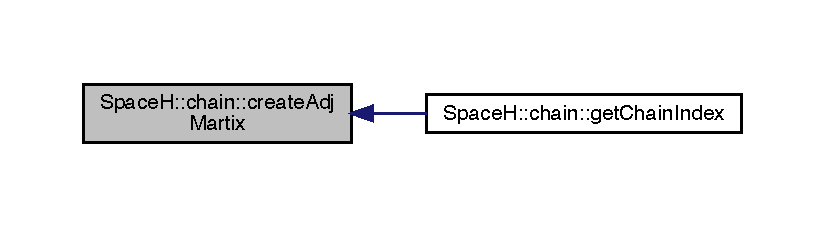
\includegraphics[width=350pt]{namespace_space_h_1_1chain_a8d2f8c8026f24294d16309c4f2e11fdb_icgraph}
\end{center}
\end{figure}
\mbox{\Hypertarget{namespace_space_h_1_1chain_a65d906373401066033d8e4a6ad581cce}\label{namespace_space_h_1_1chain_a65d906373401066033d8e4a6ad581cce}} 
\index{Space\+H\+::chain_@{Space\+H\+::chain_}!create\+Chain\+Index@{create\+Chain\+Index}}
\index{create\+Chain\+Index@{create\+Chain\+Index}!Space\+H\+::chain_@{Space\+H\+::chain_}}
\subsubsection{\texorpdfstring{create\+Chain\+Index()}{createChainIndex()}}
{\footnotesize\ttfamily template$<$typename Node\+Array , typename Index\+Array $>$ \\
void Space\+H\+::chain_\+::create\+Chain\+Index (\begin{DoxyParamCaption}\item[{Node\+Array \&}]{Adj\+Matrix,  }\item[{Index\+Array \&}]{chain_\+Index }\end{DoxyParamCaption})}



Create mapping index from adjoint matrix. 

Create mapping index from sorted elements of adjoint matrix and connect them to a chain_ consequently.
\begin{DoxyParams}{Parameters}
{\em Adj\+Matrix} & The adjoint matrix. \\
\hline
{\em chain_\+Index} & The maping index needs to be calculated as a return value. \\
\hline
\end{DoxyParams}
Here is the caller graph for this function\+:\nopagebreak
\begin{figure}[H]
\begin{center}
\leavevmode
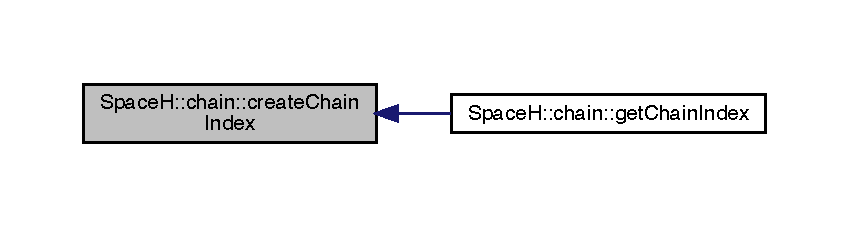
\includegraphics[width=350pt]{namespace_space_h_1_1chain_a65d906373401066033d8e4a6ad581cce_icgraph}
\end{center}
\end{figure}
\mbox{\Hypertarget{namespace_space_h_1_1chain_a9f1ed51f097bc8cf691a87b97639dde9}\label{namespace_space_h_1_1chain_a9f1ed51f097bc8cf691a87b97639dde9}} 
\index{Space\+H\+::chain_@{Space\+H\+::chain_}!get\+Chain\+Index@{get\+Chain\+Index}}
\index{get\+Chain\+Index@{get\+Chain\+Index}!Space\+H\+::chain_@{Space\+H\+::chain_}}
\subsubsection{\texorpdfstring{get\+Chain\+Index()}{getChainIndex()}}
{\footnotesize\ttfamily template$<$typename Vector\+Array , typename Index\+Array $>$ \\
void Space\+H\+::chain_\+::get\+Chain\+Index (\begin{DoxyParamCaption}\item[{const Vector\+Array \&}]{pos,  }\item[{Index\+Array \&}]{chain_\+Index }\end{DoxyParamCaption})}



Calculate the mapping index from Cartesian coordinate to chain_ coordinate.

Find the mapping index from Cartesian coordinate to chain_ coordinate. The chain_ is formed by connecting the nearest particle pairs consequently.
\begin{DoxyParams}{Parameters}
{\em pos} & The array of particle position, used to calculate the distance of particle pairs. \\
\hline
{\em chain_\+Index} & The maping index needs to be calculated as a return value. \\
\hline
\end{DoxyParams}
Here is the call graph for this function\+:\nopagebreak
\begin{figure}[H]
\begin{center}
\leavevmode
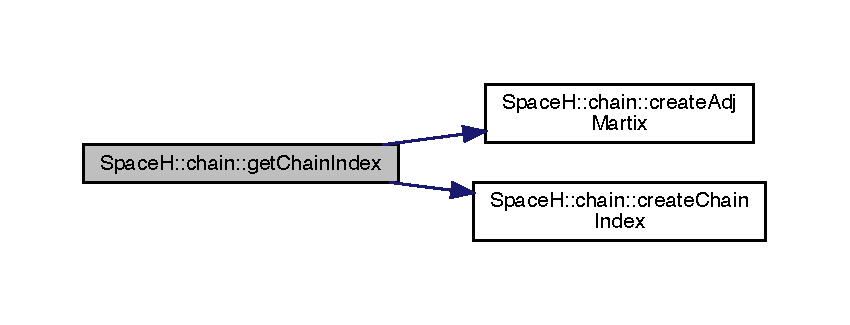
\includegraphics[width=350pt]{namespace_space_h_1_1chain_a9f1ed51f097bc8cf691a87b97639dde9_cgraph}
\end{center}
\end{figure}
Here is the caller graph for this function\+:
\nopagebreak
\begin{figure}[H]
\begin{center}
\leavevmode
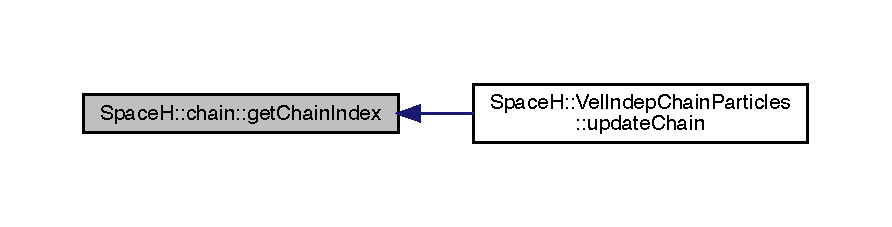
\includegraphics[width=350pt]{namespace_space_h_1_1chain_a9f1ed51f097bc8cf691a87b97639dde9_icgraph}
\end{center}
\end{figure}
\mbox{\Hypertarget{namespace_space_h_1_1chain_ab54ce920a542c01625ee7d6c625cc5c4}\label{namespace_space_h_1_1chain_ab54ce920a542c01625ee7d6c625cc5c4}} 
\index{Space\+H\+::chain_@{Space\+H\+::chain_}!is\+Diff@{is\+Diff}}
\index{is\+Diff@{is\+Diff}!Space\+H\+::chain_@{Space\+H\+::chain_}}
\subsubsection{\texorpdfstring{is\+Diff()}{isDiff()}}
{\footnotesize\ttfamily template$<$typename Index\+Array $>$ \\
bool Space\+H\+::chain_\+::is\+Diff (\begin{DoxyParamCaption}\item[{const Index\+Array \&}]{Index1,  }\item[{const Index\+Array \&}]{Index2 }\end{DoxyParamCaption})}



Check if two mapping indexes are the same. 

Checking the identity of two chain_ index mappings.
\begin{DoxyParams}{Parameters}
{\em Index1} & The first index array. \\
\hline
{\em Index2} & The second index array. \\
\hline
\end{DoxyParams}
\begin{DoxyReturn}{Returns}
boolean 
\end{DoxyReturn}
\begin{DoxyNote}{Note}
\mbox{[}2,4,5,3,1\mbox{]} is identical to \mbox{[}1,3,5,4,2\mbox{]} 
\end{DoxyNote}
Here is the caller graph for this function\+:
\nopagebreak
\begin{figure}[H]
\begin{center}
\leavevmode
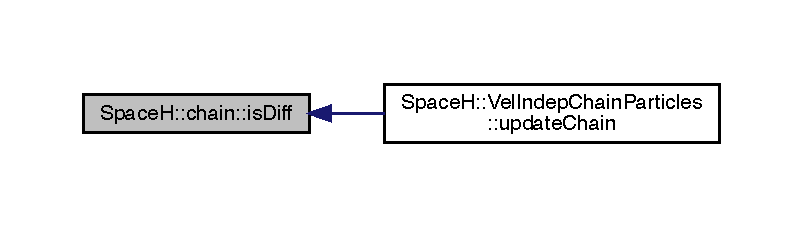
\includegraphics[width=350pt]{namespace_space_h_1_1chain_ab54ce920a542c01625ee7d6c625cc5c4_icgraph}
\end{center}
\end{figure}
\mbox{\Hypertarget{namespace_space_h_1_1chain_a1ba7809b40a52959d0566753b1c2eaee}\label{namespace_space_h_1_1chain_a1ba7809b40a52959d0566753b1c2eaee}} 
\index{Space\+H\+::chain_@{Space\+H\+::chain_}!syn\+Cartesian@{syn\+Cartesian}}
\index{syn\+Cartesian@{syn\+Cartesian}!Space\+H\+::chain_@{Space\+H\+::chain_}}
\subsubsection{\texorpdfstring{syn\+Cartesian()}{synCartesian()}}
{\footnotesize\ttfamily template$<$typename Vector\+Array , typename Index\+Array $>$ \\
void Space\+H\+::chain_\+::syn\+Cartesian (\begin{DoxyParamCaption}\item[{const Vector\+Array \&}]{chain_\+Data,  }\item[{Vector\+Array \&}]{data,  }\item[{const Index\+Array \&}]{chain_\+Index }\end{DoxyParamCaption})}



Calulate the Cartesian data from chain_ data and chain_ index mapping.


\begin{DoxyParams}{Parameters}
{\em chain_\+Data} & Data in chain_ coordinates. \\
\hline
{\em data} & Data need to be calculated in Cartesian coordinates. \\
\hline
{\em chain_\+Index} & Chain index mapping. \\
\hline
\end{DoxyParams}
\begin{DoxyNote}{Note}
This function should be a inverse transformation of \mbox{\hyperlink{namespace_space_h_1_1chain_a218de9c738267dd3efceebfda0a90a43}{syn\+Chain()}}. 
\end{DoxyNote}
Here is the caller graph for this function\+:
\nopagebreak
\begin{figure}[H]
\begin{center}
\leavevmode
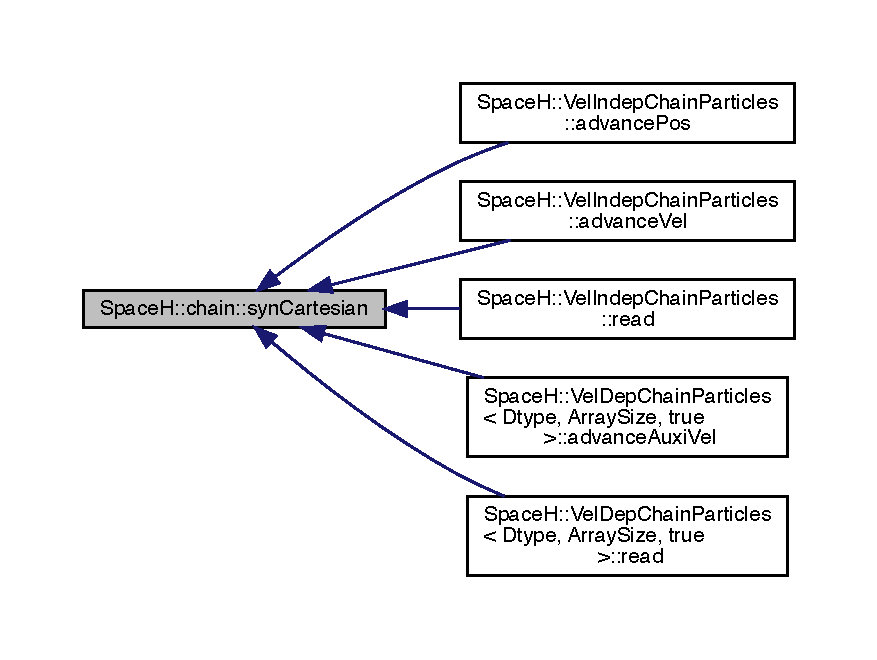
\includegraphics[width=350pt]{namespace_space_h_1_1chain_a1ba7809b40a52959d0566753b1c2eaee_icgraph}
\end{center}
\end{figure}
\mbox{\Hypertarget{namespace_space_h_1_1chain_a218de9c738267dd3efceebfda0a90a43}\label{namespace_space_h_1_1chain_a218de9c738267dd3efceebfda0a90a43}} 
\index{Space\+H\+::chain_@{Space\+H\+::chain_}!syn\+Chain@{syn\+Chain}}
\index{syn\+Chain@{syn\+Chain}!Space\+H\+::chain_@{Space\+H\+::chain_}}
\subsubsection{\texorpdfstring{syn\+Chain()}{synChain()}}
{\footnotesize\ttfamily template$<$typename Vector\+Array , typename Index\+Array $>$ \\
void Space\+H\+::chain_\+::syn\+Chain (\begin{DoxyParamCaption}\item[{const Vector\+Array \&}]{data,  }\item[{Vector\+Array \&}]{chain_\+Data,  }\item[{const Index\+Array \&}]{chain_\+Index }\end{DoxyParamCaption})}



Calulate the chain_ data from Cartesian data and chain_ index mapping.


\begin{DoxyParams}{Parameters}
{\em data} & Data in Cartesian coordinates. \\
\hline
{\em chain_\+Data} & Data need to be calculated in chain_ coordinates. \\
\hline
{\em chain_\+Index} & Chain index mapping. \\
\hline
\end{DoxyParams}
\begin{DoxyNote}{Note}
This function should be a inverse transformation of \mbox{\hyperlink{namespace_space_h_1_1chain_a1ba7809b40a52959d0566753b1c2eaee}{syn\+Cartesian()}}. 
\end{DoxyNote}
Here is the caller graph for this function\+:
\nopagebreak
\begin{figure}[H]
\begin{center}
\leavevmode
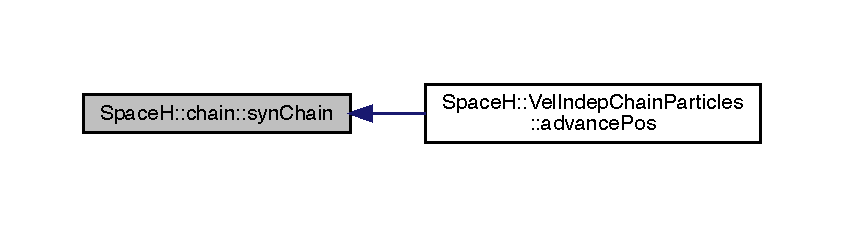
\includegraphics[width=350pt]{namespace_space_h_1_1chain_a218de9c738267dd3efceebfda0a90a43_icgraph}
\end{center}
\end{figure}
\mbox{\Hypertarget{namespace_space_h_1_1chain_a631ad6a37f246a0db64e5879825a6878}\label{namespace_space_h_1_1chain_a631ad6a37f246a0db64e5879825a6878}} 
\index{Space\+H\+::chain_@{Space\+H\+::chain_}!update\+Chain@{update\+Chain}}
\index{update\+Chain@{update\+Chain}!Space\+H\+::chain_@{Space\+H\+::chain_}}
\subsubsection{\texorpdfstring{update\+Chain()}{updateChain()}}
{\footnotesize\ttfamily template$<$typename Vector\+Array , typename Index\+Array $>$ \\
void Space\+H\+::chain_\+::update\+Chain (\begin{DoxyParamCaption}\item[{Vector\+Array \&}]{pos,  }\item[{Index\+Array \&}]{chain_\+Index,  }\item[{Index\+Array \&}]{new\+Index }\end{DoxyParamCaption})}



Update the position chain_.

Update the position chain_. Due to the evolution, the chain_ index mapping could change with time, this function is used to update the position chain_ with old chain_ data.
\begin{DoxyParams}{Parameters}
{\em pos} & The old chain_ position array needs update. \\
\hline
{\em chain_\+Index} & The old chain_ index mapping. \\
\hline
{\em new\+Index} & The new chain_ index mapping. \\
\hline
\end{DoxyParams}
Here is the caller graph for this function\+:
\nopagebreak
\begin{figure}[H]
\begin{center}
\leavevmode
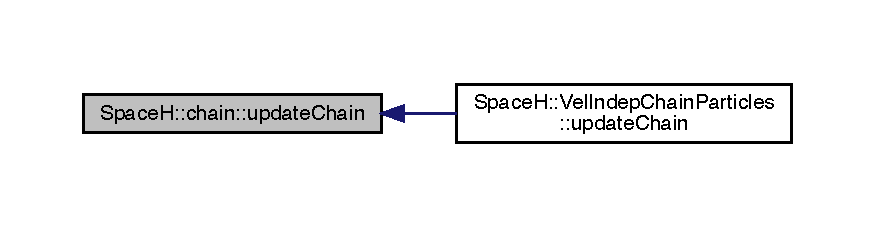
\includegraphics[width=350pt]{namespace_space_h_1_1chain_a631ad6a37f246a0db64e5879825a6878_icgraph}
\end{center}
\end{figure}

\chapter{Class Documentation}
\hypertarget{class_a_rchain}{}\section{A\+Rchain$<$ Interaction, Evolved\+Data, Regularitor $>$ Class Template Reference}
\label{class_a_rchain}\index{A\+Rchain$<$ Interaction, Evolved\+Data, Regularitor $>$@{A\+Rchain$<$ Interaction, Evolved\+Data, Regularitor $>$}}


{\ttfamily \#include $<$A\+Rchain.\+h$>$}



Inheritance diagram for A\+Rchain$<$ Interaction, Evolved\+Data, Regularitor $>$\+:\nopagebreak
\begin{figure}[H]
\begin{center}
\leavevmode
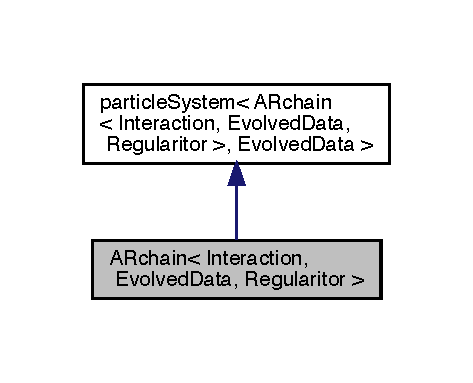
\includegraphics[width=227pt]{class_a_rchain__inherit__graph}
\end{center}
\end{figure}


Collaboration diagram for A\+Rchain$<$ Interaction, Evolved\+Data, Regularitor $>$\+:
\nopagebreak
\begin{figure}[H]
\begin{center}
\leavevmode
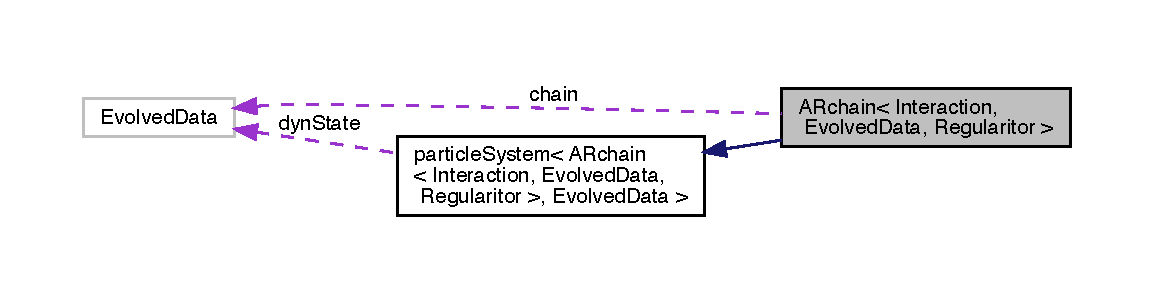
\includegraphics[width=350pt]{class_a_rchain__coll__graph}
\end{center}
\end{figure}
\subsection*{Public Types}
\begin{DoxyCompactItemize}
\item 
typedef Evolved\+Data\+::\+Scalar \mbox{\hyperlink{class_a_rchain_a707e42a79e4744424a34c9007e84ee07}{Scalar}}
\item 
typedef Evolved\+Data\+::\+Vector \mbox{\hyperlink{class_a_rchain_ab9b518a463f750eb54e002842b66e8dd}{Vector}}
\item 
typedef Evolved\+Data\+::\+Vector\+Array \mbox{\hyperlink{class_a_rchain_a019fbadb9f4e5892736d9127537338bb}{Vector\+Array}}
\item 
typedef Evolved\+Data\+::\+Scalar\+Array \mbox{\hyperlink{class_a_rchain_a206c7f2ff7ce15041a20d327d28b7be3}{Scalar\+Array}}
\item 
typedef std\+::array$<$ size\+\_\+t, Evolved\+Data\+::size()$>$ \mbox{\hyperlink{class_a_rchain_aae40d4b5881eecfc960814f9e368215d}{Index\+Array}}
\item 
typedef std\+::array$<$ \mbox{\hyperlink{class_a_rchain_a707e42a79e4744424a34c9007e84ee07}{Scalar}}, Evolved\+Data\+::volume()$>$ \mbox{\hyperlink{class_a_rchain_a829aca51411c08ffd518294770a374d5}{Plain\+Array}}
\end{DoxyCompactItemize}
\subsection*{Public Member Functions}
\begin{DoxyCompactItemize}
\item 
void \mbox{\hyperlink{class_a_rchain_a8d3ac75a6b4231e0859492257553316e}{advance\+Pos}} (\mbox{\hyperlink{class_a_rchain_a707e42a79e4744424a34c9007e84ee07}{Scalar}} time\+Step\+Size)
\item 
void \mbox{\hyperlink{class_a_rchain_a6a76ab7a095adfbf4a69226a31d866d4}{advance\+Vel}} (\mbox{\hyperlink{class_a_rchain_a707e42a79e4744424a34c9007e84ee07}{Scalar}} time\+Step\+Size)
\item 
const \mbox{\hyperlink{class_a_rchain}{A\+Rchain}} \& \mbox{\hyperlink{class_a_rchain_a7bcc783f99cad1e9113d2b505544aba1}{operator=}} (const \mbox{\hyperlink{class_a_rchain}{A\+Rchain}} \&other)
\item 
std\+::istream \& \mbox{\hyperlink{class_a_rchain_a86bd89bacf59c9c3bb0594499db82e04}{read}} (std\+::istream \&)
\item 
void \mbox{\hyperlink{class_a_rchain_a7edf1240a094d55df222c816659dced0}{load}} (\mbox{\hyperlink{class_a_rchain_a829aca51411c08ffd518294770a374d5}{Plain\+Array}} \&data)
\item 
\mbox{\hyperlink{class_a_rchain_a707e42a79e4744424a34c9007e84ee07}{Scalar}} \mbox{\hyperlink{class_a_rchain_a979a40abd086aeb411dc8e82a3bb1cdf}{time\+Scale}} (\mbox{\hyperlink{class_a_rchain_a707e42a79e4744424a34c9007e84ee07}{Scalar}} scale)
\item 
\mbox{\hyperlink{class_a_rchain_a829aca51411c08ffd518294770a374d5}{Plain\+Array}} \& \mbox{\hyperlink{class_a_rchain_aeb4d9b0a28ae3b4e4286edf838e5a905}{array}} ()
\end{DoxyCompactItemize}
\subsection*{Static Public Member Functions}
\begin{DoxyCompactItemize}
\item 
static constexpr size\+\_\+t \mbox{\hyperlink{class_a_rchain_ac612af46ce057d56dc47a6d28738a4cf}{size}} ()
\end{DoxyCompactItemize}
\subsection*{Private Member Functions}
\begin{DoxyCompactItemize}
\item 
void \mbox{\hyperlink{class_a_rchain_ac54722bde3c9a15e04dd004ebcf0db5e}{advance\+Omega}} (\mbox{\hyperlink{class_a_rchain_a707e42a79e4744424a34c9007e84ee07}{Scalar}} step\+Size)
\item 
void \mbox{\hyperlink{class_a_rchain_a1b2ae6231caeba3df20e4ab41f63a4b8}{advanceB}} (\mbox{\hyperlink{class_a_rchain_a707e42a79e4744424a34c9007e84ee07}{Scalar}} step\+Size)
\item 
void \mbox{\hyperlink{class_a_rchain_a0b073cd82321047d7fafda59cef998ef}{kick\+Vel}} (\mbox{\hyperlink{class_a_rchain_a707e42a79e4744424a34c9007e84ee07}{Scalar}} step\+Size)
\item 
void \mbox{\hyperlink{class_a_rchain_a53838a7890cee54c69786bda87dd6cd9}{kick\+Auxi\+Vel}} (\mbox{\hyperlink{class_a_rchain_a707e42a79e4744424a34c9007e84ee07}{Scalar}} step\+Size)
\item 
void \mbox{\hyperlink{class_a_rchain_a92865bff07dc16e3065a8f695120a5f5}{update\+Acc\+With}} (\mbox{\hyperlink{class_a_rchain_a019fbadb9f4e5892736d9127537338bb}{Vector\+Array}} \&\mbox{\hyperlink{classparticle_system_a545da170c4d59f18c6ddb18817cb5f3e}{vel}}, \mbox{\hyperlink{class_a_rchain_a019fbadb9f4e5892736d9127537338bb}{Vector\+Array}} \&chain\+Vel)
\item 
void \mbox{\hyperlink{class_a_rchain_a08ddf32fb537ac1556b2e4560abf3b5d}{update\+Vel\+Indep\+Acc}} ()
\item 
void \mbox{\hyperlink{class_a_rchain_ad576df000b6d9f3948eae2793c6b3c54}{update\+Chain}} ()
\end{DoxyCompactItemize}
\subsection*{Private Attributes}
\begin{DoxyCompactItemize}
\item 
Evolved\+Data \mbox{\hyperlink{class_a_rchain_af7780024bfc1beca5f5622086b909db2}{chain}}
\item 
\mbox{\hyperlink{class_a_rchain_aae40d4b5881eecfc960814f9e368215d}{Index\+Array}} \mbox{\hyperlink{class_a_rchain_a0691e6612b661e329f1fc72d4cb7c895}{chain\+Index}}
\item 
\mbox{\hyperlink{class_a_rchain_a019fbadb9f4e5892736d9127537338bb}{Vector\+Array}} \mbox{\hyperlink{class_a_rchain_a9359b4fb9f08ad849b0f1dfbdf661016}{vel\+Indep\+Acc}}
\item 
\mbox{\hyperlink{class_a_rchain_a019fbadb9f4e5892736d9127537338bb}{Vector\+Array}} \mbox{\hyperlink{class_a_rchain_a80d060a3341913f94c4bbbf2e2321b1d}{chain\+Vel\+Indep\+Acc}}
\item 
\mbox{\hyperlink{class_a_rchain_a019fbadb9f4e5892736d9127537338bb}{Vector\+Array}} \mbox{\hyperlink{class_a_rchain_a3c3a74f839bbfe5cbe1d8eb239dd8cc1}{vel\+Dep\+Acc}}
\item 
\mbox{\hyperlink{class_a_rchain_a019fbadb9f4e5892736d9127537338bb}{Vector\+Array}} \mbox{\hyperlink{class_a_rchain_a64087e0cb9cdb6b118b4a6e416d9f012}{chain\+Vel\+Dep\+Acc}}
\item 
Interaction \mbox{\hyperlink{class_a_rchain_a5ad11cefbdb69a58225b799b36dd9eee}{vel\+Dep\+Force}}
\item 
Regularitor \mbox{\hyperlink{class_a_rchain_a4dd20aa56d6a6403260ad3ced2987eb0}{regular}}
\end{DoxyCompactItemize}
\subsection*{Additional Inherited Members}


\subsection{Member Typedef Documentation}
\mbox{\Hypertarget{class_a_rchain_aae40d4b5881eecfc960814f9e368215d}\label{class_a_rchain_aae40d4b5881eecfc960814f9e368215d}} 
\index{A\+Rchain@{A\+Rchain}!Index\+Array@{Index\+Array}}
\index{Index\+Array@{Index\+Array}!A\+Rchain@{A\+Rchain}}
\subsubsection{\texorpdfstring{Index\+Array}{IndexArray}}
{\footnotesize\ttfamily template$<$typename Interaction, typename Evolved\+Data, typename Regularitor$>$ \\
typedef std\+::array$<$size\+\_\+t, Evolved\+Data\+::size()$>$ \mbox{\hyperlink{class_a_rchain}{A\+Rchain}}$<$ Interaction, Evolved\+Data, Regularitor $>$\+::\mbox{\hyperlink{class_a_rchain_aae40d4b5881eecfc960814f9e368215d}{Index\+Array}}}

\mbox{\Hypertarget{class_a_rchain_a829aca51411c08ffd518294770a374d5}\label{class_a_rchain_a829aca51411c08ffd518294770a374d5}} 
\index{A\+Rchain@{A\+Rchain}!Plain\+Array@{Plain\+Array}}
\index{Plain\+Array@{Plain\+Array}!A\+Rchain@{A\+Rchain}}
\subsubsection{\texorpdfstring{Plain\+Array}{PlainArray}}
{\footnotesize\ttfamily template$<$typename Interaction, typename Evolved\+Data, typename Regularitor$>$ \\
typedef std\+::array$<$\mbox{\hyperlink{class_a_rchain_a707e42a79e4744424a34c9007e84ee07}{Scalar}}, Evolved\+Data\+::volume()$>$ \mbox{\hyperlink{class_a_rchain}{A\+Rchain}}$<$ Interaction, Evolved\+Data, Regularitor $>$\+::\mbox{\hyperlink{class_a_rchain_a829aca51411c08ffd518294770a374d5}{Plain\+Array}}}

\mbox{\Hypertarget{class_a_rchain_a707e42a79e4744424a34c9007e84ee07}\label{class_a_rchain_a707e42a79e4744424a34c9007e84ee07}} 
\index{A\+Rchain@{A\+Rchain}!Scalar@{Scalar}}
\index{Scalar@{Scalar}!A\+Rchain@{A\+Rchain}}
\subsubsection{\texorpdfstring{Scalar}{Scalar}}
{\footnotesize\ttfamily template$<$typename Interaction, typename Evolved\+Data, typename Regularitor$>$ \\
typedef Evolved\+Data\+::\+Scalar \mbox{\hyperlink{class_a_rchain}{A\+Rchain}}$<$ Interaction, Evolved\+Data, Regularitor $>$\+::\mbox{\hyperlink{class_a_rchain_a707e42a79e4744424a34c9007e84ee07}{Scalar}}}

\mbox{\Hypertarget{class_a_rchain_a206c7f2ff7ce15041a20d327d28b7be3}\label{class_a_rchain_a206c7f2ff7ce15041a20d327d28b7be3}} 
\index{A\+Rchain@{A\+Rchain}!Scalar\+Array@{Scalar\+Array}}
\index{Scalar\+Array@{Scalar\+Array}!A\+Rchain@{A\+Rchain}}
\subsubsection{\texorpdfstring{Scalar\+Array}{ScalarArray}}
{\footnotesize\ttfamily template$<$typename Interaction, typename Evolved\+Data, typename Regularitor$>$ \\
typedef Evolved\+Data\+::\+Scalar\+Array \mbox{\hyperlink{class_a_rchain}{A\+Rchain}}$<$ Interaction, Evolved\+Data, Regularitor $>$\+::\mbox{\hyperlink{class_a_rchain_a206c7f2ff7ce15041a20d327d28b7be3}{Scalar\+Array}}}

\mbox{\Hypertarget{class_a_rchain_ab9b518a463f750eb54e002842b66e8dd}\label{class_a_rchain_ab9b518a463f750eb54e002842b66e8dd}} 
\index{A\+Rchain@{A\+Rchain}!Vector@{Vector}}
\index{Vector@{Vector}!A\+Rchain@{A\+Rchain}}
\subsubsection{\texorpdfstring{Vector}{Vector}}
{\footnotesize\ttfamily template$<$typename Interaction, typename Evolved\+Data, typename Regularitor$>$ \\
typedef Evolved\+Data\+::\+Vector \mbox{\hyperlink{class_a_rchain}{A\+Rchain}}$<$ Interaction, Evolved\+Data, Regularitor $>$\+::\mbox{\hyperlink{class_a_rchain_ab9b518a463f750eb54e002842b66e8dd}{Vector}}}

\mbox{\Hypertarget{class_a_rchain_a019fbadb9f4e5892736d9127537338bb}\label{class_a_rchain_a019fbadb9f4e5892736d9127537338bb}} 
\index{A\+Rchain@{A\+Rchain}!Vector\+Array@{Vector\+Array}}
\index{Vector\+Array@{Vector\+Array}!A\+Rchain@{A\+Rchain}}
\subsubsection{\texorpdfstring{Vector\+Array}{VectorArray}}
{\footnotesize\ttfamily template$<$typename Interaction, typename Evolved\+Data, typename Regularitor$>$ \\
typedef Evolved\+Data\+::\+Vector\+Array \mbox{\hyperlink{class_a_rchain}{A\+Rchain}}$<$ Interaction, Evolved\+Data, Regularitor $>$\+::\mbox{\hyperlink{class_a_rchain_a019fbadb9f4e5892736d9127537338bb}{Vector\+Array}}}



\subsection{Member Function Documentation}
\mbox{\Hypertarget{class_a_rchain_a1b2ae6231caeba3df20e4ab41f63a4b8}\label{class_a_rchain_a1b2ae6231caeba3df20e4ab41f63a4b8}} 
\index{A\+Rchain@{A\+Rchain}!advanceB@{advanceB}}
\index{advanceB@{advanceB}!A\+Rchain@{A\+Rchain}}
\subsubsection{\texorpdfstring{advance\+B()}{advanceB()}}
{\footnotesize\ttfamily template$<$typename Interaction , typename Evolved\+Data , typename Regularitor $>$ \\
void \mbox{\hyperlink{class_a_rchain}{A\+Rchain}}$<$ Interaction, Evolved\+Data, Regularitor $>$\+::advanceB (\begin{DoxyParamCaption}\item[{\mbox{\hyperlink{class_a_rchain_a707e42a79e4744424a34c9007e84ee07}{Scalar}}}]{step\+Size }\end{DoxyParamCaption})\hspace{0.3cm}{\ttfamily [private]}}

Here is the call graph for this function\+:
\nopagebreak
\begin{figure}[H]
\begin{center}
\leavevmode
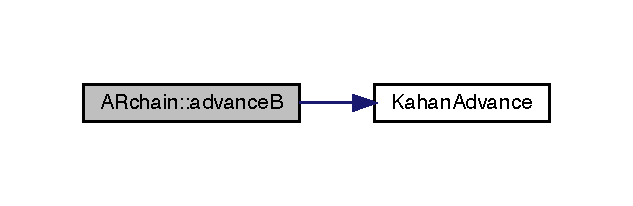
\includegraphics[width=304pt]{class_a_rchain_a1b2ae6231caeba3df20e4ab41f63a4b8_cgraph}
\end{center}
\end{figure}
\mbox{\Hypertarget{class_a_rchain_ac54722bde3c9a15e04dd004ebcf0db5e}\label{class_a_rchain_ac54722bde3c9a15e04dd004ebcf0db5e}} 
\index{A\+Rchain@{A\+Rchain}!advance\+Omega@{advance\+Omega}}
\index{advance\+Omega@{advance\+Omega}!A\+Rchain@{A\+Rchain}}
\subsubsection{\texorpdfstring{advance\+Omega()}{advanceOmega()}}
{\footnotesize\ttfamily template$<$typename Interaction , typename Evolved\+Data , typename Regularitor $>$ \\
void \mbox{\hyperlink{class_a_rchain}{A\+Rchain}}$<$ Interaction, Evolved\+Data, Regularitor $>$\+::advance\+Omega (\begin{DoxyParamCaption}\item[{\mbox{\hyperlink{class_a_rchain_a707e42a79e4744424a34c9007e84ee07}{Scalar}}}]{step\+Size }\end{DoxyParamCaption})\hspace{0.3cm}{\ttfamily [private]}}

Here is the call graph for this function\+:
\nopagebreak
\begin{figure}[H]
\begin{center}
\leavevmode
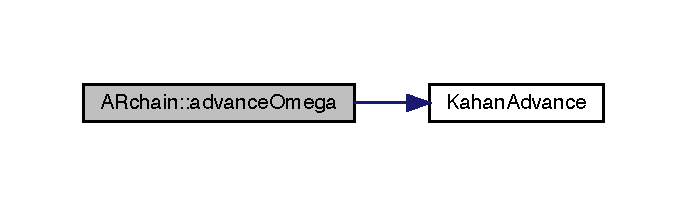
\includegraphics[width=330pt]{class_a_rchain_ac54722bde3c9a15e04dd004ebcf0db5e_cgraph}
\end{center}
\end{figure}
\mbox{\Hypertarget{class_a_rchain_a8d3ac75a6b4231e0859492257553316e}\label{class_a_rchain_a8d3ac75a6b4231e0859492257553316e}} 
\index{A\+Rchain@{A\+Rchain}!advance\+Pos@{advance\+Pos}}
\index{advance\+Pos@{advance\+Pos}!A\+Rchain@{A\+Rchain}}
\subsubsection{\texorpdfstring{advance\+Pos()}{advancePos()}}
{\footnotesize\ttfamily template$<$typename Interaction , typename Evolved\+Data , typename Regularitor $>$ \\
void \mbox{\hyperlink{class_a_rchain}{A\+Rchain}}$<$ Interaction, Evolved\+Data, Regularitor $>$\+::advance\+Pos (\begin{DoxyParamCaption}\item[{\mbox{\hyperlink{class_a_rchain_a707e42a79e4744424a34c9007e84ee07}{Scalar}}}]{time\+Step\+Size }\end{DoxyParamCaption})}

Here is the call graph for this function\+:
\nopagebreak
\begin{figure}[H]
\begin{center}
\leavevmode
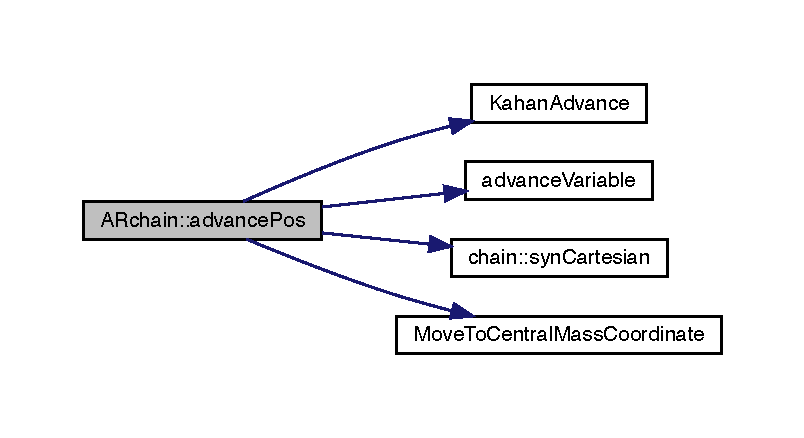
\includegraphics[width=350pt]{class_a_rchain_a8d3ac75a6b4231e0859492257553316e_cgraph}
\end{center}
\end{figure}
\mbox{\Hypertarget{class_a_rchain_a6a76ab7a095adfbf4a69226a31d866d4}\label{class_a_rchain_a6a76ab7a095adfbf4a69226a31d866d4}} 
\index{A\+Rchain@{A\+Rchain}!advance\+Vel@{advance\+Vel}}
\index{advance\+Vel@{advance\+Vel}!A\+Rchain@{A\+Rchain}}
\subsubsection{\texorpdfstring{advance\+Vel()}{advanceVel()}}
{\footnotesize\ttfamily template$<$typename Interaction , typename Evolved\+Data , typename Regularitor $>$ \\
void \mbox{\hyperlink{class_a_rchain}{A\+Rchain}}$<$ Interaction, Evolved\+Data, Regularitor $>$\+::advance\+Vel (\begin{DoxyParamCaption}\item[{\mbox{\hyperlink{class_a_rchain_a707e42a79e4744424a34c9007e84ee07}{Scalar}}}]{time\+Step\+Size }\end{DoxyParamCaption})}

\mbox{\Hypertarget{class_a_rchain_aeb4d9b0a28ae3b4e4286edf838e5a905}\label{class_a_rchain_aeb4d9b0a28ae3b4e4286edf838e5a905}} 
\index{A\+Rchain@{A\+Rchain}!array@{array}}
\index{array@{array}!A\+Rchain@{A\+Rchain}}
\subsubsection{\texorpdfstring{array()}{array()}}
{\footnotesize\ttfamily template$<$typename Interaction, typename Evolved\+Data, typename Regularitor$>$ \\
\mbox{\hyperlink{class_a_rchain_a829aca51411c08ffd518294770a374d5}{Plain\+Array}}\& \mbox{\hyperlink{class_a_rchain}{A\+Rchain}}$<$ Interaction, Evolved\+Data, Regularitor $>$\+::array (\begin{DoxyParamCaption}{ }\end{DoxyParamCaption})\hspace{0.3cm}{\ttfamily [inline]}}

\mbox{\Hypertarget{class_a_rchain_a53838a7890cee54c69786bda87dd6cd9}\label{class_a_rchain_a53838a7890cee54c69786bda87dd6cd9}} 
\index{A\+Rchain@{A\+Rchain}!kick\+Auxi\+Vel@{kick\+Auxi\+Vel}}
\index{kick\+Auxi\+Vel@{kick\+Auxi\+Vel}!A\+Rchain@{A\+Rchain}}
\subsubsection{\texorpdfstring{kick\+Auxi\+Vel()}{kickAuxiVel()}}
{\footnotesize\ttfamily template$<$typename Interaction , typename Evolved\+Data , typename Regularitor $>$ \\
void \mbox{\hyperlink{class_a_rchain}{A\+Rchain}}$<$ Interaction, Evolved\+Data, Regularitor $>$\+::kick\+Auxi\+Vel (\begin{DoxyParamCaption}\item[{\mbox{\hyperlink{class_a_rchain_a707e42a79e4744424a34c9007e84ee07}{Scalar}}}]{step\+Size }\end{DoxyParamCaption})\hspace{0.3cm}{\ttfamily [private]}}

Here is the call graph for this function\+:
\nopagebreak
\begin{figure}[H]
\begin{center}
\leavevmode
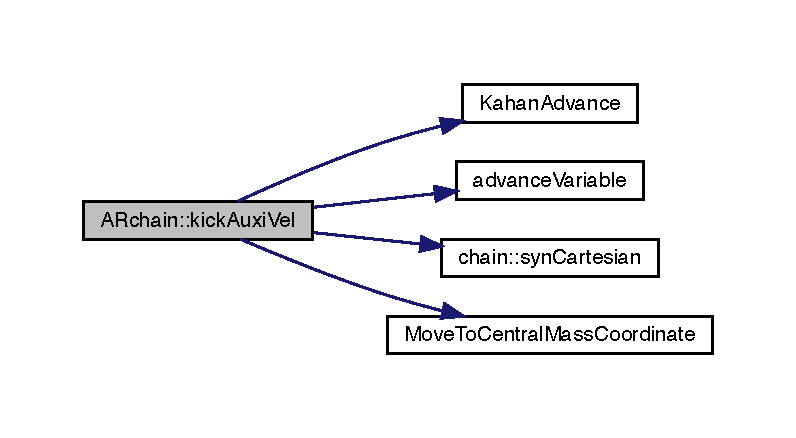
\includegraphics[width=350pt]{class_a_rchain_a53838a7890cee54c69786bda87dd6cd9_cgraph}
\end{center}
\end{figure}
\mbox{\Hypertarget{class_a_rchain_a0b073cd82321047d7fafda59cef998ef}\label{class_a_rchain_a0b073cd82321047d7fafda59cef998ef}} 
\index{A\+Rchain@{A\+Rchain}!kick\+Vel@{kick\+Vel}}
\index{kick\+Vel@{kick\+Vel}!A\+Rchain@{A\+Rchain}}
\subsubsection{\texorpdfstring{kick\+Vel()}{kickVel()}}
{\footnotesize\ttfamily template$<$typename Interaction , typename Evolved\+Data , typename Regularitor $>$ \\
void \mbox{\hyperlink{class_a_rchain}{A\+Rchain}}$<$ Interaction, Evolved\+Data, Regularitor $>$\+::kick\+Vel (\begin{DoxyParamCaption}\item[{\mbox{\hyperlink{class_a_rchain_a707e42a79e4744424a34c9007e84ee07}{Scalar}}}]{step\+Size }\end{DoxyParamCaption})\hspace{0.3cm}{\ttfamily [private]}}

Here is the call graph for this function\+:
\nopagebreak
\begin{figure}[H]
\begin{center}
\leavevmode
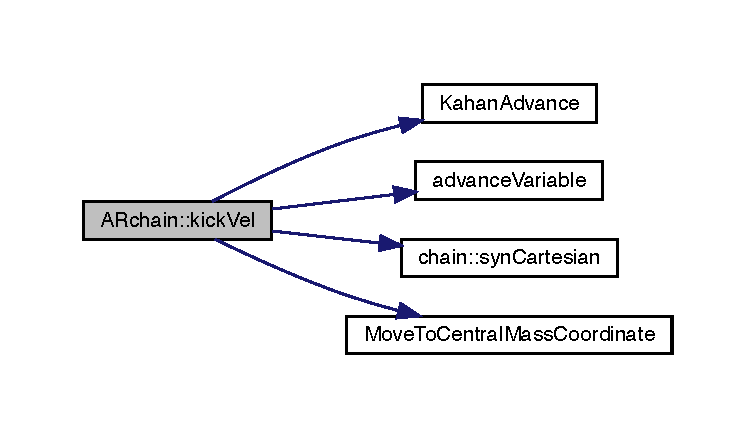
\includegraphics[width=350pt]{class_a_rchain_a0b073cd82321047d7fafda59cef998ef_cgraph}
\end{center}
\end{figure}
\mbox{\Hypertarget{class_a_rchain_a7edf1240a094d55df222c816659dced0}\label{class_a_rchain_a7edf1240a094d55df222c816659dced0}} 
\index{A\+Rchain@{A\+Rchain}!load@{load}}
\index{load@{load}!A\+Rchain@{A\+Rchain}}
\subsubsection{\texorpdfstring{load()}{load()}}
{\footnotesize\ttfamily template$<$typename Interaction , typename Evolved\+Data , typename Regularitor $>$ \\
void \mbox{\hyperlink{class_a_rchain}{A\+Rchain}}$<$ Interaction, Evolved\+Data, Regularitor $>$\+::load (\begin{DoxyParamCaption}\item[{\mbox{\hyperlink{class_a_rchain_a829aca51411c08ffd518294770a374d5}{Plain\+Array}} \&}]{data }\end{DoxyParamCaption})}

Here is the call graph for this function\+:
\nopagebreak
\begin{figure}[H]
\begin{center}
\leavevmode
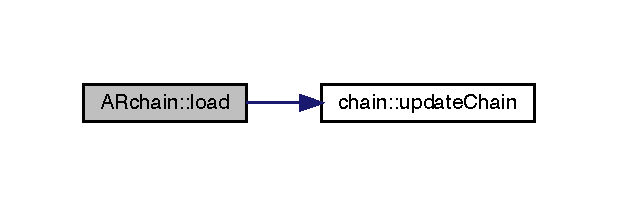
\includegraphics[width=296pt]{class_a_rchain_a7edf1240a094d55df222c816659dced0_cgraph}
\end{center}
\end{figure}
\mbox{\Hypertarget{class_a_rchain_a7bcc783f99cad1e9113d2b505544aba1}\label{class_a_rchain_a7bcc783f99cad1e9113d2b505544aba1}} 
\index{A\+Rchain@{A\+Rchain}!operator=@{operator=}}
\index{operator=@{operator=}!A\+Rchain@{A\+Rchain}}
\subsubsection{\texorpdfstring{operator=()}{operator=()}}
{\footnotesize\ttfamily template$<$typename Interaction , typename Evolved\+Data , typename Regularitor $>$ \\
const \mbox{\hyperlink{class_a_rchain}{A\+Rchain}}$<$ Interaction, Evolved\+Data, Regularitor $>$ \& \mbox{\hyperlink{class_a_rchain}{A\+Rchain}}$<$ Interaction, Evolved\+Data, Regularitor $>$\+::operator= (\begin{DoxyParamCaption}\item[{const \mbox{\hyperlink{class_a_rchain}{A\+Rchain}}$<$ Interaction, Evolved\+Data, Regularitor $>$ \&}]{other }\end{DoxyParamCaption})}

\mbox{\Hypertarget{class_a_rchain_a86bd89bacf59c9c3bb0594499db82e04}\label{class_a_rchain_a86bd89bacf59c9c3bb0594499db82e04}} 
\index{A\+Rchain@{A\+Rchain}!read@{read}}
\index{read@{read}!A\+Rchain@{A\+Rchain}}
\subsubsection{\texorpdfstring{read()}{read()}}
{\footnotesize\ttfamily template$<$typename Interaction , typename Evolved\+Data , typename Regularitor $>$ \\
std\+::istream \& \mbox{\hyperlink{class_a_rchain}{A\+Rchain}}$<$ Interaction, Evolved\+Data, Regularitor $>$\+::read (\begin{DoxyParamCaption}\item[{std\+::istream \&}]{input }\end{DoxyParamCaption})}

Here is the call graph for this function\+:
\nopagebreak
\begin{figure}[H]
\begin{center}
\leavevmode
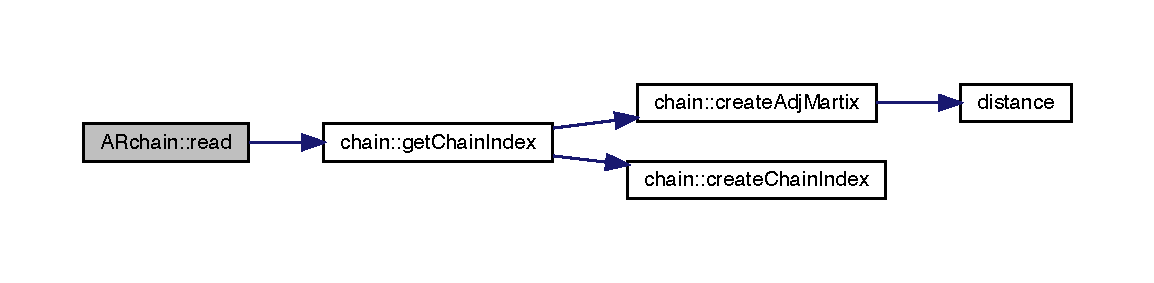
\includegraphics[width=350pt]{class_a_rchain_a86bd89bacf59c9c3bb0594499db82e04_cgraph}
\end{center}
\end{figure}
\mbox{\Hypertarget{class_a_rchain_ac612af46ce057d56dc47a6d28738a4cf}\label{class_a_rchain_ac612af46ce057d56dc47a6d28738a4cf}} 
\index{A\+Rchain@{A\+Rchain}!size@{size}}
\index{size@{size}!A\+Rchain@{A\+Rchain}}
\subsubsection{\texorpdfstring{size()}{size()}}
{\footnotesize\ttfamily template$<$typename Interaction, typename Evolved\+Data, typename Regularitor$>$ \\
static constexpr size\+\_\+t \mbox{\hyperlink{class_a_rchain}{A\+Rchain}}$<$ Interaction, Evolved\+Data, Regularitor $>$\+::size (\begin{DoxyParamCaption}{ }\end{DoxyParamCaption})\hspace{0.3cm}{\ttfamily [inline]}, {\ttfamily [static]}}

\mbox{\Hypertarget{class_a_rchain_a979a40abd086aeb411dc8e82a3bb1cdf}\label{class_a_rchain_a979a40abd086aeb411dc8e82a3bb1cdf}} 
\index{A\+Rchain@{A\+Rchain}!time\+Scale@{time\+Scale}}
\index{time\+Scale@{time\+Scale}!A\+Rchain@{A\+Rchain}}
\subsubsection{\texorpdfstring{time\+Scale()}{timeScale()}}
{\footnotesize\ttfamily template$<$typename Interaction , typename Evolved\+Data , typename Regularitor $>$ \\
Evolved\+Data\+::\+Scalar \mbox{\hyperlink{class_a_rchain}{A\+Rchain}}$<$ Interaction, Evolved\+Data, Regularitor $>$\+::time\+Scale (\begin{DoxyParamCaption}\item[{\mbox{\hyperlink{class_a_rchain_a707e42a79e4744424a34c9007e84ee07}{Scalar}}}]{scale }\end{DoxyParamCaption})}

\mbox{\Hypertarget{class_a_rchain_a92865bff07dc16e3065a8f695120a5f5}\label{class_a_rchain_a92865bff07dc16e3065a8f695120a5f5}} 
\index{A\+Rchain@{A\+Rchain}!update\+Acc\+With@{update\+Acc\+With}}
\index{update\+Acc\+With@{update\+Acc\+With}!A\+Rchain@{A\+Rchain}}
\subsubsection{\texorpdfstring{update\+Acc\+With()}{updateAccWith()}}
{\footnotesize\ttfamily template$<$typename Interaction , typename Evolved\+Data , typename Regularitor $>$ \\
void \mbox{\hyperlink{class_a_rchain}{A\+Rchain}}$<$ Interaction, Evolved\+Data, Regularitor $>$\+::update\+Acc\+With (\begin{DoxyParamCaption}\item[{\mbox{\hyperlink{class_a_rchain_a019fbadb9f4e5892736d9127537338bb}{Vector\+Array}} \&}]{vel,  }\item[{\mbox{\hyperlink{class_a_rchain_a019fbadb9f4e5892736d9127537338bb}{Vector\+Array}} \&}]{chain\+Vel }\end{DoxyParamCaption})\hspace{0.3cm}{\ttfamily [private]}}

\mbox{\Hypertarget{class_a_rchain_ad576df000b6d9f3948eae2793c6b3c54}\label{class_a_rchain_ad576df000b6d9f3948eae2793c6b3c54}} 
\index{A\+Rchain@{A\+Rchain}!update\+Chain@{update\+Chain}}
\index{update\+Chain@{update\+Chain}!A\+Rchain@{A\+Rchain}}
\subsubsection{\texorpdfstring{update\+Chain()}{updateChain()}}
{\footnotesize\ttfamily template$<$typename Interaction , typename Evolved\+Data , typename Regularitor $>$ \\
void \mbox{\hyperlink{class_a_rchain}{A\+Rchain}}$<$ Interaction, Evolved\+Data, Regularitor $>$\+::update\+Chain (\begin{DoxyParamCaption}{ }\end{DoxyParamCaption})\hspace{0.3cm}{\ttfamily [private]}}

Here is the call graph for this function\+:
\nopagebreak
\begin{figure}[H]
\begin{center}
\leavevmode
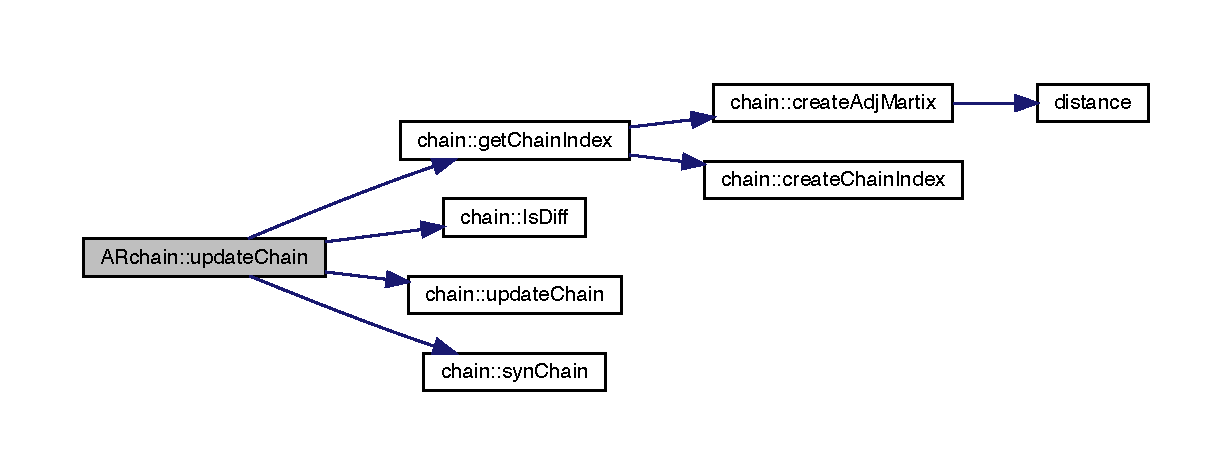
\includegraphics[width=350pt]{class_a_rchain_ad576df000b6d9f3948eae2793c6b3c54_cgraph}
\end{center}
\end{figure}
\mbox{\Hypertarget{class_a_rchain_a08ddf32fb537ac1556b2e4560abf3b5d}\label{class_a_rchain_a08ddf32fb537ac1556b2e4560abf3b5d}} 
\index{A\+Rchain@{A\+Rchain}!update\+Vel\+Indep\+Acc@{update\+Vel\+Indep\+Acc}}
\index{update\+Vel\+Indep\+Acc@{update\+Vel\+Indep\+Acc}!A\+Rchain@{A\+Rchain}}
\subsubsection{\texorpdfstring{update\+Vel\+Indep\+Acc()}{updateVelIndepAcc()}}
{\footnotesize\ttfamily template$<$typename Interaction , typename Evolved\+Data , typename Regularitor $>$ \\
void \mbox{\hyperlink{class_a_rchain}{A\+Rchain}}$<$ Interaction, Evolved\+Data, Regularitor $>$\+::update\+Vel\+Indep\+Acc (\begin{DoxyParamCaption}{ }\end{DoxyParamCaption})\hspace{0.3cm}{\ttfamily [private]}}



\subsection{Member Data Documentation}
\mbox{\Hypertarget{class_a_rchain_af7780024bfc1beca5f5622086b909db2}\label{class_a_rchain_af7780024bfc1beca5f5622086b909db2}} 
\index{A\+Rchain@{A\+Rchain}!chain@{chain}}
\index{chain@{chain}!A\+Rchain@{A\+Rchain}}
\subsubsection{\texorpdfstring{chain}{chain}}
{\footnotesize\ttfamily template$<$typename Interaction, typename Evolved\+Data, typename Regularitor$>$ \\
Evolved\+Data \mbox{\hyperlink{class_a_rchain}{A\+Rchain}}$<$ Interaction, Evolved\+Data, Regularitor $>$\+::chain\hspace{0.3cm}{\ttfamily [private]}}

\mbox{\Hypertarget{class_a_rchain_a0691e6612b661e329f1fc72d4cb7c895}\label{class_a_rchain_a0691e6612b661e329f1fc72d4cb7c895}} 
\index{A\+Rchain@{A\+Rchain}!chain\+Index@{chain\+Index}}
\index{chain\+Index@{chain\+Index}!A\+Rchain@{A\+Rchain}}
\subsubsection{\texorpdfstring{chain\+Index}{chainIndex}}
{\footnotesize\ttfamily template$<$typename Interaction, typename Evolved\+Data, typename Regularitor$>$ \\
\mbox{\hyperlink{class_a_rchain_aae40d4b5881eecfc960814f9e368215d}{Index\+Array}} \mbox{\hyperlink{class_a_rchain}{A\+Rchain}}$<$ Interaction, Evolved\+Data, Regularitor $>$\+::chain\+Index\hspace{0.3cm}{\ttfamily [private]}}

\mbox{\Hypertarget{class_a_rchain_a64087e0cb9cdb6b118b4a6e416d9f012}\label{class_a_rchain_a64087e0cb9cdb6b118b4a6e416d9f012}} 
\index{A\+Rchain@{A\+Rchain}!chain\+Vel\+Dep\+Acc@{chain\+Vel\+Dep\+Acc}}
\index{chain\+Vel\+Dep\+Acc@{chain\+Vel\+Dep\+Acc}!A\+Rchain@{A\+Rchain}}
\subsubsection{\texorpdfstring{chain\+Vel\+Dep\+Acc}{chainVelDepAcc}}
{\footnotesize\ttfamily template$<$typename Interaction, typename Evolved\+Data, typename Regularitor$>$ \\
\mbox{\hyperlink{class_a_rchain_a019fbadb9f4e5892736d9127537338bb}{Vector\+Array}} \mbox{\hyperlink{class_a_rchain}{A\+Rchain}}$<$ Interaction, Evolved\+Data, Regularitor $>$\+::chain\+Vel\+Dep\+Acc\hspace{0.3cm}{\ttfamily [private]}}

\mbox{\Hypertarget{class_a_rchain_a80d060a3341913f94c4bbbf2e2321b1d}\label{class_a_rchain_a80d060a3341913f94c4bbbf2e2321b1d}} 
\index{A\+Rchain@{A\+Rchain}!chain\+Vel\+Indep\+Acc@{chain\+Vel\+Indep\+Acc}}
\index{chain\+Vel\+Indep\+Acc@{chain\+Vel\+Indep\+Acc}!A\+Rchain@{A\+Rchain}}
\subsubsection{\texorpdfstring{chain\+Vel\+Indep\+Acc}{chainVelIndepAcc}}
{\footnotesize\ttfamily template$<$typename Interaction, typename Evolved\+Data, typename Regularitor$>$ \\
\mbox{\hyperlink{class_a_rchain_a019fbadb9f4e5892736d9127537338bb}{Vector\+Array}} \mbox{\hyperlink{class_a_rchain}{A\+Rchain}}$<$ Interaction, Evolved\+Data, Regularitor $>$\+::chain\+Vel\+Indep\+Acc\hspace{0.3cm}{\ttfamily [private]}}

\mbox{\Hypertarget{class_a_rchain_a4dd20aa56d6a6403260ad3ced2987eb0}\label{class_a_rchain_a4dd20aa56d6a6403260ad3ced2987eb0}} 
\index{A\+Rchain@{A\+Rchain}!regular@{regular}}
\index{regular@{regular}!A\+Rchain@{A\+Rchain}}
\subsubsection{\texorpdfstring{regular}{regular}}
{\footnotesize\ttfamily template$<$typename Interaction, typename Evolved\+Data, typename Regularitor$>$ \\
Regularitor \mbox{\hyperlink{class_a_rchain}{A\+Rchain}}$<$ Interaction, Evolved\+Data, Regularitor $>$\+::regular\hspace{0.3cm}{\ttfamily [private]}}

\mbox{\Hypertarget{class_a_rchain_a3c3a74f839bbfe5cbe1d8eb239dd8cc1}\label{class_a_rchain_a3c3a74f839bbfe5cbe1d8eb239dd8cc1}} 
\index{A\+Rchain@{A\+Rchain}!vel\+Dep\+Acc@{vel\+Dep\+Acc}}
\index{vel\+Dep\+Acc@{vel\+Dep\+Acc}!A\+Rchain@{A\+Rchain}}
\subsubsection{\texorpdfstring{vel\+Dep\+Acc}{velDepAcc}}
{\footnotesize\ttfamily template$<$typename Interaction, typename Evolved\+Data, typename Regularitor$>$ \\
\mbox{\hyperlink{class_a_rchain_a019fbadb9f4e5892736d9127537338bb}{Vector\+Array}} \mbox{\hyperlink{class_a_rchain}{A\+Rchain}}$<$ Interaction, Evolved\+Data, Regularitor $>$\+::vel\+Dep\+Acc\hspace{0.3cm}{\ttfamily [private]}}

\mbox{\Hypertarget{class_a_rchain_a5ad11cefbdb69a58225b799b36dd9eee}\label{class_a_rchain_a5ad11cefbdb69a58225b799b36dd9eee}} 
\index{A\+Rchain@{A\+Rchain}!vel\+Dep\+Force@{vel\+Dep\+Force}}
\index{vel\+Dep\+Force@{vel\+Dep\+Force}!A\+Rchain@{A\+Rchain}}
\subsubsection{\texorpdfstring{vel\+Dep\+Force}{velDepForce}}
{\footnotesize\ttfamily template$<$typename Interaction, typename Evolved\+Data, typename Regularitor$>$ \\
Interaction \mbox{\hyperlink{class_a_rchain}{A\+Rchain}}$<$ Interaction, Evolved\+Data, Regularitor $>$\+::vel\+Dep\+Force\hspace{0.3cm}{\ttfamily [private]}}

\mbox{\Hypertarget{class_a_rchain_a9359b4fb9f08ad849b0f1dfbdf661016}\label{class_a_rchain_a9359b4fb9f08ad849b0f1dfbdf661016}} 
\index{A\+Rchain@{A\+Rchain}!vel\+Indep\+Acc@{vel\+Indep\+Acc}}
\index{vel\+Indep\+Acc@{vel\+Indep\+Acc}!A\+Rchain@{A\+Rchain}}
\subsubsection{\texorpdfstring{vel\+Indep\+Acc}{velIndepAcc}}
{\footnotesize\ttfamily template$<$typename Interaction, typename Evolved\+Data, typename Regularitor$>$ \\
\mbox{\hyperlink{class_a_rchain_a019fbadb9f4e5892736d9127537338bb}{Vector\+Array}} \mbox{\hyperlink{class_a_rchain}{A\+Rchain}}$<$ Interaction, Evolved\+Data, Regularitor $>$\+::vel\+Indep\+Acc\hspace{0.3cm}{\ttfamily [private]}}



The documentation for this class was generated from the following file\+:\begin{DoxyCompactItemize}
\item 
particle\+System/\mbox{\hyperlink{_a_rchain_8h}{A\+Rchain.\+h}}\end{DoxyCompactItemize}

\hypertarget{struct_space_h_1_1_array_wrapper}{}\section{SpaceH\+:\+:Array\+Wrapper$<$ T, S $>$ Struct Template Reference}
\label{struct_space_h_1_1_array_wrapper}\index{Space\+H\+::\+Array\+Wrapper$<$ T, S $>$@{Space\+H\+::\+Array\+Wrapper$<$ T, S $>$}}


{\ttfamily \#include $<$proto\+Type.\+h$>$}



Inheritance diagram for SpaceH\+:\+:Array\+Wrapper$<$ T, S $>$\+:\nopagebreak
\begin{figure}[H]
\begin{center}
\leavevmode
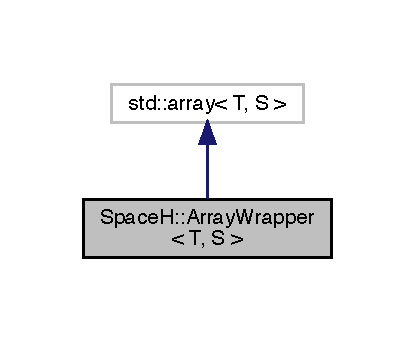
\includegraphics[width=199pt]{struct_space_h_1_1_array_wrapper__inherit__graph}
\end{center}
\end{figure}


Collaboration diagram for SpaceH\+:\+:Array\+Wrapper$<$ T, S $>$\+:\nopagebreak
\begin{figure}[H]
\begin{center}
\leavevmode
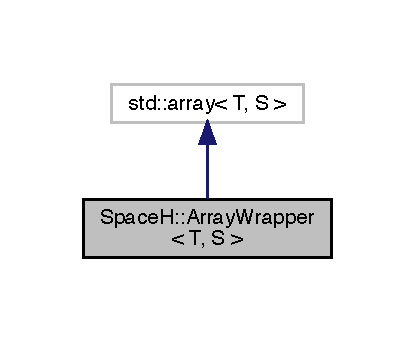
\includegraphics[width=199pt]{struct_space_h_1_1_array_wrapper__coll__graph}
\end{center}
\end{figure}
\subsection*{Public Member Functions}
\begin{DoxyCompactItemize}
\item 
void \mbox{\hyperlink{struct_space_h_1_1_array_wrapper_ac388a0420df96cf7fa128af10bd91514}{clear}} ()
\item 
void \mbox{\hyperlink{struct_space_h_1_1_array_wrapper_a0b6c9b3a863b31b77f67a61afdd3f6f1}{reserve}} (size\+\_\+t new\+\_\+cap)
\item 
void \mbox{\hyperlink{struct_space_h_1_1_array_wrapper_a5198ec13cd7200e87bd786bcc1692884}{resize}} (size\+\_\+t new\+\_\+size)
\end{DoxyCompactItemize}


\subsection{Member Function Documentation}
\mbox{\Hypertarget{struct_space_h_1_1_array_wrapper_ac388a0420df96cf7fa128af10bd91514}\label{struct_space_h_1_1_array_wrapper_ac388a0420df96cf7fa128af10bd91514}} 
\index{Space\+H\+::\+Array\+Wrapper@{Space\+H\+::\+Array\+Wrapper}!clear@{clear}}
\index{clear@{clear}!Space\+H\+::\+Array\+Wrapper@{Space\+H\+::\+Array\+Wrapper}}
\subsubsection{\texorpdfstring{clear()}{clear()}}
{\footnotesize\ttfamily template$<$typename T , size\+\_\+t S$>$ \\
void \mbox{\hyperlink{struct_space_h_1_1_array_wrapper}{Space\+H\+::\+Array\+Wrapper}}$<$ T, S $>$\+::clear (\begin{DoxyParamCaption}{ }\end{DoxyParamCaption})\hspace{0.3cm}{\ttfamily [inline]}}

\mbox{\Hypertarget{struct_space_h_1_1_array_wrapper_a0b6c9b3a863b31b77f67a61afdd3f6f1}\label{struct_space_h_1_1_array_wrapper_a0b6c9b3a863b31b77f67a61afdd3f6f1}} 
\index{Space\+H\+::\+Array\+Wrapper@{Space\+H\+::\+Array\+Wrapper}!reserve@{reserve}}
\index{reserve@{reserve}!Space\+H\+::\+Array\+Wrapper@{Space\+H\+::\+Array\+Wrapper}}
\subsubsection{\texorpdfstring{reserve()}{reserve()}}
{\footnotesize\ttfamily template$<$typename T , size\+\_\+t S$>$ \\
void \mbox{\hyperlink{struct_space_h_1_1_array_wrapper}{Space\+H\+::\+Array\+Wrapper}}$<$ T, S $>$\+::reserve (\begin{DoxyParamCaption}\item[{size\+\_\+t}]{new\+\_\+cap }\end{DoxyParamCaption})\hspace{0.3cm}{\ttfamily [inline]}}

\mbox{\Hypertarget{struct_space_h_1_1_array_wrapper_a5198ec13cd7200e87bd786bcc1692884}\label{struct_space_h_1_1_array_wrapper_a5198ec13cd7200e87bd786bcc1692884}} 
\index{Space\+H\+::\+Array\+Wrapper@{Space\+H\+::\+Array\+Wrapper}!resize@{resize}}
\index{resize@{resize}!Space\+H\+::\+Array\+Wrapper@{Space\+H\+::\+Array\+Wrapper}}
\subsubsection{\texorpdfstring{resize()}{resize()}}
{\footnotesize\ttfamily template$<$typename T , size\+\_\+t S$>$ \\
void \mbox{\hyperlink{struct_space_h_1_1_array_wrapper}{Space\+H\+::\+Array\+Wrapper}}$<$ T, S $>$\+::resize (\begin{DoxyParamCaption}\item[{size\+\_\+t}]{new\+\_\+size }\end{DoxyParamCaption})\hspace{0.3cm}{\ttfamily [inline]}}



The documentation for this struct was generated from the following file\+:\begin{DoxyCompactItemize}
\item 
\mbox{\hyperlink{proto_type_8h}{proto\+Type.\+h}}\end{DoxyCompactItemize}

\hypertarget{struct_space_h_1_1_array_wrapper_3_01_t_00_01_d_y_n_a_m_i_c_a_l_01_4}{}\section{SpaceH\+:\+:Array\+Wrapper$<$ T, D\+Y\+N\+A\+M\+I\+C\+AL $>$ Struct Template Reference}
\label{struct_space_h_1_1_array_wrapper_3_01_t_00_01_d_y_n_a_m_i_c_a_l_01_4}\index{Space\+H\+::\+Array\+Wrapper$<$ T, D\+Y\+N\+A\+M\+I\+C\+A\+L $>$@{Space\+H\+::\+Array\+Wrapper$<$ T, D\+Y\+N\+A\+M\+I\+C\+A\+L $>$}}


{\ttfamily \#include $<$proto\+Type.\+h$>$}



Inheritance diagram for SpaceH\+:\+:Array\+Wrapper$<$ T, D\+Y\+N\+A\+M\+I\+C\+AL $>$\+:\nopagebreak
\begin{figure}[H]
\begin{center}
\leavevmode
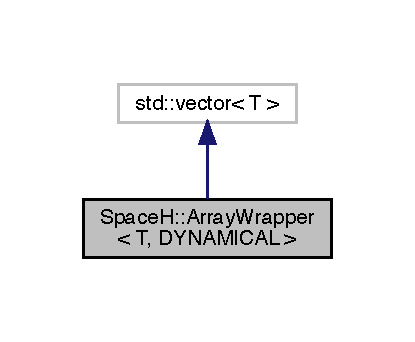
\includegraphics[width=199pt]{struct_space_h_1_1_array_wrapper_3_01_t_00_01_d_y_n_a_m_i_c_a_l_01_4__inherit__graph}
\end{center}
\end{figure}


Collaboration diagram for SpaceH\+:\+:Array\+Wrapper$<$ T, D\+Y\+N\+A\+M\+I\+C\+AL $>$\+:\nopagebreak
\begin{figure}[H]
\begin{center}
\leavevmode
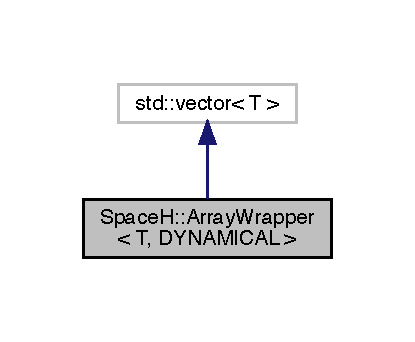
\includegraphics[width=199pt]{struct_space_h_1_1_array_wrapper_3_01_t_00_01_d_y_n_a_m_i_c_a_l_01_4__coll__graph}
\end{center}
\end{figure}


The documentation for this struct was generated from the following file\+:\begin{DoxyCompactItemize}
\item 
\mbox{\hyperlink{proto_type_8h}{proto\+Type.\+h}}\end{DoxyCompactItemize}

\hypertarget{class_b_s_iterator}{}\subsection{B\+S\+Iterator$<$ Partic\+Sys, Integrator $>$ Class Template Reference}
\label{class_b_s_iterator}\index{B\+S\+Iterator$<$ Partic\+Sys, Integrator $>$@{B\+S\+Iterator$<$ Partic\+Sys, Integrator $>$}}


Bulirsch-\/\+Stoer extrapolation algorithm.  




{\ttfamily \#include $<$B\+S\+Iterator.\+h$>$}

\subsubsection*{Public Types}
\begin{DoxyCompactItemize}
\item 
typedef Partic\+Sys\+::\+Scalar \mbox{\hyperlink{class_b_s_iterator_a7857f8ff9032955ea4dcc22cd18ca7a1}{Scalar}}
\item 
{\footnotesize template$<$typename Scalar , size\+\_\+t N$>$ }\\using \mbox{\hyperlink{class_b_s_iterator_ab0aa7c10b56500273af05dcd85fd8389}{scalar\+Array}} = std\+::array$<$ \mbox{\hyperlink{class_b_s_iterator_a7857f8ff9032955ea4dcc22cd18ca7a1}{Scalar}}, N $>$
\end{DoxyCompactItemize}
\subsubsection*{Public Member Functions}
\begin{DoxyCompactItemize}
\item 
\mbox{\hyperlink{class_b_s_iterator_a144fb5c55fcd7bc873e73f4d06276fb2}{B\+S\+Iterator}} ()
\begin{DoxyCompactList}\small\item\em Constructor for initializing cost, n\+Steps, fmin and CC. \end{DoxyCompactList}\item 
\mbox{\hyperlink{class_b_s_iterator_a7857f8ff9032955ea4dcc22cd18ca7a1}{Scalar}} \mbox{\hyperlink{class_b_s_iterator_a5520642ecbd454fb1f4d9ece18dc4e3f}{iterate}} (Partic\+Sys \&particles, Integrator \&integrator, \mbox{\hyperlink{class_b_s_iterator_a7857f8ff9032955ea4dcc22cd18ca7a1}{Scalar}} step\+Length)
\begin{DoxyCompactList}\small\item\em Interface of O\+DE iterator. \end{DoxyCompactList}\item 
void \mbox{\hyperlink{class_b_s_iterator_ada9b6cc673e297135646699d581fcdc7}{set\+Relative\+Error}} (\mbox{\hyperlink{class_b_s_iterator_a7857f8ff9032955ea4dcc22cd18ca7a1}{Scalar}} rel\+Error)
\begin{DoxyCompactList}\small\item\em Set the local relative error. \end{DoxyCompactList}\item 
void \mbox{\hyperlink{class_b_s_iterator_a57603539823be271c2229d0951b7d957}{set\+Absolute\+Error}} (\mbox{\hyperlink{class_b_s_iterator_a7857f8ff9032955ea4dcc22cd18ca7a1}{Scalar}} abs\+Error)
\begin{DoxyCompactList}\small\item\em Set the local absolute error. \end{DoxyCompactList}\end{DoxyCompactItemize}
\subsubsection*{Private Member Functions}
\begin{DoxyCompactItemize}
\item 
void \mbox{\hyperlink{class_b_s_iterator_a95c268219a8321af35a628db4e22bec4}{copy\+Data\+To\+Extrap\+Tab}} (size\+\_\+t k)
\begin{DoxyCompactList}\small\item\em Copy the current results of localsystem as a plain array to the first column of extrapolation talbe. \end{DoxyCompactList}\item 
bool \mbox{\hyperlink{class_b_s_iterator_a42976d786ffe422a86cc5a7b0a077609}{check\+Rejection}} (\mbox{\hyperlink{class_b_s_iterator_a7857f8ff9032955ea4dcc22cd18ca7a1}{Scalar}} error, size\+\_\+t k) const
\begin{DoxyCompactList}\small\item\em Check the rejection criteria for current iteration. \end{DoxyCompactList}\item 
void \mbox{\hyperlink{class_b_s_iterator_ac1edf158e3dd05ed15afd5d0f31c121a}{extrapolate}} (size\+\_\+t k)
\begin{DoxyCompactList}\small\item\em Extrapolate the kth row to the right end. \end{DoxyCompactList}\item 
\mbox{\hyperlink{class_b_s_iterator_a7857f8ff9032955ea4dcc22cd18ca7a1}{Scalar}} \mbox{\hyperlink{class_b_s_iterator_a9f50e084f8650e4d7fea3535a0547139}{get\+Error}} (size\+\_\+t k) const
\begin{DoxyCompactList}\small\item\em Calculate the error of the k row of the extrapolation table. \end{DoxyCompactList}\item 
\mbox{\hyperlink{class_b_s_iterator_a7857f8ff9032955ea4dcc22cd18ca7a1}{Scalar}} \mbox{\hyperlink{class_b_s_iterator_a9d06a0d0c9e458ea96952b0514adece9}{get\+Time\+Step\+Coef}} (\mbox{\hyperlink{class_b_s_iterator_a7857f8ff9032955ea4dcc22cd18ca7a1}{Scalar}} error, size\+\_\+t order)
\begin{DoxyCompactList}\small\item\em Calculate the new iteration integration step coefficient. \end{DoxyCompactList}\item 
\mbox{\hyperlink{class_b_s_iterator_a7857f8ff9032955ea4dcc22cd18ca7a1}{Scalar}} \mbox{\hyperlink{class_b_s_iterator_a738a558ddfacd9959c9438862001d7e8}{prepare\+For\+New\+Iteration}} (size\+\_\+t k, bool last\+Rejection)
\begin{DoxyCompactList}\small\item\em Calculate the new iteration integration step and new iteration depth for next iteration. \end{DoxyCompactList}\end{DoxyCompactItemize}
\subsubsection*{Private Attributes}
\begin{DoxyCompactItemize}
\item 
Partic\+Sys \mbox{\hyperlink{class_b_s_iterator_a9d6fc5f237246465161ea86854985395}{local\+System}}
\begin{DoxyCompactList}\small\item\em The local partical system used to iterate. \end{DoxyCompactList}\item 
\mbox{\hyperlink{class_b_s_iterator_ab0aa7c10b56500273af05dcd85fd8389}{scalar\+Array}}$<$ \mbox{\hyperlink{class_b_s_iterator_ab0aa7c10b56500273af05dcd85fd8389}{scalar\+Array}}$<$ \mbox{\hyperlink{class_b_s_iterator_a7857f8ff9032955ea4dcc22cd18ca7a1}{Scalar}}, Partic\+Sys\+::volume()$>$,(\mbox{\hyperlink{class_b_s_iterator_a39409b9a12d4854d101ce59a0efc0f74}{Max\+Depth}}+1) $\ast$(\mbox{\hyperlink{class_b_s_iterator_a39409b9a12d4854d101ce59a0efc0f74}{Max\+Depth}}+2)/2 $>$ \mbox{\hyperlink{class_b_s_iterator_aa501e973f342248fc445d59a5166ccc9}{extrap\+Tab}}
\begin{DoxyCompactList}\small\item\em Extrapolation table. \end{DoxyCompactList}\item 
\mbox{\hyperlink{class_b_s_iterator_ab0aa7c10b56500273af05dcd85fd8389}{scalar\+Array}}$<$ \mbox{\hyperlink{class_b_s_iterator_a7857f8ff9032955ea4dcc22cd18ca7a1}{Scalar}},(\mbox{\hyperlink{class_b_s_iterator_a39409b9a12d4854d101ce59a0efc0f74}{Max\+Depth}}+1) $\ast$(\mbox{\hyperlink{class_b_s_iterator_a39409b9a12d4854d101ce59a0efc0f74}{Max\+Depth}}+2)/2 $>$ \mbox{\hyperlink{class_b_s_iterator_a28f6cc2fd6bfd554f85225492f4210b7}{CC}}
\begin{DoxyCompactList}\small\item\em Extrapolation coefficient. \end{DoxyCompactList}\item 
\mbox{\hyperlink{class_b_s_iterator_ab0aa7c10b56500273af05dcd85fd8389}{scalar\+Array}}$<$ \mbox{\hyperlink{class_b_s_iterator_a7857f8ff9032955ea4dcc22cd18ca7a1}{Scalar}}, \mbox{\hyperlink{class_b_s_iterator_a39409b9a12d4854d101ce59a0efc0f74}{Max\+Depth}}+1 $>$ \mbox{\hyperlink{class_b_s_iterator_a96c58777cbefe7d02e160317621fc0b9}{macro\+Step\+Length}}
\begin{DoxyCompactList}\small\item\em Macro step length for different iteration depth. \end{DoxyCompactList}\item 
\mbox{\hyperlink{class_b_s_iterator_ab0aa7c10b56500273af05dcd85fd8389}{scalar\+Array}}$<$ \mbox{\hyperlink{class_b_s_iterator_a7857f8ff9032955ea4dcc22cd18ca7a1}{Scalar}}, \mbox{\hyperlink{class_b_s_iterator_a39409b9a12d4854d101ce59a0efc0f74}{Max\+Depth}}+1 $>$ \mbox{\hyperlink{class_b_s_iterator_ac2a338d6c3e5014d529666032d34c987}{work}}
\begin{DoxyCompactList}\small\item\em The work(calculation quantities) per integration length of each iteration depth. \end{DoxyCompactList}\item 
\mbox{\hyperlink{class_b_s_iterator_ab0aa7c10b56500273af05dcd85fd8389}{scalar\+Array}}$<$ \mbox{\hyperlink{class_b_s_iterator_a7857f8ff9032955ea4dcc22cd18ca7a1}{Scalar}}, \mbox{\hyperlink{class_b_s_iterator_a39409b9a12d4854d101ce59a0efc0f74}{Max\+Depth}}+1 $>$ \mbox{\hyperlink{class_b_s_iterator_a05bf5c727d23e47349683cda1a08ed13}{fmin}}
\begin{DoxyCompactList}\small\item\em The minimal coeffient of integration step estimation. \end{DoxyCompactList}\item 
\mbox{\hyperlink{class_b_s_iterator_ab0aa7c10b56500273af05dcd85fd8389}{scalar\+Array}}$<$ size\+\_\+t, \mbox{\hyperlink{class_b_s_iterator_a39409b9a12d4854d101ce59a0efc0f74}{Max\+Depth}}+1 $>$ \mbox{\hyperlink{class_b_s_iterator_a53f435811c23c0ae1713df13197fc9c9}{cost}}
\begin{DoxyCompactList}\small\item\em The work(calculation quantities) of each iteration depth. \end{DoxyCompactList}\item 
\mbox{\hyperlink{class_b_s_iterator_ab0aa7c10b56500273af05dcd85fd8389}{scalar\+Array}}$<$ size\+\_\+t, \mbox{\hyperlink{class_b_s_iterator_a39409b9a12d4854d101ce59a0efc0f74}{Max\+Depth}}+1 $>$ \mbox{\hyperlink{class_b_s_iterator_a9c4c8c17a759cdff694e0bd62ed249bd}{n\+Steps}}
\begin{DoxyCompactList}\small\item\em Steps of integration of each iteration depth. \end{DoxyCompactList}\item 
\mbox{\hyperlink{class_b_s_iterator_a7857f8ff9032955ea4dcc22cd18ca7a1}{Scalar}} \mbox{\hyperlink{class_b_s_iterator_a8948aa04b0ec390d43eb3d1f0a2efb03}{absolute\+Error}} \{1e-\/15\}
\begin{DoxyCompactList}\small\item\em Local absolute error. \end{DoxyCompactList}\item 
\mbox{\hyperlink{class_b_s_iterator_a7857f8ff9032955ea4dcc22cd18ca7a1}{Scalar}} \mbox{\hyperlink{class_b_s_iterator_abce71b7bac10363f7772dc848f8722b6}{relative\+Error}} \{1e-\/15\}
\begin{DoxyCompactList}\small\item\em Local relative error. \end{DoxyCompactList}\item 
\mbox{\hyperlink{class_b_s_iterator_a7857f8ff9032955ea4dcc22cd18ca7a1}{Scalar}} \mbox{\hyperlink{class_b_s_iterator_a942f85e00c28ef1990d1dfbed69c9e13}{s1}} \{0.\+94\}
\begin{DoxyCompactList}\small\item\em Coefficient of new step length estimation. See \char`\"{}\+Numerical recipes\char`\"{} on page 926. \end{DoxyCompactList}\item 
\mbox{\hyperlink{class_b_s_iterator_a7857f8ff9032955ea4dcc22cd18ca7a1}{Scalar}} \mbox{\hyperlink{class_b_s_iterator_ad1cdde25df6bca7a456c1908be54065f}{s2}} \{0.\+95\}
\begin{DoxyCompactList}\small\item\em Coefficient of new step length estimation. \end{DoxyCompactList}\item 
\mbox{\hyperlink{class_b_s_iterator_a7857f8ff9032955ea4dcc22cd18ca7a1}{Scalar}} \mbox{\hyperlink{class_b_s_iterator_a10ea0bb96f7971e9c477daef1fda6e16}{s3}} \{0.\+02\}
\begin{DoxyCompactList}\small\item\em Coefficient of new step length estimation. \end{DoxyCompactList}\item 
\mbox{\hyperlink{class_b_s_iterator_a7857f8ff9032955ea4dcc22cd18ca7a1}{Scalar}} \mbox{\hyperlink{class_b_s_iterator_a5b3bbb2d988a5d91030060508e3b4f66}{s4}} \{4.\+0\}
\begin{DoxyCompactList}\small\item\em Coefficient of new step length estimation. \end{DoxyCompactList}\item 
size\+\_\+t \mbox{\hyperlink{class_b_s_iterator_aa073f847cc5855f727c8f326f539a5f0}{iter\+Depth}} \{7\}
\begin{DoxyCompactList}\small\item\em Current iteraation depth. \end{DoxyCompactList}\end{DoxyCompactItemize}
\subsubsection*{Static Private Attributes}
\begin{DoxyCompactItemize}
\item 
static const size\+\_\+t \mbox{\hyperlink{class_b_s_iterator_a39409b9a12d4854d101ce59a0efc0f74}{Max\+Depth}} \{8\}
\begin{DoxyCompactList}\small\item\em The Maximum iteration depth. \end{DoxyCompactList}\end{DoxyCompactItemize}


\subsubsection{Detailed Description}
\subsubsection*{template$<$typename Partic\+Sys, typename Integrator$>$\newline
class B\+S\+Iterator$<$ Partic\+Sys, Integrator $>$}

Bulirsch-\/\+Stoer extrapolation algorithm. 

\subsubsection{Member Typedef Documentation}
\mbox{\Hypertarget{class_b_s_iterator_a7857f8ff9032955ea4dcc22cd18ca7a1}\label{class_b_s_iterator_a7857f8ff9032955ea4dcc22cd18ca7a1}} 
\index{B\+S\+Iterator@{B\+S\+Iterator}!Scalar@{Scalar}}
\index{Scalar@{Scalar}!B\+S\+Iterator@{B\+S\+Iterator}}
\paragraph{\texorpdfstring{Scalar}{Scalar}}
{\footnotesize\ttfamily template$<$typename Partic\+Sys , typename Integrator $>$ \\
typedef Partic\+Sys\+::\+Scalar \mbox{\hyperlink{class_b_s_iterator}{B\+S\+Iterator}}$<$ Partic\+Sys, Integrator $>$\+::\mbox{\hyperlink{class_b_s_iterator_a7857f8ff9032955ea4dcc22cd18ca7a1}{Scalar}}}

\mbox{\Hypertarget{class_b_s_iterator_ab0aa7c10b56500273af05dcd85fd8389}\label{class_b_s_iterator_ab0aa7c10b56500273af05dcd85fd8389}} 
\index{B\+S\+Iterator@{B\+S\+Iterator}!scalar\+Array@{scalar\+Array}}
\index{scalar\+Array@{scalar\+Array}!B\+S\+Iterator@{B\+S\+Iterator}}
\paragraph{\texorpdfstring{scalar\+Array}{scalarArray}}
{\footnotesize\ttfamily template$<$typename Partic\+Sys , typename Integrator $>$ \\
template$<$typename Scalar , size\+\_\+t N$>$ \\
using \mbox{\hyperlink{class_b_s_iterator}{B\+S\+Iterator}}$<$ Partic\+Sys, Integrator $>$\+::\mbox{\hyperlink{class_b_s_iterator_ab0aa7c10b56500273af05dcd85fd8389}{scalar\+Array}} =  std\+::array$<$\mbox{\hyperlink{class_b_s_iterator_a7857f8ff9032955ea4dcc22cd18ca7a1}{Scalar}}, N$>$}



\subsubsection{Constructor \& Destructor Documentation}
\mbox{\Hypertarget{class_b_s_iterator_a144fb5c55fcd7bc873e73f4d06276fb2}\label{class_b_s_iterator_a144fb5c55fcd7bc873e73f4d06276fb2}} 
\index{B\+S\+Iterator@{B\+S\+Iterator}!B\+S\+Iterator@{B\+S\+Iterator}}
\index{B\+S\+Iterator@{B\+S\+Iterator}!B\+S\+Iterator@{B\+S\+Iterator}}
\paragraph{\texorpdfstring{B\+S\+Iterator()}{BSIterator()}}
{\footnotesize\ttfamily template$<$typename Partic\+Sys , typename Integrator $>$ \\
\mbox{\hyperlink{class_b_s_iterator}{B\+S\+Iterator}}$<$ Partic\+Sys, Integrator $>$\+::\mbox{\hyperlink{class_b_s_iterator}{B\+S\+Iterator}} (\begin{DoxyParamCaption}{ }\end{DoxyParamCaption})}



Constructor for initializing cost, n\+Steps, fmin and CC. 



\subsubsection{Member Function Documentation}
\mbox{\Hypertarget{class_b_s_iterator_a42976d786ffe422a86cc5a7b0a077609}\label{class_b_s_iterator_a42976d786ffe422a86cc5a7b0a077609}} 
\index{B\+S\+Iterator@{B\+S\+Iterator}!check\+Rejection@{check\+Rejection}}
\index{check\+Rejection@{check\+Rejection}!B\+S\+Iterator@{B\+S\+Iterator}}
\paragraph{\texorpdfstring{check\+Rejection()}{checkRejection()}}
{\footnotesize\ttfamily template$<$typename Partic\+Sys , typename Integrator $>$ \\
bool \mbox{\hyperlink{class_b_s_iterator}{B\+S\+Iterator}}$<$ Partic\+Sys, Integrator $>$\+::check\+Rejection (\begin{DoxyParamCaption}\item[{\mbox{\hyperlink{class_b_s_iterator_a7857f8ff9032955ea4dcc22cd18ca7a1}{Scalar}}}]{error,  }\item[{size\+\_\+t}]{k }\end{DoxyParamCaption}) const\hspace{0.3cm}{\ttfamily [private]}}



Check the rejection criteria for current iteration. 


\begin{DoxyParams}{Parameters}
{\em k} & The kth iteration depth. \\
\hline
\end{DoxyParams}
\begin{DoxyReturn}{Returns}
If current iteration is rejected. 
\end{DoxyReturn}
\mbox{\Hypertarget{class_b_s_iterator_a95c268219a8321af35a628db4e22bec4}\label{class_b_s_iterator_a95c268219a8321af35a628db4e22bec4}} 
\index{B\+S\+Iterator@{B\+S\+Iterator}!copy\+Data\+To\+Extrap\+Tab@{copy\+Data\+To\+Extrap\+Tab}}
\index{copy\+Data\+To\+Extrap\+Tab@{copy\+Data\+To\+Extrap\+Tab}!B\+S\+Iterator@{B\+S\+Iterator}}
\paragraph{\texorpdfstring{copy\+Data\+To\+Extrap\+Tab()}{copyDataToExtrapTab()}}
{\footnotesize\ttfamily template$<$typename Partic\+Sys , typename Integrator $>$ \\
void \mbox{\hyperlink{class_b_s_iterator}{B\+S\+Iterator}}$<$ Partic\+Sys, Integrator $>$\+::copy\+Data\+To\+Extrap\+Tab (\begin{DoxyParamCaption}\item[{size\+\_\+t}]{k }\end{DoxyParamCaption})\hspace{0.3cm}{\ttfamily [private]}}



Copy the current results of localsystem as a plain array to the first column of extrapolation talbe. 


\begin{DoxyParams}{Parameters}
{\em k} & The kth row of extrapolation table. \\
\hline
\end{DoxyParams}
\mbox{\Hypertarget{class_b_s_iterator_ac1edf158e3dd05ed15afd5d0f31c121a}\label{class_b_s_iterator_ac1edf158e3dd05ed15afd5d0f31c121a}} 
\index{B\+S\+Iterator@{B\+S\+Iterator}!extrapolate@{extrapolate}}
\index{extrapolate@{extrapolate}!B\+S\+Iterator@{B\+S\+Iterator}}
\paragraph{\texorpdfstring{extrapolate()}{extrapolate()}}
{\footnotesize\ttfamily template$<$typename Partic\+Sys , typename Integrator $>$ \\
void \mbox{\hyperlink{class_b_s_iterator}{B\+S\+Iterator}}$<$ Partic\+Sys, Integrator $>$\+::extrapolate (\begin{DoxyParamCaption}\item[{size\+\_\+t}]{k }\end{DoxyParamCaption})\hspace{0.3cm}{\ttfamily [private]}}



Extrapolate the kth row to the right end. 

Extrapolate the k-\/th row to the right end.


\begin{DoxyParams}{Parameters}
{\em k} & The kth row of extrapolation table. \\
\hline
\end{DoxyParams}
\mbox{\Hypertarget{class_b_s_iterator_a9f50e084f8650e4d7fea3535a0547139}\label{class_b_s_iterator_a9f50e084f8650e4d7fea3535a0547139}} 
\index{B\+S\+Iterator@{B\+S\+Iterator}!get\+Error@{get\+Error}}
\index{get\+Error@{get\+Error}!B\+S\+Iterator@{B\+S\+Iterator}}
\paragraph{\texorpdfstring{get\+Error()}{getError()}}
{\footnotesize\ttfamily template$<$typename Partic\+Sys , typename Integrator $>$ \\
Partic\+Sys\+::\+Scalar \mbox{\hyperlink{class_b_s_iterator}{B\+S\+Iterator}}$<$ Partic\+Sys, Integrator $>$\+::get\+Error (\begin{DoxyParamCaption}\item[{size\+\_\+t}]{k }\end{DoxyParamCaption}) const\hspace{0.3cm}{\ttfamily [private]}}



Calculate the error of the k row of the extrapolation table. 


\begin{DoxyParams}{Parameters}
{\em k} & The kth row of extrapolation table. \\
\hline
\end{DoxyParams}
Here is the call graph for this function\+:\nopagebreak
\begin{figure}[H]
\begin{center}
\leavevmode
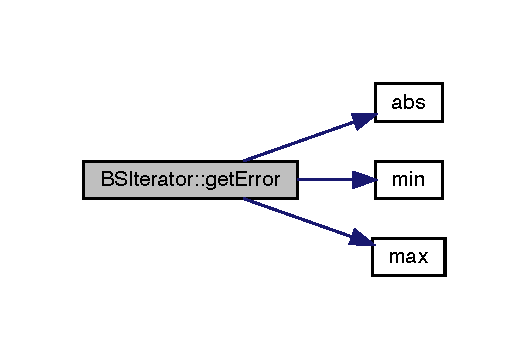
\includegraphics[width=254pt]{class_b_s_iterator_a9f50e084f8650e4d7fea3535a0547139_cgraph}
\end{center}
\end{figure}
\mbox{\Hypertarget{class_b_s_iterator_a9d06a0d0c9e458ea96952b0514adece9}\label{class_b_s_iterator_a9d06a0d0c9e458ea96952b0514adece9}} 
\index{B\+S\+Iterator@{B\+S\+Iterator}!get\+Time\+Step\+Coef@{get\+Time\+Step\+Coef}}
\index{get\+Time\+Step\+Coef@{get\+Time\+Step\+Coef}!B\+S\+Iterator@{B\+S\+Iterator}}
\paragraph{\texorpdfstring{get\+Time\+Step\+Coef()}{getTimeStepCoef()}}
{\footnotesize\ttfamily template$<$typename Partic\+Sys , typename Integrator $>$ \\
Partic\+Sys\+::\+Scalar \mbox{\hyperlink{class_b_s_iterator}{B\+S\+Iterator}}$<$ Partic\+Sys, Integrator $>$\+::get\+Time\+Step\+Coef (\begin{DoxyParamCaption}\item[{\mbox{\hyperlink{class_b_s_iterator_a7857f8ff9032955ea4dcc22cd18ca7a1}{Scalar}}}]{error,  }\item[{size\+\_\+t}]{order }\end{DoxyParamCaption})\hspace{0.3cm}{\ttfamily [private]}}



Calculate the new iteration integration step coefficient. 


\begin{DoxyParams}{Parameters}
{\em error} & The error of the k-\/th row of extrapolation table. \\
\hline
{\em order} & The order of the error in k-\/th row of extrapolation table. \\
\hline
\end{DoxyParams}
\begin{DoxyReturn}{Returns}
The new iteration integration step length coefficient. 
\end{DoxyReturn}
Here is the call graph for this function\+:\nopagebreak
\begin{figure}[H]
\begin{center}
\leavevmode
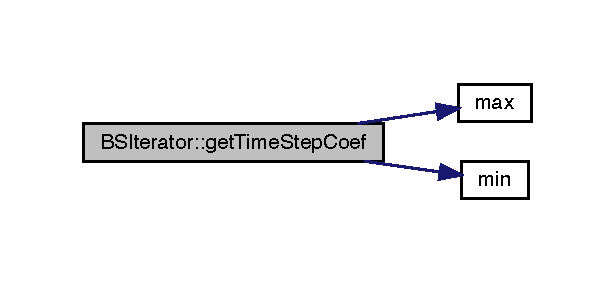
\includegraphics[width=295pt]{class_b_s_iterator_a9d06a0d0c9e458ea96952b0514adece9_cgraph}
\end{center}
\end{figure}
\mbox{\Hypertarget{class_b_s_iterator_a5520642ecbd454fb1f4d9ece18dc4e3f}\label{class_b_s_iterator_a5520642ecbd454fb1f4d9ece18dc4e3f}} 
\index{B\+S\+Iterator@{B\+S\+Iterator}!iterate@{iterate}}
\index{iterate@{iterate}!B\+S\+Iterator@{B\+S\+Iterator}}
\paragraph{\texorpdfstring{iterate()}{iterate()}}
{\footnotesize\ttfamily template$<$typename Partic\+Sys , typename Integrator $>$ \\
Partic\+Sys\+::\+Scalar \mbox{\hyperlink{class_b_s_iterator}{B\+S\+Iterator}}$<$ Partic\+Sys, Integrator $>$\+::iterate (\begin{DoxyParamCaption}\item[{Partic\+Sys \&}]{particles,  }\item[{Integrator \&}]{integrator,  }\item[{\mbox{\hyperlink{class_b_s_iterator_a7857f8ff9032955ea4dcc22cd18ca7a1}{Scalar}}}]{step\+Length }\end{DoxyParamCaption})}



Interface of O\+DE iterator. 

\begin{DoxyNote}{Note}
B\+Siterator will force use the internal mid-\/point integrator as the basic integrator.
\end{DoxyNote}

\begin{DoxyParams}{Parameters}
{\em particles} & Particle system need iteration. \\
\hline
{\em integrator} & Basica integrator used to evolve, but here BS iterator will force use internal mid-\/point integrator. \\
\hline
{\em step\+Length} & Macro integration step length. \\
\hline
\end{DoxyParams}
\begin{DoxyReturn}{Returns}
The next macro integration step length. 
\end{DoxyReturn}
\mbox{\Hypertarget{class_b_s_iterator_a738a558ddfacd9959c9438862001d7e8}\label{class_b_s_iterator_a738a558ddfacd9959c9438862001d7e8}} 
\index{B\+S\+Iterator@{B\+S\+Iterator}!prepare\+For\+New\+Iteration@{prepare\+For\+New\+Iteration}}
\index{prepare\+For\+New\+Iteration@{prepare\+For\+New\+Iteration}!B\+S\+Iterator@{B\+S\+Iterator}}
\paragraph{\texorpdfstring{prepare\+For\+New\+Iteration()}{prepareForNewIteration()}}
{\footnotesize\ttfamily template$<$typename Partic\+Sys , typename Integrator $>$ \\
Partic\+Sys\+::\+Scalar \mbox{\hyperlink{class_b_s_iterator}{B\+S\+Iterator}}$<$ Partic\+Sys, Integrator $>$\+::prepare\+For\+New\+Iteration (\begin{DoxyParamCaption}\item[{size\+\_\+t}]{k,  }\item[{bool}]{last\+Rejection }\end{DoxyParamCaption})\hspace{0.3cm}{\ttfamily [private]}}



Calculate the new iteration integration step and new iteration depth for next iteration. 


\begin{DoxyParams}{Parameters}
{\em k} & The k-\/th iteration depth. \\
\hline
{\em last\+Rejection} & The rejection status of last trail of iteration. \\
\hline
\end{DoxyParams}
\begin{DoxyReturn}{Returns}
The new iteration step length. 
\end{DoxyReturn}
Here is the call graph for this function\+:\nopagebreak
\begin{figure}[H]
\begin{center}
\leavevmode
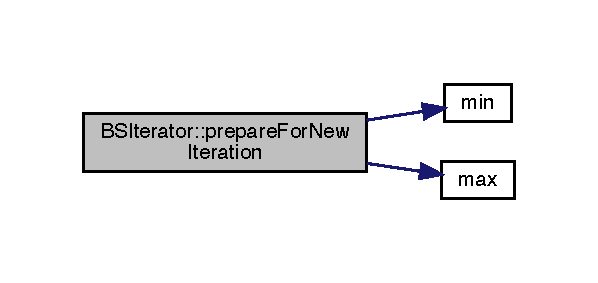
\includegraphics[width=287pt]{class_b_s_iterator_a738a558ddfacd9959c9438862001d7e8_cgraph}
\end{center}
\end{figure}
\mbox{\Hypertarget{class_b_s_iterator_a57603539823be271c2229d0951b7d957}\label{class_b_s_iterator_a57603539823be271c2229d0951b7d957}} 
\index{B\+S\+Iterator@{B\+S\+Iterator}!set\+Absolute\+Error@{set\+Absolute\+Error}}
\index{set\+Absolute\+Error@{set\+Absolute\+Error}!B\+S\+Iterator@{B\+S\+Iterator}}
\paragraph{\texorpdfstring{set\+Absolute\+Error()}{setAbsoluteError()}}
{\footnotesize\ttfamily template$<$typename Partic\+Sys , typename Integrator $>$ \\
void \mbox{\hyperlink{class_b_s_iterator}{B\+S\+Iterator}}$<$ Partic\+Sys, Integrator $>$\+::set\+Absolute\+Error (\begin{DoxyParamCaption}\item[{\mbox{\hyperlink{class_b_s_iterator_a7857f8ff9032955ea4dcc22cd18ca7a1}{Scalar}}}]{abs\+Error }\end{DoxyParamCaption})\hspace{0.3cm}{\ttfamily [inline]}}



Set the local absolute error. 

\mbox{\Hypertarget{class_b_s_iterator_ada9b6cc673e297135646699d581fcdc7}\label{class_b_s_iterator_ada9b6cc673e297135646699d581fcdc7}} 
\index{B\+S\+Iterator@{B\+S\+Iterator}!set\+Relative\+Error@{set\+Relative\+Error}}
\index{set\+Relative\+Error@{set\+Relative\+Error}!B\+S\+Iterator@{B\+S\+Iterator}}
\paragraph{\texorpdfstring{set\+Relative\+Error()}{setRelativeError()}}
{\footnotesize\ttfamily template$<$typename Partic\+Sys , typename Integrator $>$ \\
void \mbox{\hyperlink{class_b_s_iterator}{B\+S\+Iterator}}$<$ Partic\+Sys, Integrator $>$\+::set\+Relative\+Error (\begin{DoxyParamCaption}\item[{\mbox{\hyperlink{class_b_s_iterator_a7857f8ff9032955ea4dcc22cd18ca7a1}{Scalar}}}]{rel\+Error }\end{DoxyParamCaption})\hspace{0.3cm}{\ttfamily [inline]}}



Set the local relative error. 



\subsubsection{Member Data Documentation}
\mbox{\Hypertarget{class_b_s_iterator_a8948aa04b0ec390d43eb3d1f0a2efb03}\label{class_b_s_iterator_a8948aa04b0ec390d43eb3d1f0a2efb03}} 
\index{B\+S\+Iterator@{B\+S\+Iterator}!absolute\+Error@{absolute\+Error}}
\index{absolute\+Error@{absolute\+Error}!B\+S\+Iterator@{B\+S\+Iterator}}
\paragraph{\texorpdfstring{absolute\+Error}{absoluteError}}
{\footnotesize\ttfamily template$<$typename Partic\+Sys , typename Integrator $>$ \\
\mbox{\hyperlink{class_b_s_iterator_a7857f8ff9032955ea4dcc22cd18ca7a1}{Scalar}} \mbox{\hyperlink{class_b_s_iterator}{B\+S\+Iterator}}$<$ Partic\+Sys, Integrator $>$\+::absolute\+Error \{1e-\/15\}\hspace{0.3cm}{\ttfamily [private]}}



Local absolute error. 

\mbox{\Hypertarget{class_b_s_iterator_a28f6cc2fd6bfd554f85225492f4210b7}\label{class_b_s_iterator_a28f6cc2fd6bfd554f85225492f4210b7}} 
\index{B\+S\+Iterator@{B\+S\+Iterator}!CC@{CC}}
\index{CC@{CC}!B\+S\+Iterator@{B\+S\+Iterator}}
\paragraph{\texorpdfstring{CC}{CC}}
{\footnotesize\ttfamily template$<$typename Partic\+Sys , typename Integrator $>$ \\
\mbox{\hyperlink{class_b_s_iterator_ab0aa7c10b56500273af05dcd85fd8389}{scalar\+Array}}$<$ \mbox{\hyperlink{class_b_s_iterator_a7857f8ff9032955ea4dcc22cd18ca7a1}{Scalar}}, (\mbox{\hyperlink{class_b_s_iterator_a39409b9a12d4854d101ce59a0efc0f74}{Max\+Depth}} + 1)$\ast$ (\mbox{\hyperlink{class_b_s_iterator_a39409b9a12d4854d101ce59a0efc0f74}{Max\+Depth}} + 2) / 2 $>$ \mbox{\hyperlink{class_b_s_iterator}{B\+S\+Iterator}}$<$ Partic\+Sys, Integrator $>$\+::CC\hspace{0.3cm}{\ttfamily [private]}}



Extrapolation coefficient. 

\mbox{\Hypertarget{class_b_s_iterator_a53f435811c23c0ae1713df13197fc9c9}\label{class_b_s_iterator_a53f435811c23c0ae1713df13197fc9c9}} 
\index{B\+S\+Iterator@{B\+S\+Iterator}!cost@{cost}}
\index{cost@{cost}!B\+S\+Iterator@{B\+S\+Iterator}}
\paragraph{\texorpdfstring{cost}{cost}}
{\footnotesize\ttfamily template$<$typename Partic\+Sys , typename Integrator $>$ \\
\mbox{\hyperlink{class_b_s_iterator_ab0aa7c10b56500273af05dcd85fd8389}{scalar\+Array}}$<$ size\+\_\+t, \mbox{\hyperlink{class_b_s_iterator_a39409b9a12d4854d101ce59a0efc0f74}{Max\+Depth}} + 1 $>$ \mbox{\hyperlink{class_b_s_iterator}{B\+S\+Iterator}}$<$ Partic\+Sys, Integrator $>$\+::cost\hspace{0.3cm}{\ttfamily [private]}}



The work(calculation quantities) of each iteration depth. 

\mbox{\Hypertarget{class_b_s_iterator_aa501e973f342248fc445d59a5166ccc9}\label{class_b_s_iterator_aa501e973f342248fc445d59a5166ccc9}} 
\index{B\+S\+Iterator@{B\+S\+Iterator}!extrap\+Tab@{extrap\+Tab}}
\index{extrap\+Tab@{extrap\+Tab}!B\+S\+Iterator@{B\+S\+Iterator}}
\paragraph{\texorpdfstring{extrap\+Tab}{extrapTab}}
{\footnotesize\ttfamily template$<$typename Partic\+Sys , typename Integrator $>$ \\
\mbox{\hyperlink{class_b_s_iterator_ab0aa7c10b56500273af05dcd85fd8389}{scalar\+Array}}$<$ \mbox{\hyperlink{class_b_s_iterator_ab0aa7c10b56500273af05dcd85fd8389}{scalar\+Array}}$<$\mbox{\hyperlink{class_b_s_iterator_a7857f8ff9032955ea4dcc22cd18ca7a1}{Scalar}}, Partic\+Sys\+::volume()$>$, (\mbox{\hyperlink{class_b_s_iterator_a39409b9a12d4854d101ce59a0efc0f74}{Max\+Depth}} + 1)$\ast$ (\mbox{\hyperlink{class_b_s_iterator_a39409b9a12d4854d101ce59a0efc0f74}{Max\+Depth}} + 2) / 2 $>$ \mbox{\hyperlink{class_b_s_iterator}{B\+S\+Iterator}}$<$ Partic\+Sys, Integrator $>$\+::extrap\+Tab\hspace{0.3cm}{\ttfamily [private]}}



Extrapolation table. 

\mbox{\Hypertarget{class_b_s_iterator_a05bf5c727d23e47349683cda1a08ed13}\label{class_b_s_iterator_a05bf5c727d23e47349683cda1a08ed13}} 
\index{B\+S\+Iterator@{B\+S\+Iterator}!fmin@{fmin}}
\index{fmin@{fmin}!B\+S\+Iterator@{B\+S\+Iterator}}
\paragraph{\texorpdfstring{fmin}{fmin}}
{\footnotesize\ttfamily template$<$typename Partic\+Sys , typename Integrator $>$ \\
\mbox{\hyperlink{class_b_s_iterator_ab0aa7c10b56500273af05dcd85fd8389}{scalar\+Array}}$<$ \mbox{\hyperlink{class_b_s_iterator_a7857f8ff9032955ea4dcc22cd18ca7a1}{Scalar}}, \mbox{\hyperlink{class_b_s_iterator_a39409b9a12d4854d101ce59a0efc0f74}{Max\+Depth}} + 1 $>$ \mbox{\hyperlink{class_b_s_iterator}{B\+S\+Iterator}}$<$ Partic\+Sys, Integrator $>$\+::fmin\hspace{0.3cm}{\ttfamily [private]}}



The minimal coeffient of integration step estimation. 

\mbox{\Hypertarget{class_b_s_iterator_aa073f847cc5855f727c8f326f539a5f0}\label{class_b_s_iterator_aa073f847cc5855f727c8f326f539a5f0}} 
\index{B\+S\+Iterator@{B\+S\+Iterator}!iter\+Depth@{iter\+Depth}}
\index{iter\+Depth@{iter\+Depth}!B\+S\+Iterator@{B\+S\+Iterator}}
\paragraph{\texorpdfstring{iter\+Depth}{iterDepth}}
{\footnotesize\ttfamily template$<$typename Partic\+Sys , typename Integrator $>$ \\
size\+\_\+t \mbox{\hyperlink{class_b_s_iterator}{B\+S\+Iterator}}$<$ Partic\+Sys, Integrator $>$\+::iter\+Depth \{7\}\hspace{0.3cm}{\ttfamily [private]}}



Current iteraation depth. 

\mbox{\Hypertarget{class_b_s_iterator_a9d6fc5f237246465161ea86854985395}\label{class_b_s_iterator_a9d6fc5f237246465161ea86854985395}} 
\index{B\+S\+Iterator@{B\+S\+Iterator}!local\+System@{local\+System}}
\index{local\+System@{local\+System}!B\+S\+Iterator@{B\+S\+Iterator}}
\paragraph{\texorpdfstring{local\+System}{localSystem}}
{\footnotesize\ttfamily template$<$typename Partic\+Sys , typename Integrator $>$ \\
Partic\+Sys \mbox{\hyperlink{class_b_s_iterator}{B\+S\+Iterator}}$<$ Partic\+Sys, Integrator $>$\+::local\+System\hspace{0.3cm}{\ttfamily [private]}}



The local partical system used to iterate. 

\mbox{\Hypertarget{class_b_s_iterator_a96c58777cbefe7d02e160317621fc0b9}\label{class_b_s_iterator_a96c58777cbefe7d02e160317621fc0b9}} 
\index{B\+S\+Iterator@{B\+S\+Iterator}!macro\+Step\+Length@{macro\+Step\+Length}}
\index{macro\+Step\+Length@{macro\+Step\+Length}!B\+S\+Iterator@{B\+S\+Iterator}}
\paragraph{\texorpdfstring{macro\+Step\+Length}{macroStepLength}}
{\footnotesize\ttfamily template$<$typename Partic\+Sys , typename Integrator $>$ \\
\mbox{\hyperlink{class_b_s_iterator_ab0aa7c10b56500273af05dcd85fd8389}{scalar\+Array}}$<$ \mbox{\hyperlink{class_b_s_iterator_a7857f8ff9032955ea4dcc22cd18ca7a1}{Scalar}}, \mbox{\hyperlink{class_b_s_iterator_a39409b9a12d4854d101ce59a0efc0f74}{Max\+Depth}} + 1 $>$ \mbox{\hyperlink{class_b_s_iterator}{B\+S\+Iterator}}$<$ Partic\+Sys, Integrator $>$\+::macro\+Step\+Length\hspace{0.3cm}{\ttfamily [private]}}



Macro step length for different iteration depth. 

\mbox{\Hypertarget{class_b_s_iterator_a39409b9a12d4854d101ce59a0efc0f74}\label{class_b_s_iterator_a39409b9a12d4854d101ce59a0efc0f74}} 
\index{B\+S\+Iterator@{B\+S\+Iterator}!Max\+Depth@{Max\+Depth}}
\index{Max\+Depth@{Max\+Depth}!B\+S\+Iterator@{B\+S\+Iterator}}
\paragraph{\texorpdfstring{Max\+Depth}{MaxDepth}}
{\footnotesize\ttfamily template$<$typename Partic\+Sys , typename Integrator $>$ \\
const size\+\_\+t \mbox{\hyperlink{class_b_s_iterator}{B\+S\+Iterator}}$<$ Partic\+Sys, Integrator $>$\+::Max\+Depth \{8\}\hspace{0.3cm}{\ttfamily [static]}, {\ttfamily [private]}}



The Maximum iteration depth. 

\mbox{\Hypertarget{class_b_s_iterator_a9c4c8c17a759cdff694e0bd62ed249bd}\label{class_b_s_iterator_a9c4c8c17a759cdff694e0bd62ed249bd}} 
\index{B\+S\+Iterator@{B\+S\+Iterator}!n\+Steps@{n\+Steps}}
\index{n\+Steps@{n\+Steps}!B\+S\+Iterator@{B\+S\+Iterator}}
\paragraph{\texorpdfstring{n\+Steps}{nSteps}}
{\footnotesize\ttfamily template$<$typename Partic\+Sys , typename Integrator $>$ \\
\mbox{\hyperlink{class_b_s_iterator_ab0aa7c10b56500273af05dcd85fd8389}{scalar\+Array}}$<$ size\+\_\+t, \mbox{\hyperlink{class_b_s_iterator_a39409b9a12d4854d101ce59a0efc0f74}{Max\+Depth}} + 1 $>$ \mbox{\hyperlink{class_b_s_iterator}{B\+S\+Iterator}}$<$ Partic\+Sys, Integrator $>$\+::n\+Steps\hspace{0.3cm}{\ttfamily [private]}}



Steps of integration of each iteration depth. 

\mbox{\Hypertarget{class_b_s_iterator_abce71b7bac10363f7772dc848f8722b6}\label{class_b_s_iterator_abce71b7bac10363f7772dc848f8722b6}} 
\index{B\+S\+Iterator@{B\+S\+Iterator}!relative\+Error@{relative\+Error}}
\index{relative\+Error@{relative\+Error}!B\+S\+Iterator@{B\+S\+Iterator}}
\paragraph{\texorpdfstring{relative\+Error}{relativeError}}
{\footnotesize\ttfamily template$<$typename Partic\+Sys , typename Integrator $>$ \\
\mbox{\hyperlink{class_b_s_iterator_a7857f8ff9032955ea4dcc22cd18ca7a1}{Scalar}} \mbox{\hyperlink{class_b_s_iterator}{B\+S\+Iterator}}$<$ Partic\+Sys, Integrator $>$\+::relative\+Error \{1e-\/15\}\hspace{0.3cm}{\ttfamily [private]}}



Local relative error. 

\mbox{\Hypertarget{class_b_s_iterator_a942f85e00c28ef1990d1dfbed69c9e13}\label{class_b_s_iterator_a942f85e00c28ef1990d1dfbed69c9e13}} 
\index{B\+S\+Iterator@{B\+S\+Iterator}!s1@{s1}}
\index{s1@{s1}!B\+S\+Iterator@{B\+S\+Iterator}}
\paragraph{\texorpdfstring{s1}{s1}}
{\footnotesize\ttfamily template$<$typename Partic\+Sys , typename Integrator $>$ \\
\mbox{\hyperlink{class_b_s_iterator_a7857f8ff9032955ea4dcc22cd18ca7a1}{Scalar}} \mbox{\hyperlink{class_b_s_iterator}{B\+S\+Iterator}}$<$ Partic\+Sys, Integrator $>$\+::s1 \{0.\+94\}\hspace{0.3cm}{\ttfamily [private]}}



Coefficient of new step length estimation. See \char`\"{}\+Numerical recipes\char`\"{} on page 926. 

\mbox{\Hypertarget{class_b_s_iterator_ad1cdde25df6bca7a456c1908be54065f}\label{class_b_s_iterator_ad1cdde25df6bca7a456c1908be54065f}} 
\index{B\+S\+Iterator@{B\+S\+Iterator}!s2@{s2}}
\index{s2@{s2}!B\+S\+Iterator@{B\+S\+Iterator}}
\paragraph{\texorpdfstring{s2}{s2}}
{\footnotesize\ttfamily template$<$typename Partic\+Sys , typename Integrator $>$ \\
\mbox{\hyperlink{class_b_s_iterator_a7857f8ff9032955ea4dcc22cd18ca7a1}{Scalar}} \mbox{\hyperlink{class_b_s_iterator}{B\+S\+Iterator}}$<$ Partic\+Sys, Integrator $>$\+::s2 \{0.\+95\}\hspace{0.3cm}{\ttfamily [private]}}



Coefficient of new step length estimation. 

\mbox{\Hypertarget{class_b_s_iterator_a10ea0bb96f7971e9c477daef1fda6e16}\label{class_b_s_iterator_a10ea0bb96f7971e9c477daef1fda6e16}} 
\index{B\+S\+Iterator@{B\+S\+Iterator}!s3@{s3}}
\index{s3@{s3}!B\+S\+Iterator@{B\+S\+Iterator}}
\paragraph{\texorpdfstring{s3}{s3}}
{\footnotesize\ttfamily template$<$typename Partic\+Sys , typename Integrator $>$ \\
\mbox{\hyperlink{class_b_s_iterator_a7857f8ff9032955ea4dcc22cd18ca7a1}{Scalar}} \mbox{\hyperlink{class_b_s_iterator}{B\+S\+Iterator}}$<$ Partic\+Sys, Integrator $>$\+::s3 \{0.\+02\}\hspace{0.3cm}{\ttfamily [private]}}



Coefficient of new step length estimation. 

\mbox{\Hypertarget{class_b_s_iterator_a5b3bbb2d988a5d91030060508e3b4f66}\label{class_b_s_iterator_a5b3bbb2d988a5d91030060508e3b4f66}} 
\index{B\+S\+Iterator@{B\+S\+Iterator}!s4@{s4}}
\index{s4@{s4}!B\+S\+Iterator@{B\+S\+Iterator}}
\paragraph{\texorpdfstring{s4}{s4}}
{\footnotesize\ttfamily template$<$typename Partic\+Sys , typename Integrator $>$ \\
\mbox{\hyperlink{class_b_s_iterator_a7857f8ff9032955ea4dcc22cd18ca7a1}{Scalar}} \mbox{\hyperlink{class_b_s_iterator}{B\+S\+Iterator}}$<$ Partic\+Sys, Integrator $>$\+::s4 \{4.\+0\}\hspace{0.3cm}{\ttfamily [private]}}



Coefficient of new step length estimation. 

\mbox{\Hypertarget{class_b_s_iterator_ac2a338d6c3e5014d529666032d34c987}\label{class_b_s_iterator_ac2a338d6c3e5014d529666032d34c987}} 
\index{B\+S\+Iterator@{B\+S\+Iterator}!work@{work}}
\index{work@{work}!B\+S\+Iterator@{B\+S\+Iterator}}
\paragraph{\texorpdfstring{work}{work}}
{\footnotesize\ttfamily template$<$typename Partic\+Sys , typename Integrator $>$ \\
\mbox{\hyperlink{class_b_s_iterator_ab0aa7c10b56500273af05dcd85fd8389}{scalar\+Array}}$<$ \mbox{\hyperlink{class_b_s_iterator_a7857f8ff9032955ea4dcc22cd18ca7a1}{Scalar}}, \mbox{\hyperlink{class_b_s_iterator_a39409b9a12d4854d101ce59a0efc0f74}{Max\+Depth}} + 1 $>$ \mbox{\hyperlink{class_b_s_iterator}{B\+S\+Iterator}}$<$ Partic\+Sys, Integrator $>$\+::work\hspace{0.3cm}{\ttfamily [private]}}



The work(calculation quantities) per integration length of each iteration depth. 



The documentation for this class was generated from the following file\+:\begin{DoxyCompactItemize}
\item 
O\+D\+Eiterator/\mbox{\hyperlink{_b_s_iterator_8h}{B\+S\+Iterator.\+h}}\end{DoxyCompactItemize}

\hypertarget{class_chain_particles}{}\section{Chain\+Particles$<$ Dtype, Array\+Size, Is\+Vel\+Dep $>$ Class Template Reference}
\label{class_chain_particles}\index{Chain\+Particles$<$ Dtype, Array\+Size, Is\+Vel\+Dep $>$@{Chain\+Particles$<$ Dtype, Array\+Size, Is\+Vel\+Dep $>$}}


{\ttfamily \#include $<$dynamic\+Chain.\+h$>$}



Inheritance diagram for Chain\+Particles$<$ Dtype, Array\+Size, Is\+Vel\+Dep $>$\+:
\nopagebreak
\begin{figure}[H]
\begin{center}
\leavevmode
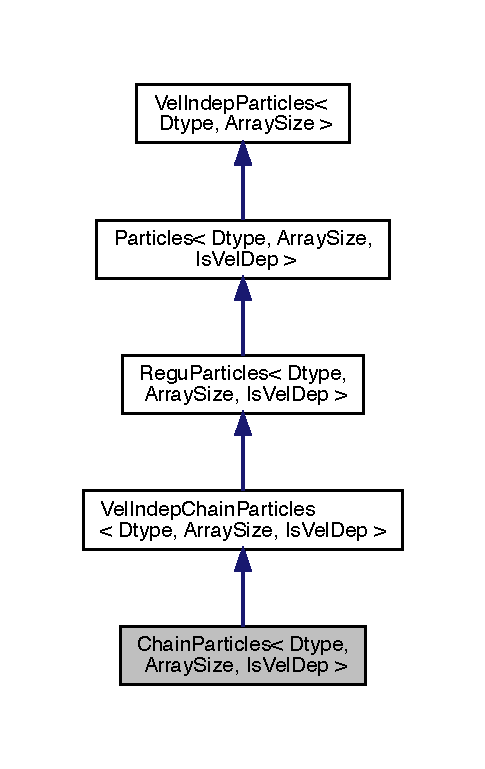
\includegraphics[width=233pt]{class_chain_particles__inherit__graph}
\end{center}
\end{figure}


Collaboration diagram for Chain\+Particles$<$ Dtype, Array\+Size, Is\+Vel\+Dep $>$\+:
\nopagebreak
\begin{figure}[H]
\begin{center}
\leavevmode
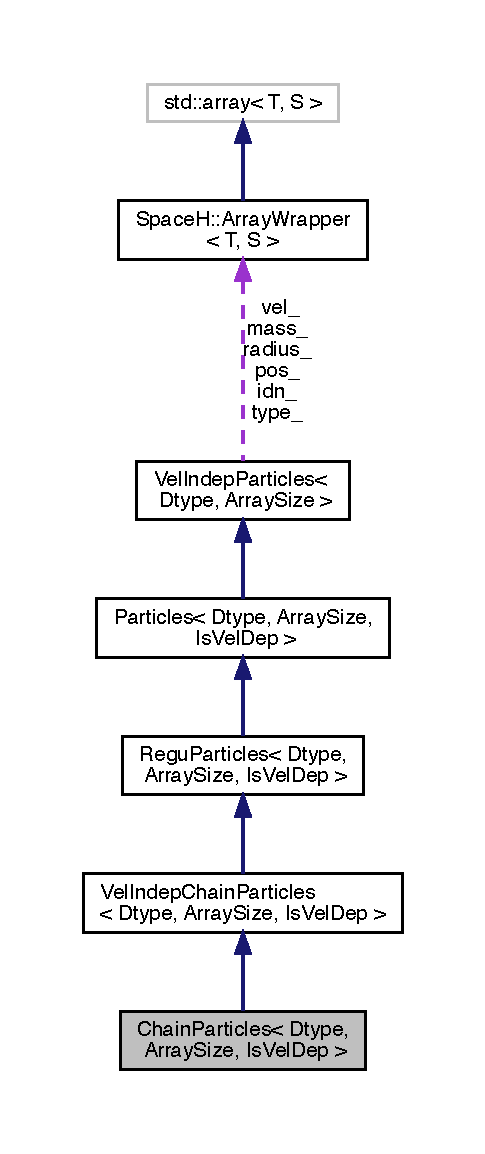
\includegraphics[height=550pt]{class_chain_particles__coll__graph}
\end{center}
\end{figure}
\subsection*{Additional Inherited Members}


\subsection{Detailed Description}
\subsubsection*{template$<$typename Dtype, size\+\_\+t Array\+Size, bool Is\+Vel\+Dep$>$\newline
class Chain\+Particles$<$ Dtype, Array\+Size, Is\+Vel\+Dep $>$}



Definition at line 256 of file dynamic\+Chain.\+h.



The documentation for this class was generated from the following file\+:\begin{DoxyCompactItemize}
\item 
particle\+System/\+A\+R\+Chain/\mbox{\hyperlink{dynamic_chain_8h}{dynamic\+Chain.\+h}}\end{DoxyCompactItemize}

\hypertarget{class_chain_particles_3_01_dtype_00_01_array_size_00_01true_01_4}{}\section{Chain\+Particles$<$ Dtype, Array\+Size, true $>$ Class Template Reference}
\label{class_chain_particles_3_01_dtype_00_01_array_size_00_01true_01_4}\index{Chain\+Particles$<$ Dtype, Array\+Size, true $>$@{Chain\+Particles$<$ Dtype, Array\+Size, true $>$}}


{\ttfamily \#include $<$dynamic\+Chain.\+h$>$}



Inheritance diagram for Chain\+Particles$<$ Dtype, Array\+Size, true $>$\+:
\nopagebreak
\begin{figure}[H]
\begin{center}
\leavevmode
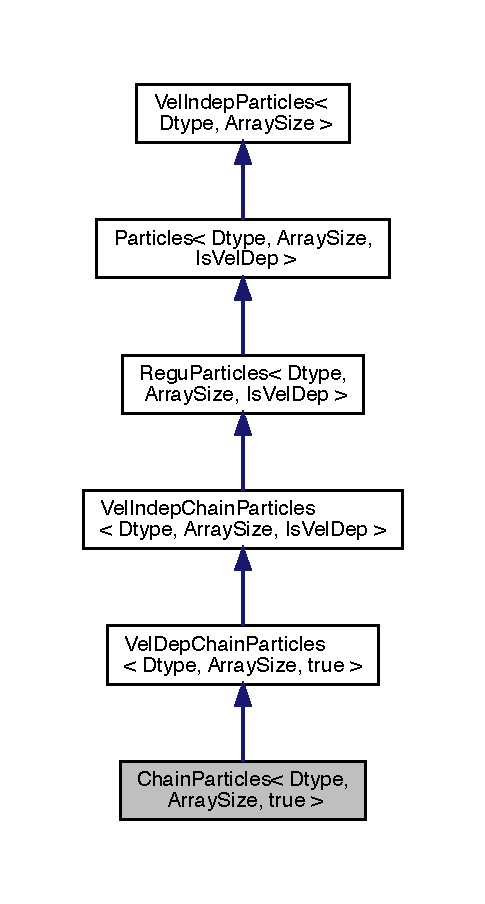
\includegraphics[width=233pt]{class_chain_particles_3_01_dtype_00_01_array_size_00_01true_01_4__inherit__graph}
\end{center}
\end{figure}


Collaboration diagram for Chain\+Particles$<$ Dtype, Array\+Size, true $>$\+:
\nopagebreak
\begin{figure}[H]
\begin{center}
\leavevmode
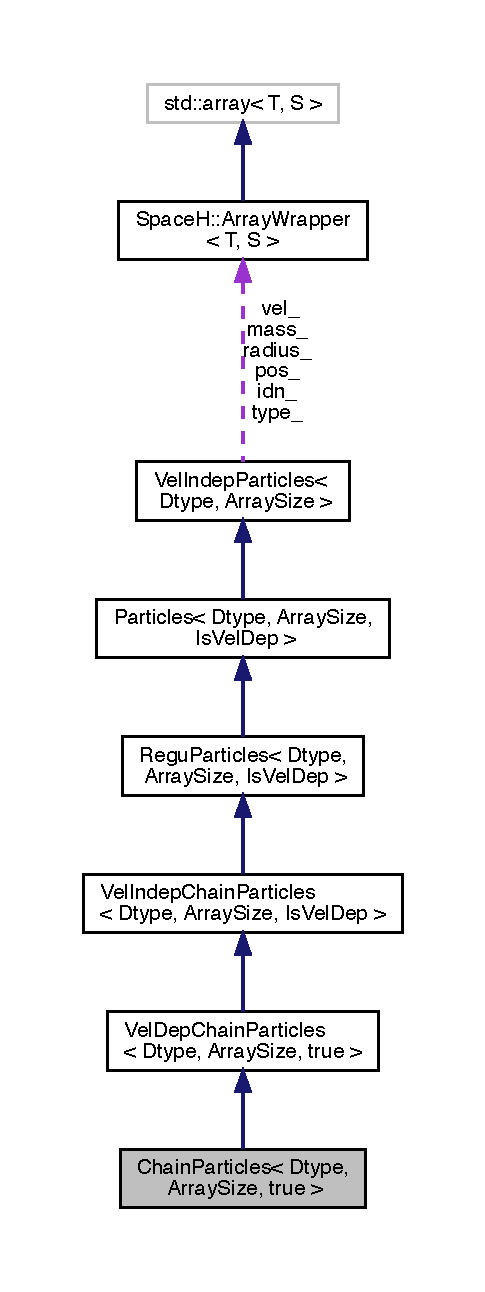
\includegraphics[height=550pt]{class_chain_particles_3_01_dtype_00_01_array_size_00_01true_01_4__coll__graph}
\end{center}
\end{figure}
\subsection*{Additional Inherited Members}


\subsection{Detailed Description}
\subsubsection*{template$<$typename Dtype, size\+\_\+t Array\+Size$>$\newline
class Chain\+Particles$<$ Dtype, Array\+Size, true $>$}



Definition at line 259 of file dynamic\+Chain.\+h.



The documentation for this class was generated from the following file\+:\begin{DoxyCompactItemize}
\item 
particle\+System/\+A\+R\+Chain/\mbox{\hyperlink{dynamic_chain_8h}{dynamic\+Chain.\+h}}\end{DoxyCompactItemize}

\hypertarget{classconst_iterator}{}\subsection{const\+Iterator$<$ Partic\+Sys, Integrator $>$ Class Template Reference}
\label{classconst_iterator}\index{const\+Iterator$<$ Partic\+Sys, Integrator $>$@{const\+Iterator$<$ Partic\+Sys, Integrator $>$}}


Most common iterator.  




{\ttfamily \#include $<$const\+Iterator.\+h$>$}

\subsubsection*{Public Types}
\begin{DoxyCompactItemize}
\item 
typedef Partic\+Sys\+::\+Scalar \mbox{\hyperlink{classconst_iterator_a7cdf84749facbb55a6a2674646f92f52}{Scalar}}
\begin{DoxyCompactList}\small\item\em interface to iterate particle system for one step \end{DoxyCompactList}\end{DoxyCompactItemize}
\subsubsection*{Public Member Functions}
\begin{DoxyCompactItemize}
\item 
\mbox{\hyperlink{classconst_iterator_a7cdf84749facbb55a6a2674646f92f52}{Scalar}} \mbox{\hyperlink{classconst_iterator_ac38af18a50fbb2aea54656f089911a48}{iterate}} (Partic\+Sys \&particles, Integrator \&integrator, \mbox{\hyperlink{classconst_iterator_a7cdf84749facbb55a6a2674646f92f52}{Scalar}} step\+Length)
\end{DoxyCompactItemize}


\subsubsection{Detailed Description}
\subsubsection*{template$<$typename Partic\+Sys, typename Integrator$>$\newline
class const\+Iterator$<$ Partic\+Sys, Integrator $>$}

Most common iterator. 

Constant iterator keep the step length constant and integrate the particle system for one step. 

\subsubsection{Member Typedef Documentation}
\mbox{\Hypertarget{classconst_iterator_a7cdf84749facbb55a6a2674646f92f52}\label{classconst_iterator_a7cdf84749facbb55a6a2674646f92f52}} 
\index{const\+Iterator@{const\+Iterator}!Scalar@{Scalar}}
\index{Scalar@{Scalar}!const\+Iterator@{const\+Iterator}}
\paragraph{\texorpdfstring{Scalar}{Scalar}}
{\footnotesize\ttfamily template$<$typename Partic\+Sys , typename Integrator $>$ \\
typedef Partic\+Sys\+::\+Scalar \mbox{\hyperlink{classconst_iterator}{const\+Iterator}}$<$ Partic\+Sys, Integrator $>$\+::\mbox{\hyperlink{classconst_iterator_a7cdf84749facbb55a6a2674646f92f52}{Scalar}}}



interface to iterate particle system for one step 


\begin{DoxyParams}{Parameters}
{\em particles} & Particle system needs evolution. \\
\hline
{\em integrator} & Integrator to integrate the particle system. \\
\hline
{\em step\+Length} & Macro step length for iteration(\+Here, the step length of the integrator). \\
\hline
\end{DoxyParams}
\begin{DoxyReturn}{Returns}
step length for next iteration. 
\end{DoxyReturn}


\subsubsection{Member Function Documentation}
\mbox{\Hypertarget{classconst_iterator_ac38af18a50fbb2aea54656f089911a48}\label{classconst_iterator_ac38af18a50fbb2aea54656f089911a48}} 
\index{const\+Iterator@{const\+Iterator}!iterate@{iterate}}
\index{iterate@{iterate}!const\+Iterator@{const\+Iterator}}
\paragraph{\texorpdfstring{iterate()}{iterate()}}
{\footnotesize\ttfamily template$<$typename Partic\+Sys , typename Integrator $>$ \\
\mbox{\hyperlink{classconst_iterator_a7cdf84749facbb55a6a2674646f92f52}{Scalar}} \mbox{\hyperlink{classconst_iterator}{const\+Iterator}}$<$ Partic\+Sys, Integrator $>$\+::iterate (\begin{DoxyParamCaption}\item[{Partic\+Sys \&}]{particles,  }\item[{Integrator \&}]{integrator,  }\item[{\mbox{\hyperlink{classconst_iterator_a7cdf84749facbb55a6a2674646f92f52}{Scalar}}}]{step\+Length }\end{DoxyParamCaption})\hspace{0.3cm}{\ttfamily [inline]}}



The documentation for this class was generated from the following file\+:\begin{DoxyCompactItemize}
\item 
O\+D\+Eiterator/\mbox{\hyperlink{const_iterator_8h}{const\+Iterator.\+h}}\end{DoxyCompactItemize}

\hypertarget{classdicho_iterator}{}\section{dicho\+Iterator$<$ Partic\+Sys, Integrator $>$ Class Template Reference}
\label{classdicho_iterator}\index{dicho\+Iterator$<$ Partic\+Sys, Integrator $>$@{dicho\+Iterator$<$ Partic\+Sys, Integrator $>$}}


Dichotomy iterator.  




{\ttfamily \#include $<$dichotomy.\+h$>$}

\subsection*{Public Types}
\begin{DoxyCompactItemize}
\item 
typedef Partic\+Sys\+::\+Scalar \mbox{\hyperlink{classdicho_iterator_a292e986136313822f21b1b60d9cbb95d}{Scalar}}
\item 
typedef Partic\+Sys\+::\+Plain\+Array \mbox{\hyperlink{classdicho_iterator_ab5b708b3b8a8fbd975c55231052d2547}{Plain\+Array}}
\end{DoxyCompactItemize}
\subsection*{Public Member Functions}
\begin{DoxyCompactItemize}
\item 
\mbox{\hyperlink{classdicho_iterator_a292e986136313822f21b1b60d9cbb95d}{Scalar}} \mbox{\hyperlink{classdicho_iterator_ad341b0652d8fb1530707893ed48a0257}{iterate}} (Partic\+Sys \&particles, \mbox{\hyperlink{classdicho_iterator_a292e986136313822f21b1b60d9cbb95d}{Scalar}} step\+Length)
\begin{DoxyCompactList}\small\item\em interface to iterate particle system for one step \end{DoxyCompactList}\item 
void \mbox{\hyperlink{classdicho_iterator_a2e810ce79342069faafde863d4876ce4}{set\+Relative\+Error}} (\mbox{\hyperlink{classdicho_iterator_a292e986136313822f21b1b60d9cbb95d}{Scalar}} rel\+Error)
\begin{DoxyCompactList}\small\item\em Set the local relative error. \end{DoxyCompactList}\item 
void \mbox{\hyperlink{classdicho_iterator_a95eaed5747897df265b2935a13eee8ca}{set\+Absolute\+Error}} (\mbox{\hyperlink{classdicho_iterator_a292e986136313822f21b1b60d9cbb95d}{Scalar}} abs\+Error)
\begin{DoxyCompactList}\small\item\em Set the local absolute error. \end{DoxyCompactList}\end{DoxyCompactItemize}


\subsection{Detailed Description}
\subsubsection*{template$<$typename Partic\+Sys, typename Integrator$>$\newline
class dicho\+Iterator$<$ Partic\+Sys, Integrator $>$}

Dichotomy iterator. 

Dichotomy iterator, use dichotomy to adjust the step size. 

\subsection{Member Typedef Documentation}
\mbox{\Hypertarget{classdicho_iterator_ab5b708b3b8a8fbd975c55231052d2547}\label{classdicho_iterator_ab5b708b3b8a8fbd975c55231052d2547}} 
\index{dicho\+Iterator@{dicho\+Iterator}!Plain\+Array@{Plain\+Array}}
\index{Plain\+Array@{Plain\+Array}!dicho\+Iterator@{dicho\+Iterator}}
\subsubsection{\texorpdfstring{Plain\+Array}{PlainArray}}
{\footnotesize\ttfamily template$<$typename Partic\+Sys , typename Integrator $>$ \\
typedef Partic\+Sys\+::\+Plain\+Array \mbox{\hyperlink{classdicho_iterator}{dicho\+Iterator}}$<$ Partic\+Sys, Integrator $>$\+::\mbox{\hyperlink{classdicho_iterator_ab5b708b3b8a8fbd975c55231052d2547}{Plain\+Array}}}

\mbox{\Hypertarget{classdicho_iterator_a292e986136313822f21b1b60d9cbb95d}\label{classdicho_iterator_a292e986136313822f21b1b60d9cbb95d}} 
\index{dicho\+Iterator@{dicho\+Iterator}!Scalar@{Scalar}}
\index{Scalar@{Scalar}!dicho\+Iterator@{dicho\+Iterator}}
\subsubsection{\texorpdfstring{Scalar}{Scalar}}
{\footnotesize\ttfamily template$<$typename Partic\+Sys , typename Integrator $>$ \\
typedef Partic\+Sys\+::\+Scalar \mbox{\hyperlink{classdicho_iterator}{dicho\+Iterator}}$<$ Partic\+Sys, Integrator $>$\+::\mbox{\hyperlink{classdicho_iterator_a292e986136313822f21b1b60d9cbb95d}{Scalar}}}



\subsection{Member Function Documentation}
\mbox{\Hypertarget{classdicho_iterator_ad341b0652d8fb1530707893ed48a0257}\label{classdicho_iterator_ad341b0652d8fb1530707893ed48a0257}} 
\index{dicho\+Iterator@{dicho\+Iterator}!iterate@{iterate}}
\index{iterate@{iterate}!dicho\+Iterator@{dicho\+Iterator}}
\subsubsection{\texorpdfstring{iterate()}{iterate()}}
{\footnotesize\ttfamily template$<$typename Partic\+Sys , typename Integrator $>$ \\
\mbox{\hyperlink{test_orbit_8cpp_a8c2981f3f834be9448a6ab06c28748eb}{Partic\+Sys\+::\+Scalar}} \mbox{\hyperlink{classdicho_iterator}{dicho\+Iterator}}$<$ Partic\+Sys, Integrator $>$\+::iterate (\begin{DoxyParamCaption}\item[{Partic\+Sys \&}]{particles,  }\item[{\mbox{\hyperlink{classdicho_iterator_a292e986136313822f21b1b60d9cbb95d}{Scalar}}}]{step\+Length }\end{DoxyParamCaption})}



interface to iterate particle system for one step 


\begin{DoxyParams}{Parameters}
{\em particles} & Particle system needs evolution. \\
\hline
{\em integrator} & Integrator to integrate the particle system. \\
\hline
{\em step\+Length} & Macro step length for iteration(\+Here, the step length of the integrator). \\
\hline
\end{DoxyParams}
\begin{DoxyReturn}{Returns}
step length for next iteration. 
\end{DoxyReturn}
\mbox{\Hypertarget{classdicho_iterator_a95eaed5747897df265b2935a13eee8ca}\label{classdicho_iterator_a95eaed5747897df265b2935a13eee8ca}} 
\index{dicho\+Iterator@{dicho\+Iterator}!set\+Absolute\+Error@{set\+Absolute\+Error}}
\index{set\+Absolute\+Error@{set\+Absolute\+Error}!dicho\+Iterator@{dicho\+Iterator}}
\subsubsection{\texorpdfstring{set\+Absolute\+Error()}{setAbsoluteError()}}
{\footnotesize\ttfamily template$<$typename Partic\+Sys , typename Integrator $>$ \\
void \mbox{\hyperlink{classdicho_iterator}{dicho\+Iterator}}$<$ Partic\+Sys, Integrator $>$\+::set\+Absolute\+Error (\begin{DoxyParamCaption}\item[{\mbox{\hyperlink{classdicho_iterator_a292e986136313822f21b1b60d9cbb95d}{Scalar}}}]{abs\+Error }\end{DoxyParamCaption})\hspace{0.3cm}{\ttfamily [inline]}}



Set the local absolute error. 

\mbox{\Hypertarget{classdicho_iterator_a2e810ce79342069faafde863d4876ce4}\label{classdicho_iterator_a2e810ce79342069faafde863d4876ce4}} 
\index{dicho\+Iterator@{dicho\+Iterator}!set\+Relative\+Error@{set\+Relative\+Error}}
\index{set\+Relative\+Error@{set\+Relative\+Error}!dicho\+Iterator@{dicho\+Iterator}}
\subsubsection{\texorpdfstring{set\+Relative\+Error()}{setRelativeError()}}
{\footnotesize\ttfamily template$<$typename Partic\+Sys , typename Integrator $>$ \\
void \mbox{\hyperlink{classdicho_iterator}{dicho\+Iterator}}$<$ Partic\+Sys, Integrator $>$\+::set\+Relative\+Error (\begin{DoxyParamCaption}\item[{\mbox{\hyperlink{classdicho_iterator_a292e986136313822f21b1b60d9cbb95d}{Scalar}}}]{rel\+Error }\end{DoxyParamCaption})\hspace{0.3cm}{\ttfamily [inline]}}



Set the local relative error. 



The documentation for this class was generated from the following file\+:\begin{DoxyCompactItemize}
\item 
O\+D\+Eiterator/\mbox{\hyperlink{dichotomy_8h}{dichotomy.\+h}}\end{DoxyCompactItemize}

\hypertarget{structdtype}{}\section{dtype$<$ T $>$ Struct Template Reference}
\label{structdtype}\index{dtype$<$ T $>$@{dtype$<$ T $>$}}
\subsection*{Public Types}
\begin{DoxyCompactItemize}
\item 
using \mbox{\hyperlink{structdtype_a2c7a9959a8b61a98cc065f03eaa79e89}{type}} = decltype(\mbox{\hyperlink{structdtype_a70fa7f25bb22166e7788e045e62f6a64}{check}}$<$ T $>$(0))
\end{DoxyCompactItemize}
\subsection*{Static Public Member Functions}
\begin{DoxyCompactItemize}
\item 
{\footnotesize template$<$typename U $>$ }\\static U\+::value\+\_\+type \mbox{\hyperlink{structdtype_a70fa7f25bb22166e7788e045e62f6a64}{check}} (typename U\+::value\+\_\+type)
\item 
{\footnotesize template$<$typename U $>$ }\\static U \mbox{\hyperlink{structdtype_a01282018f55ad532f28b1605af093999}{check}} (U)
\end{DoxyCompactItemize}


\subsection{Detailed Description}
\subsubsection*{template$<$typename T$>$\newline
struct dtype$<$ T $>$}



Definition at line 9 of file typetest.\+cpp.



\subsection{Member Typedef Documentation}
\mbox{\Hypertarget{structdtype_a2c7a9959a8b61a98cc065f03eaa79e89}\label{structdtype_a2c7a9959a8b61a98cc065f03eaa79e89}} 
\index{dtype@{dtype}!type@{type}}
\index{type@{type}!dtype@{dtype}}
\subsubsection{\texorpdfstring{type}{type}}
{\footnotesize\ttfamily template$<$typename T $>$ \\
using \mbox{\hyperlink{structdtype}{dtype}}$<$ T $>$\+::\mbox{\hyperlink{structdtype_a2c7a9959a8b61a98cc065f03eaa79e89}{type}} =  decltype(\mbox{\hyperlink{structdtype_a70fa7f25bb22166e7788e045e62f6a64}{check}}$<$T$>$(0))}



Definition at line 17 of file typetest.\+cpp.



\subsection{Member Function Documentation}
\mbox{\Hypertarget{structdtype_a70fa7f25bb22166e7788e045e62f6a64}\label{structdtype_a70fa7f25bb22166e7788e045e62f6a64}} 
\index{dtype@{dtype}!check@{check}}
\index{check@{check}!dtype@{dtype}}
\subsubsection{\texorpdfstring{check()}{check()}\hspace{0.1cm}{\footnotesize\ttfamily [1/2]}}
{\footnotesize\ttfamily template$<$typename T $>$ \\
template$<$typename U $>$ \\
static U\+::value\+\_\+type \mbox{\hyperlink{structdtype}{dtype}}$<$ T $>$\+::check (\begin{DoxyParamCaption}\item[{typename U\+::value\+\_\+type}]{ }\end{DoxyParamCaption})\hspace{0.3cm}{\ttfamily [static]}}

\mbox{\Hypertarget{structdtype_a01282018f55ad532f28b1605af093999}\label{structdtype_a01282018f55ad532f28b1605af093999}} 
\index{dtype@{dtype}!check@{check}}
\index{check@{check}!dtype@{dtype}}
\subsubsection{\texorpdfstring{check()}{check()}\hspace{0.1cm}{\footnotesize\ttfamily [2/2]}}
{\footnotesize\ttfamily template$<$typename T $>$ \\
template$<$typename U $>$ \\
static U \mbox{\hyperlink{structdtype}{dtype}}$<$ T $>$\+::check (\begin{DoxyParamCaption}\item[{U}]{ }\end{DoxyParamCaption})\hspace{0.3cm}{\ttfamily [static]}}



The documentation for this struct was generated from the following file\+:\begin{DoxyCompactItemize}
\item 
test/\mbox{\hyperlink{typetest_8cpp}{typetest.\+cpp}}\end{DoxyCompactItemize}

\hypertarget{classdynamic_system}{}\section{dynamic\+System$<$ Partic\+Sys, O\+D\+Eiterator $>$ Class Template Reference}
\label{classdynamic_system}\index{dynamic\+System$<$ Partic\+Sys, O\+D\+Eiterator $>$@{dynamic\+System$<$ Partic\+Sys, O\+D\+Eiterator $>$}}


A wrapper to make particle system, integrator and O\+DE iterator work together.  




{\ttfamily \#include $<$dynamic\+System.\+h$>$}

\subsection*{Public Types}
\begin{DoxyCompactItemize}
\item 
using \mbox{\hyperlink{classdynamic_system_a518990ebef8f3f6257e6ef0e49fe013e}{type}} = typename Partic\+Sys\+::type
\item 
using \mbox{\hyperlink{classdynamic_system_a6eb7b06a4ee5721a1ee0855a854c3431}{Scalar}} = typename type\+::\+Scalar
\end{DoxyCompactItemize}
\subsection*{Public Member Functions}
\begin{DoxyCompactItemize}
\item 
void \mbox{\hyperlink{classdynamic_system_a7a4032c043dd0286007f4d7c542d3f95}{advance\+One\+Step}} ()
\begin{DoxyCompactList}\small\item\em Advance the particle system for one step. \end{DoxyCompactList}\item 
void \mbox{\hyperlink{classdynamic_system_a3ff4342241733e94edce17c1a79a90a8}{load\+Text}} (char const $\ast$init\+File\+Path)
\begin{DoxyCompactList}\small\item\em Load particle system initial condition from file. \end{DoxyCompactList}\item 
void \mbox{\hyperlink{classdynamic_system_a0392d5b36a03692d65616f3b40168948}{set\+Step\+Length}} (\mbox{\hyperlink{classdynamic_system_a6eb7b06a4ee5721a1ee0855a854c3431}{Scalar}})
\begin{DoxyCompactList}\small\item\em Set the step length. \end{DoxyCompactList}\item 
virtual \mbox{\hyperlink{classdynamic_system_a239af38fcf35f3fe32d5ae5e183e4cca}{$\sim$dynamic\+System}} ()
\begin{DoxyCompactList}\small\item\em Default destructor, virtualize for inherent class. \end{DoxyCompactList}\end{DoxyCompactItemize}
\subsection*{Public Attributes}
\begin{DoxyCompactItemize}
\item 
\mbox{\hyperlink{classdynamic_system_a6eb7b06a4ee5721a1ee0855a854c3431}{Scalar}} \mbox{\hyperlink{classdynamic_system_a3f0e5b7ef17b728c723c67aefa9dbada}{step\+Length}} \{0.\+0\}
\begin{DoxyCompactList}\small\item\em Macro step size for O\+DE iterator. \end{DoxyCompactList}\item 
int \mbox{\hyperlink{classdynamic_system_ae9821e179896e6cddbbcc4e706552c57}{steps}} \{0\}
\begin{DoxyCompactList}\small\item\em Steps. \end{DoxyCompactList}\item 
Partic\+Sys \mbox{\hyperlink{classdynamic_system_a809657c0ef63741a7e3d6f32bc87bfe3}{particles}}
\begin{DoxyCompactList}\small\item\em Particle system. \end{DoxyCompactList}\item 
O\+D\+Eiterator \mbox{\hyperlink{classdynamic_system_a0a13a11664ce5761ab4296b1b0421f99}{iterator}}
\begin{DoxyCompactList}\small\item\em O\+DE Iterator. \end{DoxyCompactList}\end{DoxyCompactItemize}


\subsection{Detailed Description}
\subsubsection*{template$<$typename Partic\+Sys, typename O\+D\+Eiterator$>$\newline
class dynamic\+System$<$ Partic\+Sys, O\+D\+Eiterator $>$}

A wrapper to make particle system, integrator and O\+DE iterator work together. 

Definition at line 31 of file dynamic\+System.\+h.



\subsection{Member Typedef Documentation}
\mbox{\Hypertarget{classdynamic_system_a6eb7b06a4ee5721a1ee0855a854c3431}\label{classdynamic_system_a6eb7b06a4ee5721a1ee0855a854c3431}} 
\index{dynamic\+System@{dynamic\+System}!Scalar@{Scalar}}
\index{Scalar@{Scalar}!dynamic\+System@{dynamic\+System}}
\subsubsection{\texorpdfstring{Scalar}{Scalar}}
{\footnotesize\ttfamily template$<$typename Partic\+Sys , typename O\+D\+Eiterator $>$ \\
using \mbox{\hyperlink{classdynamic_system}{dynamic\+System}}$<$ Partic\+Sys, O\+D\+Eiterator $>$\+::\mbox{\hyperlink{classdynamic_system_a6eb7b06a4ee5721a1ee0855a854c3431}{Scalar}} =  typename type\+::\+Scalar}



Definition at line 35 of file dynamic\+System.\+h.

\mbox{\Hypertarget{classdynamic_system_a518990ebef8f3f6257e6ef0e49fe013e}\label{classdynamic_system_a518990ebef8f3f6257e6ef0e49fe013e}} 
\index{dynamic\+System@{dynamic\+System}!type@{type}}
\index{type@{type}!dynamic\+System@{dynamic\+System}}
\subsubsection{\texorpdfstring{type}{type}}
{\footnotesize\ttfamily template$<$typename Partic\+Sys , typename O\+D\+Eiterator $>$ \\
using \mbox{\hyperlink{classdynamic_system}{dynamic\+System}}$<$ Partic\+Sys, O\+D\+Eiterator $>$\+::\mbox{\hyperlink{classdynamic_system_a518990ebef8f3f6257e6ef0e49fe013e}{type}} =  typename Partic\+Sys\+::type}



Definition at line 34 of file dynamic\+System.\+h.



\subsection{Constructor \& Destructor Documentation}
\mbox{\Hypertarget{classdynamic_system_a239af38fcf35f3fe32d5ae5e183e4cca}\label{classdynamic_system_a239af38fcf35f3fe32d5ae5e183e4cca}} 
\index{dynamic\+System@{dynamic\+System}!````~dynamic\+System@{$\sim$dynamic\+System}}
\index{````~dynamic\+System@{$\sim$dynamic\+System}!dynamic\+System@{dynamic\+System}}
\subsubsection{\texorpdfstring{$\sim$dynamic\+System()}{~dynamicSystem()}}
{\footnotesize\ttfamily template$<$typename Partic\+Sys , typename O\+D\+Eiterator $>$ \\
virtual \mbox{\hyperlink{classdynamic_system}{dynamic\+System}}$<$ Partic\+Sys, O\+D\+Eiterator $>$\+::$\sim$\mbox{\hyperlink{classdynamic_system}{dynamic\+System}} (\begin{DoxyParamCaption}{ }\end{DoxyParamCaption})\hspace{0.3cm}{\ttfamily [inline]}, {\ttfamily [virtual]}}



Default destructor, virtualize for inherent class. 



Definition at line 40 of file dynamic\+System.\+h.



\subsection{Member Function Documentation}
\mbox{\Hypertarget{classdynamic_system_a7a4032c043dd0286007f4d7c542d3f95}\label{classdynamic_system_a7a4032c043dd0286007f4d7c542d3f95}} 
\index{dynamic\+System@{dynamic\+System}!advance\+One\+Step@{advance\+One\+Step}}
\index{advance\+One\+Step@{advance\+One\+Step}!dynamic\+System@{dynamic\+System}}
\subsubsection{\texorpdfstring{advance\+One\+Step()}{advanceOneStep()}}
{\footnotesize\ttfamily template$<$typename Partic\+Sys , typename O\+D\+Eiterator $>$ \\
void \mbox{\hyperlink{classdynamic_system}{dynamic\+System}}$<$ Partic\+Sys, O\+D\+Eiterator $>$\+::advance\+One\+Step (\begin{DoxyParamCaption}{ }\end{DoxyParamCaption})\hspace{0.3cm}{\ttfamily [inline]}}



Advance the particle system for one step. 

Advance the particle system with current steplength step\+Length. The O\+DE iterator iterate the integrator to convergence by its own implement. The step length will also be updated by its own implement. 

Definition at line 65 of file dynamic\+System.\+h.

\mbox{\Hypertarget{classdynamic_system_a3ff4342241733e94edce17c1a79a90a8}\label{classdynamic_system_a3ff4342241733e94edce17c1a79a90a8}} 
\index{dynamic\+System@{dynamic\+System}!load\+Text@{load\+Text}}
\index{load\+Text@{load\+Text}!dynamic\+System@{dynamic\+System}}
\subsubsection{\texorpdfstring{load\+Text()}{loadText()}}
{\footnotesize\ttfamily template$<$typename Partic\+Sys , typename O\+D\+Eiterator $>$ \\
void \mbox{\hyperlink{classdynamic_system}{dynamic\+System}}$<$ Partic\+Sys, O\+D\+Eiterator $>$\+::load\+Text (\begin{DoxyParamCaption}\item[{char const $\ast$}]{init\+File\+Path }\end{DoxyParamCaption})}



Load particle system initial condition from file. 

This function will read and check the initial file header (begin with \textquotesingle{}\#\textquotesingle{}) and the particle number after the \textquotesingle{}\#\textquotesingle{}. Pass the rest information to particles by operator \textquotesingle{}$>$$>$\textquotesingle{}. The way to load the initial condition depend on the implemet of the particles. If the initial condition read successfully. This function will call get\+Init\+Step\+Length() to set the initial step length.


\begin{DoxyParams}{Parameters}
{\em init\+File\+Path} & The relative path of initial conditions file \\
\hline
\end{DoxyParams}

\begin{DoxyExceptions}{Exceptions}
{\em If} & the partcile number in the header is inconsisitent with the size of particles, this function will throw an exception. \\
\hline
\end{DoxyExceptions}


Definition at line 103 of file dynamic\+System.\+h.

Here is the caller graph for this function\+:\nopagebreak
\begin{figure}[H]
\begin{center}
\leavevmode
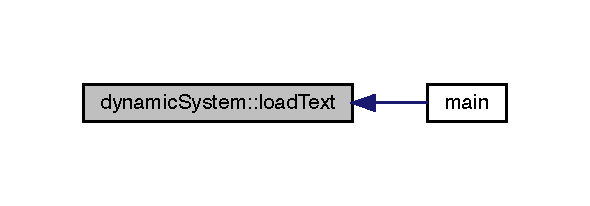
\includegraphics[width=283pt]{classdynamic_system_a3ff4342241733e94edce17c1a79a90a8_icgraph}
\end{center}
\end{figure}
\mbox{\Hypertarget{classdynamic_system_a0392d5b36a03692d65616f3b40168948}\label{classdynamic_system_a0392d5b36a03692d65616f3b40168948}} 
\index{dynamic\+System@{dynamic\+System}!set\+Step\+Length@{set\+Step\+Length}}
\index{set\+Step\+Length@{set\+Step\+Length}!dynamic\+System@{dynamic\+System}}
\subsubsection{\texorpdfstring{set\+Step\+Length()}{setStepLength()}}
{\footnotesize\ttfamily template$<$typename Partic\+Sys , typename O\+D\+Eiterator $>$ \\
void \mbox{\hyperlink{classdynamic_system}{dynamic\+System}}$<$ Partic\+Sys, O\+D\+Eiterator $>$\+::set\+Step\+Length (\begin{DoxyParamCaption}\item[{\mbox{\hyperlink{classdynamic_system_a6eb7b06a4ee5721a1ee0855a854c3431}{Scalar}}}]{step\+Size }\end{DoxyParamCaption})}



Set the step length. 



Definition at line 132 of file dynamic\+System.\+h.



\subsection{Member Data Documentation}
\mbox{\Hypertarget{classdynamic_system_a0a13a11664ce5761ab4296b1b0421f99}\label{classdynamic_system_a0a13a11664ce5761ab4296b1b0421f99}} 
\index{dynamic\+System@{dynamic\+System}!iterator@{iterator}}
\index{iterator@{iterator}!dynamic\+System@{dynamic\+System}}
\subsubsection{\texorpdfstring{iterator}{iterator}}
{\footnotesize\ttfamily template$<$typename Partic\+Sys , typename O\+D\+Eiterator $>$ \\
O\+D\+Eiterator \mbox{\hyperlink{classdynamic_system}{dynamic\+System}}$<$ Partic\+Sys, O\+D\+Eiterator $>$\+::iterator}



O\+DE Iterator. 



Definition at line 52 of file dynamic\+System.\+h.

\mbox{\Hypertarget{classdynamic_system_a809657c0ef63741a7e3d6f32bc87bfe3}\label{classdynamic_system_a809657c0ef63741a7e3d6f32bc87bfe3}} 
\index{dynamic\+System@{dynamic\+System}!particles@{particles}}
\index{particles@{particles}!dynamic\+System@{dynamic\+System}}
\subsubsection{\texorpdfstring{particles}{particles}}
{\footnotesize\ttfamily template$<$typename Partic\+Sys , typename O\+D\+Eiterator $>$ \\
Partic\+Sys \mbox{\hyperlink{classdynamic_system}{dynamic\+System}}$<$ Partic\+Sys, O\+D\+Eiterator $>$\+::particles}



Particle system. 



Definition at line 49 of file dynamic\+System.\+h.

\mbox{\Hypertarget{classdynamic_system_a3f0e5b7ef17b728c723c67aefa9dbada}\label{classdynamic_system_a3f0e5b7ef17b728c723c67aefa9dbada}} 
\index{dynamic\+System@{dynamic\+System}!step\+Length@{step\+Length}}
\index{step\+Length@{step\+Length}!dynamic\+System@{dynamic\+System}}
\subsubsection{\texorpdfstring{step\+Length}{stepLength}}
{\footnotesize\ttfamily template$<$typename Partic\+Sys , typename O\+D\+Eiterator $>$ \\
\mbox{\hyperlink{classdynamic_system_a6eb7b06a4ee5721a1ee0855a854c3431}{Scalar}} \mbox{\hyperlink{classdynamic_system}{dynamic\+System}}$<$ Partic\+Sys, O\+D\+Eiterator $>$\+::step\+Length \{0.\+0\}}



Macro step size for O\+DE iterator. 



Definition at line 43 of file dynamic\+System.\+h.

\mbox{\Hypertarget{classdynamic_system_ae9821e179896e6cddbbcc4e706552c57}\label{classdynamic_system_ae9821e179896e6cddbbcc4e706552c57}} 
\index{dynamic\+System@{dynamic\+System}!steps@{steps}}
\index{steps@{steps}!dynamic\+System@{dynamic\+System}}
\subsubsection{\texorpdfstring{steps}{steps}}
{\footnotesize\ttfamily template$<$typename Partic\+Sys , typename O\+D\+Eiterator $>$ \\
int \mbox{\hyperlink{classdynamic_system}{dynamic\+System}}$<$ Partic\+Sys, O\+D\+Eiterator $>$\+::steps \{0\}}



Steps. 



Definition at line 46 of file dynamic\+System.\+h.



The documentation for this class was generated from the following file\+:\begin{DoxyCompactItemize}
\item 
\mbox{\hyperlink{dynamic_system_8h}{dynamic\+System.\+h}}\end{DoxyCompactItemize}

\hypertarget{struct_space_h_1_1_empty_class}{}\section{SpaceH\+:\+:Empty\+Class Struct Reference}
\label{struct_space_h_1_1_empty_class}\index{Space\+H\+::\+Empty\+Class@{Space\+H\+::\+Empty\+Class}}


{\ttfamily \#include $<$proto\+Type.\+h$>$}



The documentation for this struct was generated from the following file\+:\begin{DoxyCompactItemize}
\item 
\mbox{\hyperlink{proto_type_8h}{proto\+Type.\+h}}\end{DoxyCompactItemize}

\hypertarget{struct_space_h_1_1_empty_force}{}\section{SpaceH\+:\+:Empty\+Force$<$ Dtype, Array\+Size $>$ Struct Template Reference}
\label{struct_space_h_1_1_empty_force}\index{Space\+H\+::\+Empty\+Force$<$ Dtype, Array\+Size $>$@{Space\+H\+::\+Empty\+Force$<$ Dtype, Array\+Size $>$}}


{\ttfamily \#include $<$forces.\+h$>$}

\subsection*{Public Types}
\begin{DoxyCompactItemize}
\item 
using \mbox{\hyperlink{struct_space_h_1_1_empty_force_a87b62085a73d95239597b9e88ff5e32a}{type}} = \mbox{\hyperlink{struct_space_h_1_1_proto_type}{Space\+H\+::\+Proto\+Type}}$<$ Dtype, Array\+Size $>$
\item 
using \mbox{\hyperlink{struct_space_h_1_1_empty_force_a708ead350efe0aa6f7bf1c0909ee6f28}{Scalar}} = typename \mbox{\hyperlink{struct_space_h_1_1_proto_type_af3c8245d83d9db64749882920de5c274}{type\+::\+Scalar}}
\item 
using \mbox{\hyperlink{struct_space_h_1_1_empty_force_abfd8a2b724383a3a2dde191d95ca0661}{Vector}} = typename \mbox{\hyperlink{struct_space_h_1_1_proto_type_a316b81f4660b2b4fab14a8e1f23b6089}{type\+::\+Vector}}
\item 
using \mbox{\hyperlink{struct_space_h_1_1_empty_force_a06ad868879a6fa5def9c7f9fd75fffde}{Vector\+Array}} = typename \mbox{\hyperlink{struct_space_h_1_1_proto_type_a622b8e122b33bb4966a02299fb7b82d6}{type\+::\+Vector\+Array}}
\item 
using \mbox{\hyperlink{struct_space_h_1_1_empty_force_afdeb66410650cdb1e2e3b1e1fd79540c}{Scalar\+Array}} = typename \mbox{\hyperlink{struct_space_h_1_1_proto_type_a09ef91dc8a37a044c403f5a833044725}{type\+::\+Scalar\+Array}}
\item 
using \mbox{\hyperlink{struct_space_h_1_1_empty_force_a25e0bd933dd3715e315c1abdb6843c36}{Index\+Array}} = typename \mbox{\hyperlink{struct_space_h_1_1_proto_type_a276a37c81faf08681b57e8082f3f6c1b}{type\+::\+Index\+Array}}
\end{DoxyCompactItemize}
\subsection*{Public Member Functions}
\begin{DoxyCompactItemize}
\item 
void \mbox{\hyperlink{struct_space_h_1_1_empty_force_a83468f94ac05624de3f8e492f3171560}{calcu\+Acc}} (const \mbox{\hyperlink{struct_space_h_1_1_empty_force_afdeb66410650cdb1e2e3b1e1fd79540c}{Scalar\+Array}} \&mass, const \mbox{\hyperlink{struct_space_h_1_1_empty_force_a06ad868879a6fa5def9c7f9fd75fffde}{Vector\+Array}} \&pos)
\item 
void \mbox{\hyperlink{struct_space_h_1_1_empty_force_af5373ca3798b19d9b4eb155c3fe7cf46}{calcu\+Acc}} (const \mbox{\hyperlink{struct_space_h_1_1_empty_force_afdeb66410650cdb1e2e3b1e1fd79540c}{Scalar\+Array}} \&mass, const \mbox{\hyperlink{struct_space_h_1_1_empty_force_a06ad868879a6fa5def9c7f9fd75fffde}{Vector\+Array}} \&pos, const \mbox{\hyperlink{struct_space_h_1_1_empty_force_a06ad868879a6fa5def9c7f9fd75fffde}{Vector\+Array}} \&vel)
\item 
void \mbox{\hyperlink{struct_space_h_1_1_empty_force_aef0a45bc07150151ac18c6e180784e56}{calcu\+Acc}} (const \mbox{\hyperlink{struct_space_h_1_1_empty_force_afdeb66410650cdb1e2e3b1e1fd79540c}{Scalar\+Array}} \&mass, const \mbox{\hyperlink{struct_space_h_1_1_empty_force_a06ad868879a6fa5def9c7f9fd75fffde}{Vector\+Array}} \&pos, const \mbox{\hyperlink{struct_space_h_1_1_empty_force_a06ad868879a6fa5def9c7f9fd75fffde}{Vector\+Array}} \&chain_\+Pos, const \mbox{\hyperlink{struct_space_h_1_1_empty_force_a25e0bd933dd3715e315c1abdb6843c36}{Index\+Array}} \&chain_\+Index)
\item 
void \mbox{\hyperlink{struct_space_h_1_1_empty_force_a60c8642978737f561503d41d3dee90d7}{calcu\+Acc}} (const \mbox{\hyperlink{struct_space_h_1_1_empty_force_afdeb66410650cdb1e2e3b1e1fd79540c}{Scalar\+Array}} \&mass, const \mbox{\hyperlink{struct_space_h_1_1_empty_force_a06ad868879a6fa5def9c7f9fd75fffde}{Vector\+Array}} \&pos, const \mbox{\hyperlink{struct_space_h_1_1_empty_force_a06ad868879a6fa5def9c7f9fd75fffde}{Vector\+Array}} \&vel, const \mbox{\hyperlink{struct_space_h_1_1_empty_force_a06ad868879a6fa5def9c7f9fd75fffde}{Vector\+Array}} \&chain_\+Pos, const \mbox{\hyperlink{struct_space_h_1_1_empty_force_a06ad868879a6fa5def9c7f9fd75fffde}{Vector\+Array}} \&chain_\+Vel, const \mbox{\hyperlink{struct_space_h_1_1_empty_force_a25e0bd933dd3715e315c1abdb6843c36}{Index\+Array}} \&chain_\+Index)
\item 
void \mbox{\hyperlink{struct_space_h_1_1_empty_force_a6aed735e5443a08ad6e70ae6bcd74bf8}{add\+Total}} (\mbox{\hyperlink{struct_space_h_1_1_empty_force_a06ad868879a6fa5def9c7f9fd75fffde}{Vector\+Array}} \&\mbox{\hyperlink{struct_space_h_1_1_empty_force_a1547f680e4dbf0cb9fc7e945872928e2}{acc}})
\item 
const \mbox{\hyperlink{struct_space_h_1_1_empty_force_a06ad868879a6fa5def9c7f9fd75fffde}{Vector\+Array}} \& \mbox{\hyperlink{struct_space_h_1_1_empty_force_a1547f680e4dbf0cb9fc7e945872928e2}{acc}} ()
\item 
const \mbox{\hyperlink{struct_space_h_1_1_empty_force_abfd8a2b724383a3a2dde191d95ca0661}{Vector}} \& \mbox{\hyperlink{struct_space_h_1_1_empty_force_aef51b27e9c50c23783619e82dca0b1e6}{acc}} (size\+\_\+t i)
\end{DoxyCompactItemize}
\subsection*{Static Public Attributes}
\begin{DoxyCompactItemize}
\item 
static constexpr bool \mbox{\hyperlink{struct_space_h_1_1_empty_force_a9c02c91b7ec657b88c89ef02307ca4b5}{is\+Vel\+Dep}} \{false\}
\end{DoxyCompactItemize}


\subsection{Detailed Description}
\subsubsection*{template$<$typename Dtype, size\+\_\+t Array\+Size$>$\newline
struct Space\+H\+::\+Empty\+Force$<$ Dtype, Array\+Size $>$}



Definition at line 22 of file forces.\+h.



\subsection{Member Typedef Documentation}
\mbox{\Hypertarget{struct_space_h_1_1_empty_force_a25e0bd933dd3715e315c1abdb6843c36}\label{struct_space_h_1_1_empty_force_a25e0bd933dd3715e315c1abdb6843c36}} 
\index{Space\+H\+::\+Empty\+Force@{Space\+H\+::\+Empty\+Force}!Index\+Array@{Index\+Array}}
\index{Index\+Array@{Index\+Array}!Space\+H\+::\+Empty\+Force@{Space\+H\+::\+Empty\+Force}}
\subsubsection{\texorpdfstring{Index\+Array}{IndexArray}}
{\footnotesize\ttfamily template$<$typename Dtype , size\+\_\+t Array\+Size$>$ \\
using \mbox{\hyperlink{struct_space_h_1_1_empty_force}{Space\+H\+::\+Empty\+Force}}$<$ Dtype, Array\+Size $>$\+::\mbox{\hyperlink{struct_space_h_1_1_empty_force_a25e0bd933dd3715e315c1abdb6843c36}{Index\+Array}} =  typename \mbox{\hyperlink{struct_space_h_1_1_proto_type_a276a37c81faf08681b57e8082f3f6c1b}{type\+::\+Index\+Array}}}



Definition at line 35 of file forces.\+h.

\mbox{\Hypertarget{struct_space_h_1_1_empty_force_a708ead350efe0aa6f7bf1c0909ee6f28}\label{struct_space_h_1_1_empty_force_a708ead350efe0aa6f7bf1c0909ee6f28}} 
\index{Space\+H\+::\+Empty\+Force@{Space\+H\+::\+Empty\+Force}!Scalar@{Scalar}}
\index{Scalar@{Scalar}!Space\+H\+::\+Empty\+Force@{Space\+H\+::\+Empty\+Force}}
\subsubsection{\texorpdfstring{Scalar}{Scalar}}
{\footnotesize\ttfamily template$<$typename Dtype , size\+\_\+t Array\+Size$>$ \\
using \mbox{\hyperlink{struct_space_h_1_1_empty_force}{Space\+H\+::\+Empty\+Force}}$<$ Dtype, Array\+Size $>$\+::\mbox{\hyperlink{struct_space_h_1_1_empty_force_a708ead350efe0aa6f7bf1c0909ee6f28}{Scalar}} =  typename \mbox{\hyperlink{struct_space_h_1_1_proto_type_af3c8245d83d9db64749882920de5c274}{type\+::\+Scalar}}}



Definition at line 27 of file forces.\+h.

\mbox{\Hypertarget{struct_space_h_1_1_empty_force_afdeb66410650cdb1e2e3b1e1fd79540c}\label{struct_space_h_1_1_empty_force_afdeb66410650cdb1e2e3b1e1fd79540c}} 
\index{Space\+H\+::\+Empty\+Force@{Space\+H\+::\+Empty\+Force}!Scalar\+Array@{Scalar\+Array}}
\index{Scalar\+Array@{Scalar\+Array}!Space\+H\+::\+Empty\+Force@{Space\+H\+::\+Empty\+Force}}
\subsubsection{\texorpdfstring{Scalar\+Array}{ScalarArray}}
{\footnotesize\ttfamily template$<$typename Dtype , size\+\_\+t Array\+Size$>$ \\
using \mbox{\hyperlink{struct_space_h_1_1_empty_force}{Space\+H\+::\+Empty\+Force}}$<$ Dtype, Array\+Size $>$\+::\mbox{\hyperlink{struct_space_h_1_1_empty_force_afdeb66410650cdb1e2e3b1e1fd79540c}{Scalar\+Array}} =  typename \mbox{\hyperlink{struct_space_h_1_1_proto_type_a09ef91dc8a37a044c403f5a833044725}{type\+::\+Scalar\+Array}}}



Definition at line 33 of file forces.\+h.

\mbox{\Hypertarget{struct_space_h_1_1_empty_force_a87b62085a73d95239597b9e88ff5e32a}\label{struct_space_h_1_1_empty_force_a87b62085a73d95239597b9e88ff5e32a}} 
\index{Space\+H\+::\+Empty\+Force@{Space\+H\+::\+Empty\+Force}!type@{type}}
\index{type@{type}!Space\+H\+::\+Empty\+Force@{Space\+H\+::\+Empty\+Force}}
\subsubsection{\texorpdfstring{type}{type}}
{\footnotesize\ttfamily template$<$typename Dtype , size\+\_\+t Array\+Size$>$ \\
using \mbox{\hyperlink{struct_space_h_1_1_empty_force}{Space\+H\+::\+Empty\+Force}}$<$ Dtype, Array\+Size $>$\+::\mbox{\hyperlink{struct_space_h_1_1_empty_force_a87b62085a73d95239597b9e88ff5e32a}{type}} =  \mbox{\hyperlink{struct_space_h_1_1_proto_type}{Space\+H\+::\+Proto\+Type}}$<$Dtype, Array\+Size$>$}



Definition at line 25 of file forces.\+h.

\mbox{\Hypertarget{struct_space_h_1_1_empty_force_abfd8a2b724383a3a2dde191d95ca0661}\label{struct_space_h_1_1_empty_force_abfd8a2b724383a3a2dde191d95ca0661}} 
\index{Space\+H\+::\+Empty\+Force@{Space\+H\+::\+Empty\+Force}!Vector@{Vector}}
\index{Vector@{Vector}!Space\+H\+::\+Empty\+Force@{Space\+H\+::\+Empty\+Force}}
\subsubsection{\texorpdfstring{Vector}{Vector}}
{\footnotesize\ttfamily template$<$typename Dtype , size\+\_\+t Array\+Size$>$ \\
using \mbox{\hyperlink{struct_space_h_1_1_empty_force}{Space\+H\+::\+Empty\+Force}}$<$ Dtype, Array\+Size $>$\+::\mbox{\hyperlink{struct_space_h_1_1_empty_force_abfd8a2b724383a3a2dde191d95ca0661}{Vector}} =  typename \mbox{\hyperlink{struct_space_h_1_1_proto_type_a316b81f4660b2b4fab14a8e1f23b6089}{type\+::\+Vector}}}



Definition at line 29 of file forces.\+h.

\mbox{\Hypertarget{struct_space_h_1_1_empty_force_a06ad868879a6fa5def9c7f9fd75fffde}\label{struct_space_h_1_1_empty_force_a06ad868879a6fa5def9c7f9fd75fffde}} 
\index{Space\+H\+::\+Empty\+Force@{Space\+H\+::\+Empty\+Force}!Vector\+Array@{Vector\+Array}}
\index{Vector\+Array@{Vector\+Array}!Space\+H\+::\+Empty\+Force@{Space\+H\+::\+Empty\+Force}}
\subsubsection{\texorpdfstring{Vector\+Array}{VectorArray}}
{\footnotesize\ttfamily template$<$typename Dtype , size\+\_\+t Array\+Size$>$ \\
using \mbox{\hyperlink{struct_space_h_1_1_empty_force}{Space\+H\+::\+Empty\+Force}}$<$ Dtype, Array\+Size $>$\+::\mbox{\hyperlink{struct_space_h_1_1_empty_force_a06ad868879a6fa5def9c7f9fd75fffde}{Vector\+Array}} =  typename \mbox{\hyperlink{struct_space_h_1_1_proto_type_a622b8e122b33bb4966a02299fb7b82d6}{type\+::\+Vector\+Array}}}



Definition at line 31 of file forces.\+h.



\subsection{Member Function Documentation}
\mbox{\Hypertarget{struct_space_h_1_1_empty_force_a1547f680e4dbf0cb9fc7e945872928e2}\label{struct_space_h_1_1_empty_force_a1547f680e4dbf0cb9fc7e945872928e2}} 
\index{Space\+H\+::\+Empty\+Force@{Space\+H\+::\+Empty\+Force}!acc@{acc}}
\index{acc@{acc}!Space\+H\+::\+Empty\+Force@{Space\+H\+::\+Empty\+Force}}
\subsubsection{\texorpdfstring{acc()}{acc()}\hspace{0.1cm}{\footnotesize\ttfamily [1/2]}}
{\footnotesize\ttfamily template$<$typename Dtype , size\+\_\+t Array\+Size$>$ \\
const \mbox{\hyperlink{struct_space_h_1_1_empty_force_a06ad868879a6fa5def9c7f9fd75fffde}{Vector\+Array}}\& \mbox{\hyperlink{struct_space_h_1_1_empty_force}{Space\+H\+::\+Empty\+Force}}$<$ Dtype, Array\+Size $>$\+::acc (\begin{DoxyParamCaption}{ }\end{DoxyParamCaption})\hspace{0.3cm}{\ttfamily [inline]}}



Definition at line 47 of file forces.\+h.

\mbox{\Hypertarget{struct_space_h_1_1_empty_force_aef51b27e9c50c23783619e82dca0b1e6}\label{struct_space_h_1_1_empty_force_aef51b27e9c50c23783619e82dca0b1e6}} 
\index{Space\+H\+::\+Empty\+Force@{Space\+H\+::\+Empty\+Force}!acc@{acc}}
\index{acc@{acc}!Space\+H\+::\+Empty\+Force@{Space\+H\+::\+Empty\+Force}}
\subsubsection{\texorpdfstring{acc()}{acc()}\hspace{0.1cm}{\footnotesize\ttfamily [2/2]}}
{\footnotesize\ttfamily template$<$typename Dtype , size\+\_\+t Array\+Size$>$ \\
const \mbox{\hyperlink{struct_space_h_1_1_empty_force_abfd8a2b724383a3a2dde191d95ca0661}{Vector}}\& \mbox{\hyperlink{struct_space_h_1_1_empty_force}{Space\+H\+::\+Empty\+Force}}$<$ Dtype, Array\+Size $>$\+::acc (\begin{DoxyParamCaption}\item[{size\+\_\+t}]{i }\end{DoxyParamCaption})\hspace{0.3cm}{\ttfamily [inline]}}



Definition at line 49 of file forces.\+h.

\mbox{\Hypertarget{struct_space_h_1_1_empty_force_a6aed735e5443a08ad6e70ae6bcd74bf8}\label{struct_space_h_1_1_empty_force_a6aed735e5443a08ad6e70ae6bcd74bf8}} 
\index{Space\+H\+::\+Empty\+Force@{Space\+H\+::\+Empty\+Force}!add\+Total@{add\+Total}}
\index{add\+Total@{add\+Total}!Space\+H\+::\+Empty\+Force@{Space\+H\+::\+Empty\+Force}}
\subsubsection{\texorpdfstring{add\+Total()}{addTotal()}}
{\footnotesize\ttfamily template$<$typename Dtype , size\+\_\+t Array\+Size$>$ \\
void \mbox{\hyperlink{struct_space_h_1_1_empty_force}{Space\+H\+::\+Empty\+Force}}$<$ Dtype, Array\+Size $>$\+::add\+Total (\begin{DoxyParamCaption}\item[{\mbox{\hyperlink{struct_space_h_1_1_empty_force_a06ad868879a6fa5def9c7f9fd75fffde}{Vector\+Array}} \&}]{acc }\end{DoxyParamCaption})\hspace{0.3cm}{\ttfamily [inline]}}



Definition at line 45 of file forces.\+h.

\mbox{\Hypertarget{struct_space_h_1_1_empty_force_a83468f94ac05624de3f8e492f3171560}\label{struct_space_h_1_1_empty_force_a83468f94ac05624de3f8e492f3171560}} 
\index{Space\+H\+::\+Empty\+Force@{Space\+H\+::\+Empty\+Force}!calcu\+Acc@{calcu\+Acc}}
\index{calcu\+Acc@{calcu\+Acc}!Space\+H\+::\+Empty\+Force@{Space\+H\+::\+Empty\+Force}}
\subsubsection{\texorpdfstring{calcu\+Acc()}{calcuAcc()}\hspace{0.1cm}{\footnotesize\ttfamily [1/4]}}
{\footnotesize\ttfamily template$<$typename Dtype , size\+\_\+t Array\+Size$>$ \\
void \mbox{\hyperlink{struct_space_h_1_1_empty_force}{Space\+H\+::\+Empty\+Force}}$<$ Dtype, Array\+Size $>$\+::calcu\+Acc (\begin{DoxyParamCaption}\item[{const \mbox{\hyperlink{struct_space_h_1_1_empty_force_afdeb66410650cdb1e2e3b1e1fd79540c}{Scalar\+Array}} \&}]{mass,  }\item[{const \mbox{\hyperlink{struct_space_h_1_1_empty_force_a06ad868879a6fa5def9c7f9fd75fffde}{Vector\+Array}} \&}]{pos }\end{DoxyParamCaption})\hspace{0.3cm}{\ttfamily [inline]}}



Definition at line 39 of file forces.\+h.

\mbox{\Hypertarget{struct_space_h_1_1_empty_force_af5373ca3798b19d9b4eb155c3fe7cf46}\label{struct_space_h_1_1_empty_force_af5373ca3798b19d9b4eb155c3fe7cf46}} 
\index{Space\+H\+::\+Empty\+Force@{Space\+H\+::\+Empty\+Force}!calcu\+Acc@{calcu\+Acc}}
\index{calcu\+Acc@{calcu\+Acc}!Space\+H\+::\+Empty\+Force@{Space\+H\+::\+Empty\+Force}}
\subsubsection{\texorpdfstring{calcu\+Acc()}{calcuAcc()}\hspace{0.1cm}{\footnotesize\ttfamily [2/4]}}
{\footnotesize\ttfamily template$<$typename Dtype , size\+\_\+t Array\+Size$>$ \\
void \mbox{\hyperlink{struct_space_h_1_1_empty_force}{Space\+H\+::\+Empty\+Force}}$<$ Dtype, Array\+Size $>$\+::calcu\+Acc (\begin{DoxyParamCaption}\item[{const \mbox{\hyperlink{struct_space_h_1_1_empty_force_afdeb66410650cdb1e2e3b1e1fd79540c}{Scalar\+Array}} \&}]{mass,  }\item[{const \mbox{\hyperlink{struct_space_h_1_1_empty_force_a06ad868879a6fa5def9c7f9fd75fffde}{Vector\+Array}} \&}]{pos,  }\item[{const \mbox{\hyperlink{struct_space_h_1_1_empty_force_a06ad868879a6fa5def9c7f9fd75fffde}{Vector\+Array}} \&}]{vel }\end{DoxyParamCaption})\hspace{0.3cm}{\ttfamily [inline]}}



Definition at line 40 of file forces.\+h.

\mbox{\Hypertarget{struct_space_h_1_1_empty_force_aef0a45bc07150151ac18c6e180784e56}\label{struct_space_h_1_1_empty_force_aef0a45bc07150151ac18c6e180784e56}} 
\index{Space\+H\+::\+Empty\+Force@{Space\+H\+::\+Empty\+Force}!calcu\+Acc@{calcu\+Acc}}
\index{calcu\+Acc@{calcu\+Acc}!Space\+H\+::\+Empty\+Force@{Space\+H\+::\+Empty\+Force}}
\subsubsection{\texorpdfstring{calcu\+Acc()}{calcuAcc()}\hspace{0.1cm}{\footnotesize\ttfamily [3/4]}}
{\footnotesize\ttfamily template$<$typename Dtype , size\+\_\+t Array\+Size$>$ \\
void \mbox{\hyperlink{struct_space_h_1_1_empty_force}{Space\+H\+::\+Empty\+Force}}$<$ Dtype, Array\+Size $>$\+::calcu\+Acc (\begin{DoxyParamCaption}\item[{const \mbox{\hyperlink{struct_space_h_1_1_empty_force_afdeb66410650cdb1e2e3b1e1fd79540c}{Scalar\+Array}} \&}]{mass,  }\item[{const \mbox{\hyperlink{struct_space_h_1_1_empty_force_a06ad868879a6fa5def9c7f9fd75fffde}{Vector\+Array}} \&}]{pos,  }\item[{const \mbox{\hyperlink{struct_space_h_1_1_empty_force_a06ad868879a6fa5def9c7f9fd75fffde}{Vector\+Array}} \&}]{chain_\+Pos,  }\item[{const \mbox{\hyperlink{struct_space_h_1_1_empty_force_a25e0bd933dd3715e315c1abdb6843c36}{Index\+Array}} \&}]{chain_\+Index }\end{DoxyParamCaption})\hspace{0.3cm}{\ttfamily [inline]}}



Definition at line 41 of file forces.\+h.

\mbox{\Hypertarget{struct_space_h_1_1_empty_force_a60c8642978737f561503d41d3dee90d7}\label{struct_space_h_1_1_empty_force_a60c8642978737f561503d41d3dee90d7}} 
\index{Space\+H\+::\+Empty\+Force@{Space\+H\+::\+Empty\+Force}!calcu\+Acc@{calcu\+Acc}}
\index{calcu\+Acc@{calcu\+Acc}!Space\+H\+::\+Empty\+Force@{Space\+H\+::\+Empty\+Force}}
\subsubsection{\texorpdfstring{calcu\+Acc()}{calcuAcc()}\hspace{0.1cm}{\footnotesize\ttfamily [4/4]}}
{\footnotesize\ttfamily template$<$typename Dtype , size\+\_\+t Array\+Size$>$ \\
void \mbox{\hyperlink{struct_space_h_1_1_empty_force}{Space\+H\+::\+Empty\+Force}}$<$ Dtype, Array\+Size $>$\+::calcu\+Acc (\begin{DoxyParamCaption}\item[{const \mbox{\hyperlink{struct_space_h_1_1_empty_force_afdeb66410650cdb1e2e3b1e1fd79540c}{Scalar\+Array}} \&}]{mass,  }\item[{const \mbox{\hyperlink{struct_space_h_1_1_empty_force_a06ad868879a6fa5def9c7f9fd75fffde}{Vector\+Array}} \&}]{pos,  }\item[{const \mbox{\hyperlink{struct_space_h_1_1_empty_force_a06ad868879a6fa5def9c7f9fd75fffde}{Vector\+Array}} \&}]{vel,  }\item[{const \mbox{\hyperlink{struct_space_h_1_1_empty_force_a06ad868879a6fa5def9c7f9fd75fffde}{Vector\+Array}} \&}]{chain_\+Pos,  }\item[{const \mbox{\hyperlink{struct_space_h_1_1_empty_force_a06ad868879a6fa5def9c7f9fd75fffde}{Vector\+Array}} \&}]{chain_\+Vel,  }\item[{const \mbox{\hyperlink{struct_space_h_1_1_empty_force_a25e0bd933dd3715e315c1abdb6843c36}{Index\+Array}} \&}]{chain_\+Index }\end{DoxyParamCaption})\hspace{0.3cm}{\ttfamily [inline]}}



Definition at line 42 of file forces.\+h.



\subsection{Member Data Documentation}
\mbox{\Hypertarget{struct_space_h_1_1_empty_force_a9c02c91b7ec657b88c89ef02307ca4b5}\label{struct_space_h_1_1_empty_force_a9c02c91b7ec657b88c89ef02307ca4b5}} 
\index{Space\+H\+::\+Empty\+Force@{Space\+H\+::\+Empty\+Force}!is\+Vel\+Dep@{is\+Vel\+Dep}}
\index{is\+Vel\+Dep@{is\+Vel\+Dep}!Space\+H\+::\+Empty\+Force@{Space\+H\+::\+Empty\+Force}}
\subsubsection{\texorpdfstring{is\+Vel\+Dep}{isVelDep}}
{\footnotesize\ttfamily template$<$typename Dtype , size\+\_\+t Array\+Size$>$ \\
constexpr bool \mbox{\hyperlink{struct_space_h_1_1_empty_force}{Space\+H\+::\+Empty\+Force}}$<$ Dtype, Array\+Size $>$\+::is\+Vel\+Dep \{false\}\hspace{0.3cm}{\ttfamily [static]}}



Definition at line 51 of file forces.\+h.



The documentation for this struct was generated from the following file\+:\begin{DoxyCompactItemize}
\item 
interaction/\mbox{\hyperlink{forces_8h}{forces.\+h}}\end{DoxyCompactItemize}

\hypertarget{classerrhand}{}\subsection{errhand Class Reference}
\label{classerrhand}\index{errhand@{errhand}}


{\ttfamily \#include $<$errhand.\+h$>$}

\subsubsection*{Public Member Functions}
\begin{DoxyCompactItemize}
\item 
\mbox{\hyperlink{classerrhand_a69afd61e0ebf5ee9d35f297dc2d5c086}{errhand}} (std\+::string err\+\_\+msg\+\_\+input, const char $\ast$file\+\_\+input, size\+\_\+t line\+\_\+input)
\item 
std\+::string \mbox{\hyperlink{classerrhand_a524dfc6821f703329d8801dd3298f33f}{get\+\_\+msg}} () const
\item 
std\+::string \mbox{\hyperlink{classerrhand_a1556ee8d0aaefeea3bbab73f7ae50914}{get\+\_\+file}} () const
\item 
size\+\_\+t \mbox{\hyperlink{classerrhand_a258f97d84476b21efc38827cda3e5889}{get\+\_\+line}} () const
\item 
std\+::string \mbox{\hyperlink{classerrhand_a930df1c197154853159683cb2ad55369}{to\+\_\+string\+\_\+loc}} (const char $\ast$obj)
\item 
void \mbox{\hyperlink{classerrhand_adbc86e81b391a68d2bf9a13529c977d3}{invoke\+\_\+telegram\+\_\+bot}} ()
\item 
void \mbox{\hyperlink{classerrhand_a5b4d8a74f1d0c6842526dc8b54e38dc2}{print\+\_\+to\+\_\+stdout}} ()
\end{DoxyCompactItemize}
\subsubsection*{Private Attributes}
\begin{DoxyCompactItemize}
\item 
std\+::string \mbox{\hyperlink{classerrhand_a2baa975c76a80afce9c97575c549058c}{err\+\_\+msg}}
\item 
std\+::string \mbox{\hyperlink{classerrhand_aed73d7a312fae4b4387d8d2487277a74}{file}}
\item 
size\+\_\+t \mbox{\hyperlink{classerrhand_a3ddc204c758b97e7d1550019e4513f3b}{line}}
\end{DoxyCompactItemize}


\subsubsection{Constructor \& Destructor Documentation}
\mbox{\Hypertarget{classerrhand_a69afd61e0ebf5ee9d35f297dc2d5c086}\label{classerrhand_a69afd61e0ebf5ee9d35f297dc2d5c086}} 
\index{errhand@{errhand}!errhand@{errhand}}
\index{errhand@{errhand}!errhand@{errhand}}
\paragraph{\texorpdfstring{errhand()}{errhand()}}
{\footnotesize\ttfamily errhand\+::errhand (\begin{DoxyParamCaption}\item[{std\+::string}]{err\+\_\+msg\+\_\+input,  }\item[{const char $\ast$}]{file\+\_\+input,  }\item[{size\+\_\+t}]{line\+\_\+input }\end{DoxyParamCaption})\hspace{0.3cm}{\ttfamily [inline]}}

Here is the call graph for this function\+:\nopagebreak
\begin{figure}[H]
\begin{center}
\leavevmode
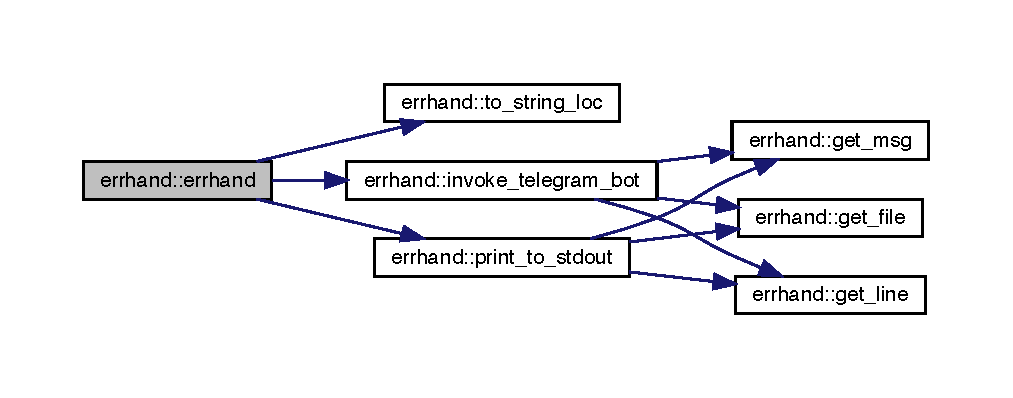
\includegraphics[width=350pt]{classerrhand_a69afd61e0ebf5ee9d35f297dc2d5c086_cgraph}
\end{center}
\end{figure}


\subsubsection{Member Function Documentation}
\mbox{\Hypertarget{classerrhand_a1556ee8d0aaefeea3bbab73f7ae50914}\label{classerrhand_a1556ee8d0aaefeea3bbab73f7ae50914}} 
\index{errhand@{errhand}!get\+\_\+file@{get\+\_\+file}}
\index{get\+\_\+file@{get\+\_\+file}!errhand@{errhand}}
\paragraph{\texorpdfstring{get\+\_\+file()}{get\_file()}}
{\footnotesize\ttfamily std\+::string errhand\+::get\+\_\+file (\begin{DoxyParamCaption}{ }\end{DoxyParamCaption}) const\hspace{0.3cm}{\ttfamily [inline]}}

Here is the caller graph for this function\+:\nopagebreak
\begin{figure}[H]
\begin{center}
\leavevmode
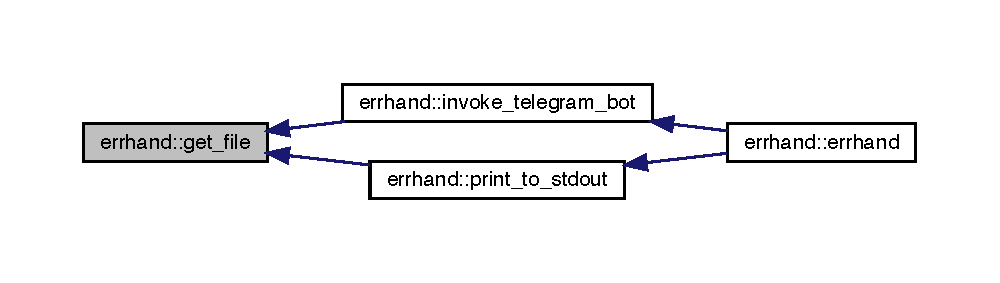
\includegraphics[width=350pt]{classerrhand_a1556ee8d0aaefeea3bbab73f7ae50914_icgraph}
\end{center}
\end{figure}
\mbox{\Hypertarget{classerrhand_a258f97d84476b21efc38827cda3e5889}\label{classerrhand_a258f97d84476b21efc38827cda3e5889}} 
\index{errhand@{errhand}!get\+\_\+line@{get\+\_\+line}}
\index{get\+\_\+line@{get\+\_\+line}!errhand@{errhand}}
\paragraph{\texorpdfstring{get\+\_\+line()}{get\_line()}}
{\footnotesize\ttfamily size\+\_\+t errhand\+::get\+\_\+line (\begin{DoxyParamCaption}{ }\end{DoxyParamCaption}) const\hspace{0.3cm}{\ttfamily [inline]}}

Here is the caller graph for this function\+:\nopagebreak
\begin{figure}[H]
\begin{center}
\leavevmode
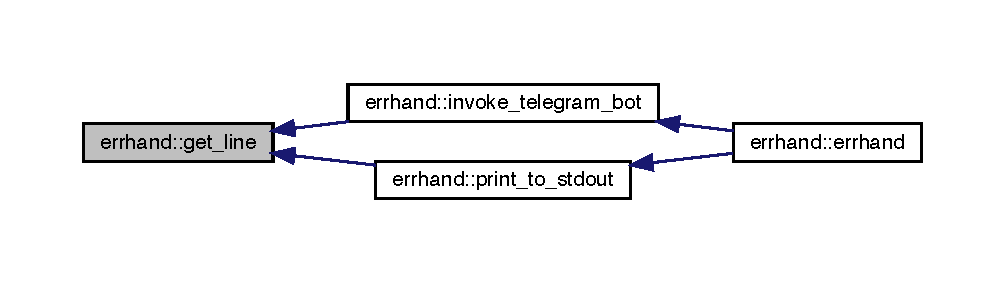
\includegraphics[width=350pt]{classerrhand_a258f97d84476b21efc38827cda3e5889_icgraph}
\end{center}
\end{figure}
\mbox{\Hypertarget{classerrhand_a524dfc6821f703329d8801dd3298f33f}\label{classerrhand_a524dfc6821f703329d8801dd3298f33f}} 
\index{errhand@{errhand}!get\+\_\+msg@{get\+\_\+msg}}
\index{get\+\_\+msg@{get\+\_\+msg}!errhand@{errhand}}
\paragraph{\texorpdfstring{get\+\_\+msg()}{get\_msg()}}
{\footnotesize\ttfamily std\+::string errhand\+::get\+\_\+msg (\begin{DoxyParamCaption}{ }\end{DoxyParamCaption}) const\hspace{0.3cm}{\ttfamily [inline]}}

Here is the caller graph for this function\+:\nopagebreak
\begin{figure}[H]
\begin{center}
\leavevmode
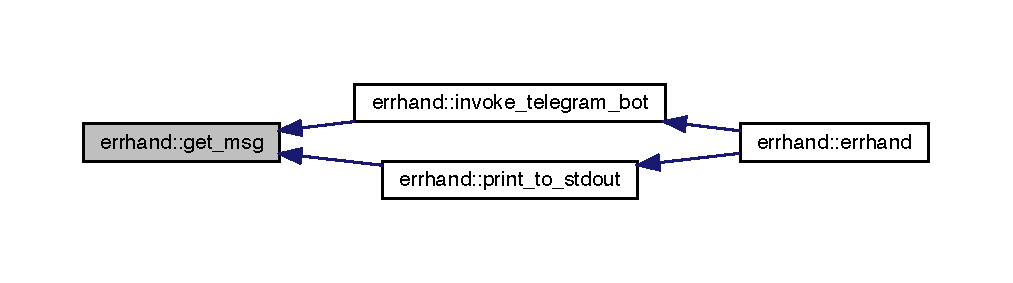
\includegraphics[width=350pt]{classerrhand_a524dfc6821f703329d8801dd3298f33f_icgraph}
\end{center}
\end{figure}
\mbox{\Hypertarget{classerrhand_adbc86e81b391a68d2bf9a13529c977d3}\label{classerrhand_adbc86e81b391a68d2bf9a13529c977d3}} 
\index{errhand@{errhand}!invoke\+\_\+telegram\+\_\+bot@{invoke\+\_\+telegram\+\_\+bot}}
\index{invoke\+\_\+telegram\+\_\+bot@{invoke\+\_\+telegram\+\_\+bot}!errhand@{errhand}}
\paragraph{\texorpdfstring{invoke\+\_\+telegram\+\_\+bot()}{invoke\_telegram\_bot()}}
{\footnotesize\ttfamily void errhand\+::invoke\+\_\+telegram\+\_\+bot (\begin{DoxyParamCaption}{ }\end{DoxyParamCaption})\hspace{0.3cm}{\ttfamily [inline]}}

Here is the call graph for this function\+:\nopagebreak
\begin{figure}[H]
\begin{center}
\leavevmode
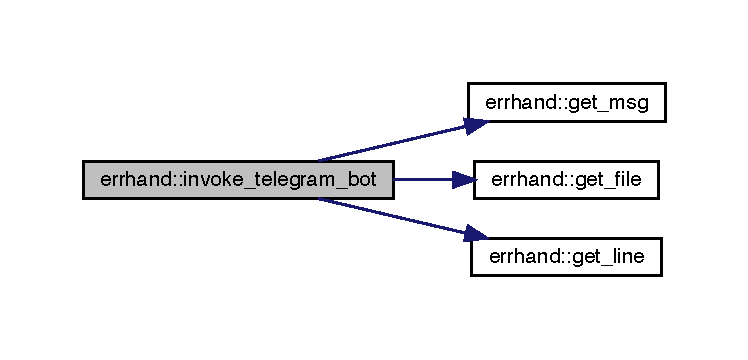
\includegraphics[width=350pt]{classerrhand_adbc86e81b391a68d2bf9a13529c977d3_cgraph}
\end{center}
\end{figure}
Here is the caller graph for this function\+:\nopagebreak
\begin{figure}[H]
\begin{center}
\leavevmode
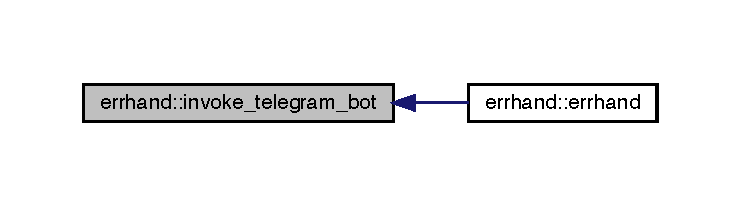
\includegraphics[width=350pt]{classerrhand_adbc86e81b391a68d2bf9a13529c977d3_icgraph}
\end{center}
\end{figure}
\mbox{\Hypertarget{classerrhand_a5b4d8a74f1d0c6842526dc8b54e38dc2}\label{classerrhand_a5b4d8a74f1d0c6842526dc8b54e38dc2}} 
\index{errhand@{errhand}!print\+\_\+to\+\_\+stdout@{print\+\_\+to\+\_\+stdout}}
\index{print\+\_\+to\+\_\+stdout@{print\+\_\+to\+\_\+stdout}!errhand@{errhand}}
\paragraph{\texorpdfstring{print\+\_\+to\+\_\+stdout()}{print\_to\_stdout()}}
{\footnotesize\ttfamily void errhand\+::print\+\_\+to\+\_\+stdout (\begin{DoxyParamCaption}{ }\end{DoxyParamCaption})\hspace{0.3cm}{\ttfamily [inline]}}

Here is the call graph for this function\+:\nopagebreak
\begin{figure}[H]
\begin{center}
\leavevmode
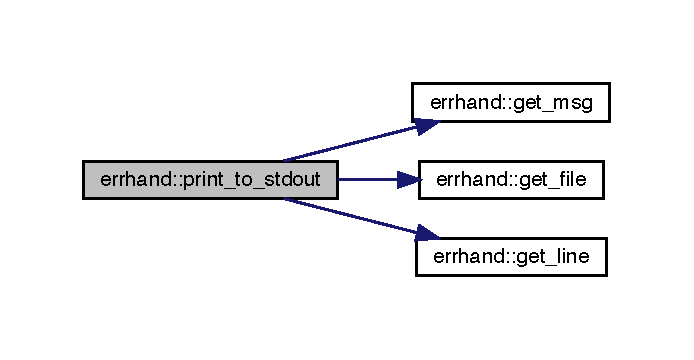
\includegraphics[width=333pt]{classerrhand_a5b4d8a74f1d0c6842526dc8b54e38dc2_cgraph}
\end{center}
\end{figure}
Here is the caller graph for this function\+:\nopagebreak
\begin{figure}[H]
\begin{center}
\leavevmode
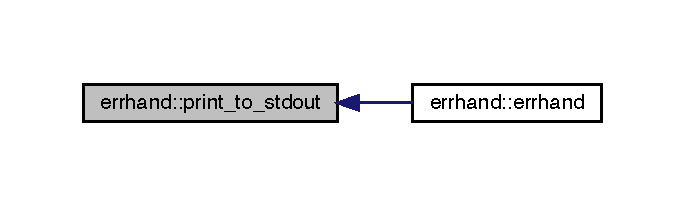
\includegraphics[width=329pt]{classerrhand_a5b4d8a74f1d0c6842526dc8b54e38dc2_icgraph}
\end{center}
\end{figure}
\mbox{\Hypertarget{classerrhand_a930df1c197154853159683cb2ad55369}\label{classerrhand_a930df1c197154853159683cb2ad55369}} 
\index{errhand@{errhand}!to\+\_\+string\+\_\+loc@{to\+\_\+string\+\_\+loc}}
\index{to\+\_\+string\+\_\+loc@{to\+\_\+string\+\_\+loc}!errhand@{errhand}}
\paragraph{\texorpdfstring{to\+\_\+string\+\_\+loc()}{to\_string\_loc()}}
{\footnotesize\ttfamily std\+::string errhand\+::to\+\_\+string\+\_\+loc (\begin{DoxyParamCaption}\item[{const char $\ast$}]{obj }\end{DoxyParamCaption})\hspace{0.3cm}{\ttfamily [inline]}}

Here is the caller graph for this function\+:\nopagebreak
\begin{figure}[H]
\begin{center}
\leavevmode
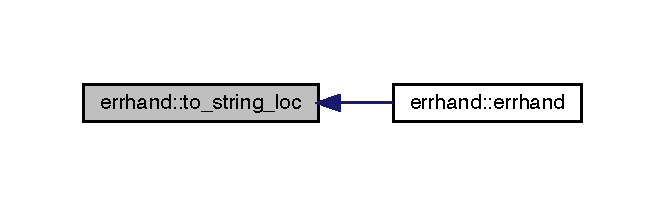
\includegraphics[width=319pt]{classerrhand_a930df1c197154853159683cb2ad55369_icgraph}
\end{center}
\end{figure}


\subsubsection{Member Data Documentation}
\mbox{\Hypertarget{classerrhand_a2baa975c76a80afce9c97575c549058c}\label{classerrhand_a2baa975c76a80afce9c97575c549058c}} 
\index{errhand@{errhand}!err\+\_\+msg@{err\+\_\+msg}}
\index{err\+\_\+msg@{err\+\_\+msg}!errhand@{errhand}}
\paragraph{\texorpdfstring{err\+\_\+msg}{err\_msg}}
{\footnotesize\ttfamily std\+::string errhand\+::err\+\_\+msg\hspace{0.3cm}{\ttfamily [private]}}

\mbox{\Hypertarget{classerrhand_aed73d7a312fae4b4387d8d2487277a74}\label{classerrhand_aed73d7a312fae4b4387d8d2487277a74}} 
\index{errhand@{errhand}!file@{file}}
\index{file@{file}!errhand@{errhand}}
\paragraph{\texorpdfstring{file}{file}}
{\footnotesize\ttfamily std\+::string errhand\+::file\hspace{0.3cm}{\ttfamily [private]}}

\mbox{\Hypertarget{classerrhand_a3ddc204c758b97e7d1550019e4513f3b}\label{classerrhand_a3ddc204c758b97e7d1550019e4513f3b}} 
\index{errhand@{errhand}!line@{line}}
\index{line@{line}!errhand@{errhand}}
\paragraph{\texorpdfstring{line}{line}}
{\footnotesize\ttfamily size\+\_\+t errhand\+::line\hspace{0.3cm}{\ttfamily [private]}}



The documentation for this class was generated from the following file\+:\begin{DoxyCompactItemize}
\item 
\mbox{\hyperlink{errhand_8h}{errhand.\+h}}\end{DoxyCompactItemize}

\hypertarget{struct_space_h_1_1_ext_vel_dep_force}{}\section{SpaceH\+:\+:Ext\+Vel\+Dep\+Force$<$ Ext\+Force, Dtype, Array\+Size $>$ Struct Template Reference}
\label{struct_space_h_1_1_ext_vel_dep_force}\index{Space\+H\+::\+Ext\+Vel\+Dep\+Force$<$ Ext\+Force, Dtype, Array\+Size $>$@{Space\+H\+::\+Ext\+Vel\+Dep\+Force$<$ Ext\+Force, Dtype, Array\+Size $>$}}


{\ttfamily \#include $<$force.\+h$>$}



Inheritance diagram for SpaceH\+:\+:Ext\+Vel\+Dep\+Force$<$ Ext\+Force, Dtype, Array\+Size $>$\+:\nopagebreak
\begin{figure}[H]
\begin{center}
\leavevmode
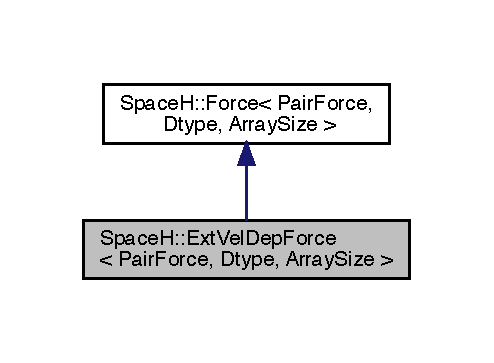
\includegraphics[width=237pt]{struct_space_h_1_1_ext_vel_dep_force__inherit__graph}
\end{center}
\end{figure}


Collaboration diagram for SpaceH\+:\+:Ext\+Vel\+Dep\+Force$<$ Ext\+Force, Dtype, Array\+Size $>$\+:\nopagebreak
\begin{figure}[H]
\begin{center}
\leavevmode
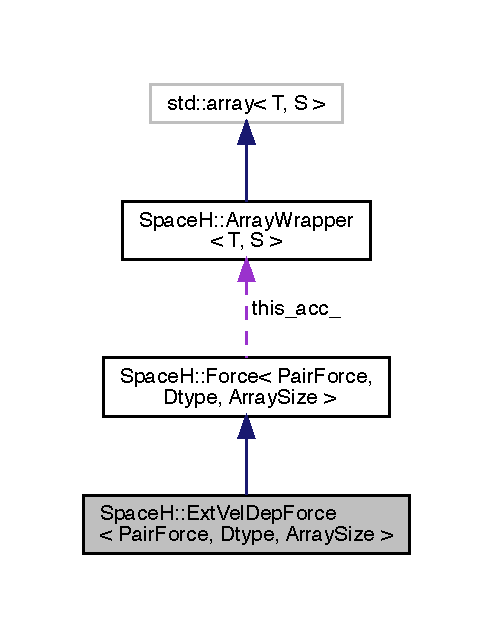
\includegraphics[width=237pt]{struct_space_h_1_1_ext_vel_dep_force__coll__graph}
\end{center}
\end{figure}
\subsection*{Public Types}
\begin{DoxyCompactItemize}
\item 
using \mbox{\hyperlink{struct_space_h_1_1_ext_vel_dep_force_a92ddc0ad1001e17ef8b4f870be20cada}{Base}} = \mbox{\hyperlink{struct_space_h_1_1_force}{Force}}$<$ Ext\+Force, Dtype, Array\+Size $>$
\item 
using \mbox{\hyperlink{struct_space_h_1_1_ext_vel_dep_force_ace51228267cd84b498bef72f6a06b727}{type}} = typename \mbox{\hyperlink{struct_space_h_1_1_force_a151c6ae1ec7ad87825c2b6cc74aee5f2}{Base\+::type}}
\item 
using \mbox{\hyperlink{struct_space_h_1_1_ext_vel_dep_force_afb0d9418e7236855d8cd8ce883493c27}{Scalar\+Array}} = typename type\+::\+Scalar\+Array
\item 
using \mbox{\hyperlink{struct_space_h_1_1_ext_vel_dep_force_ac2320cdd3fdaad369c901e79ded11d31}{Vector\+Array}} = typename type\+::\+Vector\+Array
\end{DoxyCompactItemize}
\subsection*{Public Member Functions}
\begin{DoxyCompactItemize}
\item 
void \mbox{\hyperlink{struct_space_h_1_1_ext_vel_dep_force_a58775894138f5ebd1d7d7460183f6c1e}{calcu\+Acc}} (const \mbox{\hyperlink{struct_space_h_1_1_ext_vel_dep_force_afb0d9418e7236855d8cd8ce883493c27}{Scalar\+Array}} \&mass, const \mbox{\hyperlink{struct_space_h_1_1_ext_vel_dep_force_ac2320cdd3fdaad369c901e79ded11d31}{Vector\+Array}} \&pos, const \mbox{\hyperlink{struct_space_h_1_1_ext_vel_dep_force_ac2320cdd3fdaad369c901e79ded11d31}{Vector\+Array}} \&vel)
\end{DoxyCompactItemize}
\subsection*{Additional Inherited Members}


\subsection{Member Typedef Documentation}
\mbox{\Hypertarget{struct_space_h_1_1_ext_vel_dep_force_a92ddc0ad1001e17ef8b4f870be20cada}\label{struct_space_h_1_1_ext_vel_dep_force_a92ddc0ad1001e17ef8b4f870be20cada}} 
\index{Space\+H\+::\+Ext\+Vel\+Dep\+Force@{Space\+H\+::\+Ext\+Vel\+Dep\+Force}!Base@{Base}}
\index{Base@{Base}!Space\+H\+::\+Ext\+Vel\+Dep\+Force@{Space\+H\+::\+Ext\+Vel\+Dep\+Force}}
\subsubsection{\texorpdfstring{Base}{Base}}
{\footnotesize\ttfamily template$<$typename Ext\+Force, typename Dtype, size\+\_\+t Array\+Size$>$ \\
using \mbox{\hyperlink{struct_space_h_1_1_ext_vel_dep_force}{Space\+H\+::\+Ext\+Vel\+Dep\+Force}}$<$ Ext\+Force, Dtype, Array\+Size $>$\+::\mbox{\hyperlink{struct_space_h_1_1_ext_vel_dep_force_a92ddc0ad1001e17ef8b4f870be20cada}{Base}} =  \mbox{\hyperlink{struct_space_h_1_1_force}{Force}}$<$Ext\+Force, Dtype, Array\+Size$>$}

\mbox{\Hypertarget{struct_space_h_1_1_ext_vel_dep_force_afb0d9418e7236855d8cd8ce883493c27}\label{struct_space_h_1_1_ext_vel_dep_force_afb0d9418e7236855d8cd8ce883493c27}} 
\index{Space\+H\+::\+Ext\+Vel\+Dep\+Force@{Space\+H\+::\+Ext\+Vel\+Dep\+Force}!Scalar\+Array@{Scalar\+Array}}
\index{Scalar\+Array@{Scalar\+Array}!Space\+H\+::\+Ext\+Vel\+Dep\+Force@{Space\+H\+::\+Ext\+Vel\+Dep\+Force}}
\subsubsection{\texorpdfstring{Scalar\+Array}{ScalarArray}}
{\footnotesize\ttfamily template$<$typename Ext\+Force, typename Dtype, size\+\_\+t Array\+Size$>$ \\
using \mbox{\hyperlink{struct_space_h_1_1_ext_vel_dep_force}{Space\+H\+::\+Ext\+Vel\+Dep\+Force}}$<$ Ext\+Force, Dtype, Array\+Size $>$\+::\mbox{\hyperlink{struct_space_h_1_1_ext_vel_dep_force_afb0d9418e7236855d8cd8ce883493c27}{Scalar\+Array}} =  typename type\+::\+Scalar\+Array}

\mbox{\Hypertarget{struct_space_h_1_1_ext_vel_dep_force_ace51228267cd84b498bef72f6a06b727}\label{struct_space_h_1_1_ext_vel_dep_force_ace51228267cd84b498bef72f6a06b727}} 
\index{Space\+H\+::\+Ext\+Vel\+Dep\+Force@{Space\+H\+::\+Ext\+Vel\+Dep\+Force}!type@{type}}
\index{type@{type}!Space\+H\+::\+Ext\+Vel\+Dep\+Force@{Space\+H\+::\+Ext\+Vel\+Dep\+Force}}
\subsubsection{\texorpdfstring{type}{type}}
{\footnotesize\ttfamily template$<$typename Ext\+Force, typename Dtype, size\+\_\+t Array\+Size$>$ \\
using \mbox{\hyperlink{struct_space_h_1_1_ext_vel_dep_force}{Space\+H\+::\+Ext\+Vel\+Dep\+Force}}$<$ Ext\+Force, Dtype, Array\+Size $>$\+::\mbox{\hyperlink{struct_space_h_1_1_ext_vel_dep_force_ace51228267cd84b498bef72f6a06b727}{type}} =  typename \mbox{\hyperlink{struct_space_h_1_1_force_a151c6ae1ec7ad87825c2b6cc74aee5f2}{Base\+::type}}}

\mbox{\Hypertarget{struct_space_h_1_1_ext_vel_dep_force_ac2320cdd3fdaad369c901e79ded11d31}\label{struct_space_h_1_1_ext_vel_dep_force_ac2320cdd3fdaad369c901e79ded11d31}} 
\index{Space\+H\+::\+Ext\+Vel\+Dep\+Force@{Space\+H\+::\+Ext\+Vel\+Dep\+Force}!Vector\+Array@{Vector\+Array}}
\index{Vector\+Array@{Vector\+Array}!Space\+H\+::\+Ext\+Vel\+Dep\+Force@{Space\+H\+::\+Ext\+Vel\+Dep\+Force}}
\subsubsection{\texorpdfstring{Vector\+Array}{VectorArray}}
{\footnotesize\ttfamily template$<$typename Ext\+Force, typename Dtype, size\+\_\+t Array\+Size$>$ \\
using \mbox{\hyperlink{struct_space_h_1_1_ext_vel_dep_force}{Space\+H\+::\+Ext\+Vel\+Dep\+Force}}$<$ Ext\+Force, Dtype, Array\+Size $>$\+::\mbox{\hyperlink{struct_space_h_1_1_ext_vel_dep_force_ac2320cdd3fdaad369c901e79ded11d31}{Vector\+Array}} =  typename type\+::\+Vector\+Array}



\subsection{Member Function Documentation}
\mbox{\Hypertarget{struct_space_h_1_1_ext_vel_dep_force_a58775894138f5ebd1d7d7460183f6c1e}\label{struct_space_h_1_1_ext_vel_dep_force_a58775894138f5ebd1d7d7460183f6c1e}} 
\index{Space\+H\+::\+Ext\+Vel\+Dep\+Force@{Space\+H\+::\+Ext\+Vel\+Dep\+Force}!calcu\+Acc@{calcu\+Acc}}
\index{calcu\+Acc@{calcu\+Acc}!Space\+H\+::\+Ext\+Vel\+Dep\+Force@{Space\+H\+::\+Ext\+Vel\+Dep\+Force}}
\subsubsection{\texorpdfstring{calcu\+Acc()}{calcuAcc()}}
{\footnotesize\ttfamily template$<$typename Ext\+Force, typename Dtype, size\+\_\+t Array\+Size$>$ \\
void \mbox{\hyperlink{struct_space_h_1_1_ext_vel_dep_force}{Space\+H\+::\+Ext\+Vel\+Dep\+Force}}$<$ Ext\+Force, Dtype, Array\+Size $>$\+::calcu\+Acc (\begin{DoxyParamCaption}\item[{const \mbox{\hyperlink{struct_space_h_1_1_ext_vel_dep_force_afb0d9418e7236855d8cd8ce883493c27}{Scalar\+Array}} \&}]{mass,  }\item[{const \mbox{\hyperlink{struct_space_h_1_1_ext_vel_dep_force_ac2320cdd3fdaad369c901e79ded11d31}{Vector\+Array}} \&}]{pos,  }\item[{const \mbox{\hyperlink{struct_space_h_1_1_ext_vel_dep_force_ac2320cdd3fdaad369c901e79ded11d31}{Vector\+Array}} \&}]{vel }\end{DoxyParamCaption})\hspace{0.3cm}{\ttfamily [inline]}}

Here is the caller graph for this function\+:
\nopagebreak
\begin{figure}[H]
\begin{center}
\leavevmode
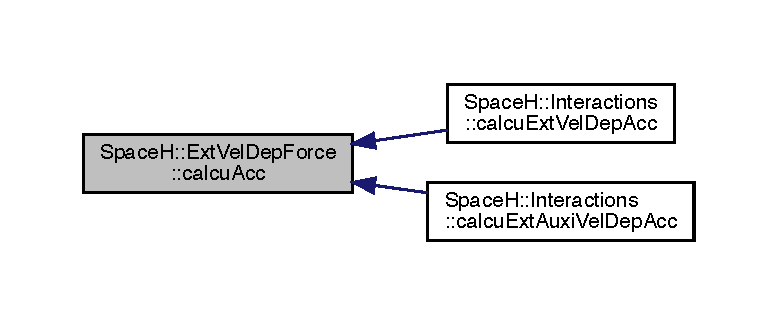
\includegraphics[width=350pt]{struct_space_h_1_1_ext_vel_dep_force_a58775894138f5ebd1d7d7460183f6c1e_icgraph}
\end{center}
\end{figure}


The documentation for this struct was generated from the following file\+:\begin{DoxyCompactItemize}
\item 
interaction/\mbox{\hyperlink{force_8h}{force.\+h}}\end{DoxyCompactItemize}

\hypertarget{struct_space_h_1_1_ext_vel_indep_force}{}\section{SpaceH\+:\+:Ext\+Vel\+Indep\+Force$<$ Ext\+Force, Dtype, Array\+Size $>$ Struct Template Reference}
\label{struct_space_h_1_1_ext_vel_indep_force}\index{Space\+H\+::\+Ext\+Vel\+Indep\+Force$<$ Ext\+Force, Dtype, Array\+Size $>$@{Space\+H\+::\+Ext\+Vel\+Indep\+Force$<$ Ext\+Force, Dtype, Array\+Size $>$}}


{\ttfamily \#include $<$force.\+h$>$}



Inheritance diagram for SpaceH\+:\+:Ext\+Vel\+Indep\+Force$<$ Ext\+Force, Dtype, Array\+Size $>$\+:\nopagebreak
\begin{figure}[H]
\begin{center}
\leavevmode
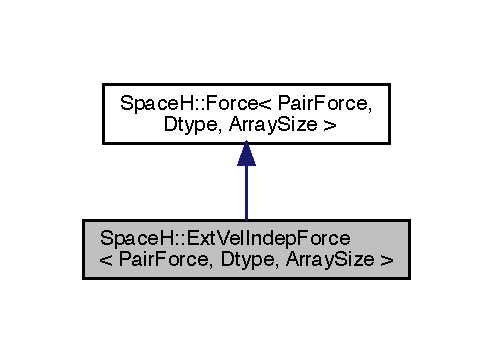
\includegraphics[width=237pt]{struct_space_h_1_1_ext_vel_indep_force__inherit__graph}
\end{center}
\end{figure}


Collaboration diagram for SpaceH\+:\+:Ext\+Vel\+Indep\+Force$<$ Ext\+Force, Dtype, Array\+Size $>$\+:\nopagebreak
\begin{figure}[H]
\begin{center}
\leavevmode
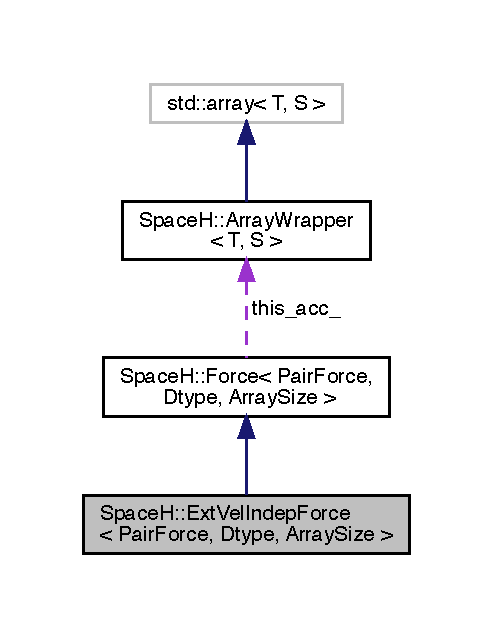
\includegraphics[width=237pt]{struct_space_h_1_1_ext_vel_indep_force__coll__graph}
\end{center}
\end{figure}
\subsection*{Public Types}
\begin{DoxyCompactItemize}
\item 
using \mbox{\hyperlink{struct_space_h_1_1_ext_vel_indep_force_acf786913cd012bc90bb02f9ae1f87e91}{Base}} = \mbox{\hyperlink{struct_space_h_1_1_force}{Force}}$<$ Ext\+Force, Dtype, Array\+Size $>$
\item 
using \mbox{\hyperlink{struct_space_h_1_1_ext_vel_indep_force_a6db7150bace18b57cb059989c7f29e50}{type}} = typename \mbox{\hyperlink{struct_space_h_1_1_force_a151c6ae1ec7ad87825c2b6cc74aee5f2}{Base\+::type}}
\item 
using \mbox{\hyperlink{struct_space_h_1_1_ext_vel_indep_force_afe9c9f6c747f7b82f5e1058f5df2f2af}{Scalar\+Array}} = typename type\+::\+Scalar\+Array
\item 
using \mbox{\hyperlink{struct_space_h_1_1_ext_vel_indep_force_ae9d2ecd856cbcfa1cc848003a8450adf}{Vector\+Array}} = typename type\+::\+Vector\+Array
\end{DoxyCompactItemize}
\subsection*{Public Member Functions}
\begin{DoxyCompactItemize}
\item 
void \mbox{\hyperlink{struct_space_h_1_1_ext_vel_indep_force_ade2a9eececdb0833213048c1e73c7756}{calcu\+Acc}} (const \mbox{\hyperlink{struct_space_h_1_1_ext_vel_indep_force_afe9c9f6c747f7b82f5e1058f5df2f2af}{Scalar\+Array}} \&mass, const \mbox{\hyperlink{struct_space_h_1_1_ext_vel_indep_force_ae9d2ecd856cbcfa1cc848003a8450adf}{Vector\+Array}} \&pos)
\end{DoxyCompactItemize}
\subsection*{Additional Inherited Members}


\subsection{Member Typedef Documentation}
\mbox{\Hypertarget{struct_space_h_1_1_ext_vel_indep_force_acf786913cd012bc90bb02f9ae1f87e91}\label{struct_space_h_1_1_ext_vel_indep_force_acf786913cd012bc90bb02f9ae1f87e91}} 
\index{Space\+H\+::\+Ext\+Vel\+Indep\+Force@{Space\+H\+::\+Ext\+Vel\+Indep\+Force}!Base@{Base}}
\index{Base@{Base}!Space\+H\+::\+Ext\+Vel\+Indep\+Force@{Space\+H\+::\+Ext\+Vel\+Indep\+Force}}
\subsubsection{\texorpdfstring{Base}{Base}}
{\footnotesize\ttfamily template$<$typename Ext\+Force, typename Dtype, size\+\_\+t Array\+Size$>$ \\
using \mbox{\hyperlink{struct_space_h_1_1_ext_vel_indep_force}{Space\+H\+::\+Ext\+Vel\+Indep\+Force}}$<$ Ext\+Force, Dtype, Array\+Size $>$\+::\mbox{\hyperlink{struct_space_h_1_1_ext_vel_indep_force_acf786913cd012bc90bb02f9ae1f87e91}{Base}} =  \mbox{\hyperlink{struct_space_h_1_1_force}{Force}}$<$Ext\+Force, Dtype, Array\+Size$>$}

\mbox{\Hypertarget{struct_space_h_1_1_ext_vel_indep_force_afe9c9f6c747f7b82f5e1058f5df2f2af}\label{struct_space_h_1_1_ext_vel_indep_force_afe9c9f6c747f7b82f5e1058f5df2f2af}} 
\index{Space\+H\+::\+Ext\+Vel\+Indep\+Force@{Space\+H\+::\+Ext\+Vel\+Indep\+Force}!Scalar\+Array@{Scalar\+Array}}
\index{Scalar\+Array@{Scalar\+Array}!Space\+H\+::\+Ext\+Vel\+Indep\+Force@{Space\+H\+::\+Ext\+Vel\+Indep\+Force}}
\subsubsection{\texorpdfstring{Scalar\+Array}{ScalarArray}}
{\footnotesize\ttfamily template$<$typename Ext\+Force, typename Dtype, size\+\_\+t Array\+Size$>$ \\
using \mbox{\hyperlink{struct_space_h_1_1_ext_vel_indep_force}{Space\+H\+::\+Ext\+Vel\+Indep\+Force}}$<$ Ext\+Force, Dtype, Array\+Size $>$\+::\mbox{\hyperlink{struct_space_h_1_1_ext_vel_indep_force_afe9c9f6c747f7b82f5e1058f5df2f2af}{Scalar\+Array}} =  typename type\+::\+Scalar\+Array}

\mbox{\Hypertarget{struct_space_h_1_1_ext_vel_indep_force_a6db7150bace18b57cb059989c7f29e50}\label{struct_space_h_1_1_ext_vel_indep_force_a6db7150bace18b57cb059989c7f29e50}} 
\index{Space\+H\+::\+Ext\+Vel\+Indep\+Force@{Space\+H\+::\+Ext\+Vel\+Indep\+Force}!type@{type}}
\index{type@{type}!Space\+H\+::\+Ext\+Vel\+Indep\+Force@{Space\+H\+::\+Ext\+Vel\+Indep\+Force}}
\subsubsection{\texorpdfstring{type}{type}}
{\footnotesize\ttfamily template$<$typename Ext\+Force, typename Dtype, size\+\_\+t Array\+Size$>$ \\
using \mbox{\hyperlink{struct_space_h_1_1_ext_vel_indep_force}{Space\+H\+::\+Ext\+Vel\+Indep\+Force}}$<$ Ext\+Force, Dtype, Array\+Size $>$\+::\mbox{\hyperlink{struct_space_h_1_1_ext_vel_indep_force_a6db7150bace18b57cb059989c7f29e50}{type}} =  typename \mbox{\hyperlink{struct_space_h_1_1_force_a151c6ae1ec7ad87825c2b6cc74aee5f2}{Base\+::type}}}

\mbox{\Hypertarget{struct_space_h_1_1_ext_vel_indep_force_ae9d2ecd856cbcfa1cc848003a8450adf}\label{struct_space_h_1_1_ext_vel_indep_force_ae9d2ecd856cbcfa1cc848003a8450adf}} 
\index{Space\+H\+::\+Ext\+Vel\+Indep\+Force@{Space\+H\+::\+Ext\+Vel\+Indep\+Force}!Vector\+Array@{Vector\+Array}}
\index{Vector\+Array@{Vector\+Array}!Space\+H\+::\+Ext\+Vel\+Indep\+Force@{Space\+H\+::\+Ext\+Vel\+Indep\+Force}}
\subsubsection{\texorpdfstring{Vector\+Array}{VectorArray}}
{\footnotesize\ttfamily template$<$typename Ext\+Force, typename Dtype, size\+\_\+t Array\+Size$>$ \\
using \mbox{\hyperlink{struct_space_h_1_1_ext_vel_indep_force}{Space\+H\+::\+Ext\+Vel\+Indep\+Force}}$<$ Ext\+Force, Dtype, Array\+Size $>$\+::\mbox{\hyperlink{struct_space_h_1_1_ext_vel_indep_force_ae9d2ecd856cbcfa1cc848003a8450adf}{Vector\+Array}} =  typename type\+::\+Vector\+Array}



\subsection{Member Function Documentation}
\mbox{\Hypertarget{struct_space_h_1_1_ext_vel_indep_force_ade2a9eececdb0833213048c1e73c7756}\label{struct_space_h_1_1_ext_vel_indep_force_ade2a9eececdb0833213048c1e73c7756}} 
\index{Space\+H\+::\+Ext\+Vel\+Indep\+Force@{Space\+H\+::\+Ext\+Vel\+Indep\+Force}!calcu\+Acc@{calcu\+Acc}}
\index{calcu\+Acc@{calcu\+Acc}!Space\+H\+::\+Ext\+Vel\+Indep\+Force@{Space\+H\+::\+Ext\+Vel\+Indep\+Force}}
\subsubsection{\texorpdfstring{calcu\+Acc()}{calcuAcc()}}
{\footnotesize\ttfamily template$<$typename Ext\+Force, typename Dtype, size\+\_\+t Array\+Size$>$ \\
void \mbox{\hyperlink{struct_space_h_1_1_ext_vel_indep_force}{Space\+H\+::\+Ext\+Vel\+Indep\+Force}}$<$ Ext\+Force, Dtype, Array\+Size $>$\+::calcu\+Acc (\begin{DoxyParamCaption}\item[{const \mbox{\hyperlink{struct_space_h_1_1_ext_vel_indep_force_afe9c9f6c747f7b82f5e1058f5df2f2af}{Scalar\+Array}} \&}]{mass,  }\item[{const \mbox{\hyperlink{struct_space_h_1_1_ext_vel_indep_force_ae9d2ecd856cbcfa1cc848003a8450adf}{Vector\+Array}} \&}]{pos }\end{DoxyParamCaption})\hspace{0.3cm}{\ttfamily [inline]}}

Here is the caller graph for this function\+:
\nopagebreak
\begin{figure}[H]
\begin{center}
\leavevmode
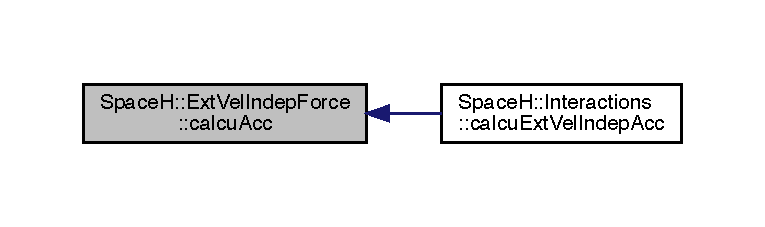
\includegraphics[width=350pt]{struct_space_h_1_1_ext_vel_indep_force_ade2a9eececdb0833213048c1e73c7756_icgraph}
\end{center}
\end{figure}


The documentation for this struct was generated from the following file\+:\begin{DoxyCompactItemize}
\item 
interaction/\mbox{\hyperlink{force_8h}{force.\+h}}\end{DoxyCompactItemize}

\hypertarget{struct_space_h_1_1_force}{}\section{SpaceH\+:\+:Force$<$ Forcefunc, Dtype, Array\+Size $>$ Struct Template Reference}
\label{struct_space_h_1_1_force}\index{Space\+H\+::\+Force$<$ Forcefunc, Dtype, Array\+Size $>$@{Space\+H\+::\+Force$<$ Forcefunc, Dtype, Array\+Size $>$}}


{\ttfamily \#include $<$force.\+h$>$}



Collaboration diagram for SpaceH\+:\+:Force$<$ Forcefunc, Dtype, Array\+Size $>$\+:\nopagebreak
\begin{figure}[H]
\begin{center}
\leavevmode
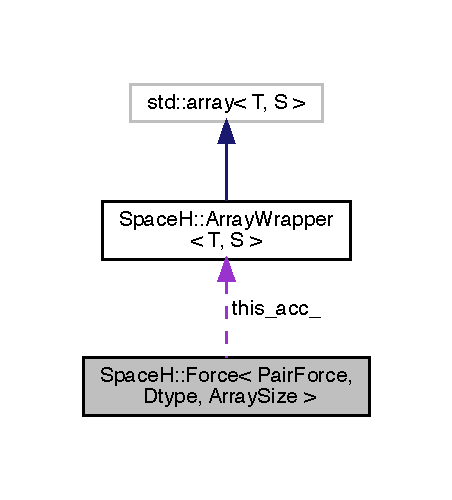
\includegraphics[width=217pt]{struct_space_h_1_1_force__coll__graph}
\end{center}
\end{figure}
\subsection*{Public Types}
\begin{DoxyCompactItemize}
\item 
using \mbox{\hyperlink{struct_space_h_1_1_force_a151c6ae1ec7ad87825c2b6cc74aee5f2}{type}} = \mbox{\hyperlink{struct_space_h_1_1_proto_type}{Space\+H\+::\+Proto\+Type}}$<$ Dtype, Array\+Size $>$
\item 
using \mbox{\hyperlink{struct_space_h_1_1_force_a7da326c7793f559bb39c73b6d0d01e39}{Vector}} = typename \mbox{\hyperlink{struct_space_h_1_1_proto_type_a316b81f4660b2b4fab14a8e1f23b6089}{type\+::\+Vector}}
\item 
using \mbox{\hyperlink{struct_space_h_1_1_force_aa58fd21903006c1d033713d04b4719f3}{Vector\+Array}} = typename \mbox{\hyperlink{struct_space_h_1_1_proto_type_a622b8e122b33bb4966a02299fb7b82d6}{type\+::\+Vector\+Array}}
\end{DoxyCompactItemize}
\subsection*{Public Member Functions}
\begin{DoxyCompactItemize}
\item 
void \mbox{\hyperlink{struct_space_h_1_1_force_a9f85a2d5e3e642c6e1121c591c19dded}{add\+Total}} (\mbox{\hyperlink{struct_space_h_1_1_force_aa58fd21903006c1d033713d04b4719f3}{Vector\+Array}} \&\mbox{\hyperlink{struct_space_h_1_1_force_ac4f8ce97d4513859ad94064ed35ab300}{acc}})
\item 
const \mbox{\hyperlink{struct_space_h_1_1_force_aa58fd21903006c1d033713d04b4719f3}{Vector\+Array}} \& \mbox{\hyperlink{struct_space_h_1_1_force_ac4f8ce97d4513859ad94064ed35ab300}{acc}} () const
\item 
const \mbox{\hyperlink{struct_space_h_1_1_force_a7da326c7793f559bb39c73b6d0d01e39}{Vector}} \& \mbox{\hyperlink{struct_space_h_1_1_force_abff837e46b01461762054d79ebee0fb8}{acc}} (size\+\_\+t i) const
\item 
void \mbox{\hyperlink{struct_space_h_1_1_force_aa1a3ef23a57eb72d0004c4afe505eb0b}{check\+Array\+Size}} (size\+\_\+t size)
\end{DoxyCompactItemize}
\subsection*{Protected Attributes}
\begin{DoxyCompactItemize}
\item 
\mbox{\hyperlink{struct_space_h_1_1_force_aa58fd21903006c1d033713d04b4719f3}{Vector\+Array}} \mbox{\hyperlink{struct_space_h_1_1_force_a7e87abc40a345bc5e24bdf56ca32f045}{this\+\_\+acc\+\_\+}}
\item 
Forcefunc \mbox{\hyperlink{struct_space_h_1_1_force_a9d669e983d78f8bfa0e1a08dd27b6abb}{force\+\_\+}}
\end{DoxyCompactItemize}


\subsection{Member Typedef Documentation}
\mbox{\Hypertarget{struct_space_h_1_1_force_a151c6ae1ec7ad87825c2b6cc74aee5f2}\label{struct_space_h_1_1_force_a151c6ae1ec7ad87825c2b6cc74aee5f2}} 
\index{Space\+H\+::\+Force@{Space\+H\+::\+Force}!type@{type}}
\index{type@{type}!Space\+H\+::\+Force@{Space\+H\+::\+Force}}
\subsubsection{\texorpdfstring{type}{type}}
{\footnotesize\ttfamily template$<$typename Forcefunc, typename Dtype, size\+\_\+t Array\+Size$>$ \\
using \mbox{\hyperlink{struct_space_h_1_1_force}{Space\+H\+::\+Force}}$<$ Forcefunc, Dtype, Array\+Size $>$\+::\mbox{\hyperlink{struct_space_h_1_1_force_a151c6ae1ec7ad87825c2b6cc74aee5f2}{type}} =  \mbox{\hyperlink{struct_space_h_1_1_proto_type}{Space\+H\+::\+Proto\+Type}}$<$Dtype, Array\+Size$>$}

\mbox{\Hypertarget{struct_space_h_1_1_force_a7da326c7793f559bb39c73b6d0d01e39}\label{struct_space_h_1_1_force_a7da326c7793f559bb39c73b6d0d01e39}} 
\index{Space\+H\+::\+Force@{Space\+H\+::\+Force}!Vector@{Vector}}
\index{Vector@{Vector}!Space\+H\+::\+Force@{Space\+H\+::\+Force}}
\subsubsection{\texorpdfstring{Vector}{Vector}}
{\footnotesize\ttfamily template$<$typename Forcefunc, typename Dtype, size\+\_\+t Array\+Size$>$ \\
using \mbox{\hyperlink{struct_space_h_1_1_force}{Space\+H\+::\+Force}}$<$ Forcefunc, Dtype, Array\+Size $>$\+::\mbox{\hyperlink{struct_space_h_1_1_force_a7da326c7793f559bb39c73b6d0d01e39}{Vector}} =  typename \mbox{\hyperlink{struct_space_h_1_1_proto_type_a316b81f4660b2b4fab14a8e1f23b6089}{type\+::\+Vector}}}

\mbox{\Hypertarget{struct_space_h_1_1_force_aa58fd21903006c1d033713d04b4719f3}\label{struct_space_h_1_1_force_aa58fd21903006c1d033713d04b4719f3}} 
\index{Space\+H\+::\+Force@{Space\+H\+::\+Force}!Vector\+Array@{Vector\+Array}}
\index{Vector\+Array@{Vector\+Array}!Space\+H\+::\+Force@{Space\+H\+::\+Force}}
\subsubsection{\texorpdfstring{Vector\+Array}{VectorArray}}
{\footnotesize\ttfamily template$<$typename Forcefunc, typename Dtype, size\+\_\+t Array\+Size$>$ \\
using \mbox{\hyperlink{struct_space_h_1_1_force}{Space\+H\+::\+Force}}$<$ Forcefunc, Dtype, Array\+Size $>$\+::\mbox{\hyperlink{struct_space_h_1_1_force_aa58fd21903006c1d033713d04b4719f3}{Vector\+Array}} =  typename \mbox{\hyperlink{struct_space_h_1_1_proto_type_a622b8e122b33bb4966a02299fb7b82d6}{type\+::\+Vector\+Array}}}



\subsection{Member Function Documentation}
\mbox{\Hypertarget{struct_space_h_1_1_force_ac4f8ce97d4513859ad94064ed35ab300}\label{struct_space_h_1_1_force_ac4f8ce97d4513859ad94064ed35ab300}} 
\index{Space\+H\+::\+Force@{Space\+H\+::\+Force}!acc@{acc}}
\index{acc@{acc}!Space\+H\+::\+Force@{Space\+H\+::\+Force}}
\subsubsection{\texorpdfstring{acc()}{acc()}\hspace{0.1cm}{\footnotesize\ttfamily [1/2]}}
{\footnotesize\ttfamily template$<$typename Forcefunc, typename Dtype, size\+\_\+t Array\+Size$>$ \\
const \mbox{\hyperlink{struct_space_h_1_1_force_aa58fd21903006c1d033713d04b4719f3}{Vector\+Array}}\& \mbox{\hyperlink{struct_space_h_1_1_force}{Space\+H\+::\+Force}}$<$ Forcefunc, Dtype, Array\+Size $>$\+::acc (\begin{DoxyParamCaption}{ }\end{DoxyParamCaption}) const\hspace{0.3cm}{\ttfamily [inline]}}

Here is the caller graph for this function\+:
\nopagebreak
\begin{figure}[H]
\begin{center}
\leavevmode
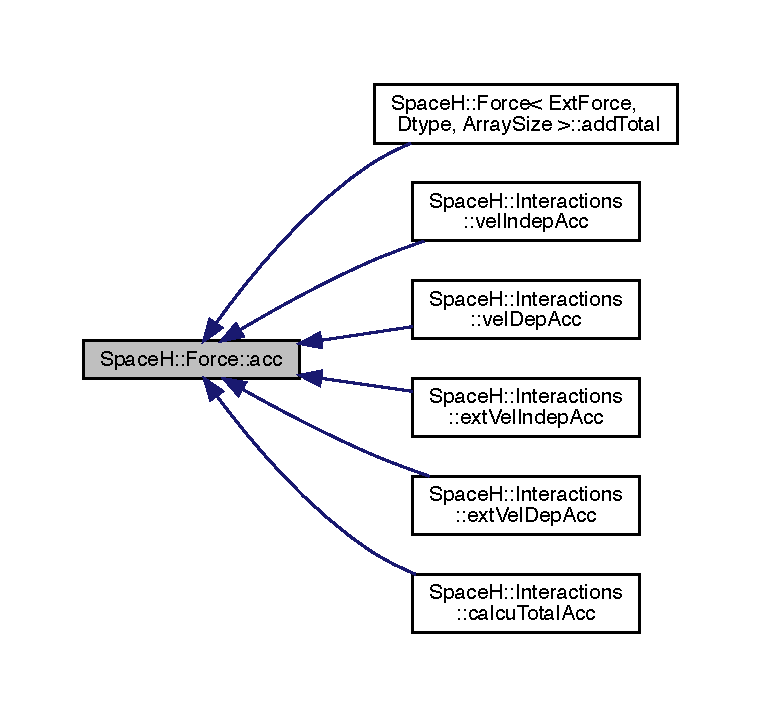
\includegraphics[width=350pt]{struct_space_h_1_1_force_ac4f8ce97d4513859ad94064ed35ab300_icgraph}
\end{center}
\end{figure}
\mbox{\Hypertarget{struct_space_h_1_1_force_abff837e46b01461762054d79ebee0fb8}\label{struct_space_h_1_1_force_abff837e46b01461762054d79ebee0fb8}} 
\index{Space\+H\+::\+Force@{Space\+H\+::\+Force}!acc@{acc}}
\index{acc@{acc}!Space\+H\+::\+Force@{Space\+H\+::\+Force}}
\subsubsection{\texorpdfstring{acc()}{acc()}\hspace{0.1cm}{\footnotesize\ttfamily [2/2]}}
{\footnotesize\ttfamily template$<$typename Forcefunc, typename Dtype, size\+\_\+t Array\+Size$>$ \\
const \mbox{\hyperlink{struct_space_h_1_1_force_a7da326c7793f559bb39c73b6d0d01e39}{Vector}}\& \mbox{\hyperlink{struct_space_h_1_1_force}{Space\+H\+::\+Force}}$<$ Forcefunc, Dtype, Array\+Size $>$\+::acc (\begin{DoxyParamCaption}\item[{size\+\_\+t}]{i }\end{DoxyParamCaption}) const\hspace{0.3cm}{\ttfamily [inline]}}

\mbox{\Hypertarget{struct_space_h_1_1_force_a9f85a2d5e3e642c6e1121c591c19dded}\label{struct_space_h_1_1_force_a9f85a2d5e3e642c6e1121c591c19dded}} 
\index{Space\+H\+::\+Force@{Space\+H\+::\+Force}!add\+Total@{add\+Total}}
\index{add\+Total@{add\+Total}!Space\+H\+::\+Force@{Space\+H\+::\+Force}}
\subsubsection{\texorpdfstring{add\+Total()}{addTotal()}}
{\footnotesize\ttfamily template$<$typename Forcefunc, typename Dtype, size\+\_\+t Array\+Size$>$ \\
void \mbox{\hyperlink{struct_space_h_1_1_force}{Space\+H\+::\+Force}}$<$ Forcefunc, Dtype, Array\+Size $>$\+::add\+Total (\begin{DoxyParamCaption}\item[{\mbox{\hyperlink{struct_space_h_1_1_force_aa58fd21903006c1d033713d04b4719f3}{Vector\+Array}} \&}]{acc }\end{DoxyParamCaption})\hspace{0.3cm}{\ttfamily [inline]}}

Here is the caller graph for this function\+:
\nopagebreak
\begin{figure}[H]
\begin{center}
\leavevmode
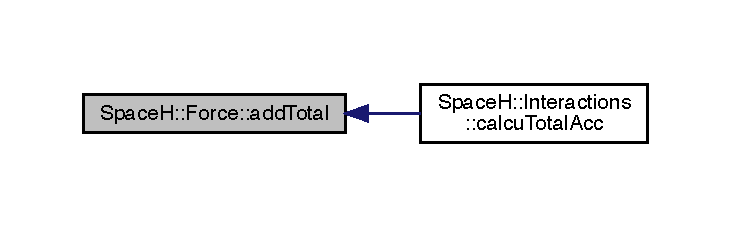
\includegraphics[width=350pt]{struct_space_h_1_1_force_a9f85a2d5e3e642c6e1121c591c19dded_icgraph}
\end{center}
\end{figure}
\mbox{\Hypertarget{struct_space_h_1_1_force_aa1a3ef23a57eb72d0004c4afe505eb0b}\label{struct_space_h_1_1_force_aa1a3ef23a57eb72d0004c4afe505eb0b}} 
\index{Space\+H\+::\+Force@{Space\+H\+::\+Force}!check\+Array\+Size@{check\+Array\+Size}}
\index{check\+Array\+Size@{check\+Array\+Size}!Space\+H\+::\+Force@{Space\+H\+::\+Force}}
\subsubsection{\texorpdfstring{check\+Array\+Size()}{checkArraySize()}}
{\footnotesize\ttfamily template$<$typename Forcefunc, typename Dtype, size\+\_\+t Array\+Size$>$ \\
void \mbox{\hyperlink{struct_space_h_1_1_force}{Space\+H\+::\+Force}}$<$ Forcefunc, Dtype, Array\+Size $>$\+::check\+Array\+Size (\begin{DoxyParamCaption}\item[{size\+\_\+t}]{size }\end{DoxyParamCaption})\hspace{0.3cm}{\ttfamily [inline]}}



\subsection{Member Data Documentation}
\mbox{\Hypertarget{struct_space_h_1_1_force_a9d669e983d78f8bfa0e1a08dd27b6abb}\label{struct_space_h_1_1_force_a9d669e983d78f8bfa0e1a08dd27b6abb}} 
\index{Space\+H\+::\+Force@{Space\+H\+::\+Force}!force\+\_\+@{force\+\_\+}}
\index{force\+\_\+@{force\+\_\+}!Space\+H\+::\+Force@{Space\+H\+::\+Force}}
\subsubsection{\texorpdfstring{force\+\_\+}{force\_}}
{\footnotesize\ttfamily template$<$typename Forcefunc, typename Dtype, size\+\_\+t Array\+Size$>$ \\
Forcefunc \mbox{\hyperlink{struct_space_h_1_1_force}{Space\+H\+::\+Force}}$<$ Forcefunc, Dtype, Array\+Size $>$\+::force\+\_\+\hspace{0.3cm}{\ttfamily [protected]}}

\mbox{\Hypertarget{struct_space_h_1_1_force_a7e87abc40a345bc5e24bdf56ca32f045}\label{struct_space_h_1_1_force_a7e87abc40a345bc5e24bdf56ca32f045}} 
\index{Space\+H\+::\+Force@{Space\+H\+::\+Force}!this\+\_\+acc\+\_\+@{this\+\_\+acc\+\_\+}}
\index{this\+\_\+acc\+\_\+@{this\+\_\+acc\+\_\+}!Space\+H\+::\+Force@{Space\+H\+::\+Force}}
\subsubsection{\texorpdfstring{this\+\_\+acc\+\_\+}{this\_acc\_}}
{\footnotesize\ttfamily template$<$typename Forcefunc, typename Dtype, size\+\_\+t Array\+Size$>$ \\
\mbox{\hyperlink{struct_space_h_1_1_force_aa58fd21903006c1d033713d04b4719f3}{Vector\+Array}} \mbox{\hyperlink{struct_space_h_1_1_force}{Space\+H\+::\+Force}}$<$ Forcefunc, Dtype, Array\+Size $>$\+::this\+\_\+acc\+\_\+\hspace{0.3cm}{\ttfamily [protected]}}



The documentation for this struct was generated from the following file\+:\begin{DoxyCompactItemize}
\item 
interaction/\mbox{\hyperlink{force_8h}{force.\+h}}\end{DoxyCompactItemize}

\hypertarget{struct_space_h_1_1get__value__type}{}\section{SpaceH\+:\+:get\+\_\+value\+\_\+type$<$ T $>$ Struct Template Reference}
\label{struct_space_h_1_1get__value__type}\index{Space\+H\+::get\+\_\+value\+\_\+type$<$ T $>$@{Space\+H\+::get\+\_\+value\+\_\+type$<$ T $>$}}


{\ttfamily \#include $<$dev\+Tools.\+h$>$}

\subsection*{Public Types}
\begin{DoxyCompactItemize}
\item 
using \mbox{\hyperlink{struct_space_h_1_1get__value__type_a22e0b1ebb5f91bb129a9487208ebd7c7}{type}} = decltype(check$<$ T $>$(0))
\end{DoxyCompactItemize}


\subsection{Member Typedef Documentation}
\mbox{\Hypertarget{struct_space_h_1_1get__value__type_a22e0b1ebb5f91bb129a9487208ebd7c7}\label{struct_space_h_1_1get__value__type_a22e0b1ebb5f91bb129a9487208ebd7c7}} 
\index{Space\+H\+::get\+\_\+value\+\_\+type@{Space\+H\+::get\+\_\+value\+\_\+type}!type@{type}}
\index{type@{type}!Space\+H\+::get\+\_\+value\+\_\+type@{Space\+H\+::get\+\_\+value\+\_\+type}}
\subsubsection{\texorpdfstring{type}{type}}
{\footnotesize\ttfamily template$<$typename T$>$ \\
using \mbox{\hyperlink{struct_space_h_1_1get__value__type}{Space\+H\+::get\+\_\+value\+\_\+type}}$<$ T $>$\+::\mbox{\hyperlink{struct_space_h_1_1get__value__type_a22e0b1ebb5f91bb129a9487208ebd7c7}{type}} =  decltype(check$<$T$>$(0))}



The documentation for this struct was generated from the following file\+:\begin{DoxyCompactItemize}
\item 
\mbox{\hyperlink{dev_tools_8h}{dev\+Tools.\+h}}\end{DoxyCompactItemize}

\hypertarget{class_space_h_1_1_interaction}{}\section{SpaceH\+:\+:Interaction$<$ Vel\+Indep, Vel\+Dep, Ext\+Vel\+Indep, Ext\+Vel\+Dep $>$ Class Template Reference}
\label{class_space_h_1_1_interaction}\index{Space\+H\+::\+Interaction$<$ Vel\+Indep, Vel\+Dep, Ext\+Vel\+Indep, Ext\+Vel\+Dep $>$@{Space\+H\+::\+Interaction$<$ Vel\+Indep, Vel\+Dep, Ext\+Vel\+Indep, Ext\+Vel\+Dep $>$}}


{\ttfamily \#include $<$interaction.\+h$>$}

\subsection*{Public Types}
\begin{DoxyCompactItemize}
\item 
using \mbox{\hyperlink{class_space_h_1_1_interaction_a0bed18b8b8efcb42be264a255f931be6}{type}} = typename Vel\+Indep\+::type
\item 
using \mbox{\hyperlink{class_space_h_1_1_interaction_a6ff49274a9233d682fdd75b70ac4d9dc}{Scalar}} = typename type\+::\+Scalar
\item 
using \mbox{\hyperlink{class_space_h_1_1_interaction_ad6d656d30b9272a5f690b0412a4a9a86}{Vector}} = typename type\+::\+Vector
\item 
using \mbox{\hyperlink{class_space_h_1_1_interaction_a9aaccf9a34d875881d9448acf7aaf009}{Vector\+Array}} = typename type\+::\+Vector\+Array
\item 
using \mbox{\hyperlink{class_space_h_1_1_interaction_af9db1e366eeabfcd2dcea3e4343e3f57}{Scalar\+Array}} = typename type\+::\+Scalar\+Array
\end{DoxyCompactItemize}
\subsection*{Public Member Functions}
\begin{DoxyCompactItemize}
\item 
const \mbox{\hyperlink{class_space_h_1_1_interaction_a9aaccf9a34d875881d9448acf7aaf009}{Vector\+Array}} \& \mbox{\hyperlink{class_space_h_1_1_interaction_ae798bbb6d97bc4ff9af4d59a117b2b40}{total\+Acc}} ()
\item 
const \mbox{\hyperlink{class_space_h_1_1_interaction_a9aaccf9a34d875881d9448acf7aaf009}{Vector\+Array}} \& \mbox{\hyperlink{class_space_h_1_1_interaction_a5b5da26af45601a300ec9e0ad7fa2141}{vel\+Indep\+Acc}} ()
\item 
const \mbox{\hyperlink{class_space_h_1_1_interaction_a9aaccf9a34d875881d9448acf7aaf009}{Vector\+Array}} \& \mbox{\hyperlink{class_space_h_1_1_interaction_a87ecd610557033d30958f4eb420b8f88}{vel\+Dep\+Acc}} ()
\item 
const \mbox{\hyperlink{class_space_h_1_1_interaction_a9aaccf9a34d875881d9448acf7aaf009}{Vector\+Array}} \& \mbox{\hyperlink{class_space_h_1_1_interaction_a13f7c7f61c101a863c2dbedb17c31c2e}{ext\+Vel\+Indep\+Acc}} ()
\item 
const \mbox{\hyperlink{class_space_h_1_1_interaction_a9aaccf9a34d875881d9448acf7aaf009}{Vector\+Array}} \& \mbox{\hyperlink{class_space_h_1_1_interaction_a15494ade2b2d4e9c972718bbcf40dd4d}{ext\+Vel\+Dep\+Acc}} ()
\item 
const \mbox{\hyperlink{class_space_h_1_1_interaction_ad6d656d30b9272a5f690b0412a4a9a86}{Vector}} \& \mbox{\hyperlink{class_space_h_1_1_interaction_abb0464f58a3410788de0d3eb4ff76867}{total\+Acc}} (size\+\_\+t i)
\item 
const \mbox{\hyperlink{class_space_h_1_1_interaction_ad6d656d30b9272a5f690b0412a4a9a86}{Vector}} \& \mbox{\hyperlink{class_space_h_1_1_interaction_af2360c5ed9f347420c6ecbe77fc1357d}{vel\+Indep\+Acc}} (size\+\_\+t i)
\item 
const \mbox{\hyperlink{class_space_h_1_1_interaction_ad6d656d30b9272a5f690b0412a4a9a86}{Vector}} \& \mbox{\hyperlink{class_space_h_1_1_interaction_a4f4cf3f4d89514e15bf5f31bdf141a1d}{vel\+Dep\+Acc}} (size\+\_\+t i)
\item 
const \mbox{\hyperlink{class_space_h_1_1_interaction_ad6d656d30b9272a5f690b0412a4a9a86}{Vector}} \& \mbox{\hyperlink{class_space_h_1_1_interaction_aac3afcba9593992baf9311b50265eb6d}{ext\+Vel\+Indep\+Acc}} (size\+\_\+t i)
\item 
const \mbox{\hyperlink{class_space_h_1_1_interaction_ad6d656d30b9272a5f690b0412a4a9a86}{Vector}} \& \mbox{\hyperlink{class_space_h_1_1_interaction_af1b751e13fc15bb66677fcf9459e95a0}{ext\+Vel\+Dep\+Acc}} (size\+\_\+t i)
\item 
{\footnotesize template$<$typename Particles $>$ }\\std\+::enable\+\_\+if$<$ \mbox{\hyperlink{class_vel_indep_particles_a6d357b21c216a2b079b1927c18de0b8f}{Particles\+::data\+Struct}}==\mbox{\hyperlink{namespace_space_h_a0af19f79a6498e99dbda772053d44a72af62eb0bf5e5c72e80983fbbac1cb70e5}{Space\+H\+::\+D\+A\+T\+A\+S\+T\+R\+U\+C\+T\+::\+P\+L\+A\+IN}} $>$\+::\mbox{\hyperlink{class_space_h_1_1_interaction_a0bed18b8b8efcb42be264a255f931be6}{type}} \mbox{\hyperlink{class_space_h_1_1_interaction_a89ebbf351411c3b9526c9890e4ff823c}{calcu\+Vel\+Indep\+Acc}} (const \mbox{\hyperlink{struct_particles}{Particles}} \&partc)
\item 
{\footnotesize template$<$typename Particles $>$ }\\std\+::enable\+\_\+if$<$ \mbox{\hyperlink{class_vel_indep_particles_a6d357b21c216a2b079b1927c18de0b8f}{Particles\+::data\+Struct}}==\mbox{\hyperlink{namespace_space_h_a0af19f79a6498e99dbda772053d44a72a014d2cf3cdc3af6f4f92c09190860e33}{Space\+H\+::\+D\+A\+T\+A\+S\+T\+R\+U\+C\+T\+::\+C\+H\+A\+IN}} $>$\+::\mbox{\hyperlink{class_space_h_1_1_interaction_a0bed18b8b8efcb42be264a255f931be6}{type}} \mbox{\hyperlink{class_space_h_1_1_interaction_a675bfa4741648047ff36592e08a62c32}{calcu\+Vel\+Indep\+Acc}} (const \mbox{\hyperlink{struct_particles}{Particles}} \&partc)
\item 
{\footnotesize template$<$typename Particles $>$ }\\std\+::enable\+\_\+if$<$ \mbox{\hyperlink{class_vel_indep_particles_a6d357b21c216a2b079b1927c18de0b8f}{Particles\+::data\+Struct}}==\mbox{\hyperlink{namespace_space_h_a0af19f79a6498e99dbda772053d44a72af62eb0bf5e5c72e80983fbbac1cb70e5}{Space\+H\+::\+D\+A\+T\+A\+S\+T\+R\+U\+C\+T\+::\+P\+L\+A\+IN}} $>$\+::\mbox{\hyperlink{class_space_h_1_1_interaction_a0bed18b8b8efcb42be264a255f931be6}{type}} \mbox{\hyperlink{class_space_h_1_1_interaction_aa7aa7148a435c420e86821ae319e68b0}{calcu\+Vel\+Dep\+Acc}} (const \mbox{\hyperlink{struct_particles}{Particles}} \&partc)
\item 
{\footnotesize template$<$typename Particles $>$ }\\std\+::enable\+\_\+if$<$ \mbox{\hyperlink{class_vel_indep_particles_a6d357b21c216a2b079b1927c18de0b8f}{Particles\+::data\+Struct}}==\mbox{\hyperlink{namespace_space_h_a0af19f79a6498e99dbda772053d44a72a014d2cf3cdc3af6f4f92c09190860e33}{Space\+H\+::\+D\+A\+T\+A\+S\+T\+R\+U\+C\+T\+::\+C\+H\+A\+IN}} $>$\+::\mbox{\hyperlink{class_space_h_1_1_interaction_a0bed18b8b8efcb42be264a255f931be6}{type}} \mbox{\hyperlink{class_space_h_1_1_interaction_a738430ac153d28064f0068c338cf061f}{calcu\+Vel\+Dep\+Acc}} (const \mbox{\hyperlink{struct_particles}{Particles}} \&partc)
\item 
{\footnotesize template$<$typename Particles $>$ }\\std\+::enable\+\_\+if$<$ \mbox{\hyperlink{class_vel_indep_particles_a6d357b21c216a2b079b1927c18de0b8f}{Particles\+::data\+Struct}}==\mbox{\hyperlink{namespace_space_h_a0af19f79a6498e99dbda772053d44a72af62eb0bf5e5c72e80983fbbac1cb70e5}{Space\+H\+::\+D\+A\+T\+A\+S\+T\+R\+U\+C\+T\+::\+P\+L\+A\+IN}} $>$\+::\mbox{\hyperlink{class_space_h_1_1_interaction_a0bed18b8b8efcb42be264a255f931be6}{type}} \mbox{\hyperlink{class_space_h_1_1_interaction_ae5763f03d500bc392c44d48cf87fe6fb}{calcu\+Auxi\+Vel\+Dep\+Acc}} (const \mbox{\hyperlink{struct_particles}{Particles}} \&partc)
\item 
{\footnotesize template$<$typename Particles $>$ }\\std\+::enable\+\_\+if$<$ \mbox{\hyperlink{class_vel_indep_particles_a6d357b21c216a2b079b1927c18de0b8f}{Particles\+::data\+Struct}}==\mbox{\hyperlink{namespace_space_h_a0af19f79a6498e99dbda772053d44a72a014d2cf3cdc3af6f4f92c09190860e33}{Space\+H\+::\+D\+A\+T\+A\+S\+T\+R\+U\+C\+T\+::\+C\+H\+A\+IN}} $>$\+::\mbox{\hyperlink{class_space_h_1_1_interaction_a0bed18b8b8efcb42be264a255f931be6}{type}} \mbox{\hyperlink{class_space_h_1_1_interaction_addc5bcf2c12d28945af7c78a464b599e}{calcu\+Auxi\+Vel\+Dep\+Acc}} (const \mbox{\hyperlink{struct_particles}{Particles}} \&partc)
\item 
{\footnotesize template$<$typename Particles $>$ }\\void \mbox{\hyperlink{class_space_h_1_1_interaction_a1121ca910c3c919b9239ed57ecb79440}{calcu\+Ext\+Vel\+Indep\+Acc}} (const \mbox{\hyperlink{struct_particles}{Particles}} \&partc)
\item 
{\footnotesize template$<$typename Particles $>$ }\\void \mbox{\hyperlink{class_space_h_1_1_interaction_a171fc6ed61d1e4d842df56d150c5d2ca}{calcu\+Ext\+Vel\+Dep\+Acc}} (const \mbox{\hyperlink{struct_particles}{Particles}} \&partc)
\item 
{\footnotesize template$<$typename Particles $>$ }\\void \mbox{\hyperlink{class_space_h_1_1_interaction_a29ebcdb5fb80bea1f0bc2de302a6cb15}{calcu\+Ext\+Auxi\+Vel\+Dep\+Acc}} (const \mbox{\hyperlink{struct_particles}{Particles}} \&partc)
\item 
void \mbox{\hyperlink{class_space_h_1_1_interaction_a000918130269445ac83b2df6243add07}{zero\+Total\+Acc}} ()
\item 
void \mbox{\hyperlink{class_space_h_1_1_interaction_a28a437fd17fe9b6190ca5aa321264c13}{calcu\+Total\+Acc}} ()
\end{DoxyCompactItemize}
\subsection*{Static Public Attributes}
\begin{DoxyCompactItemize}
\item 
static constexpr bool \mbox{\hyperlink{class_space_h_1_1_interaction_ac2c52753e6cf7f9040d710345caf7635}{is\+Vel\+Dep}} \{ Vel\+Dep\+::is\+Vel\+Dep $\vert$$\vert$ Ext\+Vel\+Dep\+::is\+Vel\+Dep \}
\end{DoxyCompactItemize}


\subsection{Detailed Description}
\subsubsection*{template$<$typename Vel\+Indep, typename Vel\+Dep, typename Ext\+Vel\+Indep, typename Ext\+Vel\+Dep$>$\newline
class Space\+H\+::\+Interaction$<$ Vel\+Indep, Vel\+Dep, Ext\+Vel\+Indep, Ext\+Vel\+Dep $>$}



Definition at line 17 of file interaction.\+h.



\subsection{Member Typedef Documentation}
\mbox{\Hypertarget{class_space_h_1_1_interaction_a6ff49274a9233d682fdd75b70ac4d9dc}\label{class_space_h_1_1_interaction_a6ff49274a9233d682fdd75b70ac4d9dc}} 
\index{Space\+H\+::\+Interaction@{Space\+H\+::\+Interaction}!Scalar@{Scalar}}
\index{Scalar@{Scalar}!Space\+H\+::\+Interaction@{Space\+H\+::\+Interaction}}
\subsubsection{\texorpdfstring{Scalar}{Scalar}}
{\footnotesize\ttfamily template$<$typename Vel\+Indep , typename Vel\+Dep , typename Ext\+Vel\+Indep , typename Ext\+Vel\+Dep $>$ \\
using \mbox{\hyperlink{class_space_h_1_1_interaction}{Space\+H\+::\+Interaction}}$<$ Vel\+Indep, Vel\+Dep, Ext\+Vel\+Indep, Ext\+Vel\+Dep $>$\+::\mbox{\hyperlink{class_space_h_1_1_interaction_a6ff49274a9233d682fdd75b70ac4d9dc}{Scalar}} =  typename type\+::\+Scalar}



Definition at line 22 of file interaction.\+h.

\mbox{\Hypertarget{class_space_h_1_1_interaction_af9db1e366eeabfcd2dcea3e4343e3f57}\label{class_space_h_1_1_interaction_af9db1e366eeabfcd2dcea3e4343e3f57}} 
\index{Space\+H\+::\+Interaction@{Space\+H\+::\+Interaction}!Scalar\+Array@{Scalar\+Array}}
\index{Scalar\+Array@{Scalar\+Array}!Space\+H\+::\+Interaction@{Space\+H\+::\+Interaction}}
\subsubsection{\texorpdfstring{Scalar\+Array}{ScalarArray}}
{\footnotesize\ttfamily template$<$typename Vel\+Indep , typename Vel\+Dep , typename Ext\+Vel\+Indep , typename Ext\+Vel\+Dep $>$ \\
using \mbox{\hyperlink{class_space_h_1_1_interaction}{Space\+H\+::\+Interaction}}$<$ Vel\+Indep, Vel\+Dep, Ext\+Vel\+Indep, Ext\+Vel\+Dep $>$\+::\mbox{\hyperlink{class_space_h_1_1_interaction_af9db1e366eeabfcd2dcea3e4343e3f57}{Scalar\+Array}} =  typename type\+::\+Scalar\+Array}



Definition at line 28 of file interaction.\+h.

\mbox{\Hypertarget{class_space_h_1_1_interaction_a0bed18b8b8efcb42be264a255f931be6}\label{class_space_h_1_1_interaction_a0bed18b8b8efcb42be264a255f931be6}} 
\index{Space\+H\+::\+Interaction@{Space\+H\+::\+Interaction}!type@{type}}
\index{type@{type}!Space\+H\+::\+Interaction@{Space\+H\+::\+Interaction}}
\subsubsection{\texorpdfstring{type}{type}}
{\footnotesize\ttfamily template$<$typename Vel\+Indep , typename Vel\+Dep , typename Ext\+Vel\+Indep , typename Ext\+Vel\+Dep $>$ \\
using \mbox{\hyperlink{class_space_h_1_1_interaction}{Space\+H\+::\+Interaction}}$<$ Vel\+Indep, Vel\+Dep, Ext\+Vel\+Indep, Ext\+Vel\+Dep $>$\+::\mbox{\hyperlink{class_space_h_1_1_interaction_a0bed18b8b8efcb42be264a255f931be6}{type}} =  typename Vel\+Indep\+::type}



Definition at line 20 of file interaction.\+h.

\mbox{\Hypertarget{class_space_h_1_1_interaction_ad6d656d30b9272a5f690b0412a4a9a86}\label{class_space_h_1_1_interaction_ad6d656d30b9272a5f690b0412a4a9a86}} 
\index{Space\+H\+::\+Interaction@{Space\+H\+::\+Interaction}!Vector@{Vector}}
\index{Vector@{Vector}!Space\+H\+::\+Interaction@{Space\+H\+::\+Interaction}}
\subsubsection{\texorpdfstring{Vector}{Vector}}
{\footnotesize\ttfamily template$<$typename Vel\+Indep , typename Vel\+Dep , typename Ext\+Vel\+Indep , typename Ext\+Vel\+Dep $>$ \\
using \mbox{\hyperlink{class_space_h_1_1_interaction}{Space\+H\+::\+Interaction}}$<$ Vel\+Indep, Vel\+Dep, Ext\+Vel\+Indep, Ext\+Vel\+Dep $>$\+::\mbox{\hyperlink{class_space_h_1_1_interaction_ad6d656d30b9272a5f690b0412a4a9a86}{Vector}} =  typename type\+::\+Vector}



Definition at line 24 of file interaction.\+h.

\mbox{\Hypertarget{class_space_h_1_1_interaction_a9aaccf9a34d875881d9448acf7aaf009}\label{class_space_h_1_1_interaction_a9aaccf9a34d875881d9448acf7aaf009}} 
\index{Space\+H\+::\+Interaction@{Space\+H\+::\+Interaction}!Vector\+Array@{Vector\+Array}}
\index{Vector\+Array@{Vector\+Array}!Space\+H\+::\+Interaction@{Space\+H\+::\+Interaction}}
\subsubsection{\texorpdfstring{Vector\+Array}{VectorArray}}
{\footnotesize\ttfamily template$<$typename Vel\+Indep , typename Vel\+Dep , typename Ext\+Vel\+Indep , typename Ext\+Vel\+Dep $>$ \\
using \mbox{\hyperlink{class_space_h_1_1_interaction}{Space\+H\+::\+Interaction}}$<$ Vel\+Indep, Vel\+Dep, Ext\+Vel\+Indep, Ext\+Vel\+Dep $>$\+::\mbox{\hyperlink{class_space_h_1_1_interaction_a9aaccf9a34d875881d9448acf7aaf009}{Vector\+Array}} =  typename type\+::\+Vector\+Array}



Definition at line 26 of file interaction.\+h.



\subsection{Member Function Documentation}
\mbox{\Hypertarget{class_space_h_1_1_interaction_ae5763f03d500bc392c44d48cf87fe6fb}\label{class_space_h_1_1_interaction_ae5763f03d500bc392c44d48cf87fe6fb}} 
\index{Space\+H\+::\+Interaction@{Space\+H\+::\+Interaction}!calcu\+Auxi\+Vel\+Dep\+Acc@{calcu\+Auxi\+Vel\+Dep\+Acc}}
\index{calcu\+Auxi\+Vel\+Dep\+Acc@{calcu\+Auxi\+Vel\+Dep\+Acc}!Space\+H\+::\+Interaction@{Space\+H\+::\+Interaction}}
\subsubsection{\texorpdfstring{calcu\+Auxi\+Vel\+Dep\+Acc()}{calcuAuxiVelDepAcc()}\hspace{0.1cm}{\footnotesize\ttfamily [1/2]}}
{\footnotesize\ttfamily template$<$typename Vel\+Indep , typename Vel\+Dep , typename Ext\+Vel\+Indep , typename Ext\+Vel\+Dep $>$ \\
template$<$typename Particles $>$ \\
std\+::enable\+\_\+if$<$\mbox{\hyperlink{class_vel_indep_particles_a6d357b21c216a2b079b1927c18de0b8f}{Particles\+::data\+Struct}} == \mbox{\hyperlink{namespace_space_h_a0af19f79a6498e99dbda772053d44a72af62eb0bf5e5c72e80983fbbac1cb70e5}{Space\+H\+::\+D\+A\+T\+A\+S\+T\+R\+U\+C\+T\+::\+P\+L\+A\+IN}}$>$\+::\mbox{\hyperlink{class_space_h_1_1_interaction_a0bed18b8b8efcb42be264a255f931be6}{type}} \mbox{\hyperlink{class_space_h_1_1_interaction}{Space\+H\+::\+Interaction}}$<$ Vel\+Indep, Vel\+Dep, Ext\+Vel\+Indep, Ext\+Vel\+Dep $>$\+::calcu\+Auxi\+Vel\+Dep\+Acc (\begin{DoxyParamCaption}\item[{const \mbox{\hyperlink{struct_particles}{Particles}} \&}]{partc }\end{DoxyParamCaption})\hspace{0.3cm}{\ttfamily [inline]}}



Definition at line 84 of file interaction.\+h.

Here is the call graph for this function\+:\nopagebreak
\begin{figure}[H]
\begin{center}
\leavevmode
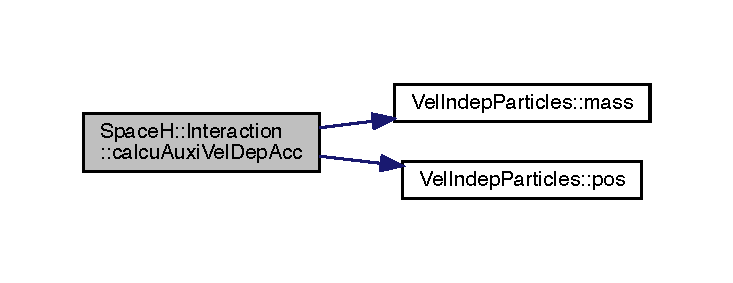
\includegraphics[width=350pt]{class_space_h_1_1_interaction_ae5763f03d500bc392c44d48cf87fe6fb_cgraph}
\end{center}
\end{figure}
\mbox{\Hypertarget{class_space_h_1_1_interaction_addc5bcf2c12d28945af7c78a464b599e}\label{class_space_h_1_1_interaction_addc5bcf2c12d28945af7c78a464b599e}} 
\index{Space\+H\+::\+Interaction@{Space\+H\+::\+Interaction}!calcu\+Auxi\+Vel\+Dep\+Acc@{calcu\+Auxi\+Vel\+Dep\+Acc}}
\index{calcu\+Auxi\+Vel\+Dep\+Acc@{calcu\+Auxi\+Vel\+Dep\+Acc}!Space\+H\+::\+Interaction@{Space\+H\+::\+Interaction}}
\subsubsection{\texorpdfstring{calcu\+Auxi\+Vel\+Dep\+Acc()}{calcuAuxiVelDepAcc()}\hspace{0.1cm}{\footnotesize\ttfamily [2/2]}}
{\footnotesize\ttfamily template$<$typename Vel\+Indep , typename Vel\+Dep , typename Ext\+Vel\+Indep , typename Ext\+Vel\+Dep $>$ \\
template$<$typename Particles $>$ \\
std\+::enable\+\_\+if$<$\mbox{\hyperlink{class_vel_indep_particles_a6d357b21c216a2b079b1927c18de0b8f}{Particles\+::data\+Struct}} == \mbox{\hyperlink{namespace_space_h_a0af19f79a6498e99dbda772053d44a72a014d2cf3cdc3af6f4f92c09190860e33}{Space\+H\+::\+D\+A\+T\+A\+S\+T\+R\+U\+C\+T\+::\+C\+H\+A\+IN}}$>$\+::\mbox{\hyperlink{class_space_h_1_1_interaction_a0bed18b8b8efcb42be264a255f931be6}{type}} \mbox{\hyperlink{class_space_h_1_1_interaction}{Space\+H\+::\+Interaction}}$<$ Vel\+Indep, Vel\+Dep, Ext\+Vel\+Indep, Ext\+Vel\+Dep $>$\+::calcu\+Auxi\+Vel\+Dep\+Acc (\begin{DoxyParamCaption}\item[{const \mbox{\hyperlink{struct_particles}{Particles}} \&}]{partc }\end{DoxyParamCaption})\hspace{0.3cm}{\ttfamily [inline]}}



Definition at line 91 of file interaction.\+h.

Here is the call graph for this function\+:\nopagebreak
\begin{figure}[H]
\begin{center}
\leavevmode
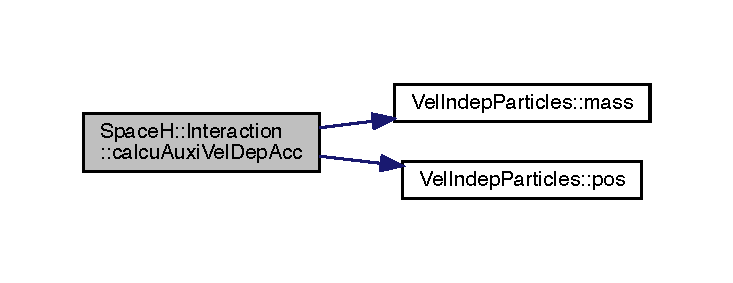
\includegraphics[width=350pt]{class_space_h_1_1_interaction_addc5bcf2c12d28945af7c78a464b599e_cgraph}
\end{center}
\end{figure}
\mbox{\Hypertarget{class_space_h_1_1_interaction_a29ebcdb5fb80bea1f0bc2de302a6cb15}\label{class_space_h_1_1_interaction_a29ebcdb5fb80bea1f0bc2de302a6cb15}} 
\index{Space\+H\+::\+Interaction@{Space\+H\+::\+Interaction}!calcu\+Ext\+Auxi\+Vel\+Dep\+Acc@{calcu\+Ext\+Auxi\+Vel\+Dep\+Acc}}
\index{calcu\+Ext\+Auxi\+Vel\+Dep\+Acc@{calcu\+Ext\+Auxi\+Vel\+Dep\+Acc}!Space\+H\+::\+Interaction@{Space\+H\+::\+Interaction}}
\subsubsection{\texorpdfstring{calcu\+Ext\+Auxi\+Vel\+Dep\+Acc()}{calcuExtAuxiVelDepAcc()}}
{\footnotesize\ttfamily template$<$typename Vel\+Indep , typename Vel\+Dep , typename Ext\+Vel\+Indep , typename Ext\+Vel\+Dep $>$ \\
template$<$typename Particles $>$ \\
void \mbox{\hyperlink{class_space_h_1_1_interaction}{Space\+H\+::\+Interaction}}$<$ Vel\+Indep, Vel\+Dep, Ext\+Vel\+Indep, Ext\+Vel\+Dep $>$\+::calcu\+Ext\+Auxi\+Vel\+Dep\+Acc (\begin{DoxyParamCaption}\item[{const \mbox{\hyperlink{struct_particles}{Particles}} \&}]{partc }\end{DoxyParamCaption})\hspace{0.3cm}{\ttfamily [inline]}}



Definition at line 109 of file interaction.\+h.

Here is the call graph for this function\+:\nopagebreak
\begin{figure}[H]
\begin{center}
\leavevmode
\includegraphics[width=350pt]{class_space_h_1_1_interaction_a29ebcdb5fb80bea1f0bc2de302a6cb15_cgraph}
\end{center}
\end{figure}
\mbox{\Hypertarget{class_space_h_1_1_interaction_a171fc6ed61d1e4d842df56d150c5d2ca}\label{class_space_h_1_1_interaction_a171fc6ed61d1e4d842df56d150c5d2ca}} 
\index{Space\+H\+::\+Interaction@{Space\+H\+::\+Interaction}!calcu\+Ext\+Vel\+Dep\+Acc@{calcu\+Ext\+Vel\+Dep\+Acc}}
\index{calcu\+Ext\+Vel\+Dep\+Acc@{calcu\+Ext\+Vel\+Dep\+Acc}!Space\+H\+::\+Interaction@{Space\+H\+::\+Interaction}}
\subsubsection{\texorpdfstring{calcu\+Ext\+Vel\+Dep\+Acc()}{calcuExtVelDepAcc()}}
{\footnotesize\ttfamily template$<$typename Vel\+Indep , typename Vel\+Dep , typename Ext\+Vel\+Indep , typename Ext\+Vel\+Dep $>$ \\
template$<$typename Particles $>$ \\
void \mbox{\hyperlink{class_space_h_1_1_interaction}{Space\+H\+::\+Interaction}}$<$ Vel\+Indep, Vel\+Dep, Ext\+Vel\+Indep, Ext\+Vel\+Dep $>$\+::calcu\+Ext\+Vel\+Dep\+Acc (\begin{DoxyParamCaption}\item[{const \mbox{\hyperlink{struct_particles}{Particles}} \&}]{partc }\end{DoxyParamCaption})\hspace{0.3cm}{\ttfamily [inline]}}



Definition at line 103 of file interaction.\+h.

Here is the call graph for this function\+:\nopagebreak
\begin{figure}[H]
\begin{center}
\leavevmode
\includegraphics[width=347pt]{class_space_h_1_1_interaction_a171fc6ed61d1e4d842df56d150c5d2ca_cgraph}
\end{center}
\end{figure}
\mbox{\Hypertarget{class_space_h_1_1_interaction_a1121ca910c3c919b9239ed57ecb79440}\label{class_space_h_1_1_interaction_a1121ca910c3c919b9239ed57ecb79440}} 
\index{Space\+H\+::\+Interaction@{Space\+H\+::\+Interaction}!calcu\+Ext\+Vel\+Indep\+Acc@{calcu\+Ext\+Vel\+Indep\+Acc}}
\index{calcu\+Ext\+Vel\+Indep\+Acc@{calcu\+Ext\+Vel\+Indep\+Acc}!Space\+H\+::\+Interaction@{Space\+H\+::\+Interaction}}
\subsubsection{\texorpdfstring{calcu\+Ext\+Vel\+Indep\+Acc()}{calcuExtVelIndepAcc()}}
{\footnotesize\ttfamily template$<$typename Vel\+Indep , typename Vel\+Dep , typename Ext\+Vel\+Indep , typename Ext\+Vel\+Dep $>$ \\
template$<$typename Particles $>$ \\
void \mbox{\hyperlink{class_space_h_1_1_interaction}{Space\+H\+::\+Interaction}}$<$ Vel\+Indep, Vel\+Dep, Ext\+Vel\+Indep, Ext\+Vel\+Dep $>$\+::calcu\+Ext\+Vel\+Indep\+Acc (\begin{DoxyParamCaption}\item[{const \mbox{\hyperlink{struct_particles}{Particles}} \&}]{partc }\end{DoxyParamCaption})\hspace{0.3cm}{\ttfamily [inline]}}



Definition at line 97 of file interaction.\+h.

Here is the call graph for this function\+:\nopagebreak
\begin{figure}[H]
\begin{center}
\leavevmode
\includegraphics[width=350pt]{class_space_h_1_1_interaction_a1121ca910c3c919b9239ed57ecb79440_cgraph}
\end{center}
\end{figure}
\mbox{\Hypertarget{class_space_h_1_1_interaction_a28a437fd17fe9b6190ca5aa321264c13}\label{class_space_h_1_1_interaction_a28a437fd17fe9b6190ca5aa321264c13}} 
\index{Space\+H\+::\+Interaction@{Space\+H\+::\+Interaction}!calcu\+Total\+Acc@{calcu\+Total\+Acc}}
\index{calcu\+Total\+Acc@{calcu\+Total\+Acc}!Space\+H\+::\+Interaction@{Space\+H\+::\+Interaction}}
\subsubsection{\texorpdfstring{calcu\+Total\+Acc()}{calcuTotalAcc()}}
{\footnotesize\ttfamily template$<$typename Vel\+Indep , typename Vel\+Dep , typename Ext\+Vel\+Indep , typename Ext\+Vel\+Dep $>$ \\
void \mbox{\hyperlink{class_space_h_1_1_interaction}{Space\+H\+::\+Interaction}}$<$ Vel\+Indep, Vel\+Dep, Ext\+Vel\+Indep, Ext\+Vel\+Dep $>$\+::calcu\+Total\+Acc (\begin{DoxyParamCaption}{ }\end{DoxyParamCaption})\hspace{0.3cm}{\ttfamily [inline]}}



Definition at line 121 of file interaction.\+h.

\mbox{\Hypertarget{class_space_h_1_1_interaction_aa7aa7148a435c420e86821ae319e68b0}\label{class_space_h_1_1_interaction_aa7aa7148a435c420e86821ae319e68b0}} 
\index{Space\+H\+::\+Interaction@{Space\+H\+::\+Interaction}!calcu\+Vel\+Dep\+Acc@{calcu\+Vel\+Dep\+Acc}}
\index{calcu\+Vel\+Dep\+Acc@{calcu\+Vel\+Dep\+Acc}!Space\+H\+::\+Interaction@{Space\+H\+::\+Interaction}}
\subsubsection{\texorpdfstring{calcu\+Vel\+Dep\+Acc()}{calcuVelDepAcc()}\hspace{0.1cm}{\footnotesize\ttfamily [1/2]}}
{\footnotesize\ttfamily template$<$typename Vel\+Indep , typename Vel\+Dep , typename Ext\+Vel\+Indep , typename Ext\+Vel\+Dep $>$ \\
template$<$typename Particles $>$ \\
std\+::enable\+\_\+if$<$\mbox{\hyperlink{class_vel_indep_particles_a6d357b21c216a2b079b1927c18de0b8f}{Particles\+::data\+Struct}} == \mbox{\hyperlink{namespace_space_h_a0af19f79a6498e99dbda772053d44a72af62eb0bf5e5c72e80983fbbac1cb70e5}{Space\+H\+::\+D\+A\+T\+A\+S\+T\+R\+U\+C\+T\+::\+P\+L\+A\+IN}}$>$\+::\mbox{\hyperlink{class_space_h_1_1_interaction_a0bed18b8b8efcb42be264a255f931be6}{type}} \mbox{\hyperlink{class_space_h_1_1_interaction}{Space\+H\+::\+Interaction}}$<$ Vel\+Indep, Vel\+Dep, Ext\+Vel\+Indep, Ext\+Vel\+Dep $>$\+::calcu\+Vel\+Dep\+Acc (\begin{DoxyParamCaption}\item[{const \mbox{\hyperlink{struct_particles}{Particles}} \&}]{partc }\end{DoxyParamCaption})\hspace{0.3cm}{\ttfamily [inline]}}



Definition at line 70 of file interaction.\+h.

Here is the call graph for this function\+:\nopagebreak
\begin{figure}[H]
\begin{center}
\leavevmode
\includegraphics[width=343pt]{class_space_h_1_1_interaction_aa7aa7148a435c420e86821ae319e68b0_cgraph}
\end{center}
\end{figure}
\mbox{\Hypertarget{class_space_h_1_1_interaction_a738430ac153d28064f0068c338cf061f}\label{class_space_h_1_1_interaction_a738430ac153d28064f0068c338cf061f}} 
\index{Space\+H\+::\+Interaction@{Space\+H\+::\+Interaction}!calcu\+Vel\+Dep\+Acc@{calcu\+Vel\+Dep\+Acc}}
\index{calcu\+Vel\+Dep\+Acc@{calcu\+Vel\+Dep\+Acc}!Space\+H\+::\+Interaction@{Space\+H\+::\+Interaction}}
\subsubsection{\texorpdfstring{calcu\+Vel\+Dep\+Acc()}{calcuVelDepAcc()}\hspace{0.1cm}{\footnotesize\ttfamily [2/2]}}
{\footnotesize\ttfamily template$<$typename Vel\+Indep , typename Vel\+Dep , typename Ext\+Vel\+Indep , typename Ext\+Vel\+Dep $>$ \\
template$<$typename Particles $>$ \\
std\+::enable\+\_\+if$<$\mbox{\hyperlink{class_vel_indep_particles_a6d357b21c216a2b079b1927c18de0b8f}{Particles\+::data\+Struct}} == \mbox{\hyperlink{namespace_space_h_a0af19f79a6498e99dbda772053d44a72a014d2cf3cdc3af6f4f92c09190860e33}{Space\+H\+::\+D\+A\+T\+A\+S\+T\+R\+U\+C\+T\+::\+C\+H\+A\+IN}}$>$\+::\mbox{\hyperlink{class_space_h_1_1_interaction_a0bed18b8b8efcb42be264a255f931be6}{type}} \mbox{\hyperlink{class_space_h_1_1_interaction}{Space\+H\+::\+Interaction}}$<$ Vel\+Indep, Vel\+Dep, Ext\+Vel\+Indep, Ext\+Vel\+Dep $>$\+::calcu\+Vel\+Dep\+Acc (\begin{DoxyParamCaption}\item[{const \mbox{\hyperlink{struct_particles}{Particles}} \&}]{partc }\end{DoxyParamCaption})\hspace{0.3cm}{\ttfamily [inline]}}



Definition at line 77 of file interaction.\+h.

Here is the call graph for this function\+:\nopagebreak
\begin{figure}[H]
\begin{center}
\leavevmode
\includegraphics[width=343pt]{class_space_h_1_1_interaction_a738430ac153d28064f0068c338cf061f_cgraph}
\end{center}
\end{figure}
\mbox{\Hypertarget{class_space_h_1_1_interaction_a89ebbf351411c3b9526c9890e4ff823c}\label{class_space_h_1_1_interaction_a89ebbf351411c3b9526c9890e4ff823c}} 
\index{Space\+H\+::\+Interaction@{Space\+H\+::\+Interaction}!calcu\+Vel\+Indep\+Acc@{calcu\+Vel\+Indep\+Acc}}
\index{calcu\+Vel\+Indep\+Acc@{calcu\+Vel\+Indep\+Acc}!Space\+H\+::\+Interaction@{Space\+H\+::\+Interaction}}
\subsubsection{\texorpdfstring{calcu\+Vel\+Indep\+Acc()}{calcuVelIndepAcc()}\hspace{0.1cm}{\footnotesize\ttfamily [1/2]}}
{\footnotesize\ttfamily template$<$typename Vel\+Indep , typename Vel\+Dep , typename Ext\+Vel\+Indep , typename Ext\+Vel\+Dep $>$ \\
template$<$typename Particles $>$ \\
std\+::enable\+\_\+if$<$\mbox{\hyperlink{class_vel_indep_particles_a6d357b21c216a2b079b1927c18de0b8f}{Particles\+::data\+Struct}} == \mbox{\hyperlink{namespace_space_h_a0af19f79a6498e99dbda772053d44a72af62eb0bf5e5c72e80983fbbac1cb70e5}{Space\+H\+::\+D\+A\+T\+A\+S\+T\+R\+U\+C\+T\+::\+P\+L\+A\+IN}}$>$\+::\mbox{\hyperlink{class_space_h_1_1_interaction_a0bed18b8b8efcb42be264a255f931be6}{type}} \mbox{\hyperlink{class_space_h_1_1_interaction}{Space\+H\+::\+Interaction}}$<$ Vel\+Indep, Vel\+Dep, Ext\+Vel\+Indep, Ext\+Vel\+Dep $>$\+::calcu\+Vel\+Indep\+Acc (\begin{DoxyParamCaption}\item[{const \mbox{\hyperlink{struct_particles}{Particles}} \&}]{partc }\end{DoxyParamCaption})\hspace{0.3cm}{\ttfamily [inline]}}



Definition at line 56 of file interaction.\+h.

Here is the call graph for this function\+:\nopagebreak
\begin{figure}[H]
\begin{center}
\leavevmode
\includegraphics[width=343pt]{class_space_h_1_1_interaction_a89ebbf351411c3b9526c9890e4ff823c_cgraph}
\end{center}
\end{figure}
\mbox{\Hypertarget{class_space_h_1_1_interaction_a675bfa4741648047ff36592e08a62c32}\label{class_space_h_1_1_interaction_a675bfa4741648047ff36592e08a62c32}} 
\index{Space\+H\+::\+Interaction@{Space\+H\+::\+Interaction}!calcu\+Vel\+Indep\+Acc@{calcu\+Vel\+Indep\+Acc}}
\index{calcu\+Vel\+Indep\+Acc@{calcu\+Vel\+Indep\+Acc}!Space\+H\+::\+Interaction@{Space\+H\+::\+Interaction}}
\subsubsection{\texorpdfstring{calcu\+Vel\+Indep\+Acc()}{calcuVelIndepAcc()}\hspace{0.1cm}{\footnotesize\ttfamily [2/2]}}
{\footnotesize\ttfamily template$<$typename Vel\+Indep , typename Vel\+Dep , typename Ext\+Vel\+Indep , typename Ext\+Vel\+Dep $>$ \\
template$<$typename Particles $>$ \\
std\+::enable\+\_\+if$<$\mbox{\hyperlink{class_vel_indep_particles_a6d357b21c216a2b079b1927c18de0b8f}{Particles\+::data\+Struct}} == \mbox{\hyperlink{namespace_space_h_a0af19f79a6498e99dbda772053d44a72a014d2cf3cdc3af6f4f92c09190860e33}{Space\+H\+::\+D\+A\+T\+A\+S\+T\+R\+U\+C\+T\+::\+C\+H\+A\+IN}}$>$\+::\mbox{\hyperlink{class_space_h_1_1_interaction_a0bed18b8b8efcb42be264a255f931be6}{type}} \mbox{\hyperlink{class_space_h_1_1_interaction}{Space\+H\+::\+Interaction}}$<$ Vel\+Indep, Vel\+Dep, Ext\+Vel\+Indep, Ext\+Vel\+Dep $>$\+::calcu\+Vel\+Indep\+Acc (\begin{DoxyParamCaption}\item[{const \mbox{\hyperlink{struct_particles}{Particles}} \&}]{partc }\end{DoxyParamCaption})\hspace{0.3cm}{\ttfamily [inline]}}



Definition at line 63 of file interaction.\+h.

Here is the call graph for this function\+:\nopagebreak
\begin{figure}[H]
\begin{center}
\leavevmode
\includegraphics[width=343pt]{class_space_h_1_1_interaction_a675bfa4741648047ff36592e08a62c32_cgraph}
\end{center}
\end{figure}
\mbox{\Hypertarget{class_space_h_1_1_interaction_a15494ade2b2d4e9c972718bbcf40dd4d}\label{class_space_h_1_1_interaction_a15494ade2b2d4e9c972718bbcf40dd4d}} 
\index{Space\+H\+::\+Interaction@{Space\+H\+::\+Interaction}!ext\+Vel\+Dep\+Acc@{ext\+Vel\+Dep\+Acc}}
\index{ext\+Vel\+Dep\+Acc@{ext\+Vel\+Dep\+Acc}!Space\+H\+::\+Interaction@{Space\+H\+::\+Interaction}}
\subsubsection{\texorpdfstring{ext\+Vel\+Dep\+Acc()}{extVelDepAcc()}\hspace{0.1cm}{\footnotesize\ttfamily [1/2]}}
{\footnotesize\ttfamily template$<$typename Vel\+Indep , typename Vel\+Dep , typename Ext\+Vel\+Indep , typename Ext\+Vel\+Dep $>$ \\
const \mbox{\hyperlink{class_space_h_1_1_interaction_a9aaccf9a34d875881d9448acf7aaf009}{Vector\+Array}}\& \mbox{\hyperlink{class_space_h_1_1_interaction}{Space\+H\+::\+Interaction}}$<$ Vel\+Indep, Vel\+Dep, Ext\+Vel\+Indep, Ext\+Vel\+Dep $>$\+::ext\+Vel\+Dep\+Acc (\begin{DoxyParamCaption}{ }\end{DoxyParamCaption})\hspace{0.3cm}{\ttfamily [inline]}}



Definition at line 41 of file interaction.\+h.

\mbox{\Hypertarget{class_space_h_1_1_interaction_af1b751e13fc15bb66677fcf9459e95a0}\label{class_space_h_1_1_interaction_af1b751e13fc15bb66677fcf9459e95a0}} 
\index{Space\+H\+::\+Interaction@{Space\+H\+::\+Interaction}!ext\+Vel\+Dep\+Acc@{ext\+Vel\+Dep\+Acc}}
\index{ext\+Vel\+Dep\+Acc@{ext\+Vel\+Dep\+Acc}!Space\+H\+::\+Interaction@{Space\+H\+::\+Interaction}}
\subsubsection{\texorpdfstring{ext\+Vel\+Dep\+Acc()}{extVelDepAcc()}\hspace{0.1cm}{\footnotesize\ttfamily [2/2]}}
{\footnotesize\ttfamily template$<$typename Vel\+Indep , typename Vel\+Dep , typename Ext\+Vel\+Indep , typename Ext\+Vel\+Dep $>$ \\
const \mbox{\hyperlink{class_space_h_1_1_interaction_ad6d656d30b9272a5f690b0412a4a9a86}{Vector}}\& \mbox{\hyperlink{class_space_h_1_1_interaction}{Space\+H\+::\+Interaction}}$<$ Vel\+Indep, Vel\+Dep, Ext\+Vel\+Indep, Ext\+Vel\+Dep $>$\+::ext\+Vel\+Dep\+Acc (\begin{DoxyParamCaption}\item[{size\+\_\+t}]{i }\end{DoxyParamCaption})\hspace{0.3cm}{\ttfamily [inline]}}



Definition at line 51 of file interaction.\+h.

\mbox{\Hypertarget{class_space_h_1_1_interaction_a13f7c7f61c101a863c2dbedb17c31c2e}\label{class_space_h_1_1_interaction_a13f7c7f61c101a863c2dbedb17c31c2e}} 
\index{Space\+H\+::\+Interaction@{Space\+H\+::\+Interaction}!ext\+Vel\+Indep\+Acc@{ext\+Vel\+Indep\+Acc}}
\index{ext\+Vel\+Indep\+Acc@{ext\+Vel\+Indep\+Acc}!Space\+H\+::\+Interaction@{Space\+H\+::\+Interaction}}
\subsubsection{\texorpdfstring{ext\+Vel\+Indep\+Acc()}{extVelIndepAcc()}\hspace{0.1cm}{\footnotesize\ttfamily [1/2]}}
{\footnotesize\ttfamily template$<$typename Vel\+Indep , typename Vel\+Dep , typename Ext\+Vel\+Indep , typename Ext\+Vel\+Dep $>$ \\
const \mbox{\hyperlink{class_space_h_1_1_interaction_a9aaccf9a34d875881d9448acf7aaf009}{Vector\+Array}}\& \mbox{\hyperlink{class_space_h_1_1_interaction}{Space\+H\+::\+Interaction}}$<$ Vel\+Indep, Vel\+Dep, Ext\+Vel\+Indep, Ext\+Vel\+Dep $>$\+::ext\+Vel\+Indep\+Acc (\begin{DoxyParamCaption}{ }\end{DoxyParamCaption})\hspace{0.3cm}{\ttfamily [inline]}}



Definition at line 39 of file interaction.\+h.

\mbox{\Hypertarget{class_space_h_1_1_interaction_aac3afcba9593992baf9311b50265eb6d}\label{class_space_h_1_1_interaction_aac3afcba9593992baf9311b50265eb6d}} 
\index{Space\+H\+::\+Interaction@{Space\+H\+::\+Interaction}!ext\+Vel\+Indep\+Acc@{ext\+Vel\+Indep\+Acc}}
\index{ext\+Vel\+Indep\+Acc@{ext\+Vel\+Indep\+Acc}!Space\+H\+::\+Interaction@{Space\+H\+::\+Interaction}}
\subsubsection{\texorpdfstring{ext\+Vel\+Indep\+Acc()}{extVelIndepAcc()}\hspace{0.1cm}{\footnotesize\ttfamily [2/2]}}
{\footnotesize\ttfamily template$<$typename Vel\+Indep , typename Vel\+Dep , typename Ext\+Vel\+Indep , typename Ext\+Vel\+Dep $>$ \\
const \mbox{\hyperlink{class_space_h_1_1_interaction_ad6d656d30b9272a5f690b0412a4a9a86}{Vector}}\& \mbox{\hyperlink{class_space_h_1_1_interaction}{Space\+H\+::\+Interaction}}$<$ Vel\+Indep, Vel\+Dep, Ext\+Vel\+Indep, Ext\+Vel\+Dep $>$\+::ext\+Vel\+Indep\+Acc (\begin{DoxyParamCaption}\item[{size\+\_\+t}]{i }\end{DoxyParamCaption})\hspace{0.3cm}{\ttfamily [inline]}}



Definition at line 49 of file interaction.\+h.

\mbox{\Hypertarget{class_space_h_1_1_interaction_ae798bbb6d97bc4ff9af4d59a117b2b40}\label{class_space_h_1_1_interaction_ae798bbb6d97bc4ff9af4d59a117b2b40}} 
\index{Space\+H\+::\+Interaction@{Space\+H\+::\+Interaction}!total\+Acc@{total\+Acc}}
\index{total\+Acc@{total\+Acc}!Space\+H\+::\+Interaction@{Space\+H\+::\+Interaction}}
\subsubsection{\texorpdfstring{total\+Acc()}{totalAcc()}\hspace{0.1cm}{\footnotesize\ttfamily [1/2]}}
{\footnotesize\ttfamily template$<$typename Vel\+Indep , typename Vel\+Dep , typename Ext\+Vel\+Indep , typename Ext\+Vel\+Dep $>$ \\
const \mbox{\hyperlink{class_space_h_1_1_interaction_a9aaccf9a34d875881d9448acf7aaf009}{Vector\+Array}}\& \mbox{\hyperlink{class_space_h_1_1_interaction}{Space\+H\+::\+Interaction}}$<$ Vel\+Indep, Vel\+Dep, Ext\+Vel\+Indep, Ext\+Vel\+Dep $>$\+::total\+Acc (\begin{DoxyParamCaption}{ }\end{DoxyParamCaption})\hspace{0.3cm}{\ttfamily [inline]}}



Definition at line 33 of file interaction.\+h.

\mbox{\Hypertarget{class_space_h_1_1_interaction_abb0464f58a3410788de0d3eb4ff76867}\label{class_space_h_1_1_interaction_abb0464f58a3410788de0d3eb4ff76867}} 
\index{Space\+H\+::\+Interaction@{Space\+H\+::\+Interaction}!total\+Acc@{total\+Acc}}
\index{total\+Acc@{total\+Acc}!Space\+H\+::\+Interaction@{Space\+H\+::\+Interaction}}
\subsubsection{\texorpdfstring{total\+Acc()}{totalAcc()}\hspace{0.1cm}{\footnotesize\ttfamily [2/2]}}
{\footnotesize\ttfamily template$<$typename Vel\+Indep , typename Vel\+Dep , typename Ext\+Vel\+Indep , typename Ext\+Vel\+Dep $>$ \\
const \mbox{\hyperlink{class_space_h_1_1_interaction_ad6d656d30b9272a5f690b0412a4a9a86}{Vector}}\& \mbox{\hyperlink{class_space_h_1_1_interaction}{Space\+H\+::\+Interaction}}$<$ Vel\+Indep, Vel\+Dep, Ext\+Vel\+Indep, Ext\+Vel\+Dep $>$\+::total\+Acc (\begin{DoxyParamCaption}\item[{size\+\_\+t}]{i }\end{DoxyParamCaption})\hspace{0.3cm}{\ttfamily [inline]}}



Definition at line 43 of file interaction.\+h.

\mbox{\Hypertarget{class_space_h_1_1_interaction_a87ecd610557033d30958f4eb420b8f88}\label{class_space_h_1_1_interaction_a87ecd610557033d30958f4eb420b8f88}} 
\index{Space\+H\+::\+Interaction@{Space\+H\+::\+Interaction}!vel\+Dep\+Acc@{vel\+Dep\+Acc}}
\index{vel\+Dep\+Acc@{vel\+Dep\+Acc}!Space\+H\+::\+Interaction@{Space\+H\+::\+Interaction}}
\subsubsection{\texorpdfstring{vel\+Dep\+Acc()}{velDepAcc()}\hspace{0.1cm}{\footnotesize\ttfamily [1/2]}}
{\footnotesize\ttfamily template$<$typename Vel\+Indep , typename Vel\+Dep , typename Ext\+Vel\+Indep , typename Ext\+Vel\+Dep $>$ \\
const \mbox{\hyperlink{class_space_h_1_1_interaction_a9aaccf9a34d875881d9448acf7aaf009}{Vector\+Array}}\& \mbox{\hyperlink{class_space_h_1_1_interaction}{Space\+H\+::\+Interaction}}$<$ Vel\+Indep, Vel\+Dep, Ext\+Vel\+Indep, Ext\+Vel\+Dep $>$\+::vel\+Dep\+Acc (\begin{DoxyParamCaption}{ }\end{DoxyParamCaption})\hspace{0.3cm}{\ttfamily [inline]}}



Definition at line 37 of file interaction.\+h.

\mbox{\Hypertarget{class_space_h_1_1_interaction_a4f4cf3f4d89514e15bf5f31bdf141a1d}\label{class_space_h_1_1_interaction_a4f4cf3f4d89514e15bf5f31bdf141a1d}} 
\index{Space\+H\+::\+Interaction@{Space\+H\+::\+Interaction}!vel\+Dep\+Acc@{vel\+Dep\+Acc}}
\index{vel\+Dep\+Acc@{vel\+Dep\+Acc}!Space\+H\+::\+Interaction@{Space\+H\+::\+Interaction}}
\subsubsection{\texorpdfstring{vel\+Dep\+Acc()}{velDepAcc()}\hspace{0.1cm}{\footnotesize\ttfamily [2/2]}}
{\footnotesize\ttfamily template$<$typename Vel\+Indep , typename Vel\+Dep , typename Ext\+Vel\+Indep , typename Ext\+Vel\+Dep $>$ \\
const \mbox{\hyperlink{class_space_h_1_1_interaction_ad6d656d30b9272a5f690b0412a4a9a86}{Vector}}\& \mbox{\hyperlink{class_space_h_1_1_interaction}{Space\+H\+::\+Interaction}}$<$ Vel\+Indep, Vel\+Dep, Ext\+Vel\+Indep, Ext\+Vel\+Dep $>$\+::vel\+Dep\+Acc (\begin{DoxyParamCaption}\item[{size\+\_\+t}]{i }\end{DoxyParamCaption})\hspace{0.3cm}{\ttfamily [inline]}}



Definition at line 47 of file interaction.\+h.

\mbox{\Hypertarget{class_space_h_1_1_interaction_a5b5da26af45601a300ec9e0ad7fa2141}\label{class_space_h_1_1_interaction_a5b5da26af45601a300ec9e0ad7fa2141}} 
\index{Space\+H\+::\+Interaction@{Space\+H\+::\+Interaction}!vel\+Indep\+Acc@{vel\+Indep\+Acc}}
\index{vel\+Indep\+Acc@{vel\+Indep\+Acc}!Space\+H\+::\+Interaction@{Space\+H\+::\+Interaction}}
\subsubsection{\texorpdfstring{vel\+Indep\+Acc()}{velIndepAcc()}\hspace{0.1cm}{\footnotesize\ttfamily [1/2]}}
{\footnotesize\ttfamily template$<$typename Vel\+Indep , typename Vel\+Dep , typename Ext\+Vel\+Indep , typename Ext\+Vel\+Dep $>$ \\
const \mbox{\hyperlink{class_space_h_1_1_interaction_a9aaccf9a34d875881d9448acf7aaf009}{Vector\+Array}}\& \mbox{\hyperlink{class_space_h_1_1_interaction}{Space\+H\+::\+Interaction}}$<$ Vel\+Indep, Vel\+Dep, Ext\+Vel\+Indep, Ext\+Vel\+Dep $>$\+::vel\+Indep\+Acc (\begin{DoxyParamCaption}{ }\end{DoxyParamCaption})\hspace{0.3cm}{\ttfamily [inline]}}



Definition at line 35 of file interaction.\+h.

\mbox{\Hypertarget{class_space_h_1_1_interaction_af2360c5ed9f347420c6ecbe77fc1357d}\label{class_space_h_1_1_interaction_af2360c5ed9f347420c6ecbe77fc1357d}} 
\index{Space\+H\+::\+Interaction@{Space\+H\+::\+Interaction}!vel\+Indep\+Acc@{vel\+Indep\+Acc}}
\index{vel\+Indep\+Acc@{vel\+Indep\+Acc}!Space\+H\+::\+Interaction@{Space\+H\+::\+Interaction}}
\subsubsection{\texorpdfstring{vel\+Indep\+Acc()}{velIndepAcc()}\hspace{0.1cm}{\footnotesize\ttfamily [2/2]}}
{\footnotesize\ttfamily template$<$typename Vel\+Indep , typename Vel\+Dep , typename Ext\+Vel\+Indep , typename Ext\+Vel\+Dep $>$ \\
const \mbox{\hyperlink{class_space_h_1_1_interaction_ad6d656d30b9272a5f690b0412a4a9a86}{Vector}}\& \mbox{\hyperlink{class_space_h_1_1_interaction}{Space\+H\+::\+Interaction}}$<$ Vel\+Indep, Vel\+Dep, Ext\+Vel\+Indep, Ext\+Vel\+Dep $>$\+::vel\+Indep\+Acc (\begin{DoxyParamCaption}\item[{size\+\_\+t}]{i }\end{DoxyParamCaption})\hspace{0.3cm}{\ttfamily [inline]}}



Definition at line 45 of file interaction.\+h.

\mbox{\Hypertarget{class_space_h_1_1_interaction_a000918130269445ac83b2df6243add07}\label{class_space_h_1_1_interaction_a000918130269445ac83b2df6243add07}} 
\index{Space\+H\+::\+Interaction@{Space\+H\+::\+Interaction}!zero\+Total\+Acc@{zero\+Total\+Acc}}
\index{zero\+Total\+Acc@{zero\+Total\+Acc}!Space\+H\+::\+Interaction@{Space\+H\+::\+Interaction}}
\subsubsection{\texorpdfstring{zero\+Total\+Acc()}{zeroTotalAcc()}}
{\footnotesize\ttfamily template$<$typename Vel\+Indep , typename Vel\+Dep , typename Ext\+Vel\+Indep , typename Ext\+Vel\+Dep $>$ \\
void \mbox{\hyperlink{class_space_h_1_1_interaction}{Space\+H\+::\+Interaction}}$<$ Vel\+Indep, Vel\+Dep, Ext\+Vel\+Indep, Ext\+Vel\+Dep $>$\+::zero\+Total\+Acc (\begin{DoxyParamCaption}{ }\end{DoxyParamCaption})\hspace{0.3cm}{\ttfamily [inline]}}



Definition at line 114 of file interaction.\+h.



\subsection{Member Data Documentation}
\mbox{\Hypertarget{class_space_h_1_1_interaction_ac2c52753e6cf7f9040d710345caf7635}\label{class_space_h_1_1_interaction_ac2c52753e6cf7f9040d710345caf7635}} 
\index{Space\+H\+::\+Interaction@{Space\+H\+::\+Interaction}!is\+Vel\+Dep@{is\+Vel\+Dep}}
\index{is\+Vel\+Dep@{is\+Vel\+Dep}!Space\+H\+::\+Interaction@{Space\+H\+::\+Interaction}}
\subsubsection{\texorpdfstring{is\+Vel\+Dep}{isVelDep}}
{\footnotesize\ttfamily template$<$typename Vel\+Indep , typename Vel\+Dep , typename Ext\+Vel\+Indep , typename Ext\+Vel\+Dep $>$ \\
constexpr bool \mbox{\hyperlink{class_space_h_1_1_interaction}{Space\+H\+::\+Interaction}}$<$ Vel\+Indep, Vel\+Dep, Ext\+Vel\+Indep, Ext\+Vel\+Dep $>$\+::is\+Vel\+Dep \{ Vel\+Dep\+::is\+Vel\+Dep $\vert$$\vert$ Ext\+Vel\+Dep\+::is\+Vel\+Dep \}\hspace{0.3cm}{\ttfamily [static]}}



Definition at line 31 of file interaction.\+h.



The documentation for this class was generated from the following file\+:\begin{DoxyCompactItemize}
\item 
interaction/\mbox{\hyperlink{interaction_8h}{interaction.\+h}}\end{DoxyCompactItemize}

\hypertarget{struct_space_h_1_1kahan}{}\section{SpaceH\+:\+:kahan$<$ T $>$ Struct Template Reference}
\label{struct_space_h_1_1kahan}\index{Space\+H\+::kahan$<$ T $>$@{Space\+H\+::kahan$<$ T $>$}}


Kahan number.  




{\ttfamily \#include $<$kahan\+Number.\+h$>$}

\subsection*{Public Types}
\begin{DoxyCompactItemize}
\item 
using \mbox{\hyperlink{struct_space_h_1_1kahan_ae2e0e0627b003662802b12bf6b02f551}{value\+\_\+type}} = T
\end{DoxyCompactItemize}
\subsection*{Public Member Functions}
\begin{DoxyCompactItemize}
\item 
\mbox{\hyperlink{struct_space_h_1_1kahan_a97b3bd761defb5ed56ec1693822a23aa}{kahan}} ()
\item 
\mbox{\hyperlink{struct_space_h_1_1kahan_a0ba659734c4a20fbb307cfb26b871585}{kahan}} (T r)
\item 
\mbox{\hyperlink{struct_space_h_1_1kahan_a52479b2b99e2fc5174552eee059c70ea}{kahan}} (const \mbox{\hyperlink{struct_space_h_1_1kahan}{kahan}} \&k)
\item 
const \mbox{\hyperlink{struct_space_h_1_1kahan}{kahan}} \& \mbox{\hyperlink{struct_space_h_1_1kahan_ac37afdaf89b9767870b8b67a7e62ab4b}{operator=}} (const \mbox{\hyperlink{struct_space_h_1_1kahan}{kahan}} \&hs)
\item 
\mbox{\hyperlink{struct_space_h_1_1kahan_ac818dc8e06b0df33793f3a166dcacdd7}{operator T}} ()
\item 
\mbox{\hyperlink{struct_space_h_1_1kahan_aac0531dd242d8da70ecd34789bc29282}{operator T}} () const
\item 
void \mbox{\hyperlink{struct_space_h_1_1kahan_a2e4b2e324e738455f7ff545137993a4a}{zero\+Err}} ()
\end{DoxyCompactItemize}
\subsection*{Public Attributes}
\begin{DoxyCompactItemize}
\item 
T \mbox{\hyperlink{struct_space_h_1_1kahan_a34f95db4f173e2136fb49e679b6816be}{real}}
\item 
T \mbox{\hyperlink{struct_space_h_1_1kahan_abd8853c83c20e2eb13b602032a55bd2a}{err}}
\end{DoxyCompactItemize}
\subsection*{Friends}
\begin{DoxyCompactItemize}
\item 
\mbox{\hyperlink{struct_space_h_1_1kahan}{kahan}} \mbox{\hyperlink{struct_space_h_1_1kahan_ab77d95a6c784d0d3aeb9c07c11cf4492}{operator-\/}} (const \mbox{\hyperlink{struct_space_h_1_1kahan}{kahan}} \&hs)
\item 
const \mbox{\hyperlink{struct_space_h_1_1kahan}{kahan}} \& \mbox{\hyperlink{struct_space_h_1_1kahan_a8183a5443769b1b64ab323558a4700fd}{operator+=}} (\mbox{\hyperlink{struct_space_h_1_1kahan}{kahan}} \&lhs, const \mbox{\hyperlink{struct_space_h_1_1kahan}{kahan}} \&rhs)
\item 
const \mbox{\hyperlink{struct_space_h_1_1kahan}{kahan}} \& \mbox{\hyperlink{struct_space_h_1_1kahan_ac0214cfa7da4475dd8f209f071c26dd8}{operator-\/=}} (\mbox{\hyperlink{struct_space_h_1_1kahan}{kahan}} \&lhs, const \mbox{\hyperlink{struct_space_h_1_1kahan}{kahan}} \&rhs)
\item 
const \mbox{\hyperlink{struct_space_h_1_1kahan}{kahan}} \& \mbox{\hyperlink{struct_space_h_1_1kahan_a3092bcb332eb3a793d58e34a8a82ff1e}{operator/=}} (\mbox{\hyperlink{struct_space_h_1_1kahan}{kahan}} \&lhs, const \mbox{\hyperlink{struct_space_h_1_1kahan}{kahan}} \&rhs)
\item 
const \mbox{\hyperlink{struct_space_h_1_1kahan}{kahan}} \& \mbox{\hyperlink{struct_space_h_1_1kahan_a23bc801f60370bf8a564989c7cf5da03}{operator$\ast$=}} (\mbox{\hyperlink{struct_space_h_1_1kahan}{kahan}} \&lhs, const \mbox{\hyperlink{struct_space_h_1_1kahan}{kahan}} \&rhs)
\item 
std\+::ostream \& \mbox{\hyperlink{struct_space_h_1_1kahan_a5f74f934a96e15e37de4023571d648a6}{operator$<$$<$}} (std\+::ostream \&output, const \mbox{\hyperlink{struct_space_h_1_1kahan}{kahan}} \&v)
\begin{DoxyCompactList}\small\item\em Output to ostream. \end{DoxyCompactList}\item 
std\+::istream \& \mbox{\hyperlink{struct_space_h_1_1kahan_a53c2b4bd3238b250075cb76fa4548f19}{operator$>$$>$}} (std\+::istream \&input, \mbox{\hyperlink{struct_space_h_1_1kahan}{kahan}} \&v)
\begin{DoxyCompactList}\small\item\em Input from istream. \end{DoxyCompactList}\end{DoxyCompactItemize}


\subsection{Detailed Description}
\subsubsection*{template$<$typename T$>$\newline
struct Space\+H\+::kahan$<$ T $>$}

Kahan number. 

A way to reduce the round off error when adding a small number to a big one. See details in \href{https://en.wikipedia.org/wiki/Kahan_summation_algorithm}{\tt https\+://en.\+wikipedia.\+org/wiki/\+Kahan\+\_\+summation\+\_\+algorithm} 

\subsection{Member Typedef Documentation}
\mbox{\Hypertarget{struct_space_h_1_1kahan_ae2e0e0627b003662802b12bf6b02f551}\label{struct_space_h_1_1kahan_ae2e0e0627b003662802b12bf6b02f551}} 
\index{Space\+H\+::kahan@{Space\+H\+::kahan}!value\+\_\+type@{value\+\_\+type}}
\index{value\+\_\+type@{value\+\_\+type}!Space\+H\+::kahan@{Space\+H\+::kahan}}
\subsubsection{\texorpdfstring{value\+\_\+type}{value\_type}}
{\footnotesize\ttfamily template$<$typename T $>$ \\
using \mbox{\hyperlink{struct_space_h_1_1kahan}{Space\+H\+::kahan}}$<$ T $>$\+::\mbox{\hyperlink{struct_space_h_1_1kahan_ae2e0e0627b003662802b12bf6b02f551}{value\+\_\+type}} =  T}



\subsection{Constructor \& Destructor Documentation}
\mbox{\Hypertarget{struct_space_h_1_1kahan_a97b3bd761defb5ed56ec1693822a23aa}\label{struct_space_h_1_1kahan_a97b3bd761defb5ed56ec1693822a23aa}} 
\index{Space\+H\+::kahan@{Space\+H\+::kahan}!kahan@{kahan}}
\index{kahan@{kahan}!Space\+H\+::kahan@{Space\+H\+::kahan}}
\subsubsection{\texorpdfstring{kahan()}{kahan()}\hspace{0.1cm}{\footnotesize\ttfamily [1/3]}}
{\footnotesize\ttfamily template$<$typename T $>$ \\
\mbox{\hyperlink{struct_space_h_1_1kahan}{Space\+H\+::kahan}}$<$ T $>$\+::\mbox{\hyperlink{struct_space_h_1_1kahan}{kahan}} (\begin{DoxyParamCaption}{ }\end{DoxyParamCaption})\hspace{0.3cm}{\ttfamily [inline]}}

\mbox{\Hypertarget{struct_space_h_1_1kahan_a0ba659734c4a20fbb307cfb26b871585}\label{struct_space_h_1_1kahan_a0ba659734c4a20fbb307cfb26b871585}} 
\index{Space\+H\+::kahan@{Space\+H\+::kahan}!kahan@{kahan}}
\index{kahan@{kahan}!Space\+H\+::kahan@{Space\+H\+::kahan}}
\subsubsection{\texorpdfstring{kahan()}{kahan()}\hspace{0.1cm}{\footnotesize\ttfamily [2/3]}}
{\footnotesize\ttfamily template$<$typename T $>$ \\
\mbox{\hyperlink{struct_space_h_1_1kahan}{Space\+H\+::kahan}}$<$ T $>$\+::\mbox{\hyperlink{struct_space_h_1_1kahan}{kahan}} (\begin{DoxyParamCaption}\item[{T}]{r }\end{DoxyParamCaption})\hspace{0.3cm}{\ttfamily [inline]}}

\mbox{\Hypertarget{struct_space_h_1_1kahan_a52479b2b99e2fc5174552eee059c70ea}\label{struct_space_h_1_1kahan_a52479b2b99e2fc5174552eee059c70ea}} 
\index{Space\+H\+::kahan@{Space\+H\+::kahan}!kahan@{kahan}}
\index{kahan@{kahan}!Space\+H\+::kahan@{Space\+H\+::kahan}}
\subsubsection{\texorpdfstring{kahan()}{kahan()}\hspace{0.1cm}{\footnotesize\ttfamily [3/3]}}
{\footnotesize\ttfamily template$<$typename T $>$ \\
\mbox{\hyperlink{struct_space_h_1_1kahan}{Space\+H\+::kahan}}$<$ T $>$\+::\mbox{\hyperlink{struct_space_h_1_1kahan}{kahan}} (\begin{DoxyParamCaption}\item[{const \mbox{\hyperlink{struct_space_h_1_1kahan}{kahan}}$<$ T $>$ \&}]{k }\end{DoxyParamCaption})\hspace{0.3cm}{\ttfamily [inline]}}



\subsection{Member Function Documentation}
\mbox{\Hypertarget{struct_space_h_1_1kahan_ac818dc8e06b0df33793f3a166dcacdd7}\label{struct_space_h_1_1kahan_ac818dc8e06b0df33793f3a166dcacdd7}} 
\index{Space\+H\+::kahan@{Space\+H\+::kahan}!operator T@{operator T}}
\index{operator T@{operator T}!Space\+H\+::kahan@{Space\+H\+::kahan}}
\subsubsection{\texorpdfstring{operator T()}{operator T()}\hspace{0.1cm}{\footnotesize\ttfamily [1/2]}}
{\footnotesize\ttfamily template$<$typename T $>$ \\
\mbox{\hyperlink{struct_space_h_1_1kahan}{Space\+H\+::kahan}}$<$ T $>$\+::operator T (\begin{DoxyParamCaption}{ }\end{DoxyParamCaption})\hspace{0.3cm}{\ttfamily [inline]}}

\mbox{\Hypertarget{struct_space_h_1_1kahan_aac0531dd242d8da70ecd34789bc29282}\label{struct_space_h_1_1kahan_aac0531dd242d8da70ecd34789bc29282}} 
\index{Space\+H\+::kahan@{Space\+H\+::kahan}!operator T@{operator T}}
\index{operator T@{operator T}!Space\+H\+::kahan@{Space\+H\+::kahan}}
\subsubsection{\texorpdfstring{operator T()}{operator T()}\hspace{0.1cm}{\footnotesize\ttfamily [2/2]}}
{\footnotesize\ttfamily template$<$typename T $>$ \\
\mbox{\hyperlink{struct_space_h_1_1kahan}{Space\+H\+::kahan}}$<$ T $>$\+::operator T (\begin{DoxyParamCaption}{ }\end{DoxyParamCaption}) const\hspace{0.3cm}{\ttfamily [inline]}}

\mbox{\Hypertarget{struct_space_h_1_1kahan_ac37afdaf89b9767870b8b67a7e62ab4b}\label{struct_space_h_1_1kahan_ac37afdaf89b9767870b8b67a7e62ab4b}} 
\index{Space\+H\+::kahan@{Space\+H\+::kahan}!operator=@{operator=}}
\index{operator=@{operator=}!Space\+H\+::kahan@{Space\+H\+::kahan}}
\subsubsection{\texorpdfstring{operator=()}{operator=()}}
{\footnotesize\ttfamily template$<$typename T $>$ \\
const \mbox{\hyperlink{struct_space_h_1_1kahan}{kahan}}\& \mbox{\hyperlink{struct_space_h_1_1kahan}{Space\+H\+::kahan}}$<$ T $>$\+::operator= (\begin{DoxyParamCaption}\item[{const \mbox{\hyperlink{struct_space_h_1_1kahan}{kahan}}$<$ T $>$ \&}]{hs }\end{DoxyParamCaption})\hspace{0.3cm}{\ttfamily [inline]}}

\mbox{\Hypertarget{struct_space_h_1_1kahan_a2e4b2e324e738455f7ff545137993a4a}\label{struct_space_h_1_1kahan_a2e4b2e324e738455f7ff545137993a4a}} 
\index{Space\+H\+::kahan@{Space\+H\+::kahan}!zero\+Err@{zero\+Err}}
\index{zero\+Err@{zero\+Err}!Space\+H\+::kahan@{Space\+H\+::kahan}}
\subsubsection{\texorpdfstring{zero\+Err()}{zeroErr()}}
{\footnotesize\ttfamily template$<$typename T $>$ \\
void \mbox{\hyperlink{struct_space_h_1_1kahan}{Space\+H\+::kahan}}$<$ T $>$\+::zero\+Err (\begin{DoxyParamCaption}{ }\end{DoxyParamCaption})\hspace{0.3cm}{\ttfamily [inline]}}



\subsection{Friends And Related Function Documentation}
\mbox{\Hypertarget{struct_space_h_1_1kahan_a23bc801f60370bf8a564989c7cf5da03}\label{struct_space_h_1_1kahan_a23bc801f60370bf8a564989c7cf5da03}} 
\index{Space\+H\+::kahan@{Space\+H\+::kahan}!operator$\ast$=@{operator$\ast$=}}
\index{operator$\ast$=@{operator$\ast$=}!Space\+H\+::kahan@{Space\+H\+::kahan}}
\subsubsection{\texorpdfstring{operator$\ast$=}{operator*=}}
{\footnotesize\ttfamily template$<$typename T $>$ \\
const \mbox{\hyperlink{struct_space_h_1_1kahan}{kahan}}\& operator$\ast$= (\begin{DoxyParamCaption}\item[{\mbox{\hyperlink{struct_space_h_1_1kahan}{kahan}}$<$ T $>$ \&}]{lhs,  }\item[{const \mbox{\hyperlink{struct_space_h_1_1kahan}{kahan}}$<$ T $>$ \&}]{rhs }\end{DoxyParamCaption})\hspace{0.3cm}{\ttfamily [friend]}}

\mbox{\Hypertarget{struct_space_h_1_1kahan_a8183a5443769b1b64ab323558a4700fd}\label{struct_space_h_1_1kahan_a8183a5443769b1b64ab323558a4700fd}} 
\index{Space\+H\+::kahan@{Space\+H\+::kahan}!operator+=@{operator+=}}
\index{operator+=@{operator+=}!Space\+H\+::kahan@{Space\+H\+::kahan}}
\subsubsection{\texorpdfstring{operator+=}{operator+=}}
{\footnotesize\ttfamily template$<$typename T $>$ \\
const \mbox{\hyperlink{struct_space_h_1_1kahan}{kahan}}\& operator+= (\begin{DoxyParamCaption}\item[{\mbox{\hyperlink{struct_space_h_1_1kahan}{kahan}}$<$ T $>$ \&}]{lhs,  }\item[{const \mbox{\hyperlink{struct_space_h_1_1kahan}{kahan}}$<$ T $>$ \&}]{rhs }\end{DoxyParamCaption})\hspace{0.3cm}{\ttfamily [friend]}}

\mbox{\Hypertarget{struct_space_h_1_1kahan_ab77d95a6c784d0d3aeb9c07c11cf4492}\label{struct_space_h_1_1kahan_ab77d95a6c784d0d3aeb9c07c11cf4492}} 
\index{Space\+H\+::kahan@{Space\+H\+::kahan}!operator-\/@{operator-\/}}
\index{operator-\/@{operator-\/}!Space\+H\+::kahan@{Space\+H\+::kahan}}
\subsubsection{\texorpdfstring{operator-\/}{operator-}}
{\footnotesize\ttfamily template$<$typename T $>$ \\
\mbox{\hyperlink{struct_space_h_1_1kahan}{kahan}} operator-\/ (\begin{DoxyParamCaption}\item[{const \mbox{\hyperlink{struct_space_h_1_1kahan}{kahan}}$<$ T $>$ \&}]{hs }\end{DoxyParamCaption})\hspace{0.3cm}{\ttfamily [friend]}}

\mbox{\Hypertarget{struct_space_h_1_1kahan_ac0214cfa7da4475dd8f209f071c26dd8}\label{struct_space_h_1_1kahan_ac0214cfa7da4475dd8f209f071c26dd8}} 
\index{Space\+H\+::kahan@{Space\+H\+::kahan}!operator-\/=@{operator-\/=}}
\index{operator-\/=@{operator-\/=}!Space\+H\+::kahan@{Space\+H\+::kahan}}
\subsubsection{\texorpdfstring{operator-\/=}{operator-=}}
{\footnotesize\ttfamily template$<$typename T $>$ \\
const \mbox{\hyperlink{struct_space_h_1_1kahan}{kahan}}\& operator-\/= (\begin{DoxyParamCaption}\item[{\mbox{\hyperlink{struct_space_h_1_1kahan}{kahan}}$<$ T $>$ \&}]{lhs,  }\item[{const \mbox{\hyperlink{struct_space_h_1_1kahan}{kahan}}$<$ T $>$ \&}]{rhs }\end{DoxyParamCaption})\hspace{0.3cm}{\ttfamily [friend]}}

\mbox{\Hypertarget{struct_space_h_1_1kahan_a3092bcb332eb3a793d58e34a8a82ff1e}\label{struct_space_h_1_1kahan_a3092bcb332eb3a793d58e34a8a82ff1e}} 
\index{Space\+H\+::kahan@{Space\+H\+::kahan}!operator/=@{operator/=}}
\index{operator/=@{operator/=}!Space\+H\+::kahan@{Space\+H\+::kahan}}
\subsubsection{\texorpdfstring{operator/=}{operator/=}}
{\footnotesize\ttfamily template$<$typename T $>$ \\
const \mbox{\hyperlink{struct_space_h_1_1kahan}{kahan}}\& operator/= (\begin{DoxyParamCaption}\item[{\mbox{\hyperlink{struct_space_h_1_1kahan}{kahan}}$<$ T $>$ \&}]{lhs,  }\item[{const \mbox{\hyperlink{struct_space_h_1_1kahan}{kahan}}$<$ T $>$ \&}]{rhs }\end{DoxyParamCaption})\hspace{0.3cm}{\ttfamily [friend]}}

\mbox{\Hypertarget{struct_space_h_1_1kahan_a5f74f934a96e15e37de4023571d648a6}\label{struct_space_h_1_1kahan_a5f74f934a96e15e37de4023571d648a6}} 
\index{Space\+H\+::kahan@{Space\+H\+::kahan}!operator$<$$<$@{operator$<$$<$}}
\index{operator$<$$<$@{operator$<$$<$}!Space\+H\+::kahan@{Space\+H\+::kahan}}
\subsubsection{\texorpdfstring{operator$<$$<$}{operator<<}}
{\footnotesize\ttfamily template$<$typename T $>$ \\
std\+::ostream\& operator$<$$<$ (\begin{DoxyParamCaption}\item[{std\+::ostream \&}]{output,  }\item[{const \mbox{\hyperlink{struct_space_h_1_1kahan}{kahan}}$<$ T $>$ \&}]{v }\end{DoxyParamCaption})\hspace{0.3cm}{\ttfamily [friend]}}



Output to ostream. 

\mbox{\Hypertarget{struct_space_h_1_1kahan_a53c2b4bd3238b250075cb76fa4548f19}\label{struct_space_h_1_1kahan_a53c2b4bd3238b250075cb76fa4548f19}} 
\index{Space\+H\+::kahan@{Space\+H\+::kahan}!operator$>$$>$@{operator$>$$>$}}
\index{operator$>$$>$@{operator$>$$>$}!Space\+H\+::kahan@{Space\+H\+::kahan}}
\subsubsection{\texorpdfstring{operator$>$$>$}{operator>>}}
{\footnotesize\ttfamily template$<$typename T $>$ \\
std\+::istream\& operator$>$$>$ (\begin{DoxyParamCaption}\item[{std\+::istream \&}]{input,  }\item[{\mbox{\hyperlink{struct_space_h_1_1kahan}{kahan}}$<$ T $>$ \&}]{v }\end{DoxyParamCaption})\hspace{0.3cm}{\ttfamily [friend]}}



Input from istream. 



\subsection{Member Data Documentation}
\mbox{\Hypertarget{struct_space_h_1_1kahan_abd8853c83c20e2eb13b602032a55bd2a}\label{struct_space_h_1_1kahan_abd8853c83c20e2eb13b602032a55bd2a}} 
\index{Space\+H\+::kahan@{Space\+H\+::kahan}!err@{err}}
\index{err@{err}!Space\+H\+::kahan@{Space\+H\+::kahan}}
\subsubsection{\texorpdfstring{err}{err}}
{\footnotesize\ttfamily template$<$typename T $>$ \\
T \mbox{\hyperlink{struct_space_h_1_1kahan}{Space\+H\+::kahan}}$<$ T $>$\+::err}

\mbox{\Hypertarget{struct_space_h_1_1kahan_a34f95db4f173e2136fb49e679b6816be}\label{struct_space_h_1_1kahan_a34f95db4f173e2136fb49e679b6816be}} 
\index{Space\+H\+::kahan@{Space\+H\+::kahan}!real@{real}}
\index{real@{real}!Space\+H\+::kahan@{Space\+H\+::kahan}}
\subsubsection{\texorpdfstring{real}{real}}
{\footnotesize\ttfamily template$<$typename T $>$ \\
T \mbox{\hyperlink{struct_space_h_1_1kahan}{Space\+H\+::kahan}}$<$ T $>$\+::real}



The documentation for this struct was generated from the following file\+:\begin{DoxyCompactItemize}
\item 
\mbox{\hyperlink{kahan_number_8h}{kahan\+Number.\+h}}\end{DoxyCompactItemize}

\hypertarget{classlog_h}{}\subsection{logH$<$ Dynamic\+State $>$ Class Template Reference}
\label{classlog_h}\index{log\+H$<$ Dynamic\+State $>$@{log\+H$<$ Dynamic\+State $>$}}


\mbox{\hyperlink{classlog_h}{logH}} extention algorithmatic regularization interface  




{\ttfamily \#include $<$regularization.\+h$>$}

\subsubsection*{Public Types}
\begin{DoxyCompactItemize}
\item 
typedef Dynamic\+State\+::\+Scalar \mbox{\hyperlink{classlog_h_a3c5a69c2908971aa6cd8ff82845418d0}{Scalar}}
\end{DoxyCompactItemize}
\subsubsection*{Public Member Functions}
\begin{DoxyCompactItemize}
\item 
\mbox{\hyperlink{classlog_h_a3c5a69c2908971aa6cd8ff82845418d0}{Scalar}} \mbox{\hyperlink{classlog_h_a57fa85fad38dae198ec4eadd757d4f40}{get\+Physical\+Pos\+Time}} (std\+::array$<$ \mbox{\hyperlink{classlog_h_a3c5a69c2908971aa6cd8ff82845418d0}{Scalar}}, \mbox{\hyperlink{classlog_h_a94f9577ea2cc32d422ebf078e123480b}{size}}()$>$ \&mass, Dynamic\+State \&dyn, \mbox{\hyperlink{classlog_h_a3c5a69c2908971aa6cd8ff82845418d0}{Scalar}} step\+Size)
\begin{DoxyCompactList}\small\item\em Calculate the physical time for position advance from integration step size. \end{DoxyCompactList}\item 
\mbox{\hyperlink{classlog_h_a3c5a69c2908971aa6cd8ff82845418d0}{Scalar}} \mbox{\hyperlink{classlog_h_a4e287cd21c48b51fa9535c5b692ca3f2}{get\+Physical\+Vel\+Time}} (std\+::array$<$ \mbox{\hyperlink{classlog_h_a3c5a69c2908971aa6cd8ff82845418d0}{Scalar}}, \mbox{\hyperlink{classlog_h_a94f9577ea2cc32d422ebf078e123480b}{size}}()$>$ \&mass, Dynamic\+State \&dyn, \mbox{\hyperlink{classlog_h_a3c5a69c2908971aa6cd8ff82845418d0}{Scalar}} step\+Size)
\begin{DoxyCompactList}\small\item\em Calculate the physical time for velocity advance from integration step size. \end{DoxyCompactList}\end{DoxyCompactItemize}
\subsubsection*{Static Public Member Functions}
\begin{DoxyCompactItemize}
\item 
static constexpr size\+\_\+t \mbox{\hyperlink{classlog_h_a94f9577ea2cc32d422ebf078e123480b}{size}} ()
\end{DoxyCompactItemize}


\subsubsection{Detailed Description}
\subsubsection*{template$<$typename Dynamic\+State$>$\newline
class log\+H$<$ Dynamic\+State $>$}

\mbox{\hyperlink{classlog_h}{logH}} extention algorithmatic regularization interface 

See detials in \href{https://link.springer.com/article/10.1023%2FA%3A1008368322547}{\tt https\+://link.\+springer.\+com/article/10.\+1023\%2\+F\+A\%3\+A1008368322547} and \href{http://iopscience.iop.org/article/10.1086/301102/meta}{\tt http\+://iopscience.\+iop.\+org/article/10.\+1086/301102/meta} . 

\subsubsection{Member Typedef Documentation}
\mbox{\Hypertarget{classlog_h_a3c5a69c2908971aa6cd8ff82845418d0}\label{classlog_h_a3c5a69c2908971aa6cd8ff82845418d0}} 
\index{logH@{logH}!Scalar@{Scalar}}
\index{Scalar@{Scalar}!logH@{logH}}
\paragraph{\texorpdfstring{Scalar}{Scalar}}
{\footnotesize\ttfamily template$<$typename Dynamic\+State $>$ \\
typedef Dynamic\+State\+::\+Scalar \mbox{\hyperlink{classlog_h}{logH}}$<$ Dynamic\+State $>$\+::\mbox{\hyperlink{classlog_h_a3c5a69c2908971aa6cd8ff82845418d0}{Scalar}}}



\subsubsection{Member Function Documentation}
\mbox{\Hypertarget{classlog_h_a57fa85fad38dae198ec4eadd757d4f40}\label{classlog_h_a57fa85fad38dae198ec4eadd757d4f40}} 
\index{logH@{logH}!get\+Physical\+Pos\+Time@{get\+Physical\+Pos\+Time}}
\index{get\+Physical\+Pos\+Time@{get\+Physical\+Pos\+Time}!logH@{logH}}
\paragraph{\texorpdfstring{get\+Physical\+Pos\+Time()}{getPhysicalPosTime()}}
{\footnotesize\ttfamily template$<$typename Dynamic\+State $>$ \\
\mbox{\hyperlink{classlog_h_a3c5a69c2908971aa6cd8ff82845418d0}{Scalar}} \mbox{\hyperlink{classlog_h}{logH}}$<$ Dynamic\+State $>$\+::get\+Physical\+Pos\+Time (\begin{DoxyParamCaption}\item[{std\+::array$<$ \mbox{\hyperlink{classlog_h_a3c5a69c2908971aa6cd8ff82845418d0}{Scalar}}, \mbox{\hyperlink{classlog_h_a94f9577ea2cc32d422ebf078e123480b}{size}}()$>$ \&}]{mass,  }\item[{Dynamic\+State \&}]{dyn,  }\item[{\mbox{\hyperlink{classlog_h_a3c5a69c2908971aa6cd8ff82845418d0}{Scalar}}}]{step\+Size }\end{DoxyParamCaption})\hspace{0.3cm}{\ttfamily [inline]}}



Calculate the physical time for position advance from integration step size. 


\begin{DoxyParams}{Parameters}
{\em mass} & Array of particle mass. \\
\hline
{\em dyn} & Dynamic system contains position, velocity and regularization variables. See example class in \mbox{\hyperlink{dynamic_state_8h}{dynamic\+State.\+h}}. \\
\hline
{\em step\+Size} & Integration step size. This could not be the physical time. Look references for details in class despriction. \\
\hline
\end{DoxyParams}
Here is the call graph for this function\+:\nopagebreak
\begin{figure}[H]
\begin{center}
\leavevmode
\includegraphics[width=340pt]{classlog_h_a57fa85fad38dae198ec4eadd757d4f40_cgraph}
\end{center}
\end{figure}
\mbox{\Hypertarget{classlog_h_a4e287cd21c48b51fa9535c5b692ca3f2}\label{classlog_h_a4e287cd21c48b51fa9535c5b692ca3f2}} 
\index{logH@{logH}!get\+Physical\+Vel\+Time@{get\+Physical\+Vel\+Time}}
\index{get\+Physical\+Vel\+Time@{get\+Physical\+Vel\+Time}!logH@{logH}}
\paragraph{\texorpdfstring{get\+Physical\+Vel\+Time()}{getPhysicalVelTime()}}
{\footnotesize\ttfamily template$<$typename Dynamic\+State $>$ \\
\mbox{\hyperlink{classlog_h_a3c5a69c2908971aa6cd8ff82845418d0}{Scalar}} \mbox{\hyperlink{classlog_h}{logH}}$<$ Dynamic\+State $>$\+::get\+Physical\+Vel\+Time (\begin{DoxyParamCaption}\item[{std\+::array$<$ \mbox{\hyperlink{classlog_h_a3c5a69c2908971aa6cd8ff82845418d0}{Scalar}}, \mbox{\hyperlink{classlog_h_a94f9577ea2cc32d422ebf078e123480b}{size}}()$>$ \&}]{mass,  }\item[{Dynamic\+State \&}]{dyn,  }\item[{\mbox{\hyperlink{classlog_h_a3c5a69c2908971aa6cd8ff82845418d0}{Scalar}}}]{step\+Size }\end{DoxyParamCaption})\hspace{0.3cm}{\ttfamily [inline]}}



Calculate the physical time for velocity advance from integration step size. 


\begin{DoxyParams}{Parameters}
{\em mass} & Array of particle mass. \\
\hline
{\em dyn} & Dynamic system contains position, velocity and regularization variables. See example class in \mbox{\hyperlink{dynamic_state_8h}{dynamic\+State.\+h}}. \\
\hline
{\em step\+Size} & Integration step size. This could not be the physical time. Look references for details in class despriction. \\
\hline
\end{DoxyParams}
Here is the call graph for this function\+:\nopagebreak
\begin{figure}[H]
\begin{center}
\leavevmode
\includegraphics[width=350pt]{classlog_h_a4e287cd21c48b51fa9535c5b692ca3f2_cgraph}
\end{center}
\end{figure}
\mbox{\Hypertarget{classlog_h_a94f9577ea2cc32d422ebf078e123480b}\label{classlog_h_a94f9577ea2cc32d422ebf078e123480b}} 
\index{logH@{logH}!size@{size}}
\index{size@{size}!logH@{logH}}
\paragraph{\texorpdfstring{size()}{size()}}
{\footnotesize\ttfamily template$<$typename Dynamic\+State $>$ \\
static constexpr size\+\_\+t \mbox{\hyperlink{classlog_h}{logH}}$<$ Dynamic\+State $>$\+::size (\begin{DoxyParamCaption}{ }\end{DoxyParamCaption})\hspace{0.3cm}{\ttfamily [inline]}, {\ttfamily [static]}}



The documentation for this class was generated from the following file\+:\begin{DoxyCompactItemize}
\item 
particle\+System/\mbox{\hyperlink{regularization_8h}{regularization.\+h}}\end{DoxyCompactItemize}

\hypertarget{struct_space_h_1_1_newton_force}{}\section{SpaceH\+:\+:Newton\+Force$<$ Dtype, Array\+Size $>$ Struct Template Reference}
\label{struct_space_h_1_1_newton_force}\index{Space\+H\+::\+Newton\+Force$<$ Dtype, Array\+Size $>$@{Space\+H\+::\+Newton\+Force$<$ Dtype, Array\+Size $>$}}


{\ttfamily \#include $<$post\+Newtonian.\+h$>$}

\subsection*{Public Types}
\begin{DoxyCompactItemize}
\item 
using \mbox{\hyperlink{struct_space_h_1_1_newton_force_a8d8255adf547360365ec990ff39324d6}{type}} = \mbox{\hyperlink{struct_space_h_1_1_proto_type}{Space\+H\+::\+Proto\+Type}}$<$ Dtype, Array\+Size $>$
\item 
using \mbox{\hyperlink{struct_space_h_1_1_newton_force_a26afc180e0b2f65fe0a38aedceb9616f}{Scalar}} = typename \mbox{\hyperlink{struct_space_h_1_1_proto_type_af3c8245d83d9db64749882920de5c274}{type\+::\+Scalar}}
\item 
using \mbox{\hyperlink{struct_space_h_1_1_newton_force_aeb07826be31edb8f1bbaef06c66e9565}{Vector}} = typename \mbox{\hyperlink{struct_space_h_1_1_proto_type_a316b81f4660b2b4fab14a8e1f23b6089}{type\+::\+Vector}}
\end{DoxyCompactItemize}
\subsection*{Public Member Functions}
\begin{DoxyCompactItemize}
\item 
void \mbox{\hyperlink{struct_space_h_1_1_newton_force_abef48bbbed814919f3269f9210864380}{operator()}} (\mbox{\hyperlink{struct_space_h_1_1_newton_force_aeb07826be31edb8f1bbaef06c66e9565}{Vector}} \&acc1, \mbox{\hyperlink{struct_space_h_1_1_newton_force_aeb07826be31edb8f1bbaef06c66e9565}{Vector}} \&acc2, const \mbox{\hyperlink{struct_space_h_1_1_newton_force_a26afc180e0b2f65fe0a38aedceb9616f}{Scalar}} m1, const \mbox{\hyperlink{struct_space_h_1_1_newton_force_a26afc180e0b2f65fe0a38aedceb9616f}{Scalar}} m2, const \mbox{\hyperlink{struct_space_h_1_1_newton_force_aeb07826be31edb8f1bbaef06c66e9565}{Vector}} \&pos1, const \mbox{\hyperlink{struct_space_h_1_1_newton_force_aeb07826be31edb8f1bbaef06c66e9565}{Vector}} \&pos2, const \mbox{\hyperlink{struct_space_h_1_1_newton_force_aeb07826be31edb8f1bbaef06c66e9565}{Vector}} \&dr)
\end{DoxyCompactItemize}


\subsection{Member Typedef Documentation}
\mbox{\Hypertarget{struct_space_h_1_1_newton_force_a26afc180e0b2f65fe0a38aedceb9616f}\label{struct_space_h_1_1_newton_force_a26afc180e0b2f65fe0a38aedceb9616f}} 
\index{Space\+H\+::\+Newton\+Force@{Space\+H\+::\+Newton\+Force}!Scalar@{Scalar}}
\index{Scalar@{Scalar}!Space\+H\+::\+Newton\+Force@{Space\+H\+::\+Newton\+Force}}
\subsubsection{\texorpdfstring{Scalar}{Scalar}}
{\footnotesize\ttfamily template$<$typename Dtype , size\+\_\+t Array\+Size$>$ \\
using \mbox{\hyperlink{struct_space_h_1_1_newton_force}{Space\+H\+::\+Newton\+Force}}$<$ Dtype, Array\+Size $>$\+::\mbox{\hyperlink{struct_space_h_1_1_newton_force_a26afc180e0b2f65fe0a38aedceb9616f}{Scalar}} =  typename \mbox{\hyperlink{struct_space_h_1_1_proto_type_af3c8245d83d9db64749882920de5c274}{type\+::\+Scalar}}}

\mbox{\Hypertarget{struct_space_h_1_1_newton_force_a8d8255adf547360365ec990ff39324d6}\label{struct_space_h_1_1_newton_force_a8d8255adf547360365ec990ff39324d6}} 
\index{Space\+H\+::\+Newton\+Force@{Space\+H\+::\+Newton\+Force}!type@{type}}
\index{type@{type}!Space\+H\+::\+Newton\+Force@{Space\+H\+::\+Newton\+Force}}
\subsubsection{\texorpdfstring{type}{type}}
{\footnotesize\ttfamily template$<$typename Dtype , size\+\_\+t Array\+Size$>$ \\
using \mbox{\hyperlink{struct_space_h_1_1_newton_force}{Space\+H\+::\+Newton\+Force}}$<$ Dtype, Array\+Size $>$\+::\mbox{\hyperlink{struct_space_h_1_1_newton_force_a8d8255adf547360365ec990ff39324d6}{type}} =  \mbox{\hyperlink{struct_space_h_1_1_proto_type}{Space\+H\+::\+Proto\+Type}}$<$Dtype, Array\+Size$>$}

\mbox{\Hypertarget{struct_space_h_1_1_newton_force_aeb07826be31edb8f1bbaef06c66e9565}\label{struct_space_h_1_1_newton_force_aeb07826be31edb8f1bbaef06c66e9565}} 
\index{Space\+H\+::\+Newton\+Force@{Space\+H\+::\+Newton\+Force}!Vector@{Vector}}
\index{Vector@{Vector}!Space\+H\+::\+Newton\+Force@{Space\+H\+::\+Newton\+Force}}
\subsubsection{\texorpdfstring{Vector}{Vector}}
{\footnotesize\ttfamily template$<$typename Dtype , size\+\_\+t Array\+Size$>$ \\
using \mbox{\hyperlink{struct_space_h_1_1_newton_force}{Space\+H\+::\+Newton\+Force}}$<$ Dtype, Array\+Size $>$\+::\mbox{\hyperlink{struct_space_h_1_1_newton_force_aeb07826be31edb8f1bbaef06c66e9565}{Vector}} =  typename \mbox{\hyperlink{struct_space_h_1_1_proto_type_a316b81f4660b2b4fab14a8e1f23b6089}{type\+::\+Vector}}}



\subsection{Member Function Documentation}
\mbox{\Hypertarget{struct_space_h_1_1_newton_force_abef48bbbed814919f3269f9210864380}\label{struct_space_h_1_1_newton_force_abef48bbbed814919f3269f9210864380}} 
\index{Space\+H\+::\+Newton\+Force@{Space\+H\+::\+Newton\+Force}!operator()@{operator()}}
\index{operator()@{operator()}!Space\+H\+::\+Newton\+Force@{Space\+H\+::\+Newton\+Force}}
\subsubsection{\texorpdfstring{operator()()}{operator()()}}
{\footnotesize\ttfamily template$<$typename Dtype , size\+\_\+t Array\+Size$>$ \\
void \mbox{\hyperlink{struct_space_h_1_1_newton_force}{Space\+H\+::\+Newton\+Force}}$<$ Dtype, Array\+Size $>$\+::operator() (\begin{DoxyParamCaption}\item[{\mbox{\hyperlink{struct_space_h_1_1_newton_force_aeb07826be31edb8f1bbaef06c66e9565}{Vector}} \&}]{acc1,  }\item[{\mbox{\hyperlink{struct_space_h_1_1_newton_force_aeb07826be31edb8f1bbaef06c66e9565}{Vector}} \&}]{acc2,  }\item[{const \mbox{\hyperlink{struct_space_h_1_1_newton_force_a26afc180e0b2f65fe0a38aedceb9616f}{Scalar}}}]{m1,  }\item[{const \mbox{\hyperlink{struct_space_h_1_1_newton_force_a26afc180e0b2f65fe0a38aedceb9616f}{Scalar}}}]{m2,  }\item[{const \mbox{\hyperlink{struct_space_h_1_1_newton_force_aeb07826be31edb8f1bbaef06c66e9565}{Vector}} \&}]{pos1,  }\item[{const \mbox{\hyperlink{struct_space_h_1_1_newton_force_aeb07826be31edb8f1bbaef06c66e9565}{Vector}} \&}]{pos2,  }\item[{const \mbox{\hyperlink{struct_space_h_1_1_newton_force_aeb07826be31edb8f1bbaef06c66e9565}{Vector}} \&}]{dr }\end{DoxyParamCaption})\hspace{0.3cm}{\ttfamily [inline]}}



The documentation for this struct was generated from the following file\+:\begin{DoxyCompactItemize}
\item 
interaction/\mbox{\hyperlink{post_newtonian_8h}{post\+Newtonian.\+h}}\end{DoxyCompactItemize}

\hypertarget{struct_space_h_1_1chain_1_1_node}{}\section{SpaceH\+:\+:chain\+:\+:Node$<$ Scalar $>$ Struct Template Reference}
\label{struct_space_h_1_1chain_1_1_node}\index{Space\+H\+::chain\+::\+Node$<$ Scalar $>$@{Space\+H\+::chain\+::\+Node$<$ Scalar $>$}}


Struture to store the relative distance and index of two particles.  




{\ttfamily \#include $<$chain.\+h$>$}

\subsection*{Public Attributes}
\begin{DoxyCompactItemize}
\item 
\mbox{\hyperlink{create_kepler_8cpp_a8c2981f3f834be9448a6ab06c28748eb}{Scalar}} \mbox{\hyperlink{struct_space_h_1_1chain_1_1_node_aea525d23b6c16acd3e2c186d36327f92}{Rij}}
\item 
size\+\_\+t \mbox{\hyperlink{struct_space_h_1_1chain_1_1_node_ac3784f544e43740ba9496a821b1818eb}{i}}
\item 
size\+\_\+t \mbox{\hyperlink{struct_space_h_1_1chain_1_1_node_a7e0bcb5270769de3d49ee981241b027c}{j}}
\item 
bool \mbox{\hyperlink{struct_space_h_1_1chain_1_1_node_a98b17b286eb6c281f087224d348070f6}{available}}
\end{DoxyCompactItemize}


\subsection{Detailed Description}
\subsubsection*{template$<$typename Scalar$>$\newline
struct Space\+H\+::chain\+::\+Node$<$ Scalar $>$}

Struture to store the relative distance and index of two particles. 

\subsection{Member Data Documentation}
\mbox{\Hypertarget{struct_space_h_1_1chain_1_1_node_a98b17b286eb6c281f087224d348070f6}\label{struct_space_h_1_1chain_1_1_node_a98b17b286eb6c281f087224d348070f6}} 
\index{Space\+H\+::chain\+::\+Node@{Space\+H\+::chain\+::\+Node}!available@{available}}
\index{available@{available}!Space\+H\+::chain\+::\+Node@{Space\+H\+::chain\+::\+Node}}
\subsubsection{\texorpdfstring{available}{available}}
{\footnotesize\ttfamily template$<$typename Scalar$>$ \\
bool \mbox{\hyperlink{struct_space_h_1_1chain_1_1_node}{Space\+H\+::chain\+::\+Node}}$<$ \mbox{\hyperlink{create_kepler_8cpp_a8c2981f3f834be9448a6ab06c28748eb}{Scalar}} $>$\+::available}

State of node. If this node can be chained. \mbox{\Hypertarget{struct_space_h_1_1chain_1_1_node_ac3784f544e43740ba9496a821b1818eb}\label{struct_space_h_1_1chain_1_1_node_ac3784f544e43740ba9496a821b1818eb}} 
\index{Space\+H\+::chain\+::\+Node@{Space\+H\+::chain\+::\+Node}!i@{i}}
\index{i@{i}!Space\+H\+::chain\+::\+Node@{Space\+H\+::chain\+::\+Node}}
\subsubsection{\texorpdfstring{i}{i}}
{\footnotesize\ttfamily template$<$typename Scalar$>$ \\
size\+\_\+t \mbox{\hyperlink{struct_space_h_1_1chain_1_1_node}{Space\+H\+::chain\+::\+Node}}$<$ \mbox{\hyperlink{create_kepler_8cpp_a8c2981f3f834be9448a6ab06c28748eb}{Scalar}} $>$\+::i}

\mbox{\hyperlink{struct_space_h_1_1_particle}{Particle}} index. \mbox{\Hypertarget{struct_space_h_1_1chain_1_1_node_a7e0bcb5270769de3d49ee981241b027c}\label{struct_space_h_1_1chain_1_1_node_a7e0bcb5270769de3d49ee981241b027c}} 
\index{Space\+H\+::chain\+::\+Node@{Space\+H\+::chain\+::\+Node}!j@{j}}
\index{j@{j}!Space\+H\+::chain\+::\+Node@{Space\+H\+::chain\+::\+Node}}
\subsubsection{\texorpdfstring{j}{j}}
{\footnotesize\ttfamily template$<$typename Scalar$>$ \\
size\+\_\+t \mbox{\hyperlink{struct_space_h_1_1chain_1_1_node}{Space\+H\+::chain\+::\+Node}}$<$ \mbox{\hyperlink{create_kepler_8cpp_a8c2981f3f834be9448a6ab06c28748eb}{Scalar}} $>$\+::j}

\mbox{\hyperlink{struct_space_h_1_1_particle}{Particle}} index. \mbox{\Hypertarget{struct_space_h_1_1chain_1_1_node_aea525d23b6c16acd3e2c186d36327f92}\label{struct_space_h_1_1chain_1_1_node_aea525d23b6c16acd3e2c186d36327f92}} 
\index{Space\+H\+::chain\+::\+Node@{Space\+H\+::chain\+::\+Node}!Rij@{Rij}}
\index{Rij@{Rij}!Space\+H\+::chain\+::\+Node@{Space\+H\+::chain\+::\+Node}}
\subsubsection{\texorpdfstring{Rij}{Rij}}
{\footnotesize\ttfamily template$<$typename Scalar$>$ \\
\mbox{\hyperlink{create_kepler_8cpp_a8c2981f3f834be9448a6ab06c28748eb}{Scalar}} \mbox{\hyperlink{struct_space_h_1_1chain_1_1_node}{Space\+H\+::chain\+::\+Node}}$<$ \mbox{\hyperlink{create_kepler_8cpp_a8c2981f3f834be9448a6ab06c28748eb}{Scalar}} $>$\+::Rij}

Relative distance of two particles. 

The documentation for this struct was generated from the following file\+:\begin{DoxyCompactItemize}
\item 
particle\+System/\+A\+R\+Chain/\mbox{\hyperlink{chain_8h}{chain.\+h}}\end{DoxyCompactItemize}

\hypertarget{class_no_regu}{}\section{No\+Regu$<$ Particles $>$ Class Template Reference}
\label{class_no_regu}\index{No\+Regu$<$ Particles $>$@{No\+Regu$<$ Particles $>$}}


Ordinary algorithmatic regularization interface.  




{\ttfamily \#include $<$regularization.\+h$>$}

\subsection*{Public Types}
\begin{DoxyCompactItemize}
\item 
using \mbox{\hyperlink{class_no_regu_acdfb043f122617376d117cadd040e220}{type}} = typename \mbox{\hyperlink{class_vel_indep_particles_a0c62b43c2f0a50565e5e06587fddee18}{Particles\+::type}}
\item 
using \mbox{\hyperlink{class_no_regu_af6597c7ec828f8630895903da9251be4}{Scalar}} = typename type\+::\+Scalar
\end{DoxyCompactItemize}
\subsection*{Public Member Functions}
\begin{DoxyCompactItemize}
\item 
\mbox{\hyperlink{class_no_regu_af6597c7ec828f8630895903da9251be4}{Scalar}} \mbox{\hyperlink{class_no_regu_aeae8b6811fa8b50e0d8cdbd2ae9a0d9c}{get\+Physical\+Pos\+Time}} (\mbox{\hyperlink{struct_particles}{Particles}} \&partc, \mbox{\hyperlink{class_no_regu_af6597c7ec828f8630895903da9251be4}{Scalar}} step\+Size)
\begin{DoxyCompactList}\small\item\em Calculate the physical time for position advance from integration step size. \end{DoxyCompactList}\item 
\mbox{\hyperlink{class_no_regu_af6597c7ec828f8630895903da9251be4}{Scalar}} \mbox{\hyperlink{class_no_regu_aef38cba8fa164bf3dfda2518f770d286}{get\+Physical\+Vel\+Time}} (\mbox{\hyperlink{struct_particles}{Particles}} \&partc, \mbox{\hyperlink{class_no_regu_af6597c7ec828f8630895903da9251be4}{Scalar}} step\+Size)
\begin{DoxyCompactList}\small\item\em Calculate the physical time for velocity advance from integration step size. \end{DoxyCompactList}\end{DoxyCompactItemize}


\subsection{Detailed Description}
\subsubsection*{template$<$typename Particles$>$\newline
class No\+Regu$<$ Particles $>$}

Ordinary algorithmatic regularization interface. 

No regularization. 

Definition at line 98 of file regularization.\+h.



\subsection{Member Typedef Documentation}
\mbox{\Hypertarget{class_no_regu_af6597c7ec828f8630895903da9251be4}\label{class_no_regu_af6597c7ec828f8630895903da9251be4}} 
\index{No\+Regu@{No\+Regu}!Scalar@{Scalar}}
\index{Scalar@{Scalar}!No\+Regu@{No\+Regu}}
\subsubsection{\texorpdfstring{Scalar}{Scalar}}
{\footnotesize\ttfamily template$<$typename Particles $>$ \\
using \mbox{\hyperlink{class_no_regu}{No\+Regu}}$<$ \mbox{\hyperlink{struct_particles}{Particles}} $>$\+::\mbox{\hyperlink{class_no_regu_af6597c7ec828f8630895903da9251be4}{Scalar}} =  typename type\+::\+Scalar}



Definition at line 104 of file regularization.\+h.

\mbox{\Hypertarget{class_no_regu_acdfb043f122617376d117cadd040e220}\label{class_no_regu_acdfb043f122617376d117cadd040e220}} 
\index{No\+Regu@{No\+Regu}!type@{type}}
\index{type@{type}!No\+Regu@{No\+Regu}}
\subsubsection{\texorpdfstring{type}{type}}
{\footnotesize\ttfamily template$<$typename Particles $>$ \\
using \mbox{\hyperlink{class_no_regu}{No\+Regu}}$<$ \mbox{\hyperlink{struct_particles}{Particles}} $>$\+::\mbox{\hyperlink{class_no_regu_acdfb043f122617376d117cadd040e220}{type}} =  typename \mbox{\hyperlink{class_vel_indep_particles_a0c62b43c2f0a50565e5e06587fddee18}{Particles\+::type}}}



Definition at line 102 of file regularization.\+h.



\subsection{Member Function Documentation}
\mbox{\Hypertarget{class_no_regu_aeae8b6811fa8b50e0d8cdbd2ae9a0d9c}\label{class_no_regu_aeae8b6811fa8b50e0d8cdbd2ae9a0d9c}} 
\index{No\+Regu@{No\+Regu}!get\+Physical\+Pos\+Time@{get\+Physical\+Pos\+Time}}
\index{get\+Physical\+Pos\+Time@{get\+Physical\+Pos\+Time}!No\+Regu@{No\+Regu}}
\subsubsection{\texorpdfstring{get\+Physical\+Pos\+Time()}{getPhysicalPosTime()}}
{\footnotesize\ttfamily template$<$typename Particles $>$ \\
\mbox{\hyperlink{class_no_regu_af6597c7ec828f8630895903da9251be4}{Scalar}} \mbox{\hyperlink{class_no_regu}{No\+Regu}}$<$ \mbox{\hyperlink{struct_particles}{Particles}} $>$\+::get\+Physical\+Pos\+Time (\begin{DoxyParamCaption}\item[{\mbox{\hyperlink{struct_particles}{Particles}} \&}]{partc,  }\item[{\mbox{\hyperlink{class_no_regu_af6597c7ec828f8630895903da9251be4}{Scalar}}}]{step\+Size }\end{DoxyParamCaption})\hspace{0.3cm}{\ttfamily [inline]}}



Calculate the physical time for position advance from integration step size. 


\begin{DoxyParams}{Parameters}
{\em mass} & Array of particle mass. \\
\hline
{\em dyn} & Dynamic system contains position, velocity and regularization variables. See example class in dynamic\+State.\+h. \\
\hline
{\em step\+Size} & Integration step size. \\
\hline
\end{DoxyParams}


Definition at line 113 of file regularization.\+h.

\mbox{\Hypertarget{class_no_regu_aef38cba8fa164bf3dfda2518f770d286}\label{class_no_regu_aef38cba8fa164bf3dfda2518f770d286}} 
\index{No\+Regu@{No\+Regu}!get\+Physical\+Vel\+Time@{get\+Physical\+Vel\+Time}}
\index{get\+Physical\+Vel\+Time@{get\+Physical\+Vel\+Time}!No\+Regu@{No\+Regu}}
\subsubsection{\texorpdfstring{get\+Physical\+Vel\+Time()}{getPhysicalVelTime()}}
{\footnotesize\ttfamily template$<$typename Particles $>$ \\
\mbox{\hyperlink{class_no_regu_af6597c7ec828f8630895903da9251be4}{Scalar}} \mbox{\hyperlink{class_no_regu}{No\+Regu}}$<$ \mbox{\hyperlink{struct_particles}{Particles}} $>$\+::get\+Physical\+Vel\+Time (\begin{DoxyParamCaption}\item[{\mbox{\hyperlink{struct_particles}{Particles}} \&}]{partc,  }\item[{\mbox{\hyperlink{class_no_regu_af6597c7ec828f8630895903da9251be4}{Scalar}}}]{step\+Size }\end{DoxyParamCaption})\hspace{0.3cm}{\ttfamily [inline]}}



Calculate the physical time for velocity advance from integration step size. 


\begin{DoxyParams}{Parameters}
{\em mass} & Array of particle mass. \\
\hline
{\em dyn} & Dynamic system contains position, velocity and regularization variables. See example class in dynamic\+State.\+h. \\
\hline
{\em step\+Size} & Integration step size. \\
\hline
\end{DoxyParams}


Definition at line 124 of file regularization.\+h.



The documentation for this class was generated from the following file\+:\begin{DoxyCompactItemize}
\item 
particle\+System/regu\+System/\mbox{\hyperlink{regularization_8h}{regularization.\+h}}\end{DoxyCompactItemize}

\hypertarget{struct_particles}{}\section{Particles$<$ Dtype, Array\+Size, Is\+Vel\+Dep $>$ Struct Template Reference}
\label{struct_particles}\index{Particles$<$ Dtype, Array\+Size, Is\+Vel\+Dep $>$@{Particles$<$ Dtype, Array\+Size, Is\+Vel\+Dep $>$}}


Basic particles group, wrapper on \mbox{\hyperlink{class_vel_indep_particles}{Vel\+Indep\+Particles}} and \mbox{\hyperlink{class_vel_dep_particles}{Vel\+Dep\+Particles}}.  




{\ttfamily \#include $<$particles.\+h$>$}



Inheritance diagram for Particles$<$ Dtype, Array\+Size, Is\+Vel\+Dep $>$\+:\nopagebreak
\begin{figure}[H]
\begin{center}
\leavevmode
\includegraphics[width=350pt]{struct_particles__inherit__graph}
\end{center}
\end{figure}


Collaboration diagram for Particles$<$ Dtype, Array\+Size, Is\+Vel\+Dep $>$\+:\nopagebreak
\begin{figure}[H]
\begin{center}
\leavevmode
\includegraphics[width=220pt]{struct_particles__coll__graph}
\end{center}
\end{figure}
\subsection*{Static Public Attributes}
\begin{DoxyCompactItemize}
\item 
static constexpr bool \mbox{\hyperlink{struct_particles_a2a5da328ea157f7b1c4eddb74eef2e09}{is\+Vel\+Dep}} \{false\}
\end{DoxyCompactItemize}
\subsection*{Additional Inherited Members}


\subsection{Detailed Description}
\subsubsection*{template$<$typename Dtype, size\+\_\+t Array\+Size, bool Is\+Vel\+Dep$>$\newline
struct Particles$<$ Dtype, Array\+Size, Is\+Vel\+Dep $>$}

Basic particles group, wrapper on \mbox{\hyperlink{class_vel_indep_particles}{Vel\+Indep\+Particles}} and \mbox{\hyperlink{class_vel_dep_particles}{Vel\+Dep\+Particles}}. 


\begin{DoxyTemplParams}{Template Parameters}
{\em Dtype} & Type of scalar. e.\+g., float, double, kahan\+Number... \\
\hline
{\em Array\+Size} & The size of the arraies in whole system. \mbox{\hyperlink{namespace_space_h_a3e55b9bc2a9e10c08ce8121bce11244a}{Space\+H\+::\+D\+Y\+N\+A\+M\+I\+C\+AL}} for dynamical array. \\
\hline
{\em Is\+Vel\+Dep} & Template parameters to determine if the particles are velocity dependent. \\
\hline
\end{DoxyTemplParams}


Definition at line 329 of file particles.\+h.



\subsection{Member Data Documentation}
\mbox{\Hypertarget{struct_particles_a2a5da328ea157f7b1c4eddb74eef2e09}\label{struct_particles_a2a5da328ea157f7b1c4eddb74eef2e09}} 
\index{Particles@{Particles}!is\+Vel\+Dep@{is\+Vel\+Dep}}
\index{is\+Vel\+Dep@{is\+Vel\+Dep}!Particles@{Particles}}
\subsubsection{\texorpdfstring{is\+Vel\+Dep}{isVelDep}}
{\footnotesize\ttfamily template$<$typename Dtype , size\+\_\+t Array\+Size, bool Is\+Vel\+Dep$>$ \\
constexpr bool \mbox{\hyperlink{struct_particles}{Particles}}$<$ Dtype, Array\+Size, Is\+Vel\+Dep $>$\+::is\+Vel\+Dep \{false\}\hspace{0.3cm}{\ttfamily [static]}}



Definition at line 331 of file particles.\+h.



The documentation for this struct was generated from the following file\+:\begin{DoxyCompactItemize}
\item 
\mbox{\hyperlink{particles_8h}{particles.\+h}}\end{DoxyCompactItemize}

\hypertarget{struct_particles_3_01_dtype_00_01_array_size_00_01true_01_4}{}\section{Particles$<$ Dtype, Array\+Size, true $>$ Struct Template Reference}
\label{struct_particles_3_01_dtype_00_01_array_size_00_01true_01_4}\index{Particles$<$ Dtype, Array\+Size, true $>$@{Particles$<$ Dtype, Array\+Size, true $>$}}


{\ttfamily \#include $<$particles.\+h$>$}



Inheritance diagram for Particles$<$ Dtype, Array\+Size, true $>$\+:\nopagebreak
\begin{figure}[H]
\begin{center}
\leavevmode
\includegraphics[width=220pt]{struct_particles_3_01_dtype_00_01_array_size_00_01true_01_4__inherit__graph}
\end{center}
\end{figure}


Collaboration diagram for Particles$<$ Dtype, Array\+Size, true $>$\+:\nopagebreak
\begin{figure}[H]
\begin{center}
\leavevmode
\includegraphics[width=220pt]{struct_particles_3_01_dtype_00_01_array_size_00_01true_01_4__coll__graph}
\end{center}
\end{figure}
\subsection*{Static Public Attributes}
\begin{DoxyCompactItemize}
\item 
static constexpr bool \mbox{\hyperlink{struct_particles_3_01_dtype_00_01_array_size_00_01true_01_4_ac9666d6f9fffae715f8cce7afbf5e3e5}{is\+Vel\+Dep}} \{true\}
\end{DoxyCompactItemize}
\subsection*{Additional Inherited Members}


\subsection{Detailed Description}
\subsubsection*{template$<$typename Dtype, size\+\_\+t Array\+Size$>$\newline
struct Particles$<$ Dtype, Array\+Size, true $>$}



Definition at line 335 of file particles.\+h.



\subsection{Member Data Documentation}
\mbox{\Hypertarget{struct_particles_3_01_dtype_00_01_array_size_00_01true_01_4_ac9666d6f9fffae715f8cce7afbf5e3e5}\label{struct_particles_3_01_dtype_00_01_array_size_00_01true_01_4_ac9666d6f9fffae715f8cce7afbf5e3e5}} 
\index{Particles$<$ Dtype, Array\+Size, true $>$@{Particles$<$ Dtype, Array\+Size, true $>$}!is\+Vel\+Dep@{is\+Vel\+Dep}}
\index{is\+Vel\+Dep@{is\+Vel\+Dep}!Particles$<$ Dtype, Array\+Size, true $>$@{Particles$<$ Dtype, Array\+Size, true $>$}}
\subsubsection{\texorpdfstring{is\+Vel\+Dep}{isVelDep}}
{\footnotesize\ttfamily template$<$typename Dtype , size\+\_\+t Array\+Size$>$ \\
constexpr bool \mbox{\hyperlink{struct_particles}{Particles}}$<$ Dtype, Array\+Size, true $>$\+::is\+Vel\+Dep \{true\}\hspace{0.3cm}{\ttfamily [static]}}



Definition at line 337 of file particles.\+h.



The documentation for this struct was generated from the following file\+:\begin{DoxyCompactItemize}
\item 
\mbox{\hyperlink{particles_8h}{particles.\+h}}\end{DoxyCompactItemize}

\hypertarget{classparticle_system}{}\section{particle\+System$<$ Derived, Evolved\+Data $>$ Class Template Reference}
\label{classparticle_system}\index{particle\+System$<$ Derived, Evolved\+Data $>$@{particle\+System$<$ Derived, Evolved\+Data $>$}}


Base class of particle System.  




{\ttfamily \#include $<$particle\+System.\+h$>$}



Collaboration diagram for particle\+System$<$ Derived, Evolved\+Data $>$\+:\nopagebreak
\begin{figure}[H]
\begin{center}
\leavevmode
\includegraphics[width=207pt]{classparticle_system__coll__graph}
\end{center}
\end{figure}
\subsection*{Public Types}
\begin{DoxyCompactItemize}
\item 
typedef Evolved\+Data\+::\+Scalar \mbox{\hyperlink{classparticle_system_a28e49da72c0ca5786d0611e6128a8994}{Scalar}}
\item 
typedef Evolved\+Data\+::\+Vector \mbox{\hyperlink{classparticle_system_ab7ee6005b0bed27658db2fa983def5ec}{Vector}}
\item 
typedef Evolved\+Data\+::\+Vector\+Array \mbox{\hyperlink{classparticle_system_a6f66ed187a286c0d42ab2f83b8b6193b}{Vector\+Array}}
\item 
typedef Evolved\+Data\+::\+Scalar\+Array \mbox{\hyperlink{classparticle_system_af7f328120ff85c8b34edeed4a68b746e}{Scalar\+Array}}
\item 
typedef std\+::array$<$ size\+\_\+t, Evolved\+Data\+::size()$>$ \mbox{\hyperlink{classparticle_system_aee9dc82f46ce17a477251805094cf19f}{Int\+Array}}
\item 
typedef std\+::array$<$ \mbox{\hyperlink{classparticle_system_a28e49da72c0ca5786d0611e6128a8994}{Scalar}}, Evolved\+Data\+::volume()$>$ \mbox{\hyperlink{classparticle_system_ae5a7215810a9f2cad5508aca6b26a063}{Plain\+Array}}
\end{DoxyCompactItemize}
\subsection*{Public Member Functions}
\begin{DoxyCompactItemize}
\item 
\mbox{\hyperlink{classparticle_system_a6fcdf55bb3999bde562ef2ba22693c6d}{particle\+System}} ()
\begin{DoxyCompactList}\small\item\em Default construction. \end{DoxyCompactList}\item 
virtual \mbox{\hyperlink{classparticle_system_a14ddda3c186e335eb989790db240dd94}{$\sim$particle\+System}} ()
\begin{DoxyCompactList}\small\item\em Virtualize default destructor. \end{DoxyCompactList}\item 
\mbox{\hyperlink{classparticle_system_ae5a7215810a9f2cad5508aca6b26a063}{Plain\+Array}} \& \mbox{\hyperlink{classparticle_system_a1817956f802188c82c12c223c32bd28a}{array}} ()
\begin{DoxyCompactList}\small\item\em Transfer evolved data to a plain array. \end{DoxyCompactList}\item 
\mbox{\hyperlink{classparticle_system_a28e49da72c0ca5786d0611e6128a8994}{Scalar}} \mbox{\hyperlink{classparticle_system_a973f0cdc8c8ab21c65e57b8729207551}{time\+Scale}} (\mbox{\hyperlink{classparticle_system_a28e49da72c0ca5786d0611e6128a8994}{Scalar}} scale)
\begin{DoxyCompactList}\small\item\em Interface to rescale the time. \end{DoxyCompactList}\item 
void \mbox{\hyperlink{classparticle_system_a73609eb9d95e01724f9f56cb0d9f7ac7}{load}} (\mbox{\hyperlink{classparticle_system_ae5a7215810a9f2cad5508aca6b26a063}{Plain\+Array}} \&data)
\begin{DoxyCompactList}\small\item\em Load data from a plain array. \end{DoxyCompactList}\item 
std\+::ostream \& \mbox{\hyperlink{classparticle_system_a7f37791caaafd35f6c2d7afcc2a49b34}{write}} (std\+::ostream \&) const
\begin{DoxyCompactList}\small\item\em Output data to standard c++ ostream. \end{DoxyCompactList}\item 
std\+::istream \& \mbox{\hyperlink{classparticle_system_ade26a52e1b5eae4ba5e37a3e4a3b9cd4}{read}} (std\+::istream \&)
\begin{DoxyCompactList}\small\item\em Input data from standard c++ istream. \end{DoxyCompactList}\item 
const \mbox{\hyperlink{classparticle_system}{particle\+System}} \& \mbox{\hyperlink{classparticle_system_a95f991ac50fde37e7c57dd6feca1e358}{operator=}} (const \mbox{\hyperlink{classparticle_system}{particle\+System}} \&other)
\begin{DoxyCompactList}\small\item\em Overload operator =. \end{DoxyCompactList}\end{DoxyCompactItemize}
\subsection*{Static Public Member Functions}
\begin{DoxyCompactItemize}
\item 
static constexpr size\+\_\+t \mbox{\hyperlink{classparticle_system_add9db06ecfc4ba31291641c5b2157764}{size}} ()
\begin{DoxyCompactList}\small\item\em Get the number of the particles. \end{DoxyCompactList}\item 
static constexpr size\+\_\+t \mbox{\hyperlink{classparticle_system_aac9e6701e4486c89b508a2508b77089b}{volume}} ()
\begin{DoxyCompactList}\small\item\em Get the total dynamic scalar number. \end{DoxyCompactList}\end{DoxyCompactItemize}
\subsection*{Public Attributes}
\begin{DoxyCompactItemize}
\item 
Evolved\+Data \mbox{\hyperlink{classparticle_system_a68651a7d05d0799f3eda4e785fcec725}{dyn\+State}}
\begin{DoxyCompactList}\small\item\em Evolved variables class. \end{DoxyCompactList}\item 
\mbox{\hyperlink{classparticle_system_a6f66ed187a286c0d42ab2f83b8b6193b}{Vector\+Array}} \& \mbox{\hyperlink{classparticle_system_ae845daf120c9ad16dea4f2ca1df5b11a}{pos}}
\begin{DoxyCompactList}\small\item\em Position array interface. Reference to dyn\+State.\+pos. \end{DoxyCompactList}\item 
\mbox{\hyperlink{classparticle_system_a6f66ed187a286c0d42ab2f83b8b6193b}{Vector\+Array}} \& \mbox{\hyperlink{classparticle_system_a545da170c4d59f18c6ddb18817cb5f3e}{vel}}
\begin{DoxyCompactList}\small\item\em Velocity array interface. Reference to dyn\+State.\+vel. \end{DoxyCompactList}\item 
\mbox{\hyperlink{classparticle_system_a28e49da72c0ca5786d0611e6128a8994}{Scalar}} \& \mbox{\hyperlink{classparticle_system_a2edb9719905f209d84079450c1a01280}{time}}
\begin{DoxyCompactList}\small\item\em Physical time scalar interface. Reference to dyn\+State.\+time. \end{DoxyCompactList}\item 
\mbox{\hyperlink{classparticle_system_af7f328120ff85c8b34edeed4a68b746e}{Scalar\+Array}} \mbox{\hyperlink{classparticle_system_ada52f9d5fc33ca23a9ab6dee96d88957}{mass}}
\begin{DoxyCompactList}\small\item\em Mass array. \end{DoxyCompactList}\item 
\mbox{\hyperlink{classparticle_system_af7f328120ff85c8b34edeed4a68b746e}{Scalar\+Array}} \mbox{\hyperlink{classparticle_system_a8f1ca1c5c748549b9b1fc57cb9bd01a0}{radius}}
\begin{DoxyCompactList}\small\item\em Radius array. \end{DoxyCompactList}\item 
\mbox{\hyperlink{classparticle_system_aee9dc82f46ce17a477251805094cf19f}{Int\+Array}} \mbox{\hyperlink{classparticle_system_afafaf8f74705b4f569be8d7e4d78aa4f}{type}}
\begin{DoxyCompactList}\small\item\em Particle type array. \end{DoxyCompactList}\end{DoxyCompactItemize}
\subsection*{Protected Attributes}
\begin{DoxyCompactItemize}
\item 
\mbox{\hyperlink{classparticle_system_a6f66ed187a286c0d42ab2f83b8b6193b}{Vector\+Array}} \mbox{\hyperlink{classparticle_system_ad7e503534c878abae38d4b06f50286fb}{acc}}
\begin{DoxyCompactList}\small\item\em Acceleration array used to update velocity. \end{DoxyCompactList}\end{DoxyCompactItemize}


\subsection{Detailed Description}
\subsubsection*{template$<$typename Derived, typename Evolved\+Data$>$\newline
class particle\+System$<$ Derived, Evolved\+Data $>$}

Base class of particle System. 

Base particles system class. Other particle system can inherit this class. Considering the performance, we don\textquotesingle{}t set virtual function. Here we use C\+R\+TP technique to bind derived class method. See more details in \href{https://en.wikipedia.org/wiki/Curiously_recurring_template_pattern}{\tt https\+://en.\+wikipedia.\+org/wiki/\+Curiously\+\_\+recurring\+\_\+template\+\_\+pattern} . 

\subsection{Member Typedef Documentation}
\mbox{\Hypertarget{classparticle_system_aee9dc82f46ce17a477251805094cf19f}\label{classparticle_system_aee9dc82f46ce17a477251805094cf19f}} 
\index{particle\+System@{particle\+System}!Int\+Array@{Int\+Array}}
\index{Int\+Array@{Int\+Array}!particle\+System@{particle\+System}}
\subsubsection{\texorpdfstring{Int\+Array}{IntArray}}
{\footnotesize\ttfamily template$<$typename Derived, typename Evolved\+Data$>$ \\
typedef std\+::array$<$size\+\_\+t, Evolved\+Data\+::size()$>$ \mbox{\hyperlink{classparticle_system}{particle\+System}}$<$ Derived, Evolved\+Data $>$\+::\mbox{\hyperlink{classparticle_system_aee9dc82f46ce17a477251805094cf19f}{Int\+Array}}}

\mbox{\Hypertarget{classparticle_system_ae5a7215810a9f2cad5508aca6b26a063}\label{classparticle_system_ae5a7215810a9f2cad5508aca6b26a063}} 
\index{particle\+System@{particle\+System}!Plain\+Array@{Plain\+Array}}
\index{Plain\+Array@{Plain\+Array}!particle\+System@{particle\+System}}
\subsubsection{\texorpdfstring{Plain\+Array}{PlainArray}}
{\footnotesize\ttfamily template$<$typename Derived, typename Evolved\+Data$>$ \\
typedef std\+::array$<$\mbox{\hyperlink{classparticle_system_a28e49da72c0ca5786d0611e6128a8994}{Scalar}}, Evolved\+Data\+::volume()$>$ \mbox{\hyperlink{classparticle_system}{particle\+System}}$<$ Derived, Evolved\+Data $>$\+::\mbox{\hyperlink{classparticle_system_ae5a7215810a9f2cad5508aca6b26a063}{Plain\+Array}}}

\mbox{\Hypertarget{classparticle_system_a28e49da72c0ca5786d0611e6128a8994}\label{classparticle_system_a28e49da72c0ca5786d0611e6128a8994}} 
\index{particle\+System@{particle\+System}!Scalar@{Scalar}}
\index{Scalar@{Scalar}!particle\+System@{particle\+System}}
\subsubsection{\texorpdfstring{Scalar}{Scalar}}
{\footnotesize\ttfamily template$<$typename Derived, typename Evolved\+Data$>$ \\
typedef Evolved\+Data\+::\+Scalar \mbox{\hyperlink{classparticle_system}{particle\+System}}$<$ Derived, Evolved\+Data $>$\+::\mbox{\hyperlink{classparticle_system_a28e49da72c0ca5786d0611e6128a8994}{Scalar}}}

\mbox{\Hypertarget{classparticle_system_af7f328120ff85c8b34edeed4a68b746e}\label{classparticle_system_af7f328120ff85c8b34edeed4a68b746e}} 
\index{particle\+System@{particle\+System}!Scalar\+Array@{Scalar\+Array}}
\index{Scalar\+Array@{Scalar\+Array}!particle\+System@{particle\+System}}
\subsubsection{\texorpdfstring{Scalar\+Array}{ScalarArray}}
{\footnotesize\ttfamily template$<$typename Derived, typename Evolved\+Data$>$ \\
typedef Evolved\+Data\+::\+Scalar\+Array \mbox{\hyperlink{classparticle_system}{particle\+System}}$<$ Derived, Evolved\+Data $>$\+::\mbox{\hyperlink{classparticle_system_af7f328120ff85c8b34edeed4a68b746e}{Scalar\+Array}}}

\mbox{\Hypertarget{classparticle_system_ab7ee6005b0bed27658db2fa983def5ec}\label{classparticle_system_ab7ee6005b0bed27658db2fa983def5ec}} 
\index{particle\+System@{particle\+System}!Vector@{Vector}}
\index{Vector@{Vector}!particle\+System@{particle\+System}}
\subsubsection{\texorpdfstring{Vector}{Vector}}
{\footnotesize\ttfamily template$<$typename Derived, typename Evolved\+Data$>$ \\
typedef Evolved\+Data\+::\+Vector \mbox{\hyperlink{classparticle_system}{particle\+System}}$<$ Derived, Evolved\+Data $>$\+::\mbox{\hyperlink{classparticle_system_ab7ee6005b0bed27658db2fa983def5ec}{Vector}}}

\mbox{\Hypertarget{classparticle_system_a6f66ed187a286c0d42ab2f83b8b6193b}\label{classparticle_system_a6f66ed187a286c0d42ab2f83b8b6193b}} 
\index{particle\+System@{particle\+System}!Vector\+Array@{Vector\+Array}}
\index{Vector\+Array@{Vector\+Array}!particle\+System@{particle\+System}}
\subsubsection{\texorpdfstring{Vector\+Array}{VectorArray}}
{\footnotesize\ttfamily template$<$typename Derived, typename Evolved\+Data$>$ \\
typedef Evolved\+Data\+::\+Vector\+Array \mbox{\hyperlink{classparticle_system}{particle\+System}}$<$ Derived, Evolved\+Data $>$\+::\mbox{\hyperlink{classparticle_system_a6f66ed187a286c0d42ab2f83b8b6193b}{Vector\+Array}}}



\subsection{Constructor \& Destructor Documentation}
\mbox{\Hypertarget{classparticle_system_a6fcdf55bb3999bde562ef2ba22693c6d}\label{classparticle_system_a6fcdf55bb3999bde562ef2ba22693c6d}} 
\index{particle\+System@{particle\+System}!particle\+System@{particle\+System}}
\index{particle\+System@{particle\+System}!particle\+System@{particle\+System}}
\subsubsection{\texorpdfstring{particle\+System()}{particleSystem()}}
{\footnotesize\ttfamily template$<$typename Derived, typename Evolved\+Data$>$ \\
\mbox{\hyperlink{classparticle_system}{particle\+System}}$<$ Derived, Evolved\+Data $>$\+::\mbox{\hyperlink{classparticle_system}{particle\+System}} (\begin{DoxyParamCaption}{ }\end{DoxyParamCaption})\hspace{0.3cm}{\ttfamily [inline]}}



Default construction. 

Default constructor. Bind position, velocity and time interface reference to dyn\+State.\+pos, dyn\+State.\+vel and dyn.\+time. \mbox{\Hypertarget{classparticle_system_a14ddda3c186e335eb989790db240dd94}\label{classparticle_system_a14ddda3c186e335eb989790db240dd94}} 
\index{particle\+System@{particle\+System}!````~particle\+System@{$\sim$particle\+System}}
\index{````~particle\+System@{$\sim$particle\+System}!particle\+System@{particle\+System}}
\subsubsection{\texorpdfstring{$\sim$particle\+System()}{~particleSystem()}}
{\footnotesize\ttfamily template$<$typename Derived, typename Evolved\+Data$>$ \\
virtual \mbox{\hyperlink{classparticle_system}{particle\+System}}$<$ Derived, Evolved\+Data $>$\+::$\sim$\mbox{\hyperlink{classparticle_system}{particle\+System}} (\begin{DoxyParamCaption}{ }\end{DoxyParamCaption})\hspace{0.3cm}{\ttfamily [inline]}, {\ttfamily [virtual]}}



Virtualize default destructor. 



\subsection{Member Function Documentation}
\mbox{\Hypertarget{classparticle_system_a1817956f802188c82c12c223c32bd28a}\label{classparticle_system_a1817956f802188c82c12c223c32bd28a}} 
\index{particle\+System@{particle\+System}!array@{array}}
\index{array@{array}!particle\+System@{particle\+System}}
\subsubsection{\texorpdfstring{array()}{array()}}
{\footnotesize\ttfamily template$<$typename Derived, typename Evolved\+Data$>$ \\
\mbox{\hyperlink{classparticle_system_ae5a7215810a9f2cad5508aca6b26a063}{Plain\+Array}}\& \mbox{\hyperlink{classparticle_system}{particle\+System}}$<$ Derived, Evolved\+Data $>$\+::array (\begin{DoxyParamCaption}{ }\end{DoxyParamCaption})\hspace{0.3cm}{\ttfamily [inline]}}



Transfer evolved data to a plain array. 

\begin{DoxyReturn}{Returns}
The reference of a plain array. 
\end{DoxyReturn}
Here is the caller graph for this function\+:\nopagebreak
\begin{figure}[H]
\begin{center}
\leavevmode
\includegraphics[width=350pt]{classparticle_system_a1817956f802188c82c12c223c32bd28a_icgraph}
\end{center}
\end{figure}
\mbox{\Hypertarget{classparticle_system_a73609eb9d95e01724f9f56cb0d9f7ac7}\label{classparticle_system_a73609eb9d95e01724f9f56cb0d9f7ac7}} 
\index{particle\+System@{particle\+System}!load@{load}}
\index{load@{load}!particle\+System@{particle\+System}}
\subsubsection{\texorpdfstring{load()}{load()}}
{\footnotesize\ttfamily template$<$typename Derived , typename Evolved\+Data $>$ \\
void \mbox{\hyperlink{classparticle_system}{particle\+System}}$<$ Derived, Evolved\+Data $>$\+::load (\begin{DoxyParamCaption}\item[{\mbox{\hyperlink{classparticle_system_ae5a7215810a9f2cad5508aca6b26a063}{Plain\+Array}} \&}]{data }\end{DoxyParamCaption})}



Load data from a plain array. 

Interface usded by integrator and O\+DE iterator. Load data from a plain array processed by itegrator and iterator. Derived class could overload this function to additional process.


\begin{DoxyParams}{Parameters}
{\em data} & Plain scalar array. \\
\hline
\end{DoxyParams}
\mbox{\Hypertarget{classparticle_system_a95f991ac50fde37e7c57dd6feca1e358}\label{classparticle_system_a95f991ac50fde37e7c57dd6feca1e358}} 
\index{particle\+System@{particle\+System}!operator=@{operator=}}
\index{operator=@{operator=}!particle\+System@{particle\+System}}
\subsubsection{\texorpdfstring{operator=()}{operator=()}}
{\footnotesize\ttfamily template$<$typename Derived , typename Evolved\+Data $>$ \\
const \mbox{\hyperlink{classparticle_system}{particle\+System}}$<$ Derived, Evolved\+Data $>$ \& \mbox{\hyperlink{classparticle_system}{particle\+System}}$<$ Derived, Evolved\+Data $>$\+::operator= (\begin{DoxyParamCaption}\item[{const \mbox{\hyperlink{classparticle_system}{particle\+System}}$<$ Derived, Evolved\+Data $>$ \&}]{other }\end{DoxyParamCaption})}



Overload operator =. 

\mbox{\Hypertarget{classparticle_system_ade26a52e1b5eae4ba5e37a3e4a3b9cd4}\label{classparticle_system_ade26a52e1b5eae4ba5e37a3e4a3b9cd4}} 
\index{particle\+System@{particle\+System}!read@{read}}
\index{read@{read}!particle\+System@{particle\+System}}
\subsubsection{\texorpdfstring{read()}{read()}}
{\footnotesize\ttfamily template$<$typename Derived , typename Evolved\+Data $>$ \\
std\+::istream \& \mbox{\hyperlink{classparticle_system}{particle\+System}}$<$ Derived, Evolved\+Data $>$\+::read (\begin{DoxyParamCaption}\item[{std\+::istream \&}]{input }\end{DoxyParamCaption})}



Input data from standard c++ istream. 

Implement of C\+R\+TP \textquotesingle{}$>$$>$\textquotesingle{} method. \mbox{\Hypertarget{classparticle_system_add9db06ecfc4ba31291641c5b2157764}\label{classparticle_system_add9db06ecfc4ba31291641c5b2157764}} 
\index{particle\+System@{particle\+System}!size@{size}}
\index{size@{size}!particle\+System@{particle\+System}}
\subsubsection{\texorpdfstring{size()}{size()}}
{\footnotesize\ttfamily template$<$typename Derived, typename Evolved\+Data$>$ \\
static constexpr size\+\_\+t \mbox{\hyperlink{classparticle_system}{particle\+System}}$<$ Derived, Evolved\+Data $>$\+::size (\begin{DoxyParamCaption}{ }\end{DoxyParamCaption})\hspace{0.3cm}{\ttfamily [inline]}, {\ttfamily [static]}}



Get the number of the particles. 

\begin{DoxyReturn}{Returns}
The particle number. 
\end{DoxyReturn}
\mbox{\Hypertarget{classparticle_system_a973f0cdc8c8ab21c65e57b8729207551}\label{classparticle_system_a973f0cdc8c8ab21c65e57b8729207551}} 
\index{particle\+System@{particle\+System}!time\+Scale@{time\+Scale}}
\index{time\+Scale@{time\+Scale}!particle\+System@{particle\+System}}
\subsubsection{\texorpdfstring{time\+Scale()}{timeScale()}}
{\footnotesize\ttfamily template$<$typename Derived, typename Evolved\+Data$>$ \\
\mbox{\hyperlink{classparticle_system_a28e49da72c0ca5786d0611e6128a8994}{Scalar}} \mbox{\hyperlink{classparticle_system}{particle\+System}}$<$ Derived, Evolved\+Data $>$\+::time\+Scale (\begin{DoxyParamCaption}\item[{\mbox{\hyperlink{classparticle_system_a28e49da72c0ca5786d0611e6128a8994}{Scalar}}}]{scale }\end{DoxyParamCaption})\hspace{0.3cm}{\ttfamily [inline]}}



Interface to rescale the time. 

Interace used by dynamic system. Transfer integration time(For some system, integration time is different from physical time) to physical time. \begin{DoxyReturn}{Returns}
The phsyical time. 
\end{DoxyReturn}
\mbox{\Hypertarget{classparticle_system_aac9e6701e4486c89b508a2508b77089b}\label{classparticle_system_aac9e6701e4486c89b508a2508b77089b}} 
\index{particle\+System@{particle\+System}!volume@{volume}}
\index{volume@{volume}!particle\+System@{particle\+System}}
\subsubsection{\texorpdfstring{volume()}{volume()}}
{\footnotesize\ttfamily template$<$typename Derived, typename Evolved\+Data$>$ \\
static constexpr size\+\_\+t \mbox{\hyperlink{classparticle_system}{particle\+System}}$<$ Derived, Evolved\+Data $>$\+::volume (\begin{DoxyParamCaption}{ }\end{DoxyParamCaption})\hspace{0.3cm}{\ttfamily [inline]}, {\ttfamily [static]}}



Get the total dynamic scalar number. 

\begin{DoxyReturn}{Returns}
The dynamic scalar number. 
\end{DoxyReturn}
\mbox{\Hypertarget{classparticle_system_a7f37791caaafd35f6c2d7afcc2a49b34}\label{classparticle_system_a7f37791caaafd35f6c2d7afcc2a49b34}} 
\index{particle\+System@{particle\+System}!write@{write}}
\index{write@{write}!particle\+System@{particle\+System}}
\subsubsection{\texorpdfstring{write()}{write()}}
{\footnotesize\ttfamily template$<$typename Derived , typename Evolved\+Data $>$ \\
std\+::ostream \& \mbox{\hyperlink{classparticle_system}{particle\+System}}$<$ Derived, Evolved\+Data $>$\+::write (\begin{DoxyParamCaption}\item[{std\+::ostream \&}]{output }\end{DoxyParamCaption}) const}



Output data to standard c++ ostream. 

Implement of C\+R\+TP \textquotesingle{}$<$$<$\textquotesingle{} method. 

\subsection{Member Data Documentation}
\mbox{\Hypertarget{classparticle_system_ad7e503534c878abae38d4b06f50286fb}\label{classparticle_system_ad7e503534c878abae38d4b06f50286fb}} 
\index{particle\+System@{particle\+System}!acc@{acc}}
\index{acc@{acc}!particle\+System@{particle\+System}}
\subsubsection{\texorpdfstring{acc}{acc}}
{\footnotesize\ttfamily template$<$typename Derived, typename Evolved\+Data$>$ \\
\mbox{\hyperlink{classparticle_system_a6f66ed187a286c0d42ab2f83b8b6193b}{Vector\+Array}} \mbox{\hyperlink{classparticle_system}{particle\+System}}$<$ Derived, Evolved\+Data $>$\+::acc\hspace{0.3cm}{\ttfamily [protected]}}



Acceleration array used to update velocity. 

\mbox{\Hypertarget{classparticle_system_a68651a7d05d0799f3eda4e785fcec725}\label{classparticle_system_a68651a7d05d0799f3eda4e785fcec725}} 
\index{particle\+System@{particle\+System}!dyn\+State@{dyn\+State}}
\index{dyn\+State@{dyn\+State}!particle\+System@{particle\+System}}
\subsubsection{\texorpdfstring{dyn\+State}{dynState}}
{\footnotesize\ttfamily template$<$typename Derived, typename Evolved\+Data$>$ \\
Evolved\+Data \mbox{\hyperlink{classparticle_system}{particle\+System}}$<$ Derived, Evolved\+Data $>$\+::dyn\+State}



Evolved variables class. 

\mbox{\Hypertarget{classparticle_system_ada52f9d5fc33ca23a9ab6dee96d88957}\label{classparticle_system_ada52f9d5fc33ca23a9ab6dee96d88957}} 
\index{particle\+System@{particle\+System}!mass@{mass}}
\index{mass@{mass}!particle\+System@{particle\+System}}
\subsubsection{\texorpdfstring{mass}{mass}}
{\footnotesize\ttfamily template$<$typename Derived, typename Evolved\+Data$>$ \\
\mbox{\hyperlink{classparticle_system_af7f328120ff85c8b34edeed4a68b746e}{Scalar\+Array}} \mbox{\hyperlink{classparticle_system}{particle\+System}}$<$ Derived, Evolved\+Data $>$\+::mass}



Mass array. 

\mbox{\Hypertarget{classparticle_system_ae845daf120c9ad16dea4f2ca1df5b11a}\label{classparticle_system_ae845daf120c9ad16dea4f2ca1df5b11a}} 
\index{particle\+System@{particle\+System}!pos@{pos}}
\index{pos@{pos}!particle\+System@{particle\+System}}
\subsubsection{\texorpdfstring{pos}{pos}}
{\footnotesize\ttfamily template$<$typename Derived, typename Evolved\+Data$>$ \\
\mbox{\hyperlink{classparticle_system_a6f66ed187a286c0d42ab2f83b8b6193b}{Vector\+Array}}\& \mbox{\hyperlink{classparticle_system}{particle\+System}}$<$ Derived, Evolved\+Data $>$\+::pos}



Position array interface. Reference to dyn\+State.\+pos. 

\mbox{\Hypertarget{classparticle_system_a8f1ca1c5c748549b9b1fc57cb9bd01a0}\label{classparticle_system_a8f1ca1c5c748549b9b1fc57cb9bd01a0}} 
\index{particle\+System@{particle\+System}!radius@{radius}}
\index{radius@{radius}!particle\+System@{particle\+System}}
\subsubsection{\texorpdfstring{radius}{radius}}
{\footnotesize\ttfamily template$<$typename Derived, typename Evolved\+Data$>$ \\
\mbox{\hyperlink{classparticle_system_af7f328120ff85c8b34edeed4a68b746e}{Scalar\+Array}} \mbox{\hyperlink{classparticle_system}{particle\+System}}$<$ Derived, Evolved\+Data $>$\+::radius}



Radius array. 

\mbox{\Hypertarget{classparticle_system_a2edb9719905f209d84079450c1a01280}\label{classparticle_system_a2edb9719905f209d84079450c1a01280}} 
\index{particle\+System@{particle\+System}!time@{time}}
\index{time@{time}!particle\+System@{particle\+System}}
\subsubsection{\texorpdfstring{time}{time}}
{\footnotesize\ttfamily template$<$typename Derived, typename Evolved\+Data$>$ \\
\mbox{\hyperlink{classparticle_system_a28e49da72c0ca5786d0611e6128a8994}{Scalar}}\& \mbox{\hyperlink{classparticle_system}{particle\+System}}$<$ Derived, Evolved\+Data $>$\+::time}



Physical time scalar interface. Reference to dyn\+State.\+time. 

\mbox{\Hypertarget{classparticle_system_afafaf8f74705b4f569be8d7e4d78aa4f}\label{classparticle_system_afafaf8f74705b4f569be8d7e4d78aa4f}} 
\index{particle\+System@{particle\+System}!type@{type}}
\index{type@{type}!particle\+System@{particle\+System}}
\subsubsection{\texorpdfstring{type}{type}}
{\footnotesize\ttfamily template$<$typename Derived, typename Evolved\+Data$>$ \\
\mbox{\hyperlink{classparticle_system_aee9dc82f46ce17a477251805094cf19f}{Int\+Array}} \mbox{\hyperlink{classparticle_system}{particle\+System}}$<$ Derived, Evolved\+Data $>$\+::type}



Particle type array. 

\mbox{\Hypertarget{classparticle_system_a545da170c4d59f18c6ddb18817cb5f3e}\label{classparticle_system_a545da170c4d59f18c6ddb18817cb5f3e}} 
\index{particle\+System@{particle\+System}!vel@{vel}}
\index{vel@{vel}!particle\+System@{particle\+System}}
\subsubsection{\texorpdfstring{vel}{vel}}
{\footnotesize\ttfamily template$<$typename Derived, typename Evolved\+Data$>$ \\
\mbox{\hyperlink{classparticle_system_a6f66ed187a286c0d42ab2f83b8b6193b}{Vector\+Array}}\& \mbox{\hyperlink{classparticle_system}{particle\+System}}$<$ Derived, Evolved\+Data $>$\+::vel}



Velocity array interface. Reference to dyn\+State.\+vel. 



The documentation for this class was generated from the following file\+:\begin{DoxyCompactItemize}
\item 
\mbox{\hyperlink{particle_system_8h}{particle\+System.\+h}}\end{DoxyCompactItemize}

\hypertarget{class_space_h_1_1_post_newtonian}{}\section{SpaceH\+:\+:Post\+Newtonian$<$ Scalar $>$ Class Template Reference}
\label{class_space_h_1_1_post_newtonian}\index{Space\+H\+::\+Post\+Newtonian$<$ Scalar $>$@{Space\+H\+::\+Post\+Newtonian$<$ Scalar $>$}}


Post newtonian pair interaction functor(c++ std11)  




{\ttfamily \#include $<$forces.\+h$>$}

\subsection*{Public Member Functions}
\begin{DoxyCompactItemize}
\item 
void \mbox{\hyperlink{class_space_h_1_1_post_newtonian_a525a7fc48794effd7513bf56b929bf43}{operator()}} (Scalar m1, Scalar m2, \mbox{\hyperlink{structvec3}{Vector}} \&dr, \mbox{\hyperlink{structvec3}{Vector}} \&dv, \mbox{\hyperlink{structvec3}{Vector}} \&v1, \mbox{\hyperlink{structvec3}{Vector}} \&v2, \mbox{\hyperlink{structvec3}{Vector}} \&acc1, \mbox{\hyperlink{structvec3}{Vector}} \&acc2)
\begin{DoxyCompactList}\small\item\em Update the velocity dependent acceleration of particle 1 and 2. \end{DoxyCompactList}\end{DoxyCompactItemize}


\subsection{Detailed Description}
\subsubsection*{template$<$typename Scalar$>$\newline
class Space\+H\+::\+Post\+Newtonian$<$ Scalar $>$}

Post newtonian pair interaction functor(c++ std11) 

Definition at line 336 of file forces.\+h.



\subsection{Member Function Documentation}
\mbox{\Hypertarget{class_space_h_1_1_post_newtonian_a525a7fc48794effd7513bf56b929bf43}\label{class_space_h_1_1_post_newtonian_a525a7fc48794effd7513bf56b929bf43}} 
\index{Space\+H\+::\+Post\+Newtonian@{Space\+H\+::\+Post\+Newtonian}!operator()@{operator()}}
\index{operator()@{operator()}!Space\+H\+::\+Post\+Newtonian@{Space\+H\+::\+Post\+Newtonian}}
\subsubsection{\texorpdfstring{operator()()}{operator()()}}
{\footnotesize\ttfamily template$<$typename Scalar $>$ \\
void \mbox{\hyperlink{class_space_h_1_1_post_newtonian}{Space\+H\+::\+Post\+Newtonian}}$<$ Scalar $>$\+::operator() (\begin{DoxyParamCaption}\item[{Scalar}]{m1,  }\item[{Scalar}]{m2,  }\item[{\mbox{\hyperlink{structvec3}{Vector}} \&}]{dr,  }\item[{\mbox{\hyperlink{structvec3}{Vector}} \&}]{dv,  }\item[{\mbox{\hyperlink{structvec3}{Vector}} \&}]{v1,  }\item[{\mbox{\hyperlink{structvec3}{Vector}} \&}]{v2,  }\item[{\mbox{\hyperlink{structvec3}{Vector}} \&}]{acc1,  }\item[{\mbox{\hyperlink{structvec3}{Vector}} \&}]{acc2 }\end{DoxyParamCaption})\hspace{0.3cm}{\ttfamily [inline]}}



Update the velocity dependent acceleration of particle 1 and 2. 


\begin{DoxyParams}{Parameters}
{\em m1} & Mass of particle 1. \\
\hline
{\em m2} & Mass of particle 2. \\
\hline
{\em dr} & Relative position pos1 -\/ pos2. \\
\hline
{\em dv} & Relative velocity vel1 -\/ vel2. \\
\hline
{\em v1} & Velocity of particle 1. \\
\hline
{\em v2} & Velocity of particle 2. \\
\hline
{\em acc1} & Velocity dependent acceleration of particle 1 as return value. \\
\hline
{\em acc2} & Velocity dependent acceleration of particle 1 as return value. \\
\hline
\end{DoxyParams}


Definition at line 351 of file forces.\+h.

Here is the call graph for this function\+:\nopagebreak
\begin{figure}[H]
\begin{center}
\leavevmode
\includegraphics[width=316pt]{class_space_h_1_1_post_newtonian_a525a7fc48794effd7513bf56b929bf43_cgraph}
\end{center}
\end{figure}


The documentation for this class was generated from the following file\+:\begin{DoxyCompactItemize}
\item 
interaction/\mbox{\hyperlink{forces_8h}{forces.\+h}}\end{DoxyCompactItemize}

\hypertarget{class_progress_bar}{}\section{Progress\+Bar Class Reference}
\label{class_progress_bar}\index{Progress\+Bar@{Progress\+Bar}}


{\ttfamily \#include $<$timmer.\+h$>$}

\subsection*{Public Types}
\begin{DoxyCompactItemize}
\item 
typedef std\+::chrono\+::high\+\_\+resolution\+\_\+clock \mbox{\hyperlink{class_progress_bar_a97494459f2f389b8d0acc95c3a5f25f2}{Clock}}
\item 
typedef std\+::chrono\+::time\+\_\+point$<$ \mbox{\hyperlink{class_progress_bar_a97494459f2f389b8d0acc95c3a5f25f2}{Clock}} $>$ \mbox{\hyperlink{class_progress_bar_a6eb286aadc031d8e34de2a0193c490fa}{Clock\+Time}}
\item 
typedef std\+::chrono\+::milliseconds \mbox{\hyperlink{class_progress_bar_a72afdba302062f07d2720ebfd510d7e2}{ms}}
\end{DoxyCompactItemize}
\subsection*{Public Member Functions}
\begin{DoxyCompactItemize}
\item 
\mbox{\hyperlink{class_progress_bar_a38a019ce3e526ef355433232c389b171}{Progress\+Bar}} ()=delete
\item 
\mbox{\hyperlink{class_progress_bar_a5270a8af4a346e459736ea540b01ac85}{Progress\+Bar}} (double upper\+Limit, unsigned int precision=10000)
\item 
void \mbox{\hyperlink{class_progress_bar_abcd6f66c18eb0dca5fa42ebfff03a11e}{auto\+Show}} (double time)
\item 
void \mbox{\hyperlink{class_progress_bar_ac071fa5489c8a86ab174d150dfe1f195}{reset}} (double upper\+Limit, int precision=10000)
\item 
void \mbox{\hyperlink{class_progress_bar_a25637ac030839b0ea50cfbb91b129359}{start}} ()
\item 
double \mbox{\hyperlink{class_progress_bar_abcca17e287cdae4b0752e3c7a6428d91}{get\+Time}} ()
\end{DoxyCompactItemize}


\subsection{Detailed Description}


Definition at line 5 of file timmer.\+h.



\subsection{Member Typedef Documentation}
\mbox{\Hypertarget{class_progress_bar_a97494459f2f389b8d0acc95c3a5f25f2}\label{class_progress_bar_a97494459f2f389b8d0acc95c3a5f25f2}} 
\index{Progress\+Bar@{Progress\+Bar}!Clock@{Clock}}
\index{Clock@{Clock}!Progress\+Bar@{Progress\+Bar}}
\subsubsection{\texorpdfstring{Clock}{Clock}}
{\footnotesize\ttfamily typedef std\+::chrono\+::high\+\_\+resolution\+\_\+clock \mbox{\hyperlink{class_progress_bar_a97494459f2f389b8d0acc95c3a5f25f2}{Progress\+Bar\+::\+Clock}}}



Definition at line 8 of file timmer.\+h.

\mbox{\Hypertarget{class_progress_bar_a6eb286aadc031d8e34de2a0193c490fa}\label{class_progress_bar_a6eb286aadc031d8e34de2a0193c490fa}} 
\index{Progress\+Bar@{Progress\+Bar}!Clock\+Time@{Clock\+Time}}
\index{Clock\+Time@{Clock\+Time}!Progress\+Bar@{Progress\+Bar}}
\subsubsection{\texorpdfstring{Clock\+Time}{ClockTime}}
{\footnotesize\ttfamily typedef std\+::chrono\+::time\+\_\+point$<$\mbox{\hyperlink{class_progress_bar_a97494459f2f389b8d0acc95c3a5f25f2}{Clock}}$>$ \mbox{\hyperlink{class_progress_bar_a6eb286aadc031d8e34de2a0193c490fa}{Progress\+Bar\+::\+Clock\+Time}}}



Definition at line 9 of file timmer.\+h.

\mbox{\Hypertarget{class_progress_bar_a72afdba302062f07d2720ebfd510d7e2}\label{class_progress_bar_a72afdba302062f07d2720ebfd510d7e2}} 
\index{Progress\+Bar@{Progress\+Bar}!ms@{ms}}
\index{ms@{ms}!Progress\+Bar@{Progress\+Bar}}
\subsubsection{\texorpdfstring{ms}{ms}}
{\footnotesize\ttfamily typedef std\+::chrono\+::milliseconds \mbox{\hyperlink{class_progress_bar_a72afdba302062f07d2720ebfd510d7e2}{Progress\+Bar\+::ms}}}



Definition at line 10 of file timmer.\+h.



\subsection{Constructor \& Destructor Documentation}
\mbox{\Hypertarget{class_progress_bar_a38a019ce3e526ef355433232c389b171}\label{class_progress_bar_a38a019ce3e526ef355433232c389b171}} 
\index{Progress\+Bar@{Progress\+Bar}!Progress\+Bar@{Progress\+Bar}}
\index{Progress\+Bar@{Progress\+Bar}!Progress\+Bar@{Progress\+Bar}}
\subsubsection{\texorpdfstring{Progress\+Bar()}{ProgressBar()}\hspace{0.1cm}{\footnotesize\ttfamily [1/2]}}
{\footnotesize\ttfamily Progress\+Bar\+::\+Progress\+Bar (\begin{DoxyParamCaption}{ }\end{DoxyParamCaption})\hspace{0.3cm}{\ttfamily [delete]}}

\mbox{\Hypertarget{class_progress_bar_a5270a8af4a346e459736ea540b01ac85}\label{class_progress_bar_a5270a8af4a346e459736ea540b01ac85}} 
\index{Progress\+Bar@{Progress\+Bar}!Progress\+Bar@{Progress\+Bar}}
\index{Progress\+Bar@{Progress\+Bar}!Progress\+Bar@{Progress\+Bar}}
\subsubsection{\texorpdfstring{Progress\+Bar()}{ProgressBar()}\hspace{0.1cm}{\footnotesize\ttfamily [2/2]}}
{\footnotesize\ttfamily Progress\+Bar\+::\+Progress\+Bar (\begin{DoxyParamCaption}\item[{double}]{upper\+Limit,  }\item[{unsigned int}]{precision = {\ttfamily 10000} }\end{DoxyParamCaption})\hspace{0.3cm}{\ttfamily [inline]}}



Definition at line 13 of file timmer.\+h.

Here is the call graph for this function\+:\nopagebreak
\begin{figure}[H]
\begin{center}
\leavevmode
\includegraphics[width=345pt]{class_progress_bar_a5270a8af4a346e459736ea540b01ac85_cgraph}
\end{center}
\end{figure}


\subsection{Member Function Documentation}
\mbox{\Hypertarget{class_progress_bar_abcd6f66c18eb0dca5fa42ebfff03a11e}\label{class_progress_bar_abcd6f66c18eb0dca5fa42ebfff03a11e}} 
\index{Progress\+Bar@{Progress\+Bar}!auto\+Show@{auto\+Show}}
\index{auto\+Show@{auto\+Show}!Progress\+Bar@{Progress\+Bar}}
\subsubsection{\texorpdfstring{auto\+Show()}{autoShow()}}
{\footnotesize\ttfamily void Progress\+Bar\+::auto\+Show (\begin{DoxyParamCaption}\item[{double}]{time }\end{DoxyParamCaption})\hspace{0.3cm}{\ttfamily [inline]}}



Definition at line 18 of file timmer.\+h.

Here is the call graph for this function\+:\nopagebreak
\begin{figure}[H]
\begin{center}
\leavevmode
\includegraphics[width=342pt]{class_progress_bar_abcd6f66c18eb0dca5fa42ebfff03a11e_cgraph}
\end{center}
\end{figure}
\mbox{\Hypertarget{class_progress_bar_abcca17e287cdae4b0752e3c7a6428d91}\label{class_progress_bar_abcca17e287cdae4b0752e3c7a6428d91}} 
\index{Progress\+Bar@{Progress\+Bar}!get\+Time@{get\+Time}}
\index{get\+Time@{get\+Time}!Progress\+Bar@{Progress\+Bar}}
\subsubsection{\texorpdfstring{get\+Time()}{getTime()}}
{\footnotesize\ttfamily double Progress\+Bar\+::get\+Time (\begin{DoxyParamCaption}{ }\end{DoxyParamCaption})\hspace{0.3cm}{\ttfamily [inline]}}



Definition at line 49 of file timmer.\+h.

\mbox{\Hypertarget{class_progress_bar_ac071fa5489c8a86ab174d150dfe1f195}\label{class_progress_bar_ac071fa5489c8a86ab174d150dfe1f195}} 
\index{Progress\+Bar@{Progress\+Bar}!reset@{reset}}
\index{reset@{reset}!Progress\+Bar@{Progress\+Bar}}
\subsubsection{\texorpdfstring{reset()}{reset()}}
{\footnotesize\ttfamily void Progress\+Bar\+::reset (\begin{DoxyParamCaption}\item[{double}]{upper\+Limit,  }\item[{int}]{precision = {\ttfamily 10000} }\end{DoxyParamCaption})\hspace{0.3cm}{\ttfamily [inline]}}



Definition at line 36 of file timmer.\+h.

Here is the call graph for this function\+:\nopagebreak
\begin{figure}[H]
\begin{center}
\leavevmode
\includegraphics[width=312pt]{class_progress_bar_ac071fa5489c8a86ab174d150dfe1f195_cgraph}
\end{center}
\end{figure}
\mbox{\Hypertarget{class_progress_bar_a25637ac030839b0ea50cfbb91b129359}\label{class_progress_bar_a25637ac030839b0ea50cfbb91b129359}} 
\index{Progress\+Bar@{Progress\+Bar}!start@{start}}
\index{start@{start}!Progress\+Bar@{Progress\+Bar}}
\subsubsection{\texorpdfstring{start()}{start()}}
{\footnotesize\ttfamily void Progress\+Bar\+::start (\begin{DoxyParamCaption}{ }\end{DoxyParamCaption})\hspace{0.3cm}{\ttfamily [inline]}}



Definition at line 44 of file timmer.\+h.

Here is the caller graph for this function\+:\nopagebreak
\begin{figure}[H]
\begin{center}
\leavevmode
\includegraphics[width=345pt]{class_progress_bar_a25637ac030839b0ea50cfbb91b129359_icgraph}
\end{center}
\end{figure}


The documentation for this class was generated from the following file\+:\begin{DoxyCompactItemize}
\item 
tools/\mbox{\hyperlink{timmer_8h}{timmer.\+h}}\end{DoxyCompactItemize}

\hypertarget{struct_space_h_1_1_proto_type}{}\section{SpaceH\+:\+:Proto\+Type$<$ Dtype, Size $>$ Struct Template Reference}
\label{struct_space_h_1_1_proto_type}\index{Space\+H\+::\+Proto\+Type$<$ Dtype, Size $>$@{Space\+H\+::\+Proto\+Type$<$ Dtype, Size $>$}}


{\ttfamily \#include $<$proto\+Type.\+h$>$}

\subsection*{Public Types}
\begin{DoxyCompactItemize}
\item 
{\footnotesize template$<$typename T , size\+\_\+t S$>$ }\\using \mbox{\hyperlink{struct_space_h_1_1_proto_type_a60ee86c74f6f9ebfa78936f6dc1d2b07}{Container}} = \mbox{\hyperlink{struct_space_h_1_1_array_wrapper}{Array\+Wrapper}}$<$ T, S $>$
\item 
using \mbox{\hyperlink{struct_space_h_1_1_proto_type_af3c8245d83d9db64749882920de5c274}{Scalar}} = Dtype
\item 
using \mbox{\hyperlink{struct_space_h_1_1_proto_type_a316b81f4660b2b4fab14a8e1f23b6089}{Vector}} = \mbox{\hyperlink{struct_space_h_1_1vec3}{vec3}}$<$ \mbox{\hyperlink{struct_space_h_1_1_proto_type_af3c8245d83d9db64749882920de5c274}{Scalar}} $>$
\item 
using \mbox{\hyperlink{struct_space_h_1_1_proto_type_a622b8e122b33bb4966a02299fb7b82d6}{Vector\+Array}} = \mbox{\hyperlink{struct_space_h_1_1_proto_type_a60ee86c74f6f9ebfa78936f6dc1d2b07}{Container}}$<$ \mbox{\hyperlink{struct_space_h_1_1_proto_type_a316b81f4660b2b4fab14a8e1f23b6089}{Vector}}, Size $>$
\item 
using \mbox{\hyperlink{struct_space_h_1_1_proto_type_a09ef91dc8a37a044c403f5a833044725}{Scalar\+Array}} = \mbox{\hyperlink{struct_space_h_1_1_proto_type_a60ee86c74f6f9ebfa78936f6dc1d2b07}{Container}}$<$ \mbox{\hyperlink{struct_space_h_1_1_proto_type_af3c8245d83d9db64749882920de5c274}{Scalar}}, Size $>$
\item 
using \mbox{\hyperlink{struct_space_h_1_1_proto_type_ad9105b93d029a9d231bc31ddcfd7dbd9}{Int\+Array}} = \mbox{\hyperlink{struct_space_h_1_1_proto_type_a60ee86c74f6f9ebfa78936f6dc1d2b07}{Container}}$<$ int, Size $>$
\item 
using \mbox{\hyperlink{struct_space_h_1_1_proto_type_abb1c3c7a06f24576cc47636441331972}{Size\+Array}} = \mbox{\hyperlink{struct_space_h_1_1_proto_type_a60ee86c74f6f9ebfa78936f6dc1d2b07}{Container}}$<$ size\+\_\+t, Size $>$
\item 
using \mbox{\hyperlink{struct_space_h_1_1_proto_type_a276a37c81faf08681b57e8082f3f6c1b}{Index\+Array}} = \mbox{\hyperlink{struct_space_h_1_1_proto_type_abb1c3c7a06f24576cc47636441331972}{Size\+Array}}
\item 
using \mbox{\hyperlink{struct_space_h_1_1_proto_type_a62c491884996da10377d348a5aabad86}{Scalar\+Buffer}} = \mbox{\hyperlink{struct_space_h_1_1_proto_type_a60ee86c74f6f9ebfa78936f6dc1d2b07}{Container}}$<$ \mbox{\hyperlink{struct_space_h_1_1_proto_type_af3c8245d83d9db64749882920de5c274}{Scalar}}, \mbox{\hyperlink{namespace_space_h_a3e55b9bc2a9e10c08ce8121bce11244a}{D\+Y\+N\+A\+M\+I\+C\+AL}} $>$
\end{DoxyCompactItemize}
\subsection*{Static Public Attributes}
\begin{DoxyCompactItemize}
\item 
static constexpr size\+\_\+t \mbox{\hyperlink{struct_space_h_1_1_proto_type_a52e6df98534a97aa207f4447abd14d3c}{array\+Size}} \{Size\}
\end{DoxyCompactItemize}


\subsection{Member Typedef Documentation}
\mbox{\Hypertarget{struct_space_h_1_1_proto_type_a60ee86c74f6f9ebfa78936f6dc1d2b07}\label{struct_space_h_1_1_proto_type_a60ee86c74f6f9ebfa78936f6dc1d2b07}} 
\index{Space\+H\+::\+Proto\+Type@{Space\+H\+::\+Proto\+Type}!Container@{Container}}
\index{Container@{Container}!Space\+H\+::\+Proto\+Type@{Space\+H\+::\+Proto\+Type}}
\subsubsection{\texorpdfstring{Container}{Container}}
{\footnotesize\ttfamily template$<$typename Dtype , size\+\_\+t Size$>$ \\
template$<$typename T , size\+\_\+t S$>$ \\
using \mbox{\hyperlink{struct_space_h_1_1_proto_type}{Space\+H\+::\+Proto\+Type}}$<$ Dtype, Size $>$\+::\mbox{\hyperlink{struct_space_h_1_1_proto_type_a60ee86c74f6f9ebfa78936f6dc1d2b07}{Container}} =  \mbox{\hyperlink{struct_space_h_1_1_array_wrapper}{Array\+Wrapper}}$<$T, S$>$}

\mbox{\Hypertarget{struct_space_h_1_1_proto_type_a276a37c81faf08681b57e8082f3f6c1b}\label{struct_space_h_1_1_proto_type_a276a37c81faf08681b57e8082f3f6c1b}} 
\index{Space\+H\+::\+Proto\+Type@{Space\+H\+::\+Proto\+Type}!Index\+Array@{Index\+Array}}
\index{Index\+Array@{Index\+Array}!Space\+H\+::\+Proto\+Type@{Space\+H\+::\+Proto\+Type}}
\subsubsection{\texorpdfstring{Index\+Array}{IndexArray}}
{\footnotesize\ttfamily template$<$typename Dtype , size\+\_\+t Size$>$ \\
using \mbox{\hyperlink{struct_space_h_1_1_proto_type}{Space\+H\+::\+Proto\+Type}}$<$ Dtype, Size $>$\+::\mbox{\hyperlink{struct_space_h_1_1_proto_type_a276a37c81faf08681b57e8082f3f6c1b}{Index\+Array}} =  \mbox{\hyperlink{struct_space_h_1_1_proto_type_abb1c3c7a06f24576cc47636441331972}{Size\+Array}}}

\mbox{\Hypertarget{struct_space_h_1_1_proto_type_ad9105b93d029a9d231bc31ddcfd7dbd9}\label{struct_space_h_1_1_proto_type_ad9105b93d029a9d231bc31ddcfd7dbd9}} 
\index{Space\+H\+::\+Proto\+Type@{Space\+H\+::\+Proto\+Type}!Int\+Array@{Int\+Array}}
\index{Int\+Array@{Int\+Array}!Space\+H\+::\+Proto\+Type@{Space\+H\+::\+Proto\+Type}}
\subsubsection{\texorpdfstring{Int\+Array}{IntArray}}
{\footnotesize\ttfamily template$<$typename Dtype , size\+\_\+t Size$>$ \\
using \mbox{\hyperlink{struct_space_h_1_1_proto_type}{Space\+H\+::\+Proto\+Type}}$<$ Dtype, Size $>$\+::\mbox{\hyperlink{struct_space_h_1_1_proto_type_ad9105b93d029a9d231bc31ddcfd7dbd9}{Int\+Array}} =  \mbox{\hyperlink{struct_space_h_1_1_proto_type_a60ee86c74f6f9ebfa78936f6dc1d2b07}{Container}}$<$int, Size$>$}

\mbox{\Hypertarget{struct_space_h_1_1_proto_type_af3c8245d83d9db64749882920de5c274}\label{struct_space_h_1_1_proto_type_af3c8245d83d9db64749882920de5c274}} 
\index{Space\+H\+::\+Proto\+Type@{Space\+H\+::\+Proto\+Type}!Scalar@{Scalar}}
\index{Scalar@{Scalar}!Space\+H\+::\+Proto\+Type@{Space\+H\+::\+Proto\+Type}}
\subsubsection{\texorpdfstring{Scalar}{Scalar}}
{\footnotesize\ttfamily template$<$typename Dtype , size\+\_\+t Size$>$ \\
using \mbox{\hyperlink{struct_space_h_1_1_proto_type}{Space\+H\+::\+Proto\+Type}}$<$ Dtype, Size $>$\+::\mbox{\hyperlink{struct_space_h_1_1_proto_type_af3c8245d83d9db64749882920de5c274}{Scalar}} =  Dtype}

\mbox{\Hypertarget{struct_space_h_1_1_proto_type_a09ef91dc8a37a044c403f5a833044725}\label{struct_space_h_1_1_proto_type_a09ef91dc8a37a044c403f5a833044725}} 
\index{Space\+H\+::\+Proto\+Type@{Space\+H\+::\+Proto\+Type}!Scalar\+Array@{Scalar\+Array}}
\index{Scalar\+Array@{Scalar\+Array}!Space\+H\+::\+Proto\+Type@{Space\+H\+::\+Proto\+Type}}
\subsubsection{\texorpdfstring{Scalar\+Array}{ScalarArray}}
{\footnotesize\ttfamily template$<$typename Dtype , size\+\_\+t Size$>$ \\
using \mbox{\hyperlink{struct_space_h_1_1_proto_type}{Space\+H\+::\+Proto\+Type}}$<$ Dtype, Size $>$\+::\mbox{\hyperlink{struct_space_h_1_1_proto_type_a09ef91dc8a37a044c403f5a833044725}{Scalar\+Array}} =  \mbox{\hyperlink{struct_space_h_1_1_proto_type_a60ee86c74f6f9ebfa78936f6dc1d2b07}{Container}}$<$\mbox{\hyperlink{struct_space_h_1_1_proto_type_af3c8245d83d9db64749882920de5c274}{Scalar}}, Size$>$}

\mbox{\Hypertarget{struct_space_h_1_1_proto_type_a62c491884996da10377d348a5aabad86}\label{struct_space_h_1_1_proto_type_a62c491884996da10377d348a5aabad86}} 
\index{Space\+H\+::\+Proto\+Type@{Space\+H\+::\+Proto\+Type}!Scalar\+Buffer@{Scalar\+Buffer}}
\index{Scalar\+Buffer@{Scalar\+Buffer}!Space\+H\+::\+Proto\+Type@{Space\+H\+::\+Proto\+Type}}
\subsubsection{\texorpdfstring{Scalar\+Buffer}{ScalarBuffer}}
{\footnotesize\ttfamily template$<$typename Dtype , size\+\_\+t Size$>$ \\
using \mbox{\hyperlink{struct_space_h_1_1_proto_type}{Space\+H\+::\+Proto\+Type}}$<$ Dtype, Size $>$\+::\mbox{\hyperlink{struct_space_h_1_1_proto_type_a62c491884996da10377d348a5aabad86}{Scalar\+Buffer}} =  \mbox{\hyperlink{struct_space_h_1_1_proto_type_a60ee86c74f6f9ebfa78936f6dc1d2b07}{Container}}$<$\mbox{\hyperlink{struct_space_h_1_1_proto_type_af3c8245d83d9db64749882920de5c274}{Scalar}}, \mbox{\hyperlink{namespace_space_h_a3e55b9bc2a9e10c08ce8121bce11244a}{D\+Y\+N\+A\+M\+I\+C\+AL}}$>$}

\mbox{\Hypertarget{struct_space_h_1_1_proto_type_abb1c3c7a06f24576cc47636441331972}\label{struct_space_h_1_1_proto_type_abb1c3c7a06f24576cc47636441331972}} 
\index{Space\+H\+::\+Proto\+Type@{Space\+H\+::\+Proto\+Type}!Size\+Array@{Size\+Array}}
\index{Size\+Array@{Size\+Array}!Space\+H\+::\+Proto\+Type@{Space\+H\+::\+Proto\+Type}}
\subsubsection{\texorpdfstring{Size\+Array}{SizeArray}}
{\footnotesize\ttfamily template$<$typename Dtype , size\+\_\+t Size$>$ \\
using \mbox{\hyperlink{struct_space_h_1_1_proto_type}{Space\+H\+::\+Proto\+Type}}$<$ Dtype, Size $>$\+::\mbox{\hyperlink{struct_space_h_1_1_proto_type_abb1c3c7a06f24576cc47636441331972}{Size\+Array}} =  \mbox{\hyperlink{struct_space_h_1_1_proto_type_a60ee86c74f6f9ebfa78936f6dc1d2b07}{Container}}$<$size\+\_\+t, Size$>$}

\mbox{\Hypertarget{struct_space_h_1_1_proto_type_a316b81f4660b2b4fab14a8e1f23b6089}\label{struct_space_h_1_1_proto_type_a316b81f4660b2b4fab14a8e1f23b6089}} 
\index{Space\+H\+::\+Proto\+Type@{Space\+H\+::\+Proto\+Type}!Vector@{Vector}}
\index{Vector@{Vector}!Space\+H\+::\+Proto\+Type@{Space\+H\+::\+Proto\+Type}}
\subsubsection{\texorpdfstring{Vector}{Vector}}
{\footnotesize\ttfamily template$<$typename Dtype , size\+\_\+t Size$>$ \\
using \mbox{\hyperlink{struct_space_h_1_1_proto_type}{Space\+H\+::\+Proto\+Type}}$<$ Dtype, Size $>$\+::\mbox{\hyperlink{struct_space_h_1_1_proto_type_a316b81f4660b2b4fab14a8e1f23b6089}{Vector}} =  \mbox{\hyperlink{struct_space_h_1_1vec3}{vec3}}$<$\mbox{\hyperlink{struct_space_h_1_1_proto_type_af3c8245d83d9db64749882920de5c274}{Scalar}}$>$}

\mbox{\Hypertarget{struct_space_h_1_1_proto_type_a622b8e122b33bb4966a02299fb7b82d6}\label{struct_space_h_1_1_proto_type_a622b8e122b33bb4966a02299fb7b82d6}} 
\index{Space\+H\+::\+Proto\+Type@{Space\+H\+::\+Proto\+Type}!Vector\+Array@{Vector\+Array}}
\index{Vector\+Array@{Vector\+Array}!Space\+H\+::\+Proto\+Type@{Space\+H\+::\+Proto\+Type}}
\subsubsection{\texorpdfstring{Vector\+Array}{VectorArray}}
{\footnotesize\ttfamily template$<$typename Dtype , size\+\_\+t Size$>$ \\
using \mbox{\hyperlink{struct_space_h_1_1_proto_type}{Space\+H\+::\+Proto\+Type}}$<$ Dtype, Size $>$\+::\mbox{\hyperlink{struct_space_h_1_1_proto_type_a622b8e122b33bb4966a02299fb7b82d6}{Vector\+Array}} =  \mbox{\hyperlink{struct_space_h_1_1_proto_type_a60ee86c74f6f9ebfa78936f6dc1d2b07}{Container}}$<$\mbox{\hyperlink{struct_space_h_1_1_proto_type_a316b81f4660b2b4fab14a8e1f23b6089}{Vector}}, Size$>$}



\subsection{Member Data Documentation}
\mbox{\Hypertarget{struct_space_h_1_1_proto_type_a52e6df98534a97aa207f4447abd14d3c}\label{struct_space_h_1_1_proto_type_a52e6df98534a97aa207f4447abd14d3c}} 
\index{Space\+H\+::\+Proto\+Type@{Space\+H\+::\+Proto\+Type}!array\+Size@{array\+Size}}
\index{array\+Size@{array\+Size}!Space\+H\+::\+Proto\+Type@{Space\+H\+::\+Proto\+Type}}
\subsubsection{\texorpdfstring{array\+Size}{arraySize}}
{\footnotesize\ttfamily template$<$typename Dtype , size\+\_\+t Size$>$ \\
constexpr size\+\_\+t \mbox{\hyperlink{struct_space_h_1_1_proto_type}{Space\+H\+::\+Proto\+Type}}$<$ Dtype, Size $>$\+::array\+Size \{Size\}\hspace{0.3cm}{\ttfamily [static]}}



The documentation for this struct was generated from the following file\+:\begin{DoxyCompactItemize}
\item 
\mbox{\hyperlink{proto_type_8h}{proto\+Type.\+h}}\end{DoxyCompactItemize}

\hypertarget{class_regu_particles}{}\section{Regu\+Particles$<$ Dtype, Array\+Size, Is\+Vel\+Dep $>$ Class Template Reference}
\label{class_regu_particles}\index{Regu\+Particles$<$ Dtype, Array\+Size, Is\+Vel\+Dep $>$@{Regu\+Particles$<$ Dtype, Array\+Size, Is\+Vel\+Dep $>$}}


Class of dynamical system with regularization variables.  




{\ttfamily \#include $<$regular\+State.\+h$>$}



Inheritance diagram for Regu\+Particles$<$ Dtype, Array\+Size, Is\+Vel\+Dep $>$\+:
\nopagebreak
\begin{figure}[H]
\begin{center}
\leavevmode
\includegraphics[width=350pt]{class_regu_particles__inherit__graph}
\end{center}
\end{figure}


Collaboration diagram for Regu\+Particles$<$ Dtype, Array\+Size, Is\+Vel\+Dep $>$\+:
\nopagebreak
\begin{figure}[H]
\begin{center}
\leavevmode
\includegraphics[width=220pt]{class_regu_particles__coll__graph}
\end{center}
\end{figure}
\subsection*{Public Types}
\begin{DoxyCompactItemize}
\item 
using \mbox{\hyperlink{class_regu_particles_afcabde6e4f3c2648f37b23fee95758e0}{Base}} = \mbox{\hyperlink{struct_particles}{Particles}}$<$ Dtype, Array\+Size, Is\+Vel\+Dep $>$
\item 
using \mbox{\hyperlink{class_regu_particles_a91ab46dc1c711536776a28520485b5e4}{Scalar}} = typename \mbox{\hyperlink{struct_space_h_1_1_proto_type_af3c8245d83d9db64749882920de5c274}{type\+::\+Scalar}}
\item 
using \mbox{\hyperlink{class_regu_particles_a37d283e7ec44e971ddcbfe8897ef82ae}{Vector}} = typename \mbox{\hyperlink{struct_space_h_1_1_proto_type_a316b81f4660b2b4fab14a8e1f23b6089}{type\+::\+Vector}}
\item 
using \mbox{\hyperlink{class_regu_particles_a02f52b0d8ca1d8807b1745d0fecdf57b}{Vector\+Array}} = typename \mbox{\hyperlink{struct_space_h_1_1_proto_type_a622b8e122b33bb4966a02299fb7b82d6}{type\+::\+Vector\+Array}}
\item 
using \mbox{\hyperlink{class_regu_particles_abaa96fd6cb4ad1fca4a6c726480a0681}{Dyn\+Scalar\+Array}} = typename \mbox{\hyperlink{struct_space_h_1_1_proto_type_a8f3813f576517856e0ed74af9e5ffcb4}{type\+::\+Dyn\+Scalar\+Array}}
\end{DoxyCompactItemize}
\subsection*{Public Member Functions}
\begin{DoxyCompactItemize}
\item 
const \mbox{\hyperlink{class_vel_indep_particles_a5d275b22f0d759f360ddd80e78f4b466}{Scalar}} \& \mbox{\hyperlink{class_regu_particles_a25cb4d03608826aa5adc943d58cb5b49}{omega}} () const
\begin{DoxyCompactList}\small\item\em Omega scalar const interface. Reference to state.\+time. \end{DoxyCompactList}\item 
const \mbox{\hyperlink{class_vel_indep_particles_a5d275b22f0d759f360ddd80e78f4b466}{Scalar}} \& \mbox{\hyperlink{class_regu_particles_a26a53ea58c9e25c565021b0b1dbde0e7}{bindE}} () const
\begin{DoxyCompactList}\small\item\em BindE scalar const interface. Reference to state.\+time. \end{DoxyCompactList}\item 
void \mbox{\hyperlink{class_regu_particles_a441b0c766baaa1c8861ac778b5702dc7}{advance\+Omega}} (const \mbox{\hyperlink{class_vel_indep_particles_a27580f65b6523bfb6900520af2e44708}{Vector\+Array}} \&vel\+Indep\+Acc, const \mbox{\hyperlink{class_vel_indep_particles_a27580f65b6523bfb6900520af2e44708}{Vector\+Array}} \&\mbox{\hyperlink{class_vel_indep_particles_a5774853214c5f32f34def508962a1267}{vel}}, \mbox{\hyperlink{class_vel_indep_particles_a5d275b22f0d759f360ddd80e78f4b466}{Scalar}} step\+Size)
\begin{DoxyCompactList}\small\item\em Advance the Omega. \end{DoxyCompactList}\item 
void \mbox{\hyperlink{class_regu_particles_a139cfcfd227ca7eb98fa602ff0665607}{advance\+BindE}} (const \mbox{\hyperlink{class_vel_indep_particles_a27580f65b6523bfb6900520af2e44708}{Vector\+Array}} \&vel\+Dep\+Acc, const \mbox{\hyperlink{class_vel_indep_particles_a27580f65b6523bfb6900520af2e44708}{Vector\+Array}} \&\mbox{\hyperlink{class_vel_indep_particles_a5774853214c5f32f34def508962a1267}{vel}}, \mbox{\hyperlink{class_vel_indep_particles_a5d275b22f0d759f360ddd80e78f4b466}{Scalar}} step\+Size)
\begin{DoxyCompactList}\small\item\em Advance the bindE. \end{DoxyCompactList}\end{DoxyCompactItemize}
\subsection*{Protected Member Functions}
\begin{DoxyCompactItemize}
\item 
\mbox{\hyperlink{class_vel_indep_particles_a5d275b22f0d759f360ddd80e78f4b466}{Scalar}} \mbox{\hyperlink{class_regu_particles_aee55f0e2663334407455761a49abd087}{get\+Capital\+Omega}} ()
\begin{DoxyCompactList}\small\item\em Calculate the regularized variable Omega. \end{DoxyCompactList}\end{DoxyCompactItemize}
\subsection*{Protected Attributes}
\begin{DoxyCompactItemize}
\item 
\mbox{\hyperlink{class_vel_indep_particles_a5d275b22f0d759f360ddd80e78f4b466}{Scalar}} \mbox{\hyperlink{class_regu_particles_ab977f3d2781b5673d4c9b8cf329dcbbc}{omega\+\_\+}}
\item 
\mbox{\hyperlink{class_vel_indep_particles_a5d275b22f0d759f360ddd80e78f4b466}{Scalar}} \mbox{\hyperlink{class_regu_particles_ac8d1a8a252e1c0ce19bc0b1ca55742bb}{bind\+E\+\_\+}}
\end{DoxyCompactItemize}
\subsection*{Friends}
\begin{DoxyCompactItemize}
\item 
std\+::istream \& \mbox{\hyperlink{class_regu_particles_a9a189bff31e696428cec5810b545f050}{operator$>$$>$}} (std\+::istream \&is, \mbox{\hyperlink{class_regu_particles}{Regu\+Particles}} \&partc)
\begin{DoxyCompactList}\small\item\em Input(\+Initialize) variables with istream. \end{DoxyCompactList}\item 
size\+\_\+t \mbox{\hyperlink{class_regu_particles_a1a83dadd99f0bb6d1403b9f163d275cd}{operator$>$$>$}} (\mbox{\hyperlink{class_vel_indep_particles_a6bba8ac3f941a144214037a27ccaa119}{Dyn\+Scalar\+Array}} \&data, \mbox{\hyperlink{class_regu_particles}{Regu\+Particles}} \&partc)
\begin{DoxyCompactList}\small\item\em Input variables with plain scalar array. \end{DoxyCompactList}\item 
size\+\_\+t \mbox{\hyperlink{class_regu_particles_a9c2e33942d0a3b99667c5535bad8f7e9}{operator$<$$<$}} (\mbox{\hyperlink{class_vel_indep_particles_a6bba8ac3f941a144214037a27ccaa119}{Dyn\+Scalar\+Array}} \&data, const \mbox{\hyperlink{class_regu_particles}{Regu\+Particles}} \&partc)
\begin{DoxyCompactList}\small\item\em Output variables to plain scalar array. \end{DoxyCompactList}\end{DoxyCompactItemize}
\subsection*{Additional Inherited Members}


\subsection{Detailed Description}
\subsubsection*{template$<$typename Dtype, size\+\_\+t Array\+Size, bool Is\+Vel\+Dep$>$\newline
class Regu\+Particles$<$ Dtype, Array\+Size, Is\+Vel\+Dep $>$}

Class of dynamical system with regularization variables. 

A simple extension of class dynamics in dynamic\+State.\+h. Used for regularization system. See detail in \href{https://academic.oup.com/mnras/article/372/1/219/974304}{\tt https\+://academic.\+oup.\+com/mnras/article/372/1/219/974304} . 

Definition at line 12 of file regular\+State.\+h.



\subsection{Member Typedef Documentation}
\mbox{\Hypertarget{class_regu_particles_afcabde6e4f3c2648f37b23fee95758e0}\label{class_regu_particles_afcabde6e4f3c2648f37b23fee95758e0}} 
\index{Regu\+Particles@{Regu\+Particles}!Base@{Base}}
\index{Base@{Base}!Regu\+Particles@{Regu\+Particles}}
\subsubsection{\texorpdfstring{Base}{Base}}
{\footnotesize\ttfamily template$<$typename Dtype , size\+\_\+t Array\+Size, bool Is\+Vel\+Dep$>$ \\
using \mbox{\hyperlink{class_regu_particles}{Regu\+Particles}}$<$ Dtype, Array\+Size, Is\+Vel\+Dep $>$\+::\mbox{\hyperlink{class_regu_particles_afcabde6e4f3c2648f37b23fee95758e0}{Base}} =  \mbox{\hyperlink{struct_particles}{Particles}}$<$Dtype, Array\+Size, Is\+Vel\+Dep$>$}



Definition at line 16 of file regular\+State.\+h.

\mbox{\Hypertarget{class_regu_particles_abaa96fd6cb4ad1fca4a6c726480a0681}\label{class_regu_particles_abaa96fd6cb4ad1fca4a6c726480a0681}} 
\index{Regu\+Particles@{Regu\+Particles}!Dyn\+Scalar\+Array@{Dyn\+Scalar\+Array}}
\index{Dyn\+Scalar\+Array@{Dyn\+Scalar\+Array}!Regu\+Particles@{Regu\+Particles}}
\subsubsection{\texorpdfstring{Dyn\+Scalar\+Array}{DynScalarArray}}
{\footnotesize\ttfamily template$<$typename Dtype , size\+\_\+t Array\+Size, bool Is\+Vel\+Dep$>$ \\
using \mbox{\hyperlink{class_regu_particles}{Regu\+Particles}}$<$ Dtype, Array\+Size, Is\+Vel\+Dep $>$\+::\mbox{\hyperlink{class_vel_indep_particles_a6bba8ac3f941a144214037a27ccaa119}{Dyn\+Scalar\+Array}} =  typename \mbox{\hyperlink{struct_space_h_1_1_proto_type_a8f3813f576517856e0ed74af9e5ffcb4}{type\+::\+Dyn\+Scalar\+Array}}}



Definition at line 26 of file regular\+State.\+h.

\mbox{\Hypertarget{class_regu_particles_a91ab46dc1c711536776a28520485b5e4}\label{class_regu_particles_a91ab46dc1c711536776a28520485b5e4}} 
\index{Regu\+Particles@{Regu\+Particles}!Scalar@{Scalar}}
\index{Scalar@{Scalar}!Regu\+Particles@{Regu\+Particles}}
\subsubsection{\texorpdfstring{Scalar}{Scalar}}
{\footnotesize\ttfamily template$<$typename Dtype , size\+\_\+t Array\+Size, bool Is\+Vel\+Dep$>$ \\
using \mbox{\hyperlink{class_regu_particles}{Regu\+Particles}}$<$ Dtype, Array\+Size, Is\+Vel\+Dep $>$\+::\mbox{\hyperlink{class_vel_indep_particles_a5d275b22f0d759f360ddd80e78f4b466}{Scalar}} =  typename \mbox{\hyperlink{struct_space_h_1_1_proto_type_af3c8245d83d9db64749882920de5c274}{type\+::\+Scalar}}}



Definition at line 20 of file regular\+State.\+h.

\mbox{\Hypertarget{class_regu_particles_a37d283e7ec44e971ddcbfe8897ef82ae}\label{class_regu_particles_a37d283e7ec44e971ddcbfe8897ef82ae}} 
\index{Regu\+Particles@{Regu\+Particles}!Vector@{Vector}}
\index{Vector@{Vector}!Regu\+Particles@{Regu\+Particles}}
\subsubsection{\texorpdfstring{Vector}{Vector}}
{\footnotesize\ttfamily template$<$typename Dtype , size\+\_\+t Array\+Size, bool Is\+Vel\+Dep$>$ \\
using \mbox{\hyperlink{class_regu_particles}{Regu\+Particles}}$<$ Dtype, Array\+Size, Is\+Vel\+Dep $>$\+::\mbox{\hyperlink{class_vel_indep_particles_aa7e03da81f44941c06abf43ec2180079}{Vector}} =  typename \mbox{\hyperlink{struct_space_h_1_1_proto_type_a316b81f4660b2b4fab14a8e1f23b6089}{type\+::\+Vector}}}



Definition at line 22 of file regular\+State.\+h.

\mbox{\Hypertarget{class_regu_particles_a02f52b0d8ca1d8807b1745d0fecdf57b}\label{class_regu_particles_a02f52b0d8ca1d8807b1745d0fecdf57b}} 
\index{Regu\+Particles@{Regu\+Particles}!Vector\+Array@{Vector\+Array}}
\index{Vector\+Array@{Vector\+Array}!Regu\+Particles@{Regu\+Particles}}
\subsubsection{\texorpdfstring{Vector\+Array}{VectorArray}}
{\footnotesize\ttfamily template$<$typename Dtype , size\+\_\+t Array\+Size, bool Is\+Vel\+Dep$>$ \\
using \mbox{\hyperlink{class_regu_particles}{Regu\+Particles}}$<$ Dtype, Array\+Size, Is\+Vel\+Dep $>$\+::\mbox{\hyperlink{class_vel_indep_particles_a27580f65b6523bfb6900520af2e44708}{Vector\+Array}} =  typename \mbox{\hyperlink{struct_space_h_1_1_proto_type_a622b8e122b33bb4966a02299fb7b82d6}{type\+::\+Vector\+Array}}}



Definition at line 24 of file regular\+State.\+h.



\subsection{Member Function Documentation}
\mbox{\Hypertarget{class_regu_particles_a139cfcfd227ca7eb98fa602ff0665607}\label{class_regu_particles_a139cfcfd227ca7eb98fa602ff0665607}} 
\index{Regu\+Particles@{Regu\+Particles}!advance\+BindE@{advance\+BindE}}
\index{advance\+BindE@{advance\+BindE}!Regu\+Particles@{Regu\+Particles}}
\subsubsection{\texorpdfstring{advance\+Bind\+E()}{advanceBindE()}}
{\footnotesize\ttfamily template$<$typename Dtype , size\+\_\+t Array\+Size, bool Is\+Vel\+Dep$>$ \\
void \mbox{\hyperlink{class_regu_particles}{Regu\+Particles}}$<$ Dtype, Array\+Size, Is\+Vel\+Dep $>$\+::advance\+BindE (\begin{DoxyParamCaption}\item[{const \mbox{\hyperlink{class_vel_indep_particles_a27580f65b6523bfb6900520af2e44708}{Vector\+Array}} \&}]{vel\+Dep\+Acc,  }\item[{const \mbox{\hyperlink{class_vel_indep_particles_a27580f65b6523bfb6900520af2e44708}{Vector\+Array}} \&}]{vel,  }\item[{\mbox{\hyperlink{class_vel_indep_particles_a5d275b22f0d759f360ddd80e78f4b466}{Scalar}}}]{step\+Size }\end{DoxyParamCaption})\hspace{0.3cm}{\ttfamily [inline]}}



Advance the bindE. 


\begin{DoxyParams}{Parameters}
{\em vel\+Dep\+Acc} & Velocity dependent acceleration array. \\
\hline
{\em vel} & Velocity array. \\
\hline
{\em step\+Size} & Time step\+Size. \\
\hline
\end{DoxyParams}


Definition at line 56 of file regular\+State.\+h.

Here is the call graph for this function\+:\nopagebreak
\begin{figure}[H]
\begin{center}
\leavevmode
\includegraphics[width=350pt]{class_regu_particles_a139cfcfd227ca7eb98fa602ff0665607_cgraph}
\end{center}
\end{figure}
\mbox{\Hypertarget{class_regu_particles_a441b0c766baaa1c8861ac778b5702dc7}\label{class_regu_particles_a441b0c766baaa1c8861ac778b5702dc7}} 
\index{Regu\+Particles@{Regu\+Particles}!advance\+Omega@{advance\+Omega}}
\index{advance\+Omega@{advance\+Omega}!Regu\+Particles@{Regu\+Particles}}
\subsubsection{\texorpdfstring{advance\+Omega()}{advanceOmega()}}
{\footnotesize\ttfamily template$<$typename Dtype , size\+\_\+t Array\+Size, bool Is\+Vel\+Dep$>$ \\
void \mbox{\hyperlink{class_regu_particles}{Regu\+Particles}}$<$ Dtype, Array\+Size, Is\+Vel\+Dep $>$\+::advance\+Omega (\begin{DoxyParamCaption}\item[{const \mbox{\hyperlink{class_vel_indep_particles_a27580f65b6523bfb6900520af2e44708}{Vector\+Array}} \&}]{vel\+Indep\+Acc,  }\item[{const \mbox{\hyperlink{class_vel_indep_particles_a27580f65b6523bfb6900520af2e44708}{Vector\+Array}} \&}]{vel,  }\item[{\mbox{\hyperlink{class_vel_indep_particles_a5d275b22f0d759f360ddd80e78f4b466}{Scalar}}}]{step\+Size }\end{DoxyParamCaption})\hspace{0.3cm}{\ttfamily [inline]}}



Advance the Omega. 


\begin{DoxyParams}{Parameters}
{\em vel\+Indep\+Acc} & Velocity independent acceleration array. \\
\hline
{\em vel} & Velocity array. \\
\hline
{\em step\+Size} & Time step\+Size. \\
\hline
\end{DoxyParams}


Definition at line 40 of file regular\+State.\+h.

Here is the call graph for this function\+:\nopagebreak
\begin{figure}[H]
\begin{center}
\leavevmode
\includegraphics[width=350pt]{class_regu_particles_a441b0c766baaa1c8861ac778b5702dc7_cgraph}
\end{center}
\end{figure}
\mbox{\Hypertarget{class_regu_particles_a26a53ea58c9e25c565021b0b1dbde0e7}\label{class_regu_particles_a26a53ea58c9e25c565021b0b1dbde0e7}} 
\index{Regu\+Particles@{Regu\+Particles}!bindE@{bindE}}
\index{bindE@{bindE}!Regu\+Particles@{Regu\+Particles}}
\subsubsection{\texorpdfstring{bind\+E()}{bindE()}}
{\footnotesize\ttfamily template$<$typename Dtype , size\+\_\+t Array\+Size, bool Is\+Vel\+Dep$>$ \\
const \mbox{\hyperlink{class_vel_indep_particles_a5d275b22f0d759f360ddd80e78f4b466}{Scalar}}\& \mbox{\hyperlink{class_regu_particles}{Regu\+Particles}}$<$ Dtype, Array\+Size, Is\+Vel\+Dep $>$\+::bindE (\begin{DoxyParamCaption}{ }\end{DoxyParamCaption}) const\hspace{0.3cm}{\ttfamily [inline]}}



BindE scalar const interface. Reference to state.\+time. 



Definition at line 33 of file regular\+State.\+h.

\mbox{\Hypertarget{class_regu_particles_aee55f0e2663334407455761a49abd087}\label{class_regu_particles_aee55f0e2663334407455761a49abd087}} 
\index{Regu\+Particles@{Regu\+Particles}!get\+Capital\+Omega@{get\+Capital\+Omega}}
\index{get\+Capital\+Omega@{get\+Capital\+Omega}!Regu\+Particles@{Regu\+Particles}}
\subsubsection{\texorpdfstring{get\+Capital\+Omega()}{getCapitalOmega()}}
{\footnotesize\ttfamily template$<$typename Dtype , size\+\_\+t Array\+Size, bool Is\+Vel\+Dep$>$ \\
\mbox{\hyperlink{class_vel_indep_particles_a5d275b22f0d759f360ddd80e78f4b466}{Scalar}} \mbox{\hyperlink{class_regu_particles}{Regu\+Particles}}$<$ Dtype, Array\+Size, Is\+Vel\+Dep $>$\+::get\+Capital\+Omega (\begin{DoxyParamCaption}{ }\end{DoxyParamCaption})\hspace{0.3cm}{\ttfamily [inline]}, {\ttfamily [protected]}}



Calculate the regularized variable Omega. 

\begin{DoxyReturn}{Returns}
The value of capital omega. 
\end{DoxyReturn}


Definition at line 110 of file regular\+State.\+h.

Here is the call graph for this function\+:\nopagebreak
\begin{figure}[H]
\begin{center}
\leavevmode
\includegraphics[width=350pt]{class_regu_particles_aee55f0e2663334407455761a49abd087_cgraph}
\end{center}
\end{figure}
\mbox{\Hypertarget{class_regu_particles_a25cb4d03608826aa5adc943d58cb5b49}\label{class_regu_particles_a25cb4d03608826aa5adc943d58cb5b49}} 
\index{Regu\+Particles@{Regu\+Particles}!omega@{omega}}
\index{omega@{omega}!Regu\+Particles@{Regu\+Particles}}
\subsubsection{\texorpdfstring{omega()}{omega()}}
{\footnotesize\ttfamily template$<$typename Dtype , size\+\_\+t Array\+Size, bool Is\+Vel\+Dep$>$ \\
const \mbox{\hyperlink{class_vel_indep_particles_a5d275b22f0d759f360ddd80e78f4b466}{Scalar}}\& \mbox{\hyperlink{class_regu_particles}{Regu\+Particles}}$<$ Dtype, Array\+Size, Is\+Vel\+Dep $>$\+::omega (\begin{DoxyParamCaption}{ }\end{DoxyParamCaption}) const\hspace{0.3cm}{\ttfamily [inline]}}



Omega scalar const interface. Reference to state.\+time. 



Definition at line 30 of file regular\+State.\+h.



\subsection{Friends And Related Function Documentation}
\mbox{\Hypertarget{class_regu_particles_a9c2e33942d0a3b99667c5535bad8f7e9}\label{class_regu_particles_a9c2e33942d0a3b99667c5535bad8f7e9}} 
\index{Regu\+Particles@{Regu\+Particles}!operator$<$$<$@{operator$<$$<$}}
\index{operator$<$$<$@{operator$<$$<$}!Regu\+Particles@{Regu\+Particles}}
\subsubsection{\texorpdfstring{operator$<$$<$}{operator<<}}
{\footnotesize\ttfamily template$<$typename Dtype , size\+\_\+t Array\+Size, bool Is\+Vel\+Dep$>$ \\
size\+\_\+t operator$<$$<$ (\begin{DoxyParamCaption}\item[{\mbox{\hyperlink{class_vel_indep_particles_a6bba8ac3f941a144214037a27ccaa119}{Dyn\+Scalar\+Array}} \&}]{data,  }\item[{const \mbox{\hyperlink{class_regu_particles}{Regu\+Particles}}$<$ Dtype, Array\+Size, Is\+Vel\+Dep $>$ \&}]{partc }\end{DoxyParamCaption})\hspace{0.3cm}{\ttfamily [friend]}}



Output variables to plain scalar array. 



Definition at line 90 of file regular\+State.\+h.

\mbox{\Hypertarget{class_regu_particles_a9a189bff31e696428cec5810b545f050}\label{class_regu_particles_a9a189bff31e696428cec5810b545f050}} 
\index{Regu\+Particles@{Regu\+Particles}!operator$>$$>$@{operator$>$$>$}}
\index{operator$>$$>$@{operator$>$$>$}!Regu\+Particles@{Regu\+Particles}}
\subsubsection{\texorpdfstring{operator$>$$>$}{operator>>}\hspace{0.1cm}{\footnotesize\ttfamily [1/2]}}
{\footnotesize\ttfamily template$<$typename Dtype , size\+\_\+t Array\+Size, bool Is\+Vel\+Dep$>$ \\
std\+::istream\& operator$>$$>$ (\begin{DoxyParamCaption}\item[{std\+::istream \&}]{is,  }\item[{\mbox{\hyperlink{class_regu_particles}{Regu\+Particles}}$<$ Dtype, Array\+Size, Is\+Vel\+Dep $>$ \&}]{partc }\end{DoxyParamCaption})\hspace{0.3cm}{\ttfamily [friend]}}



Input(\+Initialize) variables with istream. 



Definition at line 68 of file regular\+State.\+h.

\mbox{\Hypertarget{class_regu_particles_a1a83dadd99f0bb6d1403b9f163d275cd}\label{class_regu_particles_a1a83dadd99f0bb6d1403b9f163d275cd}} 
\index{Regu\+Particles@{Regu\+Particles}!operator$>$$>$@{operator$>$$>$}}
\index{operator$>$$>$@{operator$>$$>$}!Regu\+Particles@{Regu\+Particles}}
\subsubsection{\texorpdfstring{operator$>$$>$}{operator>>}\hspace{0.1cm}{\footnotesize\ttfamily [2/2]}}
{\footnotesize\ttfamily template$<$typename Dtype , size\+\_\+t Array\+Size, bool Is\+Vel\+Dep$>$ \\
size\+\_\+t operator$>$$>$ (\begin{DoxyParamCaption}\item[{\mbox{\hyperlink{class_vel_indep_particles_a6bba8ac3f941a144214037a27ccaa119}{Dyn\+Scalar\+Array}} \&}]{data,  }\item[{\mbox{\hyperlink{class_regu_particles}{Regu\+Particles}}$<$ Dtype, Array\+Size, Is\+Vel\+Dep $>$ \&}]{partc }\end{DoxyParamCaption})\hspace{0.3cm}{\ttfamily [friend]}}



Input variables with plain scalar array. 



Definition at line 79 of file regular\+State.\+h.



\subsection{Member Data Documentation}
\mbox{\Hypertarget{class_regu_particles_ac8d1a8a252e1c0ce19bc0b1ca55742bb}\label{class_regu_particles_ac8d1a8a252e1c0ce19bc0b1ca55742bb}} 
\index{Regu\+Particles@{Regu\+Particles}!bind\+E\+\_\+@{bind\+E\+\_\+}}
\index{bind\+E\+\_\+@{bind\+E\+\_\+}!Regu\+Particles@{Regu\+Particles}}
\subsubsection{\texorpdfstring{bind\+E\+\_\+}{bindE\_}}
{\footnotesize\ttfamily template$<$typename Dtype , size\+\_\+t Array\+Size, bool Is\+Vel\+Dep$>$ \\
\mbox{\hyperlink{class_vel_indep_particles_a5d275b22f0d759f360ddd80e78f4b466}{Scalar}} \mbox{\hyperlink{class_regu_particles}{Regu\+Particles}}$<$ Dtype, Array\+Size, Is\+Vel\+Dep $>$\+::bind\+E\+\_\+\hspace{0.3cm}{\ttfamily [protected]}}



Definition at line 105 of file regular\+State.\+h.

\mbox{\Hypertarget{class_regu_particles_ab977f3d2781b5673d4c9b8cf329dcbbc}\label{class_regu_particles_ab977f3d2781b5673d4c9b8cf329dcbbc}} 
\index{Regu\+Particles@{Regu\+Particles}!omega\+\_\+@{omega\+\_\+}}
\index{omega\+\_\+@{omega\+\_\+}!Regu\+Particles@{Regu\+Particles}}
\subsubsection{\texorpdfstring{omega\+\_\+}{omega\_}}
{\footnotesize\ttfamily template$<$typename Dtype , size\+\_\+t Array\+Size, bool Is\+Vel\+Dep$>$ \\
\mbox{\hyperlink{class_vel_indep_particles_a5d275b22f0d759f360ddd80e78f4b466}{Scalar}} \mbox{\hyperlink{class_regu_particles}{Regu\+Particles}}$<$ Dtype, Array\+Size, Is\+Vel\+Dep $>$\+::omega\+\_\+\hspace{0.3cm}{\ttfamily [protected]}}



Definition at line 103 of file regular\+State.\+h.



The documentation for this class was generated from the following file\+:\begin{DoxyCompactItemize}
\item 
particle\+System/regu\+System/\mbox{\hyperlink{regular_state_8h}{regular\+State.\+h}}\end{DoxyCompactItemize}

\hypertarget{class_regu_system}{}\section{Regu\+System$<$ Particles, Interaction, Regularitor $>$ Class Template Reference}
\label{class_regu_system}\index{Regu\+System$<$ Particles, Interaction, Regularitor $>$@{Regu\+System$<$ Particles, Interaction, Regularitor $>$}}


Regularized particle System.  




{\ttfamily \#include $<$regu\+System.\+h$>$}



Inheritance diagram for Regu\+System$<$ Particles, Interaction, Regularitor $>$\+:\nopagebreak
\begin{figure}[H]
\begin{center}
\leavevmode
\includegraphics[width=211pt]{class_regu_system__inherit__graph}
\end{center}
\end{figure}


Collaboration diagram for Regu\+System$<$ Particles, Interaction, Regularitor $>$\+:
\nopagebreak
\begin{figure}[H]
\begin{center}
\leavevmode
\includegraphics[width=220pt]{class_regu_system__coll__graph}
\end{center}
\end{figure}
\subsection*{Public Types}
\begin{DoxyCompactItemize}
\item 
using \mbox{\hyperlink{class_regu_system_a03193786fed192f0c8563b38bc883d63}{Base}} = \mbox{\hyperlink{classparticle_system}{particle\+System}}$<$ \mbox{\hyperlink{struct_particles}{Particles}}, Interaction $>$
\item 
using \mbox{\hyperlink{class_regu_system_afa2cfdbfed4cc8fa879ca715c78ff240}{Scalar}} = typename type\+::\+Scalar
\item 
using \mbox{\hyperlink{class_regu_system_a6c75e2d741a21cb84370c9eb99478cf0}{Vector}} = typename type\+::\+Vector
\item 
using \mbox{\hyperlink{class_regu_system_aee47d9ea108b683a9cad9193c42786b6}{Vector\+Array}} = typename type\+::\+Vector\+Array
\item 
using \mbox{\hyperlink{class_regu_system_a7919ed2c8b419f26da20a3bd43ba5fcd}{type}} = typename \mbox{\hyperlink{class_vel_indep_particles_a0c62b43c2f0a50565e5e06587fddee18}{Particles\+::type}}
\end{DoxyCompactItemize}
\subsection*{Public Member Functions}
\begin{DoxyCompactItemize}
\item 
\mbox{\hyperlink{class_regu_system_afa2cfdbfed4cc8fa879ca715c78ff240}{Scalar}} \& \mbox{\hyperlink{class_regu_system_aec2d17af65cb81385adfd77eba8122c0}{omega}} ()
\begin{DoxyCompactList}\small\item\em Omega interface. Reference to partc.\+omega. \end{DoxyCompactList}\item 
\mbox{\hyperlink{class_regu_system_afa2cfdbfed4cc8fa879ca715c78ff240}{Scalar}} \& \mbox{\hyperlink{class_regu_system_a6bf4ceaf04e7f86c737c2586a8657ff6}{bindE}} ()
\begin{DoxyCompactList}\small\item\em Bindine energy interface. Reference to partc.\+bindE. \end{DoxyCompactList}\item 
void \mbox{\hyperlink{class_regu_system_aa7566794cc669e07eff8f42cfafee6c2}{drift}} (\mbox{\hyperlink{class_regu_system_afa2cfdbfed4cc8fa879ca715c78ff240}{Scalar}} step\+Size)
\begin{DoxyCompactList}\small\item\em Advance position one step with current velocity. \end{DoxyCompactList}\item 
void \mbox{\hyperlink{class_regu_system_aec4eb60d2fe97652cef662db9e8b730f}{kick}} (\mbox{\hyperlink{class_regu_system_afa2cfdbfed4cc8fa879ca715c78ff240}{Scalar}} step\+Size)
\begin{DoxyCompactList}\small\item\em Advance velocity one step with current acceleration. \end{DoxyCompactList}\item 
\mbox{\hyperlink{class_regu_system_afa2cfdbfed4cc8fa879ca715c78ff240}{Scalar}} \mbox{\hyperlink{class_regu_system_ac6d3e3cac21890f0af114f364f853cda}{time\+Scale}} (\mbox{\hyperlink{class_regu_system_afa2cfdbfed4cc8fa879ca715c78ff240}{Scalar}} scale)
\begin{DoxyCompactList}\small\item\em Interface to rescale the time. \end{DoxyCompactList}\end{DoxyCompactItemize}
\subsection*{Public Attributes}
\begin{DoxyCompactItemize}
\item 
Interaction \mbox{\hyperlink{class_regu_system_a41e5c73bc46164302db25b5c5d28aedd}{act}}
\begin{DoxyCompactList}\small\item\em Interaction class. \end{DoxyCompactList}\item 
\mbox{\hyperlink{struct_particles}{Particles}} \mbox{\hyperlink{class_regu_system_a48cb24fbd9d72503a5e464a02760e814}{partc}}
\begin{DoxyCompactList}\small\item\em Particle class. \end{DoxyCompactList}\end{DoxyCompactItemize}
\subsection*{Additional Inherited Members}


\subsection{Detailed Description}
\subsubsection*{template$<$typename Particles, typename Interaction, typename Regularitor$>$\newline
class Regu\+System$<$ Particles, Interaction, Regularitor $>$}

Regularized particle System. 

Regularied particle system. See details in \href{https://link.springer.com/article/10.1023%2FA%3A1008368322547}{\tt https\+://link.\+springer.\+com/article/10.\+1023\%2\+F\+A\%3\+A1008368322547} , \href{http://iopscience.iop.org/article/10.1086/301102/meta}{\tt http\+://iopscience.\+iop.\+org/article/10.\+1086/301102/meta} and \href{https://link.springer.com/article/10.1023%2FA%3A1021149313347}{\tt https\+://link.\+springer.\+com/article/10.\+1023\%2\+F\+A\%3\+A1021149313347} . 

Definition at line 21 of file regu\+System.\+h.



\subsection{Member Typedef Documentation}
\mbox{\Hypertarget{class_regu_system_a03193786fed192f0c8563b38bc883d63}\label{class_regu_system_a03193786fed192f0c8563b38bc883d63}} 
\index{Regu\+System@{Regu\+System}!Base@{Base}}
\index{Base@{Base}!Regu\+System@{Regu\+System}}
\subsubsection{\texorpdfstring{Base}{Base}}
{\footnotesize\ttfamily template$<$typename Particles , typename Interaction , typename Regularitor $>$ \\
using \mbox{\hyperlink{class_regu_system}{Regu\+System}}$<$ \mbox{\hyperlink{struct_particles}{Particles}}, Interaction, Regularitor $>$\+::\mbox{\hyperlink{class_regu_system_a03193786fed192f0c8563b38bc883d63}{Base}} =  \mbox{\hyperlink{classparticle_system}{particle\+System}}$<$\mbox{\hyperlink{struct_particles}{Particles}}, Interaction$>$}



Definition at line 25 of file regu\+System.\+h.

\mbox{\Hypertarget{class_regu_system_afa2cfdbfed4cc8fa879ca715c78ff240}\label{class_regu_system_afa2cfdbfed4cc8fa879ca715c78ff240}} 
\index{Regu\+System@{Regu\+System}!Scalar@{Scalar}}
\index{Scalar@{Scalar}!Regu\+System@{Regu\+System}}
\subsubsection{\texorpdfstring{Scalar}{Scalar}}
{\footnotesize\ttfamily template$<$typename Particles , typename Interaction , typename Regularitor $>$ \\
using \mbox{\hyperlink{class_regu_system}{Regu\+System}}$<$ \mbox{\hyperlink{struct_particles}{Particles}}, Interaction, Regularitor $>$\+::\mbox{\hyperlink{class_regu_system_afa2cfdbfed4cc8fa879ca715c78ff240}{Scalar}} =  typename type\+::\+Scalar}



Definition at line 29 of file regu\+System.\+h.

\mbox{\Hypertarget{class_regu_system_a7919ed2c8b419f26da20a3bd43ba5fcd}\label{class_regu_system_a7919ed2c8b419f26da20a3bd43ba5fcd}} 
\index{Regu\+System@{Regu\+System}!type@{type}}
\index{type@{type}!Regu\+System@{Regu\+System}}
\subsubsection{\texorpdfstring{type}{type}}
{\footnotesize\ttfamily template$<$typename Particles , typename Interaction , typename Regularitor $>$ \\
using \mbox{\hyperlink{classparticle_system}{particle\+System}}$<$ \mbox{\hyperlink{struct_particles}{Particles}}, Interaction $>$\+::\mbox{\hyperlink{classparticle_system_a7919ed2c8b419f26da20a3bd43ba5fcd}{type}} =  typename \mbox{\hyperlink{class_vel_indep_particles_a0c62b43c2f0a50565e5e06587fddee18}{Particles\+::type}}}



Definition at line 25 of file particle\+System.\+h.

\mbox{\Hypertarget{class_regu_system_a6c75e2d741a21cb84370c9eb99478cf0}\label{class_regu_system_a6c75e2d741a21cb84370c9eb99478cf0}} 
\index{Regu\+System@{Regu\+System}!Vector@{Vector}}
\index{Vector@{Vector}!Regu\+System@{Regu\+System}}
\subsubsection{\texorpdfstring{Vector}{Vector}}
{\footnotesize\ttfamily template$<$typename Particles , typename Interaction , typename Regularitor $>$ \\
using \mbox{\hyperlink{class_regu_system}{Regu\+System}}$<$ \mbox{\hyperlink{struct_particles}{Particles}}, Interaction, Regularitor $>$\+::\mbox{\hyperlink{class_regu_system_a6c75e2d741a21cb84370c9eb99478cf0}{Vector}} =  typename type\+::\+Vector}



Definition at line 31 of file regu\+System.\+h.

\mbox{\Hypertarget{class_regu_system_aee47d9ea108b683a9cad9193c42786b6}\label{class_regu_system_aee47d9ea108b683a9cad9193c42786b6}} 
\index{Regu\+System@{Regu\+System}!Vector\+Array@{Vector\+Array}}
\index{Vector\+Array@{Vector\+Array}!Regu\+System@{Regu\+System}}
\subsubsection{\texorpdfstring{Vector\+Array}{VectorArray}}
{\footnotesize\ttfamily template$<$typename Particles , typename Interaction , typename Regularitor $>$ \\
using \mbox{\hyperlink{class_regu_system}{Regu\+System}}$<$ \mbox{\hyperlink{struct_particles}{Particles}}, Interaction, Regularitor $>$\+::\mbox{\hyperlink{class_regu_system_aee47d9ea108b683a9cad9193c42786b6}{Vector\+Array}} =  typename type\+::\+Vector\+Array}



Definition at line 33 of file regu\+System.\+h.



\subsection{Member Function Documentation}
\mbox{\Hypertarget{class_regu_system_a6bf4ceaf04e7f86c737c2586a8657ff6}\label{class_regu_system_a6bf4ceaf04e7f86c737c2586a8657ff6}} 
\index{Regu\+System@{Regu\+System}!bindE@{bindE}}
\index{bindE@{bindE}!Regu\+System@{Regu\+System}}
\subsubsection{\texorpdfstring{bind\+E()}{bindE()}}
{\footnotesize\ttfamily template$<$typename Particles , typename Interaction , typename Regularitor $>$ \\
\mbox{\hyperlink{class_regu_system_afa2cfdbfed4cc8fa879ca715c78ff240}{Scalar}}\& \mbox{\hyperlink{class_regu_system}{Regu\+System}}$<$ \mbox{\hyperlink{struct_particles}{Particles}}, Interaction, Regularitor $>$\+::bindE (\begin{DoxyParamCaption}{ }\end{DoxyParamCaption})\hspace{0.3cm}{\ttfamily [inline]}}



Bindine energy interface. Reference to partc.\+bindE. 



Definition at line 44 of file regu\+System.\+h.

\mbox{\Hypertarget{class_regu_system_aa7566794cc669e07eff8f42cfafee6c2}\label{class_regu_system_aa7566794cc669e07eff8f42cfafee6c2}} 
\index{Regu\+System@{Regu\+System}!drift@{drift}}
\index{drift@{drift}!Regu\+System@{Regu\+System}}
\subsubsection{\texorpdfstring{drift()}{drift()}}
{\footnotesize\ttfamily template$<$typename Particles , typename Interaction , typename Regularitor $>$ \\
void \mbox{\hyperlink{class_regu_system}{Regu\+System}}$<$ \mbox{\hyperlink{struct_particles}{Particles}}, Interaction, Regularitor $>$\+::drift (\begin{DoxyParamCaption}\item[{\mbox{\hyperlink{class_regu_system_afa2cfdbfed4cc8fa879ca715c78ff240}{Scalar}}}]{step\+Size }\end{DoxyParamCaption})\hspace{0.3cm}{\ttfamily [inline]}}



Advance position one step with current velocity. 

Advance position array and physical time one step with current integration step size and velocity. 
\begin{DoxyParams}{Parameters}
{\em time\+Step\+Size} & Integration step size, will be transfered to physical time in the function. \\
\hline
\end{DoxyParams}


Definition at line 51 of file regu\+System.\+h.

Here is the call graph for this function\+:\nopagebreak
\begin{figure}[H]
\begin{center}
\leavevmode
\includegraphics[width=350pt]{class_regu_system_aa7566794cc669e07eff8f42cfafee6c2_cgraph}
\end{center}
\end{figure}
\mbox{\Hypertarget{class_regu_system_aec4eb60d2fe97652cef662db9e8b730f}\label{class_regu_system_aec4eb60d2fe97652cef662db9e8b730f}} 
\index{Regu\+System@{Regu\+System}!kick@{kick}}
\index{kick@{kick}!Regu\+System@{Regu\+System}}
\subsubsection{\texorpdfstring{kick()}{kick()}}
{\footnotesize\ttfamily template$<$typename Particles , typename Interaction , typename Regularitor $>$ \\
void \mbox{\hyperlink{class_regu_system}{Regu\+System}}$<$ \mbox{\hyperlink{struct_particles}{Particles}}, Interaction, Regularitor $>$\+::kick (\begin{DoxyParamCaption}\item[{\mbox{\hyperlink{class_regu_system_afa2cfdbfed4cc8fa879ca715c78ff240}{Scalar}}}]{step\+Size }\end{DoxyParamCaption})\hspace{0.3cm}{\ttfamily [inline]}}



Advance velocity one step with current acceleration. 

Advance velocity array one step with current integration step size and accelerations. 
\begin{DoxyParams}{Parameters}
{\em step\+Size} & Integration step size, will be transfered to physical time in the function. \\
\hline
\end{DoxyParams}


Definition at line 64 of file regu\+System.\+h.

\mbox{\Hypertarget{class_regu_system_aec2d17af65cb81385adfd77eba8122c0}\label{class_regu_system_aec2d17af65cb81385adfd77eba8122c0}} 
\index{Regu\+System@{Regu\+System}!omega@{omega}}
\index{omega@{omega}!Regu\+System@{Regu\+System}}
\subsubsection{\texorpdfstring{omega()}{omega()}}
{\footnotesize\ttfamily template$<$typename Particles , typename Interaction , typename Regularitor $>$ \\
\mbox{\hyperlink{class_regu_system_afa2cfdbfed4cc8fa879ca715c78ff240}{Scalar}}\& \mbox{\hyperlink{class_regu_system}{Regu\+System}}$<$ \mbox{\hyperlink{struct_particles}{Particles}}, Interaction, Regularitor $>$\+::omega (\begin{DoxyParamCaption}{ }\end{DoxyParamCaption})\hspace{0.3cm}{\ttfamily [inline]}}



Omega interface. Reference to partc.\+omega. 



Definition at line 41 of file regu\+System.\+h.

\mbox{\Hypertarget{class_regu_system_ac6d3e3cac21890f0af114f364f853cda}\label{class_regu_system_ac6d3e3cac21890f0af114f364f853cda}} 
\index{Regu\+System@{Regu\+System}!time\+Scale@{time\+Scale}}
\index{time\+Scale@{time\+Scale}!Regu\+System@{Regu\+System}}
\subsubsection{\texorpdfstring{time\+Scale()}{timeScale()}}
{\footnotesize\ttfamily template$<$typename Particles , typename Interaction , typename Regularitor $>$ \\
\mbox{\hyperlink{class_regu_system_afa2cfdbfed4cc8fa879ca715c78ff240}{Scalar}} \mbox{\hyperlink{class_regu_system}{Regu\+System}}$<$ \mbox{\hyperlink{struct_particles}{Particles}}, Interaction, Regularitor $>$\+::time\+Scale (\begin{DoxyParamCaption}\item[{\mbox{\hyperlink{class_regu_system_afa2cfdbfed4cc8fa879ca715c78ff240}{Scalar}}}]{scale }\end{DoxyParamCaption})\hspace{0.3cm}{\ttfamily [inline]}}



Interface to rescale the time. 

Interace used by dynamic system. Transfer integration time to physical time. \begin{DoxyReturn}{Returns}
The phsyical time. 
\end{DoxyReturn}


Definition at line 81 of file regu\+System.\+h.



\subsection{Member Data Documentation}
\mbox{\Hypertarget{class_regu_system_a41e5c73bc46164302db25b5c5d28aedd}\label{class_regu_system_a41e5c73bc46164302db25b5c5d28aedd}} 
\index{Regu\+System@{Regu\+System}!act@{act}}
\index{act@{act}!Regu\+System@{Regu\+System}}
\subsubsection{\texorpdfstring{act}{act}}
{\footnotesize\ttfamily template$<$typename Particles , typename Interaction , typename Regularitor $>$ \\
Interaction \mbox{\hyperlink{classparticle_system}{particle\+System}}$<$ \mbox{\hyperlink{struct_particles}{Particles}}, Interaction $>$\+::act}



Interaction class. 



Definition at line 156 of file particle\+System.\+h.

\mbox{\Hypertarget{class_regu_system_a48cb24fbd9d72503a5e464a02760e814}\label{class_regu_system_a48cb24fbd9d72503a5e464a02760e814}} 
\index{Regu\+System@{Regu\+System}!partc@{partc}}
\index{partc@{partc}!Regu\+System@{Regu\+System}}
\subsubsection{\texorpdfstring{partc}{partc}}
{\footnotesize\ttfamily template$<$typename Particles , typename Interaction , typename Regularitor $>$ \\
\mbox{\hyperlink{struct_particles}{Particles}} \mbox{\hyperlink{classparticle_system}{particle\+System}}$<$ \mbox{\hyperlink{struct_particles}{Particles}}, Interaction $>$\+::partc}



Particle class. 



Definition at line 153 of file particle\+System.\+h.



The documentation for this class was generated from the following file\+:\begin{DoxyCompactItemize}
\item 
particle\+System/regu\+System/\mbox{\hyperlink{regu_system_8h}{regu\+System.\+h}}\end{DoxyCompactItemize}

\hypertarget{classsymplectic10th}{}\section{symplectic10th$<$ Partic\+Sys $>$ Class Template Reference}
\label{classsymplectic10th}\index{symplectic10th$<$ Partic\+Sys $>$@{symplectic10th$<$ Partic\+Sys $>$}}


Eighth order symplectic integrator.  




{\ttfamily \#include $<$symplectic10th.\+h$>$}

\subsection*{Public Types}
\begin{DoxyCompactItemize}
\item 
using \mbox{\hyperlink{classsymplectic10th_a4fe3f3c6f8e672f40426f52512e083a5}{type}} = typename Partic\+Sys\+::type
\item 
using \mbox{\hyperlink{classsymplectic10th_a700bbf7a6116e27ac7c6bfd0cc3018bc}{Scalar}} = typename type\+::\+Scalar
\end{DoxyCompactItemize}
\subsection*{Public Member Functions}
\begin{DoxyCompactItemize}
\item 
void \mbox{\hyperlink{classsymplectic10th_aaa762c854968f135a0a6b01c908c7636}{integrate}} (Partic\+Sys \&particles, \mbox{\hyperlink{classsymplectic10th_a700bbf7a6116e27ac7c6bfd0cc3018bc}{Scalar}} step\+Length)
\begin{DoxyCompactList}\small\item\em Interface to integrate particle system. \end{DoxyCompactList}\end{DoxyCompactItemize}
\subsection*{Static Public Attributes}
\begin{DoxyCompactItemize}
\item 
static const int \mbox{\hyperlink{classsymplectic10th_af1cb88e94e3022b5bf90091d03c609a4}{order}} \{10\}
\begin{DoxyCompactList}\small\item\em Order of the integrator. \end{DoxyCompactList}\end{DoxyCompactItemize}


\subsection{Detailed Description}
\subsubsection*{template$<$typename Partic\+Sys$>$\newline
class symplectic10th$<$ Partic\+Sys $>$}

Eighth order symplectic integrator. 

Definition at line 13 of file symplectic10th.\+h.



\subsection{Member Typedef Documentation}
\mbox{\Hypertarget{classsymplectic10th_a700bbf7a6116e27ac7c6bfd0cc3018bc}\label{classsymplectic10th_a700bbf7a6116e27ac7c6bfd0cc3018bc}} 
\index{symplectic10th@{symplectic10th}!Scalar@{Scalar}}
\index{Scalar@{Scalar}!symplectic10th@{symplectic10th}}
\subsubsection{\texorpdfstring{Scalar}{Scalar}}
{\footnotesize\ttfamily template$<$typename Partic\+Sys $>$ \\
using \mbox{\hyperlink{classsymplectic10th}{symplectic10th}}$<$ Partic\+Sys $>$\+::\mbox{\hyperlink{classsymplectic10th_a700bbf7a6116e27ac7c6bfd0cc3018bc}{Scalar}} =  typename type\+::\+Scalar}



Definition at line 17 of file symplectic10th.\+h.

\mbox{\Hypertarget{classsymplectic10th_a4fe3f3c6f8e672f40426f52512e083a5}\label{classsymplectic10th_a4fe3f3c6f8e672f40426f52512e083a5}} 
\index{symplectic10th@{symplectic10th}!type@{type}}
\index{type@{type}!symplectic10th@{symplectic10th}}
\subsubsection{\texorpdfstring{type}{type}}
{\footnotesize\ttfamily template$<$typename Partic\+Sys $>$ \\
using \mbox{\hyperlink{classsymplectic10th}{symplectic10th}}$<$ Partic\+Sys $>$\+::\mbox{\hyperlink{classsymplectic10th_a4fe3f3c6f8e672f40426f52512e083a5}{type}} =  typename Partic\+Sys\+::type}



Definition at line 16 of file symplectic10th.\+h.



\subsection{Member Function Documentation}
\mbox{\Hypertarget{classsymplectic10th_aaa762c854968f135a0a6b01c908c7636}\label{classsymplectic10th_aaa762c854968f135a0a6b01c908c7636}} 
\index{symplectic10th@{symplectic10th}!integrate@{integrate}}
\index{integrate@{integrate}!symplectic10th@{symplectic10th}}
\subsubsection{\texorpdfstring{integrate()}{integrate()}}
{\footnotesize\ttfamily template$<$typename Partic\+Sys $>$ \\
void \mbox{\hyperlink{classsymplectic10th}{symplectic10th}}$<$ Partic\+Sys $>$\+::integrate (\begin{DoxyParamCaption}\item[{Partic\+Sys \&}]{particles,  }\item[{\mbox{\hyperlink{classsymplectic10th_a700bbf7a6116e27ac7c6bfd0cc3018bc}{Scalar}}}]{step\+Length }\end{DoxyParamCaption})}



Interface to integrate particle system. 

This function integrate the particle system for one step with D\+KD leapfrog second order symplectic algorithm. 
\begin{DoxyParams}{Parameters}
{\em particles} & Particle system need to be integrated. \\
\hline
{\em step\+Length} & Step size for integration. \\
\hline
\end{DoxyParams}


Definition at line 31 of file symplectic10th.\+h.



\subsection{Member Data Documentation}
\mbox{\Hypertarget{classsymplectic10th_af1cb88e94e3022b5bf90091d03c609a4}\label{classsymplectic10th_af1cb88e94e3022b5bf90091d03c609a4}} 
\index{symplectic10th@{symplectic10th}!order@{order}}
\index{order@{order}!symplectic10th@{symplectic10th}}
\subsubsection{\texorpdfstring{order}{order}}
{\footnotesize\ttfamily template$<$typename Partic\+Sys $>$ \\
const int \mbox{\hyperlink{classsymplectic10th}{symplectic10th}}$<$ Partic\+Sys $>$\+::order \{10\}\hspace{0.3cm}{\ttfamily [static]}}



Order of the integrator. 



Definition at line 20 of file symplectic10th.\+h.



The documentation for this class was generated from the following file\+:\begin{DoxyCompactItemize}
\item 
integrator/symplectic/\mbox{\hyperlink{symplectic10th_8h}{symplectic10th.\+h}}\end{DoxyCompactItemize}

\hypertarget{classsymplectic2th}{}\subsection{symplectic2th$<$ Partic\+Sys $>$ Class Template Reference}
\label{classsymplectic2th}\index{symplectic2th$<$ Partic\+Sys $>$@{symplectic2th$<$ Partic\+Sys $>$}}


Second order symplectic integrator.  




{\ttfamily \#include $<$symplectic2th.\+h$>$}

\subsubsection*{Public Member Functions}
\begin{DoxyCompactItemize}
\item 
void \mbox{\hyperlink{classsymplectic2th_ade78f67685ed50280a210e67397af092}{integrate}} (Partic\+Sys \&particles, \mbox{\hyperlink{classsymplectic2th_a08d72f435fb4c69320ead95ba05625a1}{Scalar}} step\+Length)
\begin{DoxyCompactList}\small\item\em Interface to integrate particle system. \end{DoxyCompactList}\end{DoxyCompactItemize}
\subsubsection*{Static Public Attributes}
\begin{DoxyCompactItemize}
\item 
static const int \mbox{\hyperlink{classsymplectic2th_a1082d668c1081ff0116e8816f1240fcd}{order}} \{2\}
\begin{DoxyCompactList}\small\item\em Order of the integrator. \end{DoxyCompactList}\end{DoxyCompactItemize}
\subsubsection*{Private Types}
\begin{DoxyCompactItemize}
\item 
typedef Partic\+Sys\+::\+Scalar \mbox{\hyperlink{classsymplectic2th_a08d72f435fb4c69320ead95ba05625a1}{Scalar}}
\end{DoxyCompactItemize}


\subsubsection{Detailed Description}
\subsubsection*{template$<$typename Partic\+Sys$>$\newline
class symplectic2th$<$ Partic\+Sys $>$}

Second order symplectic integrator. 

\subsubsection{Member Typedef Documentation}
\mbox{\Hypertarget{classsymplectic2th_a08d72f435fb4c69320ead95ba05625a1}\label{classsymplectic2th_a08d72f435fb4c69320ead95ba05625a1}} 
\index{symplectic2th@{symplectic2th}!Scalar@{Scalar}}
\index{Scalar@{Scalar}!symplectic2th@{symplectic2th}}
\paragraph{\texorpdfstring{Scalar}{Scalar}}
{\footnotesize\ttfamily template$<$typename Partic\+Sys $>$ \\
typedef Partic\+Sys\+::\+Scalar \mbox{\hyperlink{classsymplectic2th}{symplectic2th}}$<$ Partic\+Sys $>$\+::\mbox{\hyperlink{classsymplectic2th_a08d72f435fb4c69320ead95ba05625a1}{Scalar}}\hspace{0.3cm}{\ttfamily [private]}}



\subsubsection{Member Function Documentation}
\mbox{\Hypertarget{classsymplectic2th_ade78f67685ed50280a210e67397af092}\label{classsymplectic2th_ade78f67685ed50280a210e67397af092}} 
\index{symplectic2th@{symplectic2th}!integrate@{integrate}}
\index{integrate@{integrate}!symplectic2th@{symplectic2th}}
\paragraph{\texorpdfstring{integrate()}{integrate()}}
{\footnotesize\ttfamily template$<$typename Partic\+Sys $>$ \\
void \mbox{\hyperlink{classsymplectic2th}{symplectic2th}}$<$ Partic\+Sys $>$\+::integrate (\begin{DoxyParamCaption}\item[{Partic\+Sys \&}]{particles,  }\item[{\mbox{\hyperlink{classsymplectic2th_a08d72f435fb4c69320ead95ba05625a1}{Scalar}}}]{step\+Length }\end{DoxyParamCaption})}



Interface to integrate particle system. 

This function integrate the particle system for one step with D\+KD leapfrog second order symplectic algorithm. 
\begin{DoxyParams}{Parameters}
{\em particles} & Particle system need to be integrated. \\
\hline
{\em step\+Length} & Step size for integration. \\
\hline
\end{DoxyParams}


\subsubsection{Member Data Documentation}
\mbox{\Hypertarget{classsymplectic2th_a1082d668c1081ff0116e8816f1240fcd}\label{classsymplectic2th_a1082d668c1081ff0116e8816f1240fcd}} 
\index{symplectic2th@{symplectic2th}!order@{order}}
\index{order@{order}!symplectic2th@{symplectic2th}}
\paragraph{\texorpdfstring{order}{order}}
{\footnotesize\ttfamily template$<$typename Partic\+Sys $>$ \\
const int \mbox{\hyperlink{classsymplectic2th}{symplectic2th}}$<$ Partic\+Sys $>$\+::order \{2\}\hspace{0.3cm}{\ttfamily [static]}}



Order of the integrator. 



The documentation for this class was generated from the following file\+:\begin{DoxyCompactItemize}
\item 
integrator/symplectic/\mbox{\hyperlink{symplectic2th_8h}{symplectic2th.\+h}}\end{DoxyCompactItemize}

\hypertarget{classsymplectic4th}{}\section{symplectic4th$<$ Partic\+Sys $>$ Class Template Reference}
\label{classsymplectic4th}\index{symplectic4th$<$ Partic\+Sys $>$@{symplectic4th$<$ Partic\+Sys $>$}}


Fourth order symplectic integrator.  




{\ttfamily \#include $<$symplectic4th.\+h$>$}

\subsection*{Public Member Functions}
\begin{DoxyCompactItemize}
\item 
void \mbox{\hyperlink{classsymplectic4th_aa4fc1444804ed2effb0033a3cb5056e4}{integrate}} (Partic\+Sys \&particles, double step\+Length)
\begin{DoxyCompactList}\small\item\em Interface to integrate particle system. \end{DoxyCompactList}\end{DoxyCompactItemize}
\subsection*{Static Public Attributes}
\begin{DoxyCompactItemize}
\item 
static const int \mbox{\hyperlink{classsymplectic4th_a44427b7e9dab1a2241071d1cc639ebe4}{order}} \{4\}
\begin{DoxyCompactList}\small\item\em Order of the integrator. \end{DoxyCompactList}\end{DoxyCompactItemize}


\subsection{Detailed Description}
\subsubsection*{template$<$typename Partic\+Sys$>$\newline
class symplectic4th$<$ Partic\+Sys $>$}

Fourth order symplectic integrator. 

\subsection{Member Function Documentation}
\mbox{\Hypertarget{classsymplectic4th_aa4fc1444804ed2effb0033a3cb5056e4}\label{classsymplectic4th_aa4fc1444804ed2effb0033a3cb5056e4}} 
\index{symplectic4th@{symplectic4th}!integrate@{integrate}}
\index{integrate@{integrate}!symplectic4th@{symplectic4th}}
\subsubsection{\texorpdfstring{integrate()}{integrate()}}
{\footnotesize\ttfamily template$<$typename Partic\+Sys $>$ \\
void \mbox{\hyperlink{classsymplectic4th}{symplectic4th}}$<$ Partic\+Sys $>$\+::integrate (\begin{DoxyParamCaption}\item[{Partic\+Sys \&}]{particles,  }\item[{double}]{step\+Length }\end{DoxyParamCaption})}



Interface to integrate particle system. 

This function integrate the particle system for one step with D\+KD leapfrog second order symplectic algorithm. 
\begin{DoxyParams}{Parameters}
{\em particles} & Particle system need to be integrated. \\
\hline
{\em step\+Length} & Step size for integration. \\
\hline
\end{DoxyParams}


\subsection{Member Data Documentation}
\mbox{\Hypertarget{classsymplectic4th_a44427b7e9dab1a2241071d1cc639ebe4}\label{classsymplectic4th_a44427b7e9dab1a2241071d1cc639ebe4}} 
\index{symplectic4th@{symplectic4th}!order@{order}}
\index{order@{order}!symplectic4th@{symplectic4th}}
\subsubsection{\texorpdfstring{order}{order}}
{\footnotesize\ttfamily template$<$typename Partic\+Sys $>$ \\
const int \mbox{\hyperlink{classsymplectic4th}{symplectic4th}}$<$ Partic\+Sys $>$\+::order \{4\}\hspace{0.3cm}{\ttfamily [static]}}



Order of the integrator. 



The documentation for this class was generated from the following file\+:\begin{DoxyCompactItemize}
\item 
integrator/symplectic/\mbox{\hyperlink{symplectic4th_8h}{symplectic4th.\+h}}\end{DoxyCompactItemize}

\hypertarget{classsymplectic6th}{}\subsection{symplectic6th$<$ Partic\+Sys $>$ Class Template Reference}
\label{classsymplectic6th}\index{symplectic6th$<$ Partic\+Sys $>$@{symplectic6th$<$ Partic\+Sys $>$}}


Sixth order symplectic integrator.  




{\ttfamily \#include $<$symplectic6th.\+h$>$}

\subsubsection*{Static Public Attributes}
\begin{DoxyCompactItemize}
\item 
static const int \mbox{\hyperlink{classsymplectic6th_a7f4232a8639d27aeb0890476176e8553}{order}} \{6\}
\begin{DoxyCompactList}\small\item\em Order of the integrator. \end{DoxyCompactList}\end{DoxyCompactItemize}
\subsubsection*{Private Member Functions}
\begin{DoxyCompactItemize}
\item 
void \mbox{\hyperlink{classsymplectic6th_a204014a9214f444e23a1a75cbbae2b86}{integrate}} (Partic\+Sys \&particles, double step\+Length)
\begin{DoxyCompactList}\small\item\em Interface to integrate particle system. \end{DoxyCompactList}\end{DoxyCompactItemize}


\subsubsection{Detailed Description}
\subsubsection*{template$<$typename Partic\+Sys$>$\newline
class symplectic6th$<$ Partic\+Sys $>$}

Sixth order symplectic integrator. 

\subsubsection{Member Function Documentation}
\mbox{\Hypertarget{classsymplectic6th_a204014a9214f444e23a1a75cbbae2b86}\label{classsymplectic6th_a204014a9214f444e23a1a75cbbae2b86}} 
\index{symplectic6th@{symplectic6th}!integrate@{integrate}}
\index{integrate@{integrate}!symplectic6th@{symplectic6th}}
\paragraph{\texorpdfstring{integrate()}{integrate()}}
{\footnotesize\ttfamily template$<$typename Partic\+Sys $>$ \\
void \mbox{\hyperlink{classsymplectic6th}{symplectic6th}}$<$ Partic\+Sys $>$\+::integrate (\begin{DoxyParamCaption}\item[{Partic\+Sys \&}]{particles,  }\item[{double}]{step\+Length }\end{DoxyParamCaption})\hspace{0.3cm}{\ttfamily [private]}}



Interface to integrate particle system. 

This function integrate the particle system for one step with D\+KD leapfrog second order symplectic algorithm. 
\begin{DoxyParams}{Parameters}
{\em particles} & Particle system need to be integrated. \\
\hline
{\em step\+Length} & Step size for integration. \\
\hline
\end{DoxyParams}


\subsubsection{Member Data Documentation}
\mbox{\Hypertarget{classsymplectic6th_a7f4232a8639d27aeb0890476176e8553}\label{classsymplectic6th_a7f4232a8639d27aeb0890476176e8553}} 
\index{symplectic6th@{symplectic6th}!order@{order}}
\index{order@{order}!symplectic6th@{symplectic6th}}
\paragraph{\texorpdfstring{order}{order}}
{\footnotesize\ttfamily template$<$typename Partic\+Sys $>$ \\
const int \mbox{\hyperlink{classsymplectic6th}{symplectic6th}}$<$ Partic\+Sys $>$\+::order \{6\}\hspace{0.3cm}{\ttfamily [static]}}



Order of the integrator. 



The documentation for this class was generated from the following file\+:\begin{DoxyCompactItemize}
\item 
integrator/symplectic/\mbox{\hyperlink{symplectic6th_8h}{symplectic6th.\+h}}\end{DoxyCompactItemize}

\hypertarget{classsymplectic8th}{}\section{symplectic8th$<$ Partic\+Sys $>$ Class Template Reference}
\label{classsymplectic8th}\index{symplectic8th$<$ Partic\+Sys $>$@{symplectic8th$<$ Partic\+Sys $>$}}


Eighth order symplectic integrator.  




{\ttfamily \#include $<$symplectic8th.\+h$>$}

\subsection*{Public Types}
\begin{DoxyCompactItemize}
\item 
using \mbox{\hyperlink{classsymplectic8th_a9e02e91dadeed454d5e3986f83c489fa}{type}} = typename Partic\+Sys\+::type
\item 
using \mbox{\hyperlink{classsymplectic8th_a3a85c2b58a75f2da56a6989a73a001b8}{Scalar}} = typename type\+::\+Scalar
\end{DoxyCompactItemize}
\subsection*{Public Member Functions}
\begin{DoxyCompactItemize}
\item 
void \mbox{\hyperlink{classsymplectic8th_a6d3406699e9edfe9fe0791821b719fe0}{integrate}} (Partic\+Sys \&particles, \mbox{\hyperlink{classsymplectic8th_a3a85c2b58a75f2da56a6989a73a001b8}{Scalar}} step\+Length)
\begin{DoxyCompactList}\small\item\em Interface to integrate particle system. \end{DoxyCompactList}\end{DoxyCompactItemize}
\subsection*{Static Public Attributes}
\begin{DoxyCompactItemize}
\item 
static const int \mbox{\hyperlink{classsymplectic8th_a5f80ae81362e3542cb9ed7653f1b20d6}{order}} \{8\}
\begin{DoxyCompactList}\small\item\em Order of the integrator. \end{DoxyCompactList}\end{DoxyCompactItemize}


\subsection{Detailed Description}
\subsubsection*{template$<$typename Partic\+Sys$>$\newline
class symplectic8th$<$ Partic\+Sys $>$}

Eighth order symplectic integrator. 

Definition at line 13 of file symplectic8th.\+h.



\subsection{Member Typedef Documentation}
\mbox{\Hypertarget{classsymplectic8th_a3a85c2b58a75f2da56a6989a73a001b8}\label{classsymplectic8th_a3a85c2b58a75f2da56a6989a73a001b8}} 
\index{symplectic8th@{symplectic8th}!Scalar@{Scalar}}
\index{Scalar@{Scalar}!symplectic8th@{symplectic8th}}
\subsubsection{\texorpdfstring{Scalar}{Scalar}}
{\footnotesize\ttfamily template$<$typename Partic\+Sys $>$ \\
using \mbox{\hyperlink{classsymplectic8th}{symplectic8th}}$<$ Partic\+Sys $>$\+::\mbox{\hyperlink{classsymplectic8th_a3a85c2b58a75f2da56a6989a73a001b8}{Scalar}} =  typename type\+::\+Scalar}



Definition at line 17 of file symplectic8th.\+h.

\mbox{\Hypertarget{classsymplectic8th_a9e02e91dadeed454d5e3986f83c489fa}\label{classsymplectic8th_a9e02e91dadeed454d5e3986f83c489fa}} 
\index{symplectic8th@{symplectic8th}!type@{type}}
\index{type@{type}!symplectic8th@{symplectic8th}}
\subsubsection{\texorpdfstring{type}{type}}
{\footnotesize\ttfamily template$<$typename Partic\+Sys $>$ \\
using \mbox{\hyperlink{classsymplectic8th}{symplectic8th}}$<$ Partic\+Sys $>$\+::\mbox{\hyperlink{classsymplectic8th_a9e02e91dadeed454d5e3986f83c489fa}{type}} =  typename Partic\+Sys\+::type}



Definition at line 16 of file symplectic8th.\+h.



\subsection{Member Function Documentation}
\mbox{\Hypertarget{classsymplectic8th_a6d3406699e9edfe9fe0791821b719fe0}\label{classsymplectic8th_a6d3406699e9edfe9fe0791821b719fe0}} 
\index{symplectic8th@{symplectic8th}!integrate@{integrate}}
\index{integrate@{integrate}!symplectic8th@{symplectic8th}}
\subsubsection{\texorpdfstring{integrate()}{integrate()}}
{\footnotesize\ttfamily template$<$typename Partic\+Sys $>$ \\
void \mbox{\hyperlink{classsymplectic8th}{symplectic8th}}$<$ Partic\+Sys $>$\+::integrate (\begin{DoxyParamCaption}\item[{Partic\+Sys \&}]{particles,  }\item[{\mbox{\hyperlink{classsymplectic8th_a3a85c2b58a75f2da56a6989a73a001b8}{Scalar}}}]{step\+Length }\end{DoxyParamCaption})}



Interface to integrate particle system. 

This function integrate the particle system for one step with D\+KD leapfrog second order symplectic algorithm. 
\begin{DoxyParams}{Parameters}
{\em particles} & Particle system need to be integrated. \\
\hline
{\em step\+Length} & Step size for integration. \\
\hline
\end{DoxyParams}


Definition at line 31 of file symplectic8th.\+h.



\subsection{Member Data Documentation}
\mbox{\Hypertarget{classsymplectic8th_a5f80ae81362e3542cb9ed7653f1b20d6}\label{classsymplectic8th_a5f80ae81362e3542cb9ed7653f1b20d6}} 
\index{symplectic8th@{symplectic8th}!order@{order}}
\index{order@{order}!symplectic8th@{symplectic8th}}
\subsubsection{\texorpdfstring{order}{order}}
{\footnotesize\ttfamily template$<$typename Partic\+Sys $>$ \\
const int \mbox{\hyperlink{classsymplectic8th}{symplectic8th}}$<$ Partic\+Sys $>$\+::order \{8\}\hspace{0.3cm}{\ttfamily [static]}}



Order of the integrator. 



Definition at line 20 of file symplectic8th.\+h.



The documentation for this class was generated from the following file\+:\begin{DoxyCompactItemize}
\item 
integrator/symplectic/\mbox{\hyperlink{symplectic8th_8h}{symplectic8th.\+h}}\end{DoxyCompactItemize}

\hypertarget{class_t_t_l}{}\section{T\+TL$<$ Particles $>$ Class Template Reference}
\label{class_t_t_l}\index{T\+T\+L$<$ Particles $>$@{T\+T\+L$<$ Particles $>$}}


Time Transform Leapfrog algorithmatic regularization interface.  




{\ttfamily \#include $<$regularization.\+h$>$}

\subsection*{Public Types}
\begin{DoxyCompactItemize}
\item 
using \mbox{\hyperlink{class_t_t_l_af4afef1cacfe12873d9d97ca04d66d11}{type}} = typename Particles\+::type
\item 
using \mbox{\hyperlink{class_t_t_l_a8d541e387362cebeb59841d22d78f2b4}{Scalar}} = typename type\+::\+Scalar
\end{DoxyCompactItemize}
\subsection*{Public Member Functions}
\begin{DoxyCompactItemize}
\item 
\mbox{\hyperlink{class_t_t_l_a8d541e387362cebeb59841d22d78f2b4}{Scalar}} \mbox{\hyperlink{class_t_t_l_a0b0f528b376e0ddffef5e7847562ac37}{get\+Physical\+Pos\+Time}} (Particles \&partc, \mbox{\hyperlink{class_t_t_l_a8d541e387362cebeb59841d22d78f2b4}{Scalar}} step\+Size)
\begin{DoxyCompactList}\small\item\em Calculate the physical time for position advance from integration step size. \end{DoxyCompactList}\item 
\mbox{\hyperlink{class_t_t_l_a8d541e387362cebeb59841d22d78f2b4}{Scalar}} \mbox{\hyperlink{class_t_t_l_a84a267b2836e5bf4f98a04bed6b6dccb}{get\+Physical\+Vel\+Time}} (Particles \&partc, \mbox{\hyperlink{class_t_t_l_a8d541e387362cebeb59841d22d78f2b4}{Scalar}} step\+Size)
\begin{DoxyCompactList}\small\item\em Calculate the physical time for velocity advance from integration step size. \end{DoxyCompactList}\end{DoxyCompactItemize}


\subsection{Detailed Description}
\subsubsection*{template$<$typename Particles$>$\newline
class T\+T\+L$<$ Particles $>$}

Time Transform Leapfrog algorithmatic regularization interface. 

See detials in \href{https://link.springer.com/article/10.1023%2FA%3A1021149313347}{\tt https\+://link.\+springer.\+com/article/10.\+1023\%2\+F\+A\%3\+A1021149313347} . 

\subsection{Member Typedef Documentation}
\mbox{\Hypertarget{class_t_t_l_a8d541e387362cebeb59841d22d78f2b4}\label{class_t_t_l_a8d541e387362cebeb59841d22d78f2b4}} 
\index{T\+TL@{T\+TL}!Scalar@{Scalar}}
\index{Scalar@{Scalar}!T\+TL@{T\+TL}}
\subsubsection{\texorpdfstring{Scalar}{Scalar}}
{\footnotesize\ttfamily template$<$typename Particles $>$ \\
using \mbox{\hyperlink{class_t_t_l}{T\+TL}}$<$ Particles $>$\+::\mbox{\hyperlink{class_t_t_l_a8d541e387362cebeb59841d22d78f2b4}{Scalar}} =  typename type\+::\+Scalar}

\mbox{\Hypertarget{class_t_t_l_af4afef1cacfe12873d9d97ca04d66d11}\label{class_t_t_l_af4afef1cacfe12873d9d97ca04d66d11}} 
\index{T\+TL@{T\+TL}!type@{type}}
\index{type@{type}!T\+TL@{T\+TL}}
\subsubsection{\texorpdfstring{type}{type}}
{\footnotesize\ttfamily template$<$typename Particles $>$ \\
using \mbox{\hyperlink{class_t_t_l}{T\+TL}}$<$ Particles $>$\+::\mbox{\hyperlink{class_t_t_l_af4afef1cacfe12873d9d97ca04d66d11}{type}} =  typename Particles\+::type}



\subsection{Member Function Documentation}
\mbox{\Hypertarget{class_t_t_l_a0b0f528b376e0ddffef5e7847562ac37}\label{class_t_t_l_a0b0f528b376e0ddffef5e7847562ac37}} 
\index{T\+TL@{T\+TL}!get\+Physical\+Pos\+Time@{get\+Physical\+Pos\+Time}}
\index{get\+Physical\+Pos\+Time@{get\+Physical\+Pos\+Time}!T\+TL@{T\+TL}}
\subsubsection{\texorpdfstring{get\+Physical\+Pos\+Time()}{getPhysicalPosTime()}}
{\footnotesize\ttfamily template$<$typename Particles $>$ \\
\mbox{\hyperlink{class_t_t_l_a8d541e387362cebeb59841d22d78f2b4}{Scalar}} \mbox{\hyperlink{class_t_t_l}{T\+TL}}$<$ Particles $>$\+::get\+Physical\+Pos\+Time (\begin{DoxyParamCaption}\item[{Particles \&}]{partc,  }\item[{\mbox{\hyperlink{class_t_t_l_a8d541e387362cebeb59841d22d78f2b4}{Scalar}}}]{step\+Size }\end{DoxyParamCaption})\hspace{0.3cm}{\ttfamily [inline]}}



Calculate the physical time for position advance from integration step size. 


\begin{DoxyParams}{Parameters}
{\em mass} & Array of particle mass. \\
\hline
{\em dyn} & Dynamic system contains position, velocity and regularization variables. See example class in dynamic\+State.\+h. \\
\hline
{\em step\+Size} & Integration step size. This could not be the physical time. Look references for details in class despriction. \\
\hline
\end{DoxyParams}
\mbox{\Hypertarget{class_t_t_l_a84a267b2836e5bf4f98a04bed6b6dccb}\label{class_t_t_l_a84a267b2836e5bf4f98a04bed6b6dccb}} 
\index{T\+TL@{T\+TL}!get\+Physical\+Vel\+Time@{get\+Physical\+Vel\+Time}}
\index{get\+Physical\+Vel\+Time@{get\+Physical\+Vel\+Time}!T\+TL@{T\+TL}}
\subsubsection{\texorpdfstring{get\+Physical\+Vel\+Time()}{getPhysicalVelTime()}}
{\footnotesize\ttfamily template$<$typename Particles $>$ \\
\mbox{\hyperlink{class_t_t_l_a8d541e387362cebeb59841d22d78f2b4}{Scalar}} \mbox{\hyperlink{class_t_t_l}{T\+TL}}$<$ Particles $>$\+::get\+Physical\+Vel\+Time (\begin{DoxyParamCaption}\item[{Particles \&}]{partc,  }\item[{\mbox{\hyperlink{class_t_t_l_a8d541e387362cebeb59841d22d78f2b4}{Scalar}}}]{step\+Size }\end{DoxyParamCaption})\hspace{0.3cm}{\ttfamily [inline]}}



Calculate the physical time for velocity advance from integration step size. 


\begin{DoxyParams}{Parameters}
{\em mass} & Array of particle mass. \\
\hline
{\em dyn} & Dynamic system contains position, velocity and regularization variables. See example class in dynamic\+State.\+h. \\
\hline
{\em step\+Size} & Integration step size. This could not be the physical time. Look references for details in class despriction. \\
\hline
\end{DoxyParams}


The documentation for this class was generated from the following file\+:\begin{DoxyCompactItemize}
\item 
particle\+System/regu\+System/\mbox{\hyperlink{regularization_8h}{regularization.\+h}}\end{DoxyCompactItemize}

\hypertarget{structvec3}{}\section{vec3$<$ T $>$ Struct Template Reference}
\label{structvec3}\index{vec3$<$ T $>$@{vec3$<$ T $>$}}


Self 3D vector class.  




{\ttfamily \#include $<$vector3.\+h$>$}

\subsection*{Public Types}
\begin{DoxyCompactItemize}
\item 
using \mbox{\hyperlink{structvec3_a20de853e5a37c5197acba3e136a66735}{value\+\_\+type}} = T
\end{DoxyCompactItemize}
\subsection*{Public Member Functions}
\begin{DoxyCompactItemize}
\item 
\mbox{\hyperlink{structvec3_afb7342872bc442bf0da6a7da1671e77e}{vec3}} ()
\item 
\mbox{\hyperlink{structvec3_a9cdcc79d7383d2676ae1f5701c481607}{vec3}} (T vx, T vy, T vz)
\item 
\mbox{\hyperlink{structvec3_ac0d73cf98ccc9b3cb39e6f58e92dab9f}{vec3}} (const \mbox{\hyperlink{structvec3}{vec3}} \&v)
\item 
\mbox{\hyperlink{structvec3}{vec3}} \mbox{\hyperlink{structvec3_a255037f59863e54390e388dd07e7ee8f}{operator+}} (const \mbox{\hyperlink{structvec3}{vec3}} \&v) const
\begin{DoxyCompactList}\small\item\em Addition by wise. \end{DoxyCompactList}\item 
\mbox{\hyperlink{structvec3}{vec3}} \mbox{\hyperlink{structvec3_a62ca43535073d9711fe179e26a412e32}{operator-\/}} (const \mbox{\hyperlink{structvec3}{vec3}} \&v) const
\begin{DoxyCompactList}\small\item\em Subtraction by wise. \end{DoxyCompactList}\item 
\mbox{\hyperlink{structvec3}{vec3}} \mbox{\hyperlink{structvec3_ad2f8afc304554e7b5d7331030e8bc91d}{operator/}} (const \mbox{\hyperlink{structvec3}{vec3}} \&v) const
\begin{DoxyCompactList}\small\item\em Divition by wise. \end{DoxyCompactList}\item 
\mbox{\hyperlink{structvec3}{vec3}} \mbox{\hyperlink{structvec3_a1b9727670ffa0a403e628bfdc966da45}{operator+}} (const T c) const
\begin{DoxyCompactList}\small\item\em Add scalar by wise. \end{DoxyCompactList}\item 
\mbox{\hyperlink{structvec3}{vec3}} \mbox{\hyperlink{structvec3_a4c45d24dd69ba07e484e2951933d2f97}{operator-\/}} (const T c) const
\begin{DoxyCompactList}\small\item\em Subtract scalar by wise. \end{DoxyCompactList}\item 
\mbox{\hyperlink{structvec3}{vec3}} \mbox{\hyperlink{structvec3_a769b2eeb0c298c38d62cf06ea50534d7}{operator$\ast$}} (const T c) const
\begin{DoxyCompactList}\small\item\em Multiply scalar by wise. \end{DoxyCompactList}\item 
\mbox{\hyperlink{structvec3}{vec3}} \mbox{\hyperlink{structvec3_a1a47d6847627b552a0c642b356985297}{operator/}} (const T c) const
\begin{DoxyCompactList}\small\item\em Divide scalar by wise. \end{DoxyCompactList}\item 
\mbox{\hyperlink{structvec3}{vec3}} \mbox{\hyperlink{structvec3_a9ee0d5d83bd70141b9424928d0ea9c98}{operator-\/}} () const
\begin{DoxyCompactList}\small\item\em Opposite vector. \end{DoxyCompactList}\item 
\mbox{\hyperlink{structvec3}{vec3}} \mbox{\hyperlink{structvec3_a6469fdfd7c378f5f30e299bc2e1e776a}{operator$^\wedge$}} (const \mbox{\hyperlink{structvec3}{vec3}} \&v) const
\begin{DoxyCompactList}\small\item\em Cross product. \end{DoxyCompactList}\item 
\mbox{\hyperlink{structvec3}{vec3}} \mbox{\hyperlink{structvec3_abf0d30ac0a81beeacd36ddc86ec6ee83}{abs}} () const
\begin{DoxyCompactList}\small\item\em Absolute value by wise. \end{DoxyCompactList}\item 
const \mbox{\hyperlink{structvec3}{vec3}} \& \mbox{\hyperlink{structvec3_a5d12f7aba42eea6253a4ada5ce73b7d8}{operator+=}} (const \mbox{\hyperlink{structvec3}{vec3}} \&v)
\item 
const \mbox{\hyperlink{structvec3}{vec3}} \& \mbox{\hyperlink{structvec3_a6302bef90ffb5d572b9d452d902266c5}{operator-\/=}} (const \mbox{\hyperlink{structvec3}{vec3}} \&v)
\item 
const \mbox{\hyperlink{structvec3}{vec3}} \& \mbox{\hyperlink{structvec3_a4e52fc3e08391056d0e6e01a0375c395}{operator/=}} (const \mbox{\hyperlink{structvec3}{vec3}} \&v)
\item 
const \mbox{\hyperlink{structvec3}{vec3}} \& \mbox{\hyperlink{structvec3_ad87cc5752847a9ad05adba9c3d881324}{operator+=}} (const T c)
\item 
const \mbox{\hyperlink{structvec3}{vec3}} \& \mbox{\hyperlink{structvec3_ac7fa0e349317986caa29b4450612f164}{operator-\/=}} (const T c)
\item 
const \mbox{\hyperlink{structvec3}{vec3}} \& \mbox{\hyperlink{structvec3_a7989a4ee0a46d2ec4286795ab6852636}{operator$\ast$=}} (const T c)
\item 
const \mbox{\hyperlink{structvec3}{vec3}} \& \mbox{\hyperlink{structvec3_a7641a7bd40a69bad917f423017d8efa6}{operator/=}} (const T c)
\item 
const \mbox{\hyperlink{structvec3}{vec3}} \& \mbox{\hyperlink{structvec3_ad2cd7d64d02aa394c736ccc7054e5411}{operator=}} (const \mbox{\hyperlink{structvec3}{vec3}} \&v)
\item 
T \mbox{\hyperlink{structvec3_a339b8432cc6f88eb9da83c6075f1f5af}{operator$\ast$}} (const \mbox{\hyperlink{structvec3}{vec3}} \&v) const
\begin{DoxyCompactList}\small\item\em Inner product. \end{DoxyCompactList}\item 
T \mbox{\hyperlink{structvec3_a1bde56ffdf0b5915f9b2e75b56db63e8}{norm}} () const
\begin{DoxyCompactList}\small\item\em Calculate the norm. \end{DoxyCompactList}\item 
T \mbox{\hyperlink{structvec3_ab08eac50c74f6630a05a7fafed13dccc}{norm\+Square}} () const
\begin{DoxyCompactList}\small\item\em Calcualte the square of the norm. \end{DoxyCompactList}\item 
T \mbox{\hyperlink{structvec3_a8539e3e4fbf555f6bd464fdc75fdfd56}{re\+Norm}} () const
\begin{DoxyCompactList}\small\item\em Calculate the inverse of the norm. \end{DoxyCompactList}\item 
void \mbox{\hyperlink{structvec3_a4bfe30989d83b8f3b5b3d2177f804360}{set\+Zero}} ()
\end{DoxyCompactItemize}
\subsection*{Public Attributes}
\begin{DoxyCompactItemize}
\item 
T \mbox{\hyperlink{structvec3_a3f1f0c60e13b8bf67f64b1afc9cd6d1a}{x}}
\item 
T \mbox{\hyperlink{structvec3_a77c2f238c0b2b7895304f5ca64b8d770}{y}}
\item 
T \mbox{\hyperlink{structvec3_a7879033e3409225479ae0079c92d9afd}{z}}
\end{DoxyCompactItemize}
\subsection*{Friends}
\begin{DoxyCompactItemize}
\item 
\mbox{\hyperlink{structvec3}{vec3}} \mbox{\hyperlink{structvec3_a04165a00cae4ce5d2f5e142cc177a720}{operator+}} (const T c, const \mbox{\hyperlink{structvec3}{vec3}} \&v)
\item 
\mbox{\hyperlink{structvec3}{vec3}} \mbox{\hyperlink{structvec3_a6252e85a538cca25b99107166be778b1}{operator-\/}} (const T c, const \mbox{\hyperlink{structvec3}{vec3}} \&v)
\item 
\mbox{\hyperlink{structvec3}{vec3}} \mbox{\hyperlink{structvec3_a4f0b2685679a321b6c43a7406719c3a5}{operator$\ast$}} (const T c, const \mbox{\hyperlink{structvec3}{vec3}} \&v)
\item 
std\+::ostream \& \mbox{\hyperlink{structvec3_af5e1bcad9d3d484d6f4e6b3f8949f5cf}{operator$<$$<$}} (std\+::ostream \&output, const \mbox{\hyperlink{structvec3}{vec3}} \&v)
\begin{DoxyCompactList}\small\item\em Output to ostream. \end{DoxyCompactList}\item 
std\+::istream \& \mbox{\hyperlink{structvec3_a72f92578884bd68e0747871acd8545fd}{operator$>$$>$}} (std\+::istream \&input, \mbox{\hyperlink{structvec3}{vec3}} \&v)
\begin{DoxyCompactList}\small\item\em Input from istream. \end{DoxyCompactList}\end{DoxyCompactItemize}


\subsection{Detailed Description}
\subsubsection*{template$<$typename T$>$\newline
struct vec3$<$ T $>$}

Self 3D vector class. 

\subsection{Member Typedef Documentation}
\mbox{\Hypertarget{structvec3_a20de853e5a37c5197acba3e136a66735}\label{structvec3_a20de853e5a37c5197acba3e136a66735}} 
\index{vec3@{vec3}!value\+\_\+type@{value\+\_\+type}}
\index{value\+\_\+type@{value\+\_\+type}!vec3@{vec3}}
\subsubsection{\texorpdfstring{value\+\_\+type}{value\_type}}
{\footnotesize\ttfamily template$<$typename T$>$ \\
using \mbox{\hyperlink{structvec3}{vec3}}$<$ T $>$\+::\mbox{\hyperlink{structvec3_a20de853e5a37c5197acba3e136a66735}{value\+\_\+type}} =  T}



\subsection{Constructor \& Destructor Documentation}
\mbox{\Hypertarget{structvec3_afb7342872bc442bf0da6a7da1671e77e}\label{structvec3_afb7342872bc442bf0da6a7da1671e77e}} 
\index{vec3@{vec3}!vec3@{vec3}}
\index{vec3@{vec3}!vec3@{vec3}}
\subsubsection{\texorpdfstring{vec3()}{vec3()}\hspace{0.1cm}{\footnotesize\ttfamily [1/3]}}
{\footnotesize\ttfamily template$<$typename T$>$ \\
\mbox{\hyperlink{structvec3}{vec3}}$<$ T $>$\+::\mbox{\hyperlink{structvec3}{vec3}} (\begin{DoxyParamCaption}{ }\end{DoxyParamCaption})\hspace{0.3cm}{\ttfamily [inline]}}

Here is the caller graph for this function\+:\nopagebreak
\begin{figure}[H]
\begin{center}
\leavevmode
\includegraphics[width=266pt]{structvec3_afb7342872bc442bf0da6a7da1671e77e_icgraph}
\end{center}
\end{figure}
\mbox{\Hypertarget{structvec3_a9cdcc79d7383d2676ae1f5701c481607}\label{structvec3_a9cdcc79d7383d2676ae1f5701c481607}} 
\index{vec3@{vec3}!vec3@{vec3}}
\index{vec3@{vec3}!vec3@{vec3}}
\subsubsection{\texorpdfstring{vec3()}{vec3()}\hspace{0.1cm}{\footnotesize\ttfamily [2/3]}}
{\footnotesize\ttfamily template$<$typename T$>$ \\
\mbox{\hyperlink{structvec3}{vec3}}$<$ T $>$\+::\mbox{\hyperlink{structvec3}{vec3}} (\begin{DoxyParamCaption}\item[{T}]{vx,  }\item[{T}]{vy,  }\item[{T}]{vz }\end{DoxyParamCaption})\hspace{0.3cm}{\ttfamily [inline]}}

\mbox{\Hypertarget{structvec3_ac0d73cf98ccc9b3cb39e6f58e92dab9f}\label{structvec3_ac0d73cf98ccc9b3cb39e6f58e92dab9f}} 
\index{vec3@{vec3}!vec3@{vec3}}
\index{vec3@{vec3}!vec3@{vec3}}
\subsubsection{\texorpdfstring{vec3()}{vec3()}\hspace{0.1cm}{\footnotesize\ttfamily [3/3]}}
{\footnotesize\ttfamily template$<$typename T$>$ \\
\mbox{\hyperlink{structvec3}{vec3}}$<$ T $>$\+::\mbox{\hyperlink{structvec3}{vec3}} (\begin{DoxyParamCaption}\item[{const \mbox{\hyperlink{structvec3}{vec3}}$<$ T $>$ \&}]{v }\end{DoxyParamCaption})\hspace{0.3cm}{\ttfamily [inline]}}



\subsection{Member Function Documentation}
\mbox{\Hypertarget{structvec3_abf0d30ac0a81beeacd36ddc86ec6ee83}\label{structvec3_abf0d30ac0a81beeacd36ddc86ec6ee83}} 
\index{vec3@{vec3}!abs@{abs}}
\index{abs@{abs}!vec3@{vec3}}
\subsubsection{\texorpdfstring{abs()}{abs()}}
{\footnotesize\ttfamily template$<$typename T$>$ \\
\mbox{\hyperlink{structvec3}{vec3}} \mbox{\hyperlink{structvec3}{vec3}}$<$ T $>$\+::abs (\begin{DoxyParamCaption}{ }\end{DoxyParamCaption}) const\hspace{0.3cm}{\ttfamily [inline]}}



Absolute value by wise. 

Here is the call graph for this function\+:\nopagebreak
\begin{figure}[H]
\begin{center}
\leavevmode
\includegraphics[width=239pt]{structvec3_abf0d30ac0a81beeacd36ddc86ec6ee83_cgraph}
\end{center}
\end{figure}
\mbox{\Hypertarget{structvec3_a1bde56ffdf0b5915f9b2e75b56db63e8}\label{structvec3_a1bde56ffdf0b5915f9b2e75b56db63e8}} 
\index{vec3@{vec3}!norm@{norm}}
\index{norm@{norm}!vec3@{vec3}}
\subsubsection{\texorpdfstring{norm()}{norm()}}
{\footnotesize\ttfamily template$<$typename T$>$ \\
T \mbox{\hyperlink{structvec3}{vec3}}$<$ T $>$\+::norm (\begin{DoxyParamCaption}{ }\end{DoxyParamCaption}) const\hspace{0.3cm}{\ttfamily [inline]}}



Calculate the norm. 

\mbox{\Hypertarget{structvec3_ab08eac50c74f6630a05a7fafed13dccc}\label{structvec3_ab08eac50c74f6630a05a7fafed13dccc}} 
\index{vec3@{vec3}!norm\+Square@{norm\+Square}}
\index{norm\+Square@{norm\+Square}!vec3@{vec3}}
\subsubsection{\texorpdfstring{norm\+Square()}{normSquare()}}
{\footnotesize\ttfamily template$<$typename T$>$ \\
T \mbox{\hyperlink{structvec3}{vec3}}$<$ T $>$\+::norm\+Square (\begin{DoxyParamCaption}{ }\end{DoxyParamCaption}) const\hspace{0.3cm}{\ttfamily [inline]}}



Calcualte the square of the norm. 

\mbox{\Hypertarget{structvec3_a769b2eeb0c298c38d62cf06ea50534d7}\label{structvec3_a769b2eeb0c298c38d62cf06ea50534d7}} 
\index{vec3@{vec3}!operator$\ast$@{operator$\ast$}}
\index{operator$\ast$@{operator$\ast$}!vec3@{vec3}}
\subsubsection{\texorpdfstring{operator$\ast$()}{operator*()}\hspace{0.1cm}{\footnotesize\ttfamily [1/2]}}
{\footnotesize\ttfamily template$<$typename T$>$ \\
\mbox{\hyperlink{structvec3}{vec3}} \mbox{\hyperlink{structvec3}{vec3}}$<$ T $>$\+::operator$\ast$ (\begin{DoxyParamCaption}\item[{const T}]{c }\end{DoxyParamCaption}) const\hspace{0.3cm}{\ttfamily [inline]}}



Multiply scalar by wise. 

Here is the call graph for this function\+:\nopagebreak
\begin{figure}[H]
\begin{center}
\leavevmode
\includegraphics[width=264pt]{structvec3_a769b2eeb0c298c38d62cf06ea50534d7_cgraph}
\end{center}
\end{figure}
\mbox{\Hypertarget{structvec3_a339b8432cc6f88eb9da83c6075f1f5af}\label{structvec3_a339b8432cc6f88eb9da83c6075f1f5af}} 
\index{vec3@{vec3}!operator$\ast$@{operator$\ast$}}
\index{operator$\ast$@{operator$\ast$}!vec3@{vec3}}
\subsubsection{\texorpdfstring{operator$\ast$()}{operator*()}\hspace{0.1cm}{\footnotesize\ttfamily [2/2]}}
{\footnotesize\ttfamily template$<$typename T$>$ \\
T \mbox{\hyperlink{structvec3}{vec3}}$<$ T $>$\+::operator$\ast$ (\begin{DoxyParamCaption}\item[{const \mbox{\hyperlink{structvec3}{vec3}}$<$ T $>$ \&}]{v }\end{DoxyParamCaption}) const\hspace{0.3cm}{\ttfamily [inline]}}



Inner product. 

\mbox{\Hypertarget{structvec3_a7989a4ee0a46d2ec4286795ab6852636}\label{structvec3_a7989a4ee0a46d2ec4286795ab6852636}} 
\index{vec3@{vec3}!operator$\ast$=@{operator$\ast$=}}
\index{operator$\ast$=@{operator$\ast$=}!vec3@{vec3}}
\subsubsection{\texorpdfstring{operator$\ast$=()}{operator*=()}}
{\footnotesize\ttfamily template$<$typename T$>$ \\
const \mbox{\hyperlink{structvec3}{vec3}}\& \mbox{\hyperlink{structvec3}{vec3}}$<$ T $>$\+::operator$\ast$= (\begin{DoxyParamCaption}\item[{const T}]{c }\end{DoxyParamCaption})\hspace{0.3cm}{\ttfamily [inline]}}

\mbox{\Hypertarget{structvec3_a255037f59863e54390e388dd07e7ee8f}\label{structvec3_a255037f59863e54390e388dd07e7ee8f}} 
\index{vec3@{vec3}!operator+@{operator+}}
\index{operator+@{operator+}!vec3@{vec3}}
\subsubsection{\texorpdfstring{operator+()}{operator+()}\hspace{0.1cm}{\footnotesize\ttfamily [1/2]}}
{\footnotesize\ttfamily template$<$typename T$>$ \\
\mbox{\hyperlink{structvec3}{vec3}} \mbox{\hyperlink{structvec3}{vec3}}$<$ T $>$\+::operator+ (\begin{DoxyParamCaption}\item[{const \mbox{\hyperlink{structvec3}{vec3}}$<$ T $>$ \&}]{v }\end{DoxyParamCaption}) const\hspace{0.3cm}{\ttfamily [inline]}}



Addition by wise. 

Here is the call graph for this function\+:\nopagebreak
\begin{figure}[H]
\begin{center}
\leavevmode
\includegraphics[width=266pt]{structvec3_a255037f59863e54390e388dd07e7ee8f_cgraph}
\end{center}
\end{figure}
\mbox{\Hypertarget{structvec3_a1b9727670ffa0a403e628bfdc966da45}\label{structvec3_a1b9727670ffa0a403e628bfdc966da45}} 
\index{vec3@{vec3}!operator+@{operator+}}
\index{operator+@{operator+}!vec3@{vec3}}
\subsubsection{\texorpdfstring{operator+()}{operator+()}\hspace{0.1cm}{\footnotesize\ttfamily [2/2]}}
{\footnotesize\ttfamily template$<$typename T$>$ \\
\mbox{\hyperlink{structvec3}{vec3}} \mbox{\hyperlink{structvec3}{vec3}}$<$ T $>$\+::operator+ (\begin{DoxyParamCaption}\item[{const T}]{c }\end{DoxyParamCaption}) const\hspace{0.3cm}{\ttfamily [inline]}}



Add scalar by wise. 

Here is the call graph for this function\+:\nopagebreak
\begin{figure}[H]
\begin{center}
\leavevmode
\includegraphics[width=266pt]{structvec3_a1b9727670ffa0a403e628bfdc966da45_cgraph}
\end{center}
\end{figure}
\mbox{\Hypertarget{structvec3_a5d12f7aba42eea6253a4ada5ce73b7d8}\label{structvec3_a5d12f7aba42eea6253a4ada5ce73b7d8}} 
\index{vec3@{vec3}!operator+=@{operator+=}}
\index{operator+=@{operator+=}!vec3@{vec3}}
\subsubsection{\texorpdfstring{operator+=()}{operator+=()}\hspace{0.1cm}{\footnotesize\ttfamily [1/2]}}
{\footnotesize\ttfamily template$<$typename T$>$ \\
const \mbox{\hyperlink{structvec3}{vec3}}\& \mbox{\hyperlink{structvec3}{vec3}}$<$ T $>$\+::operator+= (\begin{DoxyParamCaption}\item[{const \mbox{\hyperlink{structvec3}{vec3}}$<$ T $>$ \&}]{v }\end{DoxyParamCaption})\hspace{0.3cm}{\ttfamily [inline]}}

\mbox{\Hypertarget{structvec3_ad87cc5752847a9ad05adba9c3d881324}\label{structvec3_ad87cc5752847a9ad05adba9c3d881324}} 
\index{vec3@{vec3}!operator+=@{operator+=}}
\index{operator+=@{operator+=}!vec3@{vec3}}
\subsubsection{\texorpdfstring{operator+=()}{operator+=()}\hspace{0.1cm}{\footnotesize\ttfamily [2/2]}}
{\footnotesize\ttfamily template$<$typename T$>$ \\
const \mbox{\hyperlink{structvec3}{vec3}}\& \mbox{\hyperlink{structvec3}{vec3}}$<$ T $>$\+::operator+= (\begin{DoxyParamCaption}\item[{const T}]{c }\end{DoxyParamCaption})\hspace{0.3cm}{\ttfamily [inline]}}

\mbox{\Hypertarget{structvec3_a62ca43535073d9711fe179e26a412e32}\label{structvec3_a62ca43535073d9711fe179e26a412e32}} 
\index{vec3@{vec3}!operator-\/@{operator-\/}}
\index{operator-\/@{operator-\/}!vec3@{vec3}}
\subsubsection{\texorpdfstring{operator-\/()}{operator-()}\hspace{0.1cm}{\footnotesize\ttfamily [1/3]}}
{\footnotesize\ttfamily template$<$typename T$>$ \\
\mbox{\hyperlink{structvec3}{vec3}} \mbox{\hyperlink{structvec3}{vec3}}$<$ T $>$\+::operator-\/ (\begin{DoxyParamCaption}\item[{const \mbox{\hyperlink{structvec3}{vec3}}$<$ T $>$ \&}]{v }\end{DoxyParamCaption}) const\hspace{0.3cm}{\ttfamily [inline]}}



Subtraction by wise. 

Here is the call graph for this function\+:\nopagebreak
\begin{figure}[H]
\begin{center}
\leavevmode
\includegraphics[width=263pt]{structvec3_a62ca43535073d9711fe179e26a412e32_cgraph}
\end{center}
\end{figure}
\mbox{\Hypertarget{structvec3_a4c45d24dd69ba07e484e2951933d2f97}\label{structvec3_a4c45d24dd69ba07e484e2951933d2f97}} 
\index{vec3@{vec3}!operator-\/@{operator-\/}}
\index{operator-\/@{operator-\/}!vec3@{vec3}}
\subsubsection{\texorpdfstring{operator-\/()}{operator-()}\hspace{0.1cm}{\footnotesize\ttfamily [2/3]}}
{\footnotesize\ttfamily template$<$typename T$>$ \\
\mbox{\hyperlink{structvec3}{vec3}} \mbox{\hyperlink{structvec3}{vec3}}$<$ T $>$\+::operator-\/ (\begin{DoxyParamCaption}\item[{const T}]{c }\end{DoxyParamCaption}) const\hspace{0.3cm}{\ttfamily [inline]}}



Subtract scalar by wise. 

Here is the call graph for this function\+:\nopagebreak
\begin{figure}[H]
\begin{center}
\leavevmode
\includegraphics[width=263pt]{structvec3_a4c45d24dd69ba07e484e2951933d2f97_cgraph}
\end{center}
\end{figure}
\mbox{\Hypertarget{structvec3_a9ee0d5d83bd70141b9424928d0ea9c98}\label{structvec3_a9ee0d5d83bd70141b9424928d0ea9c98}} 
\index{vec3@{vec3}!operator-\/@{operator-\/}}
\index{operator-\/@{operator-\/}!vec3@{vec3}}
\subsubsection{\texorpdfstring{operator-\/()}{operator-()}\hspace{0.1cm}{\footnotesize\ttfamily [3/3]}}
{\footnotesize\ttfamily template$<$typename T$>$ \\
\mbox{\hyperlink{structvec3}{vec3}} \mbox{\hyperlink{structvec3}{vec3}}$<$ T $>$\+::operator-\/ (\begin{DoxyParamCaption}{ }\end{DoxyParamCaption}) const\hspace{0.3cm}{\ttfamily [inline]}}



Opposite vector. 

Here is the call graph for this function\+:\nopagebreak
\begin{figure}[H]
\begin{center}
\leavevmode
\includegraphics[width=263pt]{structvec3_a9ee0d5d83bd70141b9424928d0ea9c98_cgraph}
\end{center}
\end{figure}
\mbox{\Hypertarget{structvec3_a6302bef90ffb5d572b9d452d902266c5}\label{structvec3_a6302bef90ffb5d572b9d452d902266c5}} 
\index{vec3@{vec3}!operator-\/=@{operator-\/=}}
\index{operator-\/=@{operator-\/=}!vec3@{vec3}}
\subsubsection{\texorpdfstring{operator-\/=()}{operator-=()}\hspace{0.1cm}{\footnotesize\ttfamily [1/2]}}
{\footnotesize\ttfamily template$<$typename T$>$ \\
const \mbox{\hyperlink{structvec3}{vec3}}\& \mbox{\hyperlink{structvec3}{vec3}}$<$ T $>$\+::operator-\/= (\begin{DoxyParamCaption}\item[{const \mbox{\hyperlink{structvec3}{vec3}}$<$ T $>$ \&}]{v }\end{DoxyParamCaption})\hspace{0.3cm}{\ttfamily [inline]}}

\mbox{\Hypertarget{structvec3_ac7fa0e349317986caa29b4450612f164}\label{structvec3_ac7fa0e349317986caa29b4450612f164}} 
\index{vec3@{vec3}!operator-\/=@{operator-\/=}}
\index{operator-\/=@{operator-\/=}!vec3@{vec3}}
\subsubsection{\texorpdfstring{operator-\/=()}{operator-=()}\hspace{0.1cm}{\footnotesize\ttfamily [2/2]}}
{\footnotesize\ttfamily template$<$typename T$>$ \\
const \mbox{\hyperlink{structvec3}{vec3}}\& \mbox{\hyperlink{structvec3}{vec3}}$<$ T $>$\+::operator-\/= (\begin{DoxyParamCaption}\item[{const T}]{c }\end{DoxyParamCaption})\hspace{0.3cm}{\ttfamily [inline]}}

\mbox{\Hypertarget{structvec3_ad2f8afc304554e7b5d7331030e8bc91d}\label{structvec3_ad2f8afc304554e7b5d7331030e8bc91d}} 
\index{vec3@{vec3}!operator/@{operator/}}
\index{operator/@{operator/}!vec3@{vec3}}
\subsubsection{\texorpdfstring{operator/()}{operator/()}\hspace{0.1cm}{\footnotesize\ttfamily [1/2]}}
{\footnotesize\ttfamily template$<$typename T$>$ \\
\mbox{\hyperlink{structvec3}{vec3}} \mbox{\hyperlink{structvec3}{vec3}}$<$ T $>$\+::operator/ (\begin{DoxyParamCaption}\item[{const \mbox{\hyperlink{structvec3}{vec3}}$<$ T $>$ \&}]{v }\end{DoxyParamCaption}) const\hspace{0.3cm}{\ttfamily [inline]}}



Divition by wise. 

Here is the call graph for this function\+:\nopagebreak
\begin{figure}[H]
\begin{center}
\leavevmode
\includegraphics[width=263pt]{structvec3_ad2f8afc304554e7b5d7331030e8bc91d_cgraph}
\end{center}
\end{figure}
\mbox{\Hypertarget{structvec3_a1a47d6847627b552a0c642b356985297}\label{structvec3_a1a47d6847627b552a0c642b356985297}} 
\index{vec3@{vec3}!operator/@{operator/}}
\index{operator/@{operator/}!vec3@{vec3}}
\subsubsection{\texorpdfstring{operator/()}{operator/()}\hspace{0.1cm}{\footnotesize\ttfamily [2/2]}}
{\footnotesize\ttfamily template$<$typename T$>$ \\
\mbox{\hyperlink{structvec3}{vec3}} \mbox{\hyperlink{structvec3}{vec3}}$<$ T $>$\+::operator/ (\begin{DoxyParamCaption}\item[{const T}]{c }\end{DoxyParamCaption}) const\hspace{0.3cm}{\ttfamily [inline]}}



Divide scalar by wise. 

Here is the call graph for this function\+:\nopagebreak
\begin{figure}[H]
\begin{center}
\leavevmode
\includegraphics[width=263pt]{structvec3_a1a47d6847627b552a0c642b356985297_cgraph}
\end{center}
\end{figure}
\mbox{\Hypertarget{structvec3_a4e52fc3e08391056d0e6e01a0375c395}\label{structvec3_a4e52fc3e08391056d0e6e01a0375c395}} 
\index{vec3@{vec3}!operator/=@{operator/=}}
\index{operator/=@{operator/=}!vec3@{vec3}}
\subsubsection{\texorpdfstring{operator/=()}{operator/=()}\hspace{0.1cm}{\footnotesize\ttfamily [1/2]}}
{\footnotesize\ttfamily template$<$typename T$>$ \\
const \mbox{\hyperlink{structvec3}{vec3}}\& \mbox{\hyperlink{structvec3}{vec3}}$<$ T $>$\+::operator/= (\begin{DoxyParamCaption}\item[{const \mbox{\hyperlink{structvec3}{vec3}}$<$ T $>$ \&}]{v }\end{DoxyParamCaption})\hspace{0.3cm}{\ttfamily [inline]}}

\mbox{\Hypertarget{structvec3_a7641a7bd40a69bad917f423017d8efa6}\label{structvec3_a7641a7bd40a69bad917f423017d8efa6}} 
\index{vec3@{vec3}!operator/=@{operator/=}}
\index{operator/=@{operator/=}!vec3@{vec3}}
\subsubsection{\texorpdfstring{operator/=()}{operator/=()}\hspace{0.1cm}{\footnotesize\ttfamily [2/2]}}
{\footnotesize\ttfamily template$<$typename T$>$ \\
const \mbox{\hyperlink{structvec3}{vec3}}\& \mbox{\hyperlink{structvec3}{vec3}}$<$ T $>$\+::operator/= (\begin{DoxyParamCaption}\item[{const T}]{c }\end{DoxyParamCaption})\hspace{0.3cm}{\ttfamily [inline]}}

\mbox{\Hypertarget{structvec3_ad2cd7d64d02aa394c736ccc7054e5411}\label{structvec3_ad2cd7d64d02aa394c736ccc7054e5411}} 
\index{vec3@{vec3}!operator=@{operator=}}
\index{operator=@{operator=}!vec3@{vec3}}
\subsubsection{\texorpdfstring{operator=()}{operator=()}}
{\footnotesize\ttfamily template$<$typename T$>$ \\
const \mbox{\hyperlink{structvec3}{vec3}}\& \mbox{\hyperlink{structvec3}{vec3}}$<$ T $>$\+::operator= (\begin{DoxyParamCaption}\item[{const \mbox{\hyperlink{structvec3}{vec3}}$<$ T $>$ \&}]{v }\end{DoxyParamCaption})\hspace{0.3cm}{\ttfamily [inline]}}

\mbox{\Hypertarget{structvec3_a6469fdfd7c378f5f30e299bc2e1e776a}\label{structvec3_a6469fdfd7c378f5f30e299bc2e1e776a}} 
\index{vec3@{vec3}!operator$^\wedge$@{operator$^\wedge$}}
\index{operator$^\wedge$@{operator$^\wedge$}!vec3@{vec3}}
\subsubsection{\texorpdfstring{operator$^\wedge$()}{operator^()}}
{\footnotesize\ttfamily template$<$typename T$>$ \\
\mbox{\hyperlink{structvec3}{vec3}} \mbox{\hyperlink{structvec3}{vec3}}$<$ T $>$\+::operator$^\wedge$ (\begin{DoxyParamCaption}\item[{const \mbox{\hyperlink{structvec3}{vec3}}$<$ T $>$ \&}]{v }\end{DoxyParamCaption}) const\hspace{0.3cm}{\ttfamily [inline]}}



Cross product. 

Here is the call graph for this function\+:\nopagebreak
\begin{figure}[H]
\begin{center}
\leavevmode
\includegraphics[width=264pt]{structvec3_a6469fdfd7c378f5f30e299bc2e1e776a_cgraph}
\end{center}
\end{figure}
\mbox{\Hypertarget{structvec3_a8539e3e4fbf555f6bd464fdc75fdfd56}\label{structvec3_a8539e3e4fbf555f6bd464fdc75fdfd56}} 
\index{vec3@{vec3}!re\+Norm@{re\+Norm}}
\index{re\+Norm@{re\+Norm}!vec3@{vec3}}
\subsubsection{\texorpdfstring{re\+Norm()}{reNorm()}}
{\footnotesize\ttfamily template$<$typename T$>$ \\
T \mbox{\hyperlink{structvec3}{vec3}}$<$ T $>$\+::re\+Norm (\begin{DoxyParamCaption}{ }\end{DoxyParamCaption}) const\hspace{0.3cm}{\ttfamily [inline]}}



Calculate the inverse of the norm. 

Here is the caller graph for this function\+:
\nopagebreak
\begin{figure}[H]
\begin{center}
\leavevmode
\includegraphics[width=316pt]{structvec3_a8539e3e4fbf555f6bd464fdc75fdfd56_icgraph}
\end{center}
\end{figure}
\mbox{\Hypertarget{structvec3_a4bfe30989d83b8f3b5b3d2177f804360}\label{structvec3_a4bfe30989d83b8f3b5b3d2177f804360}} 
\index{vec3@{vec3}!set\+Zero@{set\+Zero}}
\index{set\+Zero@{set\+Zero}!vec3@{vec3}}
\subsubsection{\texorpdfstring{set\+Zero()}{setZero()}}
{\footnotesize\ttfamily template$<$typename T$>$ \\
void \mbox{\hyperlink{structvec3}{vec3}}$<$ T $>$\+::set\+Zero (\begin{DoxyParamCaption}{ }\end{DoxyParamCaption})\hspace{0.3cm}{\ttfamily [inline]}}



\subsection{Friends And Related Function Documentation}
\mbox{\Hypertarget{structvec3_a4f0b2685679a321b6c43a7406719c3a5}\label{structvec3_a4f0b2685679a321b6c43a7406719c3a5}} 
\index{vec3@{vec3}!operator$\ast$@{operator$\ast$}}
\index{operator$\ast$@{operator$\ast$}!vec3@{vec3}}
\subsubsection{\texorpdfstring{operator$\ast$}{operator*}}
{\footnotesize\ttfamily template$<$typename T$>$ \\
\mbox{\hyperlink{structvec3}{vec3}} operator$\ast$ (\begin{DoxyParamCaption}\item[{const T}]{c,  }\item[{const \mbox{\hyperlink{structvec3}{vec3}}$<$ T $>$ \&}]{v }\end{DoxyParamCaption})\hspace{0.3cm}{\ttfamily [friend]}}

\mbox{\Hypertarget{structvec3_a04165a00cae4ce5d2f5e142cc177a720}\label{structvec3_a04165a00cae4ce5d2f5e142cc177a720}} 
\index{vec3@{vec3}!operator+@{operator+}}
\index{operator+@{operator+}!vec3@{vec3}}
\subsubsection{\texorpdfstring{operator+}{operator+}}
{\footnotesize\ttfamily template$<$typename T$>$ \\
\mbox{\hyperlink{structvec3}{vec3}} operator+ (\begin{DoxyParamCaption}\item[{const T}]{c,  }\item[{const \mbox{\hyperlink{structvec3}{vec3}}$<$ T $>$ \&}]{v }\end{DoxyParamCaption})\hspace{0.3cm}{\ttfamily [friend]}}

\mbox{\Hypertarget{structvec3_a6252e85a538cca25b99107166be778b1}\label{structvec3_a6252e85a538cca25b99107166be778b1}} 
\index{vec3@{vec3}!operator-\/@{operator-\/}}
\index{operator-\/@{operator-\/}!vec3@{vec3}}
\subsubsection{\texorpdfstring{operator-\/}{operator-}}
{\footnotesize\ttfamily template$<$typename T$>$ \\
\mbox{\hyperlink{structvec3}{vec3}} operator-\/ (\begin{DoxyParamCaption}\item[{const T}]{c,  }\item[{const \mbox{\hyperlink{structvec3}{vec3}}$<$ T $>$ \&}]{v }\end{DoxyParamCaption})\hspace{0.3cm}{\ttfamily [friend]}}

\mbox{\Hypertarget{structvec3_af5e1bcad9d3d484d6f4e6b3f8949f5cf}\label{structvec3_af5e1bcad9d3d484d6f4e6b3f8949f5cf}} 
\index{vec3@{vec3}!operator$<$$<$@{operator$<$$<$}}
\index{operator$<$$<$@{operator$<$$<$}!vec3@{vec3}}
\subsubsection{\texorpdfstring{operator$<$$<$}{operator<<}}
{\footnotesize\ttfamily template$<$typename T$>$ \\
std\+::ostream\& operator$<$$<$ (\begin{DoxyParamCaption}\item[{std\+::ostream \&}]{output,  }\item[{const \mbox{\hyperlink{structvec3}{vec3}}$<$ T $>$ \&}]{v }\end{DoxyParamCaption})\hspace{0.3cm}{\ttfamily [friend]}}



Output to ostream. 

\mbox{\Hypertarget{structvec3_a72f92578884bd68e0747871acd8545fd}\label{structvec3_a72f92578884bd68e0747871acd8545fd}} 
\index{vec3@{vec3}!operator$>$$>$@{operator$>$$>$}}
\index{operator$>$$>$@{operator$>$$>$}!vec3@{vec3}}
\subsubsection{\texorpdfstring{operator$>$$>$}{operator>>}}
{\footnotesize\ttfamily template$<$typename T$>$ \\
std\+::istream\& operator$>$$>$ (\begin{DoxyParamCaption}\item[{std\+::istream \&}]{input,  }\item[{\mbox{\hyperlink{structvec3}{vec3}}$<$ T $>$ \&}]{v }\end{DoxyParamCaption})\hspace{0.3cm}{\ttfamily [friend]}}



Input from istream. 



\subsection{Member Data Documentation}
\mbox{\Hypertarget{structvec3_a3f1f0c60e13b8bf67f64b1afc9cd6d1a}\label{structvec3_a3f1f0c60e13b8bf67f64b1afc9cd6d1a}} 
\index{vec3@{vec3}!x@{x}}
\index{x@{x}!vec3@{vec3}}
\subsubsection{\texorpdfstring{x}{x}}
{\footnotesize\ttfamily template$<$typename T$>$ \\
T \mbox{\hyperlink{structvec3}{vec3}}$<$ T $>$\+::x}

\mbox{\Hypertarget{structvec3_a77c2f238c0b2b7895304f5ca64b8d770}\label{structvec3_a77c2f238c0b2b7895304f5ca64b8d770}} 
\index{vec3@{vec3}!y@{y}}
\index{y@{y}!vec3@{vec3}}
\subsubsection{\texorpdfstring{y}{y}}
{\footnotesize\ttfamily template$<$typename T$>$ \\
T \mbox{\hyperlink{structvec3}{vec3}}$<$ T $>$\+::y}

\mbox{\Hypertarget{structvec3_a7879033e3409225479ae0079c92d9afd}\label{structvec3_a7879033e3409225479ae0079c92d9afd}} 
\index{vec3@{vec3}!z@{z}}
\index{z@{z}!vec3@{vec3}}
\subsubsection{\texorpdfstring{z}{z}}
{\footnotesize\ttfamily template$<$typename T$>$ \\
T \mbox{\hyperlink{structvec3}{vec3}}$<$ T $>$\+::z}



The documentation for this struct was generated from the following file\+:\begin{DoxyCompactItemize}
\item 
\mbox{\hyperlink{vector3_8h}{vector3.\+h}}\end{DoxyCompactItemize}

\hypertarget{class_vel_dep_chain_particles}{}\section{Vel\+Dep\+Chain\+Particles$<$ Dtype, Array\+Size, Is\+Vel\+Dep $>$ Class Template Reference}
\label{class_vel_dep_chain_particles}\index{Vel\+Dep\+Chain\+Particles$<$ Dtype, Array\+Size, Is\+Vel\+Dep $>$@{Vel\+Dep\+Chain\+Particles$<$ Dtype, Array\+Size, Is\+Vel\+Dep $>$}}


{\ttfamily \#include $<$dynamic\+Chain.\+h$>$}



Inheritance diagram for Vel\+Dep\+Chain\+Particles$<$ Dtype, Array\+Size, Is\+Vel\+Dep $>$\+:
\nopagebreak
\begin{figure}[H]
\begin{center}
\leavevmode
\includegraphics[width=233pt]{class_vel_dep_chain_particles__inherit__graph}
\end{center}
\end{figure}


Collaboration diagram for Vel\+Dep\+Chain\+Particles$<$ Dtype, Array\+Size, Is\+Vel\+Dep $>$\+:
\nopagebreak
\begin{figure}[H]
\begin{center}
\leavevmode
\includegraphics[height=550pt]{class_vel_dep_chain_particles__coll__graph}
\end{center}
\end{figure}
\subsection*{Friends}
\begin{DoxyCompactItemize}
\item 
std\+::istream \& \mbox{\hyperlink{class_vel_dep_chain_particles_aa49e7bdbd28850629b79699eadb04d9c}{operator$>$$>$}} (std\+::istream \&is, \mbox{\hyperlink{class_vel_dep_chain_particles}{Vel\+Dep\+Chain\+Particles}} \&partc)
\begin{DoxyCompactList}\small\item\em Input(\+Initialize) variables with istream. \end{DoxyCompactList}\item 
size\+\_\+t \mbox{\hyperlink{class_vel_dep_chain_particles_a506a2f8ac8bbbb995d5ec6cb1f28cbb9}{operator$>$$>$}} (\mbox{\hyperlink{class_vel_indep_particles_a6bba8ac3f941a144214037a27ccaa119}{Dyn\+Scalar\+Array}} \&data, \mbox{\hyperlink{class_vel_dep_chain_particles}{Vel\+Dep\+Chain\+Particles}} \&partc)
\begin{DoxyCompactList}\small\item\em Input variables with plain scalar array. \end{DoxyCompactList}\item 
size\+\_\+t \mbox{\hyperlink{class_vel_dep_chain_particles_a6544571a675616104a236ad0b4504a73}{operator$<$$<$}} (\mbox{\hyperlink{class_vel_indep_particles_a6bba8ac3f941a144214037a27ccaa119}{Dyn\+Scalar\+Array}} \&data, const \mbox{\hyperlink{class_vel_dep_chain_particles}{Vel\+Dep\+Chain\+Particles}} \&partc)
\begin{DoxyCompactList}\small\item\em Output variables to plain scalar array. \end{DoxyCompactList}\end{DoxyCompactItemize}
\subsection*{Additional Inherited Members}


\subsection{Detailed Description}
\subsubsection*{template$<$typename Dtype, size\+\_\+t Array\+Size, bool Is\+Vel\+Dep$>$\newline
class Vel\+Dep\+Chain\+Particles$<$ Dtype, Array\+Size, Is\+Vel\+Dep $>$}



Definition at line 161 of file dynamic\+Chain.\+h.



\subsection{Friends And Related Function Documentation}
\mbox{\Hypertarget{class_vel_dep_chain_particles_a6544571a675616104a236ad0b4504a73}\label{class_vel_dep_chain_particles_a6544571a675616104a236ad0b4504a73}} 
\index{Vel\+Dep\+Chain\+Particles@{Vel\+Dep\+Chain\+Particles}!operator$<$$<$@{operator$<$$<$}}
\index{operator$<$$<$@{operator$<$$<$}!Vel\+Dep\+Chain\+Particles@{Vel\+Dep\+Chain\+Particles}}
\subsubsection{\texorpdfstring{operator$<$$<$}{operator<<}}
{\footnotesize\ttfamily template$<$typename Dtype, size\+\_\+t Array\+Size, bool Is\+Vel\+Dep$>$ \\
size\+\_\+t operator$<$$<$ (\begin{DoxyParamCaption}\item[{\mbox{\hyperlink{class_vel_indep_particles_a6bba8ac3f941a144214037a27ccaa119}{Dyn\+Scalar\+Array}} \&}]{data,  }\item[{const \mbox{\hyperlink{class_vel_dep_chain_particles}{Vel\+Dep\+Chain\+Particles}}$<$ Dtype, Array\+Size, Is\+Vel\+Dep $>$ \&}]{partc }\end{DoxyParamCaption})\hspace{0.3cm}{\ttfamily [friend]}}



Output variables to plain scalar array. 



Definition at line 232 of file dynamic\+Chain.\+h.

\mbox{\Hypertarget{class_vel_dep_chain_particles_aa49e7bdbd28850629b79699eadb04d9c}\label{class_vel_dep_chain_particles_aa49e7bdbd28850629b79699eadb04d9c}} 
\index{Vel\+Dep\+Chain\+Particles@{Vel\+Dep\+Chain\+Particles}!operator$>$$>$@{operator$>$$>$}}
\index{operator$>$$>$@{operator$>$$>$}!Vel\+Dep\+Chain\+Particles@{Vel\+Dep\+Chain\+Particles}}
\subsubsection{\texorpdfstring{operator$>$$>$}{operator>>}\hspace{0.1cm}{\footnotesize\ttfamily [1/2]}}
{\footnotesize\ttfamily template$<$typename Dtype, size\+\_\+t Array\+Size, bool Is\+Vel\+Dep$>$ \\
std\+::istream\& operator$>$$>$ (\begin{DoxyParamCaption}\item[{std\+::istream \&}]{is,  }\item[{\mbox{\hyperlink{class_vel_dep_chain_particles}{Vel\+Dep\+Chain\+Particles}}$<$ Dtype, Array\+Size, Is\+Vel\+Dep $>$ \&}]{partc }\end{DoxyParamCaption})\hspace{0.3cm}{\ttfamily [friend]}}



Input(\+Initialize) variables with istream. 



Definition at line 206 of file dynamic\+Chain.\+h.

\mbox{\Hypertarget{class_vel_dep_chain_particles_a506a2f8ac8bbbb995d5ec6cb1f28cbb9}\label{class_vel_dep_chain_particles_a506a2f8ac8bbbb995d5ec6cb1f28cbb9}} 
\index{Vel\+Dep\+Chain\+Particles@{Vel\+Dep\+Chain\+Particles}!operator$>$$>$@{operator$>$$>$}}
\index{operator$>$$>$@{operator$>$$>$}!Vel\+Dep\+Chain\+Particles@{Vel\+Dep\+Chain\+Particles}}
\subsubsection{\texorpdfstring{operator$>$$>$}{operator>>}\hspace{0.1cm}{\footnotesize\ttfamily [2/2]}}
{\footnotesize\ttfamily template$<$typename Dtype, size\+\_\+t Array\+Size, bool Is\+Vel\+Dep$>$ \\
size\+\_\+t operator$>$$>$ (\begin{DoxyParamCaption}\item[{\mbox{\hyperlink{class_vel_indep_particles_a6bba8ac3f941a144214037a27ccaa119}{Dyn\+Scalar\+Array}} \&}]{data,  }\item[{\mbox{\hyperlink{class_vel_dep_chain_particles}{Vel\+Dep\+Chain\+Particles}}$<$ Dtype, Array\+Size, Is\+Vel\+Dep $>$ \&}]{partc }\end{DoxyParamCaption})\hspace{0.3cm}{\ttfamily [friend]}}



Input variables with plain scalar array. 



Definition at line 215 of file dynamic\+Chain.\+h.



The documentation for this class was generated from the following file\+:\begin{DoxyCompactItemize}
\item 
particle\+System/\+A\+R\+Chain/\mbox{\hyperlink{dynamic_chain_8h}{dynamic\+Chain.\+h}}\end{DoxyCompactItemize}

\hypertarget{struct_space_h_1_1_vel_dep_force}{}\section{SpaceH\+:\+:Vel\+Dep\+Force$<$ Pair\+Force, Dtype, Array\+Size $>$ Struct Template Reference}
\label{struct_space_h_1_1_vel_dep_force}\index{Space\+H\+::\+Vel\+Dep\+Force$<$ Pair\+Force, Dtype, Array\+Size $>$@{Space\+H\+::\+Vel\+Dep\+Force$<$ Pair\+Force, Dtype, Array\+Size $>$}}


{\ttfamily \#include $<$force.\+h$>$}



Inheritance diagram for SpaceH\+:\+:Vel\+Dep\+Force$<$ Pair\+Force, Dtype, Array\+Size $>$\+:\nopagebreak
\begin{figure}[H]
\begin{center}
\leavevmode
\includegraphics[width=217pt]{struct_space_h_1_1_vel_dep_force__inherit__graph}
\end{center}
\end{figure}


Collaboration diagram for SpaceH\+:\+:Vel\+Dep\+Force$<$ Pair\+Force, Dtype, Array\+Size $>$\+:\nopagebreak
\begin{figure}[H]
\begin{center}
\leavevmode
\includegraphics[width=217pt]{struct_space_h_1_1_vel_dep_force__coll__graph}
\end{center}
\end{figure}
\subsection*{Public Types}
\begin{DoxyCompactItemize}
\item 
using \mbox{\hyperlink{struct_space_h_1_1_vel_dep_force_a47a0c85f93ae37d3cce8f708df096c65}{Base}} = \mbox{\hyperlink{struct_space_h_1_1_force}{Force}}$<$ Pair\+Force, Dtype, Array\+Size $>$
\item 
using \mbox{\hyperlink{struct_space_h_1_1_vel_dep_force_a734e14a30f08b7c4bf6c8cd529c0bd1c}{type}} = typename \mbox{\hyperlink{struct_space_h_1_1_force_a151c6ae1ec7ad87825c2b6cc74aee5f2}{Base\+::type}}
\item 
using \mbox{\hyperlink{struct_space_h_1_1_vel_dep_force_abbc363fffee12f9e015fd4978c132aad}{Scalar}} = typename type\+::\+Scalar
\item 
using \mbox{\hyperlink{struct_space_h_1_1_vel_dep_force_a229c41eb710a16ec67978bb98c532622}{Vector}} = typename type\+::\+Vector
\item 
using \mbox{\hyperlink{struct_space_h_1_1_vel_dep_force_ae4efbb88779fc063293b7853184378ac}{Scalar\+Array}} = typename type\+::\+Scalar\+Array
\item 
using \mbox{\hyperlink{struct_space_h_1_1_vel_dep_force_ad2d0301ffff67a74018b92c17a3475de}{Vector\+Array}} = typename type\+::\+Vector\+Array
\item 
using \mbox{\hyperlink{struct_space_h_1_1_vel_dep_force_a81473a733ed71f51b81323c705283195}{Index\+Array}} = typename type\+::\+Index\+Array
\end{DoxyCompactItemize}
\subsection*{Public Member Functions}
\begin{DoxyCompactItemize}
\item 
void \mbox{\hyperlink{struct_space_h_1_1_vel_dep_force_af317008a8a1371f2a36f9b44835343f2}{calcu\+Acc}} (const \mbox{\hyperlink{struct_space_h_1_1_vel_dep_force_ae4efbb88779fc063293b7853184378ac}{Scalar\+Array}} \&mass, const \mbox{\hyperlink{struct_space_h_1_1_vel_dep_force_ad2d0301ffff67a74018b92c17a3475de}{Vector\+Array}} \&pos, const \mbox{\hyperlink{struct_space_h_1_1_vel_dep_force_ad2d0301ffff67a74018b92c17a3475de}{Vector\+Array}} \&vel)
\item 
void \mbox{\hyperlink{struct_space_h_1_1_vel_dep_force_a0c90022c26911e9471e9d340e512124b}{calcu\+Acc}} (const \mbox{\hyperlink{struct_space_h_1_1_vel_dep_force_ae4efbb88779fc063293b7853184378ac}{Scalar\+Array}} \&mass, const \mbox{\hyperlink{struct_space_h_1_1_vel_dep_force_ad2d0301ffff67a74018b92c17a3475de}{Vector\+Array}} \&pos, const \mbox{\hyperlink{struct_space_h_1_1_vel_dep_force_ad2d0301ffff67a74018b92c17a3475de}{Vector\+Array}} \&vel, const \mbox{\hyperlink{struct_space_h_1_1_vel_dep_force_ad2d0301ffff67a74018b92c17a3475de}{Vector\+Array}} \&chain\+Pos, const \mbox{\hyperlink{struct_space_h_1_1_vel_dep_force_ad2d0301ffff67a74018b92c17a3475de}{Vector\+Array}} \&chain\+Vel, const \mbox{\hyperlink{struct_space_h_1_1_vel_dep_force_a81473a733ed71f51b81323c705283195}{Index\+Array}} \&chain\+Ind)
\end{DoxyCompactItemize}
\subsection*{Additional Inherited Members}


\subsection{Member Typedef Documentation}
\mbox{\Hypertarget{struct_space_h_1_1_vel_dep_force_a47a0c85f93ae37d3cce8f708df096c65}\label{struct_space_h_1_1_vel_dep_force_a47a0c85f93ae37d3cce8f708df096c65}} 
\index{Space\+H\+::\+Vel\+Dep\+Force@{Space\+H\+::\+Vel\+Dep\+Force}!Base@{Base}}
\index{Base@{Base}!Space\+H\+::\+Vel\+Dep\+Force@{Space\+H\+::\+Vel\+Dep\+Force}}
\subsubsection{\texorpdfstring{Base}{Base}}
{\footnotesize\ttfamily template$<$typename Pair\+Force, typename Dtype, size\+\_\+t Array\+Size$>$ \\
using \mbox{\hyperlink{struct_space_h_1_1_vel_dep_force}{Space\+H\+::\+Vel\+Dep\+Force}}$<$ Pair\+Force, Dtype, Array\+Size $>$\+::\mbox{\hyperlink{struct_space_h_1_1_vel_dep_force_a47a0c85f93ae37d3cce8f708df096c65}{Base}} =  \mbox{\hyperlink{struct_space_h_1_1_force}{Force}}$<$Pair\+Force, Dtype, Array\+Size$>$}

\mbox{\Hypertarget{struct_space_h_1_1_vel_dep_force_a81473a733ed71f51b81323c705283195}\label{struct_space_h_1_1_vel_dep_force_a81473a733ed71f51b81323c705283195}} 
\index{Space\+H\+::\+Vel\+Dep\+Force@{Space\+H\+::\+Vel\+Dep\+Force}!Index\+Array@{Index\+Array}}
\index{Index\+Array@{Index\+Array}!Space\+H\+::\+Vel\+Dep\+Force@{Space\+H\+::\+Vel\+Dep\+Force}}
\subsubsection{\texorpdfstring{Index\+Array}{IndexArray}}
{\footnotesize\ttfamily template$<$typename Pair\+Force, typename Dtype, size\+\_\+t Array\+Size$>$ \\
using \mbox{\hyperlink{struct_space_h_1_1_vel_dep_force}{Space\+H\+::\+Vel\+Dep\+Force}}$<$ Pair\+Force, Dtype, Array\+Size $>$\+::\mbox{\hyperlink{struct_space_h_1_1_vel_dep_force_a81473a733ed71f51b81323c705283195}{Index\+Array}} =  typename type\+::\+Index\+Array}

\mbox{\Hypertarget{struct_space_h_1_1_vel_dep_force_abbc363fffee12f9e015fd4978c132aad}\label{struct_space_h_1_1_vel_dep_force_abbc363fffee12f9e015fd4978c132aad}} 
\index{Space\+H\+::\+Vel\+Dep\+Force@{Space\+H\+::\+Vel\+Dep\+Force}!Scalar@{Scalar}}
\index{Scalar@{Scalar}!Space\+H\+::\+Vel\+Dep\+Force@{Space\+H\+::\+Vel\+Dep\+Force}}
\subsubsection{\texorpdfstring{Scalar}{Scalar}}
{\footnotesize\ttfamily template$<$typename Pair\+Force, typename Dtype, size\+\_\+t Array\+Size$>$ \\
using \mbox{\hyperlink{struct_space_h_1_1_vel_dep_force}{Space\+H\+::\+Vel\+Dep\+Force}}$<$ Pair\+Force, Dtype, Array\+Size $>$\+::\mbox{\hyperlink{struct_space_h_1_1_vel_dep_force_abbc363fffee12f9e015fd4978c132aad}{Scalar}} =  typename type\+::\+Scalar}

\mbox{\Hypertarget{struct_space_h_1_1_vel_dep_force_ae4efbb88779fc063293b7853184378ac}\label{struct_space_h_1_1_vel_dep_force_ae4efbb88779fc063293b7853184378ac}} 
\index{Space\+H\+::\+Vel\+Dep\+Force@{Space\+H\+::\+Vel\+Dep\+Force}!Scalar\+Array@{Scalar\+Array}}
\index{Scalar\+Array@{Scalar\+Array}!Space\+H\+::\+Vel\+Dep\+Force@{Space\+H\+::\+Vel\+Dep\+Force}}
\subsubsection{\texorpdfstring{Scalar\+Array}{ScalarArray}}
{\footnotesize\ttfamily template$<$typename Pair\+Force, typename Dtype, size\+\_\+t Array\+Size$>$ \\
using \mbox{\hyperlink{struct_space_h_1_1_vel_dep_force}{Space\+H\+::\+Vel\+Dep\+Force}}$<$ Pair\+Force, Dtype, Array\+Size $>$\+::\mbox{\hyperlink{struct_space_h_1_1_vel_dep_force_ae4efbb88779fc063293b7853184378ac}{Scalar\+Array}} =  typename type\+::\+Scalar\+Array}

\mbox{\Hypertarget{struct_space_h_1_1_vel_dep_force_a734e14a30f08b7c4bf6c8cd529c0bd1c}\label{struct_space_h_1_1_vel_dep_force_a734e14a30f08b7c4bf6c8cd529c0bd1c}} 
\index{Space\+H\+::\+Vel\+Dep\+Force@{Space\+H\+::\+Vel\+Dep\+Force}!type@{type}}
\index{type@{type}!Space\+H\+::\+Vel\+Dep\+Force@{Space\+H\+::\+Vel\+Dep\+Force}}
\subsubsection{\texorpdfstring{type}{type}}
{\footnotesize\ttfamily template$<$typename Pair\+Force, typename Dtype, size\+\_\+t Array\+Size$>$ \\
using \mbox{\hyperlink{struct_space_h_1_1_vel_dep_force}{Space\+H\+::\+Vel\+Dep\+Force}}$<$ Pair\+Force, Dtype, Array\+Size $>$\+::\mbox{\hyperlink{struct_space_h_1_1_vel_dep_force_a734e14a30f08b7c4bf6c8cd529c0bd1c}{type}} =  typename \mbox{\hyperlink{struct_space_h_1_1_force_a151c6ae1ec7ad87825c2b6cc74aee5f2}{Base\+::type}}}

\mbox{\Hypertarget{struct_space_h_1_1_vel_dep_force_a229c41eb710a16ec67978bb98c532622}\label{struct_space_h_1_1_vel_dep_force_a229c41eb710a16ec67978bb98c532622}} 
\index{Space\+H\+::\+Vel\+Dep\+Force@{Space\+H\+::\+Vel\+Dep\+Force}!Vector@{Vector}}
\index{Vector@{Vector}!Space\+H\+::\+Vel\+Dep\+Force@{Space\+H\+::\+Vel\+Dep\+Force}}
\subsubsection{\texorpdfstring{Vector}{Vector}}
{\footnotesize\ttfamily template$<$typename Pair\+Force, typename Dtype, size\+\_\+t Array\+Size$>$ \\
using \mbox{\hyperlink{struct_space_h_1_1_vel_dep_force}{Space\+H\+::\+Vel\+Dep\+Force}}$<$ Pair\+Force, Dtype, Array\+Size $>$\+::\mbox{\hyperlink{struct_space_h_1_1_vel_dep_force_a229c41eb710a16ec67978bb98c532622}{Vector}} =  typename type\+::\+Vector}

\mbox{\Hypertarget{struct_space_h_1_1_vel_dep_force_ad2d0301ffff67a74018b92c17a3475de}\label{struct_space_h_1_1_vel_dep_force_ad2d0301ffff67a74018b92c17a3475de}} 
\index{Space\+H\+::\+Vel\+Dep\+Force@{Space\+H\+::\+Vel\+Dep\+Force}!Vector\+Array@{Vector\+Array}}
\index{Vector\+Array@{Vector\+Array}!Space\+H\+::\+Vel\+Dep\+Force@{Space\+H\+::\+Vel\+Dep\+Force}}
\subsubsection{\texorpdfstring{Vector\+Array}{VectorArray}}
{\footnotesize\ttfamily template$<$typename Pair\+Force, typename Dtype, size\+\_\+t Array\+Size$>$ \\
using \mbox{\hyperlink{struct_space_h_1_1_vel_dep_force}{Space\+H\+::\+Vel\+Dep\+Force}}$<$ Pair\+Force, Dtype, Array\+Size $>$\+::\mbox{\hyperlink{struct_space_h_1_1_vel_dep_force_ad2d0301ffff67a74018b92c17a3475de}{Vector\+Array}} =  typename type\+::\+Vector\+Array}



\subsection{Member Function Documentation}
\mbox{\Hypertarget{struct_space_h_1_1_vel_dep_force_af317008a8a1371f2a36f9b44835343f2}\label{struct_space_h_1_1_vel_dep_force_af317008a8a1371f2a36f9b44835343f2}} 
\index{Space\+H\+::\+Vel\+Dep\+Force@{Space\+H\+::\+Vel\+Dep\+Force}!calcu\+Acc@{calcu\+Acc}}
\index{calcu\+Acc@{calcu\+Acc}!Space\+H\+::\+Vel\+Dep\+Force@{Space\+H\+::\+Vel\+Dep\+Force}}
\subsubsection{\texorpdfstring{calcu\+Acc()}{calcuAcc()}\hspace{0.1cm}{\footnotesize\ttfamily [1/2]}}
{\footnotesize\ttfamily template$<$typename Pair\+Force, typename Dtype, size\+\_\+t Array\+Size$>$ \\
void \mbox{\hyperlink{struct_space_h_1_1_vel_dep_force}{Space\+H\+::\+Vel\+Dep\+Force}}$<$ Pair\+Force, Dtype, Array\+Size $>$\+::calcu\+Acc (\begin{DoxyParamCaption}\item[{const \mbox{\hyperlink{struct_space_h_1_1_vel_dep_force_ae4efbb88779fc063293b7853184378ac}{Scalar\+Array}} \&}]{mass,  }\item[{const \mbox{\hyperlink{struct_space_h_1_1_vel_dep_force_ad2d0301ffff67a74018b92c17a3475de}{Vector\+Array}} \&}]{pos,  }\item[{const \mbox{\hyperlink{struct_space_h_1_1_vel_dep_force_ad2d0301ffff67a74018b92c17a3475de}{Vector\+Array}} \&}]{vel }\end{DoxyParamCaption})\hspace{0.3cm}{\ttfamily [inline]}}

Here is the caller graph for this function\+:
\nopagebreak
\begin{figure}[H]
\begin{center}
\leavevmode
\includegraphics[width=344pt]{struct_space_h_1_1_vel_dep_force_af317008a8a1371f2a36f9b44835343f2_icgraph}
\end{center}
\end{figure}
\mbox{\Hypertarget{struct_space_h_1_1_vel_dep_force_a0c90022c26911e9471e9d340e512124b}\label{struct_space_h_1_1_vel_dep_force_a0c90022c26911e9471e9d340e512124b}} 
\index{Space\+H\+::\+Vel\+Dep\+Force@{Space\+H\+::\+Vel\+Dep\+Force}!calcu\+Acc@{calcu\+Acc}}
\index{calcu\+Acc@{calcu\+Acc}!Space\+H\+::\+Vel\+Dep\+Force@{Space\+H\+::\+Vel\+Dep\+Force}}
\subsubsection{\texorpdfstring{calcu\+Acc()}{calcuAcc()}\hspace{0.1cm}{\footnotesize\ttfamily [2/2]}}
{\footnotesize\ttfamily template$<$typename Pair\+Force, typename Dtype, size\+\_\+t Array\+Size$>$ \\
void \mbox{\hyperlink{struct_space_h_1_1_vel_dep_force}{Space\+H\+::\+Vel\+Dep\+Force}}$<$ Pair\+Force, Dtype, Array\+Size $>$\+::calcu\+Acc (\begin{DoxyParamCaption}\item[{const \mbox{\hyperlink{struct_space_h_1_1_vel_dep_force_ae4efbb88779fc063293b7853184378ac}{Scalar\+Array}} \&}]{mass,  }\item[{const \mbox{\hyperlink{struct_space_h_1_1_vel_dep_force_ad2d0301ffff67a74018b92c17a3475de}{Vector\+Array}} \&}]{pos,  }\item[{const \mbox{\hyperlink{struct_space_h_1_1_vel_dep_force_ad2d0301ffff67a74018b92c17a3475de}{Vector\+Array}} \&}]{vel,  }\item[{const \mbox{\hyperlink{struct_space_h_1_1_vel_dep_force_ad2d0301ffff67a74018b92c17a3475de}{Vector\+Array}} \&}]{chain\+Pos,  }\item[{const \mbox{\hyperlink{struct_space_h_1_1_vel_dep_force_ad2d0301ffff67a74018b92c17a3475de}{Vector\+Array}} \&}]{chain\+Vel,  }\item[{const \mbox{\hyperlink{struct_space_h_1_1_vel_dep_force_a81473a733ed71f51b81323c705283195}{Index\+Array}} \&}]{chain\+Ind }\end{DoxyParamCaption})\hspace{0.3cm}{\ttfamily [inline]}}



The documentation for this struct was generated from the following file\+:\begin{DoxyCompactItemize}
\item 
interaction/\mbox{\hyperlink{force_8h}{force.\+h}}\end{DoxyCompactItemize}

\hypertarget{class_vel_dep_particles}{}\section{Vel\+Dep\+Particles$<$ Dtype, Array\+Size $>$ Class Template Reference}
\label{class_vel_dep_particles}\index{Vel\+Dep\+Particles$<$ Dtype, Array\+Size $>$@{Vel\+Dep\+Particles$<$ Dtype, Array\+Size $>$}}


Basic velocity dependent particles group.  




{\ttfamily \#include $<$particles.\+h$>$}



Inheritance diagram for Vel\+Dep\+Particles$<$ Dtype, Array\+Size $>$\+:\nopagebreak
\begin{figure}[H]
\begin{center}
\leavevmode
\includegraphics[width=220pt]{class_vel_dep_particles__inherit__graph}
\end{center}
\end{figure}


Collaboration diagram for Vel\+Dep\+Particles$<$ Dtype, Array\+Size $>$\+:\nopagebreak
\begin{figure}[H]
\begin{center}
\leavevmode
\includegraphics[width=204pt]{class_vel_dep_particles__coll__graph}
\end{center}
\end{figure}
\subsection*{Public Types}
\begin{DoxyCompactItemize}
\item 
using \mbox{\hyperlink{class_vel_dep_particles_abd70b1e397d95d52875997ead48f3217}{Base}} = \mbox{\hyperlink{class_vel_indep_particles}{Vel\+Indep\+Particles}}$<$ Dtype, Array\+Size $>$
\item 
using \mbox{\hyperlink{class_vel_dep_particles_a6b347abd885de56bb37aa1222a99f76e}{Scalar}} = typename \mbox{\hyperlink{struct_space_h_1_1_proto_type_af3c8245d83d9db64749882920de5c274}{type\+::\+Scalar}}
\item 
using \mbox{\hyperlink{class_vel_dep_particles_ac1fe6e4959173444add754794a0ba2fc}{Vector}} = typename \mbox{\hyperlink{struct_space_h_1_1_proto_type_a316b81f4660b2b4fab14a8e1f23b6089}{type\+::\+Vector}}
\item 
using \mbox{\hyperlink{class_vel_dep_particles_ae3b026c9c67249406954e22b5b09f607}{Vector\+Array}} = typename type\+::\+Vector\+Array
\item 
using \mbox{\hyperlink{class_vel_dep_particles_a7b95dc56c836ef3353326deae9f18662}{Dyn\+Scalar\+Array}} = typename \mbox{\hyperlink{struct_space_h_1_1_proto_type_a8f3813f576517856e0ed74af9e5ffcb4}{type\+::\+Dyn\+Scalar\+Array}}
\item 
using \mbox{\hyperlink{class_vel_dep_particles_a0c62b43c2f0a50565e5e06587fddee18}{type}} = \mbox{\hyperlink{struct_space_h_1_1_proto_type}{Space\+H\+::\+Proto\+Type}}$<$ Dtype, Array\+Size $>$
\end{DoxyCompactItemize}
\subsection*{Public Member Functions}
\begin{DoxyCompactItemize}
\item 
const \mbox{\hyperlink{class_vel_indep_particles_a27580f65b6523bfb6900520af2e44708}{Vector\+Array}} \& \mbox{\hyperlink{class_vel_dep_particles_a90f7baf617b3419dac92fc4d0b6388e9}{auxi\+Vel}} () const
\begin{DoxyCompactList}\small\item\em Auxiliary velocity array const interface. Reference to auxi\+\_\+vel\+\_\+. \end{DoxyCompactList}\item 
const \mbox{\hyperlink{class_vel_indep_particles_aa7e03da81f44941c06abf43ec2180079}{Vector}} \& \mbox{\hyperlink{class_vel_dep_particles_a3faade86a7d8f0f55d92410e479c5736}{auxi\+Vel}} (size\+\_\+t i) const
\begin{DoxyCompactList}\small\item\em Auxiliary velocity vecotr const interface. Reference to auxi\+\_\+vel\+\_\+\mbox{[}i\mbox{]}. \end{DoxyCompactList}\item 
void \mbox{\hyperlink{class_vel_dep_particles_a01ef2a76b8cb3b53eb92e41104a3df6f}{advance\+Auxi\+Vel}} (const \mbox{\hyperlink{class_vel_indep_particles_a27580f65b6523bfb6900520af2e44708}{Vector\+Array}} \&acc, \mbox{\hyperlink{class_vel_indep_particles_a5d275b22f0d759f360ddd80e78f4b466}{Scalar}} step\+Size)
\begin{DoxyCompactList}\small\item\em Advance the auxiliary velocity array with given acceleration array. \end{DoxyCompactList}\end{DoxyCompactItemize}
\subsection*{Static Public Attributes}
\begin{DoxyCompactItemize}
\item 
static constexpr size\+\_\+t \mbox{\hyperlink{class_vel_dep_particles_a5a6db2817ec1f38c80ec80586e00f03e}{active\+Scalar}} \{Base\+::active\+Scalar + 3 $\ast$ \mbox{\hyperlink{struct_space_h_1_1_proto_type_a52e6df98534a97aa207f4447abd14d3c}{type\+::array\+Size}} \}
\end{DoxyCompactItemize}
\subsection*{Friends}
\begin{DoxyCompactItemize}
\item 
std\+::istream \& \mbox{\hyperlink{class_vel_dep_particles_a1c8e1f97848175d472220a784c186c6a}{operator$>$$>$}} (std\+::istream \&is, \mbox{\hyperlink{class_vel_dep_particles}{Vel\+Dep\+Particles}} \&partc)
\begin{DoxyCompactList}\small\item\em Input(\+Initialize) variables with istream. \end{DoxyCompactList}\item 
size\+\_\+t \mbox{\hyperlink{class_vel_dep_particles_a42b55c53ca0dd6ae07eb76547847a24b}{operator$>$$>$}} (\mbox{\hyperlink{class_vel_indep_particles_a6bba8ac3f941a144214037a27ccaa119}{Dyn\+Scalar\+Array}} \&data, \mbox{\hyperlink{class_vel_dep_particles}{Vel\+Dep\+Particles}} \&partc)
\begin{DoxyCompactList}\small\item\em Input variables with plain scalar array. \end{DoxyCompactList}\item 
size\+\_\+t \mbox{\hyperlink{class_vel_dep_particles_a0438d6c05ef4fe762fcbb09ced500fd4}{operator$<$$<$}} (\mbox{\hyperlink{class_vel_indep_particles_a6bba8ac3f941a144214037a27ccaa119}{Dyn\+Scalar\+Array}} \&data, const \mbox{\hyperlink{class_vel_dep_particles}{Vel\+Dep\+Particles}} \&partc)
\begin{DoxyCompactList}\small\item\em Output variables to plain scalar array. \end{DoxyCompactList}\end{DoxyCompactItemize}
\subsection*{Additional Inherited Members}


\subsection{Detailed Description}
\subsubsection*{template$<$typename Dtype, size\+\_\+t Array\+Size$>$\newline
class Vel\+Dep\+Particles$<$ Dtype, Array\+Size $>$}

Basic velocity dependent particles group. 


\begin{DoxyTemplParams}{Template Parameters}
{\em Dtype} & Type of scalar. e.\+g., float, double, kahan\+Number... \\
\hline
{\em Array\+Size} & The size of the arraies in whole system. \mbox{\hyperlink{namespace_space_h_a3e55b9bc2a9e10c08ce8121bce11244a}{Space\+H\+::\+D\+Y\+N\+A\+M\+I\+C\+AL}} for dynamical array. \\
\hline
\end{DoxyTemplParams}


Definition at line 239 of file particles.\+h.



\subsection{Member Typedef Documentation}
\mbox{\Hypertarget{class_vel_dep_particles_abd70b1e397d95d52875997ead48f3217}\label{class_vel_dep_particles_abd70b1e397d95d52875997ead48f3217}} 
\index{Vel\+Dep\+Particles@{Vel\+Dep\+Particles}!Base@{Base}}
\index{Base@{Base}!Vel\+Dep\+Particles@{Vel\+Dep\+Particles}}
\subsubsection{\texorpdfstring{Base}{Base}}
{\footnotesize\ttfamily template$<$typename Dtype , size\+\_\+t Array\+Size$>$ \\
using \mbox{\hyperlink{class_vel_dep_particles}{Vel\+Dep\+Particles}}$<$ Dtype, Array\+Size $>$\+::\mbox{\hyperlink{class_vel_dep_particles_abd70b1e397d95d52875997ead48f3217}{Base}} =  \mbox{\hyperlink{class_vel_indep_particles}{Vel\+Indep\+Particles}}$<$Dtype, Array\+Size$>$}



Definition at line 243 of file particles.\+h.

\mbox{\Hypertarget{class_vel_dep_particles_a7b95dc56c836ef3353326deae9f18662}\label{class_vel_dep_particles_a7b95dc56c836ef3353326deae9f18662}} 
\index{Vel\+Dep\+Particles@{Vel\+Dep\+Particles}!Dyn\+Scalar\+Array@{Dyn\+Scalar\+Array}}
\index{Dyn\+Scalar\+Array@{Dyn\+Scalar\+Array}!Vel\+Dep\+Particles@{Vel\+Dep\+Particles}}
\subsubsection{\texorpdfstring{Dyn\+Scalar\+Array}{DynScalarArray}}
{\footnotesize\ttfamily template$<$typename Dtype , size\+\_\+t Array\+Size$>$ \\
using \mbox{\hyperlink{class_vel_dep_particles}{Vel\+Dep\+Particles}}$<$ Dtype, Array\+Size $>$\+::\mbox{\hyperlink{class_vel_indep_particles_a6bba8ac3f941a144214037a27ccaa119}{Dyn\+Scalar\+Array}} =  typename \mbox{\hyperlink{struct_space_h_1_1_proto_type_a8f3813f576517856e0ed74af9e5ffcb4}{type\+::\+Dyn\+Scalar\+Array}}}



Definition at line 253 of file particles.\+h.

\mbox{\Hypertarget{class_vel_dep_particles_a6b347abd885de56bb37aa1222a99f76e}\label{class_vel_dep_particles_a6b347abd885de56bb37aa1222a99f76e}} 
\index{Vel\+Dep\+Particles@{Vel\+Dep\+Particles}!Scalar@{Scalar}}
\index{Scalar@{Scalar}!Vel\+Dep\+Particles@{Vel\+Dep\+Particles}}
\subsubsection{\texorpdfstring{Scalar}{Scalar}}
{\footnotesize\ttfamily template$<$typename Dtype , size\+\_\+t Array\+Size$>$ \\
using \mbox{\hyperlink{class_vel_dep_particles}{Vel\+Dep\+Particles}}$<$ Dtype, Array\+Size $>$\+::\mbox{\hyperlink{class_vel_indep_particles_a5d275b22f0d759f360ddd80e78f4b466}{Scalar}} =  typename \mbox{\hyperlink{struct_space_h_1_1_proto_type_af3c8245d83d9db64749882920de5c274}{type\+::\+Scalar}}}



Definition at line 247 of file particles.\+h.

\mbox{\Hypertarget{class_vel_dep_particles_a0c62b43c2f0a50565e5e06587fddee18}\label{class_vel_dep_particles_a0c62b43c2f0a50565e5e06587fddee18}} 
\index{Vel\+Dep\+Particles@{Vel\+Dep\+Particles}!type@{type}}
\index{type@{type}!Vel\+Dep\+Particles@{Vel\+Dep\+Particles}}
\subsubsection{\texorpdfstring{type}{type}}
{\footnotesize\ttfamily template$<$typename Dtype , size\+\_\+t Array\+Size$>$ \\
using \mbox{\hyperlink{class_vel_indep_particles}{Vel\+Indep\+Particles}}$<$ Dtype, Array\+Size $>$\+::\mbox{\hyperlink{class_vel_indep_particles_a0c62b43c2f0a50565e5e06587fddee18}{type}} =  \mbox{\hyperlink{struct_space_h_1_1_proto_type}{Space\+H\+::\+Proto\+Type}}$<$Dtype, Array\+Size$>$}



Definition at line 18 of file particles.\+h.

\mbox{\Hypertarget{class_vel_dep_particles_ac1fe6e4959173444add754794a0ba2fc}\label{class_vel_dep_particles_ac1fe6e4959173444add754794a0ba2fc}} 
\index{Vel\+Dep\+Particles@{Vel\+Dep\+Particles}!Vector@{Vector}}
\index{Vector@{Vector}!Vel\+Dep\+Particles@{Vel\+Dep\+Particles}}
\subsubsection{\texorpdfstring{Vector}{Vector}}
{\footnotesize\ttfamily template$<$typename Dtype , size\+\_\+t Array\+Size$>$ \\
using \mbox{\hyperlink{class_vel_dep_particles}{Vel\+Dep\+Particles}}$<$ Dtype, Array\+Size $>$\+::\mbox{\hyperlink{class_vel_indep_particles_aa7e03da81f44941c06abf43ec2180079}{Vector}} =  typename \mbox{\hyperlink{struct_space_h_1_1_proto_type_a316b81f4660b2b4fab14a8e1f23b6089}{type\+::\+Vector}}}



Definition at line 249 of file particles.\+h.

\mbox{\Hypertarget{class_vel_dep_particles_ae3b026c9c67249406954e22b5b09f607}\label{class_vel_dep_particles_ae3b026c9c67249406954e22b5b09f607}} 
\index{Vel\+Dep\+Particles@{Vel\+Dep\+Particles}!Vector\+Array@{Vector\+Array}}
\index{Vector\+Array@{Vector\+Array}!Vel\+Dep\+Particles@{Vel\+Dep\+Particles}}
\subsubsection{\texorpdfstring{Vector\+Array}{VectorArray}}
{\footnotesize\ttfamily template$<$typename Dtype , size\+\_\+t Array\+Size$>$ \\
using \mbox{\hyperlink{class_vel_dep_particles}{Vel\+Dep\+Particles}}$<$ Dtype, Array\+Size $>$\+::\mbox{\hyperlink{class_vel_indep_particles_a27580f65b6523bfb6900520af2e44708}{Vector\+Array}} =  typename type\+::\+Vector\+Array}



Definition at line 251 of file particles.\+h.



\subsection{Member Function Documentation}
\mbox{\Hypertarget{class_vel_dep_particles_a01ef2a76b8cb3b53eb92e41104a3df6f}\label{class_vel_dep_particles_a01ef2a76b8cb3b53eb92e41104a3df6f}} 
\index{Vel\+Dep\+Particles@{Vel\+Dep\+Particles}!advance\+Auxi\+Vel@{advance\+Auxi\+Vel}}
\index{advance\+Auxi\+Vel@{advance\+Auxi\+Vel}!Vel\+Dep\+Particles@{Vel\+Dep\+Particles}}
\subsubsection{\texorpdfstring{advance\+Auxi\+Vel()}{advanceAuxiVel()}}
{\footnotesize\ttfamily template$<$typename Dtype , size\+\_\+t Array\+Size$>$ \\
void \mbox{\hyperlink{class_vel_dep_particles}{Vel\+Dep\+Particles}}$<$ Dtype, Array\+Size $>$\+::advance\+Auxi\+Vel (\begin{DoxyParamCaption}\item[{const \mbox{\hyperlink{class_vel_indep_particles_a27580f65b6523bfb6900520af2e44708}{Vector\+Array}} \&}]{acc,  }\item[{\mbox{\hyperlink{class_vel_indep_particles_a5d275b22f0d759f360ddd80e78f4b466}{Scalar}}}]{step\+Size }\end{DoxyParamCaption})\hspace{0.3cm}{\ttfamily [inline]}}



Advance the auxiliary velocity array with given acceleration array. 


\begin{DoxyParams}{Parameters}
{\em step\+Size} & The advance step size. \\
\hline
{\em acc} & The acceleration array. \\
\hline
\end{DoxyParams}


Definition at line 268 of file particles.\+h.

Here is the call graph for this function\+:\nopagebreak
\begin{figure}[H]
\begin{center}
\leavevmode
\includegraphics[width=350pt]{class_vel_dep_particles_a01ef2a76b8cb3b53eb92e41104a3df6f_cgraph}
\end{center}
\end{figure}
\mbox{\Hypertarget{class_vel_dep_particles_a90f7baf617b3419dac92fc4d0b6388e9}\label{class_vel_dep_particles_a90f7baf617b3419dac92fc4d0b6388e9}} 
\index{Vel\+Dep\+Particles@{Vel\+Dep\+Particles}!auxi\+Vel@{auxi\+Vel}}
\index{auxi\+Vel@{auxi\+Vel}!Vel\+Dep\+Particles@{Vel\+Dep\+Particles}}
\subsubsection{\texorpdfstring{auxi\+Vel()}{auxiVel()}\hspace{0.1cm}{\footnotesize\ttfamily [1/2]}}
{\footnotesize\ttfamily template$<$typename Dtype , size\+\_\+t Array\+Size$>$ \\
const \mbox{\hyperlink{class_vel_indep_particles_a27580f65b6523bfb6900520af2e44708}{Vector\+Array}}\& \mbox{\hyperlink{class_vel_dep_particles}{Vel\+Dep\+Particles}}$<$ Dtype, Array\+Size $>$\+::auxi\+Vel (\begin{DoxyParamCaption}{ }\end{DoxyParamCaption}) const\hspace{0.3cm}{\ttfamily [inline]}}



Auxiliary velocity array const interface. Reference to auxi\+\_\+vel\+\_\+. 



Definition at line 259 of file particles.\+h.

\mbox{\Hypertarget{class_vel_dep_particles_a3faade86a7d8f0f55d92410e479c5736}\label{class_vel_dep_particles_a3faade86a7d8f0f55d92410e479c5736}} 
\index{Vel\+Dep\+Particles@{Vel\+Dep\+Particles}!auxi\+Vel@{auxi\+Vel}}
\index{auxi\+Vel@{auxi\+Vel}!Vel\+Dep\+Particles@{Vel\+Dep\+Particles}}
\subsubsection{\texorpdfstring{auxi\+Vel()}{auxiVel()}\hspace{0.1cm}{\footnotesize\ttfamily [2/2]}}
{\footnotesize\ttfamily template$<$typename Dtype , size\+\_\+t Array\+Size$>$ \\
const \mbox{\hyperlink{class_vel_indep_particles_aa7e03da81f44941c06abf43ec2180079}{Vector}}\& \mbox{\hyperlink{class_vel_dep_particles}{Vel\+Dep\+Particles}}$<$ Dtype, Array\+Size $>$\+::auxi\+Vel (\begin{DoxyParamCaption}\item[{size\+\_\+t}]{i }\end{DoxyParamCaption}) const\hspace{0.3cm}{\ttfamily [inline]}}



Auxiliary velocity vecotr const interface. Reference to auxi\+\_\+vel\+\_\+\mbox{[}i\mbox{]}. 



Definition at line 262 of file particles.\+h.



\subsection{Friends And Related Function Documentation}
\mbox{\Hypertarget{class_vel_dep_particles_a0438d6c05ef4fe762fcbb09ced500fd4}\label{class_vel_dep_particles_a0438d6c05ef4fe762fcbb09ced500fd4}} 
\index{Vel\+Dep\+Particles@{Vel\+Dep\+Particles}!operator$<$$<$@{operator$<$$<$}}
\index{operator$<$$<$@{operator$<$$<$}!Vel\+Dep\+Particles@{Vel\+Dep\+Particles}}
\subsubsection{\texorpdfstring{operator$<$$<$}{operator<<}}
{\footnotesize\ttfamily template$<$typename Dtype , size\+\_\+t Array\+Size$>$ \\
size\+\_\+t operator$<$$<$ (\begin{DoxyParamCaption}\item[{\mbox{\hyperlink{class_vel_indep_particles_a6bba8ac3f941a144214037a27ccaa119}{Dyn\+Scalar\+Array}} \&}]{data,  }\item[{const \mbox{\hyperlink{class_vel_dep_particles}{Vel\+Dep\+Particles}}$<$ Dtype, Array\+Size $>$ \&}]{partc }\end{DoxyParamCaption})\hspace{0.3cm}{\ttfamily [friend]}}



Output variables to plain scalar array. 



Definition at line 300 of file particles.\+h.

\mbox{\Hypertarget{class_vel_dep_particles_a1c8e1f97848175d472220a784c186c6a}\label{class_vel_dep_particles_a1c8e1f97848175d472220a784c186c6a}} 
\index{Vel\+Dep\+Particles@{Vel\+Dep\+Particles}!operator$>$$>$@{operator$>$$>$}}
\index{operator$>$$>$@{operator$>$$>$}!Vel\+Dep\+Particles@{Vel\+Dep\+Particles}}
\subsubsection{\texorpdfstring{operator$>$$>$}{operator>>}\hspace{0.1cm}{\footnotesize\ttfamily [1/2]}}
{\footnotesize\ttfamily template$<$typename Dtype , size\+\_\+t Array\+Size$>$ \\
std\+::istream\& operator$>$$>$ (\begin{DoxyParamCaption}\item[{std\+::istream \&}]{is,  }\item[{\mbox{\hyperlink{class_vel_dep_particles}{Vel\+Dep\+Particles}}$<$ Dtype, Array\+Size $>$ \&}]{partc }\end{DoxyParamCaption})\hspace{0.3cm}{\ttfamily [friend]}}



Input(\+Initialize) variables with istream. 



Definition at line 274 of file particles.\+h.

\mbox{\Hypertarget{class_vel_dep_particles_a42b55c53ca0dd6ae07eb76547847a24b}\label{class_vel_dep_particles_a42b55c53ca0dd6ae07eb76547847a24b}} 
\index{Vel\+Dep\+Particles@{Vel\+Dep\+Particles}!operator$>$$>$@{operator$>$$>$}}
\index{operator$>$$>$@{operator$>$$>$}!Vel\+Dep\+Particles@{Vel\+Dep\+Particles}}
\subsubsection{\texorpdfstring{operator$>$$>$}{operator>>}\hspace{0.1cm}{\footnotesize\ttfamily [2/2]}}
{\footnotesize\ttfamily template$<$typename Dtype , size\+\_\+t Array\+Size$>$ \\
size\+\_\+t operator$>$$>$ (\begin{DoxyParamCaption}\item[{\mbox{\hyperlink{class_vel_indep_particles_a6bba8ac3f941a144214037a27ccaa119}{Dyn\+Scalar\+Array}} \&}]{data,  }\item[{\mbox{\hyperlink{class_vel_dep_particles}{Vel\+Dep\+Particles}}$<$ Dtype, Array\+Size $>$ \&}]{partc }\end{DoxyParamCaption})\hspace{0.3cm}{\ttfamily [friend]}}



Input variables with plain scalar array. 



Definition at line 283 of file particles.\+h.



\subsection{Member Data Documentation}
\mbox{\Hypertarget{class_vel_dep_particles_a5a6db2817ec1f38c80ec80586e00f03e}\label{class_vel_dep_particles_a5a6db2817ec1f38c80ec80586e00f03e}} 
\index{Vel\+Dep\+Particles@{Vel\+Dep\+Particles}!active\+Scalar@{active\+Scalar}}
\index{active\+Scalar@{active\+Scalar}!Vel\+Dep\+Particles@{Vel\+Dep\+Particles}}
\subsubsection{\texorpdfstring{active\+Scalar}{activeScalar}}
{\footnotesize\ttfamily template$<$typename Dtype , size\+\_\+t Array\+Size$>$ \\
constexpr size\+\_\+t \mbox{\hyperlink{class_vel_dep_particles}{Vel\+Dep\+Particles}}$<$ Dtype, Array\+Size $>$\+::active\+Scalar \{Base\+::active\+Scalar + 3 $\ast$ \mbox{\hyperlink{struct_space_h_1_1_proto_type_a52e6df98534a97aa207f4447abd14d3c}{type\+::array\+Size}} \}\hspace{0.3cm}{\ttfamily [static]}}



Definition at line 256 of file particles.\+h.



The documentation for this class was generated from the following file\+:\begin{DoxyCompactItemize}
\item 
\mbox{\hyperlink{particles_8h}{particles.\+h}}\end{DoxyCompactItemize}

\hypertarget{class_vel_indep_chain_particles}{}\section{Vel\+Indep\+Chain\+Particles$<$ Dtype, Array\+Size, Is\+Vel\+Dep $>$ Class Template Reference}
\label{class_vel_indep_chain_particles}\index{Vel\+Indep\+Chain\+Particles$<$ Dtype, Array\+Size, Is\+Vel\+Dep $>$@{Vel\+Indep\+Chain\+Particles$<$ Dtype, Array\+Size, Is\+Vel\+Dep $>$}}


Class of dynamical variable.  




{\ttfamily \#include $<$dynamic\+Chain.\+h$>$}



Inheritance diagram for Vel\+Indep\+Chain\+Particles$<$ Dtype, Array\+Size, Is\+Vel\+Dep $>$\+:
\nopagebreak
\begin{figure}[H]
\begin{center}
\leavevmode
\includegraphics[width=350pt]{class_vel_indep_chain_particles__inherit__graph}
\end{center}
\end{figure}


Collaboration diagram for Vel\+Indep\+Chain\+Particles$<$ Dtype, Array\+Size, Is\+Vel\+Dep $>$\+:
\nopagebreak
\begin{figure}[H]
\begin{center}
\leavevmode
\includegraphics[width=233pt]{class_vel_indep_chain_particles__coll__graph}
\end{center}
\end{figure}
\subsection*{Public Types}
\begin{DoxyCompactItemize}
\item 
using \mbox{\hyperlink{class_vel_indep_chain_particles_a4db664b33c58724109eb23bc24dd893c}{Base}} = \mbox{\hyperlink{class_regu_particles}{Regu\+Particles}}$<$ Dtype, Array\+Size, Is\+Vel\+Dep $>$
\item 
using \mbox{\hyperlink{class_vel_indep_chain_particles_a0a945beff437274ce5ae8f7d182da8fe}{Scalar}} = typename \mbox{\hyperlink{struct_space_h_1_1_proto_type_af3c8245d83d9db64749882920de5c274}{type\+::\+Scalar}}
\item 
using \mbox{\hyperlink{class_vel_indep_chain_particles_aad309dbb10b07c76d1453f0f659cbde2}{Vector}} = typename \mbox{\hyperlink{struct_space_h_1_1_proto_type_a316b81f4660b2b4fab14a8e1f23b6089}{type\+::\+Vector}}
\item 
using \mbox{\hyperlink{class_vel_indep_chain_particles_a5558cddeaa7eab94920bdfbeffaa432b}{Vector\+Array}} = typename type\+::\+Vector\+Array
\item 
using \mbox{\hyperlink{class_vel_indep_chain_particles_a691749351fb710d16619ef6cc43bb1e6}{Index\+Array}} = typename \mbox{\hyperlink{struct_space_h_1_1_proto_type_a276a37c81faf08681b57e8082f3f6c1b}{type\+::\+Index\+Array}}
\item 
using \mbox{\hyperlink{class_vel_indep_chain_particles_a904d5f59968e5fa9d900b9931cf5aa36}{Dyn\+Scalar\+Array}} = typename \mbox{\hyperlink{struct_space_h_1_1_proto_type_a8f3813f576517856e0ed74af9e5ffcb4}{type\+::\+Dyn\+Scalar\+Array}}
\end{DoxyCompactItemize}
\subsection*{Public Member Functions}
\begin{DoxyCompactItemize}
\item 
const \mbox{\hyperlink{class_vel_indep_particles_a27580f65b6523bfb6900520af2e44708}{Vector\+Array}} \& \mbox{\hyperlink{class_vel_indep_chain_particles_a77765235a45fd13ce74d69d1a1db1770}{chain_\+Pos}} () const
\begin{DoxyCompactList}\small\item\em Position array const interface. Reference to pos\+\_\+. \end{DoxyCompactList}\item 
const \mbox{\hyperlink{class_vel_indep_particles_a27580f65b6523bfb6900520af2e44708}{Vector\+Array}} \& \mbox{\hyperlink{class_vel_indep_chain_particles_a22672cce6930aec1555f1f0662d0f52a}{chain_\+Vel}} () const
\begin{DoxyCompactList}\small\item\em Velocity array const interface. Reference to vel\+\_\+. \end{DoxyCompactList}\item 
const \mbox{\hyperlink{class_vel_indep_chain_particles_a691749351fb710d16619ef6cc43bb1e6}{Index\+Array}} \& \mbox{\hyperlink{class_vel_indep_chain_particles_a0ad298c834406f31f95df62694d51869}{chain_\+Index}} () const
\begin{DoxyCompactList}\small\item\em Index array const interface. Reference to ch\+\_\+index\+\_\+. \end{DoxyCompactList}\item 
const \mbox{\hyperlink{class_vel_indep_particles_aa7e03da81f44941c06abf43ec2180079}{Vector}} \& \mbox{\hyperlink{class_vel_indep_chain_particles_a245e69b858810e26e5ed61746694382e}{chain_\+Pos}} (size\+\_\+t i) const
\begin{DoxyCompactList}\small\item\em Position vector const interface. Reference to pos\+\_\+\mbox{[}i\mbox{]}. \end{DoxyCompactList}\item 
const \mbox{\hyperlink{class_vel_indep_particles_aa7e03da81f44941c06abf43ec2180079}{Vector}} \& \mbox{\hyperlink{class_vel_indep_chain_particles_a81b2a3bd3f972dd11486beaafa6efc72}{chain_\+Vel}} (size\+\_\+t i) const
\begin{DoxyCompactList}\small\item\em Velocity vecotr const interface. Reference to vel\+\_\+\mbox{[}i\mbox{]}. \end{DoxyCompactList}\item 
const size\+\_\+t \mbox{\hyperlink{class_vel_indep_chain_particles_ad2cec742c8fa63849b9ff5b8876f879a}{chain_\+Index}} (size\+\_\+t i) const
\begin{DoxyCompactList}\small\item\em Index const interface. Reference to ch\+\_\+index\+\_\+\mbox{[}i\mbox{]}. \end{DoxyCompactList}\item 
void \mbox{\hyperlink{class_vel_indep_chain_particles_a76124f26a1e37892cd38f533edcbb8e8}{advance\+Pos}} (\mbox{\hyperlink{class_vel_indep_particles_a5d275b22f0d759f360ddd80e78f4b466}{Scalar}} step\+Size)
\begin{DoxyCompactList}\small\item\em Advance the position array with internal velocity array. \end{DoxyCompactList}\item 
void \mbox{\hyperlink{class_vel_indep_chain_particles_aa09b6bf7f9efbe1da4de3d106581b3a6}{advance\+Vel}} (const \mbox{\hyperlink{class_vel_indep_particles_a27580f65b6523bfb6900520af2e44708}{Vector\+Array}} \&acc, \mbox{\hyperlink{class_vel_indep_particles_a5d275b22f0d759f360ddd80e78f4b466}{Scalar}} step\+Size)
\begin{DoxyCompactList}\small\item\em Advance the velocity array with given acceleration array. \end{DoxyCompactList}\end{DoxyCompactItemize}
\subsection*{Static Public Attributes}
\begin{DoxyCompactItemize}
\item 
static constexpr \mbox{\hyperlink{namespace_space_h_a4782f089179a3c269891f02482b072df}{Space\+H\+::\+D\+A\+T\+A\+S\+T\+R\+U\+CT}} \mbox{\hyperlink{class_vel_indep_chain_particles_a58396033a881431db18207bf280892ea}{data\+Struct}} \{\mbox{\hyperlink{namespace_space_h_a0af19f79a6498e99dbda772053d44a72a014d2cf3cdc3af6f4f92c09190860e33}{Space\+H\+::\+D\+A\+T\+A\+S\+T\+R\+U\+C\+T\+::\+C\+H\+A\+IN}}\}
\end{DoxyCompactItemize}
\subsection*{Protected Attributes}
\begin{DoxyCompactItemize}
\item 
\mbox{\hyperlink{class_vel_indep_particles_a27580f65b6523bfb6900520af2e44708}{Vector\+Array}} \mbox{\hyperlink{class_vel_indep_chain_particles_a8e2defc6dcb9986dbc9c8c62215331aa}{chain_\+\_\+pos\+\_\+}}
\begin{DoxyCompactList}\small\item\em Chained position array of the particles. Element is 3D vector. \end{DoxyCompactList}\item 
\mbox{\hyperlink{class_vel_indep_particles_a27580f65b6523bfb6900520af2e44708}{Vector\+Array}} \mbox{\hyperlink{class_vel_indep_chain_particles_a96ed0f2a5fcfb290dfafb42f08131e2f}{chain_\+\_\+vel\+\_\+}}
\begin{DoxyCompactList}\small\item\em Chained velocity array of the particles. Element is 3D vector. \end{DoxyCompactList}\item 
\mbox{\hyperlink{class_vel_indep_chain_particles_a691749351fb710d16619ef6cc43bb1e6}{Index\+Array}} \mbox{\hyperlink{class_vel_indep_chain_particles_a8f10bc65c3e0de542db29178824522cb}{ch\+\_\+index\+\_\+}}
\begin{DoxyCompactList}\small\item\em Index array from Cartesian coordinates to chain_ coordinates Element is 3D vector. \end{DoxyCompactList}\end{DoxyCompactItemize}
\subsection*{Friends}
\begin{DoxyCompactItemize}
\item 
std\+::istream \& \mbox{\hyperlink{class_vel_indep_chain_particles_a87208692311239cfefd6d58ea4ce39ce}{operator$>$$>$}} (std\+::istream \&is, \mbox{\hyperlink{class_vel_indep_chain_particles}{Vel\+Indep\+Chain\+Particles}} \&partc)
\begin{DoxyCompactList}\small\item\em Input(\+Initialize) variables with istream. \end{DoxyCompactList}\item 
size\+\_\+t \mbox{\hyperlink{class_vel_indep_chain_particles_a14ddc76e4a83ec2a17c39487668ea348}{operator$>$$>$}} (\mbox{\hyperlink{class_vel_indep_particles_a6bba8ac3f941a144214037a27ccaa119}{Dyn\+Scalar\+Array}} \&data, \mbox{\hyperlink{class_vel_indep_chain_particles}{Vel\+Indep\+Chain\+Particles}} \&partc)
\begin{DoxyCompactList}\small\item\em Input variables with plain scalar array. \end{DoxyCompactList}\item 
size\+\_\+t \mbox{\hyperlink{class_vel_indep_chain_particles_a2bd1a832e8f46ef461776d62d90965c4}{operator$<$$<$}} (\mbox{\hyperlink{class_vel_indep_particles_a6bba8ac3f941a144214037a27ccaa119}{Dyn\+Scalar\+Array}} \&data, const \mbox{\hyperlink{class_vel_indep_chain_particles}{Vel\+Indep\+Chain\+Particles}} \&partc)
\begin{DoxyCompactList}\small\item\em Output variables to plain scalar array. \end{DoxyCompactList}\end{DoxyCompactItemize}
\subsection*{Additional Inherited Members}


\subsection{Detailed Description}
\subsubsection*{template$<$typename Dtype, size\+\_\+t Array\+Size, bool Is\+Vel\+Dep$>$\newline
class Vel\+Indep\+Chain\+Particles$<$ Dtype, Array\+Size, Is\+Vel\+Dep $>$}

Class of dynamical variable. 

Definition at line 13 of file dynamic\+Chain.\+h.



\subsection{Member Typedef Documentation}
\mbox{\Hypertarget{class_vel_indep_chain_particles_a4db664b33c58724109eb23bc24dd893c}\label{class_vel_indep_chain_particles_a4db664b33c58724109eb23bc24dd893c}} 
\index{Vel\+Indep\+Chain\+Particles@{Vel\+Indep\+Chain\+Particles}!Base@{Base}}
\index{Base@{Base}!Vel\+Indep\+Chain\+Particles@{Vel\+Indep\+Chain\+Particles}}
\subsubsection{\texorpdfstring{Base}{Base}}
{\footnotesize\ttfamily template$<$typename Dtype , size\+\_\+t Array\+Size, bool Is\+Vel\+Dep$>$ \\
using \mbox{\hyperlink{class_vel_indep_chain_particles}{Vel\+Indep\+Chain\+Particles}}$<$ Dtype, Array\+Size, Is\+Vel\+Dep $>$\+::\mbox{\hyperlink{class_vel_indep_chain_particles_a4db664b33c58724109eb23bc24dd893c}{Base}} =  \mbox{\hyperlink{class_regu_particles}{Regu\+Particles}}$<$Dtype, Array\+Size, Is\+Vel\+Dep$>$}



Definition at line 17 of file dynamic\+Chain.\+h.

\mbox{\Hypertarget{class_vel_indep_chain_particles_a904d5f59968e5fa9d900b9931cf5aa36}\label{class_vel_indep_chain_particles_a904d5f59968e5fa9d900b9931cf5aa36}} 
\index{Vel\+Indep\+Chain\+Particles@{Vel\+Indep\+Chain\+Particles}!Dyn\+Scalar\+Array@{Dyn\+Scalar\+Array}}
\index{Dyn\+Scalar\+Array@{Dyn\+Scalar\+Array}!Vel\+Indep\+Chain\+Particles@{Vel\+Indep\+Chain\+Particles}}
\subsubsection{\texorpdfstring{Dyn\+Scalar\+Array}{DynScalarArray}}
{\footnotesize\ttfamily template$<$typename Dtype , size\+\_\+t Array\+Size, bool Is\+Vel\+Dep$>$ \\
using \mbox{\hyperlink{class_vel_indep_chain_particles}{Vel\+Indep\+Chain\+Particles}}$<$ Dtype, Array\+Size, Is\+Vel\+Dep $>$\+::\mbox{\hyperlink{class_vel_indep_particles_a6bba8ac3f941a144214037a27ccaa119}{Dyn\+Scalar\+Array}} =  typename \mbox{\hyperlink{struct_space_h_1_1_proto_type_a8f3813f576517856e0ed74af9e5ffcb4}{type\+::\+Dyn\+Scalar\+Array}}}



Definition at line 29 of file dynamic\+Chain.\+h.

\mbox{\Hypertarget{class_vel_indep_chain_particles_a691749351fb710d16619ef6cc43bb1e6}\label{class_vel_indep_chain_particles_a691749351fb710d16619ef6cc43bb1e6}} 
\index{Vel\+Indep\+Chain\+Particles@{Vel\+Indep\+Chain\+Particles}!Index\+Array@{Index\+Array}}
\index{Index\+Array@{Index\+Array}!Vel\+Indep\+Chain\+Particles@{Vel\+Indep\+Chain\+Particles}}
\subsubsection{\texorpdfstring{Index\+Array}{IndexArray}}
{\footnotesize\ttfamily template$<$typename Dtype , size\+\_\+t Array\+Size, bool Is\+Vel\+Dep$>$ \\
using \mbox{\hyperlink{class_vel_indep_chain_particles}{Vel\+Indep\+Chain\+Particles}}$<$ Dtype, Array\+Size, Is\+Vel\+Dep $>$\+::\mbox{\hyperlink{class_vel_indep_chain_particles_a691749351fb710d16619ef6cc43bb1e6}{Index\+Array}} =  typename \mbox{\hyperlink{struct_space_h_1_1_proto_type_a276a37c81faf08681b57e8082f3f6c1b}{type\+::\+Index\+Array}}}



Definition at line 27 of file dynamic\+Chain.\+h.

\mbox{\Hypertarget{class_vel_indep_chain_particles_a0a945beff437274ce5ae8f7d182da8fe}\label{class_vel_indep_chain_particles_a0a945beff437274ce5ae8f7d182da8fe}} 
\index{Vel\+Indep\+Chain\+Particles@{Vel\+Indep\+Chain\+Particles}!Scalar@{Scalar}}
\index{Scalar@{Scalar}!Vel\+Indep\+Chain\+Particles@{Vel\+Indep\+Chain\+Particles}}
\subsubsection{\texorpdfstring{Scalar}{Scalar}}
{\footnotesize\ttfamily template$<$typename Dtype , size\+\_\+t Array\+Size, bool Is\+Vel\+Dep$>$ \\
using \mbox{\hyperlink{class_vel_indep_chain_particles}{Vel\+Indep\+Chain\+Particles}}$<$ Dtype, Array\+Size, Is\+Vel\+Dep $>$\+::\mbox{\hyperlink{class_vel_indep_particles_a5d275b22f0d759f360ddd80e78f4b466}{Scalar}} =  typename \mbox{\hyperlink{struct_space_h_1_1_proto_type_af3c8245d83d9db64749882920de5c274}{type\+::\+Scalar}}}



Definition at line 21 of file dynamic\+Chain.\+h.

\mbox{\Hypertarget{class_vel_indep_chain_particles_aad309dbb10b07c76d1453f0f659cbde2}\label{class_vel_indep_chain_particles_aad309dbb10b07c76d1453f0f659cbde2}} 
\index{Vel\+Indep\+Chain\+Particles@{Vel\+Indep\+Chain\+Particles}!Vector@{Vector}}
\index{Vector@{Vector}!Vel\+Indep\+Chain\+Particles@{Vel\+Indep\+Chain\+Particles}}
\subsubsection{\texorpdfstring{Vector}{Vector}}
{\footnotesize\ttfamily template$<$typename Dtype , size\+\_\+t Array\+Size, bool Is\+Vel\+Dep$>$ \\
using \mbox{\hyperlink{class_vel_indep_chain_particles}{Vel\+Indep\+Chain\+Particles}}$<$ Dtype, Array\+Size, Is\+Vel\+Dep $>$\+::\mbox{\hyperlink{class_vel_indep_particles_aa7e03da81f44941c06abf43ec2180079}{Vector}} =  typename \mbox{\hyperlink{struct_space_h_1_1_proto_type_a316b81f4660b2b4fab14a8e1f23b6089}{type\+::\+Vector}}}



Definition at line 23 of file dynamic\+Chain.\+h.

\mbox{\Hypertarget{class_vel_indep_chain_particles_a5558cddeaa7eab94920bdfbeffaa432b}\label{class_vel_indep_chain_particles_a5558cddeaa7eab94920bdfbeffaa432b}} 
\index{Vel\+Indep\+Chain\+Particles@{Vel\+Indep\+Chain\+Particles}!Vector\+Array@{Vector\+Array}}
\index{Vector\+Array@{Vector\+Array}!Vel\+Indep\+Chain\+Particles@{Vel\+Indep\+Chain\+Particles}}
\subsubsection{\texorpdfstring{Vector\+Array}{VectorArray}}
{\footnotesize\ttfamily template$<$typename Dtype , size\+\_\+t Array\+Size, bool Is\+Vel\+Dep$>$ \\
using \mbox{\hyperlink{class_vel_indep_chain_particles}{Vel\+Indep\+Chain\+Particles}}$<$ Dtype, Array\+Size, Is\+Vel\+Dep $>$\+::\mbox{\hyperlink{class_vel_indep_particles_a27580f65b6523bfb6900520af2e44708}{Vector\+Array}} =  typename type\+::\+Vector\+Array}



Definition at line 25 of file dynamic\+Chain.\+h.



\subsection{Member Function Documentation}
\mbox{\Hypertarget{class_vel_indep_chain_particles_a76124f26a1e37892cd38f533edcbb8e8}\label{class_vel_indep_chain_particles_a76124f26a1e37892cd38f533edcbb8e8}} 
\index{Vel\+Indep\+Chain\+Particles@{Vel\+Indep\+Chain\+Particles}!advance\+Pos@{advance\+Pos}}
\index{advance\+Pos@{advance\+Pos}!Vel\+Indep\+Chain\+Particles@{Vel\+Indep\+Chain\+Particles}}
\subsubsection{\texorpdfstring{advance\+Pos()}{advancePos()}}
{\footnotesize\ttfamily template$<$typename Dtype , size\+\_\+t Array\+Size, bool Is\+Vel\+Dep$>$ \\
void \mbox{\hyperlink{class_vel_indep_chain_particles}{Vel\+Indep\+Chain\+Particles}}$<$ Dtype, Array\+Size, Is\+Vel\+Dep $>$\+::advance\+Pos (\begin{DoxyParamCaption}\item[{\mbox{\hyperlink{class_vel_indep_particles_a5d275b22f0d759f360ddd80e78f4b466}{Scalar}}}]{step\+Size }\end{DoxyParamCaption})\hspace{0.3cm}{\ttfamily [inline]}}



Advance the position array with internal velocity array. 


\begin{DoxyParams}{Parameters}
{\em step\+Size} & The advance step size. \\
\hline
\end{DoxyParams}


Definition at line 60 of file dynamic\+Chain.\+h.

Here is the call graph for this function\+:\nopagebreak
\begin{figure}[H]
\begin{center}
\leavevmode
\includegraphics[width=350pt]{class_vel_indep_chain_particles_a76124f26a1e37892cd38f533edcbb8e8_cgraph}
\end{center}
\end{figure}
\mbox{\Hypertarget{class_vel_indep_chain_particles_aa09b6bf7f9efbe1da4de3d106581b3a6}\label{class_vel_indep_chain_particles_aa09b6bf7f9efbe1da4de3d106581b3a6}} 
\index{Vel\+Indep\+Chain\+Particles@{Vel\+Indep\+Chain\+Particles}!advance\+Vel@{advance\+Vel}}
\index{advance\+Vel@{advance\+Vel}!Vel\+Indep\+Chain\+Particles@{Vel\+Indep\+Chain\+Particles}}
\subsubsection{\texorpdfstring{advance\+Vel()}{advanceVel()}}
{\footnotesize\ttfamily template$<$typename Dtype , size\+\_\+t Array\+Size, bool Is\+Vel\+Dep$>$ \\
void \mbox{\hyperlink{class_vel_indep_chain_particles}{Vel\+Indep\+Chain\+Particles}}$<$ Dtype, Array\+Size, Is\+Vel\+Dep $>$\+::advance\+Vel (\begin{DoxyParamCaption}\item[{const \mbox{\hyperlink{class_vel_indep_particles_a27580f65b6523bfb6900520af2e44708}{Vector\+Array}} \&}]{acc,  }\item[{\mbox{\hyperlink{class_vel_indep_particles_a5d275b22f0d759f360ddd80e78f4b466}{Scalar}}}]{step\+Size }\end{DoxyParamCaption})\hspace{0.3cm}{\ttfamily [inline]}}



Advance the velocity array with given acceleration array. 


\begin{DoxyParams}{Parameters}
{\em step\+Size} & The advance step size. \\
\hline
{\em acc} & The acceleration array. \\
\hline
\end{DoxyParams}


Definition at line 71 of file dynamic\+Chain.\+h.

Here is the call graph for this function\+:\nopagebreak
\begin{figure}[H]
\begin{center}
\leavevmode
\includegraphics[width=350pt]{class_vel_indep_chain_particles_aa09b6bf7f9efbe1da4de3d106581b3a6_cgraph}
\end{center}
\end{figure}
\mbox{\Hypertarget{class_vel_indep_chain_particles_a0ad298c834406f31f95df62694d51869}\label{class_vel_indep_chain_particles_a0ad298c834406f31f95df62694d51869}} 
\index{Vel\+Indep\+Chain\+Particles@{Vel\+Indep\+Chain\+Particles}!chain_\+Index@{chain_\+Index}}
\index{chain_\+Index@{chain_\+Index}!Vel\+Indep\+Chain\+Particles@{Vel\+Indep\+Chain\+Particles}}
\subsubsection{\texorpdfstring{chain_\+Index()}{chainIndex()}\hspace{0.1cm}{\footnotesize\ttfamily [1/2]}}
{\footnotesize\ttfamily template$<$typename Dtype , size\+\_\+t Array\+Size, bool Is\+Vel\+Dep$>$ \\
const \mbox{\hyperlink{class_vel_indep_chain_particles_a691749351fb710d16619ef6cc43bb1e6}{Index\+Array}}\& \mbox{\hyperlink{class_vel_indep_chain_particles}{Vel\+Indep\+Chain\+Particles}}$<$ Dtype, Array\+Size, Is\+Vel\+Dep $>$\+::chain_\+Index (\begin{DoxyParamCaption}{ }\end{DoxyParamCaption}) const\hspace{0.3cm}{\ttfamily [inline]}}



Index array const interface. Reference to ch\+\_\+index\+\_\+. 



Definition at line 45 of file dynamic\+Chain.\+h.

\mbox{\Hypertarget{class_vel_indep_chain_particles_ad2cec742c8fa63849b9ff5b8876f879a}\label{class_vel_indep_chain_particles_ad2cec742c8fa63849b9ff5b8876f879a}} 
\index{Vel\+Indep\+Chain\+Particles@{Vel\+Indep\+Chain\+Particles}!chain_\+Index@{chain_\+Index}}
\index{chain_\+Index@{chain_\+Index}!Vel\+Indep\+Chain\+Particles@{Vel\+Indep\+Chain\+Particles}}
\subsubsection{\texorpdfstring{chain_\+Index()}{chainIndex()}\hspace{0.1cm}{\footnotesize\ttfamily [2/2]}}
{\footnotesize\ttfamily template$<$typename Dtype , size\+\_\+t Array\+Size, bool Is\+Vel\+Dep$>$ \\
const size\+\_\+t \mbox{\hyperlink{class_vel_indep_chain_particles}{Vel\+Indep\+Chain\+Particles}}$<$ Dtype, Array\+Size, Is\+Vel\+Dep $>$\+::chain_\+Index (\begin{DoxyParamCaption}\item[{size\+\_\+t}]{i }\end{DoxyParamCaption}) const\hspace{0.3cm}{\ttfamily [inline]}}



Index const interface. Reference to ch\+\_\+index\+\_\+\mbox{[}i\mbox{]}. 



Definition at line 54 of file dynamic\+Chain.\+h.

\mbox{\Hypertarget{class_vel_indep_chain_particles_a77765235a45fd13ce74d69d1a1db1770}\label{class_vel_indep_chain_particles_a77765235a45fd13ce74d69d1a1db1770}} 
\index{Vel\+Indep\+Chain\+Particles@{Vel\+Indep\+Chain\+Particles}!chain_\+Pos@{chain_\+Pos}}
\index{chain_\+Pos@{chain_\+Pos}!Vel\+Indep\+Chain\+Particles@{Vel\+Indep\+Chain\+Particles}}
\subsubsection{\texorpdfstring{chain_\+Pos()}{chainPos()}\hspace{0.1cm}{\footnotesize\ttfamily [1/2]}}
{\footnotesize\ttfamily template$<$typename Dtype , size\+\_\+t Array\+Size, bool Is\+Vel\+Dep$>$ \\
const \mbox{\hyperlink{class_vel_indep_particles_a27580f65b6523bfb6900520af2e44708}{Vector\+Array}}\& \mbox{\hyperlink{class_vel_indep_chain_particles}{Vel\+Indep\+Chain\+Particles}}$<$ Dtype, Array\+Size, Is\+Vel\+Dep $>$\+::chain_\+Pos (\begin{DoxyParamCaption}{ }\end{DoxyParamCaption}) const\hspace{0.3cm}{\ttfamily [inline]}}



Position array const interface. Reference to pos\+\_\+. 



Definition at line 39 of file dynamic\+Chain.\+h.

\mbox{\Hypertarget{class_vel_indep_chain_particles_a245e69b858810e26e5ed61746694382e}\label{class_vel_indep_chain_particles_a245e69b858810e26e5ed61746694382e}} 
\index{Vel\+Indep\+Chain\+Particles@{Vel\+Indep\+Chain\+Particles}!chain_\+Pos@{chain_\+Pos}}
\index{chain_\+Pos@{chain_\+Pos}!Vel\+Indep\+Chain\+Particles@{Vel\+Indep\+Chain\+Particles}}
\subsubsection{\texorpdfstring{chain_\+Pos()}{chainPos()}\hspace{0.1cm}{\footnotesize\ttfamily [2/2]}}
{\footnotesize\ttfamily template$<$typename Dtype , size\+\_\+t Array\+Size, bool Is\+Vel\+Dep$>$ \\
const \mbox{\hyperlink{class_vel_indep_particles_aa7e03da81f44941c06abf43ec2180079}{Vector}}\& \mbox{\hyperlink{class_vel_indep_chain_particles}{Vel\+Indep\+Chain\+Particles}}$<$ Dtype, Array\+Size, Is\+Vel\+Dep $>$\+::chain_\+Pos (\begin{DoxyParamCaption}\item[{size\+\_\+t}]{i }\end{DoxyParamCaption}) const\hspace{0.3cm}{\ttfamily [inline]}}



Position vector const interface. Reference to pos\+\_\+\mbox{[}i\mbox{]}. 



Definition at line 48 of file dynamic\+Chain.\+h.

\mbox{\Hypertarget{class_vel_indep_chain_particles_a22672cce6930aec1555f1f0662d0f52a}\label{class_vel_indep_chain_particles_a22672cce6930aec1555f1f0662d0f52a}} 
\index{Vel\+Indep\+Chain\+Particles@{Vel\+Indep\+Chain\+Particles}!chain_\+Vel@{chain_\+Vel}}
\index{chain_\+Vel@{chain_\+Vel}!Vel\+Indep\+Chain\+Particles@{Vel\+Indep\+Chain\+Particles}}
\subsubsection{\texorpdfstring{chain_\+Vel()}{chainVel()}\hspace{0.1cm}{\footnotesize\ttfamily [1/2]}}
{\footnotesize\ttfamily template$<$typename Dtype , size\+\_\+t Array\+Size, bool Is\+Vel\+Dep$>$ \\
const \mbox{\hyperlink{class_vel_indep_particles_a27580f65b6523bfb6900520af2e44708}{Vector\+Array}}\& \mbox{\hyperlink{class_vel_indep_chain_particles}{Vel\+Indep\+Chain\+Particles}}$<$ Dtype, Array\+Size, Is\+Vel\+Dep $>$\+::chain_\+Vel (\begin{DoxyParamCaption}{ }\end{DoxyParamCaption}) const\hspace{0.3cm}{\ttfamily [inline]}}



Velocity array const interface. Reference to vel\+\_\+. 



Definition at line 42 of file dynamic\+Chain.\+h.

\mbox{\Hypertarget{class_vel_indep_chain_particles_a81b2a3bd3f972dd11486beaafa6efc72}\label{class_vel_indep_chain_particles_a81b2a3bd3f972dd11486beaafa6efc72}} 
\index{Vel\+Indep\+Chain\+Particles@{Vel\+Indep\+Chain\+Particles}!chain_\+Vel@{chain_\+Vel}}
\index{chain_\+Vel@{chain_\+Vel}!Vel\+Indep\+Chain\+Particles@{Vel\+Indep\+Chain\+Particles}}
\subsubsection{\texorpdfstring{chain_\+Vel()}{chainVel()}\hspace{0.1cm}{\footnotesize\ttfamily [2/2]}}
{\footnotesize\ttfamily template$<$typename Dtype , size\+\_\+t Array\+Size, bool Is\+Vel\+Dep$>$ \\
const \mbox{\hyperlink{class_vel_indep_particles_aa7e03da81f44941c06abf43ec2180079}{Vector}}\& \mbox{\hyperlink{class_vel_indep_chain_particles}{Vel\+Indep\+Chain\+Particles}}$<$ Dtype, Array\+Size, Is\+Vel\+Dep $>$\+::chain_\+Vel (\begin{DoxyParamCaption}\item[{size\+\_\+t}]{i }\end{DoxyParamCaption}) const\hspace{0.3cm}{\ttfamily [inline]}}



Velocity vecotr const interface. Reference to vel\+\_\+\mbox{[}i\mbox{]}. 



Definition at line 51 of file dynamic\+Chain.\+h.



\subsection{Friends And Related Function Documentation}
\mbox{\Hypertarget{class_vel_indep_chain_particles_a2bd1a832e8f46ef461776d62d90965c4}\label{class_vel_indep_chain_particles_a2bd1a832e8f46ef461776d62d90965c4}} 
\index{Vel\+Indep\+Chain\+Particles@{Vel\+Indep\+Chain\+Particles}!operator$<$$<$@{operator$<$$<$}}
\index{operator$<$$<$@{operator$<$$<$}!Vel\+Indep\+Chain\+Particles@{Vel\+Indep\+Chain\+Particles}}
\subsubsection{\texorpdfstring{operator$<$$<$}{operator<<}}
{\footnotesize\ttfamily template$<$typename Dtype , size\+\_\+t Array\+Size, bool Is\+Vel\+Dep$>$ \\
size\+\_\+t operator$<$$<$ (\begin{DoxyParamCaption}\item[{\mbox{\hyperlink{class_vel_indep_particles_a6bba8ac3f941a144214037a27ccaa119}{Dyn\+Scalar\+Array}} \&}]{data,  }\item[{const \mbox{\hyperlink{class_vel_indep_chain_particles}{Vel\+Indep\+Chain\+Particles}}$<$ Dtype, Array\+Size, Is\+Vel\+Dep $>$ \&}]{partc }\end{DoxyParamCaption})\hspace{0.3cm}{\ttfamily [friend]}}



Output variables to plain scalar array. 



Definition at line 122 of file dynamic\+Chain.\+h.

\mbox{\Hypertarget{class_vel_indep_chain_particles_a87208692311239cfefd6d58ea4ce39ce}\label{class_vel_indep_chain_particles_a87208692311239cfefd6d58ea4ce39ce}} 
\index{Vel\+Indep\+Chain\+Particles@{Vel\+Indep\+Chain\+Particles}!operator$>$$>$@{operator$>$$>$}}
\index{operator$>$$>$@{operator$>$$>$}!Vel\+Indep\+Chain\+Particles@{Vel\+Indep\+Chain\+Particles}}
\subsubsection{\texorpdfstring{operator$>$$>$}{operator>>}\hspace{0.1cm}{\footnotesize\ttfamily [1/2]}}
{\footnotesize\ttfamily template$<$typename Dtype , size\+\_\+t Array\+Size, bool Is\+Vel\+Dep$>$ \\
std\+::istream\& operator$>$$>$ (\begin{DoxyParamCaption}\item[{std\+::istream \&}]{is,  }\item[{\mbox{\hyperlink{class_vel_indep_chain_particles}{Vel\+Indep\+Chain\+Particles}}$<$ Dtype, Array\+Size, Is\+Vel\+Dep $>$ \&}]{partc }\end{DoxyParamCaption})\hspace{0.3cm}{\ttfamily [friend]}}



Input(\+Initialize) variables with istream. 



Definition at line 86 of file dynamic\+Chain.\+h.

\mbox{\Hypertarget{class_vel_indep_chain_particles_a14ddc76e4a83ec2a17c39487668ea348}\label{class_vel_indep_chain_particles_a14ddc76e4a83ec2a17c39487668ea348}} 
\index{Vel\+Indep\+Chain\+Particles@{Vel\+Indep\+Chain\+Particles}!operator$>$$>$@{operator$>$$>$}}
\index{operator$>$$>$@{operator$>$$>$}!Vel\+Indep\+Chain\+Particles@{Vel\+Indep\+Chain\+Particles}}
\subsubsection{\texorpdfstring{operator$>$$>$}{operator>>}\hspace{0.1cm}{\footnotesize\ttfamily [2/2]}}
{\footnotesize\ttfamily template$<$typename Dtype , size\+\_\+t Array\+Size, bool Is\+Vel\+Dep$>$ \\
size\+\_\+t operator$>$$>$ (\begin{DoxyParamCaption}\item[{\mbox{\hyperlink{class_vel_indep_particles_a6bba8ac3f941a144214037a27ccaa119}{Dyn\+Scalar\+Array}} \&}]{data,  }\item[{\mbox{\hyperlink{class_vel_indep_chain_particles}{Vel\+Indep\+Chain\+Particles}}$<$ Dtype, Array\+Size, Is\+Vel\+Dep $>$ \&}]{partc }\end{DoxyParamCaption})\hspace{0.3cm}{\ttfamily [friend]}}



Input variables with plain scalar array. 



Definition at line 98 of file dynamic\+Chain.\+h.



\subsection{Member Data Documentation}
\mbox{\Hypertarget{class_vel_indep_chain_particles_a8f10bc65c3e0de542db29178824522cb}\label{class_vel_indep_chain_particles_a8f10bc65c3e0de542db29178824522cb}} 
\index{Vel\+Indep\+Chain\+Particles@{Vel\+Indep\+Chain\+Particles}!ch\+\_\+index\+\_\+@{ch\+\_\+index\+\_\+}}
\index{ch\+\_\+index\+\_\+@{ch\+\_\+index\+\_\+}!Vel\+Indep\+Chain\+Particles@{Vel\+Indep\+Chain\+Particles}}
\subsubsection{\texorpdfstring{ch\+\_\+index\+\_\+}{ch\_index\_}}
{\footnotesize\ttfamily template$<$typename Dtype , size\+\_\+t Array\+Size, bool Is\+Vel\+Dep$>$ \\
\mbox{\hyperlink{class_vel_indep_chain_particles_a691749351fb710d16619ef6cc43bb1e6}{Index\+Array}} \mbox{\hyperlink{class_vel_indep_chain_particles}{Vel\+Indep\+Chain\+Particles}}$<$ Dtype, Array\+Size, Is\+Vel\+Dep $>$\+::ch\+\_\+index\+\_\+\hspace{0.3cm}{\ttfamily [protected]}}



Index array from Cartesian coordinates to chain_ coordinates Element is 3D vector.



Definition at line 156 of file dynamic\+Chain.\+h.

\mbox{\Hypertarget{class_vel_indep_chain_particles_a8e2defc6dcb9986dbc9c8c62215331aa}\label{class_vel_indep_chain_particles_a8e2defc6dcb9986dbc9c8c62215331aa}} 
\index{Vel\+Indep\+Chain\+Particles@{Vel\+Indep\+Chain\+Particles}!chain_\+\_\+pos\+\_\+@{chain_\+\_\+pos\+\_\+}}
\index{chain_\+\_\+pos\+\_\+@{chain_\+\_\+pos\+\_\+}!Vel\+Indep\+Chain\+Particles@{Vel\+Indep\+Chain\+Particles}}
\subsubsection{\texorpdfstring{chain_\+\_\+pos\+\_\+}{chain_\_pos\_}}
{\footnotesize\ttfamily template$<$typename Dtype , size\+\_\+t Array\+Size, bool Is\+Vel\+Dep$>$ \\
\mbox{\hyperlink{class_vel_indep_particles_a27580f65b6523bfb6900520af2e44708}{Vector\+Array}} \mbox{\hyperlink{class_vel_indep_chain_particles}{Vel\+Indep\+Chain\+Particles}}$<$ Dtype, Array\+Size, Is\+Vel\+Dep $>$\+::chain_\+\_\+pos\+\_\+\hspace{0.3cm}{\ttfamily [protected]}}



Chained position array of the particles. Element is 3D vector. 



Definition at line 150 of file dynamic\+Chain.\+h.

\mbox{\Hypertarget{class_vel_indep_chain_particles_a96ed0f2a5fcfb290dfafb42f08131e2f}\label{class_vel_indep_chain_particles_a96ed0f2a5fcfb290dfafb42f08131e2f}} 
\index{Vel\+Indep\+Chain\+Particles@{Vel\+Indep\+Chain\+Particles}!chain_\+\_\+vel\+\_\+@{chain_\+\_\+vel\+\_\+}}
\index{chain_\+\_\+vel\+\_\+@{chain_\+\_\+vel\+\_\+}!Vel\+Indep\+Chain\+Particles@{Vel\+Indep\+Chain\+Particles}}
\subsubsection{\texorpdfstring{chain_\+\_\+vel\+\_\+}{chain_\_vel\_}}
{\footnotesize\ttfamily template$<$typename Dtype , size\+\_\+t Array\+Size, bool Is\+Vel\+Dep$>$ \\
\mbox{\hyperlink{class_vel_indep_particles_a27580f65b6523bfb6900520af2e44708}{Vector\+Array}} \mbox{\hyperlink{class_vel_indep_chain_particles}{Vel\+Indep\+Chain\+Particles}}$<$ Dtype, Array\+Size, Is\+Vel\+Dep $>$\+::chain_\+\_\+vel\+\_\+\hspace{0.3cm}{\ttfamily [protected]}}



Chained velocity array of the particles. Element is 3D vector. 



Definition at line 153 of file dynamic\+Chain.\+h.

\mbox{\Hypertarget{class_vel_indep_chain_particles_a58396033a881431db18207bf280892ea}\label{class_vel_indep_chain_particles_a58396033a881431db18207bf280892ea}} 
\index{Vel\+Indep\+Chain\+Particles@{Vel\+Indep\+Chain\+Particles}!data\+Struct@{data\+Struct}}
\index{data\+Struct@{data\+Struct}!Vel\+Indep\+Chain\+Particles@{Vel\+Indep\+Chain\+Particles}}
\subsubsection{\texorpdfstring{data\+Struct}{dataStruct}}
{\footnotesize\ttfamily template$<$typename Dtype , size\+\_\+t Array\+Size, bool Is\+Vel\+Dep$>$ \\
constexpr \mbox{\hyperlink{namespace_space_h_a4782f089179a3c269891f02482b072df}{Space\+H\+::\+D\+A\+T\+A\+S\+T\+R\+U\+CT}} \mbox{\hyperlink{class_vel_indep_chain_particles}{Vel\+Indep\+Chain\+Particles}}$<$ Dtype, Array\+Size, Is\+Vel\+Dep $>$\+::data\+Struct \{\mbox{\hyperlink{namespace_space_h_a0af19f79a6498e99dbda772053d44a72a014d2cf3cdc3af6f4f92c09190860e33}{Space\+H\+::\+D\+A\+T\+A\+S\+T\+R\+U\+C\+T\+::\+C\+H\+A\+IN}}\}\hspace{0.3cm}{\ttfamily [static]}}



Definition at line 32 of file dynamic\+Chain.\+h.



The documentation for this class was generated from the following file\+:\begin{DoxyCompactItemize}
\item 
particle\+System/\+A\+R\+Chain/\mbox{\hyperlink{dynamic_chain_8h}{dynamic\+Chain.\+h}}\end{DoxyCompactItemize}

\hypertarget{struct_space_h_1_1_vel_indep_force}{}\section{SpaceH\+:\+:Vel\+Indep\+Force$<$ Pair\+Force, Dtype, Array\+Size $>$ Struct Template Reference}
\label{struct_space_h_1_1_vel_indep_force}\index{Space\+H\+::\+Vel\+Indep\+Force$<$ Pair\+Force, Dtype, Array\+Size $>$@{Space\+H\+::\+Vel\+Indep\+Force$<$ Pair\+Force, Dtype, Array\+Size $>$}}


{\ttfamily \#include $<$force.\+h$>$}



Inheritance diagram for SpaceH\+:\+:Vel\+Indep\+Force$<$ Pair\+Force, Dtype, Array\+Size $>$\+:\nopagebreak
\begin{figure}[H]
\begin{center}
\leavevmode
\includegraphics[width=237pt]{struct_space_h_1_1_vel_indep_force__inherit__graph}
\end{center}
\end{figure}


Collaboration diagram for SpaceH\+:\+:Vel\+Indep\+Force$<$ Pair\+Force, Dtype, Array\+Size $>$\+:\nopagebreak
\begin{figure}[H]
\begin{center}
\leavevmode
\includegraphics[width=237pt]{struct_space_h_1_1_vel_indep_force__coll__graph}
\end{center}
\end{figure}
\subsection*{Public Types}
\begin{DoxyCompactItemize}
\item 
using \mbox{\hyperlink{struct_space_h_1_1_vel_indep_force_a701c4046691703996abfd8d231a0caac}{Base}} = \mbox{\hyperlink{struct_space_h_1_1_force}{Force}}$<$ Pair\+Force, Dtype, Array\+Size $>$
\item 
using \mbox{\hyperlink{struct_space_h_1_1_vel_indep_force_a01b848e02573e4aa9580cec647efda9c}{type}} = typename \mbox{\hyperlink{struct_space_h_1_1_force_a151c6ae1ec7ad87825c2b6cc74aee5f2}{Base\+::type}}
\item 
using \mbox{\hyperlink{struct_space_h_1_1_vel_indep_force_acd8813e87e53d01f1c824fcac58b7c1e}{Scalar}} = typename type\+::\+Scalar
\item 
using \mbox{\hyperlink{struct_space_h_1_1_vel_indep_force_abc12ce8c91664111b8d37b9d439c7b89}{Vector}} = typename type\+::\+Vector
\item 
using \mbox{\hyperlink{struct_space_h_1_1_vel_indep_force_a05d04af454b5217024f5fff45d7e4d32}{Scalar\+Array}} = typename type\+::\+Scalar\+Array
\item 
using \mbox{\hyperlink{struct_space_h_1_1_vel_indep_force_a6b4e8ca988b015e7f956f015991ecd80}{Vector\+Array}} = typename type\+::\+Vector\+Array
\item 
using \mbox{\hyperlink{struct_space_h_1_1_vel_indep_force_ac8dcda8c288da58df2f706259eeae0a9}{Index\+Array}} = typename type\+::\+Index\+Array
\end{DoxyCompactItemize}
\subsection*{Public Member Functions}
\begin{DoxyCompactItemize}
\item 
void \mbox{\hyperlink{struct_space_h_1_1_vel_indep_force_a38036f5de71884159cbb513883379ae9}{calcu\+Acc}} (const \mbox{\hyperlink{struct_space_h_1_1_vel_indep_force_a05d04af454b5217024f5fff45d7e4d32}{Scalar\+Array}} \&mass, const \mbox{\hyperlink{struct_space_h_1_1_vel_indep_force_a6b4e8ca988b015e7f956f015991ecd80}{Vector\+Array}} \&pos)
\item 
void \mbox{\hyperlink{struct_space_h_1_1_vel_indep_force_a82661f96988b6dfa6e7b13db4906cd57}{calcu\+Acc}} (const \mbox{\hyperlink{struct_space_h_1_1_vel_indep_force_a05d04af454b5217024f5fff45d7e4d32}{Scalar\+Array}} \&mass, const \mbox{\hyperlink{struct_space_h_1_1_vel_indep_force_a6b4e8ca988b015e7f956f015991ecd80}{Vector\+Array}} \&pos, const \mbox{\hyperlink{struct_space_h_1_1_vel_indep_force_a6b4e8ca988b015e7f956f015991ecd80}{Vector\+Array}} \&chain\+Pos, const \mbox{\hyperlink{struct_space_h_1_1_vel_indep_force_ac8dcda8c288da58df2f706259eeae0a9}{Index\+Array}} \&chain\+Ind)
\end{DoxyCompactItemize}
\subsection*{Additional Inherited Members}


\subsection{Member Typedef Documentation}
\mbox{\Hypertarget{struct_space_h_1_1_vel_indep_force_a701c4046691703996abfd8d231a0caac}\label{struct_space_h_1_1_vel_indep_force_a701c4046691703996abfd8d231a0caac}} 
\index{Space\+H\+::\+Vel\+Indep\+Force@{Space\+H\+::\+Vel\+Indep\+Force}!Base@{Base}}
\index{Base@{Base}!Space\+H\+::\+Vel\+Indep\+Force@{Space\+H\+::\+Vel\+Indep\+Force}}
\subsubsection{\texorpdfstring{Base}{Base}}
{\footnotesize\ttfamily template$<$typename Pair\+Force, typename Dtype, size\+\_\+t Array\+Size$>$ \\
using \mbox{\hyperlink{struct_space_h_1_1_vel_indep_force}{Space\+H\+::\+Vel\+Indep\+Force}}$<$ Pair\+Force, Dtype, Array\+Size $>$\+::\mbox{\hyperlink{struct_space_h_1_1_vel_indep_force_a701c4046691703996abfd8d231a0caac}{Base}} =  \mbox{\hyperlink{struct_space_h_1_1_force}{Force}}$<$Pair\+Force, Dtype, Array\+Size$>$}

\mbox{\Hypertarget{struct_space_h_1_1_vel_indep_force_ac8dcda8c288da58df2f706259eeae0a9}\label{struct_space_h_1_1_vel_indep_force_ac8dcda8c288da58df2f706259eeae0a9}} 
\index{Space\+H\+::\+Vel\+Indep\+Force@{Space\+H\+::\+Vel\+Indep\+Force}!Index\+Array@{Index\+Array}}
\index{Index\+Array@{Index\+Array}!Space\+H\+::\+Vel\+Indep\+Force@{Space\+H\+::\+Vel\+Indep\+Force}}
\subsubsection{\texorpdfstring{Index\+Array}{IndexArray}}
{\footnotesize\ttfamily template$<$typename Pair\+Force, typename Dtype, size\+\_\+t Array\+Size$>$ \\
using \mbox{\hyperlink{struct_space_h_1_1_vel_indep_force}{Space\+H\+::\+Vel\+Indep\+Force}}$<$ Pair\+Force, Dtype, Array\+Size $>$\+::\mbox{\hyperlink{struct_space_h_1_1_vel_indep_force_ac8dcda8c288da58df2f706259eeae0a9}{Index\+Array}} =  typename type\+::\+Index\+Array}

\mbox{\Hypertarget{struct_space_h_1_1_vel_indep_force_acd8813e87e53d01f1c824fcac58b7c1e}\label{struct_space_h_1_1_vel_indep_force_acd8813e87e53d01f1c824fcac58b7c1e}} 
\index{Space\+H\+::\+Vel\+Indep\+Force@{Space\+H\+::\+Vel\+Indep\+Force}!Scalar@{Scalar}}
\index{Scalar@{Scalar}!Space\+H\+::\+Vel\+Indep\+Force@{Space\+H\+::\+Vel\+Indep\+Force}}
\subsubsection{\texorpdfstring{Scalar}{Scalar}}
{\footnotesize\ttfamily template$<$typename Pair\+Force, typename Dtype, size\+\_\+t Array\+Size$>$ \\
using \mbox{\hyperlink{struct_space_h_1_1_vel_indep_force}{Space\+H\+::\+Vel\+Indep\+Force}}$<$ Pair\+Force, Dtype, Array\+Size $>$\+::\mbox{\hyperlink{struct_space_h_1_1_vel_indep_force_acd8813e87e53d01f1c824fcac58b7c1e}{Scalar}} =  typename type\+::\+Scalar}

\mbox{\Hypertarget{struct_space_h_1_1_vel_indep_force_a05d04af454b5217024f5fff45d7e4d32}\label{struct_space_h_1_1_vel_indep_force_a05d04af454b5217024f5fff45d7e4d32}} 
\index{Space\+H\+::\+Vel\+Indep\+Force@{Space\+H\+::\+Vel\+Indep\+Force}!Scalar\+Array@{Scalar\+Array}}
\index{Scalar\+Array@{Scalar\+Array}!Space\+H\+::\+Vel\+Indep\+Force@{Space\+H\+::\+Vel\+Indep\+Force}}
\subsubsection{\texorpdfstring{Scalar\+Array}{ScalarArray}}
{\footnotesize\ttfamily template$<$typename Pair\+Force, typename Dtype, size\+\_\+t Array\+Size$>$ \\
using \mbox{\hyperlink{struct_space_h_1_1_vel_indep_force}{Space\+H\+::\+Vel\+Indep\+Force}}$<$ Pair\+Force, Dtype, Array\+Size $>$\+::\mbox{\hyperlink{struct_space_h_1_1_vel_indep_force_a05d04af454b5217024f5fff45d7e4d32}{Scalar\+Array}} =  typename type\+::\+Scalar\+Array}

\mbox{\Hypertarget{struct_space_h_1_1_vel_indep_force_a01b848e02573e4aa9580cec647efda9c}\label{struct_space_h_1_1_vel_indep_force_a01b848e02573e4aa9580cec647efda9c}} 
\index{Space\+H\+::\+Vel\+Indep\+Force@{Space\+H\+::\+Vel\+Indep\+Force}!type@{type}}
\index{type@{type}!Space\+H\+::\+Vel\+Indep\+Force@{Space\+H\+::\+Vel\+Indep\+Force}}
\subsubsection{\texorpdfstring{type}{type}}
{\footnotesize\ttfamily template$<$typename Pair\+Force, typename Dtype, size\+\_\+t Array\+Size$>$ \\
using \mbox{\hyperlink{struct_space_h_1_1_vel_indep_force}{Space\+H\+::\+Vel\+Indep\+Force}}$<$ Pair\+Force, Dtype, Array\+Size $>$\+::\mbox{\hyperlink{struct_space_h_1_1_vel_indep_force_a01b848e02573e4aa9580cec647efda9c}{type}} =  typename \mbox{\hyperlink{struct_space_h_1_1_force_a151c6ae1ec7ad87825c2b6cc74aee5f2}{Base\+::type}}}

\mbox{\Hypertarget{struct_space_h_1_1_vel_indep_force_abc12ce8c91664111b8d37b9d439c7b89}\label{struct_space_h_1_1_vel_indep_force_abc12ce8c91664111b8d37b9d439c7b89}} 
\index{Space\+H\+::\+Vel\+Indep\+Force@{Space\+H\+::\+Vel\+Indep\+Force}!Vector@{Vector}}
\index{Vector@{Vector}!Space\+H\+::\+Vel\+Indep\+Force@{Space\+H\+::\+Vel\+Indep\+Force}}
\subsubsection{\texorpdfstring{Vector}{Vector}}
{\footnotesize\ttfamily template$<$typename Pair\+Force, typename Dtype, size\+\_\+t Array\+Size$>$ \\
using \mbox{\hyperlink{struct_space_h_1_1_vel_indep_force}{Space\+H\+::\+Vel\+Indep\+Force}}$<$ Pair\+Force, Dtype, Array\+Size $>$\+::\mbox{\hyperlink{struct_space_h_1_1_vel_indep_force_abc12ce8c91664111b8d37b9d439c7b89}{Vector}} =  typename type\+::\+Vector}

\mbox{\Hypertarget{struct_space_h_1_1_vel_indep_force_a6b4e8ca988b015e7f956f015991ecd80}\label{struct_space_h_1_1_vel_indep_force_a6b4e8ca988b015e7f956f015991ecd80}} 
\index{Space\+H\+::\+Vel\+Indep\+Force@{Space\+H\+::\+Vel\+Indep\+Force}!Vector\+Array@{Vector\+Array}}
\index{Vector\+Array@{Vector\+Array}!Space\+H\+::\+Vel\+Indep\+Force@{Space\+H\+::\+Vel\+Indep\+Force}}
\subsubsection{\texorpdfstring{Vector\+Array}{VectorArray}}
{\footnotesize\ttfamily template$<$typename Pair\+Force, typename Dtype, size\+\_\+t Array\+Size$>$ \\
using \mbox{\hyperlink{struct_space_h_1_1_vel_indep_force}{Space\+H\+::\+Vel\+Indep\+Force}}$<$ Pair\+Force, Dtype, Array\+Size $>$\+::\mbox{\hyperlink{struct_space_h_1_1_vel_indep_force_a6b4e8ca988b015e7f956f015991ecd80}{Vector\+Array}} =  typename type\+::\+Vector\+Array}



\subsection{Member Function Documentation}
\mbox{\Hypertarget{struct_space_h_1_1_vel_indep_force_a38036f5de71884159cbb513883379ae9}\label{struct_space_h_1_1_vel_indep_force_a38036f5de71884159cbb513883379ae9}} 
\index{Space\+H\+::\+Vel\+Indep\+Force@{Space\+H\+::\+Vel\+Indep\+Force}!calcu\+Acc@{calcu\+Acc}}
\index{calcu\+Acc@{calcu\+Acc}!Space\+H\+::\+Vel\+Indep\+Force@{Space\+H\+::\+Vel\+Indep\+Force}}
\subsubsection{\texorpdfstring{calcu\+Acc()}{calcuAcc()}\hspace{0.1cm}{\footnotesize\ttfamily [1/2]}}
{\footnotesize\ttfamily template$<$typename Pair\+Force, typename Dtype, size\+\_\+t Array\+Size$>$ \\
void \mbox{\hyperlink{struct_space_h_1_1_vel_indep_force}{Space\+H\+::\+Vel\+Indep\+Force}}$<$ Pair\+Force, Dtype, Array\+Size $>$\+::calcu\+Acc (\begin{DoxyParamCaption}\item[{const \mbox{\hyperlink{struct_space_h_1_1_vel_indep_force_a05d04af454b5217024f5fff45d7e4d32}{Scalar\+Array}} \&}]{mass,  }\item[{const \mbox{\hyperlink{struct_space_h_1_1_vel_indep_force_a6b4e8ca988b015e7f956f015991ecd80}{Vector\+Array}} \&}]{pos }\end{DoxyParamCaption})\hspace{0.3cm}{\ttfamily [inline]}}

Here is the caller graph for this function\+:
\nopagebreak
\begin{figure}[H]
\begin{center}
\leavevmode
\includegraphics[width=346pt]{struct_space_h_1_1_vel_indep_force_a38036f5de71884159cbb513883379ae9_icgraph}
\end{center}
\end{figure}
\mbox{\Hypertarget{struct_space_h_1_1_vel_indep_force_a82661f96988b6dfa6e7b13db4906cd57}\label{struct_space_h_1_1_vel_indep_force_a82661f96988b6dfa6e7b13db4906cd57}} 
\index{Space\+H\+::\+Vel\+Indep\+Force@{Space\+H\+::\+Vel\+Indep\+Force}!calcu\+Acc@{calcu\+Acc}}
\index{calcu\+Acc@{calcu\+Acc}!Space\+H\+::\+Vel\+Indep\+Force@{Space\+H\+::\+Vel\+Indep\+Force}}
\subsubsection{\texorpdfstring{calcu\+Acc()}{calcuAcc()}\hspace{0.1cm}{\footnotesize\ttfamily [2/2]}}
{\footnotesize\ttfamily template$<$typename Pair\+Force, typename Dtype, size\+\_\+t Array\+Size$>$ \\
void \mbox{\hyperlink{struct_space_h_1_1_vel_indep_force}{Space\+H\+::\+Vel\+Indep\+Force}}$<$ Pair\+Force, Dtype, Array\+Size $>$\+::calcu\+Acc (\begin{DoxyParamCaption}\item[{const \mbox{\hyperlink{struct_space_h_1_1_vel_indep_force_a05d04af454b5217024f5fff45d7e4d32}{Scalar\+Array}} \&}]{mass,  }\item[{const \mbox{\hyperlink{struct_space_h_1_1_vel_indep_force_a6b4e8ca988b015e7f956f015991ecd80}{Vector\+Array}} \&}]{pos,  }\item[{const \mbox{\hyperlink{struct_space_h_1_1_vel_indep_force_a6b4e8ca988b015e7f956f015991ecd80}{Vector\+Array}} \&}]{chain\+Pos,  }\item[{const \mbox{\hyperlink{struct_space_h_1_1_vel_indep_force_ac8dcda8c288da58df2f706259eeae0a9}{Index\+Array}} \&}]{chain\+Ind }\end{DoxyParamCaption})\hspace{0.3cm}{\ttfamily [inline]}}



The documentation for this struct was generated from the following file\+:\begin{DoxyCompactItemize}
\item 
interaction/\mbox{\hyperlink{force_8h}{force.\+h}}\end{DoxyCompactItemize}

\hypertarget{class_vel_indep_particles}{}\section{Vel\+Indep\+Particles$<$ Dtype, Array\+Size $>$ Class Template Reference}
\label{class_vel_indep_particles}\index{Vel\+Indep\+Particles$<$ Dtype, Array\+Size $>$@{Vel\+Indep\+Particles$<$ Dtype, Array\+Size $>$}}


Basic velocity independent particles group.  




{\ttfamily \#include $<$particles.\+h$>$}



Inheritance diagram for Vel\+Indep\+Particles$<$ Dtype, Array\+Size $>$\+:
\nopagebreak
\begin{figure}[H]
\begin{center}
\leavevmode
\includegraphics[width=350pt]{class_vel_indep_particles__inherit__graph}
\end{center}
\end{figure}


Collaboration diagram for Vel\+Indep\+Particles$<$ Dtype, Array\+Size $>$\+:\nopagebreak
\begin{figure}[H]
\begin{center}
\leavevmode
\includegraphics[width=199pt]{class_vel_indep_particles__coll__graph}
\end{center}
\end{figure}
\subsection*{Public Types}
\begin{DoxyCompactItemize}
\item 
using \mbox{\hyperlink{class_vel_indep_particles_a0c62b43c2f0a50565e5e06587fddee18}{type}} = \mbox{\hyperlink{struct_space_h_1_1_proto_type}{Space\+H\+::\+Proto\+Type}}$<$ Dtype, Array\+Size $>$
\item 
using \mbox{\hyperlink{class_vel_indep_particles_a5d275b22f0d759f360ddd80e78f4b466}{Scalar}} = typename \mbox{\hyperlink{struct_space_h_1_1_proto_type_af3c8245d83d9db64749882920de5c274}{type\+::\+Scalar}}
\item 
using \mbox{\hyperlink{class_vel_indep_particles_aa7e03da81f44941c06abf43ec2180079}{Vector}} = typename \mbox{\hyperlink{struct_space_h_1_1_proto_type_a316b81f4660b2b4fab14a8e1f23b6089}{type\+::\+Vector}}
\item 
using \mbox{\hyperlink{class_vel_indep_particles_a27580f65b6523bfb6900520af2e44708}{Vector\+Array}} = typename \mbox{\hyperlink{struct_space_h_1_1_proto_type_a622b8e122b33bb4966a02299fb7b82d6}{type\+::\+Vector\+Array}}
\item 
using \mbox{\hyperlink{class_vel_indep_particles_abd6e6b0ffbbab4ebc078efd77f6a365a}{Scalar\+Array}} = typename \mbox{\hyperlink{struct_space_h_1_1_proto_type_a09ef91dc8a37a044c403f5a833044725}{type\+::\+Scalar\+Array}}
\item 
using \mbox{\hyperlink{class_vel_indep_particles_a5e4f20d435c71a5f4179143206258a81}{Int\+Array}} = typename \mbox{\hyperlink{struct_space_h_1_1_proto_type_ad9105b93d029a9d231bc31ddcfd7dbd9}{type\+::\+Int\+Array}}
\item 
using \mbox{\hyperlink{class_vel_indep_particles_a6bba8ac3f941a144214037a27ccaa119}{Dyn\+Scalar\+Array}} = typename \mbox{\hyperlink{struct_space_h_1_1_proto_type_a8f3813f576517856e0ed74af9e5ffcb4}{type\+::\+Dyn\+Scalar\+Array}}
\end{DoxyCompactItemize}
\subsection*{Public Member Functions}
\begin{DoxyCompactItemize}
\item 
size\+\_\+t \mbox{\hyperlink{class_vel_indep_particles_a9fa71261c95ee53974352a31cd8ffd41}{particle\+Number}} () const
\begin{DoxyCompactList}\small\item\em Get the number of the particles. \end{DoxyCompactList}\item 
const \mbox{\hyperlink{class_vel_indep_particles_a5d275b22f0d759f360ddd80e78f4b466}{Scalar}} \& \mbox{\hyperlink{class_vel_indep_particles_a7c2968d7757eb6b3dc59259fadcf661c}{time}} () const
\begin{DoxyCompactList}\small\item\em Physical time scalar const interface. Reference to time\+\_\+. \end{DoxyCompactList}\item 
const \mbox{\hyperlink{class_vel_indep_particles_a27580f65b6523bfb6900520af2e44708}{Vector\+Array}} \& \mbox{\hyperlink{class_vel_indep_particles_a3abad5914571496cf4c956647b2bafa8}{pos}} () const
\begin{DoxyCompactList}\small\item\em Position array const interface. Reference to pos\+\_\+. \end{DoxyCompactList}\item 
const \mbox{\hyperlink{class_vel_indep_particles_a27580f65b6523bfb6900520af2e44708}{Vector\+Array}} \& \mbox{\hyperlink{class_vel_indep_particles_a5774853214c5f32f34def508962a1267}{vel}} () const
\begin{DoxyCompactList}\small\item\em Velocity array const interface. Reference to vel\+\_\+. \end{DoxyCompactList}\item 
const \mbox{\hyperlink{class_vel_indep_particles_abd6e6b0ffbbab4ebc078efd77f6a365a}{Scalar\+Array}} \& \mbox{\hyperlink{class_vel_indep_particles_ab2b7a9718d112bc2713448f9055a0833}{mass}} () const
\begin{DoxyCompactList}\small\item\em Mass array const interface. Reference to mass\+\_\+. \end{DoxyCompactList}\item 
const \mbox{\hyperlink{class_vel_indep_particles_abd6e6b0ffbbab4ebc078efd77f6a365a}{Scalar\+Array}} \& \mbox{\hyperlink{class_vel_indep_particles_a764cb67485dbd51be3509177df6c355a}{radius}} () const
\begin{DoxyCompactList}\small\item\em Radius array const interface. Reference to radius\+\_\+. \end{DoxyCompactList}\item 
const \mbox{\hyperlink{class_vel_indep_particles_a5e4f20d435c71a5f4179143206258a81}{Int\+Array}} \& \mbox{\hyperlink{class_vel_indep_particles_a81ca7cfb6c53e5d29c3afc24ff25877d}{kind}} () const
\begin{DoxyCompactList}\small\item\em Particle type array const interface. Reference to type\+\_\+. \end{DoxyCompactList}\item 
const \mbox{\hyperlink{class_vel_indep_particles_a5e4f20d435c71a5f4179143206258a81}{Int\+Array}} \& \mbox{\hyperlink{class_vel_indep_particles_a5b43130b3d3a94f5e2336e4e0ca78cf4}{idn}} () const
\begin{DoxyCompactList}\small\item\em Particle id array const interface. Reference to type\+\_\+. \end{DoxyCompactList}\item 
const \mbox{\hyperlink{class_vel_indep_particles_aa7e03da81f44941c06abf43ec2180079}{Vector}} \& \mbox{\hyperlink{class_vel_indep_particles_a7a48693c77efda8b2ec9d264603e58d8}{pos}} (size\+\_\+t i) const
\begin{DoxyCompactList}\small\item\em Position vector const interface. Reference to pos\+\_\+\mbox{[}i\mbox{]}. \end{DoxyCompactList}\item 
const \mbox{\hyperlink{class_vel_indep_particles_aa7e03da81f44941c06abf43ec2180079}{Vector}} \& \mbox{\hyperlink{class_vel_indep_particles_ae5dd02185d239bb0fa5eeeae5a2aec6f}{vel}} (size\+\_\+t i) const
\begin{DoxyCompactList}\small\item\em Velocity vecotr const interface. Reference to vel\+\_\+\mbox{[}i\mbox{]}. \end{DoxyCompactList}\item 
const \mbox{\hyperlink{class_vel_indep_particles_a5d275b22f0d759f360ddd80e78f4b466}{Scalar}} \& \mbox{\hyperlink{class_vel_indep_particles_a5c9b3e93851ab043136e09abcfbff926}{mass}} (size\+\_\+t i) const
\begin{DoxyCompactList}\small\item\em Mass const interface. Reference to mass\+\_\+\mbox{[}i\mbox{]}. \end{DoxyCompactList}\item 
const \mbox{\hyperlink{class_vel_indep_particles_a5d275b22f0d759f360ddd80e78f4b466}{Scalar}} \& \mbox{\hyperlink{class_vel_indep_particles_a99dc089a06437f5f382c2fb9aaf10859}{radius}} (size\+\_\+t i) const
\begin{DoxyCompactList}\small\item\em Radius const interface. Reference to radius\+\_\+\mbox{[}i\mbox{]}. \end{DoxyCompactList}\item 
const int \& \mbox{\hyperlink{class_vel_indep_particles_abc89cea5ae508c4edaf4d7a62256e355}{kind}} (size\+\_\+t i) const
\begin{DoxyCompactList}\small\item\em Particle type const interface. Reference to type\+\_\+\mbox{[}i\mbox{]}. \end{DoxyCompactList}\item 
const int \& \mbox{\hyperlink{class_vel_indep_particles_a9ab4c300244e1085dcfc73713354060c}{idn}} (size\+\_\+t i) const
\begin{DoxyCompactList}\small\item\em Particle id const interface. Reference to type\+\_\+\mbox{[}i\mbox{]}. \end{DoxyCompactList}\item 
void \mbox{\hyperlink{class_vel_indep_particles_a024d302cca3027451619a9346ecc24a4}{advance\+Time}} (\mbox{\hyperlink{class_vel_indep_particles_a5d275b22f0d759f360ddd80e78f4b466}{Scalar}} dt)
\begin{DoxyCompactList}\small\item\em Advance the time. \end{DoxyCompactList}\item 
void \mbox{\hyperlink{class_vel_indep_particles_aff530f9e2dbd6dc053e251caa07464ad}{advance\+Pos}} (\mbox{\hyperlink{class_vel_indep_particles_a5d275b22f0d759f360ddd80e78f4b466}{Scalar}} step\+Size)
\begin{DoxyCompactList}\small\item\em Advance the position array with internal velocity array. \end{DoxyCompactList}\item 
void \mbox{\hyperlink{class_vel_indep_particles_adb74d0445c84c0b705c25a8c50f6bc00}{advance\+Vel}} (const \mbox{\hyperlink{class_vel_indep_particles_a27580f65b6523bfb6900520af2e44708}{Vector\+Array}} \&acc, \mbox{\hyperlink{class_vel_indep_particles_a5d275b22f0d759f360ddd80e78f4b466}{Scalar}} step\+Size)
\begin{DoxyCompactList}\small\item\em Advance the velocity array with given acceleration array. \end{DoxyCompactList}\end{DoxyCompactItemize}
\subsection*{Static Public Attributes}
\begin{DoxyCompactItemize}
\item 
static constexpr \mbox{\hyperlink{namespace_space_h_a4782f089179a3c269891f02482b072df}{Space\+H\+::\+D\+A\+T\+A\+S\+T\+R\+U\+CT}} \mbox{\hyperlink{class_vel_indep_particles_a6d357b21c216a2b079b1927c18de0b8f}{data\+Struct}} \{\mbox{\hyperlink{namespace_space_h_a0af19f79a6498e99dbda772053d44a72af62eb0bf5e5c72e80983fbbac1cb70e5}{Space\+H\+::\+D\+A\+T\+A\+S\+T\+R\+U\+C\+T\+::\+P\+L\+A\+IN}}\}
\end{DoxyCompactItemize}
\subsection*{Protected Attributes}
\begin{DoxyCompactItemize}
\item 
\mbox{\hyperlink{class_vel_indep_particles_a27580f65b6523bfb6900520af2e44708}{Vector\+Array}} \mbox{\hyperlink{class_vel_indep_particles_aff576cd5ee9f773e84d9b7473df8f647}{pos\+\_\+}}
\begin{DoxyCompactList}\small\item\em Position array of the particles. Element is 3D vector. \end{DoxyCompactList}\item 
\mbox{\hyperlink{class_vel_indep_particles_a27580f65b6523bfb6900520af2e44708}{Vector\+Array}} \mbox{\hyperlink{class_vel_indep_particles_a48906984e10585a234f763885ce728a6}{vel\+\_\+}}
\begin{DoxyCompactList}\small\item\em Velocity array of the particles. Element is 3D vector. \end{DoxyCompactList}\item 
\mbox{\hyperlink{class_vel_indep_particles_abd6e6b0ffbbab4ebc078efd77f6a365a}{Scalar\+Array}} \mbox{\hyperlink{class_vel_indep_particles_a68671eca04638e42f30c79291f89e1e4}{mass\+\_\+}}
\begin{DoxyCompactList}\small\item\em Mass array of the particles. Element is Scalar. \end{DoxyCompactList}\item 
\mbox{\hyperlink{class_vel_indep_particles_abd6e6b0ffbbab4ebc078efd77f6a365a}{Scalar\+Array}} \mbox{\hyperlink{class_vel_indep_particles_adf3e6c9acf2f864523a5efb634275093}{radius\+\_\+}}
\begin{DoxyCompactList}\small\item\em Radius array of the particles. Element is Scalar. \end{DoxyCompactList}\item 
\mbox{\hyperlink{class_vel_indep_particles_a5e4f20d435c71a5f4179143206258a81}{Int\+Array}} \mbox{\hyperlink{class_vel_indep_particles_a97dbd52da7443243bf74de22bb8cde96}{type\+\_\+}}
\begin{DoxyCompactList}\small\item\em Type Array of the particles. Element is int. \end{DoxyCompactList}\item 
\mbox{\hyperlink{class_vel_indep_particles_a5e4f20d435c71a5f4179143206258a81}{Int\+Array}} \mbox{\hyperlink{class_vel_indep_particles_aeccde2c19380b79eb6be4f28d6077526}{idn\+\_\+}}
\begin{DoxyCompactList}\small\item\em Id Array of the particles. Element is int. \end{DoxyCompactList}\item 
\mbox{\hyperlink{class_vel_indep_particles_a5d275b22f0d759f360ddd80e78f4b466}{Scalar}} \mbox{\hyperlink{class_vel_indep_particles_a8140d67141a80312c882b8fd5368e75a}{time\+\_\+}}
\begin{DoxyCompactList}\small\item\em The physical time of the dynamic system. \end{DoxyCompactList}\item 
\mbox{\hyperlink{class_vel_indep_particles_a5d275b22f0d759f360ddd80e78f4b466}{Scalar}} \mbox{\hyperlink{class_vel_indep_particles_ac1bc885b0b3434f604776880cb551a17}{total\+Mass\+\_\+}}
\begin{DoxyCompactList}\small\item\em The total mass of the system. \end{DoxyCompactList}\end{DoxyCompactItemize}
\subsection*{Friends}
\begin{DoxyCompactItemize}
\item 
std\+::istream \& \mbox{\hyperlink{class_vel_indep_particles_a26d445a8934430c0634f60e387853724}{operator$>$$>$}} (std\+::istream \&is, \mbox{\hyperlink{class_vel_indep_particles}{Vel\+Indep\+Particles}} \&partc)
\begin{DoxyCompactList}\small\item\em Input(\+Initialize) variables with istream. \end{DoxyCompactList}\item 
std\+::ostream \& \mbox{\hyperlink{class_vel_indep_particles_afdcedfff1e424d7973f15783cc3f05cf}{operator$<$$<$}} (std\+::ostream \&os, const \mbox{\hyperlink{class_vel_indep_particles}{Vel\+Indep\+Particles}} \&partc)
\begin{DoxyCompactList}\small\item\em Output variables to ostream. \end{DoxyCompactList}\item 
size\+\_\+t \mbox{\hyperlink{class_vel_indep_particles_a1d6b6d70a1740a4887fe85aa75084d7f}{operator$>$$>$}} (\mbox{\hyperlink{class_vel_indep_particles_a6bba8ac3f941a144214037a27ccaa119}{Dyn\+Scalar\+Array}} \&data, \mbox{\hyperlink{class_vel_indep_particles}{Vel\+Indep\+Particles}} \&partc)
\begin{DoxyCompactList}\small\item\em Input variables with plain scalar array. \end{DoxyCompactList}\item 
size\+\_\+t \mbox{\hyperlink{class_vel_indep_particles_a0aabea652baadd76eec861b55d2b0857}{operator$<$$<$}} (\mbox{\hyperlink{class_vel_indep_particles_a6bba8ac3f941a144214037a27ccaa119}{Dyn\+Scalar\+Array}} \&data, const \mbox{\hyperlink{class_vel_indep_particles}{Vel\+Indep\+Particles}} \&partc)
\begin{DoxyCompactList}\small\item\em Output variables to plain scalar array. \end{DoxyCompactList}\end{DoxyCompactItemize}


\subsection{Detailed Description}
\subsubsection*{template$<$typename Dtype, size\+\_\+t Array\+Size$>$\newline
class Vel\+Indep\+Particles$<$ Dtype, Array\+Size $>$}

Basic velocity independent particles group. 


\begin{DoxyTemplParams}{Template Parameters}
{\em Dtype} & Type of scalar. e.\+g., float, double, kahan\+Number... \\
\hline
{\em Array\+Size} & The size of the arraies in whole system. \mbox{\hyperlink{namespace_space_h_a3e55b9bc2a9e10c08ce8121bce11244a}{Space\+H\+::\+D\+Y\+N\+A\+M\+I\+C\+AL}} for dynamical array. \\
\hline
\end{DoxyTemplParams}


Definition at line 14 of file particles.\+h.



\subsection{Member Typedef Documentation}
\mbox{\Hypertarget{class_vel_indep_particles_a6bba8ac3f941a144214037a27ccaa119}\label{class_vel_indep_particles_a6bba8ac3f941a144214037a27ccaa119}} 
\index{Vel\+Indep\+Particles@{Vel\+Indep\+Particles}!Dyn\+Scalar\+Array@{Dyn\+Scalar\+Array}}
\index{Dyn\+Scalar\+Array@{Dyn\+Scalar\+Array}!Vel\+Indep\+Particles@{Vel\+Indep\+Particles}}
\subsubsection{\texorpdfstring{Dyn\+Scalar\+Array}{DynScalarArray}}
{\footnotesize\ttfamily template$<$typename Dtype , size\+\_\+t Array\+Size$>$ \\
using \mbox{\hyperlink{class_vel_indep_particles}{Vel\+Indep\+Particles}}$<$ Dtype, Array\+Size $>$\+::\mbox{\hyperlink{class_vel_indep_particles_a6bba8ac3f941a144214037a27ccaa119}{Dyn\+Scalar\+Array}} =  typename \mbox{\hyperlink{struct_space_h_1_1_proto_type_a8f3813f576517856e0ed74af9e5ffcb4}{type\+::\+Dyn\+Scalar\+Array}}}



Definition at line 30 of file particles.\+h.

\mbox{\Hypertarget{class_vel_indep_particles_a5e4f20d435c71a5f4179143206258a81}\label{class_vel_indep_particles_a5e4f20d435c71a5f4179143206258a81}} 
\index{Vel\+Indep\+Particles@{Vel\+Indep\+Particles}!Int\+Array@{Int\+Array}}
\index{Int\+Array@{Int\+Array}!Vel\+Indep\+Particles@{Vel\+Indep\+Particles}}
\subsubsection{\texorpdfstring{Int\+Array}{IntArray}}
{\footnotesize\ttfamily template$<$typename Dtype , size\+\_\+t Array\+Size$>$ \\
using \mbox{\hyperlink{class_vel_indep_particles}{Vel\+Indep\+Particles}}$<$ Dtype, Array\+Size $>$\+::\mbox{\hyperlink{class_vel_indep_particles_a5e4f20d435c71a5f4179143206258a81}{Int\+Array}} =  typename \mbox{\hyperlink{struct_space_h_1_1_proto_type_ad9105b93d029a9d231bc31ddcfd7dbd9}{type\+::\+Int\+Array}}}



Definition at line 28 of file particles.\+h.

\mbox{\Hypertarget{class_vel_indep_particles_a5d275b22f0d759f360ddd80e78f4b466}\label{class_vel_indep_particles_a5d275b22f0d759f360ddd80e78f4b466}} 
\index{Vel\+Indep\+Particles@{Vel\+Indep\+Particles}!Scalar@{Scalar}}
\index{Scalar@{Scalar}!Vel\+Indep\+Particles@{Vel\+Indep\+Particles}}
\subsubsection{\texorpdfstring{Scalar}{Scalar}}
{\footnotesize\ttfamily template$<$typename Dtype , size\+\_\+t Array\+Size$>$ \\
using \mbox{\hyperlink{class_vel_indep_particles}{Vel\+Indep\+Particles}}$<$ Dtype, Array\+Size $>$\+::\mbox{\hyperlink{class_vel_indep_particles_a5d275b22f0d759f360ddd80e78f4b466}{Scalar}} =  typename \mbox{\hyperlink{struct_space_h_1_1_proto_type_af3c8245d83d9db64749882920de5c274}{type\+::\+Scalar}}}



Definition at line 20 of file particles.\+h.

\mbox{\Hypertarget{class_vel_indep_particles_abd6e6b0ffbbab4ebc078efd77f6a365a}\label{class_vel_indep_particles_abd6e6b0ffbbab4ebc078efd77f6a365a}} 
\index{Vel\+Indep\+Particles@{Vel\+Indep\+Particles}!Scalar\+Array@{Scalar\+Array}}
\index{Scalar\+Array@{Scalar\+Array}!Vel\+Indep\+Particles@{Vel\+Indep\+Particles}}
\subsubsection{\texorpdfstring{Scalar\+Array}{ScalarArray}}
{\footnotesize\ttfamily template$<$typename Dtype , size\+\_\+t Array\+Size$>$ \\
using \mbox{\hyperlink{class_vel_indep_particles}{Vel\+Indep\+Particles}}$<$ Dtype, Array\+Size $>$\+::\mbox{\hyperlink{class_vel_indep_particles_abd6e6b0ffbbab4ebc078efd77f6a365a}{Scalar\+Array}} =  typename \mbox{\hyperlink{struct_space_h_1_1_proto_type_a09ef91dc8a37a044c403f5a833044725}{type\+::\+Scalar\+Array}}}



Definition at line 26 of file particles.\+h.

\mbox{\Hypertarget{class_vel_indep_particles_a0c62b43c2f0a50565e5e06587fddee18}\label{class_vel_indep_particles_a0c62b43c2f0a50565e5e06587fddee18}} 
\index{Vel\+Indep\+Particles@{Vel\+Indep\+Particles}!type@{type}}
\index{type@{type}!Vel\+Indep\+Particles@{Vel\+Indep\+Particles}}
\subsubsection{\texorpdfstring{type}{type}}
{\footnotesize\ttfamily template$<$typename Dtype , size\+\_\+t Array\+Size$>$ \\
using \mbox{\hyperlink{class_vel_indep_particles}{Vel\+Indep\+Particles}}$<$ Dtype, Array\+Size $>$\+::\mbox{\hyperlink{class_vel_indep_particles_a0c62b43c2f0a50565e5e06587fddee18}{type}} =  \mbox{\hyperlink{struct_space_h_1_1_proto_type}{Space\+H\+::\+Proto\+Type}}$<$Dtype, Array\+Size$>$}



Definition at line 18 of file particles.\+h.

\mbox{\Hypertarget{class_vel_indep_particles_aa7e03da81f44941c06abf43ec2180079}\label{class_vel_indep_particles_aa7e03da81f44941c06abf43ec2180079}} 
\index{Vel\+Indep\+Particles@{Vel\+Indep\+Particles}!Vector@{Vector}}
\index{Vector@{Vector}!Vel\+Indep\+Particles@{Vel\+Indep\+Particles}}
\subsubsection{\texorpdfstring{Vector}{Vector}}
{\footnotesize\ttfamily template$<$typename Dtype , size\+\_\+t Array\+Size$>$ \\
using \mbox{\hyperlink{class_vel_indep_particles}{Vel\+Indep\+Particles}}$<$ Dtype, Array\+Size $>$\+::\mbox{\hyperlink{class_vel_indep_particles_aa7e03da81f44941c06abf43ec2180079}{Vector}} =  typename \mbox{\hyperlink{struct_space_h_1_1_proto_type_a316b81f4660b2b4fab14a8e1f23b6089}{type\+::\+Vector}}}



Definition at line 22 of file particles.\+h.

\mbox{\Hypertarget{class_vel_indep_particles_a27580f65b6523bfb6900520af2e44708}\label{class_vel_indep_particles_a27580f65b6523bfb6900520af2e44708}} 
\index{Vel\+Indep\+Particles@{Vel\+Indep\+Particles}!Vector\+Array@{Vector\+Array}}
\index{Vector\+Array@{Vector\+Array}!Vel\+Indep\+Particles@{Vel\+Indep\+Particles}}
\subsubsection{\texorpdfstring{Vector\+Array}{VectorArray}}
{\footnotesize\ttfamily template$<$typename Dtype , size\+\_\+t Array\+Size$>$ \\
using \mbox{\hyperlink{class_vel_indep_particles}{Vel\+Indep\+Particles}}$<$ Dtype, Array\+Size $>$\+::\mbox{\hyperlink{class_vel_indep_particles_a27580f65b6523bfb6900520af2e44708}{Vector\+Array}} =  typename \mbox{\hyperlink{struct_space_h_1_1_proto_type_a622b8e122b33bb4966a02299fb7b82d6}{type\+::\+Vector\+Array}}}



Definition at line 24 of file particles.\+h.



\subsection{Member Function Documentation}
\mbox{\Hypertarget{class_vel_indep_particles_aff530f9e2dbd6dc053e251caa07464ad}\label{class_vel_indep_particles_aff530f9e2dbd6dc053e251caa07464ad}} 
\index{Vel\+Indep\+Particles@{Vel\+Indep\+Particles}!advance\+Pos@{advance\+Pos}}
\index{advance\+Pos@{advance\+Pos}!Vel\+Indep\+Particles@{Vel\+Indep\+Particles}}
\subsubsection{\texorpdfstring{advance\+Pos()}{advancePos()}}
{\footnotesize\ttfamily template$<$typename Dtype , size\+\_\+t Array\+Size$>$ \\
void \mbox{\hyperlink{class_vel_indep_particles}{Vel\+Indep\+Particles}}$<$ Dtype, Array\+Size $>$\+::advance\+Pos (\begin{DoxyParamCaption}\item[{\mbox{\hyperlink{class_vel_indep_particles_a5d275b22f0d759f360ddd80e78f4b466}{Scalar}}}]{step\+Size }\end{DoxyParamCaption})\hspace{0.3cm}{\ttfamily [inline]}}



Advance the position array with internal velocity array. 


\begin{DoxyParams}{Parameters}
{\em step\+Size} & The advance step size. \\
\hline
\end{DoxyParams}


Definition at line 93 of file particles.\+h.

Here is the call graph for this function\+:\nopagebreak
\begin{figure}[H]
\begin{center}
\leavevmode
\includegraphics[width=338pt]{class_vel_indep_particles_aff530f9e2dbd6dc053e251caa07464ad_cgraph}
\end{center}
\end{figure}
Here is the caller graph for this function\+:\nopagebreak
\begin{figure}[H]
\begin{center}
\leavevmode
\includegraphics[width=319pt]{class_vel_indep_particles_aff530f9e2dbd6dc053e251caa07464ad_icgraph}
\end{center}
\end{figure}
\mbox{\Hypertarget{class_vel_indep_particles_a024d302cca3027451619a9346ecc24a4}\label{class_vel_indep_particles_a024d302cca3027451619a9346ecc24a4}} 
\index{Vel\+Indep\+Particles@{Vel\+Indep\+Particles}!advance\+Time@{advance\+Time}}
\index{advance\+Time@{advance\+Time}!Vel\+Indep\+Particles@{Vel\+Indep\+Particles}}
\subsubsection{\texorpdfstring{advance\+Time()}{advanceTime()}}
{\footnotesize\ttfamily template$<$typename Dtype , size\+\_\+t Array\+Size$>$ \\
void \mbox{\hyperlink{class_vel_indep_particles}{Vel\+Indep\+Particles}}$<$ Dtype, Array\+Size $>$\+::advance\+Time (\begin{DoxyParamCaption}\item[{\mbox{\hyperlink{class_vel_indep_particles_a5d275b22f0d759f360ddd80e78f4b466}{Scalar}}}]{dt }\end{DoxyParamCaption})\hspace{0.3cm}{\ttfamily [inline]}}



Advance the time. 


\begin{DoxyParams}{Parameters}
{\em dt} & Time increament. \\
\hline
\end{DoxyParams}


Definition at line 85 of file particles.\+h.

Here is the call graph for this function\+:\nopagebreak
\begin{figure}[H]
\begin{center}
\leavevmode
\includegraphics[width=338pt]{class_vel_indep_particles_a024d302cca3027451619a9346ecc24a4_cgraph}
\end{center}
\end{figure}
Here is the caller graph for this function\+:\nopagebreak
\begin{figure}[H]
\begin{center}
\leavevmode
\includegraphics[width=319pt]{class_vel_indep_particles_a024d302cca3027451619a9346ecc24a4_icgraph}
\end{center}
\end{figure}
\mbox{\Hypertarget{class_vel_indep_particles_adb74d0445c84c0b705c25a8c50f6bc00}\label{class_vel_indep_particles_adb74d0445c84c0b705c25a8c50f6bc00}} 
\index{Vel\+Indep\+Particles@{Vel\+Indep\+Particles}!advance\+Vel@{advance\+Vel}}
\index{advance\+Vel@{advance\+Vel}!Vel\+Indep\+Particles@{Vel\+Indep\+Particles}}
\subsubsection{\texorpdfstring{advance\+Vel()}{advanceVel()}}
{\footnotesize\ttfamily template$<$typename Dtype , size\+\_\+t Array\+Size$>$ \\
void \mbox{\hyperlink{class_vel_indep_particles}{Vel\+Indep\+Particles}}$<$ Dtype, Array\+Size $>$\+::advance\+Vel (\begin{DoxyParamCaption}\item[{const \mbox{\hyperlink{class_vel_indep_particles_a27580f65b6523bfb6900520af2e44708}{Vector\+Array}} \&}]{acc,  }\item[{\mbox{\hyperlink{class_vel_indep_particles_a5d275b22f0d759f360ddd80e78f4b466}{Scalar}}}]{step\+Size }\end{DoxyParamCaption})\hspace{0.3cm}{\ttfamily [inline]}}



Advance the velocity array with given acceleration array. 


\begin{DoxyParams}{Parameters}
{\em step\+Size} & The advance step size. \\
\hline
{\em acc} & The acceleration array. \\
\hline
\end{DoxyParams}


Definition at line 102 of file particles.\+h.

Here is the call graph for this function\+:\nopagebreak
\begin{figure}[H]
\begin{center}
\leavevmode
\includegraphics[width=338pt]{class_vel_indep_particles_adb74d0445c84c0b705c25a8c50f6bc00_cgraph}
\end{center}
\end{figure}
\mbox{\Hypertarget{class_vel_indep_particles_a5b43130b3d3a94f5e2336e4e0ca78cf4}\label{class_vel_indep_particles_a5b43130b3d3a94f5e2336e4e0ca78cf4}} 
\index{Vel\+Indep\+Particles@{Vel\+Indep\+Particles}!idn@{idn}}
\index{idn@{idn}!Vel\+Indep\+Particles@{Vel\+Indep\+Particles}}
\subsubsection{\texorpdfstring{idn()}{idn()}\hspace{0.1cm}{\footnotesize\ttfamily [1/2]}}
{\footnotesize\ttfamily template$<$typename Dtype , size\+\_\+t Array\+Size$>$ \\
const \mbox{\hyperlink{class_vel_indep_particles_a5e4f20d435c71a5f4179143206258a81}{Int\+Array}}\& \mbox{\hyperlink{class_vel_indep_particles}{Vel\+Indep\+Particles}}$<$ Dtype, Array\+Size $>$\+::idn (\begin{DoxyParamCaption}{ }\end{DoxyParamCaption}) const\hspace{0.3cm}{\ttfamily [inline]}}



Particle id array const interface. Reference to type\+\_\+. 



Definition at line 62 of file particles.\+h.

Here is the caller graph for this function\+:\nopagebreak
\begin{figure}[H]
\begin{center}
\leavevmode
\includegraphics[width=329pt]{class_vel_indep_particles_a5b43130b3d3a94f5e2336e4e0ca78cf4_icgraph}
\end{center}
\end{figure}
\mbox{\Hypertarget{class_vel_indep_particles_a9ab4c300244e1085dcfc73713354060c}\label{class_vel_indep_particles_a9ab4c300244e1085dcfc73713354060c}} 
\index{Vel\+Indep\+Particles@{Vel\+Indep\+Particles}!idn@{idn}}
\index{idn@{idn}!Vel\+Indep\+Particles@{Vel\+Indep\+Particles}}
\subsubsection{\texorpdfstring{idn()}{idn()}\hspace{0.1cm}{\footnotesize\ttfamily [2/2]}}
{\footnotesize\ttfamily template$<$typename Dtype , size\+\_\+t Array\+Size$>$ \\
const int\& \mbox{\hyperlink{class_vel_indep_particles}{Vel\+Indep\+Particles}}$<$ Dtype, Array\+Size $>$\+::idn (\begin{DoxyParamCaption}\item[{size\+\_\+t}]{i }\end{DoxyParamCaption}) const\hspace{0.3cm}{\ttfamily [inline]}}



Particle id const interface. Reference to type\+\_\+\mbox{[}i\mbox{]}. 



Definition at line 80 of file particles.\+h.

\mbox{\Hypertarget{class_vel_indep_particles_a81ca7cfb6c53e5d29c3afc24ff25877d}\label{class_vel_indep_particles_a81ca7cfb6c53e5d29c3afc24ff25877d}} 
\index{Vel\+Indep\+Particles@{Vel\+Indep\+Particles}!kind@{kind}}
\index{kind@{kind}!Vel\+Indep\+Particles@{Vel\+Indep\+Particles}}
\subsubsection{\texorpdfstring{kind()}{kind()}\hspace{0.1cm}{\footnotesize\ttfamily [1/2]}}
{\footnotesize\ttfamily template$<$typename Dtype , size\+\_\+t Array\+Size$>$ \\
const \mbox{\hyperlink{class_vel_indep_particles_a5e4f20d435c71a5f4179143206258a81}{Int\+Array}}\& \mbox{\hyperlink{class_vel_indep_particles}{Vel\+Indep\+Particles}}$<$ Dtype, Array\+Size $>$\+::kind (\begin{DoxyParamCaption}{ }\end{DoxyParamCaption}) const\hspace{0.3cm}{\ttfamily [inline]}}



Particle type array const interface. Reference to type\+\_\+. 



Definition at line 59 of file particles.\+h.

\mbox{\Hypertarget{class_vel_indep_particles_abc89cea5ae508c4edaf4d7a62256e355}\label{class_vel_indep_particles_abc89cea5ae508c4edaf4d7a62256e355}} 
\index{Vel\+Indep\+Particles@{Vel\+Indep\+Particles}!kind@{kind}}
\index{kind@{kind}!Vel\+Indep\+Particles@{Vel\+Indep\+Particles}}
\subsubsection{\texorpdfstring{kind()}{kind()}\hspace{0.1cm}{\footnotesize\ttfamily [2/2]}}
{\footnotesize\ttfamily template$<$typename Dtype , size\+\_\+t Array\+Size$>$ \\
const int\& \mbox{\hyperlink{class_vel_indep_particles}{Vel\+Indep\+Particles}}$<$ Dtype, Array\+Size $>$\+::kind (\begin{DoxyParamCaption}\item[{size\+\_\+t}]{i }\end{DoxyParamCaption}) const\hspace{0.3cm}{\ttfamily [inline]}}



Particle type const interface. Reference to type\+\_\+\mbox{[}i\mbox{]}. 



Definition at line 77 of file particles.\+h.

\mbox{\Hypertarget{class_vel_indep_particles_ab2b7a9718d112bc2713448f9055a0833}\label{class_vel_indep_particles_ab2b7a9718d112bc2713448f9055a0833}} 
\index{Vel\+Indep\+Particles@{Vel\+Indep\+Particles}!mass@{mass}}
\index{mass@{mass}!Vel\+Indep\+Particles@{Vel\+Indep\+Particles}}
\subsubsection{\texorpdfstring{mass()}{mass()}\hspace{0.1cm}{\footnotesize\ttfamily [1/2]}}
{\footnotesize\ttfamily template$<$typename Dtype , size\+\_\+t Array\+Size$>$ \\
const \mbox{\hyperlink{class_vel_indep_particles_abd6e6b0ffbbab4ebc078efd77f6a365a}{Scalar\+Array}}\& \mbox{\hyperlink{class_vel_indep_particles}{Vel\+Indep\+Particles}}$<$ Dtype, Array\+Size $>$\+::mass (\begin{DoxyParamCaption}{ }\end{DoxyParamCaption}) const\hspace{0.3cm}{\ttfamily [inline]}}



Mass array const interface. Reference to mass\+\_\+. 



Definition at line 53 of file particles.\+h.

Here is the caller graph for this function\+:\nopagebreak
\begin{figure}[H]
\begin{center}
\leavevmode
\includegraphics[width=350pt]{class_vel_indep_particles_ab2b7a9718d112bc2713448f9055a0833_icgraph}
\end{center}
\end{figure}
\mbox{\Hypertarget{class_vel_indep_particles_a5c9b3e93851ab043136e09abcfbff926}\label{class_vel_indep_particles_a5c9b3e93851ab043136e09abcfbff926}} 
\index{Vel\+Indep\+Particles@{Vel\+Indep\+Particles}!mass@{mass}}
\index{mass@{mass}!Vel\+Indep\+Particles@{Vel\+Indep\+Particles}}
\subsubsection{\texorpdfstring{mass()}{mass()}\hspace{0.1cm}{\footnotesize\ttfamily [2/2]}}
{\footnotesize\ttfamily template$<$typename Dtype , size\+\_\+t Array\+Size$>$ \\
const \mbox{\hyperlink{class_vel_indep_particles_a5d275b22f0d759f360ddd80e78f4b466}{Scalar}}\& \mbox{\hyperlink{class_vel_indep_particles}{Vel\+Indep\+Particles}}$<$ Dtype, Array\+Size $>$\+::mass (\begin{DoxyParamCaption}\item[{size\+\_\+t}]{i }\end{DoxyParamCaption}) const\hspace{0.3cm}{\ttfamily [inline]}}



Mass const interface. Reference to mass\+\_\+\mbox{[}i\mbox{]}. 



Definition at line 71 of file particles.\+h.

\mbox{\Hypertarget{class_vel_indep_particles_a9fa71261c95ee53974352a31cd8ffd41}\label{class_vel_indep_particles_a9fa71261c95ee53974352a31cd8ffd41}} 
\index{Vel\+Indep\+Particles@{Vel\+Indep\+Particles}!particle\+Number@{particle\+Number}}
\index{particle\+Number@{particle\+Number}!Vel\+Indep\+Particles@{Vel\+Indep\+Particles}}
\subsubsection{\texorpdfstring{particle\+Number()}{particleNumber()}}
{\footnotesize\ttfamily template$<$typename Dtype , size\+\_\+t Array\+Size$>$ \\
size\+\_\+t \mbox{\hyperlink{class_vel_indep_particles}{Vel\+Indep\+Particles}}$<$ Dtype, Array\+Size $>$\+::particle\+Number (\begin{DoxyParamCaption}{ }\end{DoxyParamCaption}) const\hspace{0.3cm}{\ttfamily [inline]}}



Get the number of the particles. 

\begin{DoxyReturn}{Returns}
The particle number. 
\end{DoxyReturn}


Definition at line 38 of file particles.\+h.

Here is the caller graph for this function\+:\nopagebreak
\begin{figure}[H]
\begin{center}
\leavevmode
\includegraphics[width=350pt]{class_vel_indep_particles_a9fa71261c95ee53974352a31cd8ffd41_icgraph}
\end{center}
\end{figure}
\mbox{\Hypertarget{class_vel_indep_particles_a3abad5914571496cf4c956647b2bafa8}\label{class_vel_indep_particles_a3abad5914571496cf4c956647b2bafa8}} 
\index{Vel\+Indep\+Particles@{Vel\+Indep\+Particles}!pos@{pos}}
\index{pos@{pos}!Vel\+Indep\+Particles@{Vel\+Indep\+Particles}}
\subsubsection{\texorpdfstring{pos()}{pos()}\hspace{0.1cm}{\footnotesize\ttfamily [1/2]}}
{\footnotesize\ttfamily template$<$typename Dtype , size\+\_\+t Array\+Size$>$ \\
const \mbox{\hyperlink{class_vel_indep_particles_a27580f65b6523bfb6900520af2e44708}{Vector\+Array}}\& \mbox{\hyperlink{class_vel_indep_particles}{Vel\+Indep\+Particles}}$<$ Dtype, Array\+Size $>$\+::pos (\begin{DoxyParamCaption}{ }\end{DoxyParamCaption}) const\hspace{0.3cm}{\ttfamily [inline]}}



Position array const interface. Reference to pos\+\_\+. 



Definition at line 47 of file particles.\+h.

Here is the caller graph for this function\+:\nopagebreak
\begin{figure}[H]
\begin{center}
\leavevmode
\includegraphics[width=350pt]{class_vel_indep_particles_a3abad5914571496cf4c956647b2bafa8_icgraph}
\end{center}
\end{figure}
\mbox{\Hypertarget{class_vel_indep_particles_a7a48693c77efda8b2ec9d264603e58d8}\label{class_vel_indep_particles_a7a48693c77efda8b2ec9d264603e58d8}} 
\index{Vel\+Indep\+Particles@{Vel\+Indep\+Particles}!pos@{pos}}
\index{pos@{pos}!Vel\+Indep\+Particles@{Vel\+Indep\+Particles}}
\subsubsection{\texorpdfstring{pos()}{pos()}\hspace{0.1cm}{\footnotesize\ttfamily [2/2]}}
{\footnotesize\ttfamily template$<$typename Dtype , size\+\_\+t Array\+Size$>$ \\
const \mbox{\hyperlink{class_vel_indep_particles_aa7e03da81f44941c06abf43ec2180079}{Vector}}\& \mbox{\hyperlink{class_vel_indep_particles}{Vel\+Indep\+Particles}}$<$ Dtype, Array\+Size $>$\+::pos (\begin{DoxyParamCaption}\item[{size\+\_\+t}]{i }\end{DoxyParamCaption}) const\hspace{0.3cm}{\ttfamily [inline]}}



Position vector const interface. Reference to pos\+\_\+\mbox{[}i\mbox{]}. 



Definition at line 65 of file particles.\+h.

\mbox{\Hypertarget{class_vel_indep_particles_a764cb67485dbd51be3509177df6c355a}\label{class_vel_indep_particles_a764cb67485dbd51be3509177df6c355a}} 
\index{Vel\+Indep\+Particles@{Vel\+Indep\+Particles}!radius@{radius}}
\index{radius@{radius}!Vel\+Indep\+Particles@{Vel\+Indep\+Particles}}
\subsubsection{\texorpdfstring{radius()}{radius()}\hspace{0.1cm}{\footnotesize\ttfamily [1/2]}}
{\footnotesize\ttfamily template$<$typename Dtype , size\+\_\+t Array\+Size$>$ \\
const \mbox{\hyperlink{class_vel_indep_particles_abd6e6b0ffbbab4ebc078efd77f6a365a}{Scalar\+Array}}\& \mbox{\hyperlink{class_vel_indep_particles}{Vel\+Indep\+Particles}}$<$ Dtype, Array\+Size $>$\+::radius (\begin{DoxyParamCaption}{ }\end{DoxyParamCaption}) const\hspace{0.3cm}{\ttfamily [inline]}}



Radius array const interface. Reference to radius\+\_\+. 



Definition at line 56 of file particles.\+h.

Here is the caller graph for this function\+:\nopagebreak
\begin{figure}[H]
\begin{center}
\leavevmode
\includegraphics[width=329pt]{class_vel_indep_particles_a764cb67485dbd51be3509177df6c355a_icgraph}
\end{center}
\end{figure}
\mbox{\Hypertarget{class_vel_indep_particles_a99dc089a06437f5f382c2fb9aaf10859}\label{class_vel_indep_particles_a99dc089a06437f5f382c2fb9aaf10859}} 
\index{Vel\+Indep\+Particles@{Vel\+Indep\+Particles}!radius@{radius}}
\index{radius@{radius}!Vel\+Indep\+Particles@{Vel\+Indep\+Particles}}
\subsubsection{\texorpdfstring{radius()}{radius()}\hspace{0.1cm}{\footnotesize\ttfamily [2/2]}}
{\footnotesize\ttfamily template$<$typename Dtype , size\+\_\+t Array\+Size$>$ \\
const \mbox{\hyperlink{class_vel_indep_particles_a5d275b22f0d759f360ddd80e78f4b466}{Scalar}}\& \mbox{\hyperlink{class_vel_indep_particles}{Vel\+Indep\+Particles}}$<$ Dtype, Array\+Size $>$\+::radius (\begin{DoxyParamCaption}\item[{size\+\_\+t}]{i }\end{DoxyParamCaption}) const\hspace{0.3cm}{\ttfamily [inline]}}



Radius const interface. Reference to radius\+\_\+\mbox{[}i\mbox{]}. 



Definition at line 74 of file particles.\+h.

\mbox{\Hypertarget{class_vel_indep_particles_a7c2968d7757eb6b3dc59259fadcf661c}\label{class_vel_indep_particles_a7c2968d7757eb6b3dc59259fadcf661c}} 
\index{Vel\+Indep\+Particles@{Vel\+Indep\+Particles}!time@{time}}
\index{time@{time}!Vel\+Indep\+Particles@{Vel\+Indep\+Particles}}
\subsubsection{\texorpdfstring{time()}{time()}}
{\footnotesize\ttfamily template$<$typename Dtype , size\+\_\+t Array\+Size$>$ \\
const \mbox{\hyperlink{class_vel_indep_particles_a5d275b22f0d759f360ddd80e78f4b466}{Scalar}}\& \mbox{\hyperlink{class_vel_indep_particles}{Vel\+Indep\+Particles}}$<$ Dtype, Array\+Size $>$\+::time (\begin{DoxyParamCaption}{ }\end{DoxyParamCaption}) const\hspace{0.3cm}{\ttfamily [inline]}}



Physical time scalar const interface. Reference to time\+\_\+. 



Definition at line 44 of file particles.\+h.

Here is the caller graph for this function\+:\nopagebreak
\begin{figure}[H]
\begin{center}
\leavevmode
\includegraphics[width=340pt]{class_vel_indep_particles_a7c2968d7757eb6b3dc59259fadcf661c_icgraph}
\end{center}
\end{figure}
\mbox{\Hypertarget{class_vel_indep_particles_a5774853214c5f32f34def508962a1267}\label{class_vel_indep_particles_a5774853214c5f32f34def508962a1267}} 
\index{Vel\+Indep\+Particles@{Vel\+Indep\+Particles}!vel@{vel}}
\index{vel@{vel}!Vel\+Indep\+Particles@{Vel\+Indep\+Particles}}
\subsubsection{\texorpdfstring{vel()}{vel()}\hspace{0.1cm}{\footnotesize\ttfamily [1/2]}}
{\footnotesize\ttfamily template$<$typename Dtype , size\+\_\+t Array\+Size$>$ \\
const \mbox{\hyperlink{class_vel_indep_particles_a27580f65b6523bfb6900520af2e44708}{Vector\+Array}}\& \mbox{\hyperlink{class_vel_indep_particles}{Vel\+Indep\+Particles}}$<$ Dtype, Array\+Size $>$\+::vel (\begin{DoxyParamCaption}{ }\end{DoxyParamCaption}) const\hspace{0.3cm}{\ttfamily [inline]}}



Velocity array const interface. Reference to vel\+\_\+. 



Definition at line 50 of file particles.\+h.

Here is the caller graph for this function\+:\nopagebreak
\begin{figure}[H]
\begin{center}
\leavevmode
\includegraphics[width=350pt]{class_vel_indep_particles_a5774853214c5f32f34def508962a1267_icgraph}
\end{center}
\end{figure}
\mbox{\Hypertarget{class_vel_indep_particles_ae5dd02185d239bb0fa5eeeae5a2aec6f}\label{class_vel_indep_particles_ae5dd02185d239bb0fa5eeeae5a2aec6f}} 
\index{Vel\+Indep\+Particles@{Vel\+Indep\+Particles}!vel@{vel}}
\index{vel@{vel}!Vel\+Indep\+Particles@{Vel\+Indep\+Particles}}
\subsubsection{\texorpdfstring{vel()}{vel()}\hspace{0.1cm}{\footnotesize\ttfamily [2/2]}}
{\footnotesize\ttfamily template$<$typename Dtype , size\+\_\+t Array\+Size$>$ \\
const \mbox{\hyperlink{class_vel_indep_particles_aa7e03da81f44941c06abf43ec2180079}{Vector}}\& \mbox{\hyperlink{class_vel_indep_particles}{Vel\+Indep\+Particles}}$<$ Dtype, Array\+Size $>$\+::vel (\begin{DoxyParamCaption}\item[{size\+\_\+t}]{i }\end{DoxyParamCaption}) const\hspace{0.3cm}{\ttfamily [inline]}}



Velocity vecotr const interface. Reference to vel\+\_\+\mbox{[}i\mbox{]}. 



Definition at line 68 of file particles.\+h.



\subsection{Friends And Related Function Documentation}
\mbox{\Hypertarget{class_vel_indep_particles_afdcedfff1e424d7973f15783cc3f05cf}\label{class_vel_indep_particles_afdcedfff1e424d7973f15783cc3f05cf}} 
\index{Vel\+Indep\+Particles@{Vel\+Indep\+Particles}!operator$<$$<$@{operator$<$$<$}}
\index{operator$<$$<$@{operator$<$$<$}!Vel\+Indep\+Particles@{Vel\+Indep\+Particles}}
\subsubsection{\texorpdfstring{operator$<$$<$}{operator<<}\hspace{0.1cm}{\footnotesize\ttfamily [1/2]}}
{\footnotesize\ttfamily template$<$typename Dtype , size\+\_\+t Array\+Size$>$ \\
std\+::ostream\& operator$<$$<$ (\begin{DoxyParamCaption}\item[{std\+::ostream \&}]{os,  }\item[{const \mbox{\hyperlink{class_vel_indep_particles}{Vel\+Indep\+Particles}}$<$ Dtype, Array\+Size $>$ \&}]{partc }\end{DoxyParamCaption})\hspace{0.3cm}{\ttfamily [friend]}}



Output variables to ostream. 



Definition at line 135 of file particles.\+h.

\mbox{\Hypertarget{class_vel_indep_particles_a0aabea652baadd76eec861b55d2b0857}\label{class_vel_indep_particles_a0aabea652baadd76eec861b55d2b0857}} 
\index{Vel\+Indep\+Particles@{Vel\+Indep\+Particles}!operator$<$$<$@{operator$<$$<$}}
\index{operator$<$$<$@{operator$<$$<$}!Vel\+Indep\+Particles@{Vel\+Indep\+Particles}}
\subsubsection{\texorpdfstring{operator$<$$<$}{operator<<}\hspace{0.1cm}{\footnotesize\ttfamily [2/2]}}
{\footnotesize\ttfamily template$<$typename Dtype , size\+\_\+t Array\+Size$>$ \\
size\+\_\+t operator$<$$<$ (\begin{DoxyParamCaption}\item[{\mbox{\hyperlink{class_vel_indep_particles_a6bba8ac3f941a144214037a27ccaa119}{Dyn\+Scalar\+Array}} \&}]{data,  }\item[{const \mbox{\hyperlink{class_vel_indep_particles}{Vel\+Indep\+Particles}}$<$ Dtype, Array\+Size $>$ \&}]{partc }\end{DoxyParamCaption})\hspace{0.3cm}{\ttfamily [friend]}}



Output variables to plain scalar array. 



Definition at line 180 of file particles.\+h.

\mbox{\Hypertarget{class_vel_indep_particles_a26d445a8934430c0634f60e387853724}\label{class_vel_indep_particles_a26d445a8934430c0634f60e387853724}} 
\index{Vel\+Indep\+Particles@{Vel\+Indep\+Particles}!operator$>$$>$@{operator$>$$>$}}
\index{operator$>$$>$@{operator$>$$>$}!Vel\+Indep\+Particles@{Vel\+Indep\+Particles}}
\subsubsection{\texorpdfstring{operator$>$$>$}{operator>>}\hspace{0.1cm}{\footnotesize\ttfamily [1/2]}}
{\footnotesize\ttfamily template$<$typename Dtype , size\+\_\+t Array\+Size$>$ \\
std\+::istream\& operator$>$$>$ (\begin{DoxyParamCaption}\item[{std\+::istream \&}]{is,  }\item[{\mbox{\hyperlink{class_vel_indep_particles}{Vel\+Indep\+Particles}}$<$ Dtype, Array\+Size $>$ \&}]{partc }\end{DoxyParamCaption})\hspace{0.3cm}{\ttfamily [friend]}}



Input(\+Initialize) variables with istream. 



Definition at line 108 of file particles.\+h.

\mbox{\Hypertarget{class_vel_indep_particles_a1d6b6d70a1740a4887fe85aa75084d7f}\label{class_vel_indep_particles_a1d6b6d70a1740a4887fe85aa75084d7f}} 
\index{Vel\+Indep\+Particles@{Vel\+Indep\+Particles}!operator$>$$>$@{operator$>$$>$}}
\index{operator$>$$>$@{operator$>$$>$}!Vel\+Indep\+Particles@{Vel\+Indep\+Particles}}
\subsubsection{\texorpdfstring{operator$>$$>$}{operator>>}\hspace{0.1cm}{\footnotesize\ttfamily [2/2]}}
{\footnotesize\ttfamily template$<$typename Dtype , size\+\_\+t Array\+Size$>$ \\
size\+\_\+t operator$>$$>$ (\begin{DoxyParamCaption}\item[{\mbox{\hyperlink{class_vel_indep_particles_a6bba8ac3f941a144214037a27ccaa119}{Dyn\+Scalar\+Array}} \&}]{data,  }\item[{\mbox{\hyperlink{class_vel_indep_particles}{Vel\+Indep\+Particles}}$<$ Dtype, Array\+Size $>$ \&}]{partc }\end{DoxyParamCaption})\hspace{0.3cm}{\ttfamily [friend]}}



Input variables with plain scalar array. 



Definition at line 155 of file particles.\+h.



\subsection{Member Data Documentation}
\mbox{\Hypertarget{class_vel_indep_particles_a6d357b21c216a2b079b1927c18de0b8f}\label{class_vel_indep_particles_a6d357b21c216a2b079b1927c18de0b8f}} 
\index{Vel\+Indep\+Particles@{Vel\+Indep\+Particles}!data\+Struct@{data\+Struct}}
\index{data\+Struct@{data\+Struct}!Vel\+Indep\+Particles@{Vel\+Indep\+Particles}}
\subsubsection{\texorpdfstring{data\+Struct}{dataStruct}}
{\footnotesize\ttfamily template$<$typename Dtype , size\+\_\+t Array\+Size$>$ \\
constexpr \mbox{\hyperlink{namespace_space_h_a4782f089179a3c269891f02482b072df}{Space\+H\+::\+D\+A\+T\+A\+S\+T\+R\+U\+CT}} \mbox{\hyperlink{class_vel_indep_particles}{Vel\+Indep\+Particles}}$<$ Dtype, Array\+Size $>$\+::data\+Struct \{\mbox{\hyperlink{namespace_space_h_a0af19f79a6498e99dbda772053d44a72af62eb0bf5e5c72e80983fbbac1cb70e5}{Space\+H\+::\+D\+A\+T\+A\+S\+T\+R\+U\+C\+T\+::\+P\+L\+A\+IN}}\}\hspace{0.3cm}{\ttfamily [static]}}



Definition at line 33 of file particles.\+h.

\mbox{\Hypertarget{class_vel_indep_particles_aeccde2c19380b79eb6be4f28d6077526}\label{class_vel_indep_particles_aeccde2c19380b79eb6be4f28d6077526}} 
\index{Vel\+Indep\+Particles@{Vel\+Indep\+Particles}!idn\+\_\+@{idn\+\_\+}}
\index{idn\+\_\+@{idn\+\_\+}!Vel\+Indep\+Particles@{Vel\+Indep\+Particles}}
\subsubsection{\texorpdfstring{idn\+\_\+}{idn\_}}
{\footnotesize\ttfamily template$<$typename Dtype , size\+\_\+t Array\+Size$>$ \\
\mbox{\hyperlink{class_vel_indep_particles_a5e4f20d435c71a5f4179143206258a81}{Int\+Array}} \mbox{\hyperlink{class_vel_indep_particles}{Vel\+Indep\+Particles}}$<$ Dtype, Array\+Size $>$\+::idn\+\_\+\hspace{0.3cm}{\ttfamily [protected]}}



Id Array of the particles. Element is int. 



Definition at line 224 of file particles.\+h.

\mbox{\Hypertarget{class_vel_indep_particles_a68671eca04638e42f30c79291f89e1e4}\label{class_vel_indep_particles_a68671eca04638e42f30c79291f89e1e4}} 
\index{Vel\+Indep\+Particles@{Vel\+Indep\+Particles}!mass\+\_\+@{mass\+\_\+}}
\index{mass\+\_\+@{mass\+\_\+}!Vel\+Indep\+Particles@{Vel\+Indep\+Particles}}
\subsubsection{\texorpdfstring{mass\+\_\+}{mass\_}}
{\footnotesize\ttfamily template$<$typename Dtype , size\+\_\+t Array\+Size$>$ \\
\mbox{\hyperlink{class_vel_indep_particles_abd6e6b0ffbbab4ebc078efd77f6a365a}{Scalar\+Array}} \mbox{\hyperlink{class_vel_indep_particles}{Vel\+Indep\+Particles}}$<$ Dtype, Array\+Size $>$\+::mass\+\_\+\hspace{0.3cm}{\ttfamily [protected]}}



Mass array of the particles. Element is Scalar. 



Definition at line 215 of file particles.\+h.

\mbox{\Hypertarget{class_vel_indep_particles_aff576cd5ee9f773e84d9b7473df8f647}\label{class_vel_indep_particles_aff576cd5ee9f773e84d9b7473df8f647}} 
\index{Vel\+Indep\+Particles@{Vel\+Indep\+Particles}!pos\+\_\+@{pos\+\_\+}}
\index{pos\+\_\+@{pos\+\_\+}!Vel\+Indep\+Particles@{Vel\+Indep\+Particles}}
\subsubsection{\texorpdfstring{pos\+\_\+}{pos\_}}
{\footnotesize\ttfamily template$<$typename Dtype , size\+\_\+t Array\+Size$>$ \\
\mbox{\hyperlink{class_vel_indep_particles_a27580f65b6523bfb6900520af2e44708}{Vector\+Array}} \mbox{\hyperlink{class_vel_indep_particles}{Vel\+Indep\+Particles}}$<$ Dtype, Array\+Size $>$\+::pos\+\_\+\hspace{0.3cm}{\ttfamily [protected]}}



Position array of the particles. Element is 3D vector. 



Definition at line 209 of file particles.\+h.

\mbox{\Hypertarget{class_vel_indep_particles_adf3e6c9acf2f864523a5efb634275093}\label{class_vel_indep_particles_adf3e6c9acf2f864523a5efb634275093}} 
\index{Vel\+Indep\+Particles@{Vel\+Indep\+Particles}!radius\+\_\+@{radius\+\_\+}}
\index{radius\+\_\+@{radius\+\_\+}!Vel\+Indep\+Particles@{Vel\+Indep\+Particles}}
\subsubsection{\texorpdfstring{radius\+\_\+}{radius\_}}
{\footnotesize\ttfamily template$<$typename Dtype , size\+\_\+t Array\+Size$>$ \\
\mbox{\hyperlink{class_vel_indep_particles_abd6e6b0ffbbab4ebc078efd77f6a365a}{Scalar\+Array}} \mbox{\hyperlink{class_vel_indep_particles}{Vel\+Indep\+Particles}}$<$ Dtype, Array\+Size $>$\+::radius\+\_\+\hspace{0.3cm}{\ttfamily [protected]}}



Radius array of the particles. Element is Scalar. 



Definition at line 218 of file particles.\+h.

\mbox{\Hypertarget{class_vel_indep_particles_a8140d67141a80312c882b8fd5368e75a}\label{class_vel_indep_particles_a8140d67141a80312c882b8fd5368e75a}} 
\index{Vel\+Indep\+Particles@{Vel\+Indep\+Particles}!time\+\_\+@{time\+\_\+}}
\index{time\+\_\+@{time\+\_\+}!Vel\+Indep\+Particles@{Vel\+Indep\+Particles}}
\subsubsection{\texorpdfstring{time\+\_\+}{time\_}}
{\footnotesize\ttfamily template$<$typename Dtype , size\+\_\+t Array\+Size$>$ \\
\mbox{\hyperlink{class_vel_indep_particles_a5d275b22f0d759f360ddd80e78f4b466}{Scalar}} \mbox{\hyperlink{class_vel_indep_particles}{Vel\+Indep\+Particles}}$<$ Dtype, Array\+Size $>$\+::time\+\_\+\hspace{0.3cm}{\ttfamily [protected]}}



The physical time of the dynamic system. 



Definition at line 227 of file particles.\+h.

\mbox{\Hypertarget{class_vel_indep_particles_ac1bc885b0b3434f604776880cb551a17}\label{class_vel_indep_particles_ac1bc885b0b3434f604776880cb551a17}} 
\index{Vel\+Indep\+Particles@{Vel\+Indep\+Particles}!total\+Mass\+\_\+@{total\+Mass\+\_\+}}
\index{total\+Mass\+\_\+@{total\+Mass\+\_\+}!Vel\+Indep\+Particles@{Vel\+Indep\+Particles}}
\subsubsection{\texorpdfstring{total\+Mass\+\_\+}{totalMass\_}}
{\footnotesize\ttfamily template$<$typename Dtype , size\+\_\+t Array\+Size$>$ \\
\mbox{\hyperlink{class_vel_indep_particles_a5d275b22f0d759f360ddd80e78f4b466}{Scalar}} \mbox{\hyperlink{class_vel_indep_particles}{Vel\+Indep\+Particles}}$<$ Dtype, Array\+Size $>$\+::total\+Mass\+\_\+\hspace{0.3cm}{\ttfamily [protected]}}



The total mass of the system. 



Definition at line 230 of file particles.\+h.

\mbox{\Hypertarget{class_vel_indep_particles_a97dbd52da7443243bf74de22bb8cde96}\label{class_vel_indep_particles_a97dbd52da7443243bf74de22bb8cde96}} 
\index{Vel\+Indep\+Particles@{Vel\+Indep\+Particles}!type\+\_\+@{type\+\_\+}}
\index{type\+\_\+@{type\+\_\+}!Vel\+Indep\+Particles@{Vel\+Indep\+Particles}}
\subsubsection{\texorpdfstring{type\+\_\+}{type\_}}
{\footnotesize\ttfamily template$<$typename Dtype , size\+\_\+t Array\+Size$>$ \\
\mbox{\hyperlink{class_vel_indep_particles_a5e4f20d435c71a5f4179143206258a81}{Int\+Array}} \mbox{\hyperlink{class_vel_indep_particles}{Vel\+Indep\+Particles}}$<$ Dtype, Array\+Size $>$\+::type\+\_\+\hspace{0.3cm}{\ttfamily [protected]}}



Type Array of the particles. Element is int. 



Definition at line 221 of file particles.\+h.

\mbox{\Hypertarget{class_vel_indep_particles_a48906984e10585a234f763885ce728a6}\label{class_vel_indep_particles_a48906984e10585a234f763885ce728a6}} 
\index{Vel\+Indep\+Particles@{Vel\+Indep\+Particles}!vel\+\_\+@{vel\+\_\+}}
\index{vel\+\_\+@{vel\+\_\+}!Vel\+Indep\+Particles@{Vel\+Indep\+Particles}}
\subsubsection{\texorpdfstring{vel\+\_\+}{vel\_}}
{\footnotesize\ttfamily template$<$typename Dtype , size\+\_\+t Array\+Size$>$ \\
\mbox{\hyperlink{class_vel_indep_particles_a27580f65b6523bfb6900520af2e44708}{Vector\+Array}} \mbox{\hyperlink{class_vel_indep_particles}{Vel\+Indep\+Particles}}$<$ Dtype, Array\+Size $>$\+::vel\+\_\+\hspace{0.3cm}{\ttfamily [protected]}}



Velocity array of the particles. Element is 3D vector. 



Definition at line 212 of file particles.\+h.



The documentation for this class was generated from the following file\+:\begin{DoxyCompactItemize}
\item 
\mbox{\hyperlink{particles_8h}{particles.\+h}}\end{DoxyCompactItemize}

\chapter{File Documentation}
\hypertarget{dynamic_system_8h}{}\subsection{dynamic\+System.\+h File Reference}
\label{dynamic_system_8h}\index{dynamic\+System.\+h@{dynamic\+System.\+h}}
{\ttfamily \#include \char`\"{}errhand.\+h\char`\"{}}\newline
{\ttfamily \#include $<$float.\+h$>$}\newline
{\ttfamily \#include $<$fstream$>$}\newline
Include dependency graph for dynamic\+System.\+h\+:\nopagebreak
\begin{figure}[H]
\begin{center}
\leavevmode
\includegraphics[width=350pt]{dynamic_system_8h__incl}
\end{center}
\end{figure}
This graph shows which files directly or indirectly include this file\+:\nopagebreak
\begin{figure}[H]
\begin{center}
\leavevmode
\includegraphics[width=175pt]{dynamic_system_8h__dep__incl}
\end{center}
\end{figure}
\subsubsection*{Classes}
\begin{DoxyCompactItemize}
\item 
class \mbox{\hyperlink{classdynamic_system}{dynamic\+System$<$ Partic\+Sys, Integrator, O\+D\+Eiterator $>$}}
\begin{DoxyCompactList}\small\item\em A wrapper to make particle system, integrator and O\+DE iterator work together. \end{DoxyCompactList}\end{DoxyCompactItemize}
\subsubsection*{Typedefs}
\begin{DoxyCompactItemize}
\item 
{\footnotesize template$<$typename Partic\+Sys , template$<$ typename $>$ class Integrator, template$<$ typename, typename $>$ class O\+D\+Eiterator$>$ }\\using \mbox{\hyperlink{dynamic_system_8h_a9e8c16666cffc819ef59e27522345cd4}{spaceX}} = \mbox{\hyperlink{classdynamic_system}{dynamic\+System}}$<$ Partic\+Sys, Integrator$<$ Partic\+Sys $>$, O\+D\+Eiterator$<$ Partic\+Sys, Integrator$<$ Partic\+Sys $>$ $>$$>$
\begin{DoxyCompactList}\small\item\em Alias of template name, linking the particle system, integrator and O\+DE iterator. \end{DoxyCompactList}\end{DoxyCompactItemize}


\subsubsection{Typedef Documentation}
\mbox{\Hypertarget{dynamic_system_8h_a9e8c16666cffc819ef59e27522345cd4}\label{dynamic_system_8h_a9e8c16666cffc819ef59e27522345cd4}} 
\index{dynamic\+System.\+h@{dynamic\+System.\+h}!spaceX@{spaceX}}
\index{spaceX@{spaceX}!dynamic\+System.\+h@{dynamic\+System.\+h}}
\paragraph{\texorpdfstring{spaceX}{spaceX}}
{\footnotesize\ttfamily template$<$typename Partic\+Sys , template$<$ typename $>$ class Integrator, template$<$ typename, typename $>$ class O\+D\+Eiterator$>$ \\
using \mbox{\hyperlink{dynamic_system_8h_a9e8c16666cffc819ef59e27522345cd4}{spaceX}} =  \mbox{\hyperlink{classdynamic_system}{dynamic\+System}}$<$Partic\+Sys, Integrator$<$Partic\+Sys$>$, O\+D\+Eiterator$<$Partic\+Sys, Integrator$<$Partic\+Sys$>$ $>$$>$}



Alias of template name, linking the particle system, integrator and O\+DE iterator. 


\hypertarget{errhand_8h}{}\section{errhand.\+h File Reference}
\label{errhand_8h}\index{errhand.\+h@{errhand.\+h}}
{\ttfamily \#include $<$iostream$>$}\newline
{\ttfamily \#include $<$cstring$>$}\newline
{\ttfamily \#include $<$sstream$>$}\newline
{\ttfamily \#include \char`\"{}macros.\+h\char`\"{}}\newline
Include dependency graph for errhand.\+h\+:\nopagebreak
\begin{figure}[H]
\begin{center}
\leavevmode
\includegraphics[width=343pt]{errhand_8h__incl}
\end{center}
\end{figure}
This graph shows which files directly or indirectly include this file\+:
\nopagebreak
\begin{figure}[H]
\begin{center}
\leavevmode
\includegraphics[width=175pt]{errhand_8h__dep__incl}
\end{center}
\end{figure}
\subsection*{Classes}
\begin{DoxyCompactItemize}
\item 
class \mbox{\hyperlink{classerrhand}{errhand}}
\end{DoxyCompactItemize}
\subsection*{Namespaces}
\begin{DoxyCompactItemize}
\item 
 \mbox{\hyperlink{namespace_n_o_t_i_c_e}{N\+O\+T\+I\+CE}}
\end{DoxyCompactItemize}
\subsection*{Macros}
\begin{DoxyCompactItemize}
\item 
\#define \mbox{\hyperlink{errhand_8h_a34995b955465f6bbb37c359173d50477}{A\+N\+S\+I\+\_\+\+C\+O\+L\+O\+R\+\_\+\+R\+ED}}~\char`\"{}\textbackslash{}x1b\mbox{[}31m\char`\"{}
\item 
\#define \mbox{\hyperlink{errhand_8h_a966c72d8d733c7734c6c784753d894c7}{A\+N\+S\+I\+\_\+\+C\+O\+L\+O\+R\+\_\+\+G\+R\+E\+EN}}~\char`\"{}\textbackslash{}x1b\mbox{[}32m\char`\"{}
\item 
\#define \mbox{\hyperlink{errhand_8h_a5a123b382640b3aa65dd5db386002fbc}{A\+N\+S\+I\+\_\+\+C\+O\+L\+O\+R\+\_\+\+Y\+E\+L\+L\+OW}}~\char`\"{}\textbackslash{}x1b\mbox{[}33m\char`\"{}
\item 
\#define \mbox{\hyperlink{errhand_8h_aca16e6a49eb51333c5fd3eee19487315}{A\+N\+S\+I\+\_\+\+C\+O\+L\+O\+R\+\_\+\+B\+L\+UE}}~\char`\"{}\textbackslash{}x1b\mbox{[}34m\char`\"{}
\item 
\#define \mbox{\hyperlink{errhand_8h_acb30614ba1535da5b9d0c490b3c10515}{A\+N\+S\+I\+\_\+\+C\+O\+L\+O\+R\+\_\+\+M\+A\+G\+E\+N\+TA}}~\char`\"{}\textbackslash{}x1b\mbox{[}35m\char`\"{}
\item 
\#define \mbox{\hyperlink{errhand_8h_a8d0b0043e152438bb39b918a1f98c65f}{A\+N\+S\+I\+\_\+\+C\+O\+L\+O\+R\+\_\+\+C\+Y\+AN}}~\char`\"{}\textbackslash{}x1b\mbox{[}36m\char`\"{}
\item 
\#define \mbox{\hyperlink{errhand_8h_a92a364c2b863dde1a024a77eac2a5b3b}{A\+N\+S\+I\+\_\+\+C\+O\+L\+O\+R\+\_\+\+R\+E\+S\+ET}}~\char`\"{}\textbackslash{}x1b\mbox{[}0m\char`\"{}
\item 
\#define \mbox{\hyperlink{errhand_8h_a806511f4930171733227c99101dc0606}{N\+E\+W\+L\+I\+NE}}~printf(\char`\"{}\textbackslash{}n\char`\"{});
\end{DoxyCompactItemize}
\subsection*{Functions}
\begin{DoxyCompactItemize}
\item 
void \mbox{\hyperlink{namespace_n_o_t_i_c_e_a7f45e7bbaeb797160d77c7c5dbbb37a6}{N\+O\+T\+I\+C\+E\+::\+Telegram}} (const char $\ast$host, const char $\ast$msg)
\item 
void \mbox{\hyperlink{namespace_n_o_t_i_c_e_a0ddfb0ca7dfa968616d34f4752368bba}{N\+O\+T\+I\+C\+E\+::\+Title}} (const char $\ast$T)
\item 
void \mbox{\hyperlink{namespace_n_o_t_i_c_e_a483b62c015a4211e2716f730ad2c0a44}{N\+O\+T\+I\+C\+E\+::\+Sub\+Title}} (const char $\ast$T)
\item 
void \mbox{\hyperlink{namespace_n_o_t_i_c_e_a46fcf4944d7c1d3cc4d821297b0e4bf8}{N\+O\+T\+I\+C\+E\+::\+Erase\+Line}} ()
\item 
void \mbox{\hyperlink{namespace_n_o_t_i_c_e_a9536e3b7bb1f9b6af83b1a5cdf3a56d3}{N\+O\+T\+I\+C\+E\+::\+Line}} ()
\item 
void \mbox{\hyperlink{namespace_n_o_t_i_c_e_a782778073f9df89a3d20a7faa16494aa}{N\+O\+T\+I\+C\+E\+::\+Sub\+Line}} ()
\item 
void \mbox{\hyperlink{namespace_n_o_t_i_c_e_ab85b7138c5f1deaeeedad94b7bad2477}{N\+O\+T\+I\+C\+E\+::\+Run\+Info}} (double time\+Limit, double outputsize\+\_\+terval, double tolerance)
\end{DoxyCompactItemize}
\subsection*{Variables}
\begin{DoxyCompactItemize}
\item 
constexpr size\+\_\+t \mbox{\hyperlink{namespace_n_o_t_i_c_e_a31f6fb221f22faf96b9cfb05315d1d3e}{N\+O\+T\+I\+C\+E\+::\+W\+I\+D\+TH}} = 80
\item 
bool \mbox{\hyperlink{namespace_n_o_t_i_c_e_a4de9d52506c4de1641e95f4f53669e3f}{N\+O\+T\+I\+C\+E\+::\+Message}}
\end{DoxyCompactItemize}


\subsection{Macro Definition Documentation}
\mbox{\Hypertarget{errhand_8h_aca16e6a49eb51333c5fd3eee19487315}\label{errhand_8h_aca16e6a49eb51333c5fd3eee19487315}} 
\index{errhand.\+h@{errhand.\+h}!A\+N\+S\+I\+\_\+\+C\+O\+L\+O\+R\+\_\+\+B\+L\+UE@{A\+N\+S\+I\+\_\+\+C\+O\+L\+O\+R\+\_\+\+B\+L\+UE}}
\index{A\+N\+S\+I\+\_\+\+C\+O\+L\+O\+R\+\_\+\+B\+L\+UE@{A\+N\+S\+I\+\_\+\+C\+O\+L\+O\+R\+\_\+\+B\+L\+UE}!errhand.\+h@{errhand.\+h}}
\subsubsection{\texorpdfstring{A\+N\+S\+I\+\_\+\+C\+O\+L\+O\+R\+\_\+\+B\+L\+UE}{ANSI\_COLOR\_BLUE}}
{\footnotesize\ttfamily \#define A\+N\+S\+I\+\_\+\+C\+O\+L\+O\+R\+\_\+\+B\+L\+UE~\char`\"{}\textbackslash{}x1b\mbox{[}34m\char`\"{}}

\mbox{\Hypertarget{errhand_8h_a8d0b0043e152438bb39b918a1f98c65f}\label{errhand_8h_a8d0b0043e152438bb39b918a1f98c65f}} 
\index{errhand.\+h@{errhand.\+h}!A\+N\+S\+I\+\_\+\+C\+O\+L\+O\+R\+\_\+\+C\+Y\+AN@{A\+N\+S\+I\+\_\+\+C\+O\+L\+O\+R\+\_\+\+C\+Y\+AN}}
\index{A\+N\+S\+I\+\_\+\+C\+O\+L\+O\+R\+\_\+\+C\+Y\+AN@{A\+N\+S\+I\+\_\+\+C\+O\+L\+O\+R\+\_\+\+C\+Y\+AN}!errhand.\+h@{errhand.\+h}}
\subsubsection{\texorpdfstring{A\+N\+S\+I\+\_\+\+C\+O\+L\+O\+R\+\_\+\+C\+Y\+AN}{ANSI\_COLOR\_CYAN}}
{\footnotesize\ttfamily \#define A\+N\+S\+I\+\_\+\+C\+O\+L\+O\+R\+\_\+\+C\+Y\+AN~\char`\"{}\textbackslash{}x1b\mbox{[}36m\char`\"{}}

\mbox{\Hypertarget{errhand_8h_a966c72d8d733c7734c6c784753d894c7}\label{errhand_8h_a966c72d8d733c7734c6c784753d894c7}} 
\index{errhand.\+h@{errhand.\+h}!A\+N\+S\+I\+\_\+\+C\+O\+L\+O\+R\+\_\+\+G\+R\+E\+EN@{A\+N\+S\+I\+\_\+\+C\+O\+L\+O\+R\+\_\+\+G\+R\+E\+EN}}
\index{A\+N\+S\+I\+\_\+\+C\+O\+L\+O\+R\+\_\+\+G\+R\+E\+EN@{A\+N\+S\+I\+\_\+\+C\+O\+L\+O\+R\+\_\+\+G\+R\+E\+EN}!errhand.\+h@{errhand.\+h}}
\subsubsection{\texorpdfstring{A\+N\+S\+I\+\_\+\+C\+O\+L\+O\+R\+\_\+\+G\+R\+E\+EN}{ANSI\_COLOR\_GREEN}}
{\footnotesize\ttfamily \#define A\+N\+S\+I\+\_\+\+C\+O\+L\+O\+R\+\_\+\+G\+R\+E\+EN~\char`\"{}\textbackslash{}x1b\mbox{[}32m\char`\"{}}

\mbox{\Hypertarget{errhand_8h_acb30614ba1535da5b9d0c490b3c10515}\label{errhand_8h_acb30614ba1535da5b9d0c490b3c10515}} 
\index{errhand.\+h@{errhand.\+h}!A\+N\+S\+I\+\_\+\+C\+O\+L\+O\+R\+\_\+\+M\+A\+G\+E\+N\+TA@{A\+N\+S\+I\+\_\+\+C\+O\+L\+O\+R\+\_\+\+M\+A\+G\+E\+N\+TA}}
\index{A\+N\+S\+I\+\_\+\+C\+O\+L\+O\+R\+\_\+\+M\+A\+G\+E\+N\+TA@{A\+N\+S\+I\+\_\+\+C\+O\+L\+O\+R\+\_\+\+M\+A\+G\+E\+N\+TA}!errhand.\+h@{errhand.\+h}}
\subsubsection{\texorpdfstring{A\+N\+S\+I\+\_\+\+C\+O\+L\+O\+R\+\_\+\+M\+A\+G\+E\+N\+TA}{ANSI\_COLOR\_MAGENTA}}
{\footnotesize\ttfamily \#define A\+N\+S\+I\+\_\+\+C\+O\+L\+O\+R\+\_\+\+M\+A\+G\+E\+N\+TA~\char`\"{}\textbackslash{}x1b\mbox{[}35m\char`\"{}}

\mbox{\Hypertarget{errhand_8h_a34995b955465f6bbb37c359173d50477}\label{errhand_8h_a34995b955465f6bbb37c359173d50477}} 
\index{errhand.\+h@{errhand.\+h}!A\+N\+S\+I\+\_\+\+C\+O\+L\+O\+R\+\_\+\+R\+ED@{A\+N\+S\+I\+\_\+\+C\+O\+L\+O\+R\+\_\+\+R\+ED}}
\index{A\+N\+S\+I\+\_\+\+C\+O\+L\+O\+R\+\_\+\+R\+ED@{A\+N\+S\+I\+\_\+\+C\+O\+L\+O\+R\+\_\+\+R\+ED}!errhand.\+h@{errhand.\+h}}
\subsubsection{\texorpdfstring{A\+N\+S\+I\+\_\+\+C\+O\+L\+O\+R\+\_\+\+R\+ED}{ANSI\_COLOR\_RED}}
{\footnotesize\ttfamily \#define A\+N\+S\+I\+\_\+\+C\+O\+L\+O\+R\+\_\+\+R\+ED~\char`\"{}\textbackslash{}x1b\mbox{[}31m\char`\"{}}

\mbox{\Hypertarget{errhand_8h_a92a364c2b863dde1a024a77eac2a5b3b}\label{errhand_8h_a92a364c2b863dde1a024a77eac2a5b3b}} 
\index{errhand.\+h@{errhand.\+h}!A\+N\+S\+I\+\_\+\+C\+O\+L\+O\+R\+\_\+\+R\+E\+S\+ET@{A\+N\+S\+I\+\_\+\+C\+O\+L\+O\+R\+\_\+\+R\+E\+S\+ET}}
\index{A\+N\+S\+I\+\_\+\+C\+O\+L\+O\+R\+\_\+\+R\+E\+S\+ET@{A\+N\+S\+I\+\_\+\+C\+O\+L\+O\+R\+\_\+\+R\+E\+S\+ET}!errhand.\+h@{errhand.\+h}}
\subsubsection{\texorpdfstring{A\+N\+S\+I\+\_\+\+C\+O\+L\+O\+R\+\_\+\+R\+E\+S\+ET}{ANSI\_COLOR\_RESET}}
{\footnotesize\ttfamily \#define A\+N\+S\+I\+\_\+\+C\+O\+L\+O\+R\+\_\+\+R\+E\+S\+ET~\char`\"{}\textbackslash{}x1b\mbox{[}0m\char`\"{}}

\mbox{\Hypertarget{errhand_8h_a5a123b382640b3aa65dd5db386002fbc}\label{errhand_8h_a5a123b382640b3aa65dd5db386002fbc}} 
\index{errhand.\+h@{errhand.\+h}!A\+N\+S\+I\+\_\+\+C\+O\+L\+O\+R\+\_\+\+Y\+E\+L\+L\+OW@{A\+N\+S\+I\+\_\+\+C\+O\+L\+O\+R\+\_\+\+Y\+E\+L\+L\+OW}}
\index{A\+N\+S\+I\+\_\+\+C\+O\+L\+O\+R\+\_\+\+Y\+E\+L\+L\+OW@{A\+N\+S\+I\+\_\+\+C\+O\+L\+O\+R\+\_\+\+Y\+E\+L\+L\+OW}!errhand.\+h@{errhand.\+h}}
\subsubsection{\texorpdfstring{A\+N\+S\+I\+\_\+\+C\+O\+L\+O\+R\+\_\+\+Y\+E\+L\+L\+OW}{ANSI\_COLOR\_YELLOW}}
{\footnotesize\ttfamily \#define A\+N\+S\+I\+\_\+\+C\+O\+L\+O\+R\+\_\+\+Y\+E\+L\+L\+OW~\char`\"{}\textbackslash{}x1b\mbox{[}33m\char`\"{}}

\mbox{\Hypertarget{errhand_8h_a806511f4930171733227c99101dc0606}\label{errhand_8h_a806511f4930171733227c99101dc0606}} 
\index{errhand.\+h@{errhand.\+h}!N\+E\+W\+L\+I\+NE@{N\+E\+W\+L\+I\+NE}}
\index{N\+E\+W\+L\+I\+NE@{N\+E\+W\+L\+I\+NE}!errhand.\+h@{errhand.\+h}}
\subsubsection{\texorpdfstring{N\+E\+W\+L\+I\+NE}{NEWLINE}}
{\footnotesize\ttfamily \#define N\+E\+W\+L\+I\+NE~printf(\char`\"{}\textbackslash{}n\char`\"{});}


\hypertarget{symplectic10th_8h}{}\section{integrator/symplectic/symplectic10th.h File Reference}
\label{symplectic10th_8h}\index{integrator/symplectic/symplectic10th.\+h@{integrator/symplectic/symplectic10th.\+h}}
This graph shows which files directly or indirectly include this file\+:\nopagebreak
\begin{figure}[H]
\begin{center}
\leavevmode
\includegraphics[width=188pt]{symplectic10th_8h__dep__incl}
\end{center}
\end{figure}
\subsection*{Classes}
\begin{DoxyCompactItemize}
\item 
class \mbox{\hyperlink{classsymplectic10th}{symplectic10th$<$ Partic\+Sys $>$}}
\begin{DoxyCompactList}\small\item\em Eighth order symplectic integrator. \end{DoxyCompactList}\end{DoxyCompactItemize}

\hypertarget{symplectic2th_8h}{}\subsection{integrator/symplectic/symplectic2th.h File Reference}
\label{symplectic2th_8h}\index{integrator/symplectic/symplectic2th.\+h@{integrator/symplectic/symplectic2th.\+h}}
This graph shows which files directly or indirectly include this file\+:\nopagebreak
\begin{figure}[H]
\begin{center}
\leavevmode
\includegraphics[width=188pt]{symplectic2th_8h__dep__incl}
\end{center}
\end{figure}
\subsubsection*{Classes}
\begin{DoxyCompactItemize}
\item 
class \mbox{\hyperlink{classsymplectic2th}{symplectic2th$<$ Partic\+Sys $>$}}
\begin{DoxyCompactList}\small\item\em Second order symplectic integrator. \end{DoxyCompactList}\end{DoxyCompactItemize}

\hypertarget{symplectic4th_8h}{}\subsection{integrator/symplectic/symplectic4th.h File Reference}
\label{symplectic4th_8h}\index{integrator/symplectic/symplectic4th.\+h@{integrator/symplectic/symplectic4th.\+h}}
\subsubsection*{Classes}
\begin{DoxyCompactItemize}
\item 
class \mbox{\hyperlink{classsymplectic4th}{symplectic4th$<$ Partic\+Sys $>$}}
\begin{DoxyCompactList}\small\item\em Fourth order symplectic integrator. \end{DoxyCompactList}\end{DoxyCompactItemize}

\hypertarget{symplectic6th_8h}{}\section{integrator/symplectic/symplectic6th.h File Reference}
\label{symplectic6th_8h}\index{integrator/symplectic/symplectic6th.\+h@{integrator/symplectic/symplectic6th.\+h}}
This graph shows which files directly or indirectly include this file\+:\nopagebreak
\begin{figure}[H]
\begin{center}
\leavevmode
\includegraphics[width=188pt]{symplectic6th_8h__dep__incl}
\end{center}
\end{figure}
\subsection*{Classes}
\begin{DoxyCompactItemize}
\item 
class \mbox{\hyperlink{classsymplectic6th}{symplectic6th$<$ Partic\+Sys $>$}}
\begin{DoxyCompactList}\small\item\em Sixth order symplectic integrator. \end{DoxyCompactList}\end{DoxyCompactItemize}

\hypertarget{symplectic8th_8h}{}\section{integrator/symplectic/symplectic8th.h File Reference}
\label{symplectic8th_8h}\index{integrator/symplectic/symplectic8th.\+h@{integrator/symplectic/symplectic8th.\+h}}
This graph shows which files directly or indirectly include this file\+:\nopagebreak
\begin{figure}[H]
\begin{center}
\leavevmode
\includegraphics[width=188pt]{symplectic8th_8h__dep__incl}
\end{center}
\end{figure}
\subsection*{Classes}
\begin{DoxyCompactItemize}
\item 
class \mbox{\hyperlink{classsymplectic8th}{symplectic8th$<$ Partic\+Sys $>$}}
\begin{DoxyCompactList}\small\item\em Eighth order symplectic integrator. \end{DoxyCompactList}\end{DoxyCompactItemize}

\hypertarget{forces_8h}{}\section{interaction/forces.h File Reference}
\label{forces_8h}\index{interaction/forces.\+h@{interaction/forces.\+h}}
{\ttfamily \#include \char`\"{}../proto\+Type.\+h\char`\"{}}\newline
Include dependency graph for forces.\+h\+:\nopagebreak
\begin{figure}[H]
\begin{center}
\leavevmode
\includegraphics[width=284pt]{forces_8h__incl}
\end{center}
\end{figure}
This graph shows which files directly or indirectly include this file\+:\nopagebreak
\begin{figure}[H]
\begin{center}
\leavevmode
\includegraphics[width=180pt]{forces_8h__dep__incl}
\end{center}
\end{figure}
\subsection*{Classes}
\begin{DoxyCompactItemize}
\item 
struct \mbox{\hyperlink{struct_space_h_1_1_empty_force}{Space\+H\+::\+Empty\+Force$<$ Dtype, Array\+Size $>$}}
\item 
struct \mbox{\hyperlink{struct_space_h_1_1_force}{Space\+H\+::\+Force$<$ Pair\+Force, Dtype, Array\+Size $>$}}
\item 
struct \mbox{\hyperlink{struct_space_h_1_1_vel_indep_force}{Space\+H\+::\+Vel\+Indep\+Force$<$ Pair\+Force, Dtype, Array\+Size $>$}}
\item 
struct \mbox{\hyperlink{struct_space_h_1_1_ext_vel_indep_force}{Space\+H\+::\+Ext\+Vel\+Indep\+Force$<$ Pair\+Force, Dtype, Array\+Size $>$}}
\item 
struct \mbox{\hyperlink{struct_space_h_1_1_vel_dep_force}{Space\+H\+::\+Vel\+Dep\+Force$<$ Pair\+Force, Dtype, Array\+Size $>$}}
\item 
struct \mbox{\hyperlink{struct_space_h_1_1_ext_vel_dep_force}{Space\+H\+::\+Ext\+Vel\+Dep\+Force$<$ Pair\+Force, Dtype, Array\+Size $>$}}
\item 
struct \mbox{\hyperlink{struct_space_h_1_1_newton_force}{Space\+H\+::\+Newton\+Force$<$ Dtype, Array\+Size $>$}}
\item 
class \mbox{\hyperlink{class_space_h_1_1_post_newtonian}{Space\+H\+::\+Post\+Newtonian$<$ Scalar $>$}}
\begin{DoxyCompactList}\small\item\em Post newtonian pair interaction functor(c++ std11) \end{DoxyCompactList}\end{DoxyCompactItemize}
\subsection*{Namespaces}
\begin{DoxyCompactItemize}
\item 
 \mbox{\hyperlink{namespace_space_h}{SpaceH}}
\end{DoxyCompactItemize}
\subsection*{Variables}
\begin{DoxyCompactItemize}
\item 
constexpr double \mbox{\hyperlink{namespace_space_h_a7c2ceafd4c2f5f8e90a51da99eeb7e26}{Space\+H\+::\+I\+N\+V\+\_\+C}} = 1 / \mbox{\hyperlink{macros_8h_ac6f5ace5be51101e94c2d282d7c5cc89}{C}}
\item 
constexpr double \mbox{\hyperlink{namespace_space_h_aa740a99a4fea6f9941a82449af54fecb}{Space\+H\+::\+I\+N\+V\+\_\+\+C2}} = I\+N\+V\+\_\+C $\ast$ I\+N\+V\+\_\+C
\item 
constexpr double \mbox{\hyperlink{namespace_space_h_ade119afb34e0825e597944f4b09963b3}{Space\+H\+::\+I\+N\+V\+\_\+\+C3}} = I\+N\+V\+\_\+\+C2 $\ast$ I\+N\+V\+\_\+C
\item 
constexpr double \mbox{\hyperlink{namespace_space_h_af29d036f82f9df77a68e34802a6a1dd9}{Space\+H\+::\+I\+N\+V\+\_\+\+C4}} = I\+N\+V\+\_\+\+C3 $\ast$ I\+N\+V\+\_\+C
\item 
constexpr double \mbox{\hyperlink{namespace_space_h_a5a95b982719ee218c554ee4c9dbf50b7}{Space\+H\+::\+I\+N\+V\+\_\+\+C5}} = I\+N\+V\+\_\+\+C4 $\ast$ I\+N\+V\+\_\+C
\end{DoxyCompactItemize}

\hypertarget{interaction_8h}{}\section{interaction/interaction.h File Reference}
\label{interaction_8h}\index{interaction/interaction.\+h@{interaction/interaction.\+h}}
{\ttfamily \#include \char`\"{}../macros.\+h\char`\"{}}\newline
{\ttfamily \#include \char`\"{}../vector3.\+h\char`\"{}}\newline
Include dependency graph for interaction.\+h\+:\nopagebreak
\begin{figure}[H]
\begin{center}
\leavevmode
\includegraphics[width=257pt]{interaction_8h__incl}
\end{center}
\end{figure}
This graph shows which files directly or indirectly include this file\+:\nopagebreak
\begin{figure}[H]
\begin{center}
\leavevmode
\includegraphics[width=263pt]{interaction_8h__dep__incl}
\end{center}
\end{figure}
\subsection*{Classes}
\begin{DoxyCompactItemize}
\item 
class \mbox{\hyperlink{class_p_n1th}{P\+N1th$<$ Scalar $>$}}
\begin{DoxyCompactList}\small\item\em Post newtonian pair interaction functor(c++ std11) \end{DoxyCompactList}\item 
class \mbox{\hyperlink{class_newtonian}{Newtonian$<$ Scalar $>$}}
\begin{DoxyCompactList}\small\item\em Marker of None velocity dependent force functor(c++ std11) \end{DoxyCompactList}\end{DoxyCompactItemize}
\subsection*{Variables}
\begin{DoxyCompactItemize}
\item 
constexpr double \mbox{\hyperlink{interaction_8h_ae54320a954d3d97843f2cbccd967decc}{I\+N\+V\+\_\+C}} = 1 / \mbox{\hyperlink{macros_8h_ac6f5ace5be51101e94c2d282d7c5cc89}{C}}
\item 
constexpr double \mbox{\hyperlink{interaction_8h_a2f311c5ca39cd4fef2a82553c35f3e9c}{I\+N\+V\+\_\+\+C2}} = \mbox{\hyperlink{interaction_8h_ae54320a954d3d97843f2cbccd967decc}{I\+N\+V\+\_\+C}} $\ast$ \mbox{\hyperlink{interaction_8h_ae54320a954d3d97843f2cbccd967decc}{I\+N\+V\+\_\+C}}
\item 
constexpr double \mbox{\hyperlink{interaction_8h_a603ddfbe953a9786d479257a4a5d492a}{I\+N\+V\+\_\+\+C3}} = \mbox{\hyperlink{interaction_8h_a2f311c5ca39cd4fef2a82553c35f3e9c}{I\+N\+V\+\_\+\+C2}} $\ast$ \mbox{\hyperlink{interaction_8h_ae54320a954d3d97843f2cbccd967decc}{I\+N\+V\+\_\+C}}
\item 
constexpr double \mbox{\hyperlink{interaction_8h_ab25c4cc2d8572230a769eb9b71a70936}{I\+N\+V\+\_\+\+C4}} = \mbox{\hyperlink{interaction_8h_a603ddfbe953a9786d479257a4a5d492a}{I\+N\+V\+\_\+\+C3}} $\ast$ \mbox{\hyperlink{interaction_8h_ae54320a954d3d97843f2cbccd967decc}{I\+N\+V\+\_\+C}}
\item 
constexpr double \mbox{\hyperlink{interaction_8h_a63f6a14a79f039e04907729224b5a129}{I\+N\+V\+\_\+\+C5}} = \mbox{\hyperlink{interaction_8h_ab25c4cc2d8572230a769eb9b71a70936}{I\+N\+V\+\_\+\+C4}} $\ast$ \mbox{\hyperlink{interaction_8h_ae54320a954d3d97843f2cbccd967decc}{I\+N\+V\+\_\+C}}
\end{DoxyCompactItemize}


\subsection{Variable Documentation}
\mbox{\Hypertarget{interaction_8h_ae54320a954d3d97843f2cbccd967decc}\label{interaction_8h_ae54320a954d3d97843f2cbccd967decc}} 
\index{interaction.\+h@{interaction.\+h}!I\+N\+V\+\_\+C@{I\+N\+V\+\_\+C}}
\index{I\+N\+V\+\_\+C@{I\+N\+V\+\_\+C}!interaction.\+h@{interaction.\+h}}
\subsubsection{\texorpdfstring{I\+N\+V\+\_\+C}{INV\_C}}
{\footnotesize\ttfamily constexpr double I\+N\+V\+\_\+C = 1 / \mbox{\hyperlink{macros_8h_ac6f5ace5be51101e94c2d282d7c5cc89}{C}}}

\mbox{\Hypertarget{interaction_8h_a2f311c5ca39cd4fef2a82553c35f3e9c}\label{interaction_8h_a2f311c5ca39cd4fef2a82553c35f3e9c}} 
\index{interaction.\+h@{interaction.\+h}!I\+N\+V\+\_\+\+C2@{I\+N\+V\+\_\+\+C2}}
\index{I\+N\+V\+\_\+\+C2@{I\+N\+V\+\_\+\+C2}!interaction.\+h@{interaction.\+h}}
\subsubsection{\texorpdfstring{I\+N\+V\+\_\+\+C2}{INV\_C2}}
{\footnotesize\ttfamily constexpr double I\+N\+V\+\_\+\+C2 = \mbox{\hyperlink{interaction_8h_ae54320a954d3d97843f2cbccd967decc}{I\+N\+V\+\_\+C}} $\ast$ \mbox{\hyperlink{interaction_8h_ae54320a954d3d97843f2cbccd967decc}{I\+N\+V\+\_\+C}}}

\mbox{\Hypertarget{interaction_8h_a603ddfbe953a9786d479257a4a5d492a}\label{interaction_8h_a603ddfbe953a9786d479257a4a5d492a}} 
\index{interaction.\+h@{interaction.\+h}!I\+N\+V\+\_\+\+C3@{I\+N\+V\+\_\+\+C3}}
\index{I\+N\+V\+\_\+\+C3@{I\+N\+V\+\_\+\+C3}!interaction.\+h@{interaction.\+h}}
\subsubsection{\texorpdfstring{I\+N\+V\+\_\+\+C3}{INV\_C3}}
{\footnotesize\ttfamily constexpr double I\+N\+V\+\_\+\+C3 = \mbox{\hyperlink{interaction_8h_a2f311c5ca39cd4fef2a82553c35f3e9c}{I\+N\+V\+\_\+\+C2}} $\ast$ \mbox{\hyperlink{interaction_8h_ae54320a954d3d97843f2cbccd967decc}{I\+N\+V\+\_\+C}}}

\mbox{\Hypertarget{interaction_8h_ab25c4cc2d8572230a769eb9b71a70936}\label{interaction_8h_ab25c4cc2d8572230a769eb9b71a70936}} 
\index{interaction.\+h@{interaction.\+h}!I\+N\+V\+\_\+\+C4@{I\+N\+V\+\_\+\+C4}}
\index{I\+N\+V\+\_\+\+C4@{I\+N\+V\+\_\+\+C4}!interaction.\+h@{interaction.\+h}}
\subsubsection{\texorpdfstring{I\+N\+V\+\_\+\+C4}{INV\_C4}}
{\footnotesize\ttfamily constexpr double I\+N\+V\+\_\+\+C4 = \mbox{\hyperlink{interaction_8h_a603ddfbe953a9786d479257a4a5d492a}{I\+N\+V\+\_\+\+C3}} $\ast$ \mbox{\hyperlink{interaction_8h_ae54320a954d3d97843f2cbccd967decc}{I\+N\+V\+\_\+C}}}

\mbox{\Hypertarget{interaction_8h_a63f6a14a79f039e04907729224b5a129}\label{interaction_8h_a63f6a14a79f039e04907729224b5a129}} 
\index{interaction.\+h@{interaction.\+h}!I\+N\+V\+\_\+\+C5@{I\+N\+V\+\_\+\+C5}}
\index{I\+N\+V\+\_\+\+C5@{I\+N\+V\+\_\+\+C5}!interaction.\+h@{interaction.\+h}}
\subsubsection{\texorpdfstring{I\+N\+V\+\_\+\+C5}{INV\_C5}}
{\footnotesize\ttfamily constexpr double I\+N\+V\+\_\+\+C5 = \mbox{\hyperlink{interaction_8h_ab25c4cc2d8572230a769eb9b71a70936}{I\+N\+V\+\_\+\+C4}} $\ast$ \mbox{\hyperlink{interaction_8h_ae54320a954d3d97843f2cbccd967decc}{I\+N\+V\+\_\+C}}}


\hypertarget{kahan_number_8h}{}\section{kahan\+Number.\+h File Reference}
\label{kahan_number_8h}\index{kahan\+Number.\+h@{kahan\+Number.\+h}}
{\ttfamily \#include \char`\"{}own\+Math.\+h\char`\"{}}\newline
Include dependency graph for kahan\+Number.\+h\+:
\nopagebreak
\begin{figure}[H]
\begin{center}
\leavevmode
\includegraphics[width=212pt]{kahan_number_8h__incl}
\end{center}
\end{figure}
This graph shows which files directly or indirectly include this file\+:\nopagebreak
\begin{figure}[H]
\begin{center}
\leavevmode
\includegraphics[width=253pt]{kahan_number_8h__dep__incl}
\end{center}
\end{figure}
\subsection*{Classes}
\begin{DoxyCompactItemize}
\item 
struct \mbox{\hyperlink{struct_space_h_1_1kahan}{Space\+H\+::kahan$<$ T $>$}}
\begin{DoxyCompactList}\small\item\em Kahan number. \end{DoxyCompactList}\end{DoxyCompactItemize}
\subsection*{Namespaces}
\begin{DoxyCompactItemize}
\item 
 \mbox{\hyperlink{namespace_space_h}{SpaceH}}
\end{DoxyCompactItemize}
\subsection*{Typedefs}
\begin{DoxyCompactItemize}
\item 
using \mbox{\hyperlink{namespace_space_h_a97ab24f59c6eea385c71d6062b8535ed}{Space\+H\+::precise\+\_\+ld}} = kahan$<$ long double $>$
\item 
using \mbox{\hyperlink{namespace_space_h_a50a1e263353add842b5f87190a4f9254}{Space\+H\+::precise\+\_\+d}} = kahan$<$ double $>$
\item 
using \mbox{\hyperlink{namespace_space_h_a111f58b8dcf751e23fe4edd34ebf329e}{Space\+H\+::precise\+\_\+f}} = kahan$<$ float $>$
\end{DoxyCompactItemize}

\hypertarget{libs_8h}{}\section{libs.\+h File Reference}
\label{libs_8h}\index{libs.\+h@{libs.\+h}}
{\ttfamily \#include \char`\"{}vector3.\+h\char`\"{}}\newline
Include dependency graph for libs.\+h\+:\nopagebreak
\begin{figure}[H]
\begin{center}
\leavevmode
\includegraphics[width=198pt]{libs_8h__incl}
\end{center}
\end{figure}
This graph shows which files directly or indirectly include this file\+:\nopagebreak
\begin{figure}[H]
\begin{center}
\leavevmode
\includegraphics[width=350pt]{libs_8h__dep__incl}
\end{center}
\end{figure}
\subsection*{Namespaces}
\begin{DoxyCompactItemize}
\item 
 \mbox{\hyperlink{namespace_space_h}{SpaceH}}
\end{DoxyCompactItemize}
\subsection*{Functions}
\begin{DoxyCompactItemize}
\item 
{\footnotesize template$<$typename T1 , typename T2 $>$ }\\const T2 \mbox{\hyperlink{namespace_space_h_a2fac2c0f208348efc355314a88754b4a}{Space\+H\+::min}} (const T1 \&x, const T2 \&y)
\begin{DoxyCompactList}\small\item\em Self \mbox{\hyperlink{namespace_space_h_a2fac2c0f208348efc355314a88754b4a}{min()}} \end{DoxyCompactList}\item 
{\footnotesize template$<$typename T1 , typename T2 $>$ }\\const T2 \mbox{\hyperlink{namespace_space_h_aacd80a06ba9a8b2381301a3917d79cbe}{Space\+H\+::max}} (const T1 \&x, const T2 \&y)
\begin{DoxyCompactList}\small\item\em Self \mbox{\hyperlink{namespace_space_h_aacd80a06ba9a8b2381301a3917d79cbe}{max()}} \end{DoxyCompactList}\item 
{\footnotesize template$<$class T $>$ }\\const T \mbox{\hyperlink{namespace_space_h_a90bc8cc5a4fc9c2a7353f9bfe7d5684d}{Space\+H\+::abs}} (const T \&x)
\begin{DoxyCompactList}\small\item\em Self \mbox{\hyperlink{namespace_space_h_a90bc8cc5a4fc9c2a7353f9bfe7d5684d}{abs()}} \end{DoxyCompactList}\item 
{\footnotesize template$<$typename Scalar1 , typename Scalar2 $>$ }\\void \mbox{\hyperlink{namespace_space_h_a15f1fd0977da382828652627f5dbcdb9}{Space\+H\+::advance\+Scalar}} (Scalar1 \&var, Scalar2 increase)
\begin{DoxyCompactList}\small\item\em Self swap() \end{DoxyCompactList}\item 
{\footnotesize template$<$typename Scalar , typename Vector1 , typename Vector2 $>$ }\\void \mbox{\hyperlink{namespace_space_h_a573416cfe3e99029ccff24e58786493f}{Space\+H\+::advance\+Vector}} (Vector1 \&var, const Vector2 \&increase, Scalar step\+Size)
\item 
{\footnotesize template$<$typename Scalar\+Array , typename Vector\+Array $>$ }\\void \mbox{\hyperlink{namespace_space_h_a11f3427e513907a532a8a56be0911384}{Space\+H\+::move\+To\+C\+M\+Coord}} (const Scalar\+Array \&mass, Vector\+Array \&phy\+Var)
\begin{DoxyCompactList}\small\item\em Move variables to central mass coordinates. \end{DoxyCompactList}\item 
{\footnotesize template$<$typename Scalar , size\+\_\+t N$>$ }\\double \mbox{\hyperlink{namespace_space_h_a4b0ebb47dda5ff4c231a7c889ac55c89}{Space\+H\+::get\+Kinetic\+Energy}} (const std\+::array$<$ Scalar, \mbox{\hyperlink{main_8cpp_adf99ea743b5dadbe8dc48388c0d7fa94}{N}} $>$ \&mass, const std\+::array$<$ \mbox{\hyperlink{structvec3}{vec3}}$<$ Scalar $>$, \mbox{\hyperlink{main_8cpp_adf99ea743b5dadbe8dc48388c0d7fa94}{N}} $>$ \&vel)
\begin{DoxyCompactList}\small\item\em Calculate the kinetic energy of particles. \end{DoxyCompactList}\item 
{\footnotesize template$<$typename Scalar , size\+\_\+t N$>$ }\\double \mbox{\hyperlink{namespace_space_h_ac749af71ba4e3334b9240de25f7369cc}{Space\+H\+::get\+Potential\+Energy}} (const std\+::array$<$ Scalar, \mbox{\hyperlink{main_8cpp_adf99ea743b5dadbe8dc48388c0d7fa94}{N}} $>$ \&mass, const std\+::array$<$ \mbox{\hyperlink{structvec3}{vec3}}$<$ Scalar $>$, \mbox{\hyperlink{main_8cpp_adf99ea743b5dadbe8dc48388c0d7fa94}{N}} $>$ \&pos)
\begin{DoxyCompactList}\small\item\em Calculate the potential energy of particles. \end{DoxyCompactList}\item 
{\footnotesize template$<$typename Scalar , size\+\_\+t N$>$ }\\double \mbox{\hyperlink{namespace_space_h_afcd42842d483ee8bdc23081de14b515c}{Space\+H\+::get\+Total\+Energy}} (const std\+::array$<$ Scalar, \mbox{\hyperlink{main_8cpp_adf99ea743b5dadbe8dc48388c0d7fa94}{N}} $>$ \&mass, const std\+::array$<$ \mbox{\hyperlink{structvec3}{vec3}}$<$ Scalar $>$, \mbox{\hyperlink{main_8cpp_adf99ea743b5dadbe8dc48388c0d7fa94}{N}} $>$ \&pos, const std\+::array$<$ \mbox{\hyperlink{structvec3}{vec3}}$<$ Scalar $>$, \mbox{\hyperlink{main_8cpp_adf99ea743b5dadbe8dc48388c0d7fa94}{N}} $>$ \&vel)
\begin{DoxyCompactList}\small\item\em Calculate the total(potential + kinetic) energy of particles. \end{DoxyCompactList}\item 
{\footnotesize template$<$typename T $>$ }\\void \mbox{\hyperlink{namespace_space_h_aca20ae1567cce0e06232b3fe82eb7827}{Space\+H\+::print}} (T \&var)
\begin{DoxyCompactList}\small\item\em print an array. Used for debug \end{DoxyCompactList}\end{DoxyCompactItemize}

\hypertarget{macros_8h}{}\section{macros.\+h File Reference}
\label{macros_8h}\index{macros.\+h@{macros.\+h}}
This graph shows which files directly or indirectly include this file\+:\nopagebreak
\begin{figure}[H]
\begin{center}
\leavevmode
\includegraphics[width=175pt]{macros_8h__dep__incl}
\end{center}
\end{figure}
\subsection*{Variables}
\begin{DoxyCompactItemize}
\item 
constexpr double \mbox{\hyperlink{macros_8h_a299aabc5fc8285cbf99025330a3d0d0d}{PI}} = 3.\+14159265358979323
\item 
constexpr double \mbox{\hyperlink{macros_8h_a68c0c94d8201de22c9fe648e830ab154}{AU}} = (\mbox{\hyperlink{macros_8h_a299aabc5fc8285cbf99025330a3d0d0d}{PI}} / 648000)
\item 
constexpr double \mbox{\hyperlink{macros_8h_a5eb220ecfca56aedb722ab2ebeea8c24}{PC}} = 1
\item 
constexpr double \mbox{\hyperlink{macros_8h_a12d6614e62df5193523053b1d6c269a5}{M\+\_\+\+S\+O\+L\+AR}} = 1
\item 
constexpr double \mbox{\hyperlink{macros_8h_a331453271771220fdc8051f454c93128}{M\+\_\+\+J\+U\+P\+I\+T\+ER}} = 0.\+9547919\+E-\/3
\item 
constexpr double \mbox{\hyperlink{macros_8h_aee81f0114ae017d5c86425dca7325d0a}{R\+\_\+\+S\+O\+L\+AR}} = 2.\+25461\+E-\/8
\item 
constexpr double \mbox{\hyperlink{macros_8h_a11d8e3074f42ead7031e5d743826d7c5}{Y\+E\+AR}} = 6.\+694685210039141\+E-\/08
\item 
constexpr double \mbox{\hyperlink{macros_8h_a0ced9b377c4551eb7679ab5376390585}{D\+AY}} = \mbox{\hyperlink{macros_8h_a11d8e3074f42ead7031e5d743826d7c5}{Y\+E\+AR}} / 365.\+25636042
\item 
constexpr double \mbox{\hyperlink{macros_8h_a15e850ca6750158a3b80bb7b51d2bd13}{G}} = 1
\item 
constexpr double \mbox{\hyperlink{macros_8h_ab27df36e89c199e60e28ae55562da652}{V\+\_\+\+U\+N\+IT}} = 6.\+54589713446219\+E-\/2
\item 
constexpr double \mbox{\hyperlink{macros_8h_ac6f5ace5be51101e94c2d282d7c5cc89}{C}} = 299792.\+458 / \mbox{\hyperlink{macros_8h_ab27df36e89c199e60e28ae55562da652}{V\+\_\+\+U\+N\+IT}}
\item 
constexpr double \mbox{\hyperlink{macros_8h_af2446191e3c663714960070fd9ccccde}{KM}} = 3.\+2407557442395564e-\/14
\end{DoxyCompactItemize}


\subsection{Variable Documentation}
\mbox{\Hypertarget{macros_8h_a68c0c94d8201de22c9fe648e830ab154}\label{macros_8h_a68c0c94d8201de22c9fe648e830ab154}} 
\index{macros.\+h@{macros.\+h}!AU@{AU}}
\index{AU@{AU}!macros.\+h@{macros.\+h}}
\subsubsection{\texorpdfstring{AU}{AU}}
{\footnotesize\ttfamily constexpr double AU = (\mbox{\hyperlink{macros_8h_a299aabc5fc8285cbf99025330a3d0d0d}{PI}} / 648000)}



Definition at line 6 of file macros.\+h.

\mbox{\Hypertarget{macros_8h_ac6f5ace5be51101e94c2d282d7c5cc89}\label{macros_8h_ac6f5ace5be51101e94c2d282d7c5cc89}} 
\index{macros.\+h@{macros.\+h}!C@{C}}
\index{C@{C}!macros.\+h@{macros.\+h}}
\subsubsection{\texorpdfstring{C}{C}}
{\footnotesize\ttfamily constexpr double C = 299792.\+458 / \mbox{\hyperlink{macros_8h_ab27df36e89c199e60e28ae55562da652}{V\+\_\+\+U\+N\+IT}}}



Definition at line 15 of file macros.\+h.

\mbox{\Hypertarget{macros_8h_a0ced9b377c4551eb7679ab5376390585}\label{macros_8h_a0ced9b377c4551eb7679ab5376390585}} 
\index{macros.\+h@{macros.\+h}!D\+AY@{D\+AY}}
\index{D\+AY@{D\+AY}!macros.\+h@{macros.\+h}}
\subsubsection{\texorpdfstring{D\+AY}{DAY}}
{\footnotesize\ttfamily constexpr double D\+AY = \mbox{\hyperlink{macros_8h_a11d8e3074f42ead7031e5d743826d7c5}{Y\+E\+AR}} / 365.\+25636042}



Definition at line 12 of file macros.\+h.

\mbox{\Hypertarget{macros_8h_a15e850ca6750158a3b80bb7b51d2bd13}\label{macros_8h_a15e850ca6750158a3b80bb7b51d2bd13}} 
\index{macros.\+h@{macros.\+h}!G@{G}}
\index{G@{G}!macros.\+h@{macros.\+h}}
\subsubsection{\texorpdfstring{G}{G}}
{\footnotesize\ttfamily constexpr double G = 1}



Definition at line 13 of file macros.\+h.

\mbox{\Hypertarget{macros_8h_af2446191e3c663714960070fd9ccccde}\label{macros_8h_af2446191e3c663714960070fd9ccccde}} 
\index{macros.\+h@{macros.\+h}!KM@{KM}}
\index{KM@{KM}!macros.\+h@{macros.\+h}}
\subsubsection{\texorpdfstring{KM}{KM}}
{\footnotesize\ttfamily constexpr double KM = 3.\+2407557442395564e-\/14}



Definition at line 16 of file macros.\+h.

\mbox{\Hypertarget{macros_8h_a331453271771220fdc8051f454c93128}\label{macros_8h_a331453271771220fdc8051f454c93128}} 
\index{macros.\+h@{macros.\+h}!M\+\_\+\+J\+U\+P\+I\+T\+ER@{M\+\_\+\+J\+U\+P\+I\+T\+ER}}
\index{M\+\_\+\+J\+U\+P\+I\+T\+ER@{M\+\_\+\+J\+U\+P\+I\+T\+ER}!macros.\+h@{macros.\+h}}
\subsubsection{\texorpdfstring{M\+\_\+\+J\+U\+P\+I\+T\+ER}{M\_JUPITER}}
{\footnotesize\ttfamily constexpr double M\+\_\+\+J\+U\+P\+I\+T\+ER = 0.\+9547919\+E-\/3}



Definition at line 9 of file macros.\+h.

\mbox{\Hypertarget{macros_8h_a12d6614e62df5193523053b1d6c269a5}\label{macros_8h_a12d6614e62df5193523053b1d6c269a5}} 
\index{macros.\+h@{macros.\+h}!M\+\_\+\+S\+O\+L\+AR@{M\+\_\+\+S\+O\+L\+AR}}
\index{M\+\_\+\+S\+O\+L\+AR@{M\+\_\+\+S\+O\+L\+AR}!macros.\+h@{macros.\+h}}
\subsubsection{\texorpdfstring{M\+\_\+\+S\+O\+L\+AR}{M\_SOLAR}}
{\footnotesize\ttfamily constexpr double M\+\_\+\+S\+O\+L\+AR = 1}



Definition at line 8 of file macros.\+h.

\mbox{\Hypertarget{macros_8h_a5eb220ecfca56aedb722ab2ebeea8c24}\label{macros_8h_a5eb220ecfca56aedb722ab2ebeea8c24}} 
\index{macros.\+h@{macros.\+h}!PC@{PC}}
\index{PC@{PC}!macros.\+h@{macros.\+h}}
\subsubsection{\texorpdfstring{PC}{PC}}
{\footnotesize\ttfamily constexpr double PC = 1}



Definition at line 7 of file macros.\+h.

\mbox{\Hypertarget{macros_8h_a299aabc5fc8285cbf99025330a3d0d0d}\label{macros_8h_a299aabc5fc8285cbf99025330a3d0d0d}} 
\index{macros.\+h@{macros.\+h}!PI@{PI}}
\index{PI@{PI}!macros.\+h@{macros.\+h}}
\subsubsection{\texorpdfstring{PI}{PI}}
{\footnotesize\ttfamily constexpr double PI = 3.\+14159265358979323}



Definition at line 5 of file macros.\+h.

\mbox{\Hypertarget{macros_8h_aee81f0114ae017d5c86425dca7325d0a}\label{macros_8h_aee81f0114ae017d5c86425dca7325d0a}} 
\index{macros.\+h@{macros.\+h}!R\+\_\+\+S\+O\+L\+AR@{R\+\_\+\+S\+O\+L\+AR}}
\index{R\+\_\+\+S\+O\+L\+AR@{R\+\_\+\+S\+O\+L\+AR}!macros.\+h@{macros.\+h}}
\subsubsection{\texorpdfstring{R\+\_\+\+S\+O\+L\+AR}{R\_SOLAR}}
{\footnotesize\ttfamily constexpr double R\+\_\+\+S\+O\+L\+AR = 2.\+25461\+E-\/8}



Definition at line 10 of file macros.\+h.

\mbox{\Hypertarget{macros_8h_ab27df36e89c199e60e28ae55562da652}\label{macros_8h_ab27df36e89c199e60e28ae55562da652}} 
\index{macros.\+h@{macros.\+h}!V\+\_\+\+U\+N\+IT@{V\+\_\+\+U\+N\+IT}}
\index{V\+\_\+\+U\+N\+IT@{V\+\_\+\+U\+N\+IT}!macros.\+h@{macros.\+h}}
\subsubsection{\texorpdfstring{V\+\_\+\+U\+N\+IT}{V\_UNIT}}
{\footnotesize\ttfamily constexpr double V\+\_\+\+U\+N\+IT = 6.\+54589713446219\+E-\/2}



Definition at line 14 of file macros.\+h.

\mbox{\Hypertarget{macros_8h_a11d8e3074f42ead7031e5d743826d7c5}\label{macros_8h_a11d8e3074f42ead7031e5d743826d7c5}} 
\index{macros.\+h@{macros.\+h}!Y\+E\+AR@{Y\+E\+AR}}
\index{Y\+E\+AR@{Y\+E\+AR}!macros.\+h@{macros.\+h}}
\subsubsection{\texorpdfstring{Y\+E\+AR}{YEAR}}
{\footnotesize\ttfamily constexpr double Y\+E\+AR = 6.\+694685210039141\+E-\/08}



Definition at line 11 of file macros.\+h.


\hypertarget{_b_s_iterator_8h}{}\subsection{O\+D\+Eiterator/\+B\+S\+Iterator.h File Reference}
\label{_b_s_iterator_8h}\index{O\+D\+Eiterator/\+B\+S\+Iterator.\+h@{O\+D\+Eiterator/\+B\+S\+Iterator.\+h}}
{\ttfamily \#include \char`\"{}../libs.\+h\char`\"{}}\newline
Include dependency graph for B\+S\+Iterator.\+h\+:\nopagebreak
\begin{figure}[H]
\begin{center}
\leavevmode
\includegraphics[width=204pt]{_b_s_iterator_8h__incl}
\end{center}
\end{figure}
This graph shows which files directly or indirectly include this file\+:\nopagebreak
\begin{figure}[H]
\begin{center}
\leavevmode
\includegraphics[width=204pt]{_b_s_iterator_8h__dep__incl}
\end{center}
\end{figure}
\subsubsection*{Classes}
\begin{DoxyCompactItemize}
\item 
class \mbox{\hyperlink{class_b_s_iterator}{B\+S\+Iterator$<$ Partic\+Sys, Integrator $>$}}
\begin{DoxyCompactList}\small\item\em Bulirsch-\/\+Stoer extrapolation algorithm. \end{DoxyCompactList}\end{DoxyCompactItemize}

\hypertarget{const_iterator_8h}{}\subsection{O\+D\+Eiterator/const\+Iterator.h File Reference}
\label{const_iterator_8h}\index{O\+D\+Eiterator/const\+Iterator.\+h@{O\+D\+Eiterator/const\+Iterator.\+h}}
This graph shows which files directly or indirectly include this file\+:\nopagebreak
\begin{figure}[H]
\begin{center}
\leavevmode
\includegraphics[width=215pt]{const_iterator_8h__dep__incl}
\end{center}
\end{figure}
\subsubsection*{Classes}
\begin{DoxyCompactItemize}
\item 
class \mbox{\hyperlink{classconst_iterator}{const\+Iterator$<$ Partic\+Sys, Integrator $>$}}
\begin{DoxyCompactList}\small\item\em Most common iterator. \end{DoxyCompactList}\end{DoxyCompactItemize}

\hypertarget{dichotomy_8h}{}\section{O\+D\+Eiterator/dichotomy.h File Reference}
\label{dichotomy_8h}\index{O\+D\+Eiterator/dichotomy.\+h@{O\+D\+Eiterator/dichotomy.\+h}}
\subsection*{Classes}
\begin{DoxyCompactItemize}
\item 
class \mbox{\hyperlink{classdicho_iterator}{dicho\+Iterator$<$ Partic\+Sys, Integrator $>$}}
\begin{DoxyCompactList}\small\item\em Dichotomy iterator. \end{DoxyCompactList}\end{DoxyCompactItemize}

\hypertarget{particles_8h}{}\section{particles.\+h File Reference}
\label{particles_8h}\index{particles.\+h@{particles.\+h}}
{\ttfamily \#include \char`\"{}proto\+Type.\+h\char`\"{}}\newline
{\ttfamily \#include \char`\"{}core\+Computation.\+h\char`\"{}}\newline
{\ttfamily \#include \char`\"{}dev\+Tools.\+h\char`\"{}}\newline
Include dependency graph for particles.\+h\+:\nopagebreak
\begin{figure}[H]
\begin{center}
\leavevmode
\includegraphics[width=285pt]{particles_8h__incl}
\end{center}
\end{figure}
This graph shows which files directly or indirectly include this file\+:\nopagebreak
\begin{figure}[H]
\begin{center}
\leavevmode
\includegraphics[width=350pt]{particles_8h__dep__incl}
\end{center}
\end{figure}
\subsection*{Classes}
\begin{DoxyCompactItemize}
\item 
struct \mbox{\hyperlink{struct_space_h_1_1_particle_struct__}{Space\+H\+::\+Particle\+Struct\+\_\+$<$ Vector, Scalar $>$}}
\item 
class \mbox{\hyperlink{class_space_h_1_1_vel_indep_particles}{Space\+H\+::\+Vel\+Indep\+Particles$<$ Dtype, Array\+Size $>$}}
\begin{DoxyCompactList}\small\item\em Basic velocity independent particles group. \end{DoxyCompactList}\item 
class \mbox{\hyperlink{class_space_h_1_1_vel_dep_particles}{Space\+H\+::\+Vel\+Dep\+Particles$<$ Dtype, Array\+Size $>$}}
\begin{DoxyCompactList}\small\item\em Basic velocity dependent particles group. \end{DoxyCompactList}\item 
struct \mbox{\hyperlink{struct_space_h_1_1_particles}{Space\+H\+::\+Particles$<$ Dtype, Array\+Size, Is\+Vel\+Dep $>$}}
\begin{DoxyCompactList}\small\item\em Basic particles group, wrapper on \mbox{\hyperlink{class_space_h_1_1_vel_indep_particles}{Vel\+Indep\+Particles}} and \mbox{\hyperlink{class_space_h_1_1_vel_dep_particles}{Vel\+Dep\+Particles}}. \end{DoxyCompactList}\item 
struct \mbox{\hyperlink{struct_space_h_1_1_particles_3_01_dtype_00_01_array_size_00_01true_01_4}{Space\+H\+::\+Particles$<$ Dtype, Array\+Size, true $>$}}
\end{DoxyCompactItemize}
\subsection*{Namespaces}
\begin{DoxyCompactItemize}
\item 
 \mbox{\hyperlink{namespace_space_h}{SpaceH}}
\end{DoxyCompactItemize}

\hypertarget{particle_system_8h}{}\subsection{particle\+System.\+h File Reference}
\label{particle_system_8h}\index{particle\+System.\+h@{particle\+System.\+h}}
{\ttfamily \#include \char`\"{}vector3.\+h\char`\"{}}\newline
{\ttfamily \#include \char`\"{}libs.\+h\char`\"{}}\newline
{\ttfamily \#include \char`\"{}errhand.\+h\char`\"{}}\newline
{\ttfamily \#include $<$array$>$}\newline
{\ttfamily \#include $<$fstream$>$}\newline
{\ttfamily \#include $<$cstring$>$}\newline
{\ttfamily \#include $<$iomanip$>$}\newline
Include dependency graph for particle\+System.\+h\+:\nopagebreak
\begin{figure}[H]
\begin{center}
\leavevmode
\includegraphics[width=350pt]{particle_system_8h__incl}
\end{center}
\end{figure}
This graph shows which files directly or indirectly include this file\+:\nopagebreak
\begin{figure}[H]
\begin{center}
\leavevmode
\includegraphics[width=350pt]{particle_system_8h__dep__incl}
\end{center}
\end{figure}
\subsubsection*{Classes}
\begin{DoxyCompactItemize}
\item 
class \mbox{\hyperlink{classparticle_system}{particle\+System$<$ Derived, Evolved\+Data $>$}}
\begin{DoxyCompactList}\small\item\em Base class of particle System. \end{DoxyCompactList}\end{DoxyCompactItemize}
\subsubsection*{Functions}
\begin{DoxyCompactItemize}
\item 
{\footnotesize template$<$typename Derived , typename Evolved\+Data $>$ }\\std\+::ostream \& \mbox{\hyperlink{particle_system_8h_a06098ccfbba4245f50645890c95167a3}{operator$<$$<$}} (std\+::ostream \&os, const \mbox{\hyperlink{classparticle_system}{particle\+System}}$<$ Derived, Evolved\+Data $>$ \&data)
\begin{DoxyCompactList}\small\item\em Overload operator $<$$<$. \end{DoxyCompactList}\item 
{\footnotesize template$<$typename Derived , typename Evolved\+Data $>$ }\\std\+::istream \& \mbox{\hyperlink{particle_system_8h_a89a04540b0729054aff09afc37449aff}{operator$>$$>$}} (std\+::istream \&is, \mbox{\hyperlink{classparticle_system}{particle\+System}}$<$ Derived, Evolved\+Data $>$ \&data)
\begin{DoxyCompactList}\small\item\em Overload operator $>$$>$ \end{DoxyCompactList}\end{DoxyCompactItemize}


\subsubsection{Function Documentation}
\mbox{\Hypertarget{particle_system_8h_a06098ccfbba4245f50645890c95167a3}\label{particle_system_8h_a06098ccfbba4245f50645890c95167a3}} 
\index{particle\+System.\+h@{particle\+System.\+h}!operator$<$$<$@{operator$<$$<$}}
\index{operator$<$$<$@{operator$<$$<$}!particle\+System.\+h@{particle\+System.\+h}}
\paragraph{\texorpdfstring{operator$<$$<$()}{operator<<()}}
{\footnotesize\ttfamily template$<$typename Derived , typename Evolved\+Data $>$ \\
std\+::ostream\& operator$<$$<$ (\begin{DoxyParamCaption}\item[{std\+::ostream \&}]{os,  }\item[{const \mbox{\hyperlink{classparticle_system}{particle\+System}}$<$ Derived, Evolved\+Data $>$ \&}]{data }\end{DoxyParamCaption})}



Overload operator $<$$<$. 

\mbox{\Hypertarget{particle_system_8h_a89a04540b0729054aff09afc37449aff}\label{particle_system_8h_a89a04540b0729054aff09afc37449aff}} 
\index{particle\+System.\+h@{particle\+System.\+h}!operator$>$$>$@{operator$>$$>$}}
\index{operator$>$$>$@{operator$>$$>$}!particle\+System.\+h@{particle\+System.\+h}}
\paragraph{\texorpdfstring{operator$>$$>$()}{operator>>()}}
{\footnotesize\ttfamily template$<$typename Derived , typename Evolved\+Data $>$ \\
std\+::istream\& operator$>$$>$ (\begin{DoxyParamCaption}\item[{std\+::istream \&}]{is,  }\item[{\mbox{\hyperlink{classparticle_system}{particle\+System}}$<$ Derived, Evolved\+Data $>$ \&}]{data }\end{DoxyParamCaption})}



Overload operator $>$$>$ 


\hypertarget{_a_rchain_8h}{}\subsection{particle\+System/\+A\+Rchain.h File Reference}
\label{_a_rchain_8h}\index{particle\+System/\+A\+Rchain.\+h@{particle\+System/\+A\+Rchain.\+h}}
{\ttfamily \#include \char`\"{}../particle\+System.\+h\char`\"{}}\newline
{\ttfamily \#include \char`\"{}../libs.\+h\char`\"{}}\newline
{\ttfamily \#include \char`\"{}chain.\+h\char`\"{}}\newline
{\ttfamily \#include $<$cstring$>$}\newline
{\ttfamily \#include $<$algorithm$>$}\newline
Include dependency graph for A\+Rchain.\+h\+:\nopagebreak
\begin{figure}[H]
\begin{center}
\leavevmode
\includegraphics[width=350pt]{_a_rchain_8h__incl}
\end{center}
\end{figure}
This graph shows which files directly or indirectly include this file\+:\nopagebreak
\begin{figure}[H]
\begin{center}
\leavevmode
\includegraphics[width=210pt]{_a_rchain_8h__dep__incl}
\end{center}
\end{figure}
\subsubsection*{Classes}
\begin{DoxyCompactItemize}
\item 
class \mbox{\hyperlink{class_a_rchain}{A\+Rchain$<$ Interaction, Evolved\+Data, Regularitor $>$}}
\begin{DoxyCompactList}\small\item\em Algorithmatic Regularization chain System. \end{DoxyCompactList}\item 
class \mbox{\hyperlink{class_a_rchain_3_01_newtonian_3_01typename_01_evolved_data_1_1_scalar_01_4_00_01_evolved_data_00_01_regularitor_01_4}{A\+Rchain$<$ Newtonian$<$ typename Evolved\+Data\+::\+Scalar $>$, Evolved\+Data, Regularitor $>$}}
\begin{DoxyCompactList}\small\item\em Partial specilization of template \mbox{\hyperlink{class_a_rchain}{A\+Rchain}}. \end{DoxyCompactList}\end{DoxyCompactItemize}

\hypertarget{chain_8h}{}\section{particle\+System/\+A\+R\+Chain/chain_.h File Reference}
\label{chain_8h}\index{particle\+System/\+A\+R\+Chain/chain_.\+h@{particle\+System/\+A\+R\+Chain/chain_.\+h}}
{\ttfamily \#include $<$vector$>$}\newline
{\ttfamily \#include $<$array$>$}\newline
{\ttfamily \#include $<$algorithm$>$}\newline
Include dependency graph for chain_.\+h\+:\nopagebreak
\begin{figure}[H]
\begin{center}
\leavevmode
\includegraphics[width=204pt]{chain_8h__incl}
\end{center}
\end{figure}
This graph shows which files directly or indirectly include this file\+:\nopagebreak
\begin{figure}[H]
\begin{center}
\leavevmode
\includegraphics[width=350pt]{chain_8h__dep__incl}
\end{center}
\end{figure}
\subsection*{Classes}
\begin{DoxyCompactItemize}
\item 
struct \mbox{\hyperlink{struct_space_h_1_1chain_1_1_node}{Space\+H\+::chain_\+::\+Node$<$ Scalar $>$}}
\begin{DoxyCompactList}\small\item\em Struture to store the relative distance and index of two particles. \end{DoxyCompactList}\end{DoxyCompactItemize}
\subsection*{Namespaces}
\begin{DoxyCompactItemize}
\item 
 \mbox{\hyperlink{namespace_space_h}{SpaceH}}
\item 
 \mbox{\hyperlink{namespace_space_h_1_1chain}{Space\+H\+::chain_}}
\end{DoxyCompactItemize}
\subsection*{Functions}
\begin{DoxyCompactItemize}
\item 
{\footnotesize template$<$typename Vector\+Array , typename Index\+Array $>$ }\\void \mbox{\hyperlink{namespace_space_h_1_1chain_a9f1ed51f097bc8cf691a87b97639dde9}{Space\+H\+::chain_\+::get\+Chain\+Index}} (const Vector\+Array \&pos, Index\+Array \&chain_\+Index)
\begin{DoxyCompactList}\small\item\em Calculate the mapping index from Cartesian coordinate to chain_ coordinate. \end{DoxyCompactList}\item
{\footnotesize template$<$typename Vector\+Array , typename Node\+Array $>$ }\\void \mbox{\hyperlink{namespace_space_h_1_1chain_a8d2f8c8026f24294d16309c4f2e11fdb}{Space\+H\+::chain_\+::create\+Adj\+Martix}} (const Vector\+Array \&pos, Node\+Array \&Adj\+Matrix)
\begin{DoxyCompactList}\small\item\em Create the adjoint matrix for particle pairs. \end{DoxyCompactList}\item 
{\footnotesize template$<$typename Node\+Array , typename Index\+Array $>$ }\\void \mbox{\hyperlink{namespace_space_h_1_1chain_a65d906373401066033d8e4a6ad581cce}{Space\+H\+::chain_\+::create\+Chain\+Index}} (Node\+Array \&Adj\+Matrix, Index\+Array \&chain_\+Index)
\begin{DoxyCompactList}\small\item\em Create mapping index from adjoint matrix. \end{DoxyCompactList}\item 
{\footnotesize template$<$typename Index\+Array $>$ }\\bool \mbox{\hyperlink{namespace_space_h_1_1chain_ab54ce920a542c01625ee7d6c625cc5c4}{Space\+H\+::chain_\+::is\+Diff}} (const Index\+Array \&Index1, const Index\+Array \&Index2)
\begin{DoxyCompactList}\small\item\em Check if two mapping indexes are the same. \end{DoxyCompactList}\item 
{\footnotesize template$<$typename Vector\+Array , typename Index\+Array $>$ }\\void \mbox{\hyperlink{namespace_space_h_1_1chain_a631ad6a37f246a0db64e5879825a6878}{Space\+H\+::chain_\+::update\+Chain}} (Vector\+Array \&pos, Index\+Array \&chain_\+Index, Index\+Array \&new\+Index)
\begin{DoxyCompactList}\small\item\em Update the position chain_. \end{DoxyCompactList}\item
{\footnotesize template$<$typename Vector\+Array , typename Index\+Array $>$ }\\void \mbox{\hyperlink{namespace_space_h_1_1chain_a218de9c738267dd3efceebfda0a90a43}{Space\+H\+::chain_\+::syn\+Chain}} (const Vector\+Array \&data, Vector\+Array \&chain_\+Data, const Index\+Array \&chain_\+Index)
\begin{DoxyCompactList}\small\item\em Calulate the chain_ data from Cartesian data and chain_ index mapping. \end{DoxyCompactList}\item
{\footnotesize template$<$typename Vector\+Array , typename Index\+Array $>$ }\\void \mbox{\hyperlink{namespace_space_h_1_1chain_a1ba7809b40a52959d0566753b1c2eaee}{Space\+H\+::chain_\+::syn\+Cartesian}} (const Vector\+Array \&chain_\+Data, Vector\+Array \&data, const Index\+Array \&chain_\+Index)
\begin{DoxyCompactList}\small\item\em Calulate the Cartesian data from chain_ data and chain_ index mapping. \end{DoxyCompactList}\end{DoxyCompactItemize}

\hypertarget{dynamic_chain_8h}{}\section{particle\+System/\+A\+R\+Chain/dynamic\+Chain.h File Reference}
\label{dynamic_chain_8h}\index{particle\+System/\+A\+R\+Chain/dynamic\+Chain.\+h@{particle\+System/\+A\+R\+Chain/dynamic\+Chain.\+h}}
{\ttfamily \#include \char`\"{}../../particles.\+h\char`\"{}}\newline
{\ttfamily \#include \char`\"{}chain_.\+h\char`\"{}}\newline
Include dependency graph for dynamic\+Chain.\+h\+:\nopagebreak
\begin{figure}[H]
\begin{center}
\leavevmode
\includegraphics[width=304pt]{dynamic_chain_8h__incl}
\end{center}
\end{figure}
This graph shows which files directly or indirectly include this file\+:\nopagebreak
\begin{figure}[H]
\begin{center}
\leavevmode
\includegraphics[width=204pt]{dynamic_chain_8h__dep__incl}
\end{center}
\end{figure}
\subsection*{Classes}
\begin{DoxyCompactItemize}
\item 
class \mbox{\hyperlink{class_vel_indep_chain_particles}{Vel\+Indep\+Chain\+Particles$<$ Dtype, Array\+Size, Is\+Vel\+Dep $>$}}
\begin{DoxyCompactList}\small\item\em Class of dynamical variable. \end{DoxyCompactList}\item 
class \mbox{\hyperlink{class_vel_dep_chain_particles}{Vel\+Dep\+Chain\+Particles$<$ Dtype, Array\+Size, Is\+Vel\+Dep $>$}}
\item 
class \mbox{\hyperlink{class_chain_particles}{Chain\+Particles$<$ Dtype, Array\+Size, Is\+Vel\+Dep $>$}}
\item 
class \mbox{\hyperlink{class_chain_particles_3_01_dtype_00_01_array_size_00_01true_01_4}{Chain\+Particles$<$ Dtype, Array\+Size, true $>$}}
\end{DoxyCompactItemize}

\hypertarget{regularization_8h}{}\section{particle\+System/regu\+System/regularization.h File Reference}
\label{regularization_8h}\index{particle\+System/regu\+System/regularization.\+h@{particle\+System/regu\+System/regularization.\+h}}
{\ttfamily \#include \char`\"{}../../libs.\+h\char`\"{}}\newline
Include dependency graph for regularization.\+h\+:
\nopagebreak
\begin{figure}[H]
\begin{center}
\leavevmode
\includegraphics[width=218pt]{regularization_8h__incl}
\end{center}
\end{figure}
This graph shows which files directly or indirectly include this file\+:
\nopagebreak
\begin{figure}[H]
\begin{center}
\leavevmode
\includegraphics[width=218pt]{regularization_8h__dep__incl}
\end{center}
\end{figure}
\subsection*{Classes}
\begin{DoxyCompactItemize}
\item 
class \mbox{\hyperlink{classlog_h}{log\+H$<$ Particles $>$}}
\begin{DoxyCompactList}\small\item\em \mbox{\hyperlink{classlog_h}{logH}} extention algorithmatic regularization interface \end{DoxyCompactList}\item 
class \mbox{\hyperlink{class_t_t_l}{T\+T\+L$<$ Particles $>$}}
\begin{DoxyCompactList}\small\item\em Time Transform Leapfrog algorithmatic regularization interface. \end{DoxyCompactList}\item 
class \mbox{\hyperlink{class_no_regu}{No\+Regu$<$ Particles $>$}}
\begin{DoxyCompactList}\small\item\em Ordinary algorithmatic regularization interface. \end{DoxyCompactList}\end{DoxyCompactItemize}

\hypertarget{regular_state_8h}{}\section{particle\+System/regu\+System/regular\+State.h File Reference}
\label{regular_state_8h}\index{particle\+System/regu\+System/regular\+State.\+h@{particle\+System/regu\+System/regular\+State.\+h}}
{\ttfamily \#include \char`\"{}../../particles.\+h\char`\"{}}\newline
Include dependency graph for regular\+State.\+h\+:
\nopagebreak
\begin{figure}[H]
\begin{center}
\leavevmode
\includegraphics[width=285pt]{regular_state_8h__incl}
\end{center}
\end{figure}
This graph shows which files directly or indirectly include this file\+:
\nopagebreak
\begin{figure}[H]
\begin{center}
\leavevmode
\includegraphics[width=218pt]{regular_state_8h__dep__incl}
\end{center}
\end{figure}
\subsection*{Classes}
\begin{DoxyCompactItemize}
\item 
class \mbox{\hyperlink{class_regu_particles}{Regu\+Particles$<$ Dtype, Array\+Size $>$}}
\begin{DoxyCompactList}\small\item\em Class of dynamical system with regularization variables. \end{DoxyCompactList}\end{DoxyCompactItemize}

\hypertarget{regu_system_8h}{}\subsection{particle\+System/regu\+System.h File Reference}
\label{regu_system_8h}\index{particle\+System/regu\+System.\+h@{particle\+System/regu\+System.\+h}}
{\ttfamily \#include \char`\"{}../particle\+System.\+h\char`\"{}}\newline
{\ttfamily \#include \char`\"{}../interaction/interaction.\+h\char`\"{}}\newline
{\ttfamily \#include \char`\"{}../libs.\+h\char`\"{}}\newline
{\ttfamily \#include $<$cstring$>$}\newline
{\ttfamily \#include $<$algorithm$>$}\newline
Include dependency graph for regu\+System.\+h\+:\nopagebreak
\begin{figure}[H]
\begin{center}
\leavevmode
\includegraphics[width=350pt]{regu_system_8h__incl}
\end{center}
\end{figure}
This graph shows which files directly or indirectly include this file\+:\nopagebreak
\begin{figure}[H]
\begin{center}
\leavevmode
\includegraphics[width=226pt]{regu_system_8h__dep__incl}
\end{center}
\end{figure}
\subsubsection*{Classes}
\begin{DoxyCompactItemize}
\item 
class \mbox{\hyperlink{classregu_system}{regu\+System$<$ Interaction, Evolved\+Data, Regularitor $>$}}
\begin{DoxyCompactList}\small\item\em Regularized particle System. \end{DoxyCompactList}\item 
class \mbox{\hyperlink{classregu_system_3_01_newtonian_3_01typename_01_evolved_data_1_1_scalar_01_4_00_01_evolved_data_00_01_regularitor_01_4}{regu\+System$<$ Newtonian$<$ typename Evolved\+Data\+::\+Scalar $>$, Evolved\+Data, Regularitor $>$}}
\begin{DoxyCompactList}\small\item\em Partial specialization of \mbox{\hyperlink{classregu_system}{regu\+System}} for velocity independent system. \end{DoxyCompactList}\end{DoxyCompactItemize}

\hypertarget{proto_type_8h}{}\section{proto\+Type.\+h File Reference}
\label{proto_type_8h}\index{proto\+Type.\+h@{proto\+Type.\+h}}
{\ttfamily \#include \char`\"{}vector/vector3.\+h\char`\"{}}\newline
{\ttfamily \#include $<$array$>$}\newline
{\ttfamily \#include $<$vector$>$}\newline
Include dependency graph for proto\+Type.\+h\+:\nopagebreak
\begin{figure}[H]
\begin{center}
\leavevmode
\includegraphics[width=284pt]{proto_type_8h__incl}
\end{center}
\end{figure}
This graph shows which files directly or indirectly include this file\+:\nopagebreak
\begin{figure}[H]
\begin{center}
\leavevmode
\includegraphics[width=350pt]{proto_type_8h__dep__incl}
\end{center}
\end{figure}
\subsection*{Classes}
\begin{DoxyCompactItemize}
\item 
struct \mbox{\hyperlink{struct_space_h_1_1_empty_class}{Space\+H\+::\+Empty\+Class}}
\item 
struct \mbox{\hyperlink{struct_space_h_1_1_array_wrapper}{Space\+H\+::\+Array\+Wrapper$<$ T, S $>$}}
\item 
struct \mbox{\hyperlink{struct_space_h_1_1_array_wrapper_3_01_t_00_01_d_y_n_a_m_i_c_a_l_01_4}{Space\+H\+::\+Array\+Wrapper$<$ T, D\+Y\+N\+A\+M\+I\+C\+A\+L $>$}}
\item 
struct \mbox{\hyperlink{struct_space_h_1_1_proto_type}{Space\+H\+::\+Proto\+Type$<$ Dtype, Size $>$}}
\end{DoxyCompactItemize}
\subsection*{Namespaces}
\begin{DoxyCompactItemize}
\item 
 \mbox{\hyperlink{namespace_space_h}{SpaceH}}
\end{DoxyCompactItemize}
\subsection*{Enumerations}
\begin{DoxyCompactItemize}
\item 
enum \mbox{\hyperlink{namespace_space_h_a5d46b61fb1db52e69e41f33f443c3385}{Space\+H\+::\+P\+A\+R\+T\+I\+C\+T\+Y\+PE}} \{ \newline
\mbox{\hyperlink{namespace_space_h_a5d46b61fb1db52e69e41f33f443c3385a5fefeb288bcbd250bc9a221a268cca70}{Space\+H\+::\+N\+E\+U\+T\+R\+O\+N\+S\+T\+AR}}, 
\mbox{\hyperlink{namespace_space_h_a5d46b61fb1db52e69e41f33f443c3385a4734f1829ea94173cc7b287c89c0dcd2}{Space\+H\+::\+S\+T\+AR}}, 
\mbox{\hyperlink{namespace_space_h_a5d46b61fb1db52e69e41f33f443c3385a6488bc68110a0444862f21c6e3dca3ed}{Space\+H\+::\+B\+L\+A\+C\+K\+H\+O\+LE}}, 
\mbox{\hyperlink{namespace_space_h_a5d46b61fb1db52e69e41f33f443c3385ab7288e9167a9a146ca1662a47c0e8767}{Space\+H\+::\+P\+O\+I\+NT}}, 
\newline
\mbox{\hyperlink{namespace_space_h_a5d46b61fb1db52e69e41f33f443c3385a5f9a11cf0e89bd48050fa58999d9d768}{Space\+H\+::\+N\+O\+NE}} = 0
 \}
\item 
enum \mbox{\hyperlink{namespace_space_h_a296a8bae763a754564bfdce216e31b59}{Space\+H\+::\+Nbody\+IO}} \{ \mbox{\hyperlink{namespace_space_h_a296a8bae763a754564bfdce216e31b59ac6ce23be5d350ce18a665427d2d950f7}{Space\+H\+::\+Nbody\+I\+O\+::\+S\+TD}}, 
\mbox{\hyperlink{namespace_space_h_a296a8bae763a754564bfdce216e31b59a18ff74f43da410c5529f7d6fca84f115}{Space\+H\+::\+Nbody\+I\+O\+::\+A\+C\+T\+I\+VE}}
 \}
\item 
enum \mbox{\hyperlink{namespace_space_h_a4782f089179a3c269891f02482b072df}{Space\+H\+::\+D\+A\+T\+A\+S\+T\+R\+U\+CT}} \{ \mbox{\hyperlink{namespace_space_h_a4782f089179a3c269891f02482b072dfaf62eb0bf5e5c72e80983fbbac1cb70e5}{Space\+H\+::\+D\+A\+T\+A\+S\+T\+R\+U\+C\+T\+::\+P\+L\+A\+IN}} =0, 
\mbox{\hyperlink{namespace_space_h_a4782f089179a3c269891f02482b072dfa014d2cf3cdc3af6f4f92c09190860e33}{Space\+H\+::\+D\+A\+T\+A\+S\+T\+R\+U\+C\+T\+::\+C\+H\+A\+IN}}
 \}
\end{DoxyCompactItemize}
\subsection*{Variables}
\begin{DoxyCompactItemize}
\item 
constexpr size\+\_\+t \mbox{\hyperlink{namespace_space_h_a3e55b9bc2a9e10c08ce8121bce11244a}{Space\+H\+::\+D\+Y\+N\+A\+M\+I\+C\+AL}} = 0
\end{DoxyCompactItemize}

\hypertarget{_r_e_a_d_m_e_8md}{}\section{R\+E\+A\+D\+M\+E.\+md File Reference}
\label{_r_e_a_d_m_e_8md}\index{R\+E\+A\+D\+M\+E.\+md@{R\+E\+A\+D\+M\+E.\+md}}

\hypertarget{space_x_8h}{}\section{space\+X.\+h File Reference}
\label{space_x_8h}\index{space\+X.\+h@{space\+X.\+h}}
{\ttfamily \#include \char`\"{}dynamic\+System.\+h\char`\"{}}\newline
{\ttfamily \#include \char`\"{}particles.\+h\char`\"{}}\newline
{\ttfamily \#include \char`\"{}kahan\+Number.\+h\char`\"{}}\newline
{\ttfamily \#include \char`\"{}particle\+System.\+h\char`\"{}}\newline
{\ttfamily \#include \char`\"{}particle\+System/regu\+System/regularization.\+h\char`\"{}}\newline
{\ttfamily \#include \char`\"{}particle\+System/regu\+System/regu\+System.\+h\char`\"{}}\newline
{\ttfamily \#include \char`\"{}particle\+System/regu\+System/regular\+State.\+h\char`\"{}}\newline
{\ttfamily \#include \char`\"{}particle\+System/\+A\+R\+Chain/chain.\+h\char`\"{}}\newline
{\ttfamily \#include \char`\"{}particle\+System/\+A\+R\+Chain/dynamic\+Chain.\+h\char`\"{}}\newline
{\ttfamily \#include \char`\"{}integrator/symplectic/symplectic2th.\+h\char`\"{}}\newline
{\ttfamily \#include \char`\"{}integrator/symplectic/symplectic4th.\+h\char`\"{}}\newline
{\ttfamily \#include \char`\"{}integrator/symplectic/symplectic6th.\+h\char`\"{}}\newline
{\ttfamily \#include \char`\"{}integrator/symplectic/symplectic8th.\+h\char`\"{}}\newline
{\ttfamily \#include \char`\"{}integrator/symplectic/symplectic10th.\+h\char`\"{}}\newline
{\ttfamily \#include \char`\"{}O\+D\+Eiterator/\+B\+S\+Iterator.\+h\char`\"{}}\newline
{\ttfamily \#include \char`\"{}O\+D\+Eiterator/const\+Iterator.\+h\char`\"{}}\newline
{\ttfamily \#include \char`\"{}interaction/interaction.\+h\char`\"{}}\newline
{\ttfamily \#include \char`\"{}interaction/forces.\+h\char`\"{}}\newline
Include dependency graph for space\+X.\+h\+:
\nopagebreak
\begin{figure}[H]
\begin{center}
\leavevmode
\includegraphics[width=350pt]{space_x_8h__incl}
\end{center}
\end{figure}
This graph shows which files directly or indirectly include this file\+:
\nopagebreak
\begin{figure}[H]
\begin{center}
\leavevmode
\includegraphics[width=155pt]{space_x_8h__dep__incl}
\end{center}
\end{figure}

\hypertarget{main_8cpp}{}\section{test/main.cpp File Reference}
\label{main_8cpp}\index{test/main.\+cpp@{test/main.\+cpp}}
{\ttfamily \#include \char`\"{}../space\+X.\+h\char`\"{}}\newline
{\ttfamily \#include $<$chrono$>$}\newline
{\ttfamily \#include $<$fstream$>$}\newline
Include dependency graph for main.\+cpp\+:\nopagebreak
\begin{figure}[H]
\begin{center}
\leavevmode
\includegraphics[width=350pt]{main_8cpp__incl}
\end{center}
\end{figure}
\subsection*{Typedefs}
\begin{DoxyCompactItemize}
\item 
typedef std\+::chrono\+::time\+\_\+point$<$ std\+::chrono\+::high\+\_\+resolution\+\_\+clock $>$ \mbox{\hyperlink{main_8cpp_a969d015f81ed11dbfedaf9ac490afdcf}{resolution\+Clock}}
\end{DoxyCompactItemize}
\subsection*{Functions}
\begin{DoxyCompactItemize}
\item 
int \mbox{\hyperlink{main_8cpp_a3c04138a5bfe5d72780bb7e82a18e627}{main}} (int argc, char $\ast$$\ast$argv)
\end{DoxyCompactItemize}


\subsection{Typedef Documentation}
\mbox{\Hypertarget{main_8cpp_a969d015f81ed11dbfedaf9ac490afdcf}\label{main_8cpp_a969d015f81ed11dbfedaf9ac490afdcf}} 
\index{main.\+cpp@{main.\+cpp}!resolution\+Clock@{resolution\+Clock}}
\index{resolution\+Clock@{resolution\+Clock}!main.\+cpp@{main.\+cpp}}
\subsubsection{\texorpdfstring{resolution\+Clock}{resolutionClock}}
{\footnotesize\ttfamily typedef std\+::chrono\+::time\+\_\+point$<$std\+::chrono\+::high\+\_\+resolution\+\_\+clock$>$ \mbox{\hyperlink{main_8cpp_a969d015f81ed11dbfedaf9ac490afdcf}{resolution\+Clock}}}



\subsection{Function Documentation}
\mbox{\Hypertarget{main_8cpp_a3c04138a5bfe5d72780bb7e82a18e627}\label{main_8cpp_a3c04138a5bfe5d72780bb7e82a18e627}} 
\index{main.\+cpp@{main.\+cpp}!main@{main}}
\index{main@{main}!main.\+cpp@{main.\+cpp}}
\subsubsection{\texorpdfstring{main()}{main()}}
{\footnotesize\ttfamily int main (\begin{DoxyParamCaption}\item[{int}]{argc,  }\item[{char $\ast$$\ast$}]{argv }\end{DoxyParamCaption})}

Here is the call graph for this function\+:\nopagebreak
\begin{figure}[H]
\begin{center}
\leavevmode
\includegraphics[width=323pt]{main_8cpp_a3c04138a5bfe5d72780bb7e82a18e627_cgraph}
\end{center}
\end{figure}

\hypertarget{typetest_8cpp}{}\section{integration\+Test/typetest.cpp File Reference}
\label{typetest_8cpp}\index{integration\+Test/typetest.\+cpp@{integration\+Test/typetest.\+cpp}}
{\ttfamily \#include $<$chrono$>$}\newline
{\ttfamily \#include $<$iostream$>$}\newline
{\ttfamily \#include $<$stdio.\+h$>$}\newline
{\ttfamily \#include $<$unistd.\+h$>$}\newline
Include dependency graph for typetest.\+cpp\+:\nopagebreak
\begin{figure}[H]
\begin{center}
\leavevmode
\includegraphics[width=350pt]{typetest_8cpp__incl}
\end{center}
\end{figure}
\subsection*{Classes}
\begin{DoxyCompactItemize}
\item 
class \mbox{\hyperlink{classprogress}{progress}}
\item 
class \mbox{\hyperlink{class_timer}{Timer}}
\end{DoxyCompactItemize}
\subsection*{Functions}
\begin{DoxyCompactItemize}
\item 
int \mbox{\hyperlink{typetest_8cpp_ae66f6b31b5ad750f1fe042a706a4e3d4}{main}} ()
\end{DoxyCompactItemize}


\subsection{Function Documentation}
\mbox{\Hypertarget{typetest_8cpp_ae66f6b31b5ad750f1fe042a706a4e3d4}\label{typetest_8cpp_ae66f6b31b5ad750f1fe042a706a4e3d4}} 
\index{typetest.\+cpp@{typetest.\+cpp}!main@{main}}
\index{main@{main}!typetest.\+cpp@{typetest.\+cpp}}
\subsubsection{\texorpdfstring{main()}{main()}}
{\footnotesize\ttfamily int main (\begin{DoxyParamCaption}{ }\end{DoxyParamCaption})}

Here is the call graph for this function\+:
\nopagebreak
\begin{figure}[H]
\begin{center}
\leavevmode
\includegraphics[width=259pt]{typetest_8cpp_ae66f6b31b5ad750f1fe042a706a4e3d4_cgraph}
\end{center}
\end{figure}

\hypertarget{timmer_8h}{}\section{tools/timmer.h File Reference}
\label{timmer_8h}\index{tools/timmer.\+h@{tools/timmer.\+h}}
{\ttfamily \#include $<$chrono$>$}\newline
Include dependency graph for timmer.\+h\+:\nopagebreak
\begin{figure}[H]
\begin{center}
\leavevmode
\includegraphics[width=158pt]{timmer_8h__incl}
\end{center}
\end{figure}
\subsection*{Classes}
\begin{DoxyCompactItemize}
\item 
class \mbox{\hyperlink{class_progress_bar}{Progress\+Bar}}
\end{DoxyCompactItemize}

\hypertarget{test_compond_8cpp}{}\section{unit\+Test/test\+Compond.cpp File Reference}
\label{test_compond_8cpp}\index{unit\+Test/test\+Compond.\+cpp@{unit\+Test/test\+Compond.\+cpp}}
{\ttfamily \#include \char`\"{}../rd\+Float.\+h\char`\"{}}\newline
{\ttfamily \#include $<$stdio.\+h$>$}\newline
{\ttfamily \#include $<$chrono$>$}\newline
Include dependency graph for test\+Compond.\+cpp\+:\nopagebreak
\begin{figure}[H]
\begin{center}
\leavevmode
\includegraphics[width=272pt]{test_compond_8cpp__incl}
\end{center}
\end{figure}
\subsection*{Typedefs}
\begin{DoxyCompactItemize}
\item 
typedef std\+::chrono\+::time\+\_\+point$<$ std\+::chrono\+::high\+\_\+resolution\+\_\+clock $>$ \mbox{\hyperlink{test_compond_8cpp_a969d015f81ed11dbfedaf9ac490afdcf}{resolution\+Clock}}
\end{DoxyCompactItemize}
\subsection*{Functions}
\begin{DoxyCompactItemize}
\item 
int \mbox{\hyperlink{test_compond_8cpp_a3c04138a5bfe5d72780bb7e82a18e627}{main}} (int argc, char $\ast$$\ast$argv)
\end{DoxyCompactItemize}


\subsection{Typedef Documentation}
\mbox{\Hypertarget{test_compond_8cpp_a969d015f81ed11dbfedaf9ac490afdcf}\label{test_compond_8cpp_a969d015f81ed11dbfedaf9ac490afdcf}} 
\index{test\+Compond.\+cpp@{test\+Compond.\+cpp}!resolution\+Clock@{resolution\+Clock}}
\index{resolution\+Clock@{resolution\+Clock}!test\+Compond.\+cpp@{test\+Compond.\+cpp}}
\subsubsection{\texorpdfstring{resolution\+Clock}{resolutionClock}}
{\footnotesize\ttfamily typedef std\+::chrono\+::time\+\_\+point$<$std\+::chrono\+::high\+\_\+resolution\+\_\+clock$>$ \mbox{\hyperlink{main_8cpp_a969d015f81ed11dbfedaf9ac490afdcf}{resolution\+Clock}}}



Definition at line 5 of file test\+Compond.\+cpp.



\subsection{Function Documentation}
\mbox{\Hypertarget{test_compond_8cpp_a3c04138a5bfe5d72780bb7e82a18e627}\label{test_compond_8cpp_a3c04138a5bfe5d72780bb7e82a18e627}} 
\index{test\+Compond.\+cpp@{test\+Compond.\+cpp}!main@{main}}
\index{main@{main}!test\+Compond.\+cpp@{test\+Compond.\+cpp}}
\subsubsection{\texorpdfstring{main()}{main()}}
{\footnotesize\ttfamily int main (\begin{DoxyParamCaption}\item[{int}]{argc,  }\item[{char $\ast$$\ast$}]{argv }\end{DoxyParamCaption})}



Definition at line 6 of file test\+Compond.\+cpp.


\hypertarget{test_vector_8cpp}{}\subsection{unit\+Test/test\+Vector.cpp File Reference}
\label{test_vector_8cpp}\index{unit\+Test/test\+Vector.\+cpp@{unit\+Test/test\+Vector.\+cpp}}
{\ttfamily \#include \char`\"{}../gen\+Vector3d.\+h\char`\"{}}\newline
{\ttfamily \#include \char`\"{}../rd\+Float.\+h\char`\"{}}\newline
{\ttfamily \#include $<$stdio.\+h$>$}\newline
Include dependency graph for test\+Vector.\+cpp\+:\nopagebreak
\begin{figure}[H]
\begin{center}
\leavevmode
\includegraphics[width=314pt]{test_vector_8cpp__incl}
\end{center}
\end{figure}
\subsubsection*{Functions}
\begin{DoxyCompactItemize}
\item 
int \mbox{\hyperlink{test_vector_8cpp_a3c04138a5bfe5d72780bb7e82a18e627}{main}} (int argc, char $\ast$$\ast$argv)
\end{DoxyCompactItemize}


\subsubsection{Function Documentation}
\mbox{\Hypertarget{test_vector_8cpp_a3c04138a5bfe5d72780bb7e82a18e627}\label{test_vector_8cpp_a3c04138a5bfe5d72780bb7e82a18e627}} 
\index{test\+Vector.\+cpp@{test\+Vector.\+cpp}!main@{main}}
\index{main@{main}!test\+Vector.\+cpp@{test\+Vector.\+cpp}}
\paragraph{\texorpdfstring{main()}{main()}}
{\footnotesize\ttfamily int main (\begin{DoxyParamCaption}\item[{int}]{argc,  }\item[{char $\ast$$\ast$}]{argv }\end{DoxyParamCaption})}


\hypertarget{vector3_8h}{}\doxysection{vector/vector3.h File Reference}
\label{vector3_8h}\index{vector/vector3.h@{vector/vector3.h}}
{\ttfamily \#include $<$cmath$>$}\newline
{\ttfamily \#include $<$iostream$>$}\newline
{\ttfamily \#include \char`\"{}vector3d.\+h\char`\"{}}\newline
{\ttfamily \#include \char`\"{}vector3pd.\+h\char`\"{}}\newline
\doxysubsection*{Classes}
\begin{DoxyCompactItemize}
\item 
struct \mbox{\hyperlink{structspace_1_1_vec3}{space\+::\+Vec3$<$ T $>$}}
\begin{DoxyCompactList}\small\item\em Self 3D vector class. \end{DoxyCompactList}\end{DoxyCompactItemize}
\doxysubsection*{Namespaces}
\begin{DoxyCompactItemize}
\item 
 \mbox{\hyperlink{namespacespace}{space}}
\end{DoxyCompactItemize}
\doxysubsection*{Typedefs}
\begin{DoxyCompactItemize}
\item 
using \mbox{\hyperlink{namespacespace_a0b9ee91bd17fc9aa56d2cf7467900fce}{space\+::vec3ld}} = Vec3$<$ long double $>$
\item 
using \mbox{\hyperlink{namespacespace_a1be55951f75940bbdd74d26a30aa7df3}{space\+::vec3d}} = Vec3$<$ double $>$
\item 
using \mbox{\hyperlink{namespacespace_aef134f80296acbb9c1d2ab5ff4fc4b8b}{space\+::vec3f}} = Vec3$<$ float $>$
\item 
using \mbox{\hyperlink{namespacespace_aba2aef33549766dafc3a3a5134651622}{space\+::vec3i}} = Vec3$<$ int $>$
\item 
using \mbox{\hyperlink{namespacespace_a433328f837c233654c381b1db0349778}{space\+::vec3c}} = Vec3$<$ char $>$
\item 
using \mbox{\hyperlink{namespacespace_a7cb2cfd21ce83f3f8925c6bedaece223}{space\+::vec3b}} = Vec3$<$ bool $>$
\end{DoxyCompactItemize}
\doxysubsection*{Functions}
\begin{DoxyCompactItemize}
\item 
{\footnotesize template$<$typename T $>$ }\\T \mbox{\hyperlink{namespacespace_a2963cbc658d86ae899c08372a618f3fe}{space\+::distance}} (const Vec3$<$ T $>$ \&v1, const Vec3$<$ T $>$ \&v2)
\begin{DoxyCompactList}\small\item\em Calculate the Euclid distance of two vectors. \end{DoxyCompactList}\item 
{\footnotesize template$<$typename T $>$ }\\T \mbox{\hyperlink{namespacespace_a9471e13d1110601d090fb498061e55f5}{space\+::dot}} (const Vec3$<$ T $>$ \&v1, const Vec3$<$ T $>$ \&v2)
\begin{DoxyCompactList}\small\item\em Calculate the inner product of two vectors. \end{DoxyCompactList}\item 
{\footnotesize template$<$typename T $>$ }\\T \mbox{\hyperlink{namespacespace_af528f519f6072ce27becb1d2acc270ad}{space\+::norm}} (const Vec3$<$ T $>$ \&v)
\item 
{\footnotesize template$<$typename T $>$ }\\T \mbox{\hyperlink{namespacespace_a336c4b7ef644a2d2e28cb69c1e3d8dc5}{space\+::re\+\_\+norm}} (const Vec3$<$ T $>$ \&v)
\item 
{\footnotesize template$<$typename T $>$ }\\T \mbox{\hyperlink{namespacespace_afbb0245be78abc3f96541898d1aeced4}{space\+::norm2}} (const Vec3$<$ T $>$ \&v)
\item 
{\footnotesize template$<$typename T $>$ }\\Vec3$<$ T $>$ \mbox{\hyperlink{namespacespace_aba641f0ea9662b2a002b7321ac18d46b}{space\+::cross}} (const Vec3$<$ T $>$ \&v1, const Vec3$<$ T $>$ \&v2)
\begin{DoxyCompactList}\small\item\em Calculate the cross product of two vectors. \end{DoxyCompactList}\end{DoxyCompactItemize}

%--- End generated contents ---

% Index
\backmatter
\newpage
\phantomsection
\clearemptydoublepage
\addcontentsline{toc}{chapter}{Index}
\printindex

\end{document}
